\documentclass[12pt,UTF8]{ctexart}
\usepackage{docmute}
\usepackage{ctex,amsmath,amssymb,geometry,fancyhdr,bm,amsfonts,mathtools,extarrows,graphicx,url,enumerate,color,float,multicol,subfig,wasysym} 
\allowdisplaybreaks[4]
% 加入中文支持
\newcommand\Set[2]{\left\{#1\ \middle\vert\ #2 \right\}}
\newcommand\Lim[0]{\lim\limits_{n\rightarrow\infty}}
\newcommand\LIM[2]{\lim\limits_{#1\rightarrow#2}}
\newcommand\Ser[1]{\sum_{n=#1}^\infty}
\newcommand{\SER}[2]{\sum_{#1=#2}^\infty}
\newcommand{\varSer}[3]{\sum_{#1=#2}^{#3}}
\newcommand{\me}[0]{\mathrm e}
\newcommand{\Int}[4]{\varint\nolimits_{#1}^{#2}#3\mathrm d#4}
\newcommand{\aIInt}[1]{\iint\limits_{#1}}
\newcommand{\IInt}[3]{\iint\limits_{#1}#2\mathrm d#3}
\newcommand{\varIInt}[4]{\iint\limits_{#1}#2\mathrm d#3\mathrm d#4}
\geometry{a4paper,scale=0.80}
%\pagestyle{fancy}
%\rhead{习题12.1\&12.2\&12.3}
%\lhead{基础习题课讲义}
%\chead{微积分B(2)}

\pagestyle{fancy}             % 选用 fancy style
% 其余同 plain style
\fancyhf{}                    
\fancyhead[L]{基础习题课讲义}
\fancyhead[C]{\leftmark}
\fancyhead[R]{微积分B(1)}
\fancyfoot[C]{~\thepage~}
\renewcommand{\headrulewidth}{0.7pt}
\renewcommand{\footrulewidth}{0pt}
\begin{document}
\documentclass[12pt,UTF8]{ctexart}
\usepackage{ctex,amsmath,amssymb,geometry,fancyhdr,bm,amsfonts
,mathtools,extarrows,graphicx,enumerate,indentfirst,url,float,multicol,subfig} 
% 加入中文支持
\newcommand\Set[2]{%
\left\{#1\ \middle\vert\ #2 \right\}}
\geometry{a4paper,scale=0.80}
\pagestyle{fancy}
\rhead{习题1.2\&1.3\&1.4}
\lhead{基础习题课讲义}
\chead{微积分B(1)}
%\pagestyle{fancy}
%\rhead{习题1.2}
%\lhead{基础习题课讲义}
%\chead{微积分B(1)}
\begin{document}
\setcounter{section}{0}
\section{实数与函数}
\noindent
\subsection{有关说明}
\begin{itemize}
\item 基础习题课时间: 周一第六大节, 地点: 五教5105
\item 基础习题课答疑时间: 周二下午四点到五点, 地点: 理科楼B201
\item 基础习题课助教: 赵东阳, 电话: 18811708556, 邮箱: dy-zhao14@mails.tsinghua.edu.cn, 微信: 18811708556
\item 基础习题课的教学目标:
	\begin{itemize}
		\item使同学掌握课程基本内容
		\item使同学掌握常见问题的一般解法
		\item使同学学会正确地书写解答过程
	\end{itemize}
\item 其他要求和说明:
	\begin{itemize}
		\item每次课前都要签到
		\item上课的同学可以加入基础习题课微信群
		\item基础习题课都非常基础, 注重一般解法和解答过程的书写, 主要面向高年级的同学和一年级的基础相对薄弱的同学, 如果觉得题目简单可有选择地自愿参加
		\item本人是第一次做微积分助教, 还处在一个探索的阶段, 有些问题可能会解释不清楚, 有些环节的安排可能会不太合理. 大家如果觉得听不懂, 或者觉得什么环节安排得不合理, 可以在课下直接指出. 或者可以给我打电话, 发短信, 发邮件. 也可以加我微信
	\end{itemize}
\end{itemize}
\subsection{实数和实数集}
\subsubsection{知识结构}
\noindent第一章 实数与函数
\begin{enumerate}
\item[1.1] 集合与符号
	\begin{enumerate}
		\item[1.1.1] 集合的概念和运算
		\item[1.1.2] 邻域
		\item[1.1.3] 符号“$\forall$”与“$\exists$”
	\end{enumerate}
\item[1.2] 实数和实数集
	\begin{enumerate}
		\item[1.2.1] 实数
			\begin{enumerate}
				\item[1.]数轴
				\item[2.]有理数和无理数
					\begin{itemize}
						\item有理数在实数中的稠密性
					\end{itemize}
			\end{enumerate}
		\item[1.2.2] 实数集的界与确界
			\begin{itemize}
				\item集合有界的充分必要条件
				\item确界存在性定理1.2.2
				\item确界的充分必要条件, 定理1.2.3
				\item确界与最值的关系
			\end{itemize}
	\end{enumerate}
\end{enumerate}
\subsubsection{定理1.2.3的证明}
\noindent{\bf定理1.2.3}  设$E$为非空集合, $a,b$为实数. 则有
\indent
\begin{enumerate}
\item[(1)]b=sup$E$的充分必要条件是下列两个条件同时满足:
	\begin{enumerate}
		\item[\textcircled{1}]$b$是$E$的一个上界;
		\item[\textcircled{2}]对于任意满足$c<b$的实数$c$, $\exists x\in E$, 使得$x>c$.
	\end{enumerate}
\item[(2)]b=inf$E$的充分必要条件是下列两个条件同时满足:
	\begin{enumerate}
		\item[\textcircled{1}]$a$是$E$的一个下界;
		\item[\textcircled{2}]对于任意满足$c>a$的实数$c$, $\exists x\in E$, 使得$x<c$.
	\end{enumerate}
\end{enumerate}
{\bf证明:}
(1)必要性: 设b=sup$E$. 根据定义, $b$必然是$E$的一个上界. 其次, 由于b=sup$E$是集合$E$的最小上界, 所以当$c<b$时, $c$不是集合$E$的上界. 于是至少存在一个$x\in E$, 使得$x>c$.
\newline
充分性: $b$是集合$E$的一个上界. 为了证明b=sup$E$, 只需要证明: 当$c<b$时, $c$都不是$E$的上界. 而这一点可以由条件$\textcircled2$推出.
\newline
(2)必要性: 设a=inf$E$. 根据定义, $a$必然是$E$的一个下界. 其次, 由于a=inf$E$是集合$E$的最大下界, 所以当$c>a$时, $c$不是集合$E$的下界. 于是至少存在一个$x\in E$, 使得$x<c$.
\newline
充分性: $a$是集合$E$的一个下界. 为了证明a=inf$E$, 只需要证明: 当$c>a$时, $c$都不是$E$的下界. 而这一点可以由条件$\textcircled2$推出.
\newline
{\bf(数轴图示.)}
\newline
{\bf(提醒学生注意记住定理,通过训练牢固掌握定理,要像加减乘除四则运算和运算律一样灵活使用,不必纠结于证明过程,重要的是应用,要用直观的方法记住.)}\footnotemark[1]\footnotetext[1]{字体加粗的内容会在课上讲解或者提到.}
\subsubsection{习题1.2解答}
\begin{enumerate}
\item 
对于实数集A,supA(infA)与maxA(minA)有什么联系和区别?下列集合中哪些有上、下确界和最大、最小值?
\begin{enumerate}
\item[(1)]自然数集$\mathbb Z^+$;
\item[(2)]$(0,1)$中所有有理数;
\item[(3)]有限个数构成的集合$\{a_1,a_2,\dots,a_n\}$;
\item[\bf(4)]\footnotemark[2]\footnotetext[2]{序号加粗的题目会在课上讲解.}$\{x\in \mathbb{R}|\text{x为有理数,且}x^2<2\}$;
\item[\bf(5)]$[0,1]$与$(0,1)$;
\item[(6)]$\{x\in\mathbb{R}|x^2-2x-3<0\},\{x\in\mathbb{R}|x^2-2x-3\leq0\}$.
\end{enumerate}
解答:supA(infA)与maxA(minA)之间的关系可以概括为以下两点:
\newline(i)如果非空集合A有上(下)界,则必存在supA(infA),但未必存在maxA(minA),比如$(0,1)$;
\newline(ii)如果非空集合A存在maxA(minA),则supA=maxA(infA=minA).
\begin{enumerate}
\item[(1)]不存在上确界和最大值,inf$\mathbb Z^+$=min$\mathbb Z^+$=1.
\item[(2)]下确界为0,上确界为1,无最大最小值.
\item[(3)]上确界和最大值为max$\{a_1,a_2,\dots,a_n\}$,下确界和最小值为min$\{a_1,a_2,\dots,a_n\}$.
\item[\bf(4)]上确界为$\sqrt2$, 下确界为$-\sqrt2$, 无最大和最小值. 这里$\{x\in \mathbb{R}|\text{x为有理数,且}x^2<2\}\Leftrightarrow\{x\in \mathbb{R}|\text{x为有理数, 且}x\in(-\sqrt2,\sqrt2)\}$, 因此$\pm\sqrt2$为原集合的上下界. $\forall c<\sqrt2,\exists\text{有理数}x>c$, 根据定理1.2.3, $\sqrt2$是原集合的上界. $\forall c>-\sqrt2,\exists\text{有理数}x<c$, 根据定理1.2.3, $-\sqrt2$是原集合的下界(或者同理可得$-\sqrt2$是原集合的下界). 假设存在最大值A, 则$A\in\mathbb Q$, 则$A<\sqrt2$, 则由有理数集的稠密性, 在A和$\sqrt2$之间存在无穷多个有理数, 这与A是最大值矛盾, 故原集合不存在最大值. 同理, 原集合也不存在最小值.
\item[\bf(5)]$[0,1]$的最大值为1, 则上确界也为1, 最小值为0, 则下确界为0.  $(0,1)$的上确界为1, 下确界为0, 不存在最大和最小值. 这里, 由1(0)是$(0,1)$的上(下)界, 且$\forall c<1(>0),\ \exists x\in(0,1),\ x>(<)c$, 根据定理1.2.3可知, 1(0)分别是$(0,1)$的上(下)确界. 假设A是$(0,1)$的最大(小)值, 则$A<1(>0)$, 在A和1(0)之间存在无穷多个实数, 与A是$(0,1)$的最大(小)值矛盾, 故$(0,1)$不存在最大和最小值.
\item[(6)]$\{x\in\mathbb{R}|x^2-2x-3<0\}\Leftrightarrow(-2,3)$,其上确界是3,下确界是-2,不存在最大最小值,$\{x\in\mathbb{R}|x^2-2x-3\leq0\}\Leftrightarrow[-2,3]$,其最大值是3,则上确界为3,最小值是-2,则下确界是-2.
\end{enumerate}
\item[\bf2.]设$a_1,a_2,\dots,a_n,\dots$是一列实数, A是一个确定的实数, $\forall\varepsilon>0$, 令$G_\varepsilon=\{n\in\mathbb Z^+||a_n-A|<\varepsilon\}$.
\begin{enumerate}
\item[\bf(1)]若$0<\varepsilon_1<\varepsilon_2$,求证$G_{\varepsilon_1}\subseteq G_{\varepsilon_2}$;
\item[\bf(2)]$\bigcup\limits_{\varepsilon>0}G_{\varepsilon}$是什么集合?
\item[\bf(3)]$\bigcap\limits_{\varepsilon>0}G_{\varepsilon}$何时非空?
\end{enumerate}
其中$\bigcup\limits_{\varepsilon>0}G_{\varepsilon}$表示所有集合$G_{\varepsilon}(\varepsilon>0)$的并集与交集.
\newline
解答:\begin{enumerate}
\item[\bf(1)]{\bf(思路: 先观察集合$G_\varepsilon$, 是一个整数集的子集, 满足一定的条件, 从该条件出发, 构造集合$\bar{G}_\varepsilon=\{a_n|n\in G_\varepsilon\}=\{x|x\in\{a_1,a_2,\dots,a_n,\dots\},|x-A|<\varepsilon\}$, 容易证明$\bar{G}_{\varepsilon_1}\subseteq \bar{G}_{\varepsilon_2}$, 将证明过程中的$x$换为$a_n$即可.)}
\newline证明: $\forall n\in G_{\varepsilon_1},\ |a_n-A|<\varepsilon_1,\ A-\varepsilon_1<a_n<A+\varepsilon_1,\ \because 0<\varepsilon_1<\varepsilon_2,\ \therefore A-\varepsilon_2<a_n<A+\varepsilon_2,\ \therefore |a_n-A|<\varepsilon_2,\ \therefore n\in G_{\varepsilon_2},\ \therefore G_{\varepsilon_1}\subseteq G_{\varepsilon_2}$, 证毕.
\item[\bf(2)]$\mathbb Z^+$. {\bf(思路: 当$\varepsilon\rightarrow\infty,\ \bar{G}_\varepsilon=\{a_1,a_2,\dots,a_n,\dots\}$, 即当$\varepsilon$足够大时, $A$的$\varepsilon$邻域可包含$\{a_1,a_2,\dots,a_n,\dots\}$, 此时$G_\varepsilon=\mathbb Z^+$. 注意等号的位置.)}
\newline
证明: 令M=max$\{|a_1-A|,|a_2-A|,\dots,|a_n-A|,\dots\},\ \forall\varepsilon_M>M,\ \bar{G}_{\varepsilon_M}=\{x|x\in\{a_1,a_2,\dots,a_n,\dots\},\ |x-A|<\varepsilon\}=\{a_1,a_2,\dots,a_n,\dots\},\ \therefore G _{\varepsilon_M}=\{n\in\mathbb Z^+||a_n-A|<\varepsilon\}=\mathbb{Z}^+,\ \text{由(1)知}\forall0<\varepsilon\leq M<\varepsilon_M, \ G_{\varepsilon}\subseteq G_{\varepsilon_M}=\mathbb{Z}^+,\ \therefore\bigcup\limits_{\varepsilon>0}G_{\varepsilon}=\mathbb{Z}^+$, 证毕.
\item[\bf(3)]要使$\bigcap\limits_{\varepsilon>0}G_{\varepsilon}$非空, 则$\forall\varepsilon>0$, $G_{\varepsilon}$非空, 且$\varepsilon\rightarrow0$时, 最小的集合$G_{\varepsilon}$非空. 则要求$\exists n\in\mathbb{Z}^+,\ |a_n-A|=0$, 即$\exists n\in\mathbb{Z}^+,\ a_n=A$.
\end{enumerate}
\item[\bf3.] 设$S=\{x\in\mathbb R|x^2<2\}$,求证supS=$\sqrt2$.
\newline
{\bf(定理1.2.3的应用)}
\newline
证明: $S=\{x\in\mathbb R|x^2<2\}=(-\sqrt2,\sqrt2),\ \therefore\forall x\in S, x<\sqrt2$, 故$\sqrt2$是S的上界. $\forall c<\sqrt2, \ \exists x\in(c,\sqrt2), x>c$(满足定理1.2.3的第二个条件), 故supS=$\sqrt2$.
\item[4.] 若A,B为$\mathbb R$中的非空有界集,则A$\cup$B与A$\cap$B也是有界集,并且
\newline
inf(A$\cup$B)=min\{infA,infB\},\ sup(A$\cup$B)=max\{supA,supB\},
\newline
inf(A$\cap$B)$\geq$max\{infA,infB\},\ sup(A$\cap$B)$\leq$min\{supA,supB\}.
\newline
(后面两式仅当A$\cap$B$\neq\emptyset$时成立)
\newline
{\bf(证明过程比较繁琐,但还是定理1.2.3的应用.)}
\newline
证明:$\because A,B$为$\mathbb R$中的非空有界集,$\therefore A,B$有上下确界,$\therefore \forall a\in A,\ {\rm inf}A\leq a\leq{\rm sup}A,\ \forall b\in B,\ \rm{inf}B\leq b\leq\rm{sup}B,\ \therefore\forall c\in A\cup B,\ {\rm min}\{{\rm inf}A,{\rm inf}B\}\leq c\leq{\rm max}\{{\rm inf}A,{\rm inf}B\},\ \forall d\in A\cap B,\ {\rm max}\{{\rm inf}A,{\rm inf}B\}\leq d\leq{\rm min}\{{\rm inf}A,{\rm inf}B\},\ \therefore A\cup B,A\cap B$均为有界集.
\newline
$\forall e>{\rm min}\{{\rm inf}A,{\rm inf}B\},\ \exists x\in A\text{或}B,\ x<e$,故inf(A$\cup$B)=min\{infA,infB\}.同理,sup(A$\cup$B)
=max\{supA,supB\}.
\newline
max\{infA,infB\}是$A\cap B$的下界但非下确界,即$\exists f>$max\{infA,infB\}, $\forall x\in A\cap B,\ x>f$,如$A=\{0,2,3,4\},B=\{1,2,3,5\},$infA=0,infB=1,但A$\cap$B=\{2,3\},inf(A$\cap$B)=2$>$
\newline 
max\{infA,infB\},故inf(A$\cap$B)$\geq$max\{infA,infB\}.同理,sup(A$\cap$B)$\leq$min\{supA,supB\}.
\item[5.]设a,b为任意的两个实数,求证:
\newline
${\rm max}\{a,b\}=\frac{a+b+|a-b|}2,\ {\rm min}\{a,b\}=\frac{a+b-|a-b|}2$.
\newline
{\bf(可从要证的结论出发反推出已知条件.)}
\newline
证明:$\because {\rm max}\{a,b\}+{\rm min}\{a,b\}=a+b,\ {\rm max}\{a,b\}-{\rm min}\{a,b\}=|a-b|,\therefore {\rm max}\{a,b\}=\frac{a+b+|a-b|}2,\ {\rm min}\{a,b\}=\frac{a+b-|a-b|}2$
\end{enumerate}

\subsection{函数}
\noindent
\subsubsection{知识结构}
\noindent第一章实数与函数
	\begin{enumerate}
		\item[1.1] 集合与符号
		\item[1.2] 实数和实数集
		\item[1.3] 函数
			\begin{enumerate}
				\item[1.3.1] 函数概念
				\item[1.3.2] 函数的一些重要属性
					\begin{enumerate}
						\item[1.] 奇偶性
						\item[2.] 单调性
						\item[3.] 周期性
						\item[4.] 有界性
					\end{enumerate}
               \item[1.3.3] 反函数与复合函数
               	\begin{enumerate}
               		\item[1.] 反函数
               		\item[2.] 复合函数
               	\end{enumerate}
				\item[1.3.4] 函数的平移和伸缩
				\item[1.3.5] 映射
					\begin{itemize}
						\item 单射
						\item 满射
						\item 双射
						\item 逆映射
					\end{itemize}
			\end{enumerate}
	\end{enumerate}
\subsubsection{重点内容}
\begin{enumerate}
   \item 周期性(习题3、8)
   \item 有界性(习题7)
   \item 函数的平移和伸缩(习题9、12)
   		\begin{itemize}
			\item 口诀: 左加右减, 上加下减; 对于x, 大于1缩小, 小于1放大;  对于y, 大于1放大, 小于1缩小
			\item 直观理解$a>0, f(\underline x),\ f(\underline{x+a}),\ f(\underline{x-a}),\ f(\underline{ax}),\ f(x)+a,\ f(x)-a$
			\item 先伸缩, 后平移
		\end{itemize}
   \item 映射(习题11、12)
   		\begin{itemize}
			\item 单射、满射、双射的图示
		\end{itemize}
   \item 反证法(习题4)
\end{enumerate}
\subsubsection{习题1.3解答}
\begin{enumerate}
\item 设$f(x)=\begin{cases}x+1,&x\geq0\\0,&x<0\end{cases},g(x)=\begin{cases}0,&x>0\\2,&x\leq0\end{cases},$求$f\circ g$与$g\circ f$,验证是否有$f\circ g=g\circ f$.
\newline
{\bf(函数复合不具有交换律.)}
\newline
解:$f\circ g(x)=f(g(x))=\begin{cases}1,&x>0\\3,&x\leq0\end{cases},g\circ f(x)=g(f(x))=\begin{cases}0,&x\geq0\\2,&x<0\end{cases}$.$f\circ g\neq g\circ f$.
\item 已知$f(x+1)=2x^2-x+1,\ g(x+\frac1x)=x^2+\frac1{x^2}(x\neq0)$,写出$f(x),g(x)$的表达式.
\newline
{\bf(技巧.)}
\newline
解:$f(x+1)=2x^2-x+1$中,令$t=x+1$,则$x=t-1$,$f(t)=2(t-1)^2-(t-1)+1=2t^2-5t+4$,即$f(x)=2x^2-5x+4$.
\newline
$g(x+\frac1x)=x^2+\frac1{x^2}=(x+\frac1x)^2-2$,则$g(x)=x^2-2$.
\item[\bf3.] 设$f(x)$是以2为周期的奇函数,并且当$0\leq x\leq1$时,$f(x)=x(1-x)$.试写出$f(x)$的表达式,并画出图像.
\newline
{\bf(先给出$(-1,0)$上的表达式, 得到一个周期内的表达式, 再扩展到整个$(-\infty,+\infty)$. 严格起见, 区间端点处的等号不重复加.)}
\newline
解: 当$-1\leq x<0$时, $f(x)=-f(-x)=-(-x)[1-(-x)]=x(1+x)$, 则
\[
f(x)=\begin{cases}
(x-2n)[1+(x-2n)],&-1+2n\leq x<2n\\
(x-2n)[1-(x-2n)],&2n\leq x<1+2n
\end{cases},\ n\in\mathbb Z
\]
\begin{figure}[H]
\begin{center}
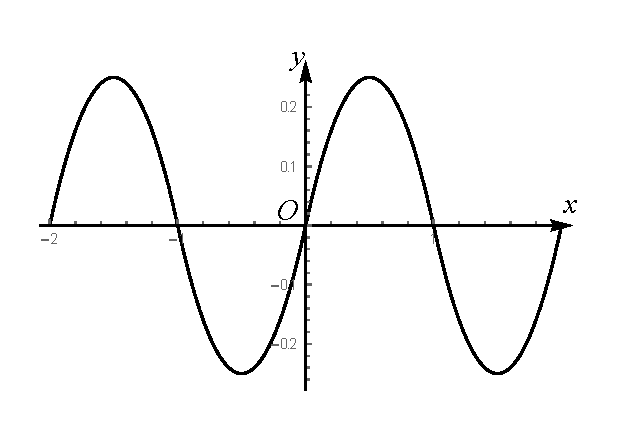
\includegraphics[height=0.3\textheight]{F:/life/2018AutumnTA/Exercises/1/problem3.pdf}
\end{center}
\caption{3.题$f(x)$的图像}
\end{figure}
\item[\bf4.] 设$f(x)$是定义在$(-\infty,+\infty)$上的函数,并且满足$f(2x)=2f(x)$. 试证: 如果$f$在$(-\infty,+\infty)$上有界, 则$f(x)\equiv0$.
\newline
{\bf(反证法. 要证明恒等于0, 只需证明不等于0的$f(x)$不存在, 于是假设存在等于0的点, 推出矛盾.)}
\newline
证明: $\because f(x)$在$(-\infty,+\infty)$上有界, $\therefore\exists M>0,\ \forall x\in(-\infty,+\infty),\ |f(x)|<M$.
\newline
假设$f(x_0)=A\neq0$, 则由$f(2x)=2f(x)$可知$f(2x_0)=2A,f(4x_0)=4A,\dots,f(2^nx_0)=2^nA,\dots,n\in\mathbb Z^+${\bf($|2^nA|$一定会大于$M$, 可解出满足条件的$n$.)}, 取$n>\log_2\frac M{|A|}$, 则$|f(x)|>M$, 矛盾. 故$f(x)\equiv0$.
\item[\bf5.]两个单调增加的函数的复合函数是否一定单调增加? 它们的乘积又如何? 
\newline
{\bf(一定需要证明, 不一定只需给出反例.)}
\newline
解: 两个单调增加的函数的复合函数一定单调增加, 但二者的乘积不一定单调增加. 设这两个函数分别为$f(x),g(x)$, 对于$x_1<x_2$, 有$g(x_1)<g(x_2)$, 则$f(g(x_1))<f(g(x_2))$, 所以$f\circ g(x)$单调增加. 若$f(x_1)=-2,f(x_2)=-1,g(x_1)=1,g(x_2)=3$, 则$f(x_1)g(x_1)=-2>-3=f(x_2)g(x_2)$, 此时$f(x)g(x)$不单调增加.
\item[6.]证明: 函数$\sin|x|,\sin x^2$不是周期函数.
\newline
{\bf(此题较难, 可不讲. 反证法. 提醒同学们不要过分纠结于解题过程的细节, 重要的是把解题思路表达清楚. 比如, “$\therefore$”, “$\Rightarrow$”, “所以”可随意使用.)}
\newline
证明: 若$\sin|x|$是周期函数, 则$\exists T>0,\forall x\in(-\infty,+\infty),\ \sin|x+T|=\sin|x|$, 则当$x=0$时, $\sin T=0$, 则$T=n\pi,n\in\mathbb Z^+$. {\bf(可借助图像帮助理解.)}当$n$为偶数时, $\sin|-\frac\pi2+n\pi|=\sin|\frac{2n-1}2\pi|=\sin\frac{2n-1}2\pi=-1\neq\sin|-\frac\pi2|$, $\therefore\ n$不能为偶数. 当$n$为奇数时, $\sin|\frac\pi2+n\pi|=\sin(\frac\pi2+n\pi)=\sin(\frac\pi2+\pi)=-1\neq\sin|\frac\pi2|$, $\therefore\ n$不能为奇数. 故$T$不存在, 则$\sin|x|$不是周期函数.
\newline
若$\sin x^2$是周期函数, 则$\exists T>0,\forall x\in(-\infty,+\infty),\ \sin(x+T)^2=\sin x^2$, 则当$x=0$时, $\sin T^2=0$, 则$T=\sqrt{n\pi},n\in\mathbb Z^+$. $\sin(-\frac\pi2+\sqrt{n\pi})^2=\sin(\frac{\pi^2}4-\pi\sqrt{n\pi}+n\pi)$, 要使$\sin(-\frac\pi2+\sqrt{n\pi})^2=\sin(-\frac\pi2)^2$, 则必须$-\pi\sqrt{n\pi}+n\pi=2k\pi\text{或}2k\pi+\pi-\frac{\pi^2}2,k\in\mathbb Z$, 解得$n=\frac{1}{2} \left(4 k\pm\sqrt{\pi } \sqrt{8 k+\pi }+\pi \right)\text{或}\frac{1}{2} \left(4 k\pm\sqrt{\pi } \sqrt{8 k+\frac{64 \pi -16 \pi ^2}{16 \pi }}+2\right)$, 不是正整数, 故$T$不存在, 则$\sin x^2$不是周期函数.
\item[\bf7.]设$f(x)$在$[0,+\infty)$上非负. 试证: 如果$f(f(x))$在$[0,+\infty)$上无上界, 则$f(x)$在$[0,+\infty)$上也无上界.
\newline
{\bf(有界性.)}
\newline
证明: $\because f(f(x))$在$[0,+\infty)$上无上界, $\therefore\forall M>0,\exists x_0\in[0,+\infty),f(f(x_0))>M,\ \therefore\forall M>0,$ 当$x=f(x_0)\geq0$时, $f(x)>M$, 故$f(x)$在$[0,+\infty)$上也无上界.
\item[\bf8.] 设$f(x)$是周期等于1的周期函数, 且当$0\leq x<1$时, $f(x)=x^2$. 试写出$f(x)$在$(-\infty,+\infty)$上的表达式, 并作图.
\newline
{\bf(两种表示方式都可以.)}
\newline
解: $f(x)=(x-n)^2,\ n\leq x<1+n,\ n\in\mathbb Z$, 或$f(x)=(x-[x])^2, -\infty<x<+\infty$.
\begin{figure}[H]
\begin{center}
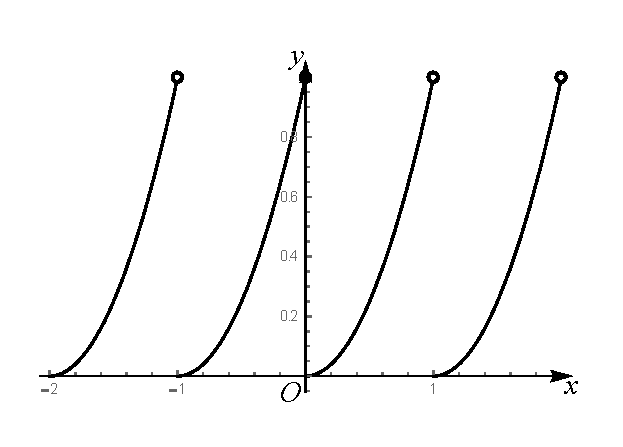
\includegraphics[height=0.3\textheight]{F:/life/2018AutumnTA/Exercises/1/problem8.pdf}
\end{center}
\caption{8.题$f(x)$的图像}
\end{figure}
\item[\bf9.]若已知函数$y=f(x)(-\infty<x<+\infty)$的图形, 试画出$y=f(x-a),\ y=f(ax),\ y=f(x)-a,\ y=af(x)$的图形(自己举一个具体的例子).
\newline
{\bf(口诀: 左加右减, 上加下减; 对于x, 大于1缩小, 小于1放大;  对于y, 大于1放大, 小于1缩小. 也可直观理解.)}
\newline
解:取$f(x)=\sin x,\ a=2.5$.
\begin{figure}[H]
\begin{center}
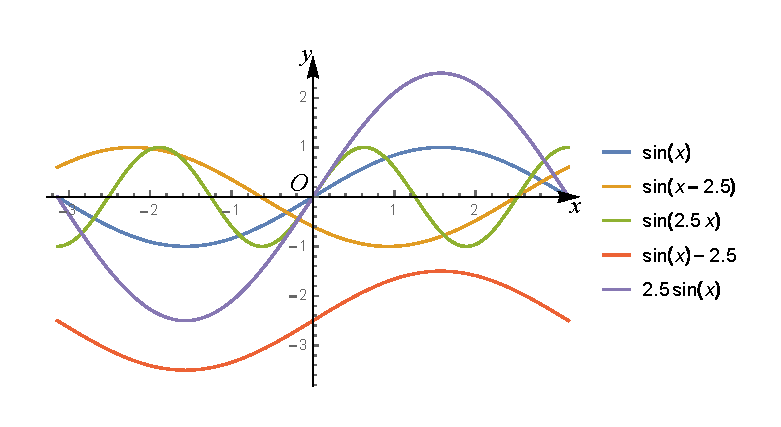
\includegraphics[height=0.3\textheight]{F:/life/2018AutumnTA/Exercises/1/problem9.pdf}
\end{center}
\caption{9.题$f(x)$的图像}
\end{figure}
\item[10.]设$f(x)=\begin{cases}x^2,&x\geq0\\-x^2,&x<0\end{cases}$,试证$f$是$\mathbb R\rightarrow\mathbb R$的一个双射, 并求它的逆映射.
\newline
{\bf(如果$f$既是单射又是满射, 则是双射. 求逆映射就是求反函数. 此题可不讲.)}
\newline
证明: 不妨设$x_1<x_2$, 可分以下三种情况讨论:
\begin{enumerate}
\item[i.]$x_1<x_2\leq0$, 此时$f(x)=-x^2$单调增加, 故$f(x_1)<f(x_2)$;
\item[ii.]$x_1\leq0<x_2$, 此时$f(x_1)\leq0<f(x_2)$;
\item[iii.]$0\leq x_1<x_2$, 此时$f(x)=x^2$单调增加, 故$f(x_1)<f(x_2)$. 
\end{enumerate}
可知$f$是$\mathbb R\rightarrow\mathbb R$的一个单射, 且$f(x)$在$(-\infty,+\infty)$上单调增加. $f(x)$的值域是$(-\infty,+\infty)=\mathbb R$, $\forall y\in\mathbb R,\ \exists x\in\mathbb R,\ \text{使得}y=f(x)$, 故$f$是$\mathbb R\rightarrow\mathbb R$的一个满射. 因此$f$是$\mathbb R\rightarrow\mathbb R$的一个双射. 其逆映射即反函数为
\[
x=\begin{cases}
\sqrt y,&y\geq0\\
\sqrt {-y},&y<0
\end{cases}.
\]
\item[\bf11.]设$f:\ X\rightarrow Y,g:\ Y\rightarrow Z$都是双射.求证$g\circ f:\ X\rightarrow Z$也是双射, 并且$(g\circ f)^{-1}=f^{-1}\circ g^{-1}$.
\newline
{\bf(双射如图所示, 单射和满射的图形也可画出.)}
\begin{figure}[H]
\begin{center}
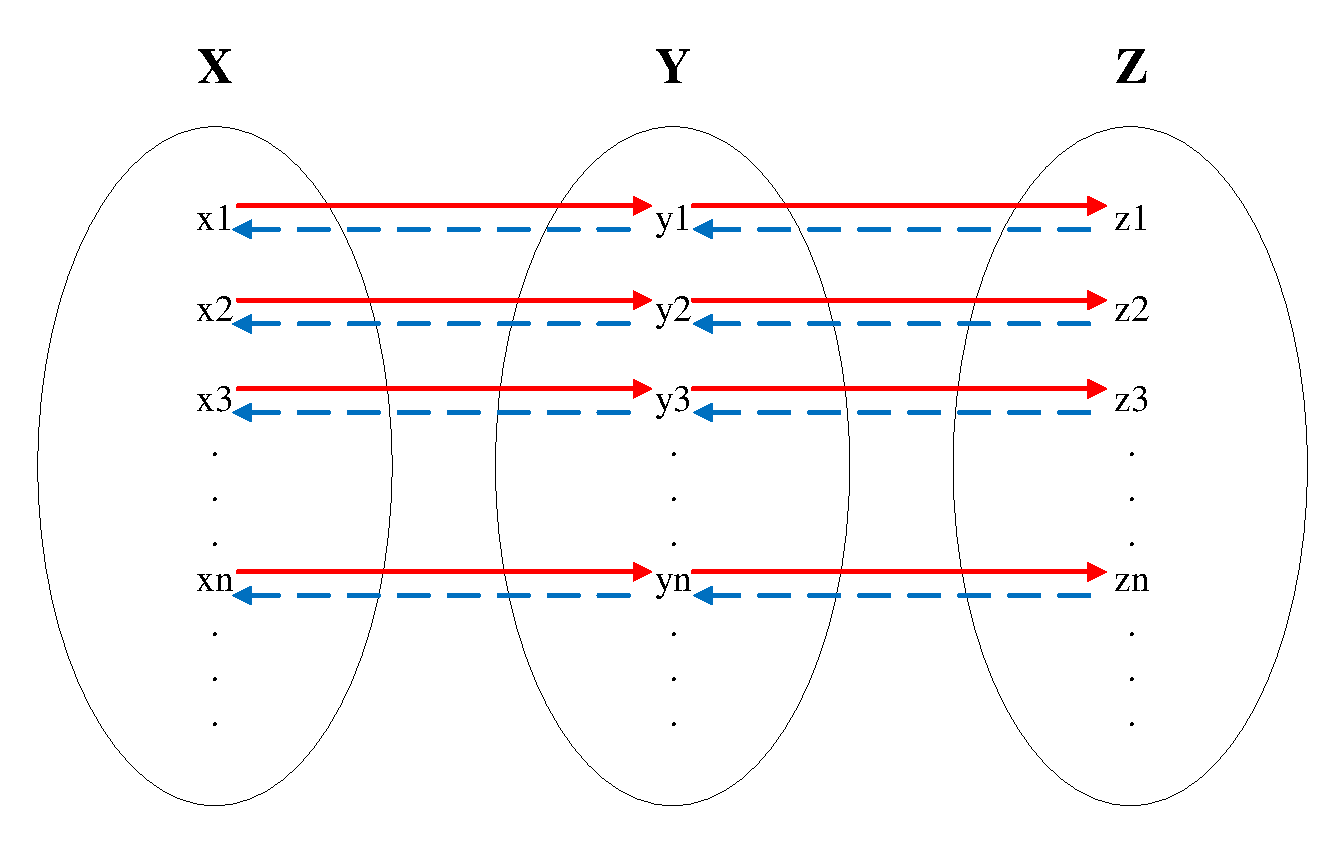
\includegraphics[height=0.3\textheight]{F:/life/2018AutumnTA/Exercises/1/problem11.pdf}
\end{center}
\caption{11.题图示}
\end{figure}


证明: $\because f:\ X\rightarrow Y,g:\ Y\rightarrow Z$都是双射, 
\newline
$\therefore \forall x\in X,\ \exists\text{唯一的} y\in Y,\ \text{满足}y=f(x)$, 对于该$y\in Y,\ \exists\text{唯一的} z\in Z,\ \text{满足}z=g(y)=g(f(x))=g\circ f(x)$; $\forall z\in Z,\ \exists\text{唯一的} y\in Y,\ \text{满足}z=g(y)$, 即$y=g^{-1}(z)$, 对于该$y\in Y,\ \exists\text{唯一的} x\in X,\ \text{满足}y=f(x)$和$z=g(y)=g(f(x))=g\circ f(x)$, 即$x=(g\circ f)^{-1}(z)=f^{-1}(y)=f^{-1}(g^{-1}(z))=f^{-1}\circ g^{-1}(z)$. 
\newline
$\therefore g\circ f:\ X\rightarrow Z$是双射, 且$(g\circ f)^{-1}=f^{-1}\circ g^{-1}$.
\newline
{\bf(结合图示说明.)}
\item[\bf12.]试写出一个从$(0,1)$到$(-\infty,+\infty)$的双射; 写出一个自然数集到整数集的双射.
\newline
解:(1)$y=\cot\pi x,\ 0<x<1$或$y=\tan\pi(x-\frac12),\ 0<x<1${\bf(先伸缩后平移)};
\newline
(2){\bf(构造)}$y=\begin{cases}
k,&x=2k\\
0,&x=0\\
-k,&x=2k-1
\end{cases},x\in\mathbb Z/\mathbb Z^-$.
\end{enumerate}
\subsection{初等函数与非初等函数}
\noindent
\subsubsection{知识结构}
\noindent第一章实数与函数
	\begin{enumerate}
		\item[1.1] 集合与符号
		\item[1.2] 实数和实数集
		\item[1.3] 函数
		\item[1.4] 初等函数
			\begin{itemize}
				\item能用公式表示的函数有两大类:
					\begin{itemize}
						\item初等函数
						\item非初等函数
					\end{itemize}
				\item基本初等函数
					\begin{enumerate}
						\item[1.]常值函数
						\item[2.]幂函数
						\item[3.]指数函数
						\item[4.]对数函数
						\item[5.]三角函数
						\item[6.]反三角函数
					\end{enumerate}
				\item初等函数: 基本初等函数经过有限次四则运算和有限次复合所得到的函数称为初等函数.
					\begin{enumerate}
						\item[7.]双曲函数
					\end{enumerate}
			\end{itemize}
			\item[1.5] 非初等函数: 分段函数、隐函数、用参数式确定的函数, 以及用积分和级数表示的函数等
				\begin{enumerate}
					\item[1.5.1]分段函数
						\begin{itemize}
							\item符号函数
							\item取整函数
						\end{itemize}
					\item[1.5.2]其他非初等函数(隐函数)
						\begin{itemize}
							\item螺线
							\item旋轮线
						\end{itemize}					
				\end{enumerate}
	\end{enumerate}
\subsubsection{双曲正弦}
\begin{enumerate}
	\item双曲正弦$\Rightarrow$反双曲正弦
	\item反双曲正弦$\Rightarrow$双曲正弦, 即习题3
\end{enumerate}
\subsubsection{习题1.4解答}
\begin{enumerate}
\item 求下列函数的定义域:
\newline
$(1)y=\sqrt{x^2-x}\cdot\arcsin x;\hspace{3cm}(2)y=\lg(\lg(\lg x));$
\newline
$(3)y=\arccos e^{2x};\hspace{4.5cm}{\bf(4)}y=\sqrt{\lg(x^2-1)}.$
\newline
{\bf(定义域应写成集合或区间.)}
\newline
解:(1)$y=\sqrt{x^2-x}\cdot\arcsin x,\ \Rightarrow x^2-x\geq0\text{且}-1\leq x\leq1,\ \Rightarrow x(x-1)\geq0\text{且}-1\leq x\leq1,\ \Rightarrow x\geq1\text{或}x\leq0,\text{且}-1\leq x\leq1,\ \Rightarrow x=1\text{或}-1\leq x\leq0,\ \Rightarrow$ 定义域为$[-1,0]\cup\{1\}$.
\newline
(2)$y=\lg(\lg(\lg x)),\ \Rightarrow x>0\text{且}\lg x>0\text{且}\lg(\lg x)>0,\ \Rightarrow x>0\text{且}x>1\text{且}\lg x>1,\ \Rightarrow x>0\text{且}x>1\text{且}x>10,\ \Rightarrow x>10,\ \Rightarrow$ 定义域为$(10,+\infty)$.
\newline
(3)$y=\arccos e^{2x},\ \Rightarrow -1\leq e^{2x}\leq1,\ \Rightarrow 2x\leq0,\ \Rightarrow x\leq0,\ \Rightarrow$ 定义域为$(-\infty,0]$.
\newline
{\bf(4)}$y=\sqrt{\lg(x^2-1)},\ \Rightarrow x^2-1>0\text{且}\lg(x^2-1)>0,\ \Rightarrow x>1\text{或}x<-1,\ \text{且}x^2-1>1,\ \Rightarrow x>1\text{或}x<-1,\ \text{且}x>\sqrt2\text{或}x<-\sqrt2,\ \Rightarrow x>\sqrt2\text{或}x<-\sqrt2,\ \Rightarrow$ 定义域为$(-\infty,\sqrt2)\cup(\sqrt2,+\infty)$.
\item设$f(x)$是定义在$(-\infty,+\infty)$上的奇函数, 在$(0,+\infty)$上的表达式为$f(x)=x-x^2$. 求$f(x)$在$(-\infty,0)$上的表达式.
\newline
解: 当$x<0$时,$f(x)=-f(-x)=-(-x)+(-x)^2=x+x^2.$
\item[\bf3.]验证$y=\ln(\sqrt{x^2+1}+x)$是奇函数, 求这个函数的反函数.
\newline
解: $y(-x)=\ln(\sqrt{x^2+1}-x)=-\ln\frac1{\sqrt{x^2+1}-x}=-\ln\frac{\sqrt{x^2+1}+x}{x^2+1-x^2}=-\ln(\sqrt{x^2+1}+x)=-y(x)$, 故$y=\ln(\sqrt{x^2+1}+x)$是奇函数.
\newline
由$y=\ln(\sqrt{x^2+1}+x)$得$e^y=\sqrt{x^2+1}+x$(*), 由$y(x)=-y(-x)=-\ln(\sqrt{x^2+1}-x)$得$e^{-y}=\sqrt{x^2+1}-x$(**). (*)式和(**)相减可得$x=\frac{e^y-e^{-y}}2$. 反函数为$y=\frac{e^x-e^{-x}}2$.
\item[\bf4.]设$f(x)$是定义在$(-\infty,+\infty)$的函数. 对于任意两个实数$x,y$, 满足$f(x+y)=f(x)+f(y)$. 求证存在常数$a$, 使得对于所有的有理数$x$, 都有$f(x)=ax$.
\newline
{\bf(此题较难, 可不讲.)}
\newline
证明: $\because\forall x,y\in\mathbb R,f(x+y)=f(x)+f(y),\ \therefore f(0)=f(0)+f(0)=0,\ f(x-x)=f(x)+f(-x)=f(0)=0,\ \therefore f(x)=-f(-x),\ \therefore f(x)$是奇函数, 因此只需证明$x>0$的情况. 
\newline
当$x=n,\ n\in\mathbb Z^+$时, $f(2)=f(1)+f(1)=2f(1),\ f(3)=f(2)+f(1)=3f(1),\dots,\ f(n)=nf(1),\dots$, 即$f(x)=f(1)x$;
\newline
当$x=\frac1n,\ n\in\mathbb Z^+$时, $f(1)=f(\frac1n)+f(\frac{n-1}n)=2f(\frac1n)+f(\frac{n-2}n)=\dots=nf(\frac1n),\ \therefore f(\frac1n)=\frac1nf(1)$, 即$f(x)=f(1)x$;
\newline
当$x=\frac mn,\ m,n\in\mathbb Z^+$时, $f(\frac mn)=f(\frac1n)+f(\frac{m-1}n)=mf(\frac1n)=\frac mnf(1)$, 即$f(x)=f(1)x$.
\newline
综上所述, 存在常数$a=f(1)$使得对于所有的有理数x, 都有$f(x)=ax$.
\end{enumerate}
\subsection{补充内容}
维基百科是重要的工具, 上面有各种总结得很好的内容, 可以经常浏览, 拓展知识面. 比如:
\begin{itemize}
	\item 三角函数 \url{https://en.wikipedia.org/wiki/Trigonometric_functions}
	\item 双曲函数 \url{https://en.wikipedia.org/wiki/Hyperbolic_function}
	\item 雅可比椭圆函数 \url{https://en.wikipedia.org/wiki/Jacobi_elliptic_functions}
\end{itemize}
\end{document} 
\documentclass[12pt,UTF8]{ctexart}
\usepackage{ctex,amsmath,amssymb,geometry,fancyhdr,bm,amsfonts
,mathtools,extarrows,graphicx,url,enumerate,color} 
% 加入中文支持
\newcommand\Set[2]{%
\left\{#1\ \middle\vert\ #2 \right\}}
\geometry{a4paper,scale=0.80}
\pagestyle{fancy}
\rhead{习题2.1\&2.2}
\lhead{基础习题课讲义}
\chead{微积分B(1)}
\begin{document}
\setcounter{section}{1}
\section{数列极限}
\noindent
\subsection{知识结构}
\noindent第二章实数与函数
	\begin{enumerate}
		\item[2.1] 数列极限的概念和性质
			\begin{enumerate}
				\item[2.1.1]数列极限的概念
				\item[2.1.2]数列极限的性质
					\begin{itemize}
						\item唯一性
						\item有界性
						\item保号性
					\end{itemize}
				\item[2.1.3]数列的子列
				\item[2.1.4]无穷大量与无界变量
			\end{enumerate}
		\item[2.2] 数列极限存在的条件
			\begin{enumerate}
				\item[2.2.1]夹逼原理
				\item[2.2.2]单调收敛定理
				\item[2.2.3]柯西收敛准则
				\item[2.2.4]数列极限的四则运算
			\end{enumerate}
\end{enumerate}
\subsection{习题2.1解答}
\begin{enumerate}
\item 用数列极限定义证明以下各题:
\newline
$(1)\lim\limits_{n\rightarrow\infty}\frac{5n^3}{1+n^3}=5;$
\newline
$(2)\lim\limits_{n\rightarrow\infty}\frac{\sin n^2}{n}=0.$
\newline
证明:(1){\bf(多项式的标准过程.)}

$\because|\frac{5n^3}{1+n^3}-5|=\frac{5}{1+n^3}$

$\therefore\forall\varepsilon>0,\ \text{取} N>\sqrt[3]{\frac5\varepsilon-1},\ \text{则当}n>N\text{时},\ |\frac{5n^3}{1+n^3}-5|<\varepsilon$

故$\lim\limits_{n\rightarrow\infty}\frac{5n^3}{1+n^3}=5$.
\newline
(2){\bf(常用$\sin x\leq1$.)}

$\because|\frac{\sin n^2}{n}-0|\leq\frac1{n}$

$\therefore\forall\varepsilon>0,\ \text{取}N>\frac1\varepsilon,\ \text{则当}n>N\text{时},\ |\frac{\sin n^2}{n}-0|<\varepsilon$

故$\lim\limits_{n\rightarrow\infty}\frac{\sin n^2}{n}=0$.
\item用极限定义证明以下各题:
\begin{enumerate}[(1)]
	\item若$\lim\limits_{n\rightarrow\infty}a_n=A$,则$\lim\limits_{n\rightarrow\infty}|a_n|=|A|$;
	\item若$\lim\limits_{n\rightarrow\infty}a_n=A>0$,则$\lim\limits_{n\rightarrow\infty}\sqrt{a_n}=\sqrt{A}$;
	\item若$\lim\limits_{n\rightarrow\infty}a_n=A$,则$\lim\limits_{n\rightarrow\infty}a_n^2=A^2$;
	\item若$\lim\limits_{n\rightarrow\infty}a_n=A$,则$\lim\limits_{n\rightarrow\infty}\frac{a_n}n=0$.
\end{enumerate}
{\bf(常用结论的证明.)}
\newline
证明:(1)$||a_n|-|A||\leq|a_n-A|$

$\because\lim\limits_{n\rightarrow\infty}a_n=A$

$\therefore\forall\varepsilon>0,\exists N>0,\ \text{使}n>N$时, $||a_n|-|A||\leq|a_n-A|<\varepsilon$

则$\lim\limits_{n\rightarrow\infty}|a_n|=|A|$.


(2)$\because\lim\limits_{n\rightarrow\infty}a_n=A>0$

$\therefore\exists N_1>0$,使$n>N_1$时,$a_n>0$

$\therefore n>N_1$时,$|\sqrt{a_n}-\sqrt A|=\frac{|a_n-A|}{\sqrt{a_n}+\sqrt A}<\frac{|a_n-A|}{\sqrt A}$

$\because\lim\limits_{n\rightarrow\infty}a_n=A$

$\therefore\forall\varepsilon>0$,$\exists N_2>0$,使$n>N_2$时,$|a_n-A|<\varepsilon$

取$N=\text{max}\{N_1,N_2\}$,当$n>N$时,$|\sqrt{a_n}-\sqrt A|=\frac{|a_n-A|}{\sqrt{a_n}+\sqrt A}<\frac{|a_n-A|}{\sqrt A}<\frac{\varepsilon}{\sqrt A}$

故$\lim\limits_{n\rightarrow\infty}\sqrt{a_n}=\sqrt{A}$.


(3)$|a_n^2-A^2|=|a_n-A||a_n+A|$,

$\because\lim\limits_{n\rightarrow\infty}a_n=A$

$\therefore\exists M>0$,使$|a_n|<M(n>0)$

$\therefore|a_n+A|<|a_n|+|A|<M+|A|$

$\therefore\forall\varepsilon>0,\exists N>0$,当$n>N$时,$|a_n-A|<\varepsilon$

$\therefore|a_n^2-A^2|=|a_n-A||a_n+A|<\varepsilon(M+|A|)$

则$\lim\limits_{n\rightarrow\infty}a_n^2=A^2$.

(4)$\because\lim\limits_{n\rightarrow\infty}a_n=A$

$\therefore\exists M>0$,使$|a_n|<M$

$\forall\varepsilon>0$,取$N>\frac M\varepsilon$,则当$n>N$时,$|\frac{a_n}n-0|<\frac Mn<\varepsilon$.

故$\lim\limits_{n\rightarrow\infty}\frac{a_n}n=0$.
\item设$\lim\limits_{n\rightarrow\infty}a_n=A,\lim\limits_{n\rightarrow\infty}b_n=B$,且$A<B$,则存在正整数$N$,使得当$n>N$时,恒有$a_n<b_n$.
\newline
证明:先证明$\lim\limits_{n\rightarrow\infty}a_n-b_n=A-B$:

$\because\lim\limits_{n\rightarrow\infty}a_n=A,\lim\limits_{n\rightarrow\infty}b_n=B$

$\therefore\forall\varepsilon>0,\exists N_1>0$,使得$n>N_1$时$|a_n-A|<\frac12\varepsilon$,当$n>N_2$时$|b_n-B|<\varepsilon$,当$n>N_2$时$|b_n-B|<\frac12\varepsilon$

取$N=$max$\{N_1,N_2\}$,则当$n>N$时$|a_n-b_n-(A-B)|<|a_n-A|+|b_n-B|<\varepsilon$

$\therefore\lim\limits_{n\rightarrow\infty}a_n-b_n=A-B$.

$\because A<B$

$\therefore A-B<0$

根据数列极限的保号性知存在正整数$N$,使得当$n>N$时,恒有$a_n<b_n$.
\end{enumerate}
\subsection{习题2.2}
\begin{enumerate}
\item用夹逼原理求下列极限
	\begin{enumerate}[(1)]
		\item$\lim\limits_{n\rightarrow\infty}(2+\frac1n)^{\frac1n}$;
		\item$\lim\limits_{n\rightarrow\infty}n^{\frac1n}$;
		\item$\lim\limits_{n\rightarrow\infty}(\frac1{n^2+1}+\frac2{n^2+2}+\cdots+\frac n{n^2+n})$;
		\item$\lim\limits_{n\rightarrow\infty}(\frac1{n^2+1}+\frac1{n^2+2}+\cdots+\frac 1{n^2+n})$.
	\end{enumerate}
证明:(1)$(2+0)^{\frac1n}<(2+\frac1n)^{\frac1n}\leq(2+1)^{\frac1n}$,即$2^{\frac1n}<(2+\frac1n)^{\frac1n}\leq3^{\frac1n}$

$\because\lim\limits_{n\rightarrow\infty}2^{\frac1n}=1,\lim\limits_{n\rightarrow\infty}3^{\frac1n}=1$

$\therefore\lim\limits_{n\rightarrow\infty}(2+\frac1n)^{\frac1n}=1$.

(2)$\because n^{\frac1n}\geq1$

$\therefore a_n=n^{\frac1n}-1\geq0$

$\therefore n=(1+a_n)^n=1+na_n+\frac{n(n+1)}{2!}a_n^2+\cdots>\frac{n(n+1)}{2!}a_n^2(n\geq2)$

$\therefore0<a_n<\sqrt{\frac2{n+1}}(n\geq2)$

$\because\lim\limits_{n\rightarrow\infty}\sqrt{\frac2{n+1}}(n\geq2)=0$

$\therefore\lim\limits_{n\rightarrow\infty}a_n=0$

$\therefore\lim\limits_{n\rightarrow\infty}n^{\frac1n}=1$.

(3)$\frac1{n^2+n}+\frac2{n^2+n}+\cdots+\frac n{n^2+n}<\frac1{n^2+1}+\frac2{n^2+2}+\cdots+\frac n{n^2+n}<\frac1{n^2}+\frac2{n^2}+\cdots+\frac n{n^2}$

即$\frac{\frac{n(n+1)}2}{n^2+n}=\frac12<\frac1{n^2+1}+\frac2{n^2+2}+\cdots+\frac n{n^2+n}<\frac{\frac{n(n+1)}2}{n^2}=\frac{n^2+n}{2n^2}$

$\because\lim\limits_{n\rightarrow\infty}\frac{n^2+n}{2n^2}=\lim\limits_{n\rightarrow\infty}\frac{1+\frac1n}{2}=\frac12$

$\therefore\lim\limits_{n\rightarrow\infty}(\frac1{n^2+1}+\frac2{n^2+2}+\cdots+\frac n{n^2+n})=\frac12$.

(4)$\frac n{\sqrt{n^2+n}}<\frac1{\sqrt{n^2+1}}+\frac1{\sqrt{n^2+2}}+\cdots+\frac 1{\sqrt{n^2+n}}<\frac n{\sqrt{n^2}}=1$

$\because\lim\limits_{n\rightarrow\infty}\frac n{\sqrt{n^2+n}}=\lim\limits_{n\rightarrow\infty}\frac 1{\sqrt{1+\frac1n}}=1$

$\therefore\lim\limits_{n\rightarrow\infty}(\frac1{\sqrt{n^2+1}}+\frac1{\sqrt{n^2+2}}+\cdots+\frac 1{\sqrt{n^2+n}})=1$.
\item用单调收敛定理求下列极限:
	\begin{enumerate}[(1)]
		\item设$x\neq0$,令$a_1=\sin x,a_n=\sin a_{n-1}(n=2,3,\cdots)$,求$\lim\limits_{n\rightarrow\infty}a_n$.
		\item设$a>0,k>0,a_1=\frac12(a+\frac ka),a_n=\frac12(a_{n-1}+\frac k{a_{n-1}})(n=2,3,\cdots)$,求证:$\lim\limits_{n\rightarrow\infty}a_n=\sqrt k$.
		\item设$x_1=a>0,y_1=b>0,x_{n+1}=\sqrt{x_ny_n},y_{n+1}=\frac12(x_n+y_n)(n=1,2,\dots)$. 求证:${x_n}$和${y_n}$收敛于同一个实数.
	\end{enumerate}
(1)解:$a_n-a_{n-1}=\sin a_{n-1}-a_{n-1}$,可分以下两种情况讨论:

(i)当$1\geq a_1=\sin x\geq0$时,$1\geq a_2=\sin a_1\geq0,1\geq a_3=\sin a_2\geq0,\cdots,1\geq a_n=\sin a_{n-1}\geq0,\cdots$

$\therefore a_n-a_{n-1}=\sin a_{n-1}-a_{n-1}\leq0(n=2,3,\cdots)$

$\therefore\{a_n\}$单调非增有下界,故收敛,记$\lim\limits_{n\rightarrow\infty}a_n=A$.

将$a_n=\sin a_{n-1}$两边取极限得$A=\sin A$,即$\lim\limits_{n\rightarrow\infty}a_n=A=0$.

(ii)当$-1\leq a_1=\sin x<0$时,$-1\leq a_2=\sin a_1<0,-1\leq a_3=\sin a_2<0,\cdots,-1\leq a_n=\sin a_{n-1}<0,\cdots$

$\therefore a_n-a_{n-1}=\sin a_{n-1}-a_{n-1}\geq0(n=2,3,\cdots)$

$\therefore\{a_n\}$单调非减有上界,故收敛,记$\lim\limits_{n\rightarrow\infty}a_n=A$.

将$a_n=\sin a_{n-1}$两边取极限得$A=\sin A$,即$\lim\limits_{n\rightarrow\infty}a_n=A=0$.

(2)证明:$a_n-a_{n-1}=\frac12(a_{n-1}+\frac k{a_{n-1}})-a_{n-1}=\frac12(\frac k{a_{n-1}}-a_{n-1})$

$\because a>0$

$\therefore a_1=\frac12(a+\frac ka)>\sqrt k$,$a_2=\frac12(a_1+\frac k{a_1})>\sqrt k,a_3=\frac12(a_2+\frac k{a_2})>\sqrt k,\cdots,a_n=\frac12(a_{n-1}+\frac k{a_{n-1}})>\sqrt k,\cdots$

$\therefore a_n-a_{n-1}=\frac12(\frac k{a_{n-1}}-a_{n-1})<0$

$\therefore\{a_n\}$单调非增有下界,故收敛,记$\lim\limits_{n\rightarrow\infty}a_n=A$.

将$a_n=\frac12(a_{n-1}+\frac k{a_{n-1}})$两边取极限得$A=\frac12(A+\frac kA)$,即$\lim\limits_{n\rightarrow\infty}a_n=A=\sqrt k$.

(3)证明:$y_{n+1}-x_{n+1}=\frac12(x_n+y_n)-\sqrt{x_ny_n}$

$\because a>0,b>0$

$\therefore x_2=\sqrt{ab}>0,y_2=\frac12{a+b}>0,x_3=\sqrt{x_2y_2},y_3=\frac12{x_2+y_2},\cdots,x_n=\sqrt{x_{n-1}y_{n-1}}>0,y_n=\frac12(x_{n-1}+y_{n-1})>0,\cdots$

$\therefore y_{n+1}-x_{n+1}=\frac12(x_n+y_n)-\sqrt{x_ny_n}\geq0(n=1,2,\cdots)$

$\therefore x_n=\sqrt{x_{n-1}y_{n-1}}\geq\sqrt{x_{n-1}x_{n-1}}=x_{n-1},y_n=\frac12(x_{n-1}+y_{n-1})\leq y_{n-1}(n=3,4,\cdots)$

$\therefore x_2=\sqrt{ab}\leq x_3\leq x_4\leq\cdots\leq x_n\leq\cdots,y_2=\frac12(a+b)\geq y_3\geq y_4\geq\cdots\geq y_n\geq\cdots$

且$x_n\leq y_n(n=2,3,\cdots)$

$\therefore\{x_n\},\{y_n\}$均单调有界,故收敛, 记$\lim\limits_{n\rightarrow\infty}x_n=A,\lim\limits_{n\rightarrow\infty}y_n=B$,则$A,B>0$.

将$x_{n+1}=\sqrt{x_ny_n}$和$y_{n+1}=\frac12(x_n+y_n)$两边取极限得$A=\sqrt{AB}$和$B=\frac12(A+B)$,即$A=B$.
\item设数列$\{a_n\}$具有这样的性质:$\forall p\in\mathbb Z^+$,有$\lim\limits_{n\rightarrow\infty}|a_{n+p}-a_n|=0$. 问$\{a_n\}$是不是柯西数列?研究下列数列是否满足上述条件?是否收敛?
\begin{enumerate}[(1)]
	\item$a_n=\sqrt n(n\in\mathbb Z^+)$;
	\item$a_n=\sum_{k=1}^{n}\frac1k$.
\end{enumerate}
解:$\{a_n\}$不一定是柯西数列,根据柯西数列的定义可知柯西数列满足该条件,但满足该条件的数列不一定是柯西数列.如: 

(1)$a_n=\sqrt n(n\in\mathbb Z^+)$,$\forall p\in\mathbb Z^+$,有$\lim\limits_{n\rightarrow\infty}|a_{n+p}-a_n|=\lim\limits_{n\rightarrow\infty}|\sqrt{n+p}-\sqrt n|=\lim\limits_{n\rightarrow\infty}\frac p{\sqrt{n+p}+\sqrt n}=\lim\limits_{n\rightarrow\infty}\frac {\frac p{\sqrt n}}{\sqrt{1+\frac p{n}}+1}=0$,但显然$\{a_n\}$不收敛(因为无界),故不是柯西数列.

(2)$a_n=\sum_{k=1}^{n}\frac1k$,$\forall p\in\mathbb Z^+$,有$\lim\limits_{n\rightarrow\infty}|a_{n+p}-a_n|=\lim\limits_{n\rightarrow\infty}\sum_{k=n+1}^{n+p}\frac1k=\lim\limits_{n\rightarrow\infty}(\frac1{n+1}+\frac1{n+1}+\cdots+\frac1{n+p})=0$,但可证明$\{a_n\}$不收敛,故不是柯西数列.

证明如下:
$\because\ln(1+\frac1k)<\frac1k$

$\therefore a_n=\sum_{k=1}^{n}\frac1k>\sum_{k=1}^{n}\ln(1+\frac1k)=\sum_{k=1}^{n}\ln(1+k)-\ln k=\ln(n+1)$

$\because\ln(n+1)$无上界

$\therefore\{a_n\}$无上界

易知$\{a_n\}$单调增加,故$\{a_n\}$发散.
\item用柯西收敛准则证明下列级数收敛:
\begin{enumerate}[(1)]
	\item$a_n=\sum_{k=1}^n\frac{\sin k}{2^k}(n\in\mathbb Z^+)$;
	\item$a_n=\sum_{k=1}^{n}\frac1{k(k+1)}$
\end{enumerate}
证明:(1)$|a_{n+p}-a_n|=\sum_{k=n+1}^{n+p}\frac{\sin k}{2^k}<\sum_{k=n+1}^{n+p}\frac1{2^k}=\frac1{2^{n+1}}\frac{1-\frac1{2^p}}{1-\frac12}<\frac1{2^n}$

$\therefore\forall\varepsilon>0$,取$N>\log_2\frac1\varepsilon$,当$n>N$时,$\forall p\in\mathbb Z^+,|a_{n+p}-a_n|<\frac1{2^n}<\varepsilon$

$\therefore\{a_n\}$是柯西数列,故收敛.

(2)$|a_{n+p}-a_n|=\sum_{k=n+1}^{n+p}\frac1{k(k+1)}=\frac1{n+1}-\frac1{n+p}<\frac1n$

$\therefore\forall\varepsilon>0$,取$N>\frac1\varepsilon$,当$n>N$时,$\forall p\in\mathbb Z^+,|a_{n+p}-a_n|<\frac1{n}<\varepsilon$

$\therefore\{a_n\}$是柯西数列,故收敛.
\item利用四则运算法则求下列极限:
\begin{enumerate}[(1)]
	\item$\lim\limits_{n\rightarrow\infty}(\frac{1+2+\cdots+n}{n+2}-\frac n2)$;
	\item$\lim\limits_{n\rightarrow\infty}(\sqrt{n^2+n}-n)$;
	\item$\lim\limits_{n\rightarrow\infty}(\sqrt[n]1+\sqrt[n]2+\cdots+\sqrt[n]100)$.
\end{enumerate}
解:(1)$\lim\limits_{n\rightarrow\infty}(\frac{1+2+\cdots+n}{n+2}-\frac n2)=\lim\limits_{n\rightarrow\infty}[\frac{\frac{n(n+1)}2}{n+2}-\frac n2]=\lim\limits_{n\rightarrow\infty}[\frac{n(n+1)}{2(n+2)}-\frac n2]=\lim\limits_{n\rightarrow\infty}[\frac{-n}{2(n+2)}]=\lim\limits_{n\rightarrow\infty}[\frac{-1}{2(1+\frac2n)}]=-\frac12$.

(2)$\lim\limits_{n\rightarrow\infty}(\sqrt{n^2+n}-n)=\lim\limits_{n\rightarrow\infty}\frac{n^2+n-n^2}{\sqrt{n^2+n}+n}=\lim\limits_{n\rightarrow\infty}\frac{1}{\sqrt{1+\frac1n}+1}=\frac12$.

(3)$\lim\limits_{n\rightarrow\infty}(\sqrt[n]1+\sqrt[n]2+\cdots+\sqrt[n]{100})=\lim\limits_{n\rightarrow\infty}\sqrt[n]1+\lim\limits_{n\rightarrow\infty}\sqrt[n]2+\cdots+\lim\limits_{n\rightarrow\infty}\sqrt[n]{100}=1+1+\cdots+1=100$.

\item设$a_n\neq0(n\in\mathbb Z^+),\lim\limits_{n\rightarrow\infty}|\frac{a_{n+1}}{a_n}|=q<1$,求证:$\lim\limits_{n\rightarrow\infty}{a_n}=0$.

解:$\because \lim\limits_{n\rightarrow\infty}|\frac{a_{n+1}}{a_n}|=q$

$\therefore \forall \varepsilon>0,\ \exists N>0,\ \text{使得}n>N\text{时},\ ||\frac{a_{n+1}}{a_n}|-q|<\varepsilon$

$\therefore  |\frac{a_{n+1}}{a_n}|<q+\varepsilon$

$\text{可知当}\varepsilon\text{足够小时}, |\frac{a_{n+1}}{a_n}|<q+\varepsilon<1(n>N), \text{即在}n>N\text{时, 数列}\{|a_n|\}\text{单调减少}$

$\because a_n\neq0$

$\therefore \lim\limits_{n\rightarrow\infty}|a_n|\text{存在}$

$\therefore\lim\limits_{n\rightarrow\infty}|a_{n+1}|=\lim\limits_{n\rightarrow\infty}|a_{n}|$

$\therefore \lim\limits_{n\rightarrow\infty}|a_{n+1}|=q\lim\limits_{n\rightarrow\infty}|a_{n}|=\lim\limits_{n\rightarrow\infty}|a_n|,\ \text{即}\lim\limits_{n\rightarrow\infty}|a_n|(1-q)=0$

$\because q<1$

$\therefore 1-q\neq0$

$\therefore\lim\limits_{n\rightarrow\infty}|a_n|=0$

$\therefore \forall \varepsilon>0,\ \exists N>0,\ \text{使得}n>N\text{时},\ |a_n|-0<\varepsilon,\ \text{即}|a_n-0|<\varepsilon$

$ \therefore\lim\limits_{n\rightarrow\infty}a_n=0$.

\item利用上题结论证明下列结论:
\begin{enumerate}[(1)]
	\item$\lim\limits_{n\rightarrow\infty}\frac{a^n}{n!}=0(a>0)$;
	\item$\lim\limits_{n\rightarrow\infty}\frac{n^2}{a^n}=0(a>1)$;
	\item$\lim\limits_{n\rightarrow\infty}\frac{a^n}{(n!)^2}=0(a>0)$.
\end{enumerate}
证明:(1)$a_n=\frac{a^n}{n!},\lim\limits_{n\rightarrow\infty}|\frac{a_{n+1}}{a_n}|=\lim\limits_{n\rightarrow\infty}\frac a{n+1}=0<1(a>0)$,故$\lim\limits_{n\rightarrow\infty}\frac{a^n}{n!}=0$.

(2)$a_n=\frac{n^2}{a^n},\lim\limits_{n\rightarrow\infty}|\frac{a_{n+1}}{a_n}|=\lim\limits_{n\rightarrow\infty}\frac1a\frac{(n+1)^2}{n^2}=\frac1a<1(a>1)$,故$\lim\limits_{n\rightarrow\infty}\frac{n^2}{a^n}=0$.

(3)$a_n=\frac{a^n}{(n!)^2},\lim\limits_{n\rightarrow\infty}|\frac{a_{n+1}}{a_n}|=\lim\limits_{n\rightarrow\infty}\frac a{(n+1)^2}=0<1(a>0)$,故$\lim\limits_{n\rightarrow\infty}\frac{a^n}{(n!)^2}=0$.
\item求极限:
\begin{enumerate}[(1)]
	\item$\lim\limits_{n\rightarrow\infty}\sin^2(\pi\sqrt{n^2+1})$;
	\item$\lim\limits_{n\rightarrow\infty}\sin^2(\pi\sqrt{n^2+n})$.
\end{enumerate}
解:(1)$\lim\limits_{n\rightarrow\infty}\sin^2(\pi\sqrt{n^2+1})=\lim\limits_{n\rightarrow\infty}\sin^2(\pi\sqrt{n^2+1}-\pi n)=\lim\limits_{n\rightarrow\infty}\sin^2\frac{\pi}{\sqrt{n^2+1}+n}=\sin^20=0$.

(2)$\lim\limits_{n\rightarrow\infty}\sin^2(\pi\sqrt{n^2+n})=\lim\limits_{n\rightarrow\infty}\sin^2(\pi\sqrt{n^2+n}-\pi n)=\lim\limits_{n\rightarrow\infty}\sin^2\frac{\pi n}{\sqrt{n^2+n}+n}=\lim\limits_{n\rightarrow\infty}\sin^2\frac{\pi}{\sqrt{1+\frac1n}+1}=\sin^2\frac\pi2=1$.


{\bf(这里用到了结论:若$\lim\limits_{n\rightarrow\infty}a_n=A$,则$\lim\limits_{n\rightarrow\infty}\sin^2a_n=\sin^2A$.)}
\end{enumerate}
\end{document} 
\documentclass[12pt,UTF8]{ctexart}
\usepackage{ctex,amsmath,amssymb,geometry,fancyhdr,bm,amsfonts
,mathtools,extarrows,graphicx,url,enumerate,color} 
% 加入中文支持
\newcommand\Set[2]{%
\left\{#1\ \middle\vert\ #2 \right\}}
\geometry{a4paper,scale=0.80}
\pagestyle{fancy}
\rhead{习题2.3\&2.4\&2.5\&第2章补充题}
\lhead{基础习题课讲义}
\chead{微积分B(1)}
\begin{document}
\setcounter{section}{2}
\section{函数极限与无穷小量}
\noindent
\subsection{知识结构}
\noindent第二章极限论
	\begin{enumerate}
		\item[2.1] 数列极限的概念和性质
			\begin{enumerate}
				\item[2.1.1]数列极限的概念
				\item[2.1.2]数列极限的性质
					\begin{itemize}
						\item唯一性
						\item有界性
						\item保号性
					\end{itemize}
				\item[2.1.3]数列的子列
				\item[2.1.4]无穷大量与无界变量
			\end{enumerate}
		\item[2.2] 数列极限存在的条件
			\begin{enumerate}
				\item[2.2.1]夹逼原理
				\item[2.2.2]单调收敛定理
				\item[2.2.3]柯西收敛准则
				\item[2.2.4]数列极限的四则运算
			\end{enumerate}
		\item[2.3] 函数极限的概念和性质
			\begin{enumerate}
				\item[2.3.1]函数在一点的极限
				\item[2.3.2]单侧极限
				\item[2.3.3]函数在无穷远处的极限
				\item[2.3.4]函数极限的性质
					\begin{itemize}
						\item唯一性
						\item有界性
						\item保号性
						\item函数极限与数列极限的关系
					\end{itemize}
			\end{enumerate}
		\item[2.4] 函数极限的运算法则
			\begin{enumerate}
				\item[2.4.1]夹逼原理
				\item[2.4.2]单调函数的极限
				\item[2.4.3]函数极限的四则运算
				\item[2.4.4]极限的复合运算
			\end{enumerate}
		\item[2.5] 无穷小量与阶的比较
			\begin{enumerate}
				\item[2.5.1]无穷小量与无穷大量
				\item[2.5.2]阶的比较
			\end{enumerate}
\end{enumerate}
\subsection{习题2.3解答}
\begin{enumerate}
\item 用定义证明以下各式:
\newline
$(1)\lim\limits_{x\rightarrow x_0}\sin x=\sin x_0$;
\newline
$(2)\lim\limits_{h\rightarrow0}\frac{(x+h)^2-x^2}h=2x$;
\newline
$(3)\lim\limits_{x\rightarrow2}\sqrt{x^2+5}=3$;
\newline
$(4)\lim\limits_{x\rightarrow3}\frac{x-3}{x^2-9}=\frac16$;
\newline
$(5)\lim\limits_{x\rightarrow1^+}\frac{x-1}{x^2-1}=0$;
\newline
$(6)\lim\limits_{x\rightarrow-\infty}(x+\sqrt{x^2-a})=0$.
\newline
解:(1)$|\sin x-\sin x_0|=2|\cos\frac{x+x_0}2||\sin\frac{x-x_0}2|\leq2|\sin\frac{x-x_0}2|\leq|x-x_0|$

$\forall\varepsilon>0$,取$\delta=\varepsilon>0$,使$0<|x-x_0|<\delta$时,$|\sin x-\sin x_0|\leq|x-x_0|<\varepsilon$

$\therefore\lim\limits_{x\rightarrow x_0}\sin x=\sin x_0$.

(2)$|\frac{(x+h)^2-x^2}h-2x|=|\frac{(x+h+x)(x+h-x)}h-2x|=|h|$

$\forall\varepsilon>0$,取$\delta=\varepsilon>0$,使$0<|x-x_0|<\delta$时,$|\frac{(x+h)^2-x^2}h-2x|=|h|<\varepsilon$

$\therefore\lim\limits_{h\rightarrow0}\frac{(x+h)^2-x^2}h=2x$

(3)$|\sqrt{x^2+5}-3|=\frac{|x-2||x+2|}{\sqrt{x^2+5}+3}<|x-2||x+2|$

不妨设$|x-2|<\frac12$,则$\forall\varepsilon>0$,取$\delta={\rm min}\{\frac12,\frac29\varepsilon\}$,则当$0<|x-2|<\delta$时,$|\sqrt{x^2+5}-3|<|x-2||x+2|<\frac92|x-2|<\varepsilon$

$\therefore\lim\limits_{x\rightarrow2}\sqrt{x^2+5}=3$.

(4)$|\frac{x-3}{x^2-9}-\frac16|=\frac{|x^2-6x+9|}{6|x^2-9|}=\frac{|x-9|}{6|x+9|}$

不妨设$|x-3|<\frac12$,即$\frac52<x<\frac72,\frac{11}2<x<\frac{13}2$,取$\delta={\rm min}\{\frac12,33\varepsilon\}$,则当$0<|x-3|<\delta$时,$|\frac{x-3}{x^2-9}-\frac16|=\frac{|x-9|}{6|x+9|}<\frac{|x-9|}{33}<\varepsilon$

$\therefore\lim\limits_{x\rightarrow3}\frac{x-3}{x^2-9}=\frac16$.

(5)当$x>1$时,$|\frac{x-1}{\sqrt{x^2-1}}|=|\frac{\sqrt{x-1}}{\sqrt{x+1}}|<\frac{\sqrt{x-1}}2$

$\forall\varepsilon>0$,取$\delta=2\varepsilon^2$,则当$0<x-1<\delta$时,$|\frac{x-1}{\sqrt{x^2-1}}|<\frac{\sqrt{x-1}}2<\varepsilon$

$\therefore\lim\limits_{x\rightarrow1^+}\frac{x-1}{x^2-1}=0$.

(6)当$x<0$时,$|x+\sqrt{x^2-a}|=\frac{|a|}{-x+\sqrt{x^2-a}}<\frac{|a|}{-x}$

$\forall\varepsilon>0$,取$N>\frac{|a|}\varepsilon>0$,则当$-x>N$时,$|x+\sqrt{x^2-a}|<\frac{|a|}{-x}<\varepsilon$

$\therefore\lim\limits_{x\rightarrow-\infty}(x+\sqrt{x^2-a})=0$.

\item讨论以下函数在点$x=0$的极限是否存在:
\newline
$(1)f(x)=\frac{|x|}x$;
\newline
$f(x)=\begin{cases}\sin\frac1x,&x>0\\
x\sin\frac1x,&x<0
\end{cases}$;
\newline
$f(x)=\frac{[x]}x$;
\newline
$f(x)=\begin{cases}
2x,&x>0\\
a\cos x+b\sin x,&x<0
\end{cases}$.

解:(1)不存在. 当$x<0$时,$f(x)=-1,\lim\limits_{x\rightarrow0^-}=-1$,当$x>0$时,$f(x)=1,\lim\limits_{x\rightarrow0^+}=1\neq\lim\limits_{x\rightarrow1^-}$,故$f(x)$在点$x=0$的极限不存在.

(2)不存在. 当$x>0$时,$\lim\limits_{x\rightarrow0^+}\sin\frac1x$不存在,故$f(x)$在点$x=0$的极限不存在.

(3)不存在. 当$x>0$时,$f(x)=0,\lim\limits_{x\rightarrow0^+}f(x)=0$,当$x<0$时,$f(x)=-\frac1x,\lim\limits_{x\rightarrow0^-}f(x)$不存在,故$f(x)$在点$x=0$的极限不存在.

(4)当$a=0$时存在,当$a\neq0$时不存在. $\lim\limits_{x\rightarrow0+}f(x)=0,\lim\limits_{x\rightarrow0-}f(x)=a$,当$a=0$时,$\lim\limits_{x\rightarrow0+}f(x)=\lim\limits_{x\rightarrow0-}f(x)$,故$f(x)$在点$x=0$的极限存在,当$a\neq0$时,$\lim\limits_{x\rightarrow0+}f(x)\neq\lim\limits_{x\rightarrow0-}f(x)$,故$f(x)$在点$x=0$的极限不存在.

\item设$\lim\limits_{x\rightarrow x_0}f(x)=A>0$,证明$\lim\limits_{x\rightarrow x_0}\sqrt{f(x)}=\sqrt A$.

证明:$\because\lim\limits_{x\rightarrow x_0}f(x)=A>0$

$\therefore\forall\varepsilon>0,\exists\delta_1>0$,当$0<|x-x_0|<\delta_1$时,$|f(x)-A|<\varepsilon$,$\exists\delta_2>0$,当$0<|x-x_0|<\delta_2$时,$f(x)>0$

取$\delta=\text{min}\{\delta_1,\delta_2\}$,则当$0<|x-x_0|<\delta$时,$|\sqrt{f(x)}-\sqrt A|=\frac{|f(x)-A|}{\sqrt{f(x)}+\sqrt A}<\frac{|f(x)-A|}{\sqrt A}<\frac\varepsilon{\sqrt A}$

$\therefore\lim\limits_{x\rightarrow x_0}\sqrt{f(x)}=\sqrt A$.

\item设$f(x)$在$[0,+\infty)$上为周期函数,若$\lim\limits_{x\rightarrow+\infty}f(x)=0$,证明$f(x)\equiv0$.

证明:假设存在$x_0\in[0,+\infty)$,使得$f(x_0)\neq0$

$\because f(x)$在$[0,+\infty)$上是周期函数,设$T$是$f(x)$的最小正周期,则$f(x_0+nT)=f(x_0),n\in\mathbb Z^+$

$\because\lim\limits_{x\rightarrow+\infty}\sqrt{f(x)}=0$

$\therefore\forall\varepsilon>0,\exists N>0$,使$x>N$时,$|f(x)-A|<\varepsilon$

但对于$\varepsilon=\frac12|f(x_0)|,\forall N>0,\exists x=x_0+nT\in\mathbb Z^+$,使得$x>N$时,$|f(x)-0|=|f(x_0+nT)-0|=|f(x_0)-0|>\varepsilon$,矛盾.

故$f(x)\equiv0$.
\end{enumerate}
\subsection{习题2.4解答}
\begin{enumerate}
\item求下列极限:
\newline
$(1)\lim\limits_{x\rightarrow+\infty}\frac{1-x-4x^3}{1+x^2+2x^3}$;
\newline
$(2)\lim\limits_{x\rightarrow0}\frac{\sqrt{1+x}-\sqrt{1-x}}x$;
\newline
$(3)\lim\limits_{x\rightarrow1}\frac{x+x^2+\cdots+x^n-n}{x-1}$;
\newline
$(4)\lim\limits_{x\rightarrow1}\frac{x^m-1}{x^n-1},m,n\in\mathbb Z^+$;
\newline
$(5)\lim\limits_{x\rightarrow+\infty}(\sqrt{x+1}-\sqrt{x-1})$;
\newline
$(6)\lim\limits_{x\rightarrow0}\frac{\sqrt{x^2+p^2}-p}{\sqrt{x^2+q^2}-q}(p>0,q>0)$.

解:(1)$\lim\limits_{x\rightarrow+\infty}\frac{1-x-4x^3}{1+x^2+2x^3}=\lim\limits_{x\rightarrow+\infty}\frac{\frac1{x^3}-\frac1{x^2}-4}{\frac1{x^3}+\frac1x+2}=-2$.

(2)$\lim\limits_{x\rightarrow0}\frac{\sqrt{1+x}-\sqrt{1-x}}x=\lim\limits_{x\rightarrow0}\frac{2x}{x(\sqrt{1+x}+\sqrt{1-x})}=\lim\limits_{x\rightarrow0}\frac2{\sqrt{1+x}+\sqrt{1-x}}=1$.

(3)$\lim\limits_{x\rightarrow1}\frac{x+x^2+\cdots+x^n-n}{x-1}=\lim\limits_{x\rightarrow1}\frac{(x-1)+(x^2-1)+\cdots+(x^n-1)}{x-1}=\lim\limits_{x\rightarrow1}[1+(x+1)+\cdots+(x^{n-1}+x^{n-2}+\cdots+x+1)]=1+2+\cdots+n=\frac{n(n+1)}2$.

(4)$\lim\limits_{x\rightarrow1}\frac{x^m-1}{x^n-1}=\lim\limits_{x\rightarrow1}\frac{(x-1)(x^{m-1}+x^{m-2}+\cdots+x+1)}{(x-1)(x^{n-1}+x^{n-2}+\cdots+x+1)}=\lim\limits_{x\rightarrow1}\frac{x^{m-1}+x^{m-2}+\cdots+x+1}{x^{n-1}+x^{n-2}+\cdots+x+1}=\frac mn$.

(5)$\lim\limits_{x\rightarrow+\infty}(\sqrt{x+1}-\sqrt{x-1})=\lim\limits_{x\rightarrow+\infty}\frac{2}{\sqrt{x+1}+\sqrt{x-1}}=0$.

(6)$\lim\limits_{x\rightarrow0}\frac{\sqrt{x^2+p^2}-p}{\sqrt{x^2+q^2}-q}=\lim\limits_{x\rightarrow0}\frac{x^2+p^2-p^2}{x^2+q^2-q^2}\frac{\sqrt{x^2+q^2}+q}{\sqrt{x^2+p^2}+p}=\lim\limits_{x\rightarrow0}\frac{\sqrt{x^2+q^2}+q}{\sqrt{x^2+p^2}+p}=\frac qp$.

\item求下列极限:
\newline
(1)$\lim\limits_{x\rightarrow0}\frac{\sin2x}{x}$;
\newline
(2)$\lim\limits_{x\rightarrow0}\frac{\sin x^3}{(\sin x)^3}$;
\newline
(3)$\lim\limits_{x\rightarrow0}\frac{\sin ax}{\sin bx}(b\neq0)$;
\newline
(4)$\lim\limits_{x\rightarrow\frac\pi2}\frac{\cos x}{x-\frac\pi2}$;
\newline
(5)$\lim\limits_{x\rightarrow0}\frac{\tan x}x$;
\newline
(6)$\lim\limits_{x\rightarrow0}\frac{\arctan x}x$;
\newline
(7)$\lim\limits_{x\rightarrow0}\frac{\tan x-\sin x}{x^3}$;
\newline
(8)$\lim\limits_{x\rightarrow9}\frac{\sin^2x-\sin^29}{x-9}$;
\newline
(9)$\lim\limits_{x\rightarrow0}\frac{\sin4x}{\sqrt{x+1}-1}$;
\newline
(10)$\lim\limits_{x\rightarrow0}\frac{\sin(\tan x)}{\sin x}$;
\newline
(11)$\lim\limits_{x\rightarrow0}(1+kx)^{\frac1x}$;
\newline
(12)$\lim\limits_{x\rightarrow\infty}(\frac{x+n}{x-n})^x$;
\newline
(13)$\lim\limits_{x\rightarrow0}\frac(1+\tan x)^{\cot x}$;
\newline
(14)$\lim\limits_{x\rightarrow\infty}(1-\frac kx)^{mx}$.

解:(1)$\lim\limits_{x\rightarrow0}\frac{\sin2x}{x}=\lim\limits_{x\rightarrow0}\frac{\sin2x}{2x}2=2$.

(2)$\lim\limits_{x\rightarrow0}\frac{\sin x^3}{(\sin x)^3}=\lim\limits_{x\rightarrow0}\frac{\sin x^3}{x^3}\frac{x^3}{(\sin x)^3}=1$.

(3)$\lim\limits_{x\rightarrow0}\frac{\sin ax}{\sin bx}=\lim\limits_{x\rightarrow0}\frac{\sin ax}{ax}\frac{bx}{\sin bx}\frac ab=\frac ab$.

(4)$\lim\limits_{x\rightarrow\frac\pi2}\frac{\cos x}{x-\frac\pi2}\xlongequal{t=x-\frac\pi2}\lim\limits_{t\rightarrow0}\frac{\cos(t+\frac\pi2)}t\lim\limits_{t\rightarrow0}\frac{-\sin t}t=-1$.

(5)$\lim\limits_{x\rightarrow0}\frac{\tan x}x=\lim\limits_{x\rightarrow0}\frac{\sin x}x\frac1{\cos x}=1$.

(6)$\lim\limits_{x\rightarrow0}\frac{\arctan x}x\xlongequal{t=\arctan x}\lim\limits_{t\rightarrow0}\frac{t}\tan t=1$.

(7)$\lim\limits_{x\rightarrow0}\frac{\tan x-\sin x}{x^3}=\lim\limits_{x\rightarrow0}\frac{\sin x}{x}\frac{1-\cos x}{x^2}\frac1{\cos x}=\lim\limits_{x\rightarrow0}\frac{\tan x-\sin x}{x^3}=\lim\limits_{x\rightarrow0}\frac{\sin x}{x}\frac{1-\cos x}{x^2}\frac1{\cos x}=\lim\limits_{x\rightarrow0}\frac{\sin x}{x}\frac{\sin^2{\frac x2}}{(\frac x2)^2}\frac1{\cos x}\frac12=\frac12$.

(8)$\lim\limits_{x\rightarrow9}\frac{\sin^2x-\sin^29}{x-9}=\lim\limits_{x\rightarrow9}\frac{(\sin x-\sin9)(\sin x+\sin9)}{x-9}=\lim\limits_{x\rightarrow9}\frac{(2\cos\frac{x+9}2\sin\frac{x-9}2)(\sin x+\sin9)}{x-9}=\lim\limits_{x\rightarrow9}(\cos\frac{x+9}2)(\sin x+\sin9)\frac{\sin\frac{x-9}2}{\frac{x-9}2}=2\sin9\cos9=\sin18$.

(9)$\lim\limits_{x\rightarrow0}\frac{\sin4x}{\sqrt{x+1}-1}=\lim\limits_{x\rightarrow0}\frac{\sin4x}{4x}4(\sqrt{x+1}+1)=8$.

(10)$\lim\limits_{x\rightarrow0}\frac{\sin(\tan x)}{\sin x}=\lim\limits_{x\rightarrow0}\frac{\sin(\tan x)}{\tan x}\frac{1}{\cos x}=1$.

(11)$\lim\limits_{x\rightarrow0}(1+kx)^{\frac1x}=\lim\limits_{x\rightarrow0}[(1+kx)^{\frac1{kx}}]^k=e^k$.

(12)$\lim\limits_{x\rightarrow\infty}(\frac{x+n}{x-n})^x=\lim\limits_{x\rightarrow\infty}[(1+\frac{2n}{x-n})^{\frac{x-n}{2n}}]^{2n}(1+\frac{2n}{x-n})^n=e^{2n}$.

(13)$\lim\limits_{x\rightarrow0}(1+\tan x)^{\cot x}=\lim\limits_{x\rightarrow0}(1+\tan x)^{\frac1{\tan x}}=e$.

(14)$\lim\limits_{x\rightarrow\infty}(1-\frac kx)^{mx}=\lim\limits_{x\rightarrow\infty}[(1-\frac kx)^{\frac xk}]^{mk}=e^{-mk}$.

\item确定$a,b$,使下列各式成立:
\newline
(1)$\lim\limits_{x\rightarrow+\infty}(\frac{1+x^2}{1+x}-ax-b)=0$;
\newline
(2)$\lim\limits_{x\rightarrow-\infty}(\sqrt{x^2-x+1}-ax-b)=0$.

解:(1)$\because\lim\limits_{x\rightarrow+\infty}(\frac{1+x^2}{1+x}-ax-b)=\lim\limits_{x\rightarrow+\infty}\frac{1+x^2-ax^2-(a+b)x-b}{1+x}=\lim\limits_{x\rightarrow+\infty}\frac{(1-a)x^2-(a+b)x+1-b}{1+x}\\=\lim\limits_{x\rightarrow+\infty}\frac{(1-a)x-(a+b)+\frac{1-b}x}{\frac1x+1}=0$

$\therefore 1-a=0$且$a+b=0$

$\therefore a=1,b=-1$.

(2)$\because\lim\limits_{x\rightarrow-\infty}(\sqrt{x^2-x+1}-ax-b)=\lim\limits_{x\rightarrow-\infty}\frac{x^2-x+1-(ax+b)^2}{\sqrt{x^2-x+1}+ax+b}=\lim\limits_{x\rightarrow-\infty}\frac{(1-a^2)x^2-(1+2ab)x+1-b^2}{\sqrt{x^2-x+1}+ax+b}\\
=\lim\limits_{x\rightarrow-\infty}\frac{-(1-a^2)x+(1+2ab)-\frac{1-b^2}{x}}{\sqrt{1-\frac1x+\frac1{x^2}}-a-\frac bx}=0$

$\because$如果$1-a^2\neq0$,则极限$\lim\limits_{x\rightarrow-\infty}\frac{-(1-a^2)x+(1+2ab)-\frac{1-b^2}{x}}{\sqrt{1-\frac1x+\frac1{x^2}}-a-\frac bx}$不存在

$\therefore 1-a^2=0$

$\therefore \lim\limits_{x\rightarrow-\infty}\frac{-(1-a^2)x+(1+2ab)-\frac{1-b^2}{x}}{\sqrt{1-\frac1x+\frac1{x^2}}-a-\frac bx}=\frac{1+2ab}{1-a}=0$

$\therefore 1+2ab=0$且$1-a\neq0$

$\therefore a=-1,b=\frac12$.

\item求极限:
\newline
(1)$\lim\limits_{x\rightarrow0}(2\sin x+\cos x)^{\frac1x}$;
\newline
(2)$\lim\limits_{x\rightarrow0}\frac{\sin2x}{\sqrt{x+2}-\sqrt2}$.

解:(1)$\lim\limits_{x\rightarrow0}(2\sin x+\cos x)^{\frac1x}=\lim\limits_{x\rightarrow0}(\cos x)^{\frac1x}(1+2\tan x)^{\frac1x}=\lim\limits_{x\rightarrow0}(1-2\sin^2\frac{x}2)^{\frac1x}[(1+2\tan x)^{\frac1{2\tan x}}]^{\frac{2\tan x}x}=\lim\limits_{x\rightarrow0}(1-\sqrt2\sin\frac{x}2)^{\frac1x}(1+\sqrt2\sin\frac{x}2)^{\frac1x}[(1+2\tan x)^{\frac1{2\tan x}}]^{\frac{2\tan x}x}=\lim\limits_{x\rightarrow0}[(1-\sqrt2\sin\frac{x}2)^{\frac1{\sqrt2\sin\frac{x}2}}]^{\frac{\sqrt2\sin\frac{x}2}x}[(1+\sqrt2\sin\frac{x}2)^{\frac1{\sqrt2\sin\frac{x}2}}]^{\frac{\sqrt2\sin\frac{x}2}x}[(1+2\tan x)^{\frac1{2\tan x}}]^{\frac{2\tan x}x}=e^{-\frac{\sqrt2}2}e^{\frac{\sqrt2}2}e^2=e^2$.

(2)$\lim\limits_{x\rightarrow0}\frac{\sin2x}{\sqrt{x+2}-\sqrt2}=\lim\limits_{x\rightarrow0}\frac{\sin2x(\sqrt{x+2}+\sqrt2)}{x}=4\sqrt2$.

\item分析下面两个函数的极限,说明定理2.4.4中的条件“当$t\neq t_0$时,$g(t)\neq x_0$”是不可缺少的.
\newline
(1)$f(x)=\frac{\sin x}x,g(t)=t\sin\frac1t,x_0=0,t_0=0$;
\newline
(2)$f(x)=\begin{cases}
\frac{\sin x}x,&x\neq0\\
0,&x=0
\end{cases},g(t)=t\sin\frac1t,x_0=0,t_0=0$.

解:(1)$\lim\limits_{x\rightarrow0}f(x)=1,\lim\limits_{t\rightarrow0}g(t)=0$,但$\lim\limits_{t\rightarrow0}f(g(t))=\lim\limits_{t\rightarrow0}\frac{\sin(t\sin\frac1t)}{t\sin\frac1t}$不存在. 因为$\forall\varepsilon>0,\forall\delta>0$,当$0<|t-0|<\delta$时,存在无穷多个点$t=\frac1{n\pi},n>\frac1{\delta\pi},n\in\mathbb Z^+$,使得$g(t)=t\sin\frac1t=0$,从而$f(g(t))=\frac{\sin g(t)}{g(t)}$在这些点处无定义,因而极限不存在. 故虽满足$\lim\limits_{t\rightarrow t_0}g(t)=x_0,\lim\limits_{x\rightarrow x_0}f(x)=A$,但因不满足“当$t\neq t_0$时,$g(t)\neq x_0$”,可导致复合函数的极限$\lim\limits_{t\rightarrow t_0}f(g(t))$不存在.

(2)$\lim\limits_{x\rightarrow0}f(x)=1,\lim\limits_{t\rightarrow0}g(t)=0$,但$\lim\limits_{t\rightarrow0}f(g(t))$不存在. $\forall\varepsilon>0,\forall\delta>0$,当$0<|t-0|<\delta$时,存在无穷多个点$t=\frac1{n\pi},n>\frac1{\delta\pi},n\in\mathbb Z^+$,使得$g(t)=t\sin\frac1t=0$,虽然此时$f(g(t))=0$有定义,但$|f(g(t))-1|<\varepsilon$不再$\forall\varepsilon>0$成立,如当$\varepsilon=0.5$时,在这些点处$|f(g(t))-1|>\varepsilon$,易知当$f(0)=1$时$\lim\limits_{t\rightarrow0}f(g(t))=1$,此时$f(0)=0$,导致$\lim\limits_{t\rightarrow0}f(g(t))$不存在. 故虽满足$\lim\limits_{t\rightarrow t_0}g(t)=x_0,\lim\limits_{x\rightarrow x_0}f(x)=A$,但因不满足“当$t\neq t_0$时,$g(t)\neq x_0$”,可导致复合函数的极限$\lim\limits_{t\rightarrow t_0}f(g(t))$不存在.
\end{enumerate}
\subsection{习题2.5解答}
\begin{enumerate}
\item设当$x\rightarrow x_0$时,$f(x)$与$g(x)$为等价无穷小,求证当$x\rightarrow x_0$时,$f(x)-g(x)=o(f(x))$.

证明:$\because\lim\limits_{x\rightarrow x_0}\frac{f(x)-g(x)}{f(x)}=\lim\limits_{x\rightarrow x_0}[1-\frac{g(x)}{f(x)}]=0$

$\therefore x\rightarrow x_0,f(x)-g(x)=o(f(x))$.

\item将下列无穷小量(当$x\rightarrow0^+$时)按照其阶的高低排列出来:
\[\sin x^2,\quad\sin(\tan x),\quad e^{x^3}-1,\quad\ln(1+\sqrt x)\]
解:$\because\sin x^2\sim x^2(x\rightarrow0^+),\sin(\tan x)\sim\tan x\sim x(x\rightarrow0^+),e^{x^3}-1\sim x^3(x\rightarrow0^+),\ln(1+\sqrt x)\sim\sqrt x(x\rightarrow0^+)$

$\therefore$上述高阶无穷小量的由高到低的排列顺序为
\[e^{x^3}-1,\quad\sin x^2,\quad\sin(\tan x),\quad\ln(1+\sqrt x)\]

\item将下列无穷大量(当$n\rightarrow\infty$时)按照其阶的高低排列出来:
\[n^2,\quad e^n,\quad n!,\quad\sqrt n,\quad n^n\]
解:记$a_n=\frac{n^2}{e^n},b_n=\frac{e^n}{n!},c_n=\frac{n!}{n^n}$

$\because\frac{a_{n+1}}{a_n}=(\frac{n+1}n)^2\frac1e$

$\therefore$取$N=[\frac1{\sqrt e-1}]+1$,则当$n>N$时$\frac{a_{n+1}}{a_n}<1$,且$a_n>0$,故当$n>N$时$\{a_n\}$单调减少有下界,$\lim\limits_{n\rightarrow\infty} a_n=A$存在,将$a_{n+1}=(\frac{n+1}n)^2\frac1e a_{n}$两侧取极限,得$A=\frac1eA$,故$\lim\limits_{n\rightarrow\infty}\frac{n^2}{e^n}=0$.

同理,$\lim\limits_{n\rightarrow\infty}\frac{e^n}{n!}=0,\lim\limits_{n\rightarrow\infty}\frac{n!}{n^n}=0$.

$\because\lim\limits_{n\rightarrow\infty}\frac{\sqrt n}{n^2}=0$

故上述无穷大量(当$n\rightarrow\infty$时)按照其阶由高到低的排列顺序为:
\[n^n,\quad n!,\quad e^n,\quad n^2,\quad\sqrt n\].
\item利用极限的四则运算和等价无穷小量互相代换的方法求下列极限:
\newline
(1)$\lim\limits_{x\rightarrow0}\frac{e^{x^2}-1}{\cos x-1}$;
\newline
(2)$\lim\limits_{x\rightarrow\infty}n^2\sin\frac1{2n^2}$;
\newline
(3)$\lim\limits_{x\rightarrow0^+}\frac{\sqrt{1+\sqrt x}-1}{\sin{\sqrt x}}$;
\newline
(4)$\lim\limits_{x\rightarrow0}\frac{a^{\sin x}-1}x(a>0)$;
\newline
(5)$\lim\limits_{x\rightarrow0}\frac{\sqrt{1+\tan x}-\sqrt{1-\tan x}}{e^x-1}$;
\newline
(6)$\lim\limits_{x\rightarrow0}\frac{1-\sqrt{\cos kx}}{x^2}$;
\newline
(7)$\lim\limits_{x\rightarrow0}\frac{e^x-e^{\tan x}}{x-\tan x}$;
\newline
(8)$\lim\limits_{x\rightarrow0}x(e^{\sin\frac1x-1})$;
\newline
(9)$\lim\limits_{x\rightarrow0}\frac{\cos x^2-1}{x\sin x}$;
\newline
(10)$\lim\limits_{x\rightarrow0}\frac{\arcsin\frac{x}{\sqrt{1-x^2}}}{\ln(1-x)}$;
\newline
(11)$\lim\limits_{x\rightarrow0}\frac{x\tan^4x}{\sin^3x(1-\cos x)}$;
\newline
(12)$\lim\limits_{x\rightarrow0}\frac{\sqrt{1+x^2}-1}{1-\cos x}$;
\newline
(13)$\lim\limits_{x\rightarrow0}\frac{\sqrt{1+x^4}-1}{1-\cos^2x}$;
\newline
(14)$\lim\limits_{x\rightarrow0}\frac{\tan(\sin x)}{\sin(\tan x)}$;
\newline
(15)$\lim\limits_{x\rightarrow a}\frac{2^x-2^a}{x-a}$.

解:(1)$\lim\limits_{x\rightarrow0}\frac{e^{x^2}-1}{\cos x-1}=\lim\limits_{x\rightarrow0}\frac{x^2}{-\frac12x^2}=-2$.

(2)$\lim\limits_{x\rightarrow\infty}n^2\sin\frac1{2n^2}=\lim\limits_{n\rightarrow\infty}n^2\frac1{2n^2}=\frac12$.

(3)$\lim\limits_{x\rightarrow0^+}\frac{\sqrt{1+\sqrt x}-1}{\sin{\sqrt x}}=\lim\limits_{x\rightarrow0^+}\frac{\frac12\sqrt x}{\sin{\sqrt x}}=\frac12$.

(4)$\lim\limits_{x\rightarrow0}\frac{a^{\sin x}-1}x=\lim\limits_{x\rightarrow0}\frac{\ln a(\sin x)}x=\ln a$.

(5)$\lim\limits_{x\rightarrow0}\frac{\sqrt{1+\tan x}-\sqrt{1-\tan x}}{e^x-1}=\lim\limits_{x\rightarrow0}\frac{1+\tan x-1+\tan x}{x(\sqrt{1+\tan x}+\sqrt{1-\tan x})}=\lim\limits_{x\rightarrow0}\frac{2x}{x(\sqrt{1+\tan x}+\sqrt{1-\tan x})}=1$.

(6)$\lim\limits_{x\rightarrow0}\frac{1-\sqrt{\cos kx}}{x^2}=\lim\limits_{x\rightarrow0}\frac{1-\cos kx}{x^2(1+\sqrt{\cos kx})}=\lim\limits_{x\rightarrow0}\frac{\frac12(kx)^2}{x^2(1+\sqrt{\cos kx})}=\frac14k^2$.

(7)$\lim\limits_{x\rightarrow0}\frac{e^x-e^{\tan x}}{x-\tan x}=\lim\limits_{x\rightarrow0}\frac{e^{\tan x}(e^{x-\tan x}-1)}{x-\tan x}=\lim\limits_{x\rightarrow0}\frac{e^{\tan x}(x-\tan x)}{x-\tan x}=1$.

(8)$\lim\limits_{x\rightarrow0}x(e^{\sin\frac1x-1})=\lim\limits_{x\rightarrow0}\frac{e^{\sin\frac1x-1}}{\frac1x}=\lim\limits_{x\rightarrow0}\frac{\sin\frac1x}{\frac1x}=1$.

(9)$\lim\limits_{x\rightarrow0}\frac{\cos x^2-1}{x\sin x}=\lim\limits_{x\rightarrow0}\frac{-\frac12x^4}{x\sin x}=\lim\limits_{x\rightarrow0}\frac{-\frac12x^3}{\sin x}=0$.

(10)$\lim\limits_{x\rightarrow0}\frac{\arcsin\frac{x}{\sqrt{1-x^2}}}{\ln(1-x)}=\lim\limits_{x\rightarrow0}\frac{\arcsin\frac{x}{\sqrt{1-x^2}}}{-x}\xlongequal{t=\arcsin\frac{x}{\sqrt{1-x^2}}}\lim\limits_{x\rightarrow0}\frac{t}{-\sin t}\sqrt{1+\sin^2t}=-1$.

(11)$\lim\limits_{x\rightarrow0}\frac{x\tan^4x}{\sin^3x(1-\cos x)}=\lim\limits_{x\rightarrow0}\frac{x^5}{x^3\frac12x^2}=2$.

(12)$\lim\limits_{x\rightarrow0}\frac{\sqrt{1+x^2}-1}{1-\cos x}=\lim\limits_{x\rightarrow0}\frac{\frac12x^2}{\frac12x^2}=1$.

(13)$\lim\limits_{x\rightarrow0}\frac{\sqrt{1+x^4}-1}{1-\cos^2x}=\lim\limits_{x\rightarrow0}\frac{\frac12x^4}{(1-\cos x)(1+\cos x)}=\lim\limits_{x\rightarrow0}\frac{\frac12x^4}{\frac12x^2(1+\cos x)}=0$.

(14)$\lim\limits_{x\rightarrow0}\frac{\tan(\sin x)}{\sin(\tan x)}=\lim\limits_{x\rightarrow0}\frac{\sin x}{\tan x}=\lim\limits_{x\rightarrow0}\frac{\sin x}{x}=1$.

(15)$\lim\limits_{x\rightarrow a}\frac{2^x-2^a}{x-a}=\lim\limits_{x\rightarrow a}\frac{2^a(2^{x-a}-1)}{x-a}=\lim\limits_{x\rightarrow a}\frac{2^a\ln a(x-a)}{x-a}=2^a\ln a$.
\end{enumerate}
\subsection{第2章补充题}
\begin{enumerate}
\item求下列极限:
\newline
(1)$\lim\limits_{n\rightarrow\infty}\frac{2^n\cdot n!}{n^n}$;
\newline
(2)$\lim\limits_{n\rightarrow\infty}\frac{n^n}{3^n\cdot n!}$.

解:(1)记$a_n=\frac{2^n\cdot n!}{n^n}$

$\because\frac{a_{n+1}}{a_n}=2(\frac{n}{n+1})^n=\frac2{(1+\frac1n)^n}\rightarrow\frac2e(n\rightarrow\infty)$

$\therefore$对于$\varepsilon=\frac{0.5}e,\exists N>0$,使$n>N$时,$|\frac{a_{n+1}}{a_n}-\frac{2}e|<\frac{0.5}e,\frac{a_{n+1}}{a_n}<\frac{2.5}e<1$

$\therefore$在第$N$项以后$\{a_n\}$单调非增,且$a_n>0$,故$\{a_n\}$收敛

$\therefore\lim\limits_{n\rightarrow\infty}\frac{2^n\cdot n!}{n^n}=A$存在

将$a_{n+1}=2(\frac{n}{n+1})^na_n$两侧取极限,得到$A=\frac2eA$,故$\lim\limits_{n\rightarrow\infty}\frac{2^n\cdot n!}{n^n}=A=0$.

(2)记$a_{n}=\frac{n^n}{3^n\cdot n!}$

$\because\frac{a_{n+1}}{a_n}=\frac13(\frac{n+1}n)^n=\frac13(1+\frac{1}n)^n\rightarrow\frac e3(x\rightarrow\infty)$

$\therefore$对于$\varepsilon=\frac{0.1}3,\exists N>0$,使$n>N$时,$|\frac{a_{n+1}}{a_n}-\frac{e}3|<\frac{0.1}3,\frac{a_{n+1}}{a_n}<\frac{e+0.1}3<1$

$\therefore$在第$N$项以后$\{a_n\}$单调非增,且$a_n>0$,故$\{a_n\}$收敛

$\therefore\lim\limits_{n\rightarrow\infty}\frac{n^n}{3^n\cdot n!}=A$存在

将$a_{n+1}=\frac13(\frac{n+1}n)^na_n$两侧取极限,得到$A=\frac e3A$,故$\lim\limits_{n\rightarrow\infty}\frac{n^n}{3^n\cdot n!}=A=0$.

\item设函数$f$在$[0,+\infty)$单调非负,并且满足$\lim\limits_{x\rightarrow+\infty}\frac{f(2x)}{f(x)}=1$. 试证对任意整数$c$,都有
\[
\lim\limits_{x\rightarrow+\infty}\frac{f(cx)}{f(x)}=1.
\]
证明:$\because\lim\limits_{x\rightarrow+\infty}\frac{f(2x)}{f(x)}=1$

$\therefore\lim\limits_{x\rightarrow+\infty}\frac{f(2^nx)}{f(x)}=\lim\limits_{x\rightarrow+\infty}\frac{f(2^nx)}{f(2^{n-1}x)}\frac{f(2^{n-1}x)}{f(2^{n-2}x)}\frac{f(2^{n-2}x)}{f(2^{n-3}x)}\cdots\frac{f(2^2x)}{f(2x)}\frac{f(2x)}{f(x)}=1,n\in\mathbb Z^+$

且$\lim\limits_{x\rightarrow+\infty}\frac{f(x)}{f(2x)}=\lim\limits_{x\rightarrow+\infty}\frac1{\frac{f(2x)}{f(x)}}=1$

$\therefore\lim\limits_{x\rightarrow+\infty}\frac{f(2^{-n}x)}{f(x)}=\lim\limits_{x\rightarrow+\infty}\frac{f(2^{-n}x)}{f(2^{-(n-1)}x)}\frac{f(2^{-(n-1)}x)}{f(2^{-(n-2)}x)}\frac{f(2^{-(n-2)}x)}{f(2^{-(n-3)}x)}\cdots\frac{f(2^{-1}x)}{f(x)}=1,n\in\mathbb Z^+$

不妨设$f$在$[0,+\infty)$单调非减,已知$f(x)\geq0$,则

i. 当$c=1$时,显然成立

ii. 当$c>1$时,存在$k\in\mathbb Z^+$,使$2^{k-1}<c<2^{k}$,则$\frac{f(2^{k-1}x)}{f(x)}\leq\frac{f(cx)}{f(x)}\leq\frac{f(2^{k}x)}{f(x)}$,故$\lim\limits_{x\rightarrow+\infty}\frac{f(cx)}{f(x)}=1$.

iii. 当$0<c<1$时,存在$k\in\mathbb Z^+$,使$2^{-k}<c<2^{-(k-1)}$,则$\frac{f(2^{-k}x)}{f(x)}\leq\frac{f(cx)}{f(x)}\leq\frac{f(2^{-(k-1)}x)}{f(x)}$,故$\lim\limits_{x\rightarrow+\infty}\frac{f(cx)}{f(x)}=1$.

证毕.

\item设$a>0$. 如果极限$\lim\limits_{x\rightarrow+\infty}x^p(a^{\frac1x}-a^{\frac1{x+1}})$存在,试确定数$p$的值,并求次极限.

解:$\lim\limits_{x\rightarrow+\infty}x^p(a^{\frac1x}-a^{\frac1{x+1}})=\lim\limits_{x\rightarrow+\infty}x^pa^{\frac1{x+1}}(a^{\frac1x-\frac1{x+1}}-1)=\lim\limits_{x\rightarrow+\infty}x^pa^{\frac1{x+1}}(a^{\frac1{x(x+1)}}-1)=\lim\limits_{x\rightarrow+\infty}\frac{x^p}{x(x+1)}a^{\frac1{x+1}}\ln a$

可知,当$p>2$时,极限$\lim\limits_{x\rightarrow+\infty}x^p(a^{\frac1x}-a^{\frac1{x+1}})$不存在;当$p=2$时,$\lim\limits_{x\rightarrow+\infty}x^p(a^{\frac1x}-a^{\frac1{x+1}})=\ln a$;当$p<2$时,$\lim\limits_{x\rightarrow+\infty}x^p(a^{\frac1x}-a^{\frac1{x+1}})=0$.

\item设当$x\rightarrow0$时,$u(x)$与$v(x)$是等价的正无穷小量,试求
\[
\lim\limits_{x\rightarrow0}(1+\sqrt{u(x)})^{v(x)}.
\]
解:$\lim\limits_{x\rightarrow0}(1+\sqrt{u(x)})^{v(x)}=\lim\limits_{x\rightarrow0}[(1+\sqrt{u(x)})^{\frac1{\sqrt{u(x)}}}]^{\frac{\sqrt{u(x)}}{v(x)}}=\lim\limits_{x\rightarrow0}e^{\frac{\ln(1+\sqrt{u(x)})}{\sqrt{u(x)}}\frac{\sqrt{u(x)}}{\sqrt{v(x)}}\frac1{\sqrt{v(x)}}}=+\infty$

\item求极限$\lim\limits_{x\rightarrow0}(\frac{\sqrt{\cos x}}{x^2}-\frac{\sqrt{1+\sin^2x}}{x^2})$.

解:$\lim\limits_{x\rightarrow0}(\frac{\sqrt{\cos x}}{x^2}-\frac{\sqrt{1+\sin^2x}}{x^2})=\lim\limits_{x\rightarrow0}\frac{\cos x-1-\sin^2x}{x^2(\sqrt{\cos x}+\sqrt{1+\sin^2x})}=\lim\limits_{x\rightarrow0}\frac{\cos^2x+\cos x-2}{x^2(\sqrt{\cos x}+\sqrt{1+\sin^2x})}\\
=\lim\limits_{x\rightarrow0}\frac{(\cos x-1)(\cos x+2)}{x^2(\sqrt{\cos x}+\sqrt{1+\sin^2x})}=\lim\limits_{x\rightarrow0}\frac{-\frac{x^2}2(\cos x+2)}{x^2(\sqrt{\cos x}+\sqrt{1+\sin^2x})}=-\frac34$.

\item设${a_n}$是一个有界数列,令
\[
\alpha_n=\inf\limits_{k\geq n}\{a_k\},\quad\beta_n=\sup\limits_{k\geq n}\{a_k\}.
\]
(1)求证$\{\alpha_n\}$为有界的单调非减数列,$\{\beta_n\}$为有界的单调非增数列;
\newline
(2)求证$\lim\limits_{n\rightarrow\infty}\alpha_n\leq\lim\limits_{n\rightarrow\infty}\beta_n$;
\newline
(3)称$\lim\limits_{n\rightarrow\infty}\alpha_n$和$\lim\limits_{n\rightarrow\infty}\beta_n$分别为数列$\{a_n\}$的下极限和上极限,并分别记为\[
\lim\limits_{\overline{n\rightarrow\infty}}a_n,\quad\overline{\lim\limits_{n\rightarrow\infty}}a_n.
\]
试证$\lim\limits_{n\rightarrow n}a_n$存在的充分必要条件是$\lim\limits_{\overline{n\rightarrow\infty}}a_n=\overline{\lim\limits_{n\rightarrow\infty}}a_n$.
\newline
(4)求证$\forall\varepsilon>0$,在区间$(A-\varepsilon,B+\varepsilon)$之外最多有$\{a_n\}$中的有限项,其中$A=\lim\limits_{\overline{n\rightarrow\infty}}a_n,B=\overline{\lim\limits_{n\rightarrow\infty}}a_n$.

(1)证明:$\because\alpha_n=\inf\limits_{k\geq n}\{a_k\}=\text{min}\{a_n,\inf\limits_{k\geq n+1}\{a_k\}\}\leq\inf\limits_{k\geq n+1}\{a_k\}\}=\alpha_{n+1}$

$\therefore\{\alpha_n\}$是单调非减数列

又$\because\inf\{a_n\}=\inf\limits_{k\geq 1}\{a_k\}\leq\alpha_n=\inf\limits_{k\geq n}\{a_k\}=\text{min}\{a_n,\inf\limits_{k\geq n+1}\{a_k\}\}\leq a_n\leq\sup\{a_n\}$

故$\{\alpha_n\}$有界.

$\because\beta_n=\sup\limits_{k\geq n}\{a_k\}=\max\{a_n,\sup\limits_{k\geq n+1}\{a_k\}\}\{a_k\}\geq\sup\limits_{k\geq n+1}\{a_k\}\geq\beta_{n+1}$

$\therefore\{\beta_n\}$是单调非增数列

又$\because\sup\{a_n\}=\sup\limits_{k\geq1}\{a_k\}\geq\beta_n=\sup\limits_{k\geq n}\{a_k\}=\max\{a_n,\sup\limits_{k\geq n+1}\{a_k\}\}\geq a_n\geq\inf\{a_n\}$

故$\{\beta_n\}$有界.

(2)由(1)知,$\lim\limits_{n\rightarrow\infty}\alpha_n$和$\lim\limits_{n\rightarrow\infty}\beta_n$均存在

$\because\alpha_n\leq a_n\leq\beta_n$

$\therefore\alpha_n-\beta_n\leq0$

$\therefore\lim\limits_{n\rightarrow\infty}\alpha_n-\lim\limits_{n\rightarrow\infty}\beta_n=\lim\limits_{n\rightarrow\infty}(\alpha_n-\beta_n)\leq0$

$\therefore\lim\limits_{n\rightarrow\infty}\alpha_n\leq\lim\limits_{n\rightarrow\infty}\beta_n$

(3)证明:必要性:$\because\lim\limits_{n\rightarrow\infty}a_n=A$存在

$\therefore\forall\varepsilon>0,\exists N>0$,当$n>N$时,$|a_n-A|<\varepsilon$,即$A-\varepsilon<a_n<A+\varepsilon$

$\therefore$当$n>N$时,$A-\varepsilon<\inf\limits_{k\geq n}\{a_k\}\leq\sup\limits_{k\geq n}\{a_k\}<A+\varepsilon$

$\therefore|\inf\limits_{k\geq n}\{a_k\}-A|<\varepsilon,|\sup\limits_{k\geq n}\{a_k\}-A|<\varepsilon$

$\therefore\lim\limits_{\overline{n\rightarrow\infty}}a_n=\overline{\lim\limits_{n\rightarrow\infty}}a_n=A$

充分性:$\because\alpha_n\leq a_n\leq\beta_n$

又$\because\lim\limits_{\overline{n\rightarrow\infty}}a_n=\lim\limits_{n\rightarrow\infty}\alpha_n=\overline{\lim\limits_{n\rightarrow\infty}}a_n=\lim\limits_{n\rightarrow\infty}\beta_n=A$

$\therefore\lim\limits_{n\rightarrow\infty}a_n=A$存在.

(4)证明:$\because A=\lim\limits_{\overline{n\rightarrow\infty}}a_n=\lim\limits_{n\rightarrow\infty}\alpha_n,B=\overline{\lim\limits_{n\rightarrow\infty}}a_n=\lim\limits_{n\rightarrow\infty}\beta_n$

$\forall\varepsilon>0,\exists N>0$,当$n>N$时,$s.t. |\alpha_n-A|<\varepsilon,|\beta_n-B|<\varepsilon$

$\therefore A-\varepsilon<\alpha_n\leq a_n\leq\beta_n<B+\varepsilon$

故$\forall\varepsilon>0$,只有$N$之前的有限项在区间$(A-\varepsilon,B+\varepsilon)$之外.

\item设$a_n>0(n\in\mathbb Z^+)$,且$a_1\geq a_2\geq a_3\geq\cdots$,又设$\sum_{k=1}^na_k\rightarrow+\infty(n\rightarrow\infty)$. 求证:
\[
\lim\limits_{n\rightarrow\infty}\frac{a_1+a_3+\cdots+a_{2n-1}}{a_2+a_4+\cdots+a_{2n}}=1.
\]
证明:$\because a_1\geq a_2\geq a_3\geq\cdots$且$a_n>0(n\in\mathbb Z^+)$

又$\because\sum_{k=1}^na_k\rightarrow+\infty(n\rightarrow\infty)$

$\therefore\forall M>0,\exists N>0$,当$n>N$时,$a_1+a_2+a_3+\cdots+a_n>M$

$\therefore a_1+2(a_2+a_4+a_6+\cdots+a_{2n-2}+a_{2n})>a_1+2(a_2+a_4+a_6+\cdots+a_{2n-2}+a_{2n})-a_{2n}>a_1+a_2+a_3+\cdots+a_n>M$

$\therefore a_2+a_4+\cdots+a_{2n}>\frac{M-a_1}{2}$

$\therefore a_2+a_4+\cdots+a_{2n}\rightarrow+\infty(n\rightarrow\infty)$

$\because \frac{a_2+a_4+\cdots+a_{2n}}{a_2+a_4+\cdots+a_{2n}}\leq\frac{a_1+a_3+\cdots+a_{2n-1}}{a_2+a_4+\cdots+a_{2n}}\leq\frac{a_1+(a_2+a_4+\cdots+a_{2n-2}+a_{2n})-a_{2n}}{a_2+a_4+\cdots+a_{2n}}<\frac{a_1}{a_2+a_4+\cdots+a_{2n}}+1$

$\because\frac{a_1}{a_2+a_4+\cdots+a_{2n}}\rightarrow0(n\rightarrow\infty)$

$\therefore\lim\limits_{n\rightarrow\infty}\frac{a_1+a_3+\cdots+a_{2n-1}}{a_2+a_4+\cdots+a_{2n}}=1$
\item在求数列极限方面有一个很著名的定理,即施笃兹(Stolz)定理. 这个定理的内容是:

\indent设$\{a_n\}$和$\{b_n\}$是两个数列,其中$\{b_n\}$单调增加并且趋向于$+\infty$(至少从某一项开始),则有以下结论:

\indent(1)如果$\lim\limits_{n\rightarrow\infty}\frac{a_n-a_{n-1}}{b_n-b_{n-1}}=A$,则$\lim\limits_{n\rightarrow\infty}\frac{a_n}{b_n}=A$;

\indent(2)如果$\frac{a_n-a_{n-1}}{b_n-b_{n-1}}\rightarrow\infty(n\rightarrow\infty)$,则$\frac{a_n}{b_n}\rightarrow\infty(n\rightarrow\infty)$.

\indent请用施笃兹定理证明下列结论:

\indent(1)若$\lim\limits_{n\rightarrow\infty}a_n=A$,则$\lim\limits_{n\rightarrow\infty}\frac{a_1+a_2+\cdots+a_n}n=A$;

\indent(2)若$a_n>0(n\in\mathbb Z^+),\lim\limits_{n\rightarrow\infty}a_n=A$,则$\lim\limits_{n\rightarrow\infty}\sqrt[n]{a_1a_2\cdots a_n}=A$;

\indent(3)$\lim\limits_{n\rightarrow\infty}\frac{1^k+2^k+\cdots+n^k}{n^{k+1}}=\frac1{k+1}(k\in\mathbb Z^+)$.

证明:(1)记$A_n=a_1+a_2+\cdots+a_n,B_n=n$,则$\{B_n\}$单调增加并且趋向于$+\infty$

$\because\lim\limits_{n\rightarrow\infty}\frac{A_n-A_{n-1}}{B_n-B_{n-1}}=\lim\limits_{n\rightarrow\infty}a_n=A$


$\therefore\lim\limits_{n\rightarrow\infty}\frac{a_1+a_2+\cdots+a_n}n=\lim\limits_{n\rightarrow\infty}\frac{A_n}{B_n}=A$.

(2)$\because a_n>0(n\in\mathbb Z^+),\lim\limits_{n\rightarrow\infty}a_n=A$

%$\therefore\lim\limits_{n\rightarrow\infty}\ln a_n=\ln A$

记$A_n=\ln a_1+\ln a_2+\cdots+\ln a_n,B_n=n$,则$\{B_n\}$单调增加并且趋向于$+\infty$

$\because\lim\limits_{n\rightarrow\infty}\mathrm e^{\frac{A_n-A_{n-1}}{B_n-B_{n-1}}}=\lim\limits_{n\rightarrow\infty}\mathrm e^{\ln a_n}=\lim\limits_{n\rightarrow\infty}a_n=A$

%$\therefore\lim\limits_{n\rightarrow\infty}\frac{A_n}{B_n}=\lim\limits_{n\rightarrow\infty}\frac{\ln a_1+\ln a_2+\cdots+\ln a_n}{n}=\ln A$

$\therefore\lim\limits_{n\rightarrow\infty}\sqrt[n]{a_1a_2\cdots a_n}=\lim\limits_{n\rightarrow\infty}\mathrm e^{\frac1n\ln(a_1a_2\cdots a_n)}=\lim\limits_{n\rightarrow\infty}\mathrm e^{\frac{\ln a_1+\ln a_2+\cdots+\ln a_n}{n}}=\lim\limits_{n\rightarrow\infty}\mathrm e^{\frac{A_n}{B_n}}=\lim\limits_{n\rightarrow\infty}\mathrm e^{\frac{A_n-A_{n-1}}{B_n-B_{n-1}}}\\
=A$.

(3)记$A_n=1^k+2^k+\cdots+n^k,B_n=n^{k+1}$,则$\{B_n\}$单调增加并且趋向于$+\infty$

$\lim\limits_{n\rightarrow\infty}\frac{A_n-A_{n-1}}{B_n-B_{n-1}}=\lim\limits_{n\rightarrow\infty}\frac{n^k}{n^{k+1}-(n-1)^{k+1}}=\lim\limits_{n\rightarrow\infty}\frac{n^k}{n^{k+1}-[n^{k+1}-(k+1)n^k+C_{k+1}^2n^{k-1}+\cdots]}=\frac1{k+1}$

$\therefore\lim\limits_{n\rightarrow\infty}\frac{1^k+2^k+\cdots+n^k}{n^{k+1}}=\frac1{k+1}(k\in\mathbb Z^+)$

\item设$a_n>0(n\in\mathbb Z^+)$,如果$\lim\limits_{n\rightarrow\infty}\frac{a_{n+1}}{a_n}=l$,求证$\lim\limits_{n\rightarrow\infty}\sqrt[n]{a_n}=l$.

证明:$\because\lim\limits_{n\rightarrow\infty}\frac{a_{n+1}}{a_n}=l$且$a_n>0(n\in\mathbb Z^+)$

$\therefore\lim\limits_{n\rightarrow\infty}\sqrt[n+1]{\frac{a_{n+1}}{a_{n}}\frac{a_{n}}{a_{n-1}}\cdots\frac{a_2}{a_1}}=\lim\limits_{n\rightarrow\infty}\sqrt[n+1]{\frac{a_{n+1}}{a_{1}}}=l$

$\therefore\lim\limits_{n\rightarrow\infty}\sqrt[n]{a_n}=l\lim\limits_{n\rightarrow\infty}\sqrt[n]{a_1}=l$.

\item设$a_1,a_2,\cdots,a_m$为正数,求证:

(1)$\lim\limits_{n\rightarrow\infty}[\frac1m(a_1^{\frac1n}+a_2^{\frac1n}+\cdots+a_m^{\frac1n})]^n=(a_1a_2\cdots a_m)^{\frac1m}$;

(2)$\lim\limits_{n\rightarrow\infty}(\frac1{a_1^n}+\frac1{a_2^n}+\cdots+\frac1{a_m^n})^{-\frac1n}=\text{min}\{a_1,a_2,\cdots,a_m\}$.

证明:(1)$[\frac1m(a_1^{\frac1n}+a_2^{\frac1n}+\cdots+a_m^{\frac1n})]^n=\{1+\frac1m[(a_1^{\frac1n}-1)+(a_2^{\frac1n}-1)+\cdots+(a_m^{\frac1n}-1)]\}^n=(1+\alpha_n)^n$

$\lim\limits_{n\rightarrow\infty}[\frac1m(a_1^{\frac1n}+a_2^{\frac1n}+\cdots+a_m^{\frac1n})]^n=\lim\limits_{n\rightarrow\infty}(1+\alpha_n)^n=\lim\limits_{n\rightarrow\infty}e^{\frac1n\ln(1+\alpha_n)}=\lim\limits_{n\rightarrow\infty}e^{n\alpha_n}
\\=\lim\limits_{n\rightarrow\infty}e^{\frac1m[\frac{a_1^{\frac1n}-1}{\frac1n}+\frac{a_2^{\frac1n}-1}{\frac1n}+\cdots+\frac{a_m^{\frac1n}-1}{\frac1n}]}=\lim\limits_{n\rightarrow\infty}e^{\frac1m[\ln a_1+\ln a_2+\cdots+\ln a_m]}=(a_1a_2\cdots a_m)^m$.

(2)$\lim\limits_{n\rightarrow\infty}(\frac1{a_1^n}+\frac1{a_2^n}+\cdots+\frac1{a_m^n})^{-\frac1n}=\lim\limits_{n\rightarrow\infty}\frac1{[(\frac1{a_1})^n+(\frac1{a_2})^n+\cdots+(\frac1{a_m})^n]^{\frac1n}}=\frac1{\text{max}\{\frac1{a_1},\frac1{a_2},\cdots,\frac1{a_m}\}}=\text{min}\{a_1,a_2,\cdots,a_m\}$
\end{enumerate}
\end{document} 
\documentclass[12pt,UTF8]{ctexart}
\usepackage{ctex,amsmath,amssymb,geometry,fancyhdr,bm,amsfonts
,mathtools,extarrows,graphicx,url,enumerate,color,float} 
% 加入中文支持
\newcommand\Set[2]{%
\left\{#1\ \middle\vert\ #2 \right\}}
\geometry{a4paper,scale=0.80}
\pagestyle{fancy}
\rhead{习题3.1\&3.2\&3.3\&3.4\&第3章补充题}
\lhead{基础习题课讲义}
\chead{微积分B(1)}
\begin{document}
\setcounter{section}{3}
\section{连续函数}
\noindent
\subsection{知识结构}
\noindent第3章连续函数
	\begin{enumerate}
		\item[3.1] 连续函数的概念和性质
			\begin{enumerate}
				\item[3.1.1]函数的连续与间断
					\begin{itemize}
						\item函数在一点的连续性
						\item函数在一点的左右连续性
						\item间断点
							\begin{enumerate}
								\item第一类间断点
									\begin{enumerate}
										\item可去间断点
										\item跳跃间断点
									\end{enumerate}
								\item第二类间断点
									\begin{enumerate}
										\item无穷间断点
										\item振荡间断点
									\end{enumerate}
							\end{enumerate}
					\end{itemize}
				\item[3.1.2]连续函数的简单性质
					\begin{enumerate}
						\item保号性
						\item四则运算
						\item复合函数的连续性
						\item反函数的连续性
					\end{enumerate}
				\item[3.1.3]初等函数的连续性
			\end{enumerate}
		\item[3.2] 区间套定理与列紧性定理
			\begin{enumerate}
				\item闭区间套定理
				\item列紧性定理
			\end{enumerate}
		\item[3.3] 闭区间上连续函数的性质
			\begin{enumerate}
				\item零点定理
				\item介值定理
				\item最大最小值定理
			\end{enumerate}
		\item[3.4] 函数的一致连续性
\end{enumerate}
\subsection{习题3.1解答}
\begin{enumerate}
\item 研究下列函数在$x_0=0$的连续性:
\newline
(1)$f(x)=|x|$;
\newline
(2)$f(x)=[x]$;
\newline
(3)$f(x)=\begin{cases}
(1+x^2)\frac1{x^2},&x\neq0\\
0,&x=0
\end{cases}$;
\newline
(4)$f(x)=\begin{cases}
e^{-\frac1{x^2}},&x\neq0\\
0,&x=0
\end{cases}$;
\newline
(5)$f(x)=\begin{cases}
\frac{\sin x}{|x|},&x\neq0\\
1,&x=0
\end{cases}$;
\newline
(6)$f(x)=\text{sgn}(\sin x)$.

解:(1)$\lim\limits_{x\rightarrow0^+}f(x)=0=\lim\limits_{x\rightarrow0^-}f(x)=f(0)$,故$f(x)$在$x_0=0$处连续.

(2)$\lim\limits_{x\rightarrow0^+}f(x)=0\neq\lim\limits_{x\rightarrow0^-}f(x)=-1$,故$f(x)$在$x_0=0$处不连续.

(3)$\lim\limits_{x\rightarrow0^+}f(x)=+\infty,\lim\limits_{x\rightarrow0^-}f(x)=+\infty$,故$f(x)$在$x_0=0$处不连续.

(4)$\lim\limits_{x\rightarrow0^+}f(x)=0=\lim\limits_{x\rightarrow0^-}f(x)=f(0)$,故$f(x)$在$x_0=0$处连续.

(5)$\lim\limits_{x\rightarrow0^+}f(x)=1\neq\lim\limits_{x\rightarrow0^-}f(x)=-1$,故$f(x)$在$x_0=0$处不连续.

(6)$\lim\limits_{x\rightarrow0^+}f(x)=1\neq\lim\limits_{x\rightarrow0^-}f(x)=-1$,故$f(x)$在$x_0=0$处不连续.

\item指出下列函数的间断点及其类型:
\newline
(1)$f(x)=\begin{cases}
x+\frac1x,&x\neq0\\
0,&x=0
\end{cases}$;
\newline
(2)$f(x)=[|\sin x|]$;
\newline
(3)$f(x)=\text{sgn}(|x|)$.

解:(1)$\lim\limits_{x\rightarrow0^+}f(x)=+\infty,\lim\limits_{x\rightarrow0^-}f(x)=-\infty$,故$f(x)$在$x=0$处间断,是无穷间断点.

(2)$\lim\limits_{x\rightarrow\frac\pi2+k\pi^+}f(x)=0=\lim\limits_{x\rightarrow\frac\pi2+k\pi^-}f(x)\neq f(\frac\pi2+k\pi)=1$,故$f(x)$在$x=\frac\pi2+k\pi,k\in\mathbb Z$处间断,是可去间断点.

(3)$f(x)=\text{sgn}(|x|)=\begin{cases}
1,&x\neq0\\
0,&x=0
\end{cases}$

故$f(x)$在$x=0$处间断,是可去间断点.

\item设$f(x)=\lim\limits_{n\rightarrow\infty}\frac{x^{2n+1}+1}{x^{2n+1}-x^{n+1}+x}$,确定$f(x)$的间断点.

解:当$x>1$时,$f(x)=1$

当$x=1$时,$f(x)=2$

当$0<x<1$时,$f(x)=\frac1x$

当$x=0$时,$f(x)=\infty$

当$-1<x<0$时,$f(x)=\frac1x$

当$x=-1$时,$f(x)=0$

当$x<-1$时,$f(x)=1$

故$x=1$是$f(x)$的可去间断点,$x=0$是$f(x)$的第二类间断点,$x=-1$是$f(x)$的跳跃间断点.
\end{enumerate}
\subsection{习题3.2解答}
\begin{enumerate}
\item在闭区间套定理中,如果将闭区间改成开区间,结论是否成立?考察开区间列$(0,\frac1n)(n=1,2,\cdots)$.

解:开区间列$(0,\frac1n)(n=1,2,\cdots)$满足闭区间套定理的两个条件:

(1)$(0,\frac1n)\supseteq(0,\frac1{n+1})(n=1,2,\cdots)$;

(2)$\lim\limits_{n\rightarrow\infty}(\frac1n-0)=0$.

但此时$\xi=\lim\limits_{n\rightarrow\infty}\frac1n=0\notin(0,\frac1n)$,故$\xi\notin\bigcap\limits_{n=1}^{\infty}(0,\frac1n)$.

\item考察$(0,1)$中所有的有理点排成的点列
\[
\frac12,\frac13,\frac23,\frac14,\frac34,\frac15,\frac25,\frac35,\frac45,\cdots.
\]
求证:对任意$x\in[0,1]$,均有该点列的一个子列收敛于$x$.

证明:$\forall x\in[0,1],\forall n\in\mathbb Z^+/\{1\},\exists k,1\leq k\leq n-1,s.t.\frac kn\leq x\leq\frac{k+1}n$

记$[a_1,b_1]=[0,1]$,当$x>\frac12$时,$[a_2,b_2]=[\frac12,1]$,当$x
\leq\frac12$时,$[a_2,b_2]=[0,\frac12]$

当$x>\frac23$时,$[a_3,b_3]=[\frac23,1]\bigcap[a_2,b_2]$,当$\frac23\geq x>\frac13$时,$[a_3,b_3]=[\frac13,\frac23]\bigcap[a_2,b_2]$

$\cdots$

当$x\in[\frac kn,\frac{k+1}n]$时,$[a_n,b_n]=[\frac kn,\frac{k+1}n]\bigcap[a_n,b_n]$

$\cdots$

据此构造的一列闭区间$[a_n,b_n]$满足:

(1)$[a_n,b_n]\supseteq[a_{n+1},b_{n+1}],n\in\mathbb Z^+$;

(2)$\because0\leq b_n-a_n<\frac{k+1}n-\frac kn,\therefore\lim\limits_{n\rightarrow\infty}(b_n-a_n)=0$.

因此存在唯一一点$\xi$满足$\lim\limits_{n\rightarrow\infty}a_n=\lim\limits_{n\rightarrow\infty}b_n=\xi$且$\xi\in\bigcap\limits_{n=1}^\infty[a_n,b_n]$

又$\because x\in\bigcap\limits_{n=1}^\infty[a_n,b_n]$

$\therefore x=\xi=\lim\limits_{n\rightarrow\infty}a_n=\lim\limits_{n\rightarrow\infty}b_n$

因此存在这样的数列$\{a_n\}$和$\{b_n\}$收敛于$x$,且$\{a_n\}$和$\{b_n\}$是已知有理点列的子列.

\item设$f(x)$在$[a,+\infty)$有定义. 求证$\lim\limits_{x\rightarrow+\infty}f(x)$存在的充要条件是$\forall\varepsilon>0$,存在正数$N$,只要$x_1>N,x_2>N$,就有$|f(x_1)-f(x_2)|<\varepsilon$.

证明:必要性:$\because\lim\limits_{x\rightarrow+\infty}f(x)=A$存在

$\therefore\forall\varepsilon,\exists N>0$,使得当$x_1>N,x_2>N$时,$|f(x_1)-A|<\frac\varepsilon2,|f(x_2)-A|<\frac\varepsilon2$

$\therefore|f(x_1)-f(x_2)|\leq|f(x_1)-A|+|f(x_2)-A|<\varepsilon$

必要性得证.

充分性:取数列$\{x_n\}$满足$\lim\limits_{n\rightarrow\infty}x_n=+\infty$

$\forall\varepsilon>0,\exists N>0$,使得当$x_1>N,x_2>N$时,$|f(x_1)-f(x_2)|<\varepsilon$,对于该$N>0,\exists N'>0$,当$m,n>N'$时,$x_m,x_n>N'$,则$|f(x_n)-f(x_m)|<\frac12\varepsilon$

$\therefore\{f(x_n)\}$是柯西列,记$\lim\limits_{n\rightarrow\infty}f(x_n)=A$

对于上述$\varepsilon,\exists N_1$,当$n>N_1$时,$|f(x_n)-A|<\frac12\varepsilon$

取$n_0>\text{max}\{N',N_1\}$,则$x_{n_0}>N$且$|f(x_{n_0})-A|<\varepsilon$

$\therefore$当$x>N$时,$|f(x)-A|\leq|f(x)-f(x_{n_0})|+|f(x_{n_0})-A|<\varepsilon$

故$\lim\limits_{x\rightarrow+\infty}f(x)=A$存在.
\end{enumerate}
\subsection{习题3.3解答}
\begin{enumerate}
\item假设$f\in C[a,b]$,求证$f$的值域$\{f(x)|a\leq x\leq b\}$是一个有界闭区间.

证明:由最大最小值定理知,$f$在$[a,b]$上有界,且$\exists\xi,\eta\in[a,b]$使得$f(\xi)=\text{min}\{f(x)|a\leq x\leq b\},f(\eta)=\text{max}\{f(x)|a\leq x\leq b\}$

$\therefore f(\xi)\leq f(x)\leq f(\eta)$

由介值定理可知,$\forall\mu\in[f(\xi),f(\eta)],\exists\zeta\in(\xi,\eta)(\text{或}(\eta,\xi)),s.t.f(\zeta)=\mu$

故$f$的值域为$[f(\xi,\eta)]$,为一有界闭区间.

\item假设$f\in C[a,b]$,如果$f(x)$在任一点$x\in[a,b]$都不等于零,求证$f(x)$在$[a,b]$不变号.

证明:假设$\exists\xi\eta\in[a,b],s.t.f(\xi)f(\eta)<0$,则$\exists\zeta\in(\xi,\eta),s.t.f(\zeta)=0$,与$f(x)$在任一点$x\in[a,b]$都不等于零矛盾,假设不成立,所以$f(x)$在$[a,b]$不变号.

\item设$a_{2m}<0$. 求证实系数多项式$x^{2m}+a_1x^{2m-1}+a_2x^{2m-1}+\cdots+a_{2m-1}x+a_{2m}$至少有两个实零点.

证明:记$f(x)=x^{2m}+a_1x^{2m-1}+a_2x^{2m-1}+\cdots+a_{2m-1}x+a_{2m}$,则$f(0)=a_{2m}<0$

$\because\lim\limits_{x\rightarrow+\infty}f(x)=+\infty,\lim\limits_{x\rightarrow-\infty}f(x)=+\infty$

$\therefore$对于$M_1,M_2>0,\exists N_1,N_2>0,s.t.$当$x>N_1$时,$f(x)>M_1$,当$x<-N_2$时,$f(x)>M_2$,

$\therefore\exists\xi\in(-N2,0),\exists\eta\in(0,N1),s.t.f(\xi)=0,f(\eta)=0$

故实系数多项式$x^{2m}+a_1x^{2m-1}+a_2x^{2m-1}+\cdots+a_{2m-1}x+a_{2m}$至少有两个实零点.

\item假设$f\in C[a,b],x_1,x_2,\cdots,x_m\in[a,b]$. 求证存在$\xi\in[a,b]$,使得
\[
f(\xi)=\frac{f(x_1)+f(x_2)+\cdots+f(x_m)}m.
\]
证明:$\because f\in C[a,b]$

$\therefore\exists\alpha,\beta\in[a,b],s.t.f(\alpha)=\text{min}\{f(x)|a\leq x\leq b\},f(\beta)=\text{max}\{f(x)|a\leq x\leq b\}$

$\therefore f(\alpha)\leq\frac{f(x_1)+f(x_2)+\cdots+f(x_m)}m\leq f(\beta)$

$\therefore\exists\xi\in[\alpha,\beta](\text{或}[\beta,\alpha]),s.t.f(\xi)=\frac{f(x_1)+f(x_2)+\cdots+f(x_m)}m$

故存在$\xi\in[a,b]$,使得$f(\xi)=\frac{f(x_1)+f(x_2)+\cdots+f(x_m)}m.$

\item设$f\in C(-\infty,+\infty)$,当$x\rightarrow\infty$时,$f(x)\rightarrow+\infty$. 求证存在$\xi\in(-\infty,+\infty)$,使得$f(\xi)=\text{min}\{f(x)|-\infty<x<+\infty\}$.

证明:证法1:$\because f(x)\rightarrow+\infty(x\rightarrow\infty)$,故$\exists x_1>0,x_2<0,s.t.f(x_1)>0,f(x_2)>0$

$\therefore$对于$f(x_1)>0,f(x_2)>0$,$\exists N_1>x_1,N_2>-x_2,s.t.$当$x>N_1$时$f(x)>f(x_1)$,当$x<-N_2$时,$f(x)>f(x_2)$

$\because f$在$[N_1,N_2]$上连续

$\therefore\exists\xi\in[N_1,N_2],s.t.f(\xi)=\text{min}\{f(x)|N_1<x<N_2\}$且$f(\xi)<f(x_1),f(\xi)<f(x_2)$

故$f(\xi)\leq f(x),x\in(-\infty,+\infty)$,即$f(\xi)=\text{min}\{f(x)|-\infty<x<+\infty\}$.

证法2:$\because f(x)\rightarrow+\infty(x\rightarrow\infty)$,故$\exists\alpha>0,\beta<0,s.t.f(x)>f(\alpha)(x>\alpha),f(x)>f(\beta)(x<\beta)$,(假设这样的$\alpha$不存在,即$\forall\alpha>0,\exists x'>\alpha,s.t.f(x')\leq f(\alpha)$,对于$x_1>0,\exists x_2>x_1,s.t.f(x_2)\leq f(x_1)$,对于该$x_2,\exists x_3>x_2,s.t.f(x_3)\leq f(x_2)$,依此类推,可得到单调非增数列$\{f(x_n)\}(x_{n+1}>x_n)$. 对于满足$M_0>f(x_1)$的正数$M_0$,$\forall X>0$,都可以找到$x_n>X,s.t.f(x_n)\leq f(x_1)<M_0$,这与$f(x)\rightarrow+\infty(x\rightarrow\infty)$矛盾,故这样的$\alpha$存在. 同理这样的$\beta$也存在.)

$\because f(x)\in C(-\infty,+\infty)$

$\therefore f(x)\in C[\beta,\alpha],\exists\xi\in[\beta,\alpha],s.t.f(\xi)=\min\{f(x)|\beta\leq x\leq\alpha\}$

$\therefore f(\xi)\leq f(x)(\beta\leq x\leq\alpha)$且$f(\xi)\leq f(\alpha)<f(x)(x>\alpha);f(\xi)\leq f(\beta)<f(x)(x<\beta)$

$\therefore f(\xi)=\text{min}\{f(x)|-\infty<x<+\infty\}$.
\end{enumerate}
\subsection{习题3.4解答}
\begin{enumerate}
\item假设$I$是一个有界区间(开或闭),$f(x)$在$I$上一致连续,求证$f(x)$在$I$上有界. 即存在正数$M$,使得对于所有的$x\in I$,都有$|f(x)|\leq M$.

证明:当$I$是一个闭区间$[a,b]$时,$f(x)$在$I=[a,b]$上连续,故有界.

当$I$不是闭区间时,不妨设$I=[a,b)$

$\because f(x)$在$I$上一致连续

$\therefore$对于给定的$\varepsilon_0,\exists\delta>0$,对于$[b-\delta,b)$中的任意点$x$,均有$|f(x)-f(b-\delta)|<\varepsilon_0$,即$|f(x)|<|f(b-\delta)|+\varepsilon_0$

又由$f(x)$在$I$上一致连续可知$f(x)$在$[a,b-\delta]$上连续

故$\exists M>0,s.t.|f(x)|<M$

取$M_0=\text{max}\{M,|f(b-\delta)|+\varepsilon_0\}$

则$\forall x\in I=[a,b),|f(x)|<M_0$

故$f(x)$在$I$上有界.

\item设$f(x)$在$I$上有定义. 并且存在正数$L$和$\alpha$,对于$I$中的任意两点$u,v$,有$|f(u)-f(v)|\leq L|u-v|^\alpha$. 求证$f(x)$在$I$上一致连续. 如果$\alpha>1$,求证$f(x)$在$I$上恒等于常数.

证明:$\forall\varepsilon>0$,取$\delta=\sqrt[\alpha]{\frac\varepsilon L}$,则对于$I$中的任意两点,只要$|u-v|<\delta$,$|f(u)-f(v)|=L|u-v|^\alpha<\varepsilon$,故$f(x)$在$I$上一致连续.

%$\forall x\in I,|f(x)-f(0)|=|\sum_{i=1}^n[f(\frac inx)-f(\frac{i-1}nx)]|\leq\sum_{i=1}^n|f(\frac inx)-f(\frac{i-1}nx)|\leq\sum_{i=1}^nL|\frac inx-\frac{i-1}nx|^\alpha=\sum_{i=1}^nL|\frac1nx|^\alpha=L|x|^\alpha\frac1{n^{\alpha-1}}$

令$x_0\in I,\ \forall x\in I,|f(x)-f(x_0)|=|\sum_{i=1}^n[f(\frac in(x-x_0)+x_0)-f(\frac{i-1}n(x-x_0)+x_0)]|\\
\leq\sum_{i=1}^n|f(\frac in(x-x_0)+x_0)-f(\frac{i-1}n(x-x_0)+x_0)|\leq\sum_{i=1}^nL|\frac in(x-x_0)-\frac{i-1}n(x-x_0)|^\alpha\\
=\sum_{i=1}^nL|\frac1n(x-x_0)|^\alpha=L|x-x_0|^\alpha\frac1{n^{\alpha-1}}$

由$n$的任意性和当$\alpha>1$时$\lim\limits_{n\rightarrow\infty}\frac1{n^{\alpha-1}}=0$知$|f(x)-f(0)|=0$,即$f(x)$在$I$上恒等于常数$f(x_0)$.

\item求证$\sqrt x$在$[0,+\infty)$一致连续.

证明:连续函数$\sqrt x$在$[0,1]$上一致连续

$\forall\varepsilon>0$,取$\delta=2\varepsilon$,则对于区间$[1,+\infty)$中的任意两点$u,v$,只要满足$|u-v|<\delta$,则$|\sqrt u-\sqrt v|=\frac{u-v}{\sqrt u+\sqrt v}\leq\frac\delta2<\varepsilon$,故$\sqrt x$在$[1,+\infty)$上一致连续.

$\therefore\sqrt x$在$[0,+\infty)$一致连续.

\item求证$x^2$在$[0,+\infty)$上不一致连续.

证明:对于$\varepsilon_0=1,\forall\delta$,令$u=n\delta,v=(n-\frac12)\delta,n\in\mathbb Z^+$. 虽然$|u-v|=\frac12\delta<\delta$,但是$|u^2-v^2|=|u-v||u+v|=(n-\frac14)\delta$,不论$\delta$取何值,总可找到$n\in\mathbb Z^+$使得$|u-v|=(n-\frac14)\delta>1$,故$x^2$在$[0,+\infty)$上不一致连续.
\end{enumerate}
\subsection{第3章补充题}
\begin{enumerate}
\item设$a_1,a_2,a_3$为正数,$\lambda_1<\lambda_2<\lambda_3$,则方程
\[
\frac{a_1}{x-\lambda_1}+\frac{a_2}{x-\lambda_2}+\frac{a_3}{x-\lambda_3}=0
\]
在$(\lambda_1,\lambda_2)$和$(\lambda_2,\lambda_3)$各有一个实根.

证明:记$f(x)=\frac{a_1}{x-\lambda_1}+\frac{a_2}{x-\lambda_2}+\frac{a_3}{x-\lambda_3}$

则$\lim\limits_{x\rightarrow\lambda_1+}f(x)=+\infty,\lim\limits_{x\rightarrow\lambda_2-}f(x)=-\infty,\lim\limits_{x\rightarrow\lambda_2+}f(x)=+\infty,\lim\limits_{x\rightarrow\lambda_3-}f(x)=-\infty$

故$\exists x_1\in(\lambda_1,\lambda_1+\delta)(\text{不妨设$\delta<\frac{\lambda_2-\lambda_1}2$}),s.t.f(x_1)>0,
\\
\exists x_2\in(\lambda_2-\delta,\lambda_2)(\text{不妨设$\delta<\frac{\lambda_2-\lambda_1}2$}),s.t.f(x_2)<0$

故$\exists\xi\in(\lambda_1,\lambda_2),s.t.f(\xi)=0$

同理$\exists\eta\in(\lambda_2,\lambda_3),s.t.f(\eta)=0$,证毕.

\item设$f\in C[0,2a]$,且$f(0)=f(2a)$,求证存在点$x\in[0,a]$,使得
\[
f(x)=f(x+a).
\]

证明:记$g(x)=f(x)-f(x+a)$,则$g(0)=f(0)-f(a)=-[f(a)-f(0)]=-[f(a)-f(2a)]=-g(a)$

当$g(0)=-g(a)=0$时,可取$x=0$或$a$,此时$f(x)=f(x+a)$

当$g(0)=-g(a)\neq0$时,$g(0)g(a)<0$,此时$\exists\xi\in(0,a),s.t.g(\xi)=0$,即$f(\xi)=f(\xi+a)$,证毕.

\item设$f\in C[0,1],f(0)=f(1)$,试证:
\newline
(1)存在$\xi\in[0,1]$,使$f(\xi)=f(\xi+\frac12)$;
\newline
(2)$\forall n\in\mathbb Z^+$,存在$\xi\in[0,1]$,使$f(\xi)=f(\xi+\frac1n)$.

证明:(1)记$g(x)=f(x)-f(x+\frac12)$,则$g(0)=f(0)-f(\frac12)=-[f(\frac12)-f(0)]=-[f(\frac12)-f(1)]=-g(\frac12)$

当$g(0)=-g(\frac12)=0$时,可取$\xi=0$或$\xi=\frac12$,使得$f(\xi)=f(\xi+\frac12)$

当$g(0)=-g(\frac12)\neq0$时,$g(0)g(\frac12)<0$,此时$\exists\xi\in(0,\frac12)\subseteq[0,1],s.t.f(\xi)=f(\xi+\frac12)$.

(2)记$h(x)=f(x+\frac1n)-f(x)$

则$\sum_{k=0}^{n-1}h(\frac kn)=0$

故必存在$0\leq k_1<k_2\leq n-1,s.t.h(\frac{k_1}n)h(\frac{k_2}n)<0$

$\therefore\exists\xi\in(\frac{k_1}n,\frac{k_2}n),s.t.g(\xi)=f(\xi+\frac1n)-f(\xi)=0$

\item设$f(x)$在$(-\infty,+\infty)$上有定义,并满足$f(2x)=f(x)$,试证:如果$f$在点$x=0$连续,则$f$在$(-\infty,+\infty)$上为常数.

证明:由$f(2x)=f(x)$可知$f(2^{-n}x)=f(x),n\in\mathbb Z^+$

$\because$$f$在点$x=0$连续

$\therefore f(x)=f(2^{-1}x)=\cdots=\lim\limits_{n\rightarrow\infty}f(2^{-n}x)=f(0)$

$\therefore$$f$在$(-\infty,+\infty)$上为常数$f(0)$.

\item设$f$在$(0,+\infty)$上有定义,并满足$f(x^2)=f(x)$,试证:如果$f$在点$x=1$连续,则$f(x)$恒为常数.

证明:由$f(x^2)=f(x)$知$f(x)=f(x^{\frac1{2^n}}),n\in\mathbb Z^+$

$\because f(x)$在$x=1$连续

$\therefore f(x)=f(x^{\frac12})=\cdots=\lim\limits_{n\rightarrow\infty}f(x^{\frac1{2^n}})=f(1)$

$\therefore$$f(x)$恒为常数$f(1)$.

\item设$f$在$(-\infty,+\infty)$上有定义,并且存在$q\in(0,1)$,使得
\[
|f(x)-f(y)|\leq q|x-y|,\quad\forall x,y\in(-\infty,+\infty).
\]
任取$a_0\in(-\infty,+\infty)$,令$a_1=f(a_0),a_n=f(a_{n-1})(n=2,3,\cdots)$,求证:点列$\{a_n\}$收敛于某个点$a$,并且$a$是$f$的惟一不动点(即有$f(a)=a$).

证明:$\because|a_n-a_{n-1}|=|f(a_{n-1})-f(a_{n-2})|\leq q|a_{n-1}-a_{n-2}|\leq q^{n-1}|a_1-a_0|$

$\therefore|a_{n+p}-a_n|=|a_{n+p}-a_{n+p-1}+a_{n+p-1}-a_{n+p-2}+\cdots+a_{n+1}-a_n|\\
\leq|a_{n+p}-a_{n+p-1}|+|a_{n+p-1}-a_{n+p-2}|+\cdots+|a_{n+1}-a_n|\\
\leq|a_1-a_0|(q^{n+p-1}+q^{n+p-2}+\cdots+q^n)=|a_1-a_0|q^n\frac{1-q^{p}}{1-q}<|a_1-a_0|\frac{q^n}{1-q}$

$\forall\varepsilon>0,\text{取}N=[\log_q\frac{\varepsilon(1-q)}{|a_1-a_0|}]+1$,使得当$n>N$时,对于任意的$p\in\mathbb Z^+,s.t.|a_{n+p}-a_n|\leq|a_1-a_0|\frac{q^n}{1-q}<\varepsilon$.(这里不妨设$a_1\neq a_0$,当$a_1=a_0$时显然成立.)故$\{a_n\}$是柯西列,$\lim\limits_{n\rightarrow\infty}a_n=a$存在.

$|f(a_n)-a_n|=|f(a_n)-f(a_{n-1})|\leq q|a_{n-1}-a_{n-2}|\leq\cdots\leq q^{n-1}|a_1-a_0|$

$\because\lim\limits_{n\rightarrow\infty}q^{n-1}|a_1-a_0|=0$

$\therefore\lim\limits_{n\rightarrow\infty}|f(a_n)-a_n|=\lim\limits_{n\rightarrow\infty}[f(a_n)-a_n]=0$

$\forall x_0\in(-\infty,+\infty),\forall\varepsilon>0,\exists \delta=\frac\varepsilon q$,使得当$|x-x_0|<\delta$时,$|f(x)-f(x_0)|\leq q|x-x_0|<\varepsilon$

故$f(x)$在$(-\infty,+\infty)$上处处连续

故$\lim\limits_{n\rightarrow\infty}f(a_n)=f(a)$

故由极限存在的唯一性知存在唯一的$a=\lim\limits_{n\rightarrow\infty}a_n$满足$f(a)=a$.

\item设$f\in C(-\infty,+\infty)$,并且满足
\[
f(x+y)=f(x)+f(y),\quad\forall x,y\in(-\infty,+\infty).
\]
求证:存在常数$a$,使得$f(x)=ax$.

证明:$\because f(x+y)=f(x)+f(y)$

$\therefore f(\frac mn)=mf(\frac1n),f(1)=nf(\frac1n),m,n\in\mathbb Z$,且$n\neq0$

$\therefore f(\frac mn)=\frac mnf(1)$,即$\forall x\in\mathbb Q,\exists a=f(1),s.t.f(x)=ax$

假设存在无理数$x_0,s.t.f(x_0)\neq ax_0$

则$f$在$x=x_0$处不连续,矛盾,故这样的无理数不存在.

综上所述,存在常数$a$,使得$f(x)=ax$.

\item设$f\in C[0,+\infty)$,如果$\lim\limits_{x\rightarrow+\infty}[f(x)-x]=0$,则$f$在$[0,+\infty)$上一致连续.

证明:$\because\lim\limits_{x\rightarrow+\infty}[f(x)-x]=0$

$\therefore\forall\varepsilon>0,\exists X>0$,使得当$x>X$时,$|f(x)-x|<\frac\varepsilon3$

对于该$\varepsilon$,取$\delta=\frac\varepsilon3$,使得$\forall u,v\in[X+1,+\infty)$,只要满足$|u-v|<\delta$,则$|f(u)-f(v)|\leq|f(u)-u|+|f(v)-v|+|u-v|<\varepsilon$

故$f$在$[N+1,+\infty)$上一致连续,又知$f$在$[0,N+1]$上一致连续,故$f$在$[0,+\infty)$上一致连续.

\item设$f\in C[0,+\infty)$,如果$\lim\limits_{x\rightarrow+\infty}[f(x)-x^2]=0$,则$f$在$[0,+\infty)$上非一致连续.

解:$\because\lim\limits_{x\rightarrow+\infty}[f(x)-x^2]=0$

$\therefore$对于$\varepsilon_0=1,\exists X>0$,使得当$x>X$时,$|f(x)-x^2|<1$,即$x^2-1<f(x)<x^2+1$,这里不妨设$X>1$,则$x^2-1<|f(x)|<x^2+1$

对于该$\varepsilon_0,\forall\delta>0$,取$u=n\delta,v=(n-\frac12)\delta$,满足$u,v>X$,且$|u-v|=\frac12\delta<\delta$

此时$|f(u)-f(v)|>|f(u)|-|f(v)|\geq|u^2-1|-|v^2+1|>(u^2-v^2)-2=\frac12(2n-\frac12)\delta^2-2$,无论$\delta$有多小,总存在足够大的$n$使得$|f(u)-f(v)|>\frac12(2n-\frac12)\delta^2-2>\varepsilon_0$

$f$在$[0,+\infty)$上非一致连续.

\item设$A$和$B$是平面上的两个互不相交的区域(平面区域指由连续闭曲线围成的部分),用连续函数的介值定理解释:(1)存在直线$l$,将区域$A$分成面积相等的两个区域;(2)存在直线$l$,将区域$A$和$B$同时分成面积相等的两个区域;(3)存在两条相互垂直的直线$l_1$和$l_2$,将区域$A$分成面积相等的四个区域.

解:见附录.

\item在平面上满足条件$\lim\limits_{n\rightarrow\infty}\sqrt[n]{x^{2n}+y^{2n}}=1$的$(x,y)$组成的集合是什么?

解:当$|x|<1,|y|<1$时,不妨设$|x|\leq|y|$, 则
\[\lim\limits_{n\rightarrow\infty}\sqrt[n]{x^{2n}+y^{2n}}=\lim\limits_{n\rightarrow\infty}y^2\sqrt[n]{(\frac xy)^{2n}+1}=y^2<1\]
当$|x|=1,|y|<1$时,$\lim\limits_{n\rightarrow\infty}\sqrt[n]{x^{2n}+y^{2n}}=1$

当$|x|<1,|y|=1$时,$\lim\limits_{n\rightarrow\infty}\sqrt[n]{x^{2n}+y^{2n}}=1$

当$|x|=1,|y|=1$时,$\lim\limits_{n\rightarrow\infty}\sqrt[n]{x^{2n}+y^{2n}}=1$

当$|x|>1,|y|\leq1$时,$\lim\limits_{n\rightarrow\infty}\sqrt[n]{x^{2n}+y^{2n}}=\lim\limits_{n\rightarrow\infty}e^{\frac1n\ln(x^{2n}+y^{2n}})=\lim\limits_{n\rightarrow\infty}e^{\frac{\ln x^{2n}}n+\frac{\ln[1+(\frac yx)^{2n}]}{n}}=x^2>1$

当$|x|\leq1,|y|>1$时,$\lim\limits_{n\rightarrow\infty}\sqrt[n]{x^{2n}+y^{2n}}=y^2>1$

当$|x|>1,|y|>1$时,不妨设$|x|\geq|y|$,则$\lim\limits_{n\rightarrow\infty}\sqrt[n]{x^{2n}+y^{2n}}=\lim\limits_{n\rightarrow\infty}e^{\frac1n\ln(x^{2n}+y^{2n})}=\lim\limits_{n\rightarrow\infty}e^{\frac{\ln x^{2n}}n+\frac{\ln[1+(\frac yx)^{2n}]}{n}}=x^2>1$

综上所述,在平面上满足条件$\lim\limits_{n\rightarrow\infty}\sqrt[n]{x^{2n}+y^{2n}}=1$的$(x,y)$组成的集合是以$(1,1),(1,-1),\\(-1,1),(-1,-1)$为顶点的正方形.

\item假设$f\in C[0,1],f(0)=f(1)=0$,当$0<x<1$时$f(x)>0$. 求证:对于任意正数$r\in(0,1)$,存在$\xi\in[0,1]$,使得$\xi+r<1$,并且$f(\xi+r)=f(\xi)$.

证明:记$g(x)=f(x+r)-f(x)$

$\because g(0)=f(r)-f(0)=f(r)>0,g(1-r)=f(1)-f(1-r)=-f(1-r)<0$

$\therefore\exists\xi\in(0,1-r),s.t.g(\xi)=f(\xi+r)-f(\xi)=0$,此时$\xi+r<1$,证毕.

\item举例说明:若在上题中缺少$f(x)$非负这个条件,则结论一般不再成立.

解:如$y=\sin2\pi x$,当$r>\frac12$时,不存在满足$f(\xi+r)=f(\xi)$的$\xi$.

\item设物体用100s连续移动距离100m.
\newline
(1)求证存在某个时刻$t_0(0<t_0<100)$,使得在时间段$[t_0,t_0+10)$中物体恰好移动了10m;
\newline
(2)求证存在某个时刻$t_0(0<t_0<100)$,使得在时间段$[t_0,t_0+20)$中物体恰好移动了20m;
\newline
(3)能否证明:存在某个时刻$t_0(0<t_0<100)$,使得在时间段$[t_0,t_0+30]$中物体恰好移动了30m;
\newline
(4)能否证明:对于任意正数$s(0<s<100)$,是(否)存在某个时刻$t_0(0<t_0<100)$,使得在时间段$[t_0,t_0+s]$中物体恰好移动了$s$m?

(1)证明:记物体移动的距离与时间的函数关系为$s=f(t)$,已知$f(0)=0,f(100)=100$且$f(t)$在$[0,100]$连续,单调非减

记$g(t)=f(t+10)-f(t)-10$

则$\sum_{i=0}^9g(10i)=0$,必存在$0\leq i_1<i_2\leq9,s.t.g(10i_1)g(10i_2)<0$

故$\exists t_0\in(10i_1,10i_2)\subseteq(0,100),s.t.g(t_0)=f(t_0+10)-f(t_0)-10=0$

即存在某个时刻$t_0(0<t_0<100)$,使得在时间段$[t_0,t_0+10)$中物体恰好移动了10m.

(2)证明$h(t)=f(t+20)-f(t)-20$

则$\sum_{i=0}^4g(20i)=0$,必存在$0\leq i_3<i_4\leq4,s.t.g(20i_3)g(20i_4)<0$

故$\exists t_0\in(20i_3,20i_3)\subseteq(0,100),s.t.g(t_0)=f(t_0+20)-f(t_0)-20=0$

即存在某个时刻$t_0(0<t_0<100)$,使得在时间段$[t_0,t_0+20)$中物体恰好移动了20m.
%
%(3)可以证明. 证明过程如下:假设$g(t)=f(t+30)-f(t)-30<0(0\leq t\leq 70)$
%
%则$f(100)-f(90)=f(100)-[f(90)-f(60)+f(60)-f(30)+f(30)-f(0)]>10$
%
%同理$f(90)-f(80)>10,f(70)-f(60)>10,f(60)-f(50)>10,f(50)-f(40)>10,f(40)-f(30)>10,f(30)-f(20)>10,f(10)-f(0)>10$
%
%$\therefore 100=f(100)-f(0)=\sum_{i=0}^{9}f(10(i+1))-f(10i)>100$,矛盾,故$\exists\xi\in[0,70],s.t.f(\xi+30)-f(\xi)-30\geq0$
%
%同理可知$\exists\eta\in[0,70],s.t.f(\xi+30)-f(\xi)-30\leq0$
%
%故$\exists\mu\in[\xi,\eta],s.t.f(\mu+30)-f(\mu)-30=0$.
%
%(4)结论是肯定的. 证明过程如下:假设$g(t)=f(t+s)-f(t)-s<0(0\leq t\leq 100-s)$
%
%则$f(100)-f([\frac{100}s]s)=f(100)-\sum_{i=0}^{[\frac{100}s]-1}[f(s(i+1))-f(si)]>s$
%
%同理$f(90)-f(80)>10$
%
%$\therefore 100=f(100)-f(0)=\sum_{i=0}^{9}f(10(i+1))-f(10i)>100$,矛盾,故$\exists\xi\in[0,70],s.t.f(\xi+30)-f(\xi)-30\geq0$
%
%同理可知$\exists\eta\in[0,70],s.t.f(\xi+30)-f(\xi)-30\leq0$
%
%故$\exists\mu\in[\xi,\eta],s.t.f(\mu+30)-f(\mu)-30=0$.

(3)见附录2.

(4)见附录2.
\end{enumerate}
\subsection{附录1}
\begin{figure}[H]
\begin{center}
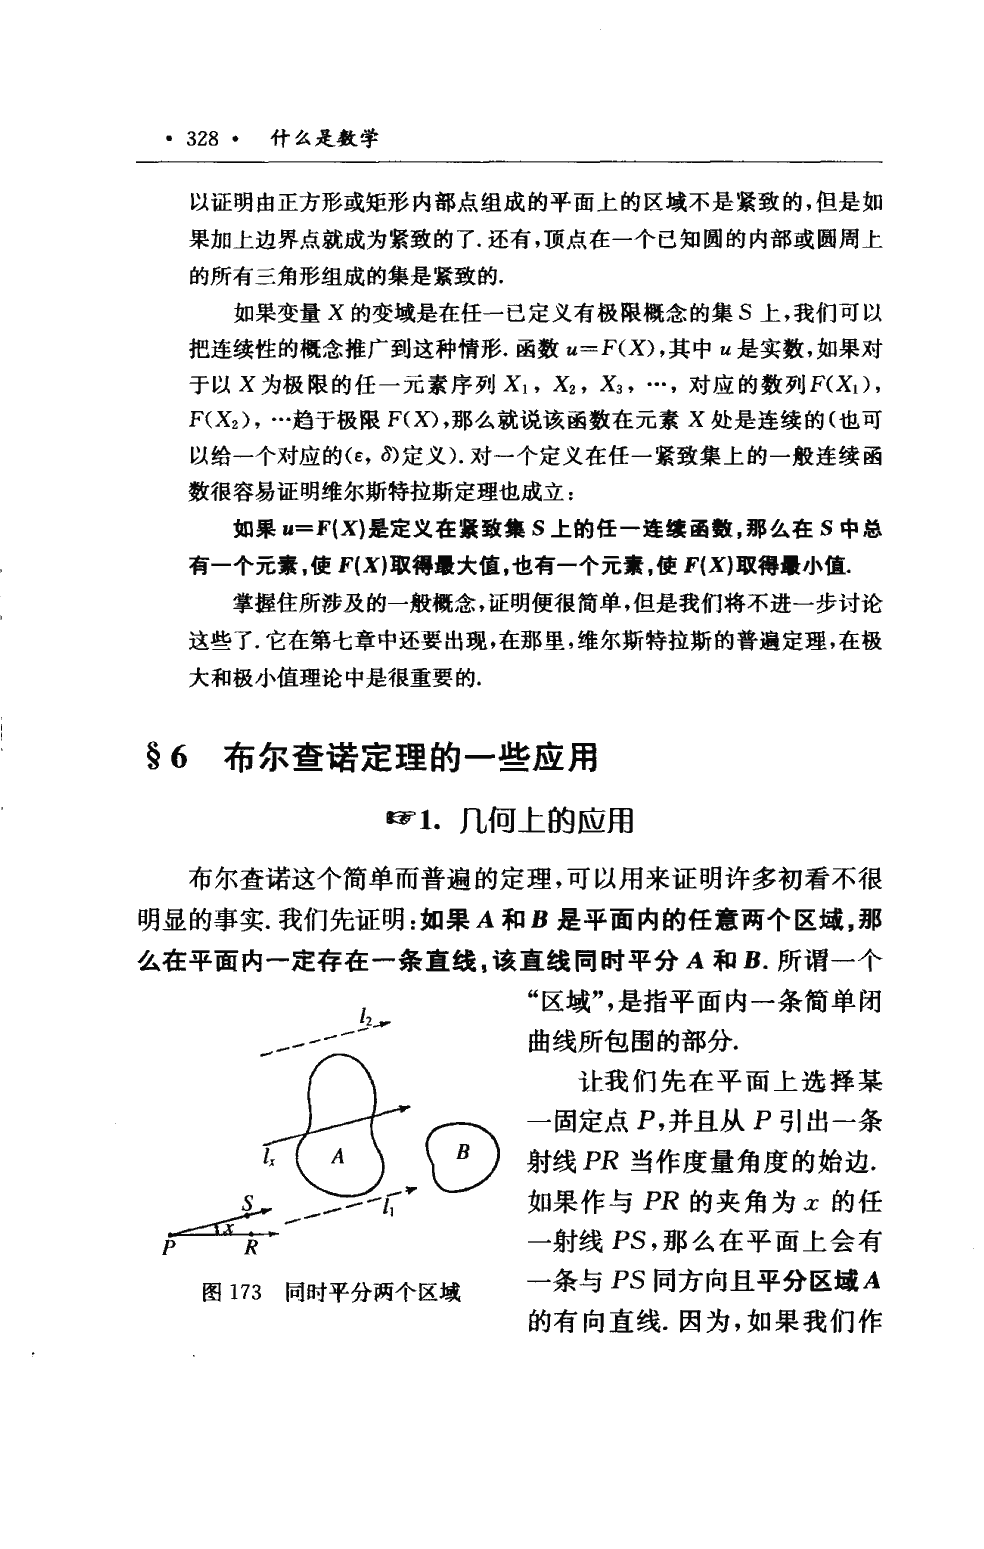
\includegraphics[height=1\textheight]{F:/life/2018AutumnTA/Exercises/4/intermediate-value-theorem1.png}
\end{center}
\end{figure}
\begin{figure}[H]
\begin{center}
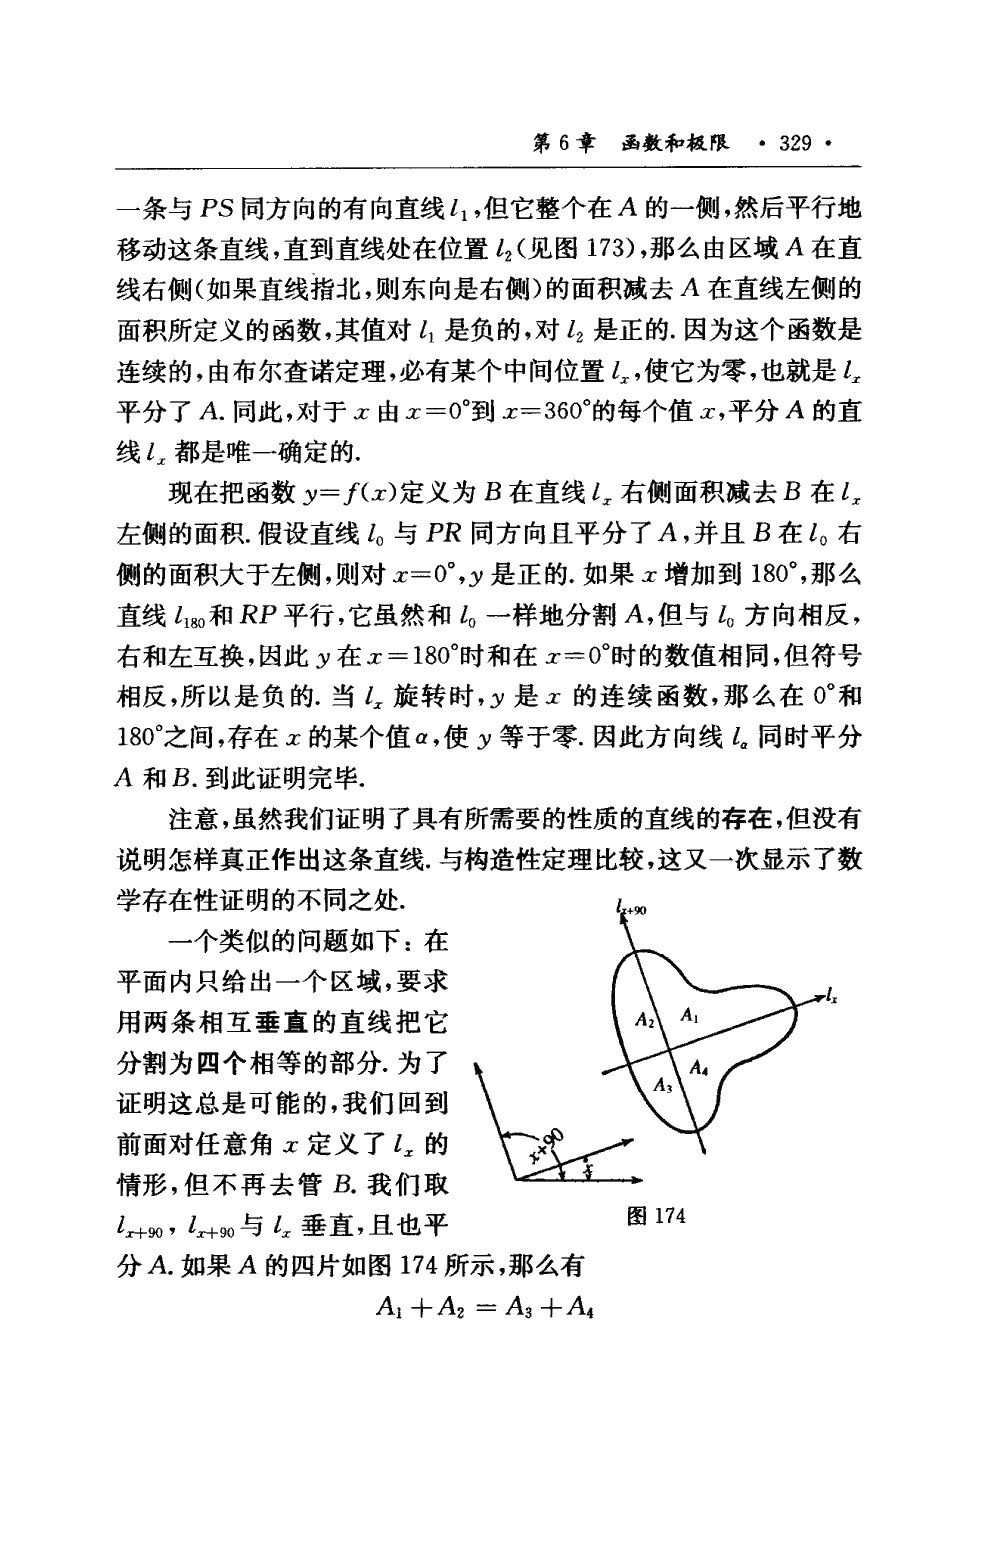
\includegraphics[height=1\textheight]{F:/life/2018AutumnTA/Exercises/4/intermediate-value-theorem2.png}
\end{center}
\end{figure}
\begin{figure}[H]
\begin{center}
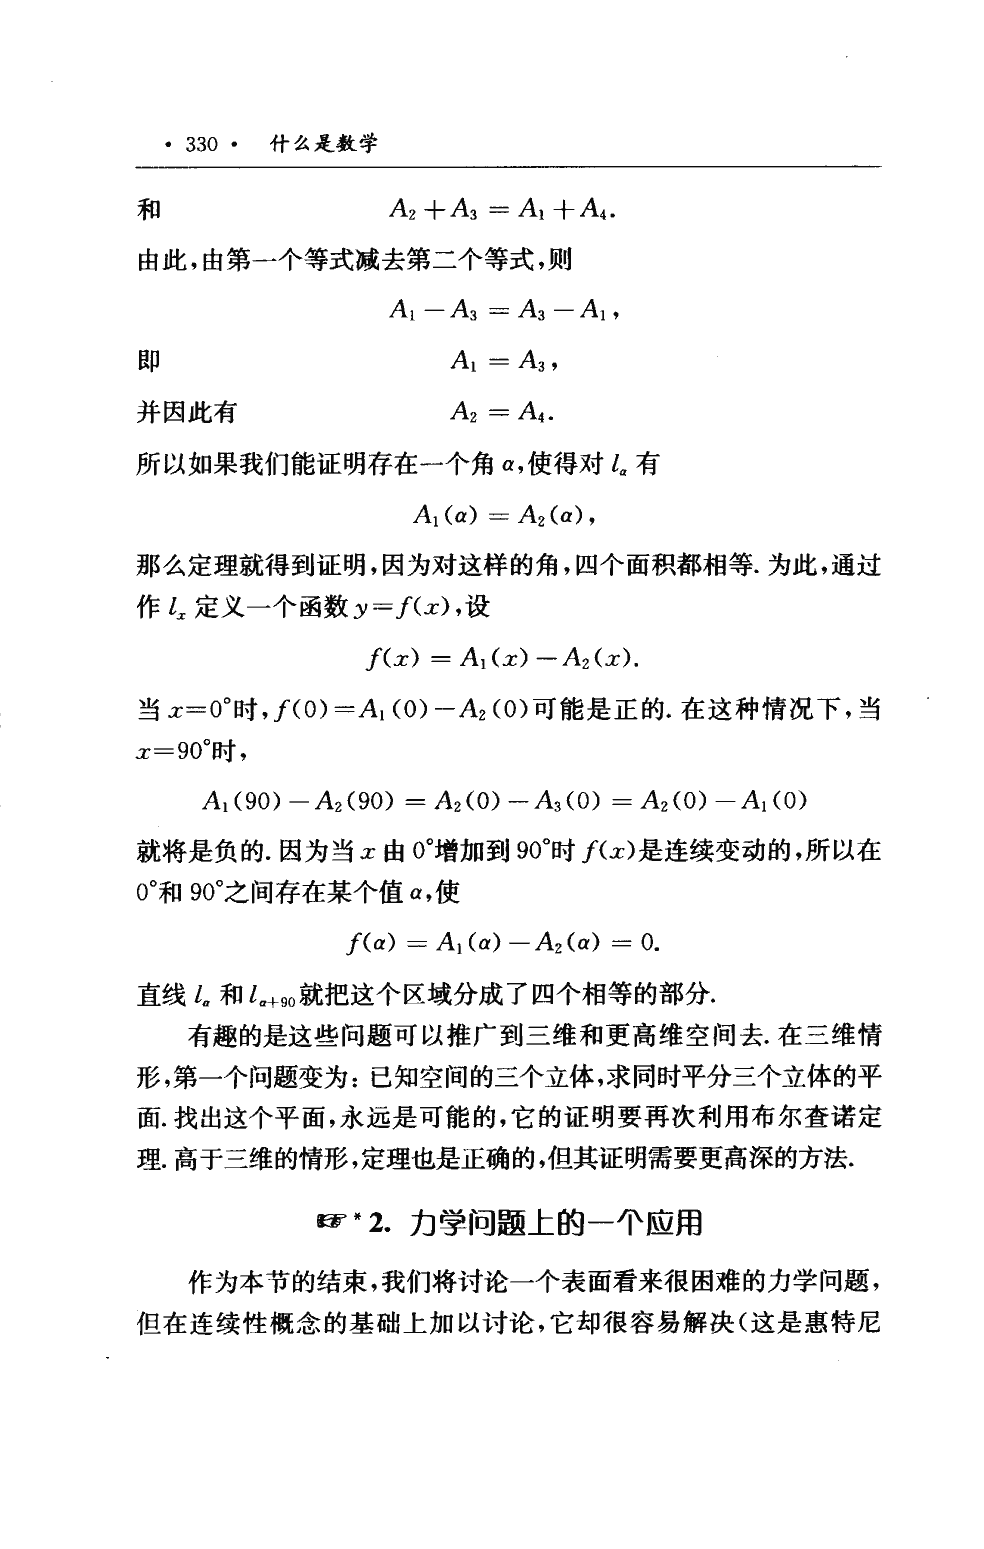
\includegraphics[height=1\textheight]{F:/life/2018AutumnTA/Exercises/4/intermediate-value-theorem3.png}
\end{center}
\end{figure}
\subsection{附录2}
\begin{figure}[H]
\begin{center}
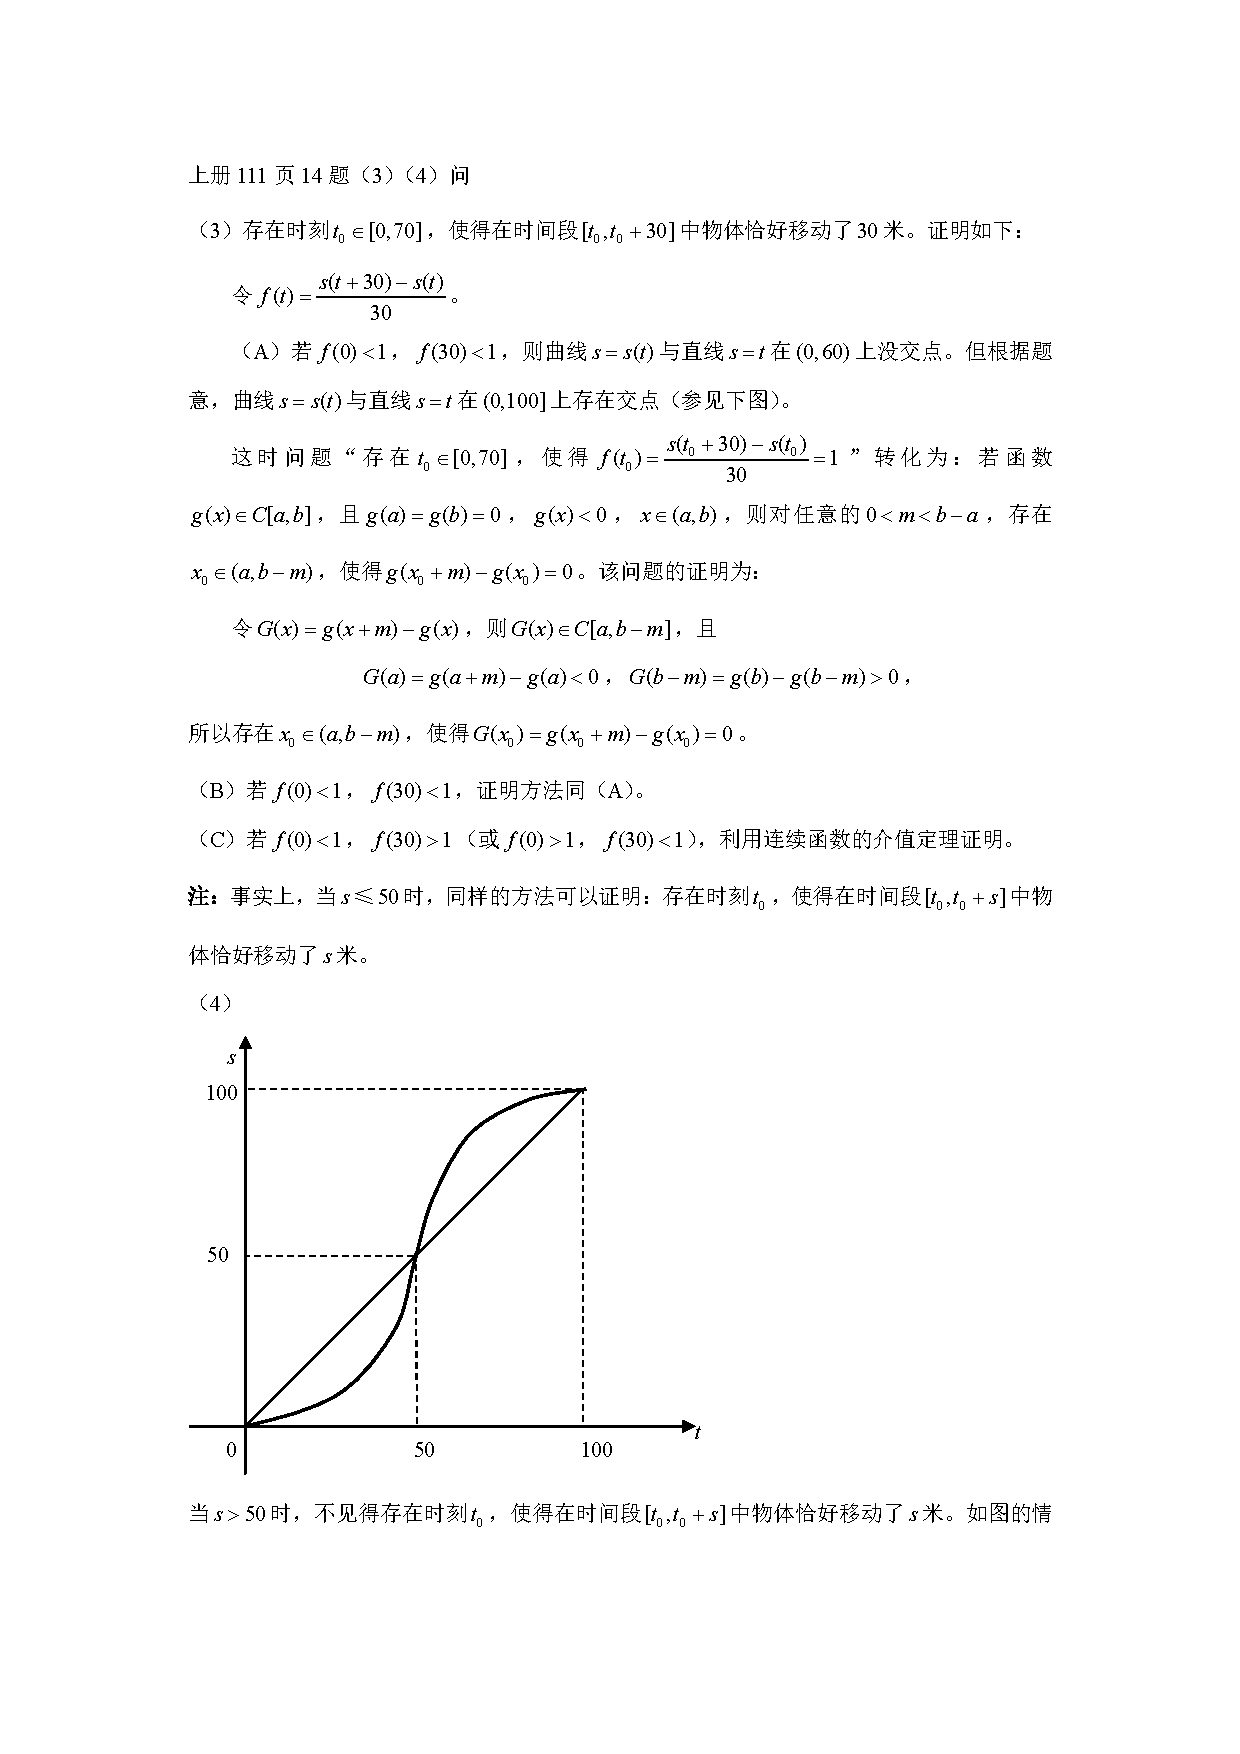
\includegraphics[height=1\textheight]{F:/life/2018AutumnTA/Exercises/4/Exercises.pdf}
\end{center}
\end{figure}
\begin{figure}[H]
\begin{center}
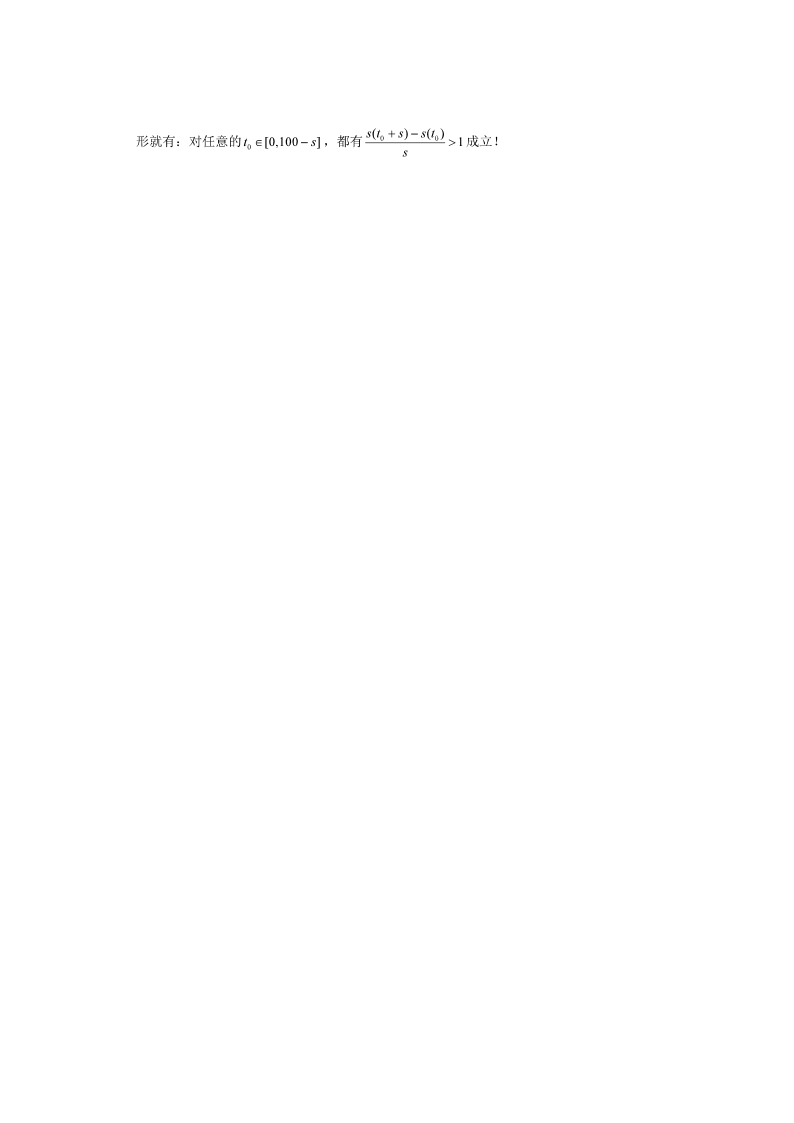
\includegraphics[height=1\textheight]{F:/life/2018AutumnTA/Exercises/4/Exercise2.png}
\end{center}
\end{figure}
\end{document}
\documentclass[12pt,UTF8]{ctexart}
\usepackage{ctex,amsmath,amssymb,geometry,fancyhdr,bm,amsfonts
,mathtools,extarrows,graphicx,url,enumerate,color} 
% 加入中文支持
\newcommand\Set[2]{%
\left\{#1\ \middle\vert\ #2 \right\}}
\geometry{a4paper,scale=0.80}
\pagestyle{fancy}
\rhead{习题4.1\&4.2\&4.3}
\lhead{基础习题课讲义}
\chead{微积分B(1)}
\begin{document}
\setcounter{section}{4}
\section{导数的概念、运算法则与若干特殊函数的求导方法}
\noindent
\subsection{知识结构}
\noindent第4章导数与微分
	\begin{enumerate}
		\item[4.1] 导数的概念
			\begin{enumerate}
				\item[4.1.1]导数
					\begin{itemize}
						\item运动物体的瞬时速度
						\item曲线的切线问题
							\begin{itemize}
								\item 切线
								\item 法线
							\end{itemize}
					\end{itemize}
				\item[4.1.2]基本初等函数的导数
					\begin{itemize}
						\item常数函数
						\item三角函数
						\item对数函数
						\item指数函数
					\end{itemize}
			\end{enumerate}
		\item[4.2]导数的运算法则
			\begin{enumerate}
				\item[4.2.1]导数的四则运算
					\begin{itemize}
						\item导数的四则运算法则
						\item复合函数求导法则
					\end{itemize}
				\item[4.2.2]反函数求导法则
			\end{enumerate}
		\item[4.3]若干特殊的求导方法
			\begin{enumerate}
				\item[4.3.1]对数求导法
				\item[4.3.2]参数式函数求导法
				\item[4.3.3]隐函数求导法
			\end{enumerate}
\end{enumerate}
\subsection{习题4.1解答}
\begin{enumerate}
\item 当物体温度高于室内温度时,物体就会逐渐冷却. 设物体温度$T$与时间$t$的关系为$T=T(t)$,试求物体在时刻$t$的冷却速率.

解:物体在时刻$t$的冷却速率为$T'(t)$.

\item 求等边三角形的面积关于其边长的变化率.

解:等边三角形的面积$S(a)=\frac12a^2\sin60^\circ$关于其边长$a$的变化率为$S'(a)=\frac{\sqrt3}2a$.


\item 求球体体积关于其半径的变化率. 并问:该变化率与这个球的表面积是什么关系?

解:球体体积$V(R)=\frac43\pi R^3$关于其半径$R$的变化率$V'(R)=4\pi R^2$,等于球的表面积.

\item 利用导数的定义求函数在指定点的导数:
\newline
(1)$f(x)=-5,x_0=2$;
\newline
(2)$f(x)=-2x+1,x_0=1$;
\newline
(3)$f(x)=\frac1x,x_0=-2$;
\newline
(4)$y=\cos x,x_1=0,x_2=\frac\pi2$;
\newline
(5)$f(x)=\sqrt x,x_0=4$;
\newline
(6)$f(x)=\begin{cases}
x^{\frac12},&x>1\\
\frac x2+\frac12,&x\leq1
\end{cases},x_0=1$.

解:(1)$f'(x_0)=\lim\limits_{x\rightarrow x_0}\frac{f(x)-f(x_0)}{x-x_0}=0$.

(2)$f'(x_0)=\lim\limits_{x\rightarrow x_0}\frac{f(x)-f(x_0)}{x-x_0}=-2$.

(3)$f'(x_0)=\lim\limits_{x\rightarrow x_0}\frac{f(x)-f(x_0)}{x-x_0}=\lim\limits_{x\rightarrow x_0}\frac{\frac1x-\frac1{x_0}}{x-x_0}=-\frac1{x_0^2}=-\frac14$.

(4)$y'(x_1)=\lim\limits_{x\rightarrow x_1}\frac{y(x)-y(x_1)}{x-x_1}=\lim\limits_{x\rightarrow x_1}\frac{\cos x-\cos x_1}{x-x_1}=\lim\limits_{x\rightarrow x_1}\frac{-2\sin{\frac{x+x_1}2}\sin{\frac{x-x_1}2}}{x-x_1}=-\sin x_1=0$;$y'(x_2)=-\sin x_2=-1$.

(5)$f'(x_0)=\lim\limits_{x\rightarrow x_0}\frac{f(x)-f(x_0)}{x-x_0}=\lim\limits_{x\rightarrow x_0}\frac{\sqrt x-\sqrt{x_0}}{x-x_0}=\frac1{2\sqrt{x_0}}=\frac14$.

(6)$f'_-(x_0)=\lim\limits_{x\rightarrow x_0-}\frac{f(x)-f(x_0)}{x-x_0}=\frac12,f'_+(x_0)=\lim\limits_{x\rightarrow x_0+}\frac{f(x)-f(x_0)}{x-x_0}=\frac1{2\sqrt{x_0}}=\frac12=f'_-(x_0)$,故$f'(x_0)=\frac12$.

\item 证明下列函数在其定义域内每一点处都可导,并求其导数:
\newline
(1)$f(x)=ax+b(a,b\text{为常数})$;
\newline
(2)$f(x)=\sqrt{x^3}$;
\newline
(3)$f(x)=\frac1{2x}$;
\newline
(4)$f(x)=\sin3x$;
\newline
(5)$f(x)=x^{\frac1n}(x\neq0,n\text{为正整数})$.

证明:(1)$f'(x)=\lim\limits_{\Delta x\rightarrow 0}\frac{f(x+\Delta x)-f(x)}{\Delta x}=a,x\in(-\infty,+\infty)$.

(2)$f'(x)=\lim\limits_{\Delta x\rightarrow 0}\frac{f(x+\Delta x)-f(x)}{\Delta x}=\lim\limits_{\Delta x\rightarrow 0}\frac{\sqrt{(x+\Delta x)^3}-\sqrt{x^3}}{\Delta x}=\lim\limits_{\Delta x\rightarrow 0}\frac{(x+\Delta x)^3-x^3}{\Delta x[\sqrt{(x+\Delta x)^3}+\sqrt{x^3}]}=\frac32\sqrt x,x>0,f'_+(0)=\lim\limits_{\Delta x\rightarrow 0+}\frac{f(\Delta x)-f(0)}{\Delta x}=\lim\limits_{\Delta x\rightarrow 0+}\frac{\sqrt{\Delta x^3}-0}{\Delta x}=0$.

(3)$f'(x)=\lim\limits_{\Delta x\rightarrow 0}\frac{f(x+\Delta x)-f(x)}{\Delta x}=\lim\limits_{\Delta x\rightarrow 0}\frac{\frac1{2(x+\Delta x)}-\frac1{2x}}{\Delta x}=\frac1{2x},x\neq0$.

(4)$f'(x)=\lim\limits_{\Delta x\rightarrow 0}\frac{f(x+\Delta x)-f(x)}{\Delta x}=\lim\limits_{\Delta x\rightarrow 0}\frac{\sin3(x+\Delta x)-\sin 3x}{\Delta x}=\lim\limits_{\Delta x\rightarrow 0}\frac{2\cos\frac{6x+3\Delta x}2\sin\frac{3\Delta x}2}{\Delta x}=3\cos3x,x\in(-\infty,+\infty)$.

(5)当$n=1$时,$f'(x)=\lim\limits_{\Delta x\rightarrow 0}\frac{(x+\Delta x)-x}{\Delta x}=1,x\neq0$

当$n\geq2$时,$f'(x)=\lim\limits_{\Delta x\rightarrow 0}\frac{f(x+\Delta x)-f(x)}{\Delta x}=\lim\limits_{\Delta x\rightarrow 0}\frac{(x+\Delta x)^{\frac1n}-x^{\frac1n}}{\Delta x}
\\=\lim\limits_{\Delta x\rightarrow 0}\frac{(x+\Delta x)-x}{\Delta x[(x+\Delta x)^{\frac{n-1}n}+(x+\Delta x)^{\frac{n-2}n}x^{\frac1n}+\cdots+x^{\frac{n-1}n}]}=\lim\limits_{\Delta x\rightarrow 0}\frac{1}{(x+\Delta x)^{\frac{n-1}n}+(x+\Delta x)^{\frac{n-2}n}x^{\frac1n}+\cdots+x^{\frac{n-1}n}}
\\=\frac{1}{(x)^{\frac{n-1}n}+(x)^{\frac{n-2}n}x^{\frac1n}+\cdots+x^{\frac{n-1}n}}=\frac1{nx^{\frac{n-1}n}}=\frac1nx^{\frac1n-1}$

当$n$为奇数时,$x\neq0$,导函数与原函数的定义域相同,当$n$为偶数时,$x>0$,导函数与原函数的定义域也相同,故函数$f(x)$在其定义域内每一点处都可导.

两种情况合并可得$f'(x)=\frac1nx^{\frac1n-1}$,当$n$为奇数时,$x\neq0$,当$n$为偶数时,$x>0$.
\item研究下列分段函数在分段点处的可导性,若可导,求出导数值:
\newline
(1)$y=|x-3|$,在点$x=3$;
\newline
(2)$y=\begin{cases}
x,&x<0\\
\ln(1+x),&x\geq0
\end{cases}$,在点$x=0$;
\newline
(3)$f(x)=|x|+2x$,在点$x=0$;
\newline
(4)$g(x)=\begin{cases}
3x^2+4x,&x<0\\
x^2-1,&x\geq0
\end{cases}$,在点$x=0$;
\newline
(5)$y(x)=\begin{cases}
x\sin\frac1x,&x\neq0\\
0,&x=0
\end{cases}$,在点$x=0$;
\newline
(6)$y(x)=\begin{cases}
\frac1{1+e^{1/x}},&x\neq0\\
0,&x=0
\end{cases}$,在点$x=0$.

解:(1)$y'_+(3)=\lim\limits_{\Delta x\rightarrow0+}\frac{y(3+\Delta x)-y(3)}{\Delta x}=\lim\limits_{\Delta x\rightarrow0+}\frac{\Delta x-0}{\Delta x}=1,y'_-(3)=\lim\limits_{\Delta x\rightarrow0-}\frac{y(3+\Delta x)-y(3)}{\Delta x}=\lim\limits_{\Delta x\rightarrow0-}\frac{-\Delta x-0}{\Delta x}=-1\neq y'_+(3)$,故原函数在点$x=3$处不可导.

(2)$y'_+(0)=\lim\limits_{\Delta x\rightarrow0+}\frac{y(0+\Delta x)-y(0)}{\Delta x}=\lim\limits_{\Delta x\rightarrow0+}\frac{\ln(1+\Delta x)-0}{\Delta x}=1,y'_-(0)=\lim\limits_{\Delta x\rightarrow0-}\frac{y(0+\Delta x)-y(0)}{\Delta x}=\lim\limits_{\Delta x\rightarrow0-}\frac{\Delta x-0}{\Delta x}=1=y'_+(0)$,故原函数在点$x=0$处可导,导数为1.

(3)$f'_+(0)=\lim\limits_{\Delta x\rightarrow0+}\frac{f(0+\Delta x)-f(0)}{\Delta x}=\lim\limits_{\Delta x\rightarrow0+}\frac{\Delta x+2\Delta x-0}{\Delta x}=3,f'_-(0)=\lim\limits_{\Delta x\rightarrow0-}\frac{f(0+\Delta x)-f(0)}{\Delta x}=\lim\limits_{\Delta x\rightarrow0-}\frac{-\Delta x+2\Delta x-0}{\Delta x}=1\neq f'_+(0)$,故原函数在$x=0$处不可导.

(4)$g(0+0)=\lim\limits_{\Delta x\rightarrow0+}g(x)=-1,g(0-0)=\lim\limits_{\Delta x\rightarrow0-}g(x)=0\neq g(0+0)$,原函数在$x=0$处不连续,故不可导.

(5)$\lim\limits_{\Delta x\rightarrow0}\frac{y(0+\Delta x)-y(0)}{\Delta x}=\lim\limits_{\Delta x\rightarrow0}\sin\frac1{\Delta x}$,该极限不存在,故原函数在$x=0$处不可导.

(6)$y(0+0)=\lim\limits_{\Delta x\rightarrow0+}\frac1{1+e^{1/x}}=0,y(0-0)=\lim\limits_{\Delta x\rightarrow0-}\frac1{1+e^{1/x}}=1\neq y(0+0)$,原函数在$x=0$处不连续,故不可导.
\item设函数$f(x)$在点$x_0$处可导,求$\lim\limits_{n\rightarrow\infty}n[f(x_0+\frac1n)-f(x_0)]$.

解:$\because f(x)$在点$x_0$处可导

$\therefore f'(x_0)=\lim\limits_{\Delta x\rightarrow0}\frac{f(x_0+\Delta x)-f(x_0)}{\Delta x}$

记$g(t)=\frac{f(x_0+t)-f(x_0)}{t}$,则$\lim\limits_{t\rightarrow0}g(t)=f'(x_0)$

$\because$数列$a_n=\frac1n,n=1,2,\cdots$满足$\lim\limits_{n\rightarrow\infty}a_n=0$,且$a_n\neq0$

$\therefore\lim\limits_{n\rightarrow\infty}n[f(x_0+\frac1n)-f(x_0)]=\lim\limits_{n\rightarrow\infty}g(a_n)=f'(x_0)$.

\item设函数$f(x)$在点$x_0$处可导,则
\[
\lim\limits_{h\rightarrow0}\frac{f(x_0+h)-f(x_0-h)}{2h}=f'(x_0).
\]
反之,若此极限存在,问:$f(x)$在点$x_0$处是否可导?

解:若$f(x)$在点$x_0$处可导,则$\lim\limits_{h\rightarrow0}\frac{f(x_0+h)-f(x_0-h)}{2h}=\lim\limits_{h\rightarrow0}\frac12[\frac{f(x_0+h)-f(x_0)}h+\frac{f(x_0)-f(x_0-h)}h]=\frac12[2f'(x_0)]=f'(x_0)$.

可能不正确的做法:若$f(x)$在点$x_0$处可导,则$f'(x_0)=\lim\limits_{\Delta x\rightarrow0}\frac{f(x_0+\Delta x)-f(x_0)}{\Delta x}\xlongequal{t=x_0+\frac{\Delta x}2}\lim\limits_{\Delta x\rightarrow0}\frac{f(t+\frac{\Delta x}2)-f(t-\frac{\Delta x}2)}{2\frac{\Delta x}2}=\lim\limits_{h\rightarrow0}\frac{f(t+h)-f(t-h)}{2h}\neq\lim\limits_{h\rightarrow0}\frac{f(x_0+h)-f(x_0-h)}{2h}$.

反之,若此极限存在,则函数$f(x)$在点$x_0$处不一定可导. 如取$f(x)=|x|$,在$x_0=0$处,$\lim\limits_{h\rightarrow0}\frac{f(x_0+h)-f(x_0-h)}{2h}=\lim\limits_{h\rightarrow0}\frac{|0+h|-|0-h|}{2h}=0$,但$f(x)$在$x=0$处的导数不存在.

\item假设$f'(a)$存在,试求:$\lim\limits_{h\rightarrow0}\frac{f(a-h)-f(a)}{h}$.

解:$\lim\limits_{h\rightarrow0}\frac{f(a-h)-f(a)}{h}=-\lim\limits_{h\rightarrow0}\frac{f(a-h)-f(a)}{-h}=-\lim\limits_{\Delta x\rightarrow0}\frac{f(a+\Delta x)-f(a)}{\Delta x}=-f'(a)$.

\item假设$f(x)$在点$a$处可导,并令
\[
g(x)=\begin{cases}
\frac{f(x)-f(a)}{x-a},&x\neq a\\
f'(a),&x=a
\end{cases}
\]
试证:$g(x)$在$a$处连续.

证明:$\lim\limits_{x\rightarrow a}g(x)=\lim\limits_{x\rightarrow a}\frac{f(x)-f(a)}{x-a}=f'(a)=g(a)$,故$g(x)$在$a$处连续.

\item设$f(x)=\begin{cases}
x^2,&x\leq x_0\\
ax+b,&x>x_0
\end{cases}$,为了使函数$f(x)$在点$x_0$处可导,应当如何选取系数$a$和$b$?

解:$\because f(x)$在点$x_0$处可导

$\therefore f(x)$在点$x_0$处连续

$\therefore f(x_0+0)=\lim\limits_{x\rightarrow x_0+}f(x)=ax_0+b=f(x_0-0)=x_0^2$

$f'_-(x_0)=\lim\limits_{x\rightarrow x_0-}\frac{f(x)-f(x_0)}{x-x_0}=\lim\limits_{x\rightarrow x_0-}\frac{x^2-x_0^2}{x-x_0}=2x_0,f'_+(x_0)=\lim\limits_{x\rightarrow x_0+}\frac{f(x)-f(x_0)}{x-x_0}=\lim\limits_{x\rightarrow x_0+}\frac{ax+b-x_0^2}{x-x_0}=\lim\limits_{x\rightarrow x_0+}\frac{ax+b-ax+b}{x-x_0}=a$

由$f(x)$在点$x_0$处可导又可知$f'_-(x_0)=f'_+(x_0)$,故$a=2x_0,b=x_0^2-ax_0=-x_0^2$.

\item证明:
\newline
(1)可导偶函数的导函数为奇函数;
\newline
(2)可导奇函数的导函数为偶函数;
\newline
(3)可导周期函数,其导函数为具有相同周期的周期函数.

证明:(1)记$f(x)$为可导偶函数,则$f(x)=f(-x)$

$f'(x)=\lim\limits_{\Delta x\rightarrow0}\frac{f(x+\Delta x)-f(x)}{\Delta x}=-\lim\limits_{\Delta x\rightarrow0}\frac{f(-x-\Delta x)-f(-x)}{-\Delta x}=-f'(-x)$,故导函数$f'(x)$为奇函数.

(2)记$f(x)$为可导奇函数,则$f(x)=-f(-x)$

$f'(x)=\lim\limits_{\Delta x\rightarrow0}\frac{f(x+\Delta x)-f(x)}{\Delta x}=-\lim\limits_{\Delta x\rightarrow0}\frac{-f(-x-\Delta x)+f(-x)}{-\Delta x}=\lim\limits_{\Delta x\rightarrow0}\frac{f(-x-\Delta x)-f(-x)}{-\Delta x}=f'(-x)$,故导函数$f'(x)$为偶函数.

(3)记$f(x)$为可导周期函数,$T$为其周期,则$f(x+T)=f(x)$

$f'(x+T)=\lim\limits_{\Delta x\rightarrow0}\frac{f(x+T+\Delta x)-f(x+T)}{\Delta x}=\lim\limits_{\Delta x\rightarrow0}\frac{f(x+\Delta x)-f(x)}{\Delta x}=f'(x)$,故导函数$f'(x)$为具有相同周期的周期函数.
\end{enumerate}
\subsection{习题4.2解答}
\begin{enumerate}
\item求下列各函数的导数:
\newline
(1)$f(x)=x^3-4x+5$;
\newline
(2)$y=2x^4-3x^3+x-\frac1{3x^2}+\frac7{x^3}$;
\newline
(3)$y=\frac x3+\frac3x+2\sqrt x$;
\newline
(4)$f(x)=7x^2+\cos x-\ln x$;
\newline
(5)$f(x)=\sqrt x\cos x$;
\newline
(6)$g(x)=e^x\sin x$;
\newline
(7)$y=\sqrt{x^2+1}\cot x$;
\newline
(8)$f(t)=(t+t^2)^2$;
\newline
(9)$y=\frac{\tan x}x$;
\newline
(10)$y=\frac x{1-\cos x}$;
\newline
(11)$y=\frac{1+\ln x}{1-\ln x}$;
\newline
(12)$y=\frac{x}{\sin^2x}$;
\newline
(13)$g(x)=\frac{\arcsin x}{\sqrt x}$;
\newline
(14)$y=\frac{\ln x}{\cos x}$;
\newline
(15)$f(x)=\sqrt x\sec x$;
\newline
(16)$y=\sec x\tan x$;
\newline
(17)$y=(\sqrt x+1)\arctan x$;
\newline
(18)$g(z)=\frac{\csc z}{z^2}$;
\newline
(19)$y=\frac1x+\frac1{\sqrt x}-\frac1{\sqrt[3]x}$;
\newline
(20)$y=\frac{\sin x-x\cos x}{\cos x+x\cos x}$.

解:(1)$f'(x)=3x^2-4$.

(2)$y'=8x^3-9x^2+1+\frac2{3x^3}-\frac{21}{x^4}$.

(3)$y'=\frac13-\frac3{x^2}+\frac1{\sqrt x}$.

(4)$f'(x)=14x-\sin x-\frac1x$.

(5)$f'(x)=\frac1{2\sqrt x}\cos x-\sqrt x\sin x$.

(6)$g'(x)=e^x\sin x+e^x\cos x$.

(7)$y'=\frac{2x}{2\sqrt{x^2+1}}\cot x-\sqrt{x^2+1}\csc^2x=\frac{x\cot x-(x^2+1)\csc^2x}{\sqrt{x^2+1}}$.

(8)$f'(t)=2(t+t^2)(1+2t)$.

(9)$y'=\frac{x\sec^2x-\tan x}{x^2}$.

(10)$y'=\frac{1-\cos x-x\sin x}{(1-\cos x)^2}$.

(11)$y'=\frac{\frac1x(1-\ln x)+(1+\ln x)\frac1x}{(1-\ln x)^2}=\frac2{x(1-\ln x)^2}$.

(12)$y'=\frac{\sin^2x-x2\sin x\cos x}{\sin^4x}=\frac{\sin x-2x\cos x}{\sin^3x}$.

(13)$g'(x)=\frac{\frac1{\sqrt{1-x^2}}\sqrt x-\frac1{2\sqrt x}\arcsin x}{x}=\frac1{\sqrt x\sqrt{1-x^2}}-\frac1{2x\sqrt x}\arcsin x$.

(14)$y'=\frac{\frac1x\cos x+\ln x\sin x}{\cos^2x}=\frac{\cos x+x\ln x\sin x}{x\cos^2x}$.

(15)$f'(x)=\frac1{2\sqrt x}\sec x+\sqrt x\sec x\tan x$

(16)$y'=\sec x\tan^2x+\sec^3x$.

(17)$y'=\frac1{2\sqrt x}\arctan x+\frac{\sqrt x+1}{1+x^2}$.

(18)$g'(z)=\frac{-z^2\csc z\cot z-2z\csc z}{z^4}=\frac{-z\csc z\cot z-2\csc z}{z^3}$.

(19)$y'=-\frac1{x^2}-\frac1{2\sqrt{x^3}}+\frac1{3\sqrt[3]{x^4}}$.

(20)$y'=\frac{(\cos x-\cos x+x\sin x)(\cos x+x\sin x)-(\sin x-x\cos x)(-\sin x+\sin x+x\cos x)}{(\cos x+x\sin x)^2}
\\=\frac{x\sin x(\cos x+x\sin x)-(\sin x-x\cos x)x\cos x}{(\cos x+x\sin x)^2}=\frac{x^2}{(\cos x+x\sin x)^2}$.

\item设$y=2+x-x^2$,求$y'(0),y'(\frac12),y'(1),y'(-10)$.

解:$\because y'(x)=1-2x$

$\therefore y'(0)=1,y'(\frac12)=0,y'(1)=-1,y'(-10)=21$.

\item求出下列各题中的$a$值:
\newline
(1)$f(x)=-2x^2,f'(a)=f(4)$;
\newline
(2)$f(x)=\frac1x,f'(a)=-\frac19$;
\newline
(3)$f(x)=\sin x,f'(a)=\frac{\sqrt3}2$.

解:(1)$f'(x)=-4x,f'(a)=f(4)\Rightarrow -4a=-32$,故$a=8$.

(2)$f'(x)=-\frac1{x^2},f'(a)=-\frac19\Rightarrow -\frac1{a^2}=-\frac19$,故$a=\pm3$.

(3)$f'(x)=\cos x,f'(a)=\frac{\sqrt3}2\Rightarrow\cos a=\frac{\sqrt3}2$,故$a=2k\pi\pm\frac\pi6,k\in\mathbb Z$.

\item求下列函数的导数:
\newline
(1)$y=2\sin3x$;
\newline
(2)$y=xe^{-x^2}$;
\newline
(3)$y=\ln(1-2t)$;
\newline
(4)$y=\ln\ln x$;
\newline
(5)$y=\sqrt{1+2\tan x}$;
\newline
(6)$y=\ln(\cos x)$;
\newline
(7)$y=\arcsin\frac1x$;
\newline
(8)$y=\arccos\frac{2x-1}{\sqrt3}$;
\newline
(9)$y=2^{\ln\frac1x}$;
\newline
(10)$y=x\sqrt{1-x^2}$;
\newline
(11)$y=\sqrt{2-x}\sqrt[3]{3+x}$;
\newline
(12)$y=\frac{x}{\sqrt{a^2-x^2}}$;
\newline
(13)$y=\sqrt[3]{\frac{1-x}{1+x}}$;
\newline
(14)$y=\ln(x+\sqrt{1+x^2})$;
\newline
(15)$y=\sqrt{x-\sqrt x}$;
\newline
(16)$y=\frac{\sin^2x}{\sin(x^2)}$;
\newline
(17)$y=e^{-3x}\sin2x$;
\newline
(18)$y=\lg^3x^2$;
\newline
(19)$y=\frac x2\sqrt{x^2+a^2}+\frac{a^2}2\ln(x+\sqrt{x^2+a^2})$;
\newline
(20)$y=\ln\tan(\frac x2+\frac\pi4)$;
\newline
(21)$y=\arcsin(\sin^2x)$;
\newline
(22)$y=\arccos\sqrt{1-x^2}$;
\newline
(23)$y=\arccos\frac1{\sqrt x}$;
\newline
(24)$y=\frac x2\sqrt{a^2-x^2}+\frac{a^2}2\arcsin\frac xa$;
\newline
(25)$y=\ln(\sqrt{1+x}-\sqrt x)$.

解:(1)$y'=6\cos3x$.

(2)$y'=e^{-x^2}+xe^{-x^2}(-2x)=e^{-x^2}(1-2x^2)$.

(3)$y'=\frac1{1-2t}(-2)=\frac2{2t-1}$.

(4)$y'=\frac1{\ln x}\frac1x=\frac1{x\ln x}$.

(5)$y'=\frac{2\sec^2x}{2\sqrt{1+\tan x}}=\frac{\sec^2x}{\sqrt{1+\tan x}}$.

(6)$y'=\frac{-\sin x}{\cos x}=-\tan x$.

(7)$y'=\frac1{\sqrt{1-\frac1{x^2}}}\frac{-1}{x^2}=\frac{-1}{\sqrt{x^4-x^2}}$.

(8)$y'=\frac{-1}{\sqrt{1-(\frac{2x-1}{\sqrt3})^2}}\frac2{\sqrt3}=\frac{-2}{\sqrt{2+4x-4x^2}}$.

(9)$y'=2^{\ln\frac1x}\ln2\cdot\frac1{\frac1x}\frac{-1}{x^2}=-2^{\ln \frac1x}\frac{\ln2}{x}$.

(10)$y'=\sqrt{1-x^2}+x\frac{-2x}{2\sqrt{1-x^2}}=\frac{1-2x^2}{\sqrt{1-x^2}}$.

(11)$y'=\frac{-1}{2\sqrt{2-x}}\sqrt[3]{3+x}+\sqrt{2-x}\frac1{3\sqrt{(3+x)^2}}=\frac{-\sqrt[3]{3+x}}{2\sqrt{2-x}}+\frac{\sqrt{2-x}}{3\sqrt{(3+x)^2}}$.

(12)$y'=\frac{\sqrt{a^2-x^2}-x\frac{-2x}{2\sqrt{a^2-x^2}}}{a^2-x^2}=\frac{a^2}{(a^2-x^2)^\frac32}$.

(13)$y'=\frac13\sqrt[3]{(\frac{1+x}{1-x})^2}\frac{-(1+x)-(1-x)}{(1+x)^2}=-\frac23\frac1{(1+x)^2}\sqrt[3]{(\frac{1+x}{1-x})^2}$.

(14)$y'=\frac1{x+\sqrt{1+x^2}}(1+\frac{2x}{2\sqrt{1+x^2}})=\frac1{\sqrt{1+x^2}}$.

(15)$y'=\frac1{2\sqrt{x-\sqrt x}}(1+\frac{-1}{2\sqrt x})=\frac{2\sqrt x-1}{4\sqrt{x^2-x\sqrt{x}}}$.

(16)$y'=\frac{2\sin x\cos x\sin(x^2)-2x\sin^2x\cos(x^2)}{\sin^2(x^2)}=\frac{\sin2x\sin(x^2)-2x\sin^2x\cos(x^2)}{\sin^2(x^2)}$.

(17)$y'=-3e^{-3x}\sin2x+2e^{-3x}\cos2x=e^{-3x}(-3\sin2x+2\cos2x)$.

(18)$y'=(3\lg^2x^2)\frac1{x^2\ln10}2x=6\frac{\lg^2x^2}{x\ln10}$.

(19)$y'=\frac12\sqrt{x^2+a^2}+\frac x2\frac{2x}{2\sqrt{x^2+a^2}}+\frac{a^2}2\frac{1+\frac{2x}{2\sqrt{x^2+a^2}}}{x+\sqrt{x^2+a^2}}=\sqrt{x^2+a^2}$.

(20)$y'=\frac12\frac1{\tan(\frac x2+\frac\pi4)}\sec^2(\frac x2+\frac\pi4)=\frac{\sec^2(\frac x2+\frac\pi4)}{2\tan(\frac x2+\frac\pi4)}=\sec x$.

(21)$y'=\frac{2\sin x\cos x}{\sqrt{1-\sin^4x}}=\frac{\sin2x}{\sqrt{1-\sin^4x}}$.

(22)$y'=\frac{-1}{\sqrt{1-1+x^2}}\frac{-2x}{2\sqrt{1-x^2}}=\frac x{|x|\sqrt{1-x^2}}$.

(23)$y'=\frac{-1}{\sqrt{1-\frac1x}}\frac{-1}{2x\sqrt x}=\frac1{2x\sqrt{x-1}}$.

(24)$y'=\frac12\sqrt{a^2-x^2}+\frac x2\frac{-2x}{2\sqrt{a^2-x^2}}+\frac{a^2}2\frac1{a\sqrt{1-\frac{x^2}{a^2}}}=\frac{a^2-2x^2}{2\sqrt{a^2-x^2}}+\frac a{2\sqrt{1-\frac{x^2}{a^2}}}$.

(25)$y'=\frac{\frac1{2\sqrt{1+x}}-\frac1{2\sqrt x}}{\sqrt{1+x}-\sqrt x}=-\frac1{2\sqrt{1+x}\sqrt x}$.

\item设$f$为可导函数,求下列各函数的导数:
\newline
(1)$f(\sqrt{1-x^2})$;
\newline
(2)$f(\frac1x)$;
\newline
(3)$f(\ln x)$;
\newline
(4)$f(e^x)e^{f(x)}$;
\newline
(5)$f(f(f(x)))$;
\newline
(6)$\sqrt{f^2(x)}$.

解:(1)$(f(\sqrt{1-x^2}))'=f'(\sqrt{1-x^2})\frac{-2x}{2\sqrt{1-x^2}}=f'(\sqrt{1-x^2})\frac{-x}{\sqrt{1-x^2}}$.

(2)$(f(\frac1x))'=\frac{-1}{x^2}f'(\frac1x)$.

(3)$(f(\ln x))'=f'(\ln x)\frac1x$.

(4)$(f(e^x)e^{f(x)})'=f'(e^x)e^xe^{f(x)}+f(e^x)e^{f(x)}f'(x)=e^{f(x)}(f'(e^x)e^x+f(e^x)f'(x))$.

(5)$(f(f(f(x))))'=f'(f(f(x)))f'(f(x))f'(x)$.

(6)$(\sqrt{f^2(x)})'=\frac1{2\sqrt{f^2(x)}}2f(x)f'(x)=\frac{f(x)f'(x)}{\sqrt{f^2(x)}}$.
\end{enumerate}
\subsection{习题4.3解答}
\begin{enumerate}
\item 利用对数求导法求下列函数的导数:
\newline
(1)$y=\frac{x^2}{1-x}\sqrt[3]{\frac{x+1}{1+x+x^2}}$;
\newline
(2)$y=(x-a_1)^{a_1}(x-a_2)^{a_2}\cdots(x-a_n)^{a_n}$;
\newline
(3)$y=x^{\sin x}$;
\newline
(4)$y=(1+\frac1x)^{\frac1x}$;
\newline
(5)$y=\sqrt[x]x(x>0)$;
\newline
(6)$y=x+x^x+x^{x^x}(x>0)$.

解:(1)$(\ln y)'=[2\ln x-\ln(1-x)+\frac13\ln(1+x)-\frac13\ln(1+x+x^2)]'=\frac2x+\frac1{1-x}+\frac13\frac1{1+x}-\frac13\frac{1+2x}{1+x+x^2}$

$y'=y(\ln y)'=\frac{x^2}{1-x}\sqrt[3]{\frac{x+1}{1+x+x^2}}[\frac2x+\frac1{1-x}+\frac13\frac1{1+x}-\frac13\frac{1+2x}{1+x+x^2}]$.

(2)$(\ln y)'=[a_1\ln(x-a_1)+a_2\ln(x-a_2)+\cdots+a_n\ln(x-a_n)]'=\frac{a_1}{x-a_1}+\frac{a_2}{x-a_2}+\cdots+\frac{a_n}{x-a_n}$

$y'=y(\ln y)'=(x-a_1)^{a_1}(x-a_2)^{a_2}\cdots(x-a_n)^{a_n}(\frac{a_1}{x-a_1}+\frac{a_2}{x-a_2}+\cdots+\frac{a_n}{x-a_n})$.

(3)$(\ln y)'=(\sin x\ln x)'=\cos x\ln x+\frac{\sin x}x$

$y'=y(\ln y)'=y=x^{\sin x}(\cos x\ln x+\frac{\sin x}x)$.

(4)$(\ln y)'=[x\ln(1+\frac1x)]'=\ln(1+\frac1x)+\frac{x}{1+\frac1x}\frac{-1}{x^2}=\ln(1+\frac1x)-\frac1{1+x}$

$y'=y(\ln y)'=(1+\frac1x)^{\frac1x}[\ln(1+\frac1x)-\frac1{1+x}]$.

(5)$(\ln y)'=(\frac1x\ln x)'=\frac{-1}{x^2}\ln x+\frac1{x^2}=\frac1{x^2}(1-\ln x)$

$y'=y(\ln y)'=\frac{\sqrt[x]x}{x^2}(1-\ln x)$.

(6)记$y_1=x,y_2=x^x,y_3=x^{x^x}$

$y_1'=1$

$y_2'=y_2(\ln y_2)'=x^x(\ln x+1)$

$y_3'=y_3(\ln y_3)'$

$\because (\ln y_3)'=(\ln y_3)[\ln(\ln y_3)]'=(x^x\ln x)[x\ln x+\ln(\ln x)]'=(x^x\ln x)[\ln x+1+\frac1{\ln x}\frac1x]=(\ln x+1)(x^x\ln x)+x^{x-1}$

$\therefore y_3'=y_3(\ln y_3)'=x^{x^x}[(\ln x+1)x^x\ln x+x^{x-1}]$

$\therefore y'=y_1'+y_2'+y_3'=1+x^x(\ln x+1)+x^{x^x}[(\ln x+1)x^x\ln x+x^{x-1}]$.

\item求导数$\frac{\mathrm d y}{\mathrm d x}$:
\newline
(1)$\begin{cases}
x=\sin^2t\\
y=\cos^2t
\end{cases}$;
\newline
(2)$\begin{cases}
x=a\cos t\\
y=b\sin t
\end{cases}$;
\newline
(3)$\begin{cases}
x=a(t-\sin t)\\
y=a(1-\cos t)
\end{cases}$;
\newline
(4)$\begin{cases}
x=e^{2t}\cos^2t\\
y=e^{2t}\sin^2t
\end{cases}$;
\newline
(5)$\begin{cases}
x=\frac{3at}{1+t^3}\\
y=\frac{3at^3}{1+t^3}
\end{cases}$;
\newline
(6)$\begin{cases}
x=3t^2+2t\\
e^y\sin t-y+1=0
\end{cases}$.

解:(1)$\frac{\mathrm dy}{\mathrm dx}=\frac{\frac{\mathrm dy}{\mathrm dt}}{\frac{\mathrm dx}{\mathrm dt}}=\frac{-2\cos t\sin t}{2\sin t\cos t}=-1$.

(2)$\frac{\mathrm dy}{\mathrm dx}=\frac{\frac{\mathrm dy}{\mathrm dt}}{\frac{\mathrm dx}{\mathrm dt}}=\frac{b\cos t}{-a\sin t}=-\frac ba\cot t$.

(3)$\frac{\mathrm dy}{\mathrm dx}=\frac{\frac{\mathrm dy}{\mathrm dt}}{\frac{\mathrm dx}{\mathrm dt}}=\frac{a\sin t}{a(1-\cos t)}=\frac{\sin t}{1-\cos t}$.

(4)$\frac{\mathrm dy}{\mathrm dx}=\frac{\frac{\mathrm dy}{\mathrm dt}}{\frac{\mathrm dx}{\mathrm dt}}=\frac{2e^{2t}\sin^2t+e^{2t}2\sin t\cos t}{2e^{2t}\cos^2t-e^{2t}2\cos t\sin t}=\frac{\sin^2t+\sin t\cos t}{\cos^2t-\cos t\sin t}=\frac{\sin t+\cos t}{\cos t-\sin t}\tan t$.

(5)$\frac{\mathrm dy}{\mathrm dx}=\frac{\frac{\mathrm dy}{\mathrm dt}}{\frac{\mathrm dx}{\mathrm dt}}=\frac{\frac{9at^2(1+t^3)-3at^3(3t^2)}{(1+t^3)^2}}{\frac{3a(1+t^3)-3at(3t^2)}{(1+t^3)^2}}=\frac{3t^2(1+t^3)-t^3(3t^2)}{(1+t^3)-t(3t^2)}=\frac{3t^2}{1-2t^3}$.

(6)将$e^y\sin t-y+1=0$两边求关于$t$的导数$e^y\frac{\mathrm dy}{\mathrm dt}\sin t+e^y\cos t-\frac{\mathrm dy}{\mathrm dt}=0$得

$\frac{\mathrm dy}{\mathrm dt}=\frac{e^y\cos t}{1-e^y\sin t}$

$\frac{\mathrm dy}{\mathrm dx}=\frac{\frac{\mathrm dy}{\mathrm dt}}{\frac{\mathrm dx}{\mathrm dt}}=\frac{\frac{e^y\cos t}{1-e^y\sin t}}{6t+2}=\frac{e^y\cos t}{(6t+2)(1-e^y\sin t)}$.

\item求星形线$x=a\cos^3t,y=a\sin^3t$在$t=\frac34\pi$处的切线与$Ox$轴的夹角.

解:$\frac{\mathrm dy}{\mathrm dx}=\frac{\frac{\mathrm dy}{\mathrm dt}}{\frac{\mathrm dx}{\mathrm dt}}=\frac{3a\sin^2t\cos t}{-3a\cos^2t\sin t}=-\tan t$

$\frac{\mathrm dy}{\mathrm dx}|_{t=\frac34\pi}=1$

故星形线在$t=\frac34\pi$处的切线与$Ox$轴的夹角为$\frac\pi4$.

\item求下列隐函数的导数$y'(x)$:
\newline
(1)$x^2+x^2y^2+y^2=3$;
\newline
(2)$x^2=\frac{x-y}{x+y}$;
\newline
(3)$x^{\frac23}+y^{\frac23}=a^{\frac23}$;
\newline
(4)$\arctan\frac yx=\ln\sqrt{x^2+y^2}$.

解:(1)对$x^2+x^2y^2+y^2=3$两边求关于$x$的导数得$2x+2xy^2+x^22yy'+2yy'=0$,故$y'=-\frac{x+xy^2}{x^2y+y}$.

(2)对$x^2=\frac{x-y}{x+y}$两边求关于$x$的导数得$2x=\frac{(1-y')(x+y)-(x-y)(1+y')}{(x+y)^2}$,故$y'=\frac{y-x(x+y)^2}x$.

方法2:对$x^2(x+y)=x-y$两边求关于$x$的导数得$2x(x+y)+x^2(1+y')=1-y'$,故$y'=\frac{1-3x^2-2xy}{1+x^2}$.

可以证明两种方法得到的结果是等价的:

$\because 1+x^2=\frac{x-y}{x+y}+1=\frac{2x}{x+y}$

$\therefore y'=\frac{y-x(x+y)^2}x=\frac{y-x(x+y)^2}{\frac{(x+y)(1+x^2)}2}=\frac{2y-2x(x+y)^2}{(x+y)(1+x^2)}=\frac{2y+2x-2x-2x(x+y)^2}{(x+y)(1+x^2)}=\frac2{1+x^2}-\frac{1+x^2}{1+x^2}-\frac{2x(x+y)}{1+x^2}=\frac{2-1-x^2-2x^2-2xy}{1+x^2}=\frac{1-3x^2-2xy}{1+x^2}$.

(3)对$x^{\frac23}+y^{\frac23}=a^{\frac23}$两边求关于$x$的导数得$\frac23x^{-\frac13}+\frac23y^{-\frac13}y'=0$,故$y'=-\sqrt[3]{\frac yx}$.

(4)对$\arctan\frac yx=\ln\sqrt{x^2+y^2}$两边求关于$x$的导数得$\frac{\frac{y'x-y}{x^2}}{1+(\frac yx)^2}=\frac1{\sqrt{x^2+y^2}}\frac1{2\sqrt{x^2+y^2}}(2x+2yy')=\frac{x+yy'}{x^2+y^2}$,故$y'=\frac{x+y}{x-y}$.

\item设由方程$e^{x+y}=xy$确定了函数$x=x(y)$,求$\frac{\mathrm dx}{\mathrm dy}$.

解:将$e^{x+y}=xy$两边求关于$y$的导数得$e^{x+y}(x'+1)=x'y+x$,故$\frac{\mathrm dx}{\mathrm dy}=x'=\frac{x-e^{x+y}}{e^{x+y}-y}$.

\item设函数$y=y(x)$由方程$\cos(xy)-\ln\frac{x+y}y=1$确定,求$\frac{\mathrm dy}{\mathrm dx}|_{x=0}$.

解:将$\cos(xy)-\ln\frac{x+y}y=1$两边求关于$x$的导数得$-\sin(xy)(y+xy')-\frac y{x+1}\frac{y-(x+1)y'}{y^2}=0$,令其中的$x=0$得$-\frac{y(0)-y'(0)}{y(0)}=0$

将$x=0$代入$\cos(xy)-\ln\frac{x+y}y=1$得$y(0)=1$,代入$-\frac{y(0)-y'(0)}{y(0)}=0$得$\frac{\mathrm dy}{\mathrm dx}|_{x=0}=y'(0)=1$.
\end{enumerate}
\end{document}
\documentclass[12pt,UTF8]{ctexart}
\usepackage{ctex,amsmath,amssymb,geometry,fancyhdr,bm,amsfonts
,mathtools,extarrows,graphicx,url,enumerate,color} 
% 加入中文支持
\newcommand\Set[2]{%
\left\{#1\ \middle\vert\ #2 \right\}}
\geometry{a4paper,scale=0.80}
\pagestyle{fancy}
\rhead{习题4.4\&4.5\&第四章补充题}
\lhead{基础习题课讲义}
\chead{微积分B(1)}
\begin{document}
\setcounter{section}{5}
\section{高阶导数与微分}
\noindent
\subsection{知识结构}
\noindent第4章导数与微分
	\begin{enumerate}
		\item[4.4] 高阶导数
			\begin{itemize}
				\item高阶导数的运算法则:设$f,g$具有$n$阶导数,则
					\begin{enumerate}[(1)]
						\item$(f+g)^{(n)}=f^{(n)}+g^{(n)}$;
						\item$(cf)^{(n)}=cf^{(n)}$;
						\item$(fg)^{(n)}=\sum_{k=0}^nC_n^kf^{(k)}g^{(n-k)}$(乘积函数$n$阶导数的莱布尼茨公式.)
					\end{enumerate}
			\end{itemize}
		\item[4.5] 微分
			\begin{enumerate}
				\item[4.5.1]微分概念
				\item[4.5.2]微分用于近似计算
				\item[4.5.3]微分运算法则
					\begin{itemize}
						\item四则运算法则
						\item复合函数的链式微分法
					\end{itemize}
			\end{enumerate}
	\end{enumerate}
\subsection{习题4.4解答}
\begin{enumerate}
\item 求$y''(x)$:
\newline
(1)$y=x\sqrt{1+x^2}$;
\newline
(2)$y=\arcsin x$;
\newline
(3)$y=\frac{x^2}{\sqrt{1-x^2}}$;
\newline
(4)$y=x\ln x$;
\newline
(5)$y=e^{-x^2}$;
\newline
(6)$y=x[\sin(\ln x)+\cos(\ln x)]$;
\newline
(7)$y=\tan^2x$;
\newline
(8)$y=\ln f(x)$,其中$f$二阶可导.

解:(1)$y'=\sqrt{1+x^2}+x\frac{2x}{2\sqrt{1+x^2}}=\frac{1+2x^2}{\sqrt{1+x^2}}$

$y''=\frac{4x\sqrt{1+x^2}-(1+2x^2)\frac{2x}{2\sqrt{1+x^2}}}{1+x^2}=\frac{4x(1+x^2)-(1+2x^2)x}{(1+x^2)^{\frac32}}=\frac{3x+2x^3}{(1+x^2)^{\frac32}}$.

(2)$y'=\frac1{\sqrt{1-x^2}}$

$y''=\frac{2x}{2(1-x^2)^{\frac32}}=\frac{x}{(1-x^2)^{\frac32}}$.

(3)$y'=\frac{2x\sqrt{1-x^2}-x^2\frac{-2x}{2\sqrt{1-x^2}}}{1-x^2}=\frac{2x(1-x^2)+x^3}{(1-x^2)^\frac32}=\frac{2x-x^3}{(1-x^2)^\frac32}$

$y''=\frac{(2-3x^2)(1-x^2)^{\frac32}+(2x-x^3)\frac32(1-x^2)^{\frac12}2x}{(1-x^2)^3}=\frac{2+x^2}{(1-x^2)^{\frac52}}$.

(4)$y'=\ln x+1$

$y''=\frac1x$.

(5)$y'=e^{-x^2}(-2x)=-2xe^{-x^2}$

$y''=-2e^{-x^2}-2xe^{-x^2}(-2x)=e^{-x^2}(-2+4x^2)$.

(6)$y'=\sin(\ln x)+\cos(\ln x)+x[\cos(\ln x)\frac1x-\sin(\ln x)\frac1x]=2\cos(\ln x)$

$y''=-2\sin(\ln x)\frac1x=-\frac2x\sin(\ln x)$.

(7)$y'=2\tan x\sec^2x$

$y''=2\sec^4x+4\tan^2x\sec^2x=2\sec^2x(3\sec^2x-2)$.

(8)$y'=\frac{f'(x)}{f(x)}$

$y''=\frac{f''(x)f(x)-(f'(x))^2}{f^2(x)}$.

\item设$f$为三次可导函数,求$y''$:
\newline
(1)$y=f(x^2)$;
\newline
(2)$y=f(e^x)$;
\newline
(3)$y=f(\frac1x)$;
\newline
(4)$y=f(\ln x)$.

解:(1)$y'=2xf'(x^2)$

$y''=2f'(x^2)+4x^2f''(x^2)$
%
%$y'''=4xf''(x^2)+8xf''(x^2)+8x^3f'''(x^2)$.

(2)$y'=f'(e^x)e^x$

$y''=f''(e^x)e^{2x}+f'(e^x)e^x$
%
%$y'''=f'''(e^x)e^{3x}+3f''(e^x)e^{3x}+f''(e^x)e^{2x}+f'(e^x)e^x$.

(3)$y'=\frac{-1}{x^2}f'(\frac1x)$

$y''=\frac{2}{x^3}f'(\frac1x)+\frac1{x^4}f''(\frac1x)$

(4)$y'=\frac1xf'(\ln x)$

$y''=\frac{-1}{x^2}f'(\ln x)+\frac1{x^2}f''(\ln x)$

\item设函数$y=y(x)$由方程$y-2x=(x-y)\ln(x-y)$确定,求$\frac{\mathrm d^2y}{\mathrm dx^2}$.

解:将$y-2x=(x-y)\ln(x-y)$两边求关于$x$的导数得$y'-2=(1-y')\ln(x-y)+(1-y')$,即$y'=\frac{3+\ln(x-y)}{2+\ln(x-y)}$

$\frac{\mathrm d^2y}{\mathrm dx^2}=y''=\frac{\frac{1-y'}{x-y}[2+\ln(x-y)]-[3+\ln(x-y)]\frac{1-y'}{x-y}}{[2+\ln(x-y)]^2}=\frac{y'-1}{[2+\ln(x-y)]^2(x-y)}=\frac{1}{[2+\ln(x-y)]^3(x-y)}$.

\item已知$\begin{cases}
x=f'(t)\\
y=tf'(t)-f(t)
\end{cases}$其中$f$为三次可导函数,且$f''(t)\neq0$,求$\frac{\mathrm d^3y}{\mathrm dx^3}$.

解:$\frac{\mathrm dy}{\mathrm dx}=\frac{\frac{\mathrm dy}{\mathrm dt}}{\frac{\mathrm dx}{\mathrm dt}}=\frac{f'(t)+tf''(t)-f'(t)}{f''(t)}=t$

$\frac{\mathrm d^2y}{\mathrm dx^2}=\frac{\mathrm d(\frac{\mathrm dy}{\mathrm dx})}{\mathrm dx}=\frac{\frac{\mathrm d(\frac{\mathrm dy}{\mathrm dx})}{\mathrm dt}}{\frac{\mathrm dx}{\mathrm dt}}=\frac1{f''(t)}$

$\frac{\mathrm d^3y}{\mathrm dx^3}=\frac{\mathrm d(\frac{\mathrm d^2y}{\mathrm dx})}{\mathrm dx}=\frac{\frac{\mathrm d(\frac{\mathrm d^2y}{\mathrm dx})}{\mathrm dt}}{\frac{\mathrm dx}{\mathrm dt}}=\frac{\frac{-f'''(t)}{[f'(t)]^2}}{f''(t)}=\frac{-f'''(t)}{[f'(t)]^3}$.

\item求下列函数的制定阶数的导数:
\newline
(1)$y=\sqrt{1+x}$,求$y''$;
\newline
(2)$y=\sqrt x$,求 $y^{(10)}$;
\newline
(3)$y=e^xx^4$,求$y^{(4)}$;
\newline
(4)$y=\frac{\ln x}x$,求$y^{(5)}$;
\newline
(5)$y=x^2\sin2x$,求$y^{(50)}$;
\newline
(6)$f(x)=\ln(1+x)$,求$f^{(n)}(x)$;
\newline
(7)$f(x)=e^{ax}\sin bx(a,b\in\mathbb R)$,求$f^{(n)}(x)$;
\newline
(8)$y=x\sinh x$,求$y^{(100)}$;
\newline
(9)$y=\frac1{2-x-x^2}$,求$y^{(20)}$;
\newline
(10)$y=x^3e^x$,求$y^{(20)}$.

解:(1)$y'=\frac1{2\sqrt{1+x}}$

$y''=\frac{-1}{4(1+x)\sqrt{1+x}}$.

(2)$y'=\frac12x^{-\frac12}$

$y''=\frac12(-\frac12)x^{-\frac32}$

$y'''=\frac12(-\frac12)(-\frac32)x^{-\frac52}$

$\cdots$

$y^{(10)}=\frac12(\frac12-1)(\frac12-2)\cdots(\frac12-9)x^{\frac12-10}=(-1)^9\frac{1\cdot3\cdot5\cdot\cdots\cdot17}{2^{10}}x^{-\frac{19}2}=-\frac{17!!}{2^{10}}x^{-\frac{19}2}$.

(3)$y'=e^xx^4+4e^xx^3=e^x(x^4+4x^3)$

$y''=e^x(x^4+4x^3+4x^3+12x^2)=e^x(x^4+8x^3+12x^2)$

$y'''=e^x(x^4+8x^3+12x^2+4x^3+24x^2+24x)=e^x(x^4+12x^3+36x^2+24x),y^{(4)}=e^x(x^4+12x^3+36x^2+24x+4x^3+36x^2+72x+24)=e^x(x^4+16x^3+72x^2+96x+24)$.

(4)$y'=\frac{\frac1xx-\ln x}{x^2}=\frac{1-\ln x}{x^2}$

$y''=\frac{-\frac1xx^2-(1-\ln x)2x}{x^4}=\frac{-3+2\ln x}{x^3}$

$y'''=\frac{\frac2xx^3-(-3+2\ln x)3x^2}{x^6}=\frac{11-6\ln x}{x^4}$

$y^{(4)}=\frac{-\frac6xx^4-(11-6\ln x)4x^3}{x^8}=\frac{-50+24\ln x}{x^5}$

$y^{(5)}=\frac{\frac{24}xx^5-(-50+24\ln x)5x^4}{x^{10}}=\frac{274-120\ln x}{x^{6}}$.

(5)$y^{(50)}=(\sin2x)^{(50)}x^2+50(\sin2x)^{(49)}2x+\frac{50\cdot49}2(\sin2x)^{(48)}2=2^{50}x^2\sin(2x+\frac{50\pi}2)+50\cdot2^{50}x\sin(2x+\frac{49\pi}2)+50\cdot49\cdot2^{48}\sin(2x+\frac{48\pi}2)=-2^{50}x^2\sin2x+50\cdot2^{50}x\cos2x+50\cdot49\cdot2^{48}\sin2x$.

(6)$f'(x)=\frac1{1+x}$

$f''(x)=-(1+x)^{-2}$

$f'''(x)=(-1)^22!(1+x)^{-3}$

$f^{(4)}(x)=(-1)^33!(1+x)^{-4}$

$\cdots$

$f^{(n)}(x)=(-1)^{n-1}(n-1)!(1+x)^{-n}$.

(7)$f^{(n)}(x)=\sum_{k=0}^nC_n^k(e^{ax})^{(k)}(\sin bx)^{(n-k)}=\sum_{k=0}^nC_n^k(a^ke^{ax})[b^{n-k}\sin(bx+\frac{(n-k)\pi}2)]=\sum_{k=0}^nC_n^ka^kb^{n-k}e^{ax}\sin(bx+\frac{(n-k)\pi}2)$.

(8)$\because(\sinh x)'=(\frac{e^x-e^{-x}}2)'=\frac{e^x+e^{-x}}2=\cosh x,(\cosh x)'=(\frac{e^x+e^{-x}}2)'=\frac{e^x-e^{-x}}2=\sinh x$

$\therefore y^{(100)}=(\sinh x)^{100}x+100\cdot(\sinh x)^{(99)}=x\sinh x+100\cosh x$.

(9)$y=\frac1{(2+x)(1-x)}=\frac13\frac1{2+x}+\frac13\frac1{1-x}$

$y^{(20)}=\frac13(-1)^{20}20!(2+x)^{-21}+\frac13(-1)^{20}20!(1-x)^{-21}(-1)^{20}=\frac{20!}3(\frac1{(2+x)^{21}}+\frac1{(1-x)^{21}})$.

(10)$y^{(20)}=(e^x)^{(20)}x^3+20(e^{x})^{19}3x^2+\frac{20\cdot19}2(e^x)^{(19)}6x+\frac{20\cdot19\cdot18}{3!}(e^x)^{(18)}6=e^x(x^3+60x^2+1140x+6840)$.
\end{enumerate}
\subsection{习题4.5解答}
\begin{enumerate}
\item对所给的$x_0$和$\Delta x$,计算$\Delta f$:
\newline
(1)$f(x)=\sqrt x,x_0=4,\Delta x=0.2$;
\newline
(2)$f(x)=\sqrt[3]{2+x^2},x_0=5,\Delta x=-0.1$;
\newline
(3)$f(x)=x^3-2x+1,x_0=1,\Delta x=-0.01$.

解:(1)$f'(x)=\frac1{2\sqrt x},\Delta f=f'(x_0)\Delta x=\frac14\cdot0.2=0.05$.

(2)$f'(x)=\frac{2x}{3\sqrt[3]{(2+x^2)^2}},\Delta f=f'(x_0)\Delta x=\frac{10}{3\sqrt[3]{27^2}}\cdot(-0.1)=-\frac1{27}$.

(3)$f'(x)=3x^2-2,\Delta f=f'(x_0)\Delta x=-0.01$.

\item求下列函数的微分:
\newline
(1)$y=\frac1x$;
\newline
(2)$y=\sin x^2$;
\newline
(3)$f(x)=\sin(\cos x)$;
\newline
(4)$y=x\sqrt{1-x}$;
\newline
(5)$u=\frac{x^2+2}{x^3-3}$;
\newline
(6)$y=\sin x-x\cos x$;
\newline
(7)$f(x)=\frac12\ln|\frac{x-1}{x+1}|$;
\newline
(8)$y=\ln(x+\sqrt{x^2+a^2})$.

解:(1)$\mathrm dy=y'\mathrm dx=-\frac1{x^2}\mathrm dx$.

(2)$\mathrm dy=y'\mathrm dx=2x\cos x^2\mathrm dx$.

(3)$\mathrm df(x)=f'(x)\mathrm dx=\cos(\cos x)(-\sin x)\mathrm dx=-\sin x\cos(\cos x)\mathrm dx$.

(4)$\mathrm dy=y'\mathrm dx=(\sqrt{1-x}+x\frac{-1}{2\sqrt{1-x}})\mathrm dx=\frac{2-3x}{2\sqrt{1-x}}\mathrm dx$.

(5)$\mathrm du=u'\mathrm dx=\frac{2x(x^3-3)-(x^2+2)(3x^2)}{(x^3-3)^2}\mathrm dx=\frac{-x^4-6x^2-6x}{(x^3-3)^2}\mathrm dx$.

(6)$\mathrm dy=y'\mathrm dx=(\cos x-\cos x+x\sin x)\mathrm dx=x\sin x\mathrm dx$.

(7)$f(x)=\frac12(\ln|x-1|-\ln|x+1|)$

当$x>1$时,$f(x)=\frac12[\ln(x-1)-\ln(x+1)],\mathrm df(x)=f'(x)\mathrm dx=\frac12[\frac1{x-1}-\frac1{x+1}]=\frac1{x^2-1}$

当$1>x>-1$时,$f(x)=\frac12[\ln(1-x)-\ln(x+1)],\mathrm df(x)=f'(x)\mathrm dx=\frac12[\frac{-1}{1-x}-\frac1{x+1}]\mathrm dx=\frac1{x^2-1}\mathrm dx$

当$x<-1$时,$f(x)=\frac12[\ln(1-x)-\ln(-1-x)],\mathrm df(x)=f'(x)\mathrm dx=\frac12[\frac{-1}{1-x}-\frac{-1}{-1-x}]\mathrm dx=\frac1{x^2-1}\mathrm dx$

故$\mathrm df(x)=\frac1{x^2-1}\mathrm dx$.

(8)$\mathrm dy=y'\mathrm dx=\frac{1+\frac{2x}{2\sqrt{x^2+a^2}}}{x+\sqrt{x^2+a^2}}=\frac1{\sqrt{x^2+a^2}}\mathrm dx$.

\item计算:
\newline
(1)$\mathrm d(xe^{-x})$;
\newline
(2)$\mathrm d(\frac{1+x-x^2}{1-x+x^2})$;
\newline
(3)$\mathrm d(\frac{\ln x}{\sqrt x})$;
\newline
(4)$\mathrm d(\frac x{\sqrt{1-x^2}})$;
\newline
(5)$\mathrm d[\ln(1-x^2)]$;
\newline
(6)$\mathrm d(\arccos\frac1{|x|})$;
\newline
(7)$\mathrm d(\ln\sqrt{\frac{1-\sin x}{1+\sin x}})$;
\newline
(8)$\mathrm d(-\frac{\cos x}{2\sin^2x}+\ln\sqrt{\frac{1+\cos x}{\sin x}})$.

解:(1)$\mathrm  d(xe^{-x})=(e^{-x}-xe^{-x})\mathrm dx=(1-x)e^{-x}\mathrm dx$.

(2)$\mathrm d(\frac{1+x-x^2}{1-x+x^2})=\frac{(1-2x)(1-x+x^2)-(1+x-x^2)(-1+2x)}{(1-x+x^2)^2}\mathrm dx=\frac{2-4x}{(1-x+x^2)^2}\mathrm dx$.

(3)$\mathrm d(\frac{\ln x}{\sqrt x})=\frac{\frac1x\sqrt x-\frac1{2\sqrt x}\ln x}{x}\mathrm dx=\frac{2-\ln x}{2x\sqrt x}\mathrm dx$.

(4)$\mathrm d(\frac x{\sqrt{1-x^2}})=\frac{\sqrt{1-x^2}-x\frac{-2x}{2\sqrt{1-x^2}}}{1-x^2}\mathrm dx=\frac1{(1-x^2)^{\frac32}}\mathrm dx$.

(5)$\mathrm d[\ln(1-x^2)]=\frac{-2x}{1-x^2}\mathrm dx=\frac{2x}{x^2-1}\mathrm dx$.

(6)当$x>0$时,$\mathrm d(\arccos\frac1{|x|})=\frac{-1}{\sqrt{1-\frac1{x^2}}}\frac{-1}{x^2}\mathrm dx=\frac1{x\sqrt{x^2-1}}\mathrm dx$

当$x<0$时,$\mathrm d(\arccos\frac1{|x|})=\frac{-1}{\sqrt{1-\frac1{x^2}}}\frac{1}{x^2}\mathrm dx=\frac1{x\sqrt{x^2-1}}\mathrm dx$

故$\mathrm d(\arccos\frac1{|x|})=\frac1{x\sqrt{x^2-1}}\mathrm dx$.

(7)$\mathrm d(\ln\sqrt{\frac{1-\sin x}{1+\sin x}})=[\frac12\ln(1-\sin x)-\frac12\ln(1+\sin x)]'\mathrm dx=\frac12(\frac{-\cos x}{1-\sin x}-\frac{\cos x}{1+\sin x})\mathrm dx=\frac{-\cos x}{1-\sin^2x}\mathrm dx=-\sec x\mathrm dx$.

(8)$\mathrm d(-\frac{\cos x}{2\sin^2x}+\ln\sqrt{\frac{1+\cos x}{\sin x}})=[-\frac{\cos x}{2\sin^2x}+\frac12\ln(1+\cos x)-\frac12\ln\sin x]'\mathrm dx=(-\frac{-2\sin^3x-\cos x4\sin x\cos x}{4\sin^4x}+\frac12\frac{-\sin x}{1+\cos x}-\frac12\frac{\cos x}{\sin x})\mathrm dx=(\frac{1+\cos^2x}{2\sin^3x}-\frac12\frac{\sin x}{1+\cos x}-\frac12\cot x)\mathrm dx=\sec x\cot^2x\mathrm dx$.

\item设$u,v,w$均为$x$的可微函数,求函数$y$的微分:
\newline
(1)$y=uvw$;
\newline
(2)$y=\frac u{v^2}$;
\newline
(3)$y=\arctan\frac uv$;
\newline
(4)$y=\ln\sqrt{u^2+v^2}$.

解:(1)$\mathrm dy=w\mathrm d(uv)+uv\mathrm dw=w(v\mathrm du+u\mathrm dv)+uv\mathrm dw=vw\mathrm du+uw\mathrm dv+uv\mathrm dw$.

(2)$\mathrm dy=\frac{v^2\mathrm du-2uv\mathrm dv}{v^4}=\frac{v\mathrm du-2u\mathrm dv}{v^3}$.

(3)$\mathrm dy=\frac1{1+\frac{u^2}{v^2}}\mathrm d(\frac uv)=\frac1{1+\frac{u^2}{v^2}}\frac{v\mathrm du-u\mathrm dv}{v^2}=\frac{v\mathrm du-u\mathrm dv}{u^2+v^2}$.

(4)$\mathrm dy=\frac1{\sqrt{u^2+v^2}}\frac1{2\sqrt{u^2+v^2}}(2u\mathrm du+2v\mathrm dv)=\frac{u\mathrm du+v\mathrm dv}{u^2+v^2}$.

\item利用函数微分近似函数值改变量的方法,求下列各式的近似值:
\newline
(1)$\sqrt[3]{1.02}$;
\newline
(2)$\sin29^\circ$;
\newline
(3)$\cos151^\circ$;
\newline
(4)$\arctan1.05$.

解:(1)$(\sqrt[3]x)'=\frac1{3\sqrt[3]{x^2}},\sqrt[3]{1.02}=\sqrt[3]1+\frac1{3\sqrt[3]{1^2}}0.02=1.0067$.

(2)$(\sin x)'=\cos x,\sin29^\circ=\sin30^\circ+\cos30^\circ\cdot(\frac{-1}{180}\pi)=\frac12-\frac{\pi\sqrt3}{360}=0.485$.

(3)$(\cos x)'=-\sin x,\cos151^\circ=\cos150^\circ+(-\sin150^\circ)\frac1{180}\pi=-\frac{\sqrt3}2-\frac1{360}\pi=0.875$.

(4)$(\arctan x)'=\frac1{1+x^2},\arctan1.05=\arctan1+\frac1{1+1^2}\cdot0.05=\frac\pi4+0.025=0.810$.

\item证明近似公式
\[
\sqrt[n]{a^n+x}\approx a+\frac x{na^{n-1}},a>0,
\]
其中$|x|\ll a^n$,并利用此公式求下列各式近似值:
\newline
(1)$\sqrt[3]{29}$;
\newline
(2)$\sqrt[10]{1000}$.

证明:$\mathrm d(\sqrt[n]{a^n+x})|_{x=0}=(\sqrt[n]{a^n+x})'|_{x=0}\mathrm dx=\frac1{n\sqrt[n]{(a^n+x)^{n-1}}}|_{x=0}\mathrm dx=\frac1{na^{n-1}}\mathrm dx$

当$|x|\ll a^n$时,$\sqrt[n]{a^n+x}-\sqrt[n]{a^n+0}\approx\frac{\mathrm d(\sqrt[n]{a^n+x})}{\mathrm dx}|_{x=0}(x-0)=\frac1{na^{n-1}}x$

即$\sqrt[n]{a^n+x}\approx a+\frac x{na^{n-1}}$.

(1)$\sqrt[3]{29}=\sqrt[3]{3^3+2}\approx3+\frac2{3\cdot3^2}=3.074$.

(2)$\sqrt[10]{1000}=\sqrt[10]{2^{10}-24}\approx2-\frac{24}{10\cdot2^9}=1.995$.

\item摆振动的周期$T$(以$s$计算)按下式确定:
\[
T=2\pi\sqrt\frac lg,
\]
其中$l$为摆长(以$\rm cm$计算),$g=980{\rm cm}/{\rm s}^2$,为了使周期$T$增大$0.05{\rm s}$,问:对摆长$l=20{\rm cm}$需作多少修改.

解:$T'=2\pi\frac1{2\sqrt{gl}}=\frac\pi{\sqrt{gl}}$

$\Delta T\approx \mathrm dT=T'\mathrm dl,\Delta l=\mathrm dl\approx\frac{\Delta T}{T'}=\frac{0.05}{\frac\pi{\sqrt{980\cdot20}}}=2.228\rm cm$,即应将摆长增加$2.228\rm cm$.
\end{enumerate}
\subsection{第4章补充题}
\begin{enumerate}
\item设$f(x)=|x|^p\sin\frac1x(x\neq0)$,且$f(0)=0$. 试讨论实数$p$满足何种条件时:
\newline
(1)$f(x)$在$x=0$连续;
\newline
(2)$f(x)$在$x=0$可导;
\newline
(3)$f'(x)$在$x=0$连续.

解:(1)$\lim\limits_{x\rightarrow0}f(x)=\lim\limits_{x\rightarrow0}|x|^p\sin\frac1x$

当$p>0$时,$\lim\limits_{x\rightarrow0}f(x)=0=f(0)$,$f(x)$在$x=0$连续

当$p=0$时,$\lim\limits_{x\rightarrow0}f(x)=\lim\limits_{x\rightarrow0}\sin\frac1x$不存在,故$f(x)$在$x=0$不连续

当$p<0$时,$\lim\limits_{x\rightarrow0}f(x)=\lim\limits_{x\rightarrow0}\frac1{|x|^{-p}}\sin\frac1x$不存在,故$f(x)$在$x=0$不连续

所以,当$p>0$时,$f(x)$在$x=0$连续.

(2)$\lim\limits_{\Delta x\rightarrow0}\frac{f(\Delta x)-f(0)}{\Delta x}=\lim\limits_{\Delta x\rightarrow0}\frac{|\Delta x|^p\sin\frac1{\Delta x}-0}{\Delta x}=\lim\limits_{\Delta x\rightarrow0}{\rm sgn}(\Delta x)|\Delta x|^{p-1}\sin\frac1{\Delta x}$

当$p>1$时,$\lim\limits_{\Delta x\rightarrow0}\frac{f(\Delta x)-f(0)}{\Delta x}=\lim\limits_{\Delta x\rightarrow0}{\rm sgn}(\Delta x)|\Delta x|^{p-1}\sin\frac1{\Delta x}=0$,$f(x)$在$x=0$可导

当$p=1$时,$\lim\limits_{\Delta x\rightarrow0}\frac{f(\Delta x)-f(0)}{\Delta x}=\lim\limits_{\Delta x\rightarrow0}\sin\frac1{\Delta x}$不存在,$f(x)$在$x=0$不可导

当$p<1$时,$\lim\limits_{\Delta x\rightarrow0}\frac{f(\Delta x)-f(0)}{\Delta x}=\lim\limits_{\Delta x\rightarrow0}{\rm sgn}(\Delta x)|\Delta x|^{1-p}\sin\frac1{\Delta x}$不存在,$f(x)$在$x=0$不可导

所以,当$p>1$时,$f(x)$在$x=0$可导,$f'(0)=0$.

(3)$f'(x)=\begin{cases}
px^{p-1}\sin\frac1x+x^p\cos\frac1x\frac{-1}{x^2},&x>0\\
-p(-x)^{p-1}\sin\frac1x+(-x)^p\cos\frac1x\frac{-1}{x^2},&x<0
\end{cases}
\\=\begin{cases}
px^{p-1}\sin\frac1x-x^{p-2}\cos\frac1x,&x>0\\
-p(-x)^{p-1}\sin\frac1x-(-x)^{p-2}\cos\frac1x,&x<0
\end{cases}$

$\lim\limits_{x\rightarrow0+}f'(x)=\lim\limits_{x\rightarrow0+}[px^{p-1}\sin\frac1x-x^{p-2}\cos\frac1x],\lim\limits_{x\rightarrow0-}f'(x)=\lim\limits_{x\rightarrow0-}[-p(-x)^{p-1}\sin\frac1x-(-x)^{p-2}\cos\frac1x]$

当$p>2$时,$\lim\limits_{x\rightarrow0+}f'(x)=\lim\limits_{x\rightarrow0-}f'(x)=f'(0)$

当$2\geq p>1$时,$\lim\limits_{x\rightarrow0+}f'(x)$和$\lim\limits_{x\rightarrow0-}f'(x)$在$x=0$处不存在

故当$p>2$时,$f'(x)$在$x=0$连续.

\item设$f'(0)$存在,且$\lim\limits_{x\rightarrow0}(1+\frac{1-\cos f(x)}{\sin x})^{\frac1x}=e$. 试求$f'(0)$.

解:$\because\lim\limits_{x\rightarrow0}(1+\frac{1-\cos f(x)}{\sin x})^{\frac1x}=\lim\limits_{x\rightarrow0}e^{{\frac1x}\ln(1+\frac{1-\cos f(x)}{\sin x})}=e$

$\therefore\lim\limits_{x\rightarrow0}{\frac1x}\ln(1+\frac{1-\cos f(x)}{\sin x})=1$

$\therefore\lim\limits_{x\rightarrow0}\frac{1-\cos f(x)}{\sin x}=0,\lim\limits_{x\rightarrow0}\frac{1-\cos f(x)}{x\sin x}=1$

$\therefore\lim\limits_{x\rightarrow0}[1-\cos f(x)]=0,\cos f(0)=1,\sin f(0)=0$

$\therefore\lim\limits_{x\rightarrow0}\frac{1-\cos f(x)}{x\sin x}=\lim\limits_{x\rightarrow0}\frac{\cos f(0)-\cos f(x)}{x\sin x}=\lim\limits_{x\rightarrow0}\frac{-2\sin\frac{f(0)+f(x)}2\sin\frac{f(0)-f(x)}2}{x\sin x}
\\=\lim\limits_{x\rightarrow0}\frac{-2\sin(\frac{f(0)+f(x)}2-f(0))\sin\frac{f(0)-f(x)}2}{x\sin x}=\lim\limits_{x\rightarrow0}\frac{-2\sin\frac{f(x)-f(0)}2\sin\frac{f(0)-f(x)}2}{x\sin x}=\lim\limits_{x\rightarrow0}\frac{2\sin^2\frac{f(x)-f(0)}2}{x^2}=\lim\limits_{x\rightarrow0}\frac{[f(x)-f(0)]^2}{2x^2}=\frac12[f'(0)]^2=1$

故$f'(0)=\pm\sqrt2$.

\item证明双曲线$xy=a^2$上任一点处的切线与两坐标轴构成的三角形的面积都等于某个常数,并且切点是三角形斜边的中点.

证明:将$xy=a^2$两边求关于$x$的导数得$y+xy'=0$,即$y'=-\frac yx,x\neq0,y\neq0$

该双曲线上任一点$(x_0,y_0)$处的切线为$y-y_0=-\frac{y_0}{x_0}(x-x_0)$,纵截距为$2y_0$,横截距为$2x_0$,切线与两坐标轴围成的三角形的面积$S=|4x_0y_0|=4a^2$是常数. 斜边中点$(\frac{2x_0+0}2,\frac{0+2y_0}2)=(x_0,y_0)$为切点.

\item求曲线$y=\frac1x$与$y=\sqrt x$的交角(即交点处的两条曲线的切线的交角).

解:曲线$y=\frac1x$与$y=\sqrt x$的交点为$(1,1)$,交点处$y=\frac1x$的切线斜率为$y'(1)=\frac{-1}{x^2}|_{x=1}=-1$,倾斜角为$135^\circ$,$y=\sqrt x$的切线斜率为$y'(1)=\frac1{2\sqrt x}|_{x=1}=\frac12$,倾斜角为$\arctan\frac12$,则曲线$y=\frac1x$与$y=\sqrt x$的交角为$\frac\pi4+\arctan\frac12$.

\item设$x,y$满足方程$x^3+y^3-3xy=0$,求$\lim\limits_{x\rightarrow+\infty}\frac yx$.

解:记$\lim\limits_{x\rightarrow+\infty}\frac yx=A$将方程$x^3+y^3-3xy=0$两边同除以$x^3$,两边取$x\rightarrow+\infty$的极限得$1+A^3-3A\cdot0=0$,故$\lim\limits_{x\rightarrow+\infty}\frac yx=A=-1$.{\bf(题目没有给定这个极限存在,所以这种解法不准确,可参考下面的做法。)}

【正确做法:】

令$\begin{cases}
x=r(\theta)\cos\theta,\\
y=r(\theta)\sin\theta,
\end{cases}\theta\in[0,2\pi)$代入原方程得
\[r(\theta)^3\cos^3\theta+r(\theta)^3\sin^3\theta-3r(\theta)^2\cos\theta\sin\theta=0,\]即
\[r(\theta)=\frac{3\cos\theta\sin\theta}{\cos^3\theta+\sin^3\theta},\]

$\because$当且仅当$\theta\rightarrow\frac34\pi^-$时$r(\theta)=\frac{3\cos\theta\sin\theta}{\cos^3\theta+\sin^3\theta}\rightarrow+\infty,\ x=r(\theta)\cos\theta\rightarrow+\infty$,

$\therefore\lim\limits_{x\rightarrow+\infty}\frac yx=\lim\limits_{\theta\rightarrow\frac34\pi^-}\tan\theta=-1$.

\item设$y=f(x)$在点$x_0$三阶可导,且$f'(x_0)\neq0$. 若存在反函数$x=g(y),y_0=f(x_0)$. 试用$f'(x_0),f''(x_0)$和$f'''(x_0)$表示$g'''(y_0)$.

解:$g'(y)=\frac{\mathrm dx}{\mathrm dy}=\frac1{\frac{\mathrm dy}{\mathrm dx}}=\frac1{f'(x)}$

$g''(y)=\frac{\mathrm dg'}{\mathrm dy}=\frac{\frac{\mathrm dg'}{\mathrm dx}}{\frac{\mathrm dy}{\mathrm dx}}=\frac{\frac{-f''(x)}{(f'(x))^2}}{f'(x)}=-\frac{f''(x)}{[f'(x)]^3}$

$g'''(y)=\frac{\mathrm dg''}{\mathrm dy}=\frac{\frac{\mathrm dg''}{\mathrm dx}}{\frac{\mathrm dy}{\mathrm dx}}=\frac{-\frac{f'''(x)[f'(x)]^3-3[f''(x)]^2[f'(x)]^2}{[f'(x)]^6}}{f'(x)}=\frac{3[f''(x)]^2-f'''(x)f'(x)}{[f'(x)]^5}$

故$g'''(y_0)=\frac{3[f''(x_0)]^2-f'''(x_0)f'(x_0)}{[f'(x_0)]^5}$.

\item设$f(a)>0,f'(a)$存在,求$\lim\limits_{n\rightarrow\infty}(\frac{f(a+\frac1n)}{f(a)})^n$.

解:$\lim\limits_{n\rightarrow\infty}(\frac{f(a+\frac1n)}{f(a)})^n=\lim\limits_{n\rightarrow\infty}(1+\frac{f(a+\frac1n)-f(a)}{f(a)})^n=\lim\limits_{n\rightarrow\infty}[(1+\frac{f(a+\frac1n)-f(a)}{f(a)})^{\frac{f(a)}{f(a+\frac1n)-f(a)}}]^{\frac{f(a+\frac1n)-f(a)}{\frac1nf(a)}}=e^{\frac{f'(a)}{f(a)}}$.

\item设曲线$y=f(x)$在原点与$y=\sin x$相切,试求
\[
\lim\limits_{n\rightarrow\infty}\sqrt n\cdot\sqrt{f(\frac2n)}.
\]
解:因为曲线$y=f(x)$在原点与$y=\sin x$相切

$\therefore f(0)=\sin 0=0,f'(0)=(\sin x)'|_{x=0}=1$

$\lim\limits_{n\rightarrow\infty}\sqrt n\cdot\sqrt{f(\frac2n)}=\lim\limits_{n\rightarrow\infty}\sqrt{2\frac{f(\frac2n)-f(0)}{\frac2n}}=\sqrt{2f'(0)}=\sqrt2$.

\item构造函数$f(x)$,使它在点$x=0$处可导,在其他任意点都不连续.

解:$f(x)=\begin{cases}
x^2,&x\in\mathbb Q\\
0,&x\notin\mathbb Q
\end{cases}$.
\end{enumerate}
\end{document} 
\documentclass[12pt,UTF8]{ctexart}
\usepackage{ctex,amsmath,amssymb,geometry,fancyhdr,bm,amsfonts
,mathtools,extarrows,graphicx,url,enumerate,color} 
% 加入中文支持
\newcommand\Set[2]{%
\left\{#1\ \middle\vert\ #2 \right\}}
\geometry{a4paper,scale=0.80}
\pagestyle{fancy}
\rhead{习题5.1\&5.2}
\lhead{基础习题课讲义}
\chead{微积分B(1)}
\begin{document}
\setcounter{section}{6}
\section{中值定理与洛必达法则}
\noindent
\subsection{知识结构}
\noindent第5章用导数研究函数
	\begin{enumerate}
		\item[5.1] 微分中值定理
			\begin{itemize}
				\item 极大值极小值的定义
				\item 费马定理
				\item 罗尔定理
				\item 拉格朗日中值定理(微分中值定理)
				\item 柯西中值定理
			\end{itemize}
		\item[5.2] 洛必达法则
			\begin{itemize}
				\item $\frac00$型不定式的洛必达法则
				\item $\frac\infty\infty$型不定式的洛必达法则
			\end{itemize}
	\end{enumerate}
\subsection{习题5.1解答}
\begin{enumerate}
\item 证明:
\newline
(1)方程$x^3-3x+c=0$在$[0,1]$中至多有一个根;
\newline
(2)方程$x^n+px+q=0$($n$为自然数)在$n$为偶数时,最多有两个不同实根,在$n$为奇数时,最多有三个不同实根.

(1)证明:假设方程$x^3-3x+c=0$在$[0,1]$中有两个或两个以上的实根$x_1,x_2,\cdots,x_1<x_2<\cdots$

则$\exists\xi\in(x_1,x_2)\subseteq(0,1),s.t.f'(\xi)=3\xi^2-3=0$

此时$\xi=-1$或$1$均不属于$(0,1)$,矛盾,故方程$x^3-3x+c=0$在$[0,1]$中至多有一个根.

(2)证明:i)当$n=0$或$1$时,方程$x^n+px+q=0$至多有$1$个实根,显然成立。

ii)当$n\geq2$且$n$为偶数时,假设方程$x^n+px+q=0$有三个或三个以上的实根$x_1,x_2,x_3,\cdots$且满足$x_1<x_2<x_3<\cdots$

令$f(x)=x^n+px+q$,根据罗尔定理$\exists\xi_1,\xi_2,\ s.t.x_1<\xi_1<x_2<\xi_2<x_3,\ f'(\xi_1)=n\xi_1^{n-1}+p=0,f'(\xi_2)=n\xi_2^{n-1}+p=0$

但当$n\geq2$且$n$为偶数时,方程$nx^{n-1}+p=0$有且只有一个实根,矛盾,故假设不成立。

又因为当$n=2$时,二次方程$x^n+px+q=0$可以有两个不同实根。故在$n$为偶数时,最多有两个不同实根。

iii)当$n\geq2$且$n$为奇数时,假设方程$x^n+px+q=0$有四个或四个以上的实根$x_1,x_2,x_3,x_4,\cdots$且满足$x_1<x_2<x_3<x_4<\cdots$

令$f(x)=x^n+px+q$,根据罗尔定理$\exists\xi_1,\xi_2,\xi_3,\ s.t.x_1<\xi_1<x_2<\xi_2<x_3<\xi_3<x_4,\ f'(\xi_1)=n\xi_1^{n-1}+p=0,f'(\xi_2)=n\xi_2^{n-1}+p=0,f'(\xi_3)=n\xi_3^{n-1}+p=0$

但当$n\geq2$且$n$为奇数时,方程$nx^{n-1}+p=0$最多只有两个实根,矛盾,故假设不成立。

又因为当$n=3$时,三次方程$x^n+px+q=0$可以有三个不同实根(比如方程$x^3-2x+1=0$有三个实根$1,\frac12(-1-\sqrt5),\frac12(-1+\sqrt5)$)。故在$n$为奇数时,最多有三个不同实根。

\item设$f$在$(a,b)$内二阶可导,$a<x_1<x_2<x_3<b$,且$f(x_1)=f(x_2)=f(x_3)$,求证$\exists\xi\in(a,b)$,使得$f''(\xi)=0$.

证明:$\because f$在$(a,b)$二阶可导

$\therefore f(x)$和$f'(x)$均在$(a,b)$上连续可导

又$\because f(x_1)=f(x_2)=f(x_3)$

$\therefore\exists\xi_1\in(x_1,x_2),\xi_2\in(x_2,x_3),s.t.f'(\xi_1)=f'(\xi_2)=0$

$\therefore\exists\xi\in(\xi_1,\xi_2)\subseteq(a,b),s.t.f''(\xi)=0$

\item设$f$在$(-\infty,+\infty)$上有$n$阶导数,$p(x)=a_0x^n+a_1x^{n-1}+\cdots+a_{n-1}x+a_n$为$n$次多项式,如果存在$n+1$个相异的点$x_1,x_2,\cdots,x_{n+1}$使得$f(x_i)=p(x_i)(i=1,2,\cdots,n+1)$,则$\exists\xi$,使得$a_0=\frac{f^{(n)}(\xi)}{n!}$.

证明:令$g(x)=f(x)-p(x)$,不妨设$x_1<x_2<\cdots<x_{n+1}$则$g(x_i)=0,i=1,2,\cdots,n+1$

$\therefore$根据罗尔定理$\exists x_{1,1},x_{1,2},\cdots,x_{1,n},s.t.x_1<x_{1,1}<x_2<x_{1,2}<x_3<\cdots<x_{1,n}<x_{n+1},g'(x_{1,i})=0,i=1,2,\cdot,n$

$\therefore\exists x_{2,1},x_{2,2},\cdots,x_{2,n-1},s.t.x_{1,1}<x_{2,1}<x_{1,2}<x_{2,2}<x_{1,3}<\cdots<x_{2,n-1}<x_{1,n},g''(x_{2,i})=0,i=1,2,\cdot,n-1$

$\vdots$

$\therefore\exists\xi=x_{n,1},s.t.x_{n-1,1}<x_{n,1}<x_{n-1,2},g^{(n)}(\xi)=0$,即$f^{(n)}-p^{(n)}=f^{(n)}-n!a_0=0$

即$a_0=\frac{f^{(n)}(\xi)}{n!}$.
\item证明下列不等式:
\newline
(1)$|\sin x-\sin y|\leq|x-y|,x,y\in\mathbb R$;
\newline
(2)$py^{p-1}(x-y)\leq x^p-y^p\leq px^{p-1}(x-y)$,其中$0<y<x,p>1$;
\newline
(3)$|\arctan a-\arctan b|\leq|a-b|$,其中$a,b\in\mathbb R$;
\newline
(4)$\frac{a-b}a<\ln\frac ab<\frac{a-b}b$,其中$0<b<a$.

证明:(1)$\because$函数$f(x)=\sin x$在$(-\infty,+\infty)$上连续可导

$\therefore\exists\xi\in(x,y),s.t.|\frac{f(x)-f(y)}{x-y}|=|\frac{\sin x-\sin y}{x-y}|=|f'(\xi)|=|\cos\xi|\leq1$(这里不妨设$x<y$)

$\therefore|\sin x-\sin y|\leq|x-y|$.

(2)$\because$当$p>1$时,$f(x)$在$[y,x]$上连续,且$f(x)$在$(y,x)$内可导

$\therefore\exists\xi\in(y,x),s.t.f'(\xi)=p\xi^{p-1}=\frac{x^p-y^p}{x-y}$

$\because p>1$时$py^{p-1}\leq p\xi^{p-1}\leq px^{p-1}$

$\therefore py^{p-1}\leq\frac{x^p-y^p}{x-y}\leq px^{p-1}$

$\therefore py^{p-1}(x-y)\leq x^p-y^p\leq px^{p-1}(x-y)$.

(3)当$a=b$时,显然成立。

当$a\neq b$时,不妨设$a<b$

则由$f(x)=\arctan x$在$(-\infty,+\infty)$上连续可导可知

$\exists\xi\in(a,b),s.t.|\frac{f(a)-f(b)}{a-b}|=|\frac{\arctan a-\arctan b}{a-b}|=|f'(\xi)|=\frac1{1+\xi^2}\leq1$

$\therefore|\arctan a-\arctan b|\leq|a-b|$.

(4)$\because$函数$f(x)=\ln x$在$(0,+\infty)$上连续可导

$\therefore\exists\xi\in(b,a),s.t.\frac{f(a)-f(b)}{a-b}=\frac{\ln a-\ln b}{a-b}=f'(\xi)=\frac1\xi\in(\frac1a,\frac1b)$

$\therefore\frac{a-b}a<\ln\frac ab<\frac{a-b}b$.

\item证明:
\newline
(1)$2\arctan x+\arcsin\frac{2x}{1+x^2}=\pi\text{sgn}(x)$,其中$|x|\geq1$;

证明:令$f(x)=2\arctan x+\arcsin\frac{2x}{1+x^2}$

$f'(x)=\frac2{1+x^2}+\frac1{\sqrt{1-(\frac{2x}{1+x^2})^2}}\frac{2(1+x^2)-2x\cdot2x}{(1+x^2)^2}=\frac2{1+x^2}+\frac1{\sqrt{(1-x^2)^2}}\frac{2-2x^2}{1+x^2}=\frac2{1+x^2}+\frac1{x^2-1}\frac{2-2x^2}{1+x^2}=0,|x|\geq1$

$\therefore f(x)$在$(-\infty,-1]\cup[1,+\infty)$上为常数

当$x\geq1$时,$f(x)=2\arctan1+\arcsin\frac2{1+1}=\pi=\pi\text{sgn}(x)$

当$x\leq-1$时,$f(x)=2\arctan(-1)+\arcsin(-\frac2{1+1})=-\pi=\pi\text{sgn}(x)$

综上所述,$2\arctan x+\arcsin\frac{2x}{1+x^2}=\pi\text{sgn}(x),|x|\geq1$.

\item证明下列不等式:
\newline
(1)$x-\frac12x^2<\ln(1+x),x>0$;
\newline
(2)$x-\frac{x^3}6<\sin x,x>0$;
\newline
(3)$\tan x>x+\frac{x^3}3,0<x<\frac\pi2$;
\newline
(4)$\sin x+\tan x>2x,0<x<\frac\pi2$.

证明:(1)令$f(x)=x-\frac12x^2-\ln(1+x)$

$f'(x)=1-x-\frac1{1+x}=\frac{x-x-x^2}{1+x}=\frac{-x^2}{1+x}<0,x>0$

$\therefore f(x)<f(0)=0$

$\therefore x-\frac12x^2<\ln(1+x)$.

(2)令$f(x)=x-\frac{x^3}6-\sin x$

$f'(x)=1-\frac{x^2}2-\cos x=2\sin^2\frac x2-\frac{x^2}2=2(\sin\frac x2-\frac x2)(\sin\frac x2+\frac x2)<0,x>0$

$\therefore f(x)<f(0)=0$

$\therefore x-\frac{x^3}6<\sin x$.

(3)令$f(x)=\tan x-x-\frac{x^3}3$

$f'(x)=\sec^2x-1-x^2=\tan^2x-x^2=(\tan x-x)(\tan x+x)>0$

$\therefore f(x)>f(0)=0$

$\therefore \tan x>x+\frac{x^3}3$.

(4)令$f(x)=\sin x+\tan x-2x$

$f'(x)=\cos x+\sec^2x-2>2\sqrt{\cos x\sec^x}-2>0,0<x<\frac\pi2$

$\therefore f(x)>f(0)=0$

$\therefore \sin x+\tan x>2x$.

方法2:令$f(x)=\sin x+\tan x-2x$

$f'(x)=\cos x+\sec^2x-2$

$f''(x)=-\sin x+2\sec x\sec x\tan x=\sin x(\sec^3x-1)>0,0<x<\frac\pi2$

$\therefore f'(x)>f'(0)=0$

$\therefore f(x)>f(0)=0$

$\therefore \sin x+\tan x>2x$.

\item研究下列函数的单调性:
\newline
(1)$f(x)=\arctan x-x,x\in\mathbb R$;
\newline
(2)$f(x)=(1+\frac1x)^x,0<x<1$;
\newline
(3)$f(x)=2x^3-3x^2-12x+1$;
\newline
(4)$f(x)=x^ne^{-x},n>0,x\geq0$.

解:(1)$\because f'(x)=\frac1{1+x^2}-1=\frac{-x^2}{1+x^2}\leq0$且$f'(x)$仅在$x=0$处等于0

$\therefore f(x)$在$(-\infty,+\infty)$上单调增加.

(2)令$g(x)=\ln f(x)=\ln(1+\frac1x)^x=x\ln(1+\frac1x)=x[\ln(1+x)-\ln x]$

$g'(x)=\ln(1+x)-\ln x+x[\frac1{1+x}-\frac1x]=\ln(1+x)-\ln x-\frac1{1+x}$

$\because h(x)=\ln x,0<x<1$在$[x,1+x]$上连续,在$(x,1+x)$上可导

$\therefore\exists\xi\in(x,1+x),s.t.\frac{\ln(1+x)-\ln x}{1+x-x}=\ln(1+x)-\ln x=h'(\xi)=\frac1\xi$

$\therefore g'(x)=\frac1\xi-\frac1{1+x}>0$

$\therefore g(x)$在$(0,1)$上单调增加

$\therefore f(x)$在$(0,1)$上单调增加.

(3)$f'(x)=6x^2-6x-12=6(x-2)(x+1)$

当$x<-1$时,$f'(x)>0$,$f(x)$单调增加;

当$-1<x<1$时,$f'(x)<0$,$f(x)$单调减少;

当$x>1$时,$f'(x)>0$,$f(x)$单调增加.

(4)$f'(x)=nx^{n-1}e^{-x}-x^ne^{-x}=e^{-x}x^{n-1}(n-x)$

当$0<x<n$时,$f'(x)>0$,$f(x)$单调增加;

当$x>n$时,$f'(x)<0$,$f(x)$单调减少.
\item证明下列不等式:
\newline
(1)$\ln(1+x)>\frac{\arctan x}{1+x},x>0$;
\newline
(2)$\frac1{2^{p-1}}\leq(x^p+(1-x)^p)\leq1,x\in[0,1],p>1$.

证明:(1)令$f(x)=(1+x)\ln(1+x)-\arctan x$

$f'(x)=\ln(1+x)+1-\frac1{1+x^2}=\ln(1+x)+\frac{x^2}{1+x^2}>0,x>0$

$\therefore f(x)>f(0)=0$即$\ln(1+x)>\frac{\arctan x}{1+x}$.

(2)令$f(x)=x^p+(1-x)^p$

$f'(x)=px^{p-1}-px^{p-1}=p[x^{p-1}-(1-x)^{p-1}]$

$\because p>1$

$\therefore$当$0\leq x<\frac12$时,$x<1-x,f'(x)<0$,当$\frac12<x\leq1$时,$x>1-x,f'(x)>0$

又$\because f(\frac12)=\frac1{2^p}+\frac1{2^p}=\frac1{2^{p-1}},f(0)=1=f(1)$
$\therefore\frac1{2^{p-1}}\leq f(x)\leq1$

即$\frac1{2^{p-1}}\leq(x^p+(1-x)^p)\leq1$.

\item设$f(0)=0,f'(x)$单调增加,证明$\frac{f(x)}x$在$(0,+\infty)$上单调增加.

证明:令$g(x)=\frac{f(x)}x$

$g'(x)=\frac{f'(x)x-f(x)}{x^2}=\frac{f'(x)x-[f(x)-f(0)]}{x^2}=\frac{f'(x)x-f'(\xi)(x-0)}{x^2}=\frac{f'(x)-f'(\xi)}x,\xi\in(0,x)$

$\because f'(x)$单调增加

$\therefore f'(x)>f'(\xi),g'(x)>0$

$\therefore g(x)=\frac{f(x)}x$在$(0,+\infty)$上单调增加.

\end{enumerate}
\subsection{习题5.2解答}
\begin{enumerate}
\item求下列不定式极限:
\newline
(1)$\lim\limits_{x\rightarrow0}\frac{e^x-1}{\sin x}$;
\newline
(2)$\lim\limits_{x\rightarrow\frac\pi6}\frac{1-2\sin x}{\cos3x}$;
\newline
(3)$\lim\limits_{x\rightarrow0}\frac{\ln(1+x)-x}{\cos x-1}$;
\newline
(4)$\lim\limits_{x\rightarrow0}\frac{\tan x-x}{x-\sin x}$;
\newline
(5)$\lim\limits_{x\rightarrow\frac\pi2}\frac{\tan x-6}{\sec x+5}$;
\newline
(6)$\lim\limits_{x\rightarrow0}(\frac1x-\frac1{e^x-1})$;
\newline
(7)$\lim\limits_{x\rightarrow0^+}(\tan x)^{\sin x}$;
\newline
(8)$\lim\limits_{x\rightarrow0^+}\sin x\ln x$;
\newline
(9)$\lim\limits_{x\rightarrow1}\frac{\ln[\cos(x-1)]}{1-\sin\frac{\pi x}2}$;
\newline
(10)$\lim\limits_{x\rightarrow+\infty}(\pi-2\arctan x)\ln x$;
\newline
(11)$\lim\limits_{x\rightarrow0^+}x^{\sin x}$;
\newline
(12)$\lim\limits_{x\rightarrow\frac\pi4}(\tan x)^{\tan2x}$;
\newline
(13)$\lim\limits_{x\rightarrow0}(\frac{\ln(1+x)}{x^2}-\frac1x)$;
\newline
(14)$\lim\limits_{x\rightarrow0}(\cot x-\frac1x)$.

解:(1)$\lim\limits_{x\rightarrow0}\frac{e^x-1}{\sin x}=\lim\limits_{x\rightarrow0}\frac{e^x}{\cos x}=1$.

(2)$\lim\limits_{x\rightarrow\frac\pi6}\frac{1-2\sin x}{\cos3x}=\lim\limits_{x\rightarrow\frac\pi6}\frac{-2\cos x}{-3\sin3x}=\frac{\sqrt3}3$.

(3)$\lim\limits_{x\rightarrow0}\frac{\ln(1+x)-x}{\cos x-1}=\lim\limits_{x\rightarrow0}\frac{\frac1{1+x}-1}{-\sin x}=\lim\limits_{x\rightarrow0}\frac x{(1+x)\sin x}=1$.

(4)$\lim\limits_{x\rightarrow0}\frac{\tan x-x}{x-\sin x}=\lim\limits_{x\rightarrow0}\frac{\sec^2x-1}{1-\cos x}=\lim\limits_{x\rightarrow0}\frac{1+\cos x}{\cos^2x}=2$.

(5)$\lim\limits_{x\rightarrow\frac\pi2}\frac{\tan x-6}{\sec x+5}=\lim\limits_{x\rightarrow\frac\pi2}\frac{\sec^2x}{\sec x\tan x}=\lim\limits_{x\rightarrow\frac\pi2}\frac1{\sin x}=1$.

(6)$\lim\limits_{x\rightarrow0}(\frac1x-\frac1{e^x-1})=\lim\limits_{x\rightarrow0}\frac{e^x-1-x}{x(e^x-1)}=\lim\limits_{x\rightarrow0}\frac{e^x-1}{e^x-1+xe^x}=\lim\limits_{x\rightarrow0}\frac1{1+\frac{xe^x}{e^x-1}}=\frac12$.

(7)$\lim\limits_{x\rightarrow0^+}(\tan x)^{\sin x}=\lim\limits_{x\rightarrow0^+}e^{\sin x\ln\tan x}=\lim\limits_{x\rightarrow0^+}e^{\frac{\ln\tan x}{\csc x}}=\lim\limits_{x\rightarrow0^+}e^{\frac{\frac1{\tan x}\sec^2x}{-\csc x\cot x}}=\lim\limits_{x\rightarrow0^+}e^{\frac{\sin^2x}{-\sin x\cos^2x}}=1$.

(8)$\lim\limits_{x\rightarrow0^+}\sin x\ln x=\lim\limits_{x\rightarrow0^+}\frac{\ln x}{\csc x}=\lim\limits_{x\rightarrow0^+}\frac{\frac1x}{-\csc x\cot x}=\lim\limits_{x\rightarrow0^+}\frac{\sin^2x}{-x\cos x}=\lim\limits_{x\rightarrow0^+}\frac{\sin x\tan x}{-x}=0$

(9)$\lim\limits_{x\rightarrow1}\frac{\ln[\cos(x-1)]}{1-\sin\frac{\pi x}2}=\lim\limits_{x\rightarrow1}\frac{\frac{-\sin(x-1)}{\cos(x-1)}}{-\frac\pi2\cos\frac{\pi x}2}=\lim\limits_{x\rightarrow1}\frac{\tan(x-1)}{\frac\pi2\cos\frac{\pi x}2}=\lim\limits_{x\rightarrow1}\frac{\sec^2(x-1)}{-(\frac\pi2)^2\sin\frac{\pi x}2}=-\frac4{\pi^2}$.

(10)方法1:$\lim\limits_{x\rightarrow+\infty}(\pi-2\arctan x)\ln x=\lim\limits_{x\rightarrow+\infty}\frac{\pi-2\arctan x}{\frac1{\ln x}}=\lim\limits_{x\rightarrow+\infty}\frac{\frac{-2}{1+x^2}}{\frac{-1}{(\ln x)^2\frac1x}}=\lim\limits_{x\rightarrow+\infty}\frac{2(\ln x)^2}{x(1+x^2)}=\lim\limits_{x\rightarrow+\infty}\frac{4(\ln x)\frac1x}{1+x^2+2x^2}=\lim\limits_{x\rightarrow+\infty}\frac{4\ln x}{x+3x^3}=\lim\limits_{x\rightarrow+\infty}\frac{\frac4x}{1+9x^2}=0$.

方法2:$\lim\limits_{x\rightarrow+\infty}(\pi-2\arctan x)\ln x\xlongequal[x=\tan\frac{\pi-t}2=\cot\frac t2]{t=\pi-2\arctan x}\lim\limits_{t\rightarrow0^+}t\ln\cot\frac t2=\lim\limits_{t\rightarrow0^+}\frac{\ln\cot\frac t2}{\frac1t}=\lim\limits_{t\rightarrow0^+}\frac{\frac{-\frac12\csc^2\frac t2}{\cot\frac t2}}{\frac{-1}{t^2}}=\lim\limits_{t\rightarrow0^+}\frac{t^2}{2\sin\frac t2\cos\frac t2}=\lim\limits_{t\rightarrow0^+}\frac{t^2}{\sin t}=0$.

(11)$\lim\limits_{x\rightarrow0^+}x^{\sin x}=\lim\limits_{x\rightarrow0^+}e^{\sin x\ln x}=\lim\limits_{x\rightarrow0^+}e^{\frac{\ln x}{\csc x}}=\lim\limits_{x\rightarrow0^+}e^{\frac{\frac1x}{-\csc x\cot x}}=\lim\limits_{x\rightarrow0^+}e^{\frac{\sin^2x}{-x\cos x}}=1$.

(12)$\lim\limits_{x\rightarrow\frac\pi4}(\tan x)^{\tan2x}=\lim\limits_{x\rightarrow\frac\pi4}e^{\tan2x\ln\tan x}=\lim\limits_{x\rightarrow\frac\pi4}e^{\frac{\ln\tan x}{\cot2x}}=\lim\limits_{x\rightarrow\frac\pi4}e^{\frac{\frac1{\tan x}\sec^2x}{-2\csc^22x}}=\lim\limits_{x\rightarrow\frac\pi4}e^{\frac{\sin^22x}{-2\sin x\cos x}}=\lim\limits_{x\rightarrow\frac\pi4}e^{\frac{\sin^22x}{-\sin2x}}=\frac1e$.

(13)$\lim\limits_{x\rightarrow0}(\frac{\ln(1+x)}{x^2}-\frac1x)=\lim\limits_{x\rightarrow0}\frac{\ln(1+x)-x}{x^2}=\lim\limits_{x\rightarrow0}\frac{\frac1{1+x}-1}{2x}=\lim\limits_{x\rightarrow0}\frac{-1}{2(1+x)}=-\frac12$.

(14)$\lim\limits_{x\rightarrow0}(\cot x-\frac1x)=\lim\limits_{x\rightarrow0}\frac{x\cos x-\sin x}{x\sin x}=\lim\limits_{x\rightarrow0}\frac{\cos x-\cos x-x\sin x}{\sin x+x\cos x}=\lim\limits_{x\rightarrow0}\frac{-\sin x}{\frac{\sin x}x+\cos x}=0$.
\item求下列极限:
\newline
(1)$\lim\limits_{x\rightarrow0}\frac{\ln(\sec x+\tan x)}{\sin x}$;
\newline
(2)$\lim\limits_{x\rightarrow0}(\frac1x-\frac{\tan x}{x^2})$;
\newline
(3)$\lim\limits_{x\rightarrow0^+}\frac{e^{-\frac1x}}{x^3}$;
\newline
(4)$\lim\limits_{x\rightarrow\frac\pi2}\frac{\ln(\sin x)}{\pi-2x}$;
\newline
(5)$\lim\limits_{x\rightarrow a}\frac{a^x-x^a}{x-a},(a>0)$;
\newline
(6)$\lim\limits_{x\rightarrow1}(2-x)^{\tan\frac{\pi x}2}$;
\newline
(7)$\lim\limits_{x\rightarrow0^+}(\frac{\sin x}x)^{\frac1x}$;
\newline
(8)$\lim\limits_{x\rightarrow0^+}(\cos\sqrt x)^{\frac1x}$;
\newline
(9)$\lim\limits_{x\rightarrow+\infty}(\frac2\pi\arctan x)^x$;
\newline
(10)$\lim\limits_{x\rightarrow a}(2-\frac xa)^{\tan\frac{\pi x}{2a}}$;
\newline
(11)$\lim\limits_{x\rightarrow1}(\frac x{x-1}-\frac1{\ln x})$;
\newline
(12)$\lim\limits_{n\rightarrow\infty}n[(\frac{n+1}n)^n-e]$.

解:(1)$\lim\limits_{x\rightarrow0}\frac{\ln(\sec x+\tan x)}{\sin x}=\lim\limits_{x\rightarrow0}\frac{\ln(1+\sin x)-\ln(\cos x)}{\sin x}=\lim\limits_{x\rightarrow0}\frac{\frac1{1+\sin x}\cos x+\frac1{\cos x}\sin x}{\cos x}=1$.

(2)$\lim\limits_{x\rightarrow0}(\frac1x-\frac{\tan x}{x^2})=\lim\limits_{x\rightarrow0}\frac{x-\tan x}{x^2}=\lim\limits_{x\rightarrow0}\frac{1-\sec^2x}{2x}=\lim\limits_{x\rightarrow0}\frac{-2\sec x\sec x\tan x}{2}=0$.

(3)$\lim\limits_{x\rightarrow0^+}\frac{e^{-\frac1x}}{x^3}\xlongequal{t=\frac1x}\lim\limits_{t\rightarrow+\infty}t^3e^{-t}=\lim\limits_{t\rightarrow+\infty}\frac{t^3}{e^t}=\lim\limits_{t\rightarrow+\infty}\frac{3t^2}{e^t}=\lim\limits_{t\rightarrow+\infty}\frac{6t}{e^t}=\lim\limits_{t\rightarrow+\infty}\frac6{e^t}=0$.

(4)$\lim\limits_{x\rightarrow\frac\pi2}\frac{\ln(\sin x)}{\pi-2x}=\lim\limits_{x\rightarrow\frac\pi2}\frac{\frac1{\sin x}\cos x}{-2}=0$.

(5)$\lim\limits_{x\rightarrow a}\frac{a^x-x^a}{x-a}=\lim\limits_{x\rightarrow a}\frac{a^x\ln a-ax^{a-1}}{1}=a^a(\ln a-1)$.

(6)$\lim\limits_{x\rightarrow1}(2-x)^{\tan\frac{\pi x}2}=\lim\limits_{x\rightarrow1}[(1+1-x)^{\frac1{1-x}}]^{(1-x)\tan\frac{\pi x}2}=\lim\limits_{x\rightarrow1}[(1+1-x)^{\frac1{1-x}}]^{\frac{1-x}{\cot\frac{\pi x}2}}=\lim\limits_{x\rightarrow1}[(1+1-x)^{\frac1{1-x}}]^{\frac{-1}{-\frac\pi2\csc^2\frac{\pi x}2}}=e^{\frac2\pi}$.

(7)$\lim\limits_{x\rightarrow0^+}(\frac{\sin x}x)^{\frac1x}=\lim\limits_{x\rightarrow0^+}[(1+\frac{\sin x-x}x)^{\frac x{\sin x-x}}]^{\frac{\sin x-x}{x^2}}=\lim\limits_{x\rightarrow0^+}[(1+\frac{\sin x-x}x)^{\frac x{\sin x-x}}]^{\frac{\cos x-1}{2x}}=\lim\limits_{x\rightarrow0^+}[(1+\frac{\sin x-x}x)^{\frac x{\sin x-x}}]^{\frac{-\sin x}{2}}=1$.

(8)$\lim\limits_{x\rightarrow0^+}(\cos\sqrt x)^{\frac1x}=\lim\limits_{x\rightarrow0^+}e^{\frac{\ln(\cos\sqrt x)}x}=\lim\limits_{x\rightarrow0^+}e^{\frac{\frac{-\sin\sqrt x}{\cos\sqrt x}\frac1{2\sqrt x}}1}=e^{-\frac12}$

(9)$\lim\limits_{x\rightarrow+\infty}(\frac2\pi\arctan x)^x=\lim\limits_{x\rightarrow+\infty}e^{x\ln(\frac2\pi\arctan x)}\xlongequal[x=\tan\frac\pi2t]{t=\frac2\pi\arctan x}\lim\limits_{x\rightarrow1^-}e^{\tan\frac\pi2t\ln t}=\lim\limits_{x\rightarrow1^-}e^{\frac{\ln t}{\cot\frac\pi2t}}=\lim\limits_{x\rightarrow1^-}e^{\frac{\frac1t}{-\frac\pi2\csc^2\frac\pi2t}}=e^{-\frac2\pi}$.

(10)$\lim\limits_{x\rightarrow a}(2-\frac xa)^{\tan\frac{\pi x}{2a}}\xlongequal{t=\frac xa}\lim\limits_{t\rightarrow 1}(2-t)^{\tan\frac{\pi t}2}=e^{\frac2\pi}$(这里利用了(6)的结果).

(11)$\lim\limits_{x\rightarrow1}(\frac x{x-1}-\frac1{\ln x})=\lim\limits_{x\rightarrow1}\frac{x\ln x-(x-1)}{(x-1)\ln x}=\lim\limits_{x\rightarrow1}\frac{\ln x}{\ln x+\frac{x-1}x}=\lim\limits_{x\rightarrow1}\frac{\frac1x}{\frac1x+\frac1{x^2}}=\frac12$.

(12)方法1:$\lim\limits_{n\rightarrow\infty}n[(\frac{n+1}n)^n-e]=\lim\limits_{x\rightarrow\infty}x[(\frac{x+1}x)^x-e]=\lim\limits_{x\rightarrow\infty}\frac{(\frac{x+1}x)^x-e}{\frac1x}\xlongequal{t=\frac1x}=\lim\limits_{t\rightarrow0}\frac{(1+t)^{\frac1t}-e}{t}=\lim\limits_{t\rightarrow0}\frac{e^{\frac1t\ln(1+t)}-e}{t}=\lim\limits_{t\rightarrow0}e\frac{e^{\frac1t\ln(1+t)-1}-1}{t}=e\lim\limits_{t\rightarrow0}\frac{\frac1t\ln(1+t)-1}{t}=e\lim\limits_{t\rightarrow0}\frac{\ln(1+t)-t}{t^2}=e\lim\limits_{t\rightarrow0}\frac{\frac1{1+t}-1}{2t}=e\lim\limits_{t\rightarrow0}\frac{-1}{2(1+t)}=-\frac12e$.

方法2:$\lim\limits_{n\rightarrow\infty}n[(\frac{n+1}n)^n-e]=\lim\limits_{x\rightarrow\infty}x[(\frac{x+1}x)^x-e]=\lim\limits_{x\rightarrow\infty}\frac{(\frac{x+1}x)^x-e}{\frac1x}=\lim\limits_{x\rightarrow\infty}\frac{(\frac{x+1}x)^x[\ln(1+\frac1x)-\frac1{1+x}]}{-\frac1{x^2}}\\{\bf(\text{\bf这里用了对数求导法}[(\frac{1+x}x)^x]'=(\frac{1+x}x)^x[\ln(1+\frac1x)-\frac1{1+x}])}=\lim\limits_{x\rightarrow\infty}(\frac{1+x}x)^x\lim\limits_{x\rightarrow\infty}\frac{\ln(1+\frac1x)-\frac1{1+x}}{\frac{-1}{x^2}}=e\lim\limits_{x\rightarrow\infty}\frac{\frac1{1+\frac1x}\frac{-1}{x^2}-\frac{-1}{(1+x)^2}}{\frac{2}{x^3}}=e\lim\limits_{x\rightarrow\infty}\frac{\frac{-1}{x^2+x}-\frac{-1}{(x+1)^2}}{\frac{2}{x^3}}=-\frac e2\lim\limits_{x\rightarrow\infty}x^3\frac{(x+1)^2-(x^2+x)}{(x^2+x)(x+1)^2}=-\frac e2\lim\limits_{x\rightarrow\infty}x^2\frac{(x+1)^2-(x^2+x)}{(x+1)(x+1)^2}=-\frac e2\lim\limits_{x\rightarrow\infty}x^2\frac{x+1-x}{(x+1)^2}=-\frac e2\lim\limits_{x\rightarrow\infty}\frac{x^2}{(x+1)^2}=-\frac e2$.
\item 设$f$二阶可导,求$\lim\limits_{h\rightarrow0}\frac{f(a+h)-2f(a)+f(a-h)}{h^2}$.

解:$\lim\limits_{h\rightarrow0}\frac{f(a+h)-2f(a)+f(a-h)}{h^2}=\lim\limits_{h\rightarrow0}\frac{f'(a+h)-f'(a-h)}{2h}=\lim\limits_{h\rightarrow0}\frac{f'(a+h)-f'(a)+f'(a)-f'(a-h)}{2h}
\\=\lim\limits_{h\rightarrow0}\frac{\frac{f'(a+h)-f'(a)}h+\frac{f'(a)-f'(a-h)}h}{2}=\lim\limits_{h\rightarrow0}\frac{\frac{f'(a+h)-f'(a)}h+\frac{f'(a-h)-f'(a)}{-h}}{2}=\frac{2f''(a)}2=f''(a)$.

错误做法:$\lim\limits_{h\rightarrow0}\frac{f(a+h)-2f(a)+f(a-h)}{h^2}=\lim\limits_{h\rightarrow0}\frac{f'(a+h)-f'(a-h)}{2h}=\lim\limits_{h\rightarrow0}\frac{f''(a+h)+f''(a-h)}2\neq f''(a)$.

{\bf注意:这里不能用两次洛必达法则,因为题目只说二阶导数存在,并未说明二阶导数连续,极限$\lim\limits_{h\rightarrow0}\frac{f''(a+h)+f''(a-h)}2$不一定存在,按照洛必达法则的定理条件,只有极限$\lim\limits_{h\rightarrow0}\frac{f''(a+h)+f''(a-h)}2$存在或为无穷大时才能用洛必达法则,如果极限$\lim\limits_{h\rightarrow0}\frac{f''(a+h)+f''(a-h)}2$不存在且不为无穷大,则不能用洛必达法则,这个极限是可能不存在且不为无穷大的,可以看下一题给出的例子.}

%方法2:$\lim\limits_{h\rightarrow0}\frac{f(a+h)-2f(a)+f(a-h)}{h^2}=\lim\limits_{h\rightarrow0}\frac{\frac{f(a+h)-f(a)}h-\frac{f(a-h)-f(a)}{-h}}h=\lim\limits_{h\rightarrow0}\frac{\frac{f(a+h)-f(a)}h-\frac{f(a-h)-f(a)}{-h}}h$

\item 设$f$有导数,并且$f(0)=f'(0)=1$,求$\lim\limits_{x\rightarrow0}\frac{f(\sin x)-1}{\ln f(x)}$.

解:$\lim\limits_{x\rightarrow0}\frac{f(\sin x)-1}{\ln f(x)}=\lim\limits_{x\rightarrow0}\frac{f(\sin x)-1}{\sin x}\frac{\sin x}{\ln f(x)}=\lim\limits_{x\rightarrow0}\frac{f(\sin x)-1}{\sin x}\frac{\sin x}{\ln f(x)-\ln f(0)}=\lim\limits_{x\rightarrow0}\frac{f(\sin x)-1}{\sin x}\frac{\sin x}x\frac{1}{\frac{\ln f(x)-\ln f(0)}{x-0}}=f'(0)\cdot1\cdot\frac1{[\ln f(x)]'|_{x=0}}=f'(0)\cdot1\cdot\frac1{\frac{f'(0)}{f(0)}}=1$.

错误做法:$\lim\limits_{x\rightarrow0}\frac{f(\sin x)-1}{\ln f(x)}=\lim\limits_{x\rightarrow0}\frac{f'(\sin x)\cos x}{\frac{f'(x)}{f(x)}}=\lim\limits_{x\rightarrow0}\frac{f'(\sin x)}{f'(x)}f(x)\cos x\neq1$

{\bf注意:这里不能直接用洛必达法则,因为极限$\lim\limits_{x\rightarrow0}\frac{f'(\sin x)}{f'(x)}f(x)\cos x$不一定存在且不一定为无穷大. 比如可以看下面的例子:

函数
\[f(x)=\begin{cases}
(e^x-1)^2\sin\frac1{e^x-1}+e^x,&x\neq0\\
1,&x=0
\end{cases},\]
其导数\[f'(x)=\begin{cases}
2e^x(e^x-1)\sin\frac1{e^x-1}-e^x\cos\frac1{e^x-1}+e^x,&x\neq0\\
1,&x=0
\end{cases},\]
此时$f(x)$满足题目的要求,但$\lim\limits_{x\rightarrow0}\frac{f'(\sin x)}{f'(x)}f(x)\cos x$不存在且不为无穷大:
\[
\begin{split}
\lim\limits_{x\rightarrow0}\frac{f'(\sin x)}{f'(x)}f(x)\cos x&=\frac{2e^{\sin x}(e^{\sin x}-1)\sin\frac1{e^{\sin x}-1}-e^{\sin x}\cos\frac1{e^{\sin x}-1}+e^{\sin x}}{2e^x(e^x-1)\sin\frac1{e^x-1}-e^x\cos\frac1{e^x-1}+e^x}f(x)\cos x
\end{split}
\]
当$x\rightarrow0$时,分母$2e^x(e^x-1)\sin\frac1{e^x-1}-e^x\cos\frac1{e^x-1}+e^x$存在一系列的零点,这是因为
\[
\begin{split}
&2e^x(e^x-1)\sin\frac1{e^x-1}-e^x\cos\frac1{e^x-1}+e^x\\
=&e^x[2(e^x-1)\sin\frac1{e^x-1}-\cos\frac1{e^x-1}+1]\\
=&e^x[2(e^x-1)2\sin\frac1{2(e^x-1)}\cos\frac1{2(e^x-1)}+2\sin^2\frac1{2(e^x-1)}]\\
=&e^x\sin\frac1{2(e^x-1)}[2(e^x-1)2\cos\frac1{2(e^x-1)}+2\sin\frac1{2(e^x-1)}]
\end{split}
\]
其中$\sin\frac1{2(e^x-1)}$在$x\rightarrow0$的过程中存在一系列的零点. 因此函数$\frac{f'(\sin x)}{f'(x)}f(x)\cos x$在$0$附近不全有定义,故极限$\lim\limits_{x\rightarrow0}\frac{f'(\sin x)}{f'(x)}f(x)\cos x$不存在且不为无穷大.

如果极限$\lim\limits_{x\rightarrow0}\frac{f'(\sin x)}{f'(x)}f(x)\cos x$不存在且不为无穷大则不满足洛必达法则的条件,不能用洛必达法则。

}
\end{enumerate}
\end{document} 
\documentclass[12pt,UTF8]{ctexart}
\usepackage{ctex,amsmath,amssymb,geometry,fancyhdr,bm,amsfonts
,mathtools,extarrows,graphicx,url,enumerate,color,float} 
% 加入中文支持
\newcommand\Set[2]{%
\left\{#1\ \middle\vert\ #2 \right\}}
\geometry{a4paper,scale=0.80}
\pagestyle{fancy}
\rhead{习题5.3\&5.4\&5.5}
\lhead{基础习题课讲义}
\chead{微积分B(1)}
\begin{document}
\setcounter{section}{7}
\section{极值、图形、泰勒公式}
\noindent
\subsection{知识结构}
\noindent第5章用导数研究函数
	\begin{enumerate}
		\item[5.3] 函数极值及其应用
			\begin{enumerate}
				\item[5.3.1] 函数的极值
				\item[5.3.2] 函数的最小值和最大值问题
				\item[5.3.3] 应用问题
			\end{enumerate}
		\item[5.4] 函数图形的描绘
			\begin{enumerate}
				\item[5.4.1] 曲线的凸性
				\item[5.4.2] 函数作图
			\end{enumerate}
		\item[5.5] 泰勒公式及其应用
			\begin{enumerate}
				\item[5.5.1] 函数在一点的泰勒公式
				\item[5.5.2] 泰勒公式的若干应用
			\end{enumerate}
	\end{enumerate}
\subsection{习题5.3解答}
\begin{enumerate}
\item 求下列函数的极值:
\newline
(1)$y=\frac{2x}{1+x^2}$;
\newline
(2)$y=x+\frac1x$;
\newline
(3)$y=\frac{(\ln x)^2}x$;
\newline
(4)$y=\sin^3x+\cos^3x$.

解:(1)$\because y'=\frac{2(1+x^2)-2x\cdot2x}{(1+x^2)^2}=\frac{2(1-x^2)}{(1+x^2)^2}=\frac{2(1-x)(1+x)}{(1+x^2)^2}$

$\therefore$当$x<-1$时$y'<0$,当$-1<x<1$时$y'>0$,当$x>1$时$y'<0$

$\therefore x=-1$是函数的极小值点,极小值为$y=-1$,$x=1$是函数的极大值,极大值为$y=1$.

(2)$y'=1-\frac1{x^2}=\frac{x^2-1}{x^2}=\frac{(x-1)(x+1)}{x^2}$

$\therefore$当$x<-1$时$y'>0$,当$-1<x<0$时$y'<0$,当$0<x<1$时$y'<0$,当$x>1$时$y'>0$

$\therefore x=-1$是函数的极大值点,极大值为$y=-2$,$x=1$是函数的极小值点,极小值为$y=2$.

(3)$y'=\frac{2\ln x-(\ln x)^2}{x^2}=\frac{\ln x(2-\ln x)}{x^2}$

$y''=\frac{(\frac2x-\frac2x\ln x)x^2-[2\ln x-(\ln x)^2]2x}{x^4}=\frac{(2-2\ln x)-[2\ln x-(\ln x)^2]2}{x^3}=\frac{2-6\ln x+2(\ln x)^2]}{x^3}$

令$y'=0$得$x=1$或$x=e^2$,$y''(1)=2>0,y''(e^2)=-\frac2{e^2}<0$

$\therefore x=1$是函数的极小值点,极小值为$y=0$,$x=e^2$是函数的极大值点,极大值为$y=\frac4{e^2}$.

(4)$y'=3\sin^2x\cos x-3\cos^2x\sin x=3\sin x\cos x(\sin x-\cos x)=\frac32\sin2x(\sin x-\cos x)$

$y''=3\cos2x(\sin x-\cos x)+\frac32\sin2x(\cos x+\sin x)$

令$y'=0$得$x=\frac{k\pi}2,k\in\mathbb Z$或$x=\frac\pi4+n\pi,n\in\mathbb Z$

$y''(\frac{k\pi}2)=3\cos(k\pi)(\sin\frac{k\pi}2-\cos\frac{k\pi}2)=\begin{cases}
-3,&k=4i\\
-3,&k=4i+1\\
3,&k=4i+2\\
3,&k=4i+3
\end{cases},i\in\mathbb Z$

$y''(\frac\pi4+n\pi)=\frac32[\cos(\frac\pi4+n\pi)+\sin(\frac\pi4+n\pi)]=\begin{cases}
\frac32\sqrt2,&n=2j\\
-\frac32\sqrt2,&n=2j-1
\end{cases},i\in\mathbb Z$

$\therefore x=\frac{k\pi}2,k=4i$或$4i+1,i\in\mathbb Z,x=\frac\pi4+n\pi,n=2j-1,j\in\mathbb Z$是函数的极大值点,极大值为$y=1$和$y=-\frac{\sqrt2}2$,$x=\frac{k\pi}2,k=4i+2$或$4i+3,i\in\mathbb Z,x=\frac\pi4+n\pi,n=2j,j\in\mathbb Z$是函数的极小值点,极小值为$y=-1$和$y=\frac{\sqrt2}2$.

\item求下列函数在所给区间上的最大值与最小值:
\newline
(1)$y=x^5-5x^4+5x^3+1,x\in[-1,2]$;
\newline
(2)$f(x)=|x^2-3x+2|,x\in[-10,10]$;
\newline
(3)$y=\sqrt x\ln x,x\in(0,+\infty)$.

解:(1)$y'=5x^4-20x^3+15x^2=5x^2(x^2-4x+3)=5x^2(x-1)(x-3)$

$\therefore$函数在$[-1,2]$内的驻点为$x=0,x=1$

$\because y(-1)=-10,y(0)=1,y(1)=2,y(2)=-7$

$\therefore$函数在$[-1,2]$上的最小值为$-10$,最大值为$2$.

(2)$f(x)=|(x-1)(x-2)|=\begin{cases}
x^2-3x+2,&x>2\text{或}x<1\\
-x^2+3x-2,&1\leq x\leq2
\end{cases}$

$f'(x)=\begin{cases}
2x-3,&x>2\text{或}x<1\\
-2x+3,&1\leq x\leq2
\end{cases}$

令$f'(x)=0$得$[-10,10]$内的驻点$x=\frac32$

$f(-10)=132,f(1)=0,f(2)=0,f(\frac32)=\frac14,f(10)=72$

$\therefore f(x)$在$[-10,10]$上的最大值为$132$,最小值为$0$.

(3)$y'=\frac1{2\sqrt x}\ln x+\frac1{\sqrt x}=\frac1{\sqrt x}(\frac12\ln x+1)$

令$y'=0$得$x=e^{-2}$

当$x<e^{-2}$时$y'<0$,当$x>e^{-2}$时$y'>0$

$\therefore x=e^{-2}$是函数在区间$(0,+\infty)$上的唯一驻点,且是极小值,故$y(e^{-2})=-2e^{-1}$是函数在区间上的最小值,该函数无最大值。

\item 数列$\{n^{\frac1n}\}(n=1,2,\cdots)$中哪一项最大?

解:令$f(x)=x^{\frac1x},x>0$,$f'(x)=f(x)(\ln f(x))'=x^{\frac1x}(\frac{\ln x}x)'=x^{\frac1x}\frac{1-\ln x}{x^2}$

当$x=e$时$f'(e)=0$,当$0<x<e$时$f'(x)>0$,当$x>e$时$f'(x)<0$,故$x=e$是函数$f(x)$在区间$(0,+\infty)$上的唯一驻点,且是极大值点,故$x=e$是函数$f(x)$在$(0,+\infty)$上的最大值点

$\because f(2)=\sqrt2<f(3)=\sqrt[3]3$

$\therefore$数列$\{n^{\frac1n}\}(n=1,2,\cdots)$中$a_3$最大.

\item求内接于椭圆$\frac{x^2}{a^2}+\frac{y^2}{b^2}=1$而边平行于坐标轴的面积最大的矩形.

解:考虑在第一象限内内接矩形与椭圆的交点$(x,y)=(x,b\sqrt{1-\frac{x^2}{a^2}})$,该内接矩形的面积为$f(x)=4bx\sqrt{1-\frac{x^2}{a^2}},0<x<a$

$f'(x)=4b\sqrt{1-\frac{x^2}{a^2}}+4bx\frac{-\frac{2x}{a^2}}{2\sqrt{1-\frac{x^2}{a^2}}}=4b\frac{1-\frac{2x^2}{a^2}}{\sqrt{1-\frac{x^2}{a^2}}}$

令$f'(x)=0$得$x=\frac a{\sqrt2}$,当$0<x<\frac a{\sqrt2}$时,$f'(x)>0$,当$\frac a{\sqrt2}<x<a$时,$f'(x)<0$

$\therefore x=\frac a{\sqrt2}$是$f(x)$在区间$(0,a)$上的唯一驻点,且是极大值点,故是最大值点

$\therefore$求内接于椭圆$\frac{x^2}{a^2}+\frac{y^2}{b^2}=1$而边平行于坐标轴的面积最大的矩形是第一象限的顶点为$(\frac{\sqrt2}2a,\frac{\sqrt2}2b)$的矩形.

\item甲船以$20{\rm km}/{\rm h}$的速度向东航行,正午时在其北面$82\rm km$处有乙船以$16{\rm km}/{\rm h}$的速度向南航行,问何时两船相距最近?

解:设正午时甲船在坐标原点$(0,0)$处,乙船在$y$轴上$(0,82)$点处,则在正午之后时刻$t$,甲船的位置为$(20t,0)$,乙船位置为$(0,82-16t)$

两船的距离$f(x)=\sqrt{(20t)^2+(82-16t)^2},t>0$

$f'(t)=\frac{800t-2(82-16t)\cdot16}{2\sqrt{(20t)^2+(82-16t)^2}}=\frac{656(t-2)}{\sqrt{(20t)^2+(82-16t)^2}}$

当$t=2$时$f'(t)=0$,当$0<t<2$时$f'(t)>0$,当$t>2$时$f'(t)<0$

$\therefore t=2$是$f(t)$在$(0,+\infty)$上的唯一驻点,且是极大值点,故是最大值点

$\therefore$正午之后两小时,即下午2时两船相距最近.

\item 用一块半径为$r$的圆形铁皮,剪去一块圆心角为$\alpha$的圆扇形后做成一个漏斗,问$\alpha$取何值时漏斗的容积最大?

解:漏斗的底面周长为$(2\pi-\alpha)r$,底面半径$R=\frac{2\pi-\alpha}{2\pi}r$,高为$h=\sqrt{r^2-R^2}=r\sqrt{1-(\frac{2\pi-\alpha}{2\pi})^2}$,记$\beta=\frac{2\pi-\alpha}{2\pi},0<\alpha<2\pi,0<\beta<1$

漏斗容积$f(\beta)=\frac13h\pi R^2=\frac13\pi(\frac{2\pi-\alpha}{2\pi}r)^2r\sqrt{1-(\frac{2\pi-\alpha}{2\pi})^2}=\frac13\pi r^3\beta^2\sqrt{1-\beta^2}$

$f'(\beta)=\frac13\pi r^3[2\beta\sqrt{1-\beta^2}+\beta^2\frac{-2\beta}{2\sqrt{1-\beta^2}}]=\frac13\pi r^3\frac{\beta(2-3\beta^2)}{\sqrt{1-\beta^2}}$

当$\beta=\sqrt{\frac23}$时$f'(\beta)=0$,当$0<\beta<\sqrt{\frac23}$时$f'(\beta)>0$,当$\sqrt{\frac23}<\beta<1$时$f'(\beta)<0$

$\therefore\beta=\sqrt{\frac23}$是函数在区间$(0,1)$内的唯一驻点,且是极大值点,故是最大值点

故当$\alpha=2\pi-2\pi\beta=2\pi(1-\sqrt{\frac23})$时漏斗的容积最大.

\item用铝板(不考虑厚度)制作一个容积为$1000\rm m^3$的圆柱形封闭的油罐. 底面半径为$r$,高为$h$. 问$r$取何值时,所用铝板最少?此时高$h$与半径$r$的比值是多少?

解:底面半径$r$、高$h$之间满足$h\pi r^2=1000$,即$h=\frac{1000}{\pi r^2}$

铝板面积$f(r)=2\pi rh+2\pi r^2=2\pi r(h+r)=2\pi r(\frac{1000}{\pi r^2}+r)=\frac{2000}r+2\pi r^2,r>0$

$f'(r)=-\frac{2000}{r^2}+4\pi r$

令$f'(r)=0$得$r=\sqrt[3]{\frac{500}\pi}$,当$0<r<\sqrt[3]{\frac{500}\pi}$时$f'(r)<0$,当$r>\sqrt[3]{\frac{500}\pi}$时$f'(r)>0$

$\therefore r=\sqrt[3]{\frac{500}\pi}$是$f(r)$在$(0,+\infty)$上的唯一驻点,且是极小值点,故是最小值点,此时$\frac hr=\frac{1000}{\pi r^3}=2$.

\item已知甲乙两城相距$1000\rm km$. 一架动力飞艇以匀速$v({\rm km/h})$从甲城飞往乙城. 飞艇每小时的燃料消耗与$v$的立方成正比,比例常数为$k(k>0)$. 飞行中有$20\rm km/h$的逆风. 问$v$等于何值时飞艇燃料总消耗最小?

解:飞艇的燃料总消耗为$f(v)=\frac{1000}{v-20}kv^3,v>20$

$f'(v)=\frac{3000kv^2(v-20)-1000kv^3}{(v-20)^2}=1000kv^2\frac{2v-60}{(v-20)^2}$

当$v=30$时$f'(30)=0$,当$20<v<30$时$f'(v)<0$,当$v>30$时,$f'(v)>0$,故$v=30$是$f(v)$在$(20,+\infty)$上的唯一驻点,且是极小值点,故是最小值点,即$v=30{\rm km/h}$时飞艇燃料总消耗最小.

\item将长度等于$a$的铁丝分成两段,一段围成正方形,一段围成圆形,问两段铁丝各为多长时,正方形面积与圆形面积之和最小?

解:设围成正方形的铁丝长度为$x$,则围成圆形的铁丝长度为$a-x$,正方形面积和圆形面积之和$f(x)=(\frac x4)^2+\pi(\frac{a-x}{2\pi})^2=\frac{x^2}{16}+\frac{(a-x)^2}{4\pi},0<x<a$

$f'(x)=\frac x8-\frac{a-x}{2\pi}$

令$f'(x)=0$得$x=\frac{4a}{\pi+4}$,当$0<x<\frac{4a}{\pi+4}$时$f'(x)<0$,当$x>\frac{4a}{\pi+4}$时$f'(x)>0$,故$x=\frac{4a}{\pi+4}$是$f(x)$在$(0,a)$内的唯一驻点,且是极小值点,故是最小值点. 即正方形和圆形铁丝长度分别为$\frac{4a}{\pi+4}$和$\frac{\pi a}{\pi+4}$时,正方形面积与圆形面积之和最小.

\item建造一个容积为$300\rm m^3$有盖圆筒,如何确定底面半径$r$和桶高$h$才能使得所用材料最省?

解:底面半径$r$和桶高$h$应满足$\pi r^2h=300$,材料的总面积$f(r)=2\pi r^2+2\pi rh=2\pi r^2+2\pi r\frac{300}{\pi r^2}=2\pi r^2+\frac{600\pi}r,r>0$

$f'(r)=4\pi r-\frac{600\pi}{r^2}$

令$f'(r)=0$得$r=\sqrt[3]{150}$,当$0<r<\sqrt[3]{150}$时$f'(r)<0$,当$r>\sqrt[3]{150}$时$f'(r)>0$,故$r=\sqrt[3]{150}$是$f(r)$在$(0,+\infty)$内的唯一驻点,且是极小值点,故是最小值点. 

故当底面半径$r=\sqrt[3]{150}$,高$h=\frac{300}{\pi (\sqrt[3]{150})^2}=\frac{2\sqrt[3]{150}}\pi$.

\item设$D$是由曲线$y=\sqrt x$,直线$x=9$以及$x$轴围成的区域. 在$D$作一个邻边分别平行于两坐标轴的矩形,使得矩形的面积最大.

解:要使该矩形的面积最大,则矩形的底边应在$x$轴上,右侧边应在直线$x=9$上,左上顶点应在曲线$y=\sqrt x$上,设左上顶点为$(x,\sqrt x)$,则矩形面积为$f(x)=(9-x)\sqrt x$,$f'(x)=-\sqrt x+\frac{9-x}{2\sqrt x},0<x<9$

令$f'(x)=0$得$x=3$,当$0<x<3$时$f'(x)>0$,当$x>3$时$f'(x)<0$,故$x=3$是$f(x)$在$(0,9)$上的唯一驻点,且是极大值点,故是最大值点. 

故当矩形的底边在$x$轴上,右侧边在直线$x=9$上,左上顶点为$(3,\sqrt 3)$时,矩形的面积最大.
\end{enumerate}
\subsection{习题5.4解答}
\begin{enumerate}
\item确定下列函数的上凸和下凸区间与拐点:
\newline
(1)$y=3x^2-x^3$;
\newline
(2)$y=\ln(x^2+1)$;
\newline
(3)$y=x+\sin x$;
\newline
(4)$y=x^2+\frac1x$.

解:(1)$y'=6x-3x^2,y''=6-6x$

令$y'=0$得$x=1$,当$x<1$时$y''>0$,当$x>1$时$y''<0$

故函数的下凸区间为$(-\infty,1)$,上凸区间为$(1,+\infty)$,拐点为$(1,2)$.

(2)$y'=\frac{2x}{x^2+1},y''=\frac{2(x^2+1)-2x\cdot2x}{(x^2+1)^2}=\frac{2-2x^2}{(x^2+1)^2}=\frac{2(1-x)(1+x)}{(x^2+1)^2}$

当$x=-1$或$x=1$时$y''=0$,当$x<-1$或$x>1$时$y''<0$,当$-1<x<1$时$y''>0$

故函数的下凸区间是$(-1,1)$,上凸区间是$(-\infty,-1)\cup(1,\infty)$,拐点是$(-1,\ln2)$和$(1,\ln2)$.

(3)$y'=1+\cos x,y''=-\sin x$

令$y''=0$得$x=k\pi,k\in\mathbb Z$,当$((2n-1)\pi,2n\pi),n\in\mathbb Z$时$y''>0$,当$(2n\pi,(2n+1)\pi),n\in\mathbb Z$时$y''<0$

故函数的下凸区间是$((2n-1)\pi,2n\pi),n\in\mathbb Z$,上凸区间是$(2n\pi,(2n+1)\pi),n\in\mathbb Z$,拐点是$(k\pi,k\pi),k\in\mathbb Z$.

(4)$y'=2x-\frac1{x^2},y''=2+\frac{2}{x^3}$

令$y''=0$得$x=-1$,当$x<-1$或$x>0$时$y''>0$,当$-1<x<0$时$y''<0$

故函数的下凸区间是$(-\infty,-1)\cup(0,+\infty)$,上凸区间是$(-1,0)$,拐点是$(-1,0)$.

\item证明下列不等式(并讨论等号成立的条件):
\newline
(1)$a^{\frac{x_1+x_2}2}\leq\frac12(a^{x_1}+a^{x_2}),a>0,x_1,x_2\in\mathbb R$;
\newline
(2)$(\frac{x_1+x_2+\cdots+x_n}n)^p\leq\frac{x_1^p+x_2^p+\cdots+x_n^p}n$,其中$p\geq1,x_1,x_2,\cdots,x_n\geq0$;
\newline
(3)$x_1^{a_1}x_2^{a_2}\cdots x_n^{a_n}\leq a_1x_1+a_2x_2+\cdots+a_nx_n$,其中$x_1,x_2,\cdots,x_n\geq0,a_1,a_2,\cdots,a_n\geq0$,且$\sum_{i=1}^na_i=1$.

{\bf首先证明命题:已知函数$f(x)$在区间$[a,b]$上连续,在区间$(a,b)$内二阶可导,且$f''(x)>0$. 若$x_1,x_2,\cdots,x_n$是区间$[a,b]$中任意$n(n\geq2)$个点,满足$x_1<x_2<\cdots<x_n$,$\lambda_1,\lambda_2,\cdots,\lambda_n$是满足$\lambda_1+\lambda_2+\cdots+\lambda_n=1$的$n$个正实数,则$f(\lambda_1x_1+\lambda_2x_2+\cdots\lambda_nx_n)<\lambda_1f(x_1)+\lambda_2f(x_2)+\cdots+\lambda_nf(x_n)$. (注意这里是小于号,也就是二阶导数大于零的函数严格下凸,严格上凸也有类似结论. 因为题目要求讨论等号成立的条件,这个命题告诉我们什么时候可以不取等号.)

证明:$\because f''(x)>0$

$\therefore f'(x)$在$(a,b)$上严格单调增加,这是因为由$\lim\limits_{\Delta x\rightarrow0}\frac{f'(x+\Delta x)-f'(x)}{\Delta x}>0$知存在$\delta>0,s.t.$当$\delta>\Delta x>0$时$f'(x+\Delta x)>f'(x)$

对于$x_1,x_2\in[a,b],x_1<x_2$和$\lambda_1,\lambda_2>0,\lambda_1+\lambda_2<0$,
\[\begin{split}
&\lambda_1f(x_1)+\lambda_2f(x_2)-f(\lambda_1x_2+\lambda_2x_2)\\
=&\lambda_1[f(x_1)-f(\lambda_1x_1+\lambda_2x_2)]+\lambda_2[f(x_2)-f(\lambda_1x_1+\lambda_2x_2)]\\
=&\lambda_1f'(\xi_1)(x_1-\lambda_1x_1-\lambda_2x_2)+\lambda_2f'(\xi_2)(x_2-\lambda_1-\lambda_2x_2)\\
=&\lambda_1f'(\xi_1)\lambda_2(x_1-x_2)+\lambda_2f'(\xi_2)\lambda_1(x_2-x_1)\\
=&\lambda_1\lambda_2(x_2-x_1)[f'(\xi_2)-f'(\xi_1)]>0,x_1<\xi_1<\lambda_1x_1+\lambda_2x_2<\xi_2<x_2
\end{split}\]

故$\lambda_1f(x_1)+\lambda_2f(x_2)>f(\lambda_1x_2+\lambda_2x_2)$

假设当$n=k,k>2$时命题成立,即对于区间$[a,b]$中的任意$k$个点$x_1<x_2<\cdots<x_k$和满足$\sum_{i=1}^k\lambda_i=1$的正数$\lambda_1,\lambda_2,\cdots,\lambda_k$,$f(\lambda_1x_1+\lambda_2x_2+\cdots+\lambda_kx_k)<\lambda_1f(x_1)+\lambda_2f(x_2)+\cdots+\lambda_kf(x_k)$

当$n=k+1$时,对于区间$[a,b]$中的任意$k+1$个点$x_1<x_2<\cdots<x_k<x_{k+1}$和满足$\sum_{i=1}^{k+1}\mu_i=1$的正数$\mu_1,\mu_2,\cdots,\mu_k,\mu_{k+1}$
\[\begin{split}
&\mu_1x_1+\mu_2x_2+\cdots+\mu_kx_k+\mu_{k+1}x_{k+1}\\
=&f(\mu_1x_1+\mu_2x_2+\cdots+(\mu_k+\mu_{k+1})(\frac{\mu_k}{\mu_k+\mu_{k+1}}x_k+\frac{\mu_{k+1}}{\mu_k+\mu_{k+1}}x_{k+1}))\\
<&\mu_1f(x_1)+\mu_2f(x_2)+\cdots+(\mu_k+\mu_{k+1})f(\frac{\mu_k}{\mu_k+\mu_{k+1}}x_k+\frac{\mu_{k+1}}{\mu_k+\mu_{k+1}}x_{k+1})\\
<&\mu_1f(x_1)+\mu_2f(x_2)+\cdots+(\mu_k+\mu_{k+1})[\frac{\mu_k}{\mu_k+\mu_{k+1}}f(x_k)+\frac{\mu_{k+1}}{\mu_k+\mu_{k+1}}f(x_{k+1})]\\
=&\mu_1f(x_1)+\mu_2f(x_2)+\cdots+\mu_kf(x_k)+\mu_{k+1}f(x_{k+1}).
\end{split}\]

证毕. }

解:(1)i)当$a=1$或$x_1=x_2$时,不等式取等号;

ii)当$a\neq1$且$x_1\neq x_2$时,令$f(x)=a^x,f'(x)=a^x\ln a,f''(x)=a^x(\ln a)^2>0$,函数$f(x)$在$(-\infty,+\infty)$上严格下凸,则$f(\frac{x_1+x_2}2)<\frac{f(x_1)+f(x_2)}2$,即$a^{\frac{x_1+x_2}2}<\frac12(a^{x_1}+a^{x_2})$.

(2)i)当$p=1$或$x_1=x_2=\cdots=x_n$时取等号;

ii)当$p>1$且$x_1,x_2,\cdots,x_n$不全相等时$f(x)=x^p,f'(x)=px^{p-1},f''(x)=p(p-1)x^{p-2}>0,(x>0)$,函数$f(x)$在$(0,+\infty)$上下凸,则$f(\frac{x_1+x_2+\cdots+x_n}n)<\frac{f(x_1)+f(x_2)+\cdots+f(x_n)}n$,即$(\frac{x_1+x_2+\cdots+x_n}n)^p<\frac{x_1^p+x_2^p+\cdots+x_n^p}n$. 证毕. 

{\bf(课上讲到下面过程的原因是,我原来没注意到定理中只要在开区间$(a,b)$内有$f''(x)>0$就有在闭区间$[a,b]$上严格下凸,实际上不需要下面的过程. 但这里也算是提供给大家一种处理边界点的思路:

当$x_1,x_2,\cdots,x_n$中有$k(0<k<n)$个为零时,不等式左边$=(\frac{x_{i_1}+x_{i_2}+\cdots+x_{i_k}}k)^p(\frac kn)^p<\frac kn(\frac{x_{i_1}+x_{i_2}+\cdots+x_{i_k}}k)^p<\frac kn\frac{x_{i_1}^p+x_{i_2}^p+\cdots+x_{i_k}^p}k=\frac{x_{i_1}^p+x_{i_2}^p+\cdots+x_{i_k}^p}n=\frac{x_1^p+x_2^p+\cdots+x_n^p}n=$右边.)}

(3)i)当$x_1=x_2=\cdots=x_n=0$时取等号;

ii)当$x_1,x_2,\cdots,x_n$中有$k$个为零时,不妨设$x_1=x_2=\cdots=x_k=0,x_{k+1},\cdots,x_n>0$. (a)若$a_{k+1}=\cdots=a_n=0$则取等号,(b)若$a_{k+1},\cdots,a_n$不全为零,则不等式左边小于右边;

iii)当$x_1,x_2,\cdots,x_n>0$时,令$f(x)=\ln x,f'(x)=\frac1x,f''(x)=-\frac1{x^2}<0,x>0$,$f(x)$在$(0,+\infty)$上是上凸函数. (a)若$a_1,a_2,\cdots,a_n$中至少有两个大于$0$,则$f(a_1x_1+a_2x_2+\cdots+a_nx_n)>a_1f(x_1)+a_2f(x_2)+\cdots+a_nf(x_n)$,即$\ln(a_1x_1+a_2x_2+\cdots+a_nx_n)>a_1\ln(x_1)+a_2\ln(x_2)+\cdots+a_n\ln(x_n)=\ln(x_1^{a_1}x_2^{a_2}\cdots x_n^{a_n})$,即$x_1^{a_1}x_2^{a_2}\cdots x_n^{a_n}<a_1x_1+a_2x_2+\cdots+a_nx_n$. (b)若$a_1,a_2,\cdots,a_n$中只有一个等于$1$,其余等于$0$,则$x_1^{a_1}x_2^{a_2}\cdots x_n^{a_n}=a_1x_1+a_2x_2+\cdots+a_nx_n$.

{\bf上述分类可以表示为下面的树形图:
%\begin{enumerate}
%\item[i)]$x_1=x_2=\cdots=x_n=0$
%\item[ii)]$x_1,x_2,\cdots,x_n$不全为零
%	\begin{enumerate}
%		\item[(a)]$x_i\neq0,a_i=0$
%		\item[(b)]$\exists x_i\neq0,a_i\neq0$
%	\end{enumerate}
%\item[iii)]$x_1,x_2,\cdots,x_n>0$
%	\begin{enumerate}
%		\item[(a)]$a_1,a_2,\cdots,a_n$中至少有两个大于$0$
%		\item[(b)]$a_1,a_2,\cdots,a_n$一个为$1$其余为$0$
%	\end{enumerate}
%\end{enumerate}
\begin{figure}[H]
\begin{center}
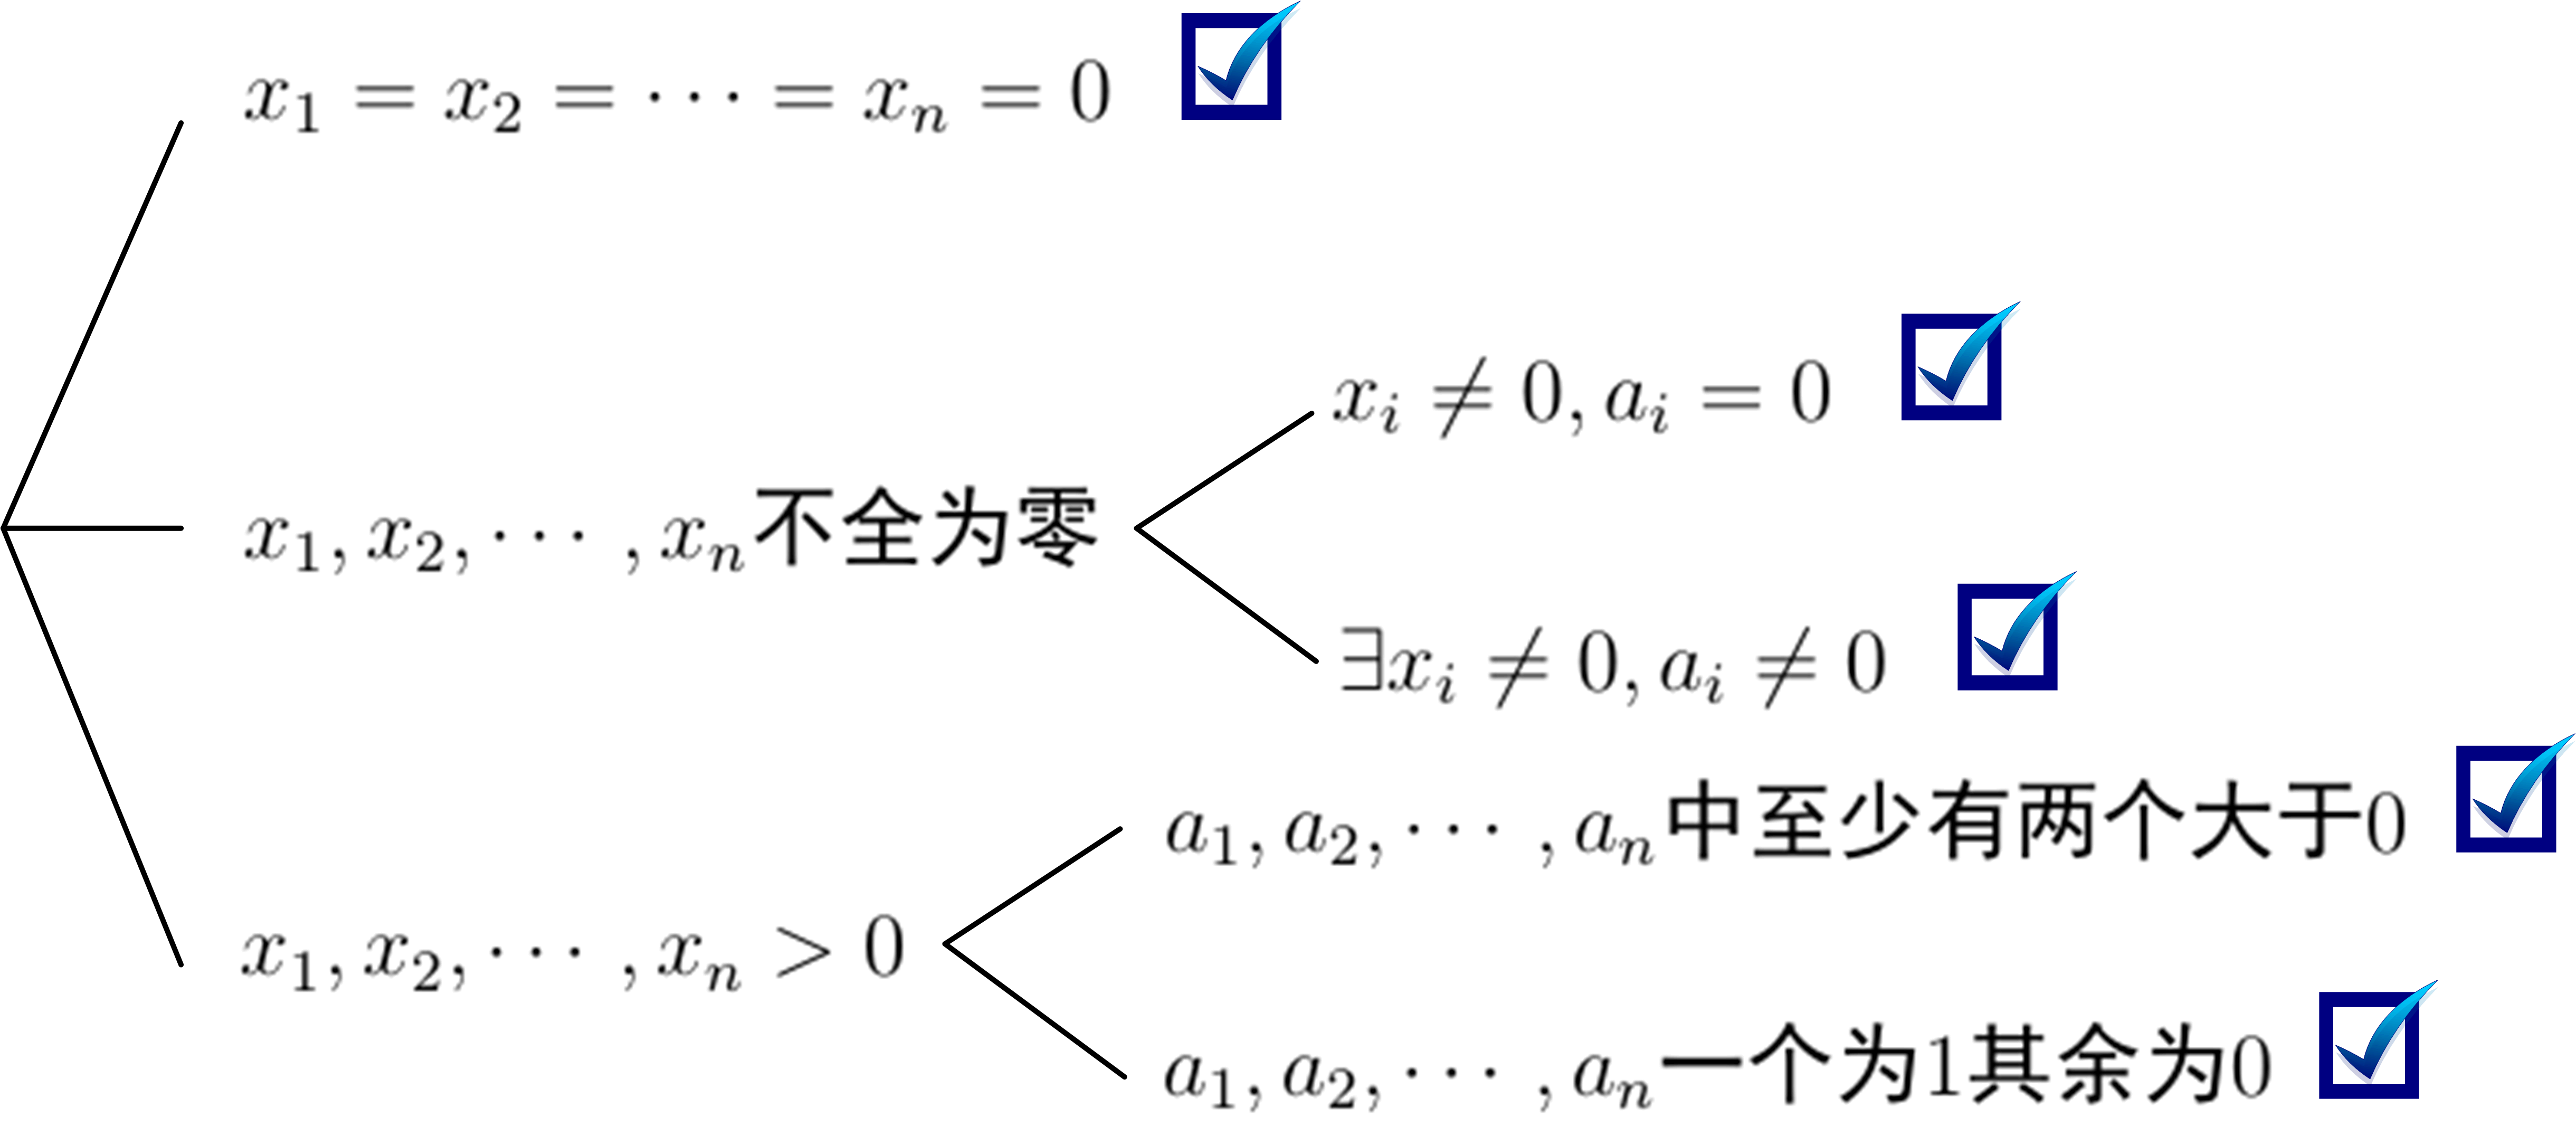
\includegraphics[height=0.2\textheight]{F:/life/2018AutumnTA/Exercises/8/Tree.png}
\end{center}
\end{figure}
对于这种问题,同时考虑$x_i,i=1,2,\cdots,n$和$a_i,i=1,2,\cdots,n$的分类不太容易. 可首先对$x_i,i=1,2,\cdots,n$进行分类,在每个$x_i$类别之下考虑$a_i,i=1,2,\cdots,n$的分类,这样会容易一些. 这也可以视为分而治之(Divide and conquer)思想的一个应用,先找到一个分类,在每一种类别之下剩余的问题可以更简单.
}

\item作下列函数的图形:
\newline
(1)$y=x^3+6x^2-15x-20$;
\newline
(2)$y=\frac{3x}{1+x^2}$;
\newline
(3)$y=\ln\frac{1+x}{1-x}$;
\newline
(4)$y=x+\arctan x$.

解:(1)i)函数的定义域为$(-\infty,+\infty)$

ii)曲线无铅直渐近线,$\lim\limits_{x\rightarrow+\infty}(x^3+6x^2-15x-20)=+\infty,\lim\limits_{x\rightarrow-\infty}(x^3+6x^2-15x-20)=-\infty$故无水平渐近线,$\lim\limits_{x\rightarrow+\infty}\frac yx=\lim\limits_{x\rightarrow+\infty}\frac{x^3+6x^2-15x-20}x=+\infty,\lim\limits_{x\rightarrow+\infty}\frac yx=\lim\limits_{x\rightarrow-\infty}\frac{x^3+6x^2-15x-20}x=-\infty$,故无斜渐近线;

iii)$y'=3x^2+12x-15=3(x^2+4x-5)=3(x+5)(x-1),y''=6x+12$,令$y'=0$得$x=-5$或$x=1$,$y''(-5)=-18<0,y''(1)=18>0$,故$(-5,80)$是函数的极大值点,$(1,-28)$是函数的极小值点,当$x=-2$时$y''=0$,故$(-2,26)$是函数的拐点

iv)当$x<-5$时$y'>0,y''<0$,函数单调增加且上凸,当$-5<x<-2$时$y'<0,y''$,当$x>1$时$y'<0,y''<0$函数单调减少且上凸,当$-2<x<1$时$y'<0,y''>0$函数单调减少且下凸,当$x>1$时$y'>0,y''>0$函数单调增加且上凸,如下表所示:
\begin{table}[H]
\centering
\begin{tabular}{c|c|c|c|c|c|c|c|c|c}
\hline
$x$ & $-\infty$ & $(-\infty,-5)$ & -5 & $(-5,-2)$ & -2 & $(-2,1)$ & 1 & $(1,+\infty)$ & $+\infty$\\
\hline
$y'$ & & + & 0 & - &  & - & 0 & + &\\
\hline
$y''$ & & - & 0 & - &  & + & 0 & + &\\
\hline
$y$ & $-\infty$ & 上凸$\nearrow$ & 极大值80 & 上凸$\searrow$ & 拐点 & 下凸$\searrow$ & 极小值-28 & 下凸$\nearrow$ & $+\infty$\\
\hline
\end{tabular}
\end{table}
可据此画出函数的略图.
\begin{figure}[H]
\begin{center}
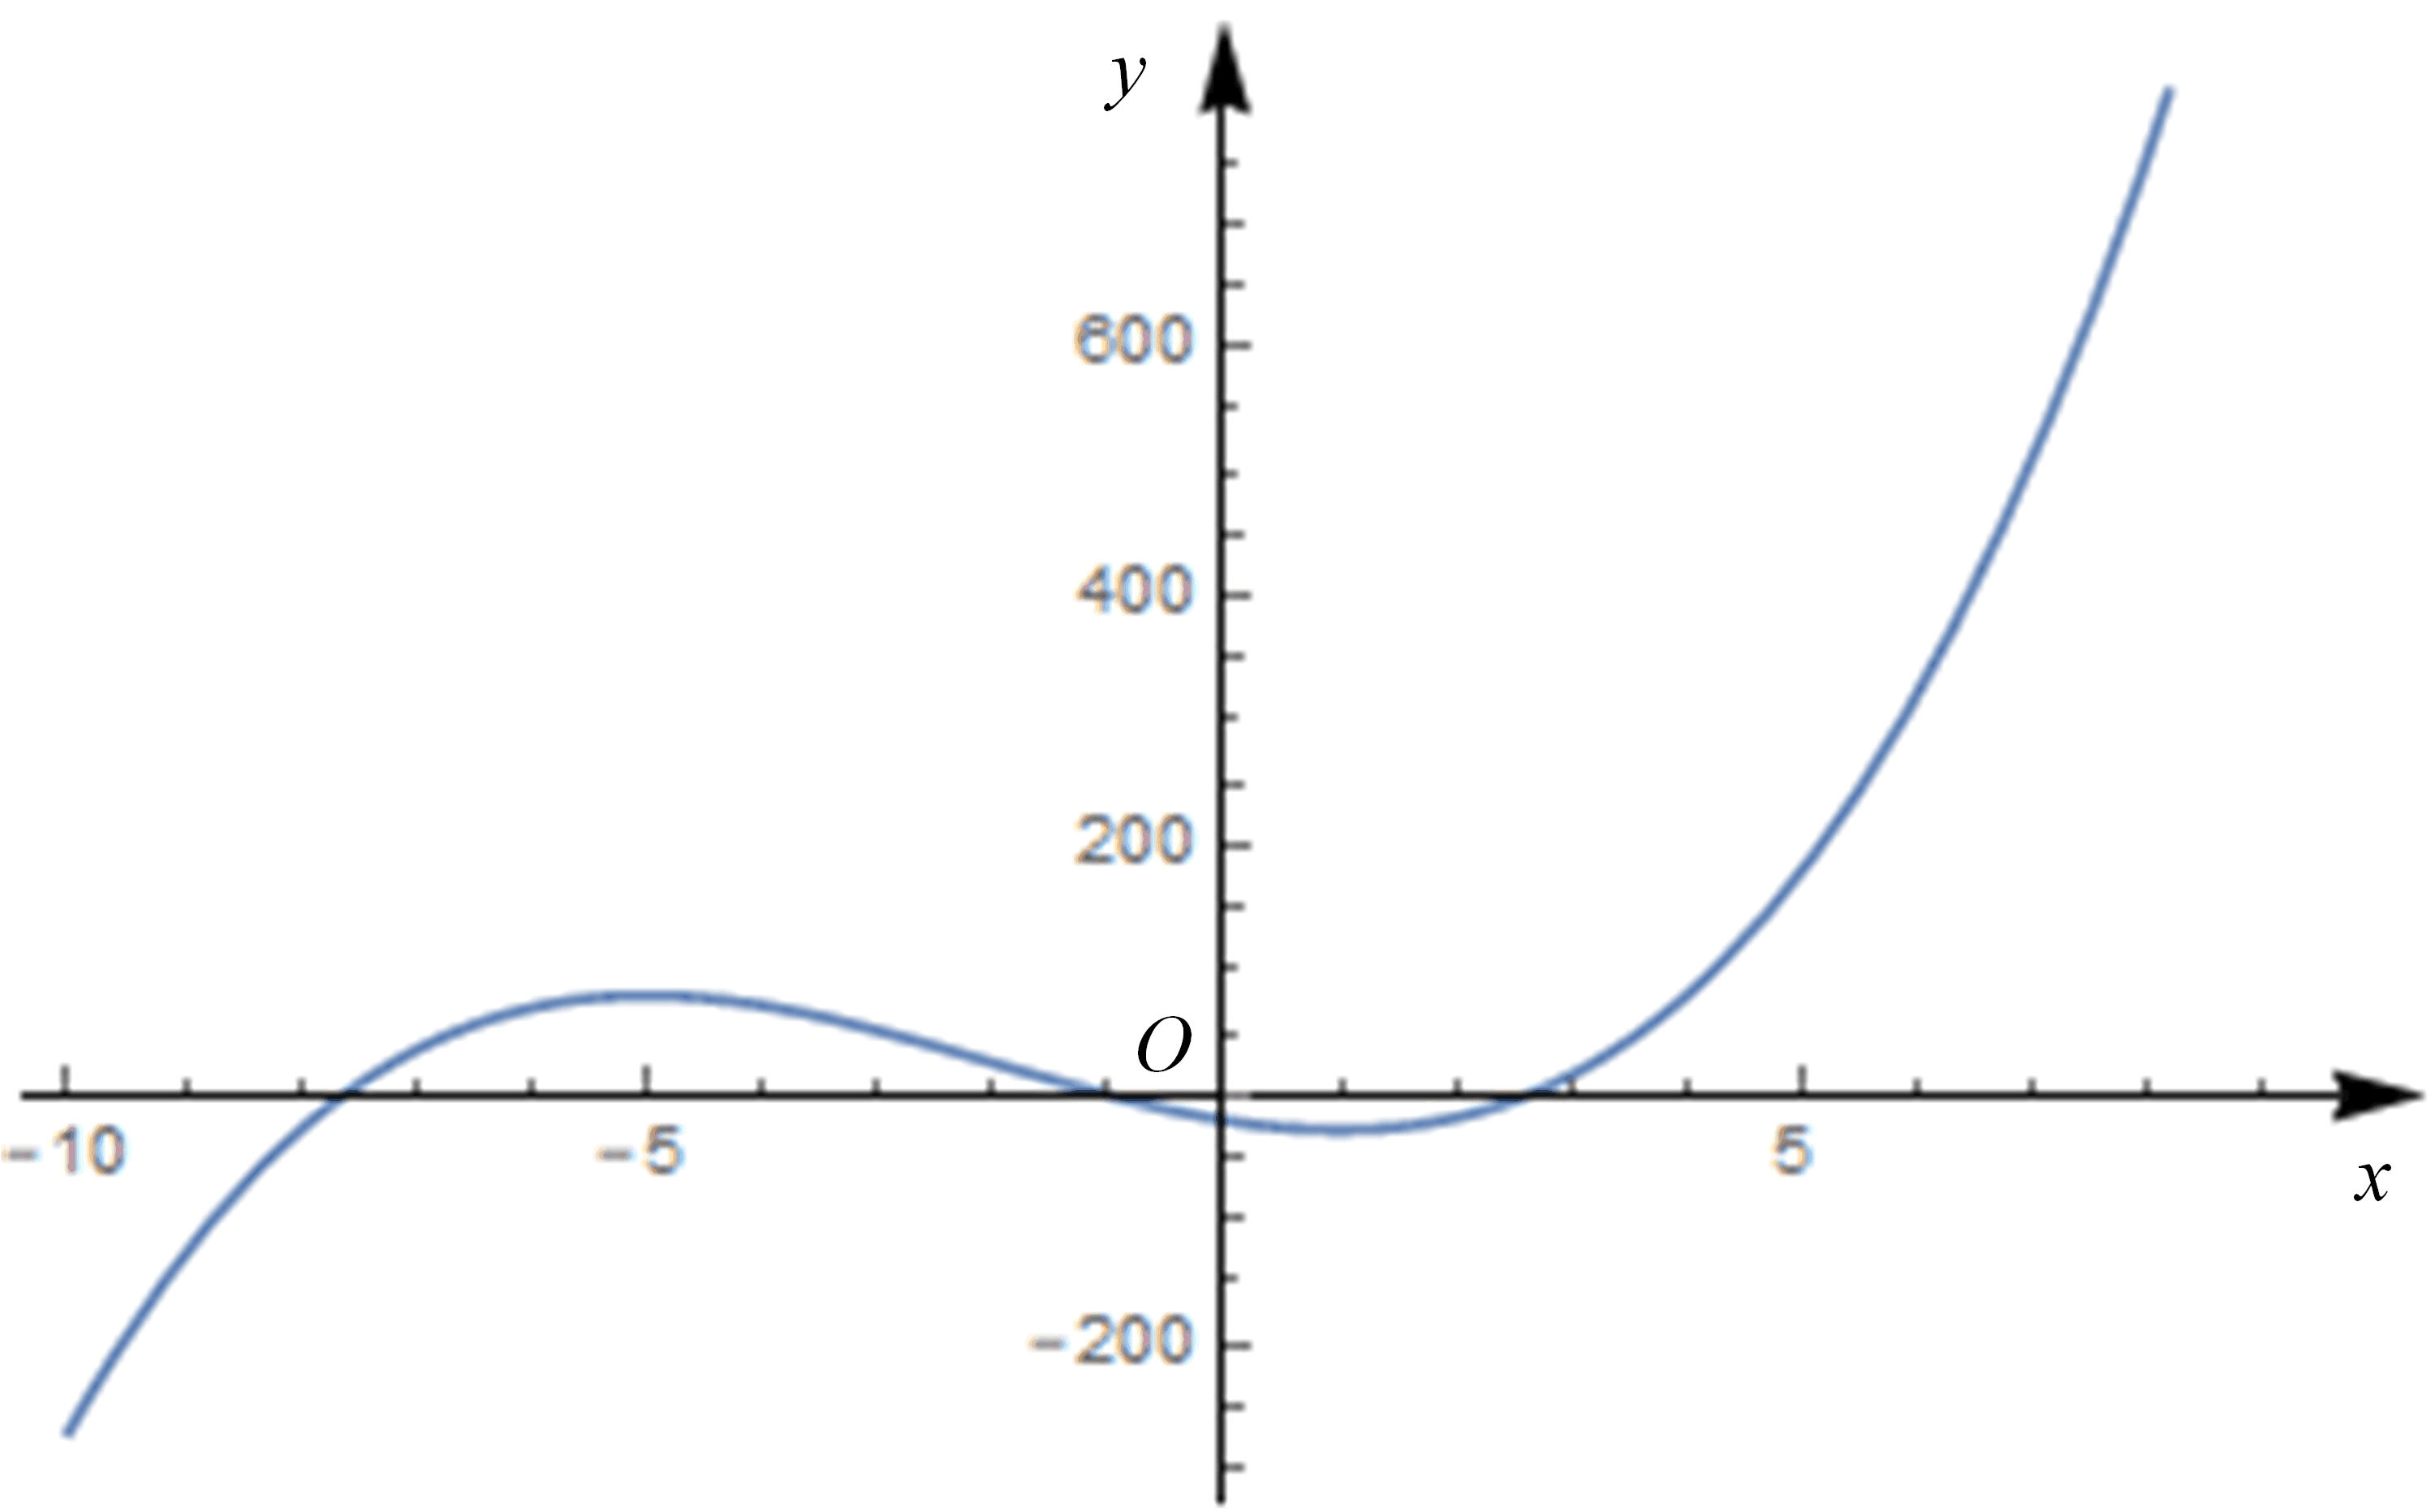
\includegraphics[height=0.2\textheight]{F:/life/2018AutumnTA/Exercises/8/Fig1-1.png}
\end{center}
\end{figure}

(2)i)函数的定义域为$(-\infty,+\infty)$,为奇函数故可仅对$[0,+\infty)$区间进行分析;

ii)$\lim\limits_{x\rightarrow\infty}\frac{3x}{1+x^2}=0$,故水平渐近线为$y=0$,$\lim\limits_{x\rightarrow\infty}\frac yx=\frac{3}{1+x^2}=0,\lim\limits_{x\rightarrow\infty}(\frac{3x}{1+x^2}-0)=0$,故无斜渐近线;

iii)$y'=\frac{3(1+x^2)-3x\cdot2x}{(1+x^2)^2}=\frac{3-3x^2}{(1+x^2)^2}=\frac{3(1-x)(1+x)}{(1+x^2)^2},y''=\frac{-6x(1+x^2)^2-[-3x^2\cdot2(1+x^2)\cdot2x]}{(1+x^2)^4}=\frac{-6x(1-x)(1+x)}{(1+x^2)^3}$. 令$y'=0$得$x=-1$或$x=1$,令$y''=0$得$x=-1$或$x=1$,函数的拐点为$(-1,-\frac32)$和$(1,\frac32)$;

iv)当$x<-1$时$y'<0,y''>0$,函数单调减少且下凸,当$-1<x<1$时$y'>0,y''<0$,函数单调增加且上凸,当$x>1$时$y'<0,y''>0$,函数单调减少且下凸. 故$(-1,-\frac32)$是函数的极小值点,$(1,\frac32)$是函数的极大值点. 如下表所示:
\begin{table}[H]
\centering
\begin{tabular}{c|c|c|c|c|c|c|c}
\hline
$x$ & $-\infty$ & $(-\infty,-1)$ & -1 & $(-1,1)$ & 1 & $(1,+\infty)$ & $+\infty$\\
\hline
$y'$ & & - & 0 & + & 0 & - &\\
\hline
$y''$ & & + & 0 & - & 0 & + & \\
\hline
$y$ & 0 & 下凸$\searrow$ & 极小值$-\frac32$、拐点 & 上凸$\nearrow$ & 极大值$\frac32$、拐点 & 下凸$\searrow$ & 1\\
\hline
\end{tabular}
\end{table}
可据此画出函数的略图.
\begin{figure}[H]
\begin{center}
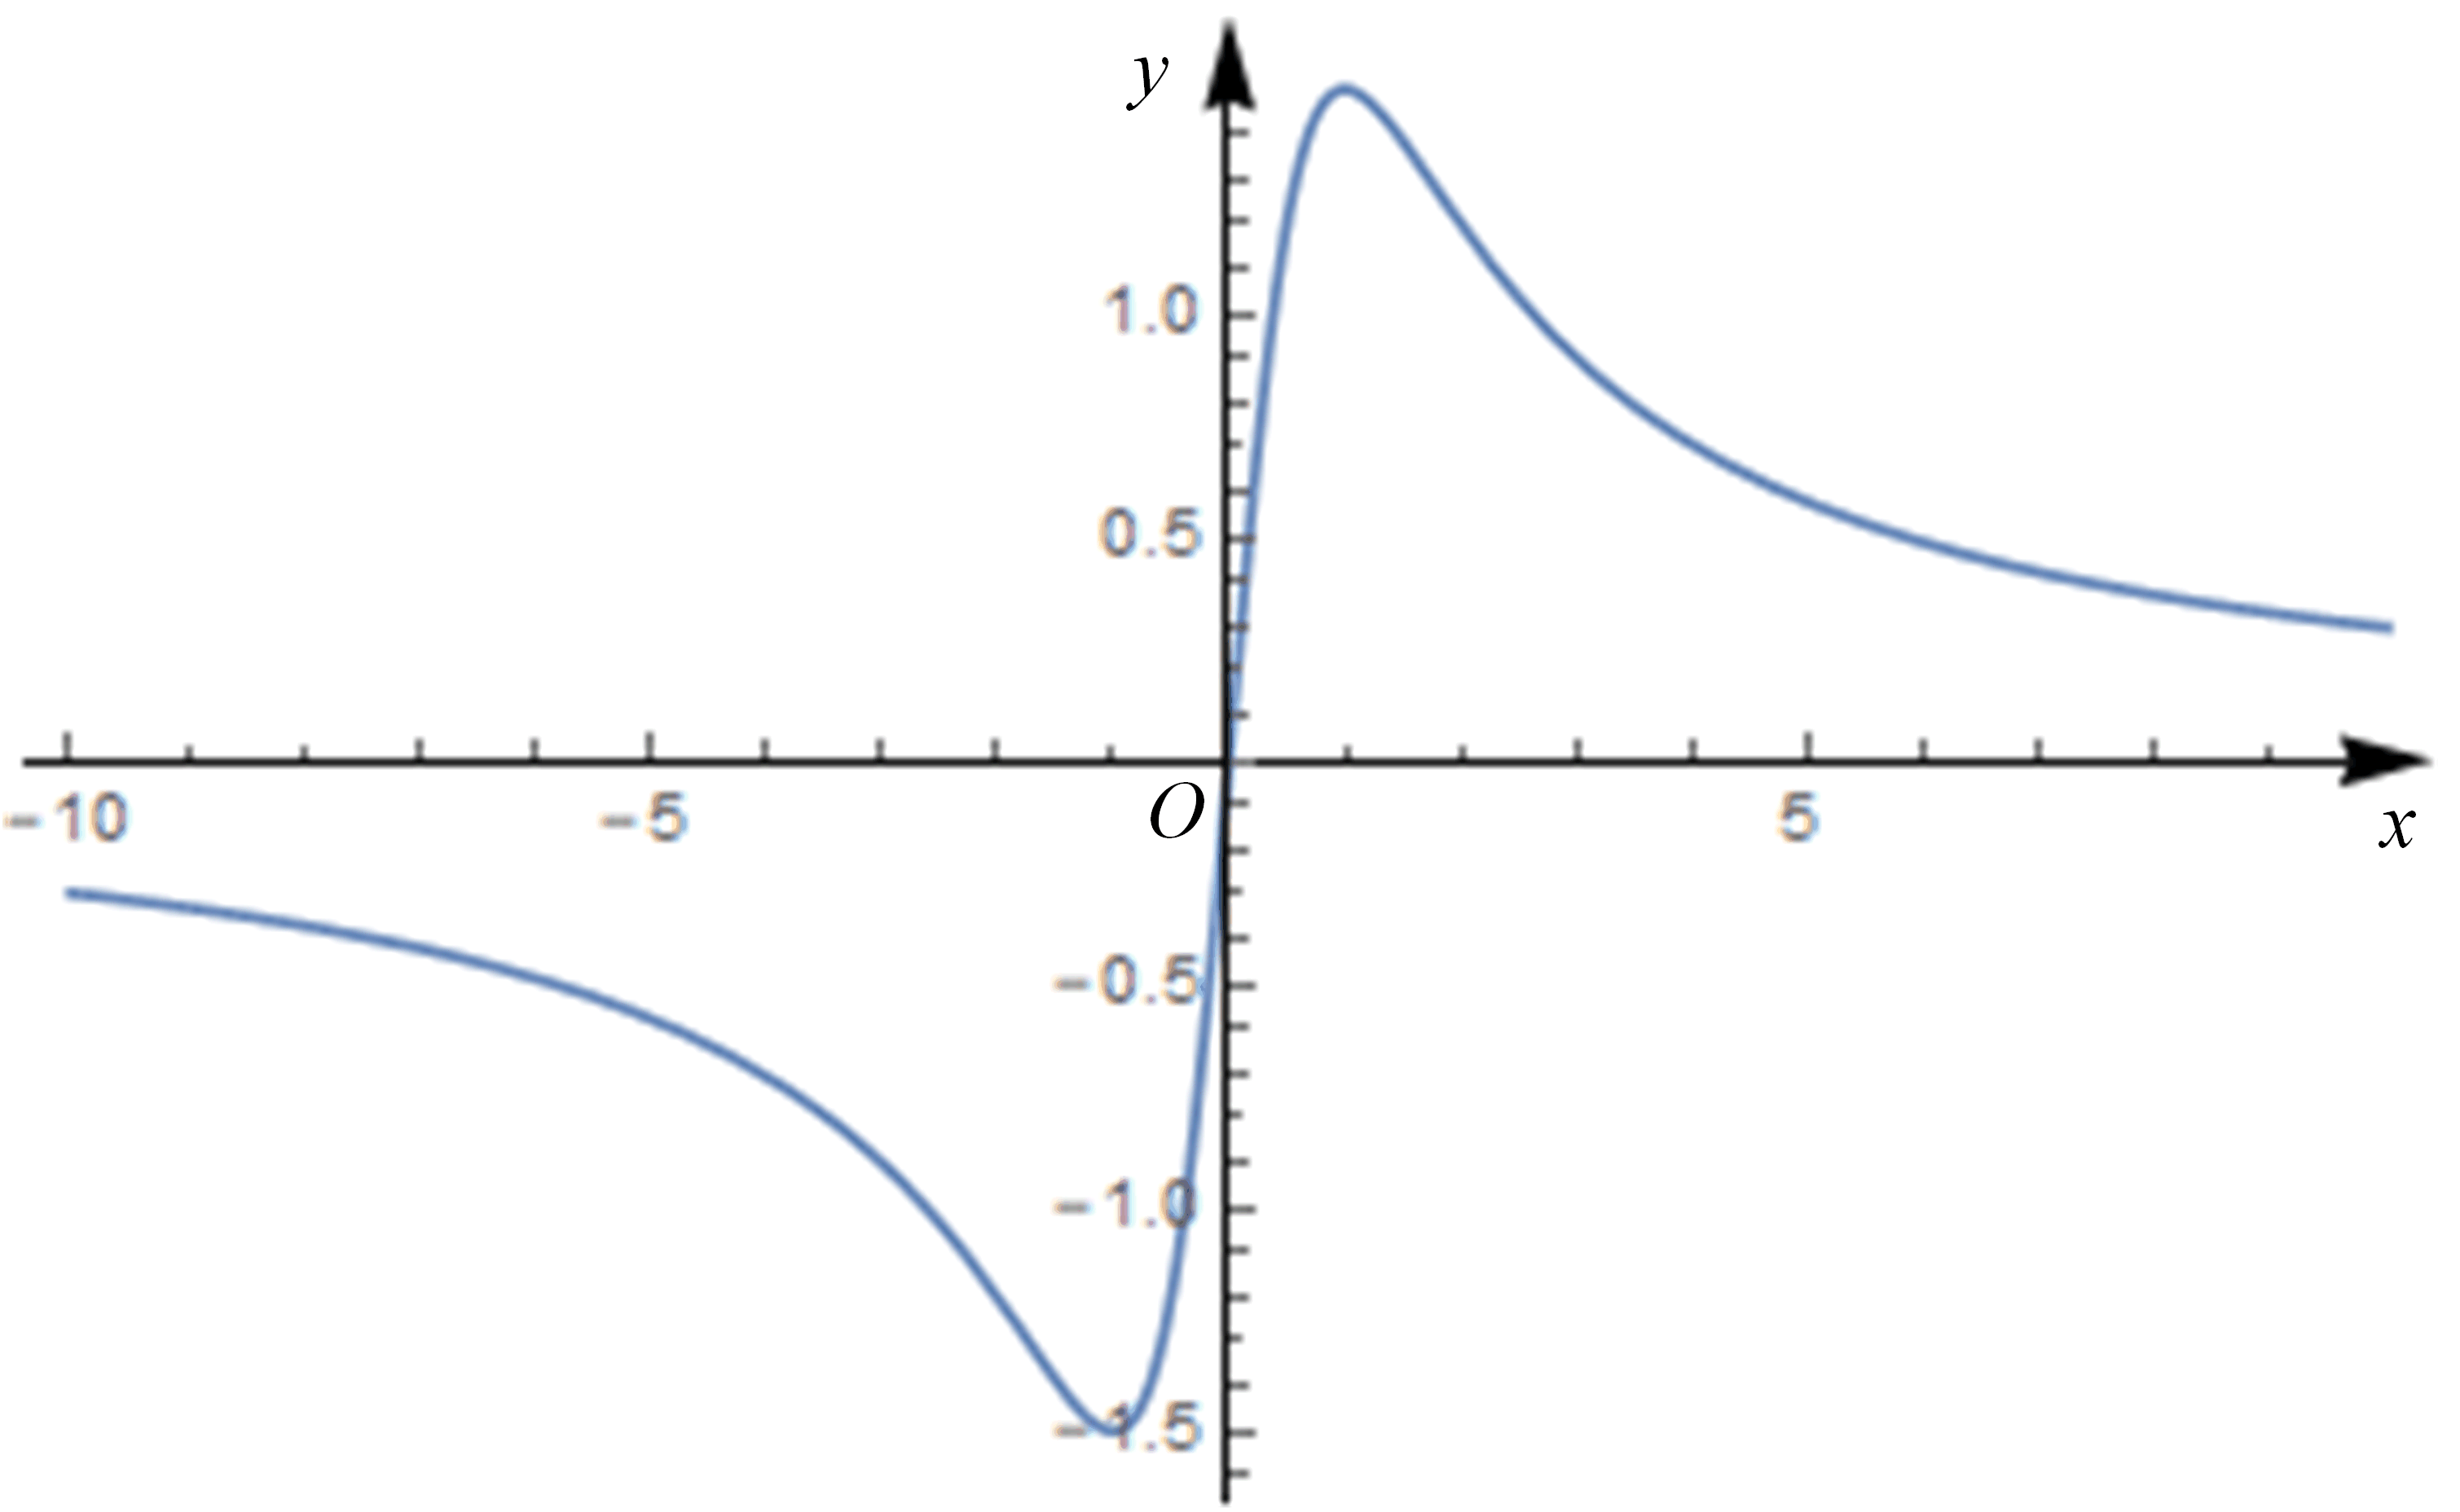
\includegraphics[height=0.2\textheight]{F:/life/2018AutumnTA/Exercises/8/Fig2-1.png}
\end{center}
\end{figure}

(3)i)由$\frac{1+x}{1-x}>0$得函数的定义域为$(-1,1)$,$y(-x)=\ln\frac{1-x}{1+x}=-\ln\frac{1+x}{1-x}=-y(x)$,故函数为奇函数;

ii)$\lim\limits_{x\rightarrow-1^+}\ln\frac{1+x}{1-x}=\lim\limits_{x\rightarrow-1^+}\ln\frac{1+x}{1-x}=-\infty,\lim\limits_{x\rightarrow1^-}\ln\frac{1+x}{1-x}=+\infty$,故函数有两条铅直渐近线$x=-1,x=1$;

iii)$y'=\frac1{1+x}+\frac1{1-x}=\frac2{(1-x)(1+x)}>0,y''=\frac{-1}{(1+x)^2}+\frac1{(1-x)^2}=\frac{4x}{(1-x)^2(1+x)^2}$,当$x=0$时$y''=0$,故函数的拐点为$(0,0)$;

iv)当$-1<x<0$时$y''<0$,函数单调增加且上凸,当$0<x<1$时,函数单调减少且下凸. 如下表所示:
\begin{table}[H]
\centering
\begin{tabular}{c|c|c|c|c|c}
\hline
$x$ & -1 & $(-1,0)$ & 0 & $(0,1)$ & 1 \\
\hline
$y'$ &  & + & 2 & + & \\
\hline
$y''$ &  & - & 0 & + & \\
\hline
$y$ & $-\infty$ & 上凸$\nearrow$ & 拐点 & 下凸$\nearrow$ & +$\infty$\\
\hline
\end{tabular}
\end{table}
可据此画出函数的略图.
\begin{figure}[H]
\begin{center}
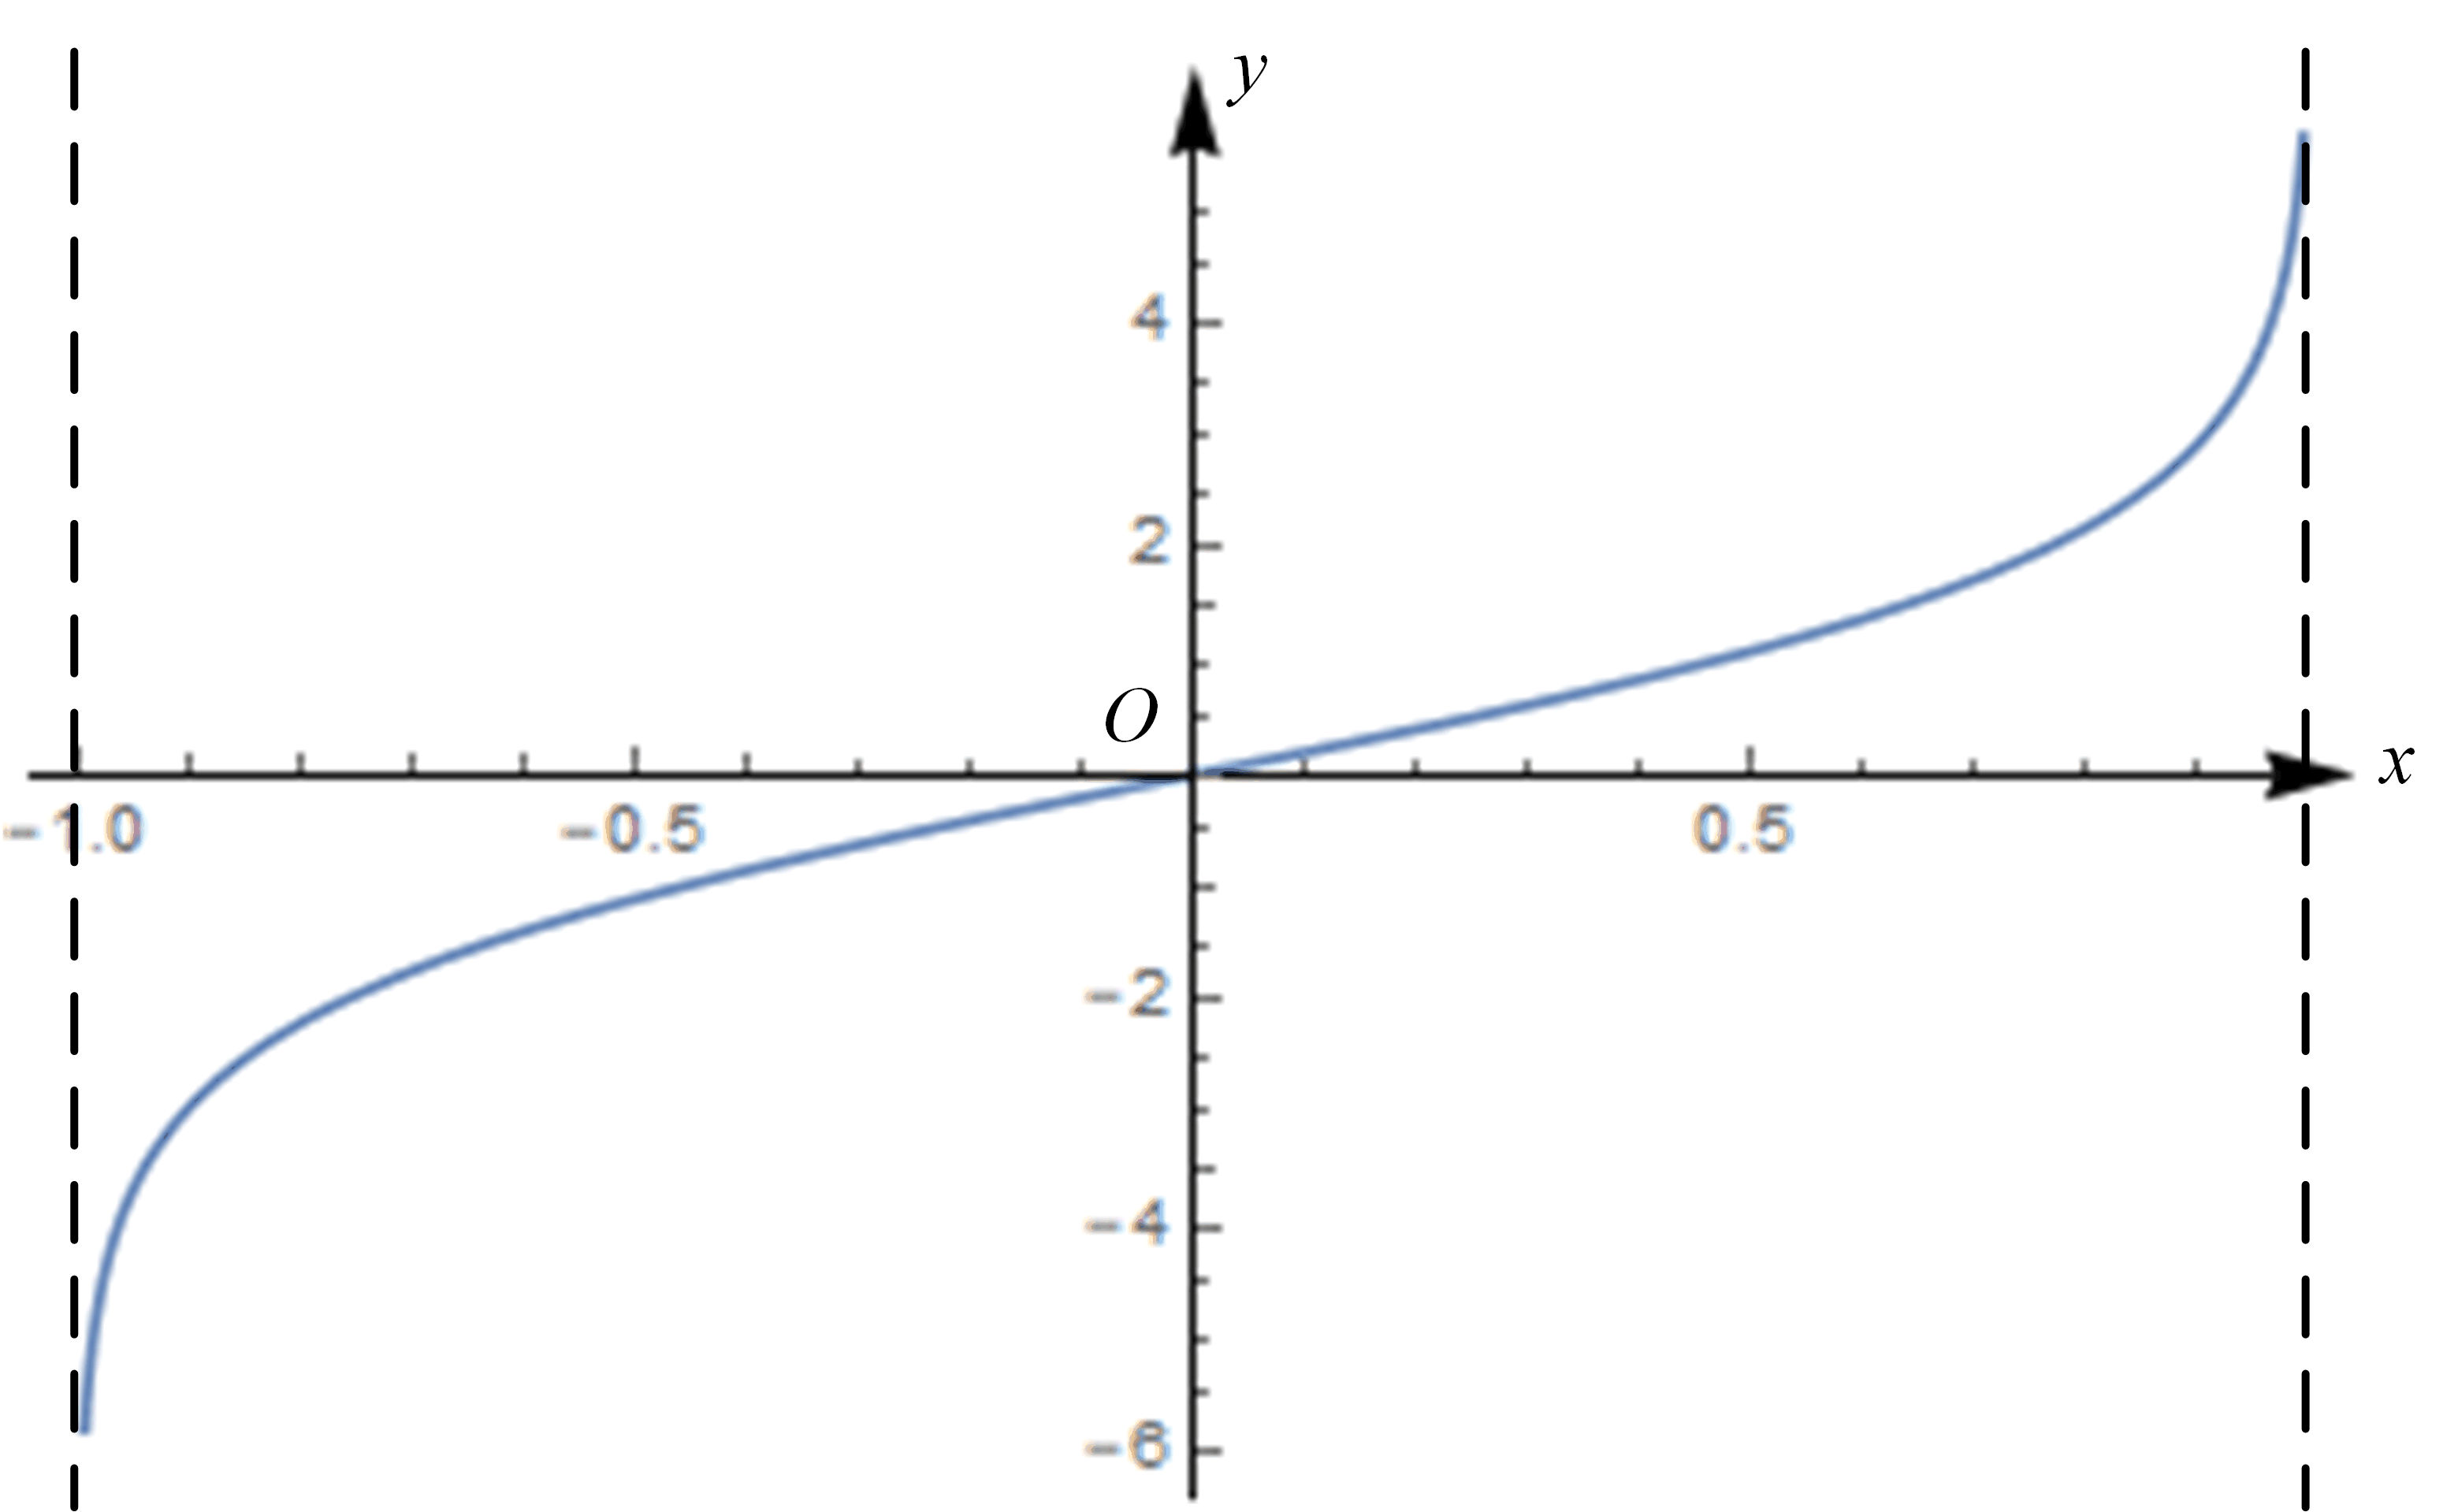
\includegraphics[height=0.2\textheight]{F:/life/2018AutumnTA/Exercises/8/Fig3-1.png}
\end{center}
\end{figure}

(4)i)函数的定义域为$(-\infty,+\infty)$,易知函数为奇函数;

ii)函数无铅直渐近线,$\lim\limits_{x\rightarrow+\infty}(x+\arctan x)=+\infty,\lim\limits_{x\rightarrow-\infty}(x+\arctan x)=-\infty$,故无水平渐近线,$\lim\limits_{x\rightarrow+\infty}\frac yx=\lim\limits_{x\rightarrow+\infty}\frac{x+\arctan x}x=1,\lim\limits_{x\rightarrow+\infty}(y-x)=\lim\limits_{x\rightarrow+\infty}\arctan x=\frac\pi2$,故有斜渐近线$y=x+\frac\pi2$和$y=x-\frac\pi2$;

iii)$y'=1+\frac1{1+x^2}>0,y''=-\frac{2x}{(1+x^2)^2}$,函数有一个拐点$(0,0)$;

iv)当$x<0$时$y''>0$函数单调增加且下凸,当$x>0$时$y''<0$,函数单调增加且下凸. 如下表所示:
\begin{table}[H]
\centering
\begin{tabular}{c|c|c|c|c|c}
\hline
$x$ & $-\infty$ & $(-\infty,0)$ & 0 & $(0,+\infty)$ & $+\infty$\\
\hline
$y'$ & & + &  & + &\\
\hline
$y''$ & & - & 0 & + &\\
\hline
$y$ & $x-\frac\pi2$ & 上凸$\nearrow$ & 拐点 & 下凸$\nearrow$ & $x+\frac\pi2$\\
\hline
\end{tabular}
\end{table}

可据此画出函数的略图.
\begin{figure}[H]
\begin{center}
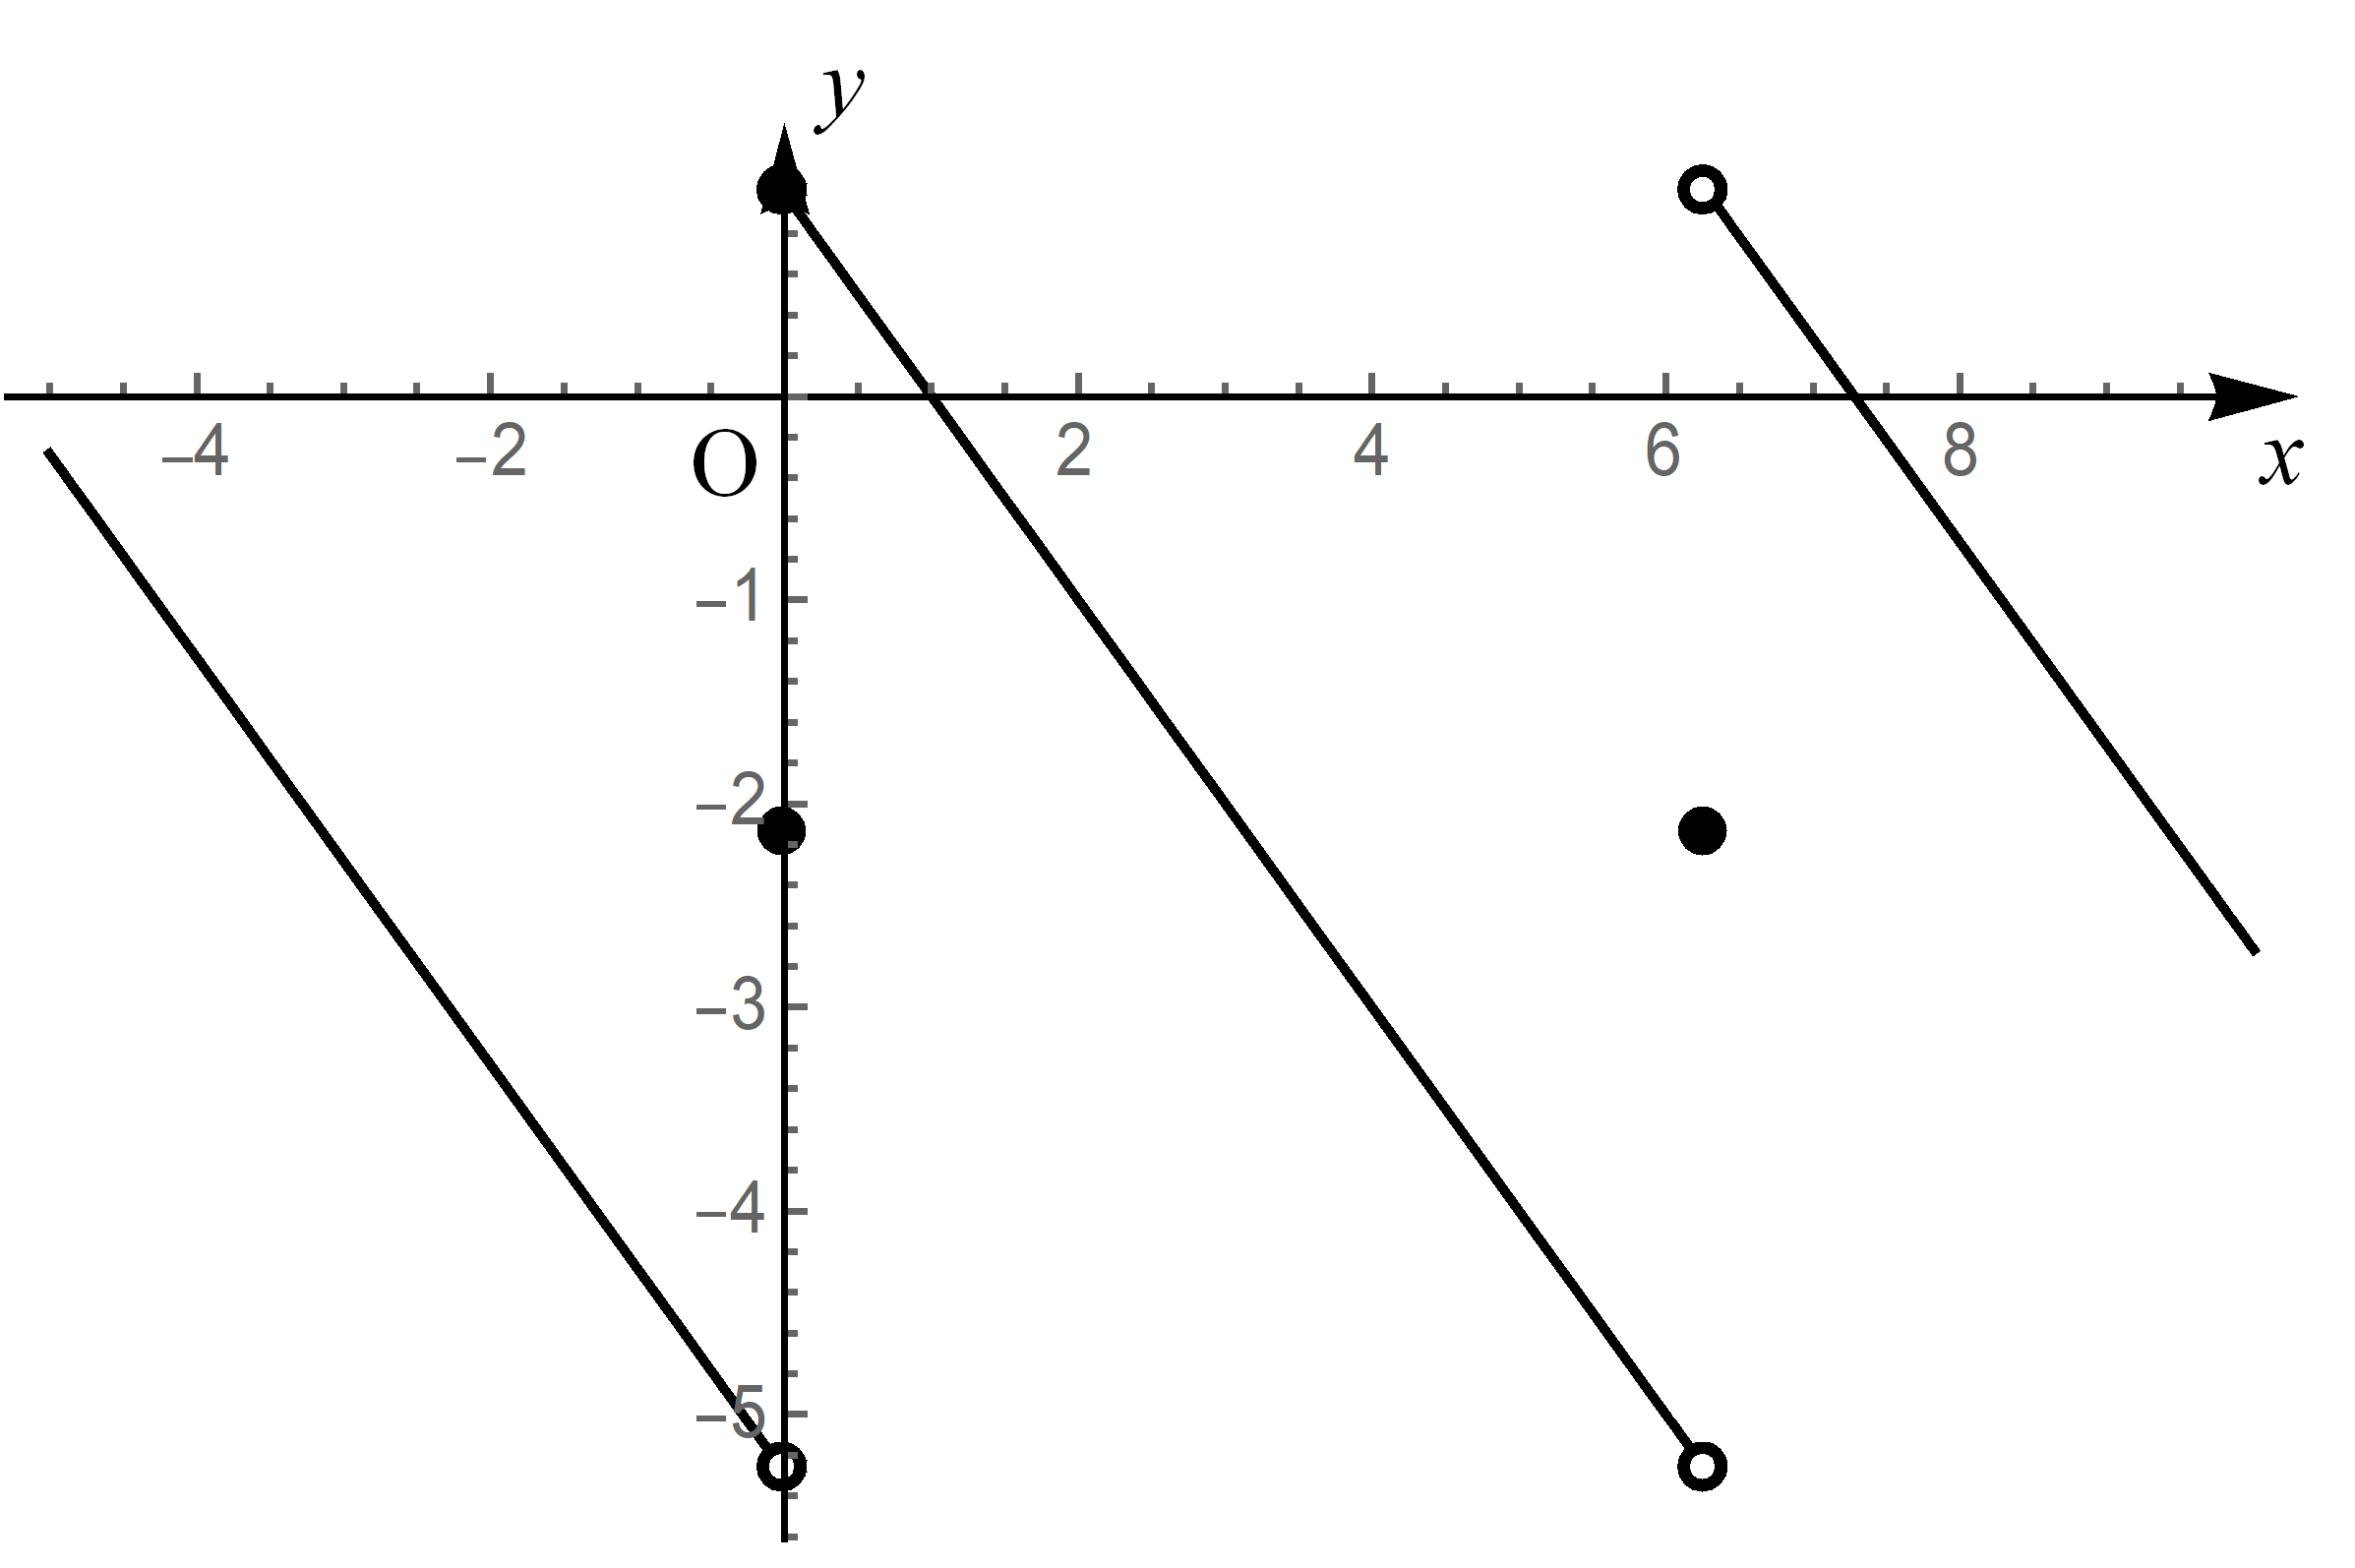
\includegraphics[height=0.2\textheight]{F:/life/2018AutumnTA/Exercises/8/Fig4-1.png}
\end{center}
\end{figure}

\item已知$y=f(x)$是由方程$y^3-x^3+2xy=0$所确定的隐函数,设曲线$y=y(x)$有斜渐近线$y=ax+b$,求$a,b$.

解:$\because$曲线有斜渐近线

$\therefore\lim\limits_{x\rightarrow+\infty}\frac yx=a$存在

将方程$y^3-x^3+2xy=0$两边同除以$x^3$并取极限得$a^3-1-0=0$,故$a=1$

将$y^3-x^3+2xy=(x-y)(x^2+xy+y^2)+2xy=0$两边同除以$x^2$并取极限得$[\lim\limits_{x\rightarrow+\infty}(x-y)](1+a+a^2)+2a=0$,故$b=-\lim\limits_{x\rightarrow+\infty}(x-y)=\frac{-2a}{1+a+a^2}=-\frac23$.
\end{enumerate}
\subsection{习题5.5解答}
\begin{enumerate}
\item按指定次数写出下列函数在指定点的泰勒多项式:
\newline
(1)$f(x)=\frac{1+x+x^2}{1-x+x^2},x_0=0$,展到4次;
\newline
(2)$f(x)=\ln\cos x,x_0=0$,展到6次;
\newline
(3)$f(x)=\sqrt x,x_0=1$,展到4次;
\newline
(4)$f(x)=1+2x-4x^2+x^3+6x^4,x_0=1$,展到6次;
\newline
(5)$f(x)=\frac x{x-1},x_0=2$,展到$n$次;
\newline
(6)$f(x)=x^3\ln x,x_0=1$,展到5次.

解:(1)方法1:$f(x)(1-x+x^2)=1+x+x^2,f(0)=1$

$f'(x)(1-x+x^2)+f(x)(-1+2x)=1+2x,f'(0)=2$

$f''(x)(1-x+x^2)+2f'(x)(-1+2x)+f(x)2=2,f''(0)=4$

$f'''(x)(1-x+x^2)+3f''(x)(-1+2x)+3f'(x)2=0,f'''(0)=0$

$f^{(4)}(x)(1-x+x^2)+4f'''(x)(-1+2x)+6f''(x)2=0,f''''(0)=-48$

$\therefore f(x)=f(0)+f'(0)x+\frac{f''(0)}{2!}x^2+\frac{f'''(0)}{3!}x^3+\frac{f''''(0)}{4!}x^4+o(x^4)=1+2x+2x^2-2x^4+o(x^4)$.

方法2:
\[\begin{split}
f(x)&=\frac{1+x+x^2}{1-x+x^2}=\frac{(1+x+x^2)(x-1)}{(1-x+x^2)(x+1)}\frac{x+1}{x-1}\\
&=\frac{x^3-1}{x^3+1}\frac{x+1}{x-1}=(1-\frac2{1+x^3})(1-\frac2{1-x})\\
&=\{1-2[\sum_{k=0}^n(-x^3)^k+o(x^{3n})]\}\{1-2[\sum_{k=0}^nx^k+o(x^n)]\}\\
&=\{1-2[1-x^3+o(x^4)]\}\{1-2[1+x+x^2+x^3+x^4+o(x^4)]\}\\
&=[-1+2x^3+o(x^4)][-1-2x-2x^2-2x^3-2x^4+o(x^4)]\\
&=1+2x+2x^2+(2-2)x^3+(2-4)x^4+o(x^4)\\
&=1+2x+2x^2-2x^4+o(x^4).
\end{split}\]
(2)方法1:$f(x)=\ln\cos x,f(0)=0$

$f'(x)=\frac{-\sin x}{\cos x}=-\tan x,f'(0)=0$

$f''(x)=-\sec^2x,f''(0)=-1$

$f'''(x)=-2\sec x\sec x\tan x=2\sec^2x\tan x,f'(0)=0$

$f^{(4)}(x)=-4\sec x\sec x\tan x\tan x-2\sec^2x\sec^2x=-2\sec^2x(2\tan^2x+\sec^2x),f''''(0)=-2$

$f^{(5)}(x)=-4\sec x\sec x\tan x(2\tan^2x+\sec^2x)-2\sec^2x(4\tan x\sec^2x+2\sec x\sec x\tan x)=-4\sec^2x\tan x(2\tan^2x+\sec^2x)-2\sec^2x(6\tan x\sec^2x)=-8\sec^2x\tan^3x-16\sec^4x\tan x=-8\sec^2x\tan x(\tan^2x+2\sec^2x),f^{(5)}(0)=0$

$f^{(6)}=-(16\sec x\tan x+8\sec^4x)(\tan^2x+2\sec^2x)-8\sec^2x\tan x(2\tan x\sec^2x+4\sec x\sec x\tan x),f^{(6)}(0)=-16$

$\therefore f(x)=-\frac12x^2-\frac1{12}x^4-\frac1{45}x^6+o(x^6)$.

方法2:\[\begin{split}
f(x)&=\ln\cos x=\ln[1+(\cos x-1)]\\
&=\sum_{k=1}^n\frac{(-1)^{k-1}}k(\cos x-1)^k+o((\cos x-1)^n)\\
&=\sum_{k=1}^n\frac{(-1)^{k-1}}k[\sum_{i=0}^m\frac{(-1)^{2i}}{(2i)!}x^{2i}+o(x^{2m+1})-1]^k+o(x^{2mn})\\
&=\sum_{k=1}^3\frac{(-1)^{k-1}}k[-\frac1{2!}x^2+\frac1{4!}x^4-\frac1{6!}x^6+o(x^6)]^k+o(x^{18})\\
&=-\frac1{2!}x^2+\frac1{4!}x^4-\frac1{6!}x^6+o(x^6)-\frac12[\frac14x^4-2\cdot\frac1{2!\cdot4!}x^6+o(x^6)]+\frac13[-\frac18x^6+o(x^6)]+o(x^{18})\\
&=-\frac12x^2+(\frac1{24}-\frac18)x^4+(-\frac1{720}+\frac1{48}-\frac1{24})x^6+o(x^6)\\
&=-\frac12x^2-\frac1{12}x^4-\frac1{45}x^6+o(x^6).
\end{split}\]
(3)方法1:$f(x)=\sqrt x,f(1)=1$

$f'(x)=\frac1{2\sqrt x},f'(1)=\frac12$

$f''(x)=\frac{-1}{4x^{\frac32}},f''(1)=-\frac14$

$f'''(x)=\frac{3}{8x^{\frac52}},f'''(1)=\frac38$

$f^{(4)}=\frac{-15}{16x^{\frac72}},f^{(4)}=-\frac{15}{16}$

$\therefore f(x)=f(1)+f'(1)(x-1)+\frac{f''(1)}{2!}(x-1)^2+\frac{f'''(1)}{3!}(x-1)^3+\frac{f^{(4)}(1)}{4!}(x-1)^4+o(x^4)=1+\frac12(x-1)-\frac18(x-1)^2+\frac1{16}-\frac5{128}(x-1)^4+o((x-1)^4)$.

方法2:\[\begin{split}
f(x)&=\sqrt x=\sqrt{1+(x-1)}\\
&=1+\sum_{k=1}^n\frac{\frac12(-\frac12)(-\frac32)\cdots(\frac12-k+1)}{k!}(x-1)^k+o((x-1)^n)\\
&=1+\frac12(x-1)+\frac{\frac12(-\frac12)}2(x-1)^2+\frac{\frac12(-\frac12)(-\frac32)}6(x-1)^3+\frac{\frac12(-\frac12)(-\frac32)(-\frac52)}{24}(x-1)^4\\
&\hspace{1cm}+o((x-1)^4)\\
&=1+\frac12(x-1)-\frac18(x-1)^2+\frac1{16}(x-1)^3-\frac5{128}(x-1)^4+o((x-1)^4)
\end{split}\]
(4)$f(x)=1+2x-4x^2+x^3+6x^4,f(1)=1+2-4+1+6=6$

$f'(x)=2-8x+3x^2+24x^3,f'(1)=2-8+3+24=21$

$f''(x)=-8+6x+72x^2,f''(1)=-8+6+72=70$

$f'''(x)=6+144x,f'''(1)=150$

$f^{(4)}(x)=144$

$f^{(5)}(x)=0$

$f^{(6)}(x)=0$

$f(x)=6+21(x-1)+35(x-1)^2+25(x-1)^3+6(x-1)^4+o((x-1)^6)$.

(5)$f(x)=\frac x{x-1},f(2)=2$

$f'(x)=\frac{(x-1)-x}{(x-1)^2}=\frac{-1}{(x-1)^2},f'(2)=-1$

$f''(x)=\frac{2}{(x-1)^3},f''(2)=2$

$f^{(n)}(x)=\frac{(-1)^nn!}{(x-1)^{n+1}}$

$f(x)=f(2)+\sum_{k=1}^n\frac{f^{(k)}}{k!}(x-1)^{k}=2+\sum_{k=1}^n\frac{(-1)^kk!}{k!}(x-1)^{k}=2+\sum_{k=1}^n(-1)^k(x-1)^{k}$.

方法2:\[\begin{split}
f(x)&=\frac x{x-1}=\frac{x-1+1}{x-1}=1+\frac1{x-1}=1+\frac1{1+(x-2)}\\
&=1+\sum_{k=0}^n[-(x-2)]^k+o((x-2)^n)\\
&=2+\sum_{k=1}^n[-(x-2)]^k+o((x-2)^n)
\end{split}\]
(6)方法1:$f(x)=x^3\ln x,f(1)=0$

$f'(x)=3x^2\ln x+x^3\frac1x=x^2(3\ln x+1),f'(1)=1$

$f''(x)=2x(3\ln x+1)+x^2\frac3x=x(6\ln x+5),f''(1)=5$

$f'''(x)=6\ln x+5+x\frac6x=6\ln x+11,f'''(1)=11$

$f^{(4)}(x)=\frac6x,f^{(4)}(1)=6$

$f^{(5)}(x)=-\frac6{x^2},f^{(5)}(1)=-6$

$f(x)=f(1)+f'(1)(x-1)+\frac{f''(1)}{2!}(x-1)^2+\frac{f'''(1)}{3!}(x-1)^3+\frac{f^{(4)}(1)}{4!}(x-1)^4+\frac{f^{(5)}(1)}{5!}(x-1)^5+o((x-1)^5)=(x-1)+\frac52(x-1)^2+\frac{11}6(x-1)^3+\frac14(x-1)^4-\frac1{20}(x-1)^5+o((x-1)^5)$.

方法2:\[\begin{split}
f(x)&=x^3\ln x=[1+(x-1)]^3\ln[1+(x-1)]\\
&=[1+3(x-1)+\frac{3\cdot2}{2!}(x-1)^2+\frac{3\cdot2\cdot1}{3!}(x-1)^3][\sum_{k=1}^n\frac{(-1)^{k-1}}k(x-1)^k+o((x-1)^n)]\\
&=[1+3(x-1)+3(x-1)^2+(x-1)^3][(x-1)-\frac12(x-1)^2+\frac13(x-1)^3-\frac14(x-1)^4\\
&\hspace{1cm}+\frac15(x-1)^5+o((x-1)^5)]\\
&=(x-1)+(3-\frac12)(x-1)^2+(\frac13-\frac32+3)(x-1)^3+(1-\frac32+1-\frac14)(x-1)^4\\
&\hspace{1cm}+(-\frac12+1-\frac34+\frac15)(x-1)^5+o((x-1)^5)\\
&=(x-1)+\frac52(x-1)^2+\frac{11}6(x-1)^3+\frac14(x-1)^4-\frac1{20}(x-1)^5+o((x-1)^5).
\end{split}\]
\item设函数$f(x)$在点$x_0$附近有$n+1$阶连续导数且$f'(x_0)=\cdots=f^{(n)}(x_0)=0,f^{(n+1)}(x_0)\neq0$,证明:若$n$为奇数,则点$x_0$是$f(x)$的极值点;若$n$为偶数,则点$x_0$不是$f(x)$的极值点.

证明:{\bf方法1:}$\because f(x)$在点$x_0$附近有$n+1$阶连续导数且$f'(x_0)=\cdots=f^{(n)}(x_0)=0,f^{(n+1)}(x_0)\neq0$

$\therefore$在$x_0$的某个去心邻域$N^*(x_0)$内$f^{(n+1)}(x)\neq0$且在该邻域内$f(x)=f(x_0)+\frac{f^{(n+1)}(\xi)}{(n+1)!}(x-x_0)^{n+1}$,$\xi$介于$x$和$x_0$之间

{\bf正确做法:}当$n$为奇数时,在$N^*(x_0)$内$f(x)-f(x_0)=\frac{f^{(n+1)}(\xi)}{(n+1)!}(x-x_0)^{n+1}$与$f^{(n+1)}(\xi)$同号,故$x_0$是$f(x)$的极值点;当$n$为偶数时,在$N^*(x_0)$内$f(x)-f(x_0)=\frac{f^{(n+1)}(\xi)}{(n+1)!}(x-x_0)^{n+1}$在$x_0$两侧异号,故$x_0$不是$f(x)$的极值点. 

{\bf可能有问题的做法:}{\bf\color{red}{$\therefore f'(x)=\frac{f^{(n+1)}(\xi)}{n!}(x-x_0)^n$}

当$n$为偶数时$f'(x)$在$x_0$两侧附近同号,故点$x_0$不是$f(x)$的极值点;当$n$为奇数时$f'(x)$在$x_0$两侧附近异号,故点$x_0$是$f(x)$的极值点.}

{\bf\color{red}这样做可能有问题,因为$f^{(n+1)}(\xi)$与$x$有关,求导后不一定等于0,即$f'(x)=\frac{f^{(n+1)}(\xi)}{n!}(x-x_0)^n+(\frac{f^{(n+1)}(\xi)}{(n+1)!})'(x-x_0)^{n+1}$}

{\bf方法2:}由$f(x)=\sum_{k=0}^n\frac{f^{(k)}(x_0)}{k!}(x-x_0)^k+o((x-x_0)^n)$及$f'(x_0)=\cdots=f^{(n)}(x_0)=0,f^{(n+1)}(x_0)\neq0$可知
\[
f(x)-f(x_0)=\frac{f^{(n+1)}(x_0)}{(n+1)!}(x-x_0)^{n+1}+o((x-x_0)^{n+1}),
\]
则\[
\lim\limits_{x\rightarrow x_0}\frac{f(x)-f(x_0)}{(x-x_0)^{n+1}}=\frac{f^{(n+1)}(x_0)}{(n+1)!}\neq0
\]
由极限的保号性知存在$x_0$的去心邻域$N^*(x_0)$,在该邻域内$\frac{f(x)-f(x_0)}{(x-x_0)^{n+1}}$与$\frac{f^{(n+1)}(x_0)}{(n+1)!}$同号. 当$n$是奇数时,$f(x)-f(x_0)$与$\frac{f^{(n+1)}(x_0)}{(n+1)!}$非零同号,故$x_0$是$f(x)$的极值点;当$n$是偶数时,$f(x)-f(x_0)$在$x_0$两侧异号,故$x_0$不是$f(x)$的极值点.

{\bf注意:方法2可去掉导数连续这个条件,只需要函数在$x_0$点处有$n+1$阶连续导数,不需要$n+1$阶导数在$x_0$附近连续,方法1则利用了$n+1$阶导数在$x_0$附近连续这个条件.}

\item用泰勒公式进行计算:
\newline
(1)$\sqrt[12]{4000}$,精确到$10^{-4}$;
\newline
(2)$\ln1.02$,精确到$10^{-5}$.

解:(1)令$f(x)=\sqrt[12]{4096-96}=\sqrt[12]{2^{12}-96}=2(1-\frac{96}{4096})^{\frac1{12}}$,$f(x)$在$x=0$处的泰勒多项式的拉格朗日余项为
\[R_n(x)=2\frac{f^{(n+1)}(\xi)}{(n+1)!}x^{n+1}=2\frac{\frac1{12}\cdot(\frac1{12}-1)\cdot\cdots\cdot(\frac1{12}-n)}{(n+1)!}(1+\xi)^{\frac1{12}-n-1}x^{n+1}\]

$\xi$介于$0$和$x$之间. 当$n=1$时
\[\begin{aligned}
|R_1(-\frac{96}{4096})|&=2|\frac{\frac1{12}\cdot(\frac1{12}-1)}{2!}(1+\xi)^{\frac1{12}-2}(-\frac{96}{4096})^2|\\
&=2|\frac{\frac1{12}\cdot(\frac1{12}-1)}{2!}\frac1{(1+\xi)^{2-\frac1{12}}}(-\frac{96}{4096})^2|\\
&<2|\frac{\frac1{12}\cdot(\frac1{12}-1)}{2!}\frac1{(1-\frac{96}{4096})^{2-\frac1{12}}}(-\frac{96}{4096})^2|\\
&<2|\frac{\frac1{12}\cdot(\frac1{12}-1)}{2!}\frac1{(1-\frac{96}{4096})^2}(-\frac{96}{4096})^2|\approx0.000044<10^{-4}
\end{aligned}\]
故$\sqrt[12]{4000}\approx2\sum_{k=0}^1\frac{f^{(k)}(0)}{k!}(-\frac{96}{4096})^k=2+2\frac{1/12}{1!}(-\frac{96}{4096})^1\approx1.9961$.

(2)令$f(x)=\ln(1+x)$,$f(x)$在$x=0$处的泰勒多项式的拉格朗日余项为\\$R_n(x)=\frac{(-1)^n\frac1{(1+\xi)^{n+1}}}{n+1}x^{n+1}$,$\xi$介于$0$和$x$之间. 当$n=2$时
\[
|R_n(0.02)|=|\frac{(-1)^n\frac1{(1+\xi)^{n+1}}}{n+1}0.02^{n+1}|\leq|\frac1{n+1}0.02^{n+1}|\approx2.67\times10^{-6}\leq10^{-5}
\]
故$\ln1.02\approx\sum_{k=1}^2\frac{(-1)^{k-1}}kx^k\approx0.0198$.
\end{enumerate}
%\subsection{第5章补充题}
%\begin{enumerate}
%\item
%\end{enumerate}
\end{document}
\documentclass[12pt,UTF8]{ctexart}
\usepackage{ctex,amsmath,amssymb,geometry,fancyhdr,bm,amsfonts
,mathtools,extarrows,graphicx,url,enumerate,color,float,multicol} 
% 加入中文支持
\newcommand\Set[2]{%
\left\{#1\ \middle\vert\ #2 \right\}}
\geometry{a4paper,scale=0.80}
\pagestyle{fancy}
\rhead{第5章补充题}
\lhead{基础习题课讲义}
\chead{微积分B(1)}
\begin{document}
\def\thesection{8C}
\section{第5章补充题}
\def\thesubsection{\thesection.\arabic{subsection}}
\subsection{第5章补充题解答}
\begin{enumerate}
\item求证$n$次拉盖尔多项式
\[
\mathrm L_n(x)=\mathrm e^x\frac{\mathrm d^n}{\mathrm dx^n}(x^n\mathrm e^{-x})
\]在$(0,+\infty)$上有$n$个相异实根.

证明:首先证明:若$f\in C[a,+\infty),f(a)=0,\lim\limits_{x\rightarrow+\infty}f(x)=0$,且$f(x)$不恒等于$0$,则$\exists\eta\in[a,+\infty),s.t.f'(\eta)=0$.

若存在一点$x_0\in[a,+\infty),s.t.f(x_0)>0$,由于$\lim\limits_{x\rightarrow+\infty}f(x)=0$,所以$\exists X>\mathrm{max}\{a,x_0\},\\
s.t.f(x)<f(x_0)$. 在区间$[a,X]$上,对连续函数$f(x)$应用最大最小值定理可知:$\exists\eta\in[a,X],s.t.f(\eta)=\mathrm{max}\{f(x)|0\leq x\leq X\}$,则当$x>X$时,$f(x)<f(x_0)\leq f(\eta)$,所以$f(\eta)$是$f(x)$在$[a,+\infty)$上的最大值,则$f'(\eta)=0$.

同理,若存在一点$x_0\in[a,+\infty),s.t.f(x_0)<0$,则$\exists\eta',s.t.f(\eta')=\mathrm{min}\{f(x)|a\leq x<+\infty\},f'(\eta')=0$.

记$f(x)=x^n\mathrm e^{-x}$,则$f(x)$的$1$到$n-1$阶导数$f'(x),f''(x),\cdots,f^{(n-1)}(x)$都以点$x=0$为零点,且$\lim\limits_{x\rightarrow+\infty}f^{(k)}(x)=0,k=0,1,\cdots,n-1$.

根据上面证明的结论,$\exists\xi_1^{[1]},s.t.\frac{\mathrm d}{\mathrm dx}f(\xi_1^{[1]})=0$,此时$x=0,x=\xi_1^{[1]}$都是$\frac{\mathrm d}{\mathrm dx}f(x)$的零点,且仍有$\lim\limits_{x\rightarrow+\infty}\frac{\mathrm d}{\mathrm dx}f(x)=0$,根据罗尔定理和上面证明的结论$\frac{\mathrm d^2}{\mathrm dx^2}f(x)$在$(0,+\infty)$上存在两个不同的零点$x=\xi_2^{[1]},x=\xi_2^{[2]}$,此时$x=0,x=\xi_2^{[1]},x=\xi_2^{[2]}$都是$\frac{\mathrm d^2}{\mathrm dx^2}f(x)$的零点,且仍有$\lim\limits_{x\rightarrow+\infty}\frac{\mathrm d^2}{\mathrm dx^2}f(x)=0$,故$\frac{\mathrm d^3}{\mathrm dx^3}f(x)$在$(0,+\infty)$上存在$3$个不同的零点,以此类推,可知$\frac{\mathrm d^n}{\mathrm dx^n}f(x)$在$(0,+\infty)$上存在$n$个不同的零点.

因为$\mathrm L_n(x)$是一个$n$次多项式,故最多有$n$个实零点,因此$n$次拉盖尔多项式在$(0,+\infty)$上有$n$个相异实零点.

\item设$f$在$[a,b]$上可导,且$f'(a)f'(b)<0$,试证存在$\xi\in(a,b)$,使得$f'(\xi)=0$.

证明:$\because f'(a)f'(b)<0$不妨设$f'(a)>0,f'(b)<0$

$\because f'(a)>0$

$\therefore\exists x_1\in(a,b),s.t.f(x_1)>f(a)$

$\because f'(b)<0$

$\therefore\exists x_2\in(x_1,b),s.t.f(x_2)>f(b)$

$\therefore\exists\xi\in(a,b),s.t.f(\xi)=\mathrm{max}\{f(x)|a\leq x\leq b\}$

$\therefore f'(\xi)=0$.

\item设$f$在$[a,b]$上可导,且$f'(a)\neq f'(b)$,试证对于介于$f'(a)$和$f'(b)$之间的每一个实数$\mu$都存在$\xi\in(a,b)$,使$f'(\xi)=\mu$.

证明:令$F(x)=f(x)-\mu x$

$\because F'(a)F'(b)=[f'(a)-\mu][f'(b)-\mu]<0$

$\therefore$根据上题的结论,$\exists\xi\in(a,b),s.t.F'(\xi)=f'(\xi)-\mu=0$,即$f'(\xi)=\mu$.

\item设$f$在$(-\infty,+\infty)$上可导,并且满足$\frac{f(x)}{|x|}\rightarrow+\infty(x\rightarrow\infty)$,试证$\forall a\in\mathbb R,\exists\xi\in(-\infty,+\infty)$,使得$f'(\xi)=a$.

证明:方法1:$\because\frac{f(x)}{|x|}\rightarrow+\infty(x\rightarrow\infty)$

$\therefore\frac{f(x)}{x}\rightarrow+\infty(x\rightarrow+\infty),\frac{f(x)}{x}\rightarrow-\infty(x\rightarrow-\infty)$

设$x=x_0$是$f(x)$上的任意点

$\because f$在$(-\infty,+\infty)$上可导

$\therefore$根据拉格朗日中值定理,$\frac{f(x)-f(x_0)}{x-x_0}=f'(\eta),\eta$介于$x_0$和$x$之间

$\therefore\lim\limits_{\eta\rightarrow+\infty}f'(\eta)=\lim\limits_{x\rightarrow+\infty}\frac{f(x)-f(x_0)}{x-x_0}=\lim\limits_{x\rightarrow+\infty}\frac{\frac{f(x)}x-\frac{f(x_0)}x}{1-\frac{x_0}x}=+\infty,\lim\limits_{\eta\rightarrow-\infty}f'(\eta)=\lim\limits_{x\rightarrow-\infty}\frac{f(x)-f(x_0)}{x-x_0}\\
=\lim\limits_{x\rightarrow-\infty}\frac{\frac{f(x)}x-\frac{f(x_0)}x}{1-\frac{x_0}x}=-\infty$

$\therefore\forall a\in\mathbb R,\exists\eta_1>x_0,s.t.f'(\eta_1)>a,\exists\eta_2<x_0,s.t.f'(\eta_2)<f'(a)$

$\therefore\exists\xi\in(\eta_1,\eta_2),s.t.f'(\xi)=a$.

方法2:设$g(x)=f(x)-f(0)$

$\because\frac{f(x)}{|x|}\rightarrow+\infty(x\rightarrow\infty)$

$\therefore\forall a\in\mathbb R$,取$M\geq|a|$,则$\exists N>0,s.t.g(N)-g(0)=f(N)-f(0)=N[\frac{f(N)}N-\frac{f(0)}N]>NM\geq N|a|,g(-N)-g(0)=f(-N)-f(0)=N[\frac{f(-N)}N-\frac{f(0)}N]>NM\geq N|a|$

$\because g$在$(-\infty,+\infty)$上可导

$\therefore$根据拉格朗日中值定理$\exists\eta_1\in(0,N),s.t.g(N)-g(0)=g'(\eta_1)N\geq N|a|\geq Na,\exists\eta_2\in(-N,0),s.t.g(-N)-g(0)=-g'(\eta_2)N\geq N|a|\geq-Na$

$\therefore g'(\eta_2)\leq a\leq g'(\eta_1)$

$\therefore\exists\xi\in(\eta_1,\eta_2),s.t.g'(\xi)=f'(\xi)=a$.

方法3:令$g(x)=f(x)-ax$

$\because\frac{f(x)}{|x|}\rightarrow+\infty(x\rightarrow\infty)$

$\therefore\lim\limits_{x\rightarrow-\infty}g(x)=\lim\limits_{x\rightarrow-\infty}x(\frac{f(x)}x-a)=+\infty,\lim\limits_{x\rightarrow+\infty}g(x)=\lim\limits_{x\rightarrow+\infty}x(\frac{f(x)}x-a)=+\infty$

$\therefore\exists x_1>0,x_2<0,s.t.g(x_1)>0,g(x_2)<0$

$\therefore$对于$g(x_1)>0,g(x_2)>0,\exists N_1>x_2,N_2>-x_2,s.t.g(x)>g(x_1)(x>N_1),g(x)>g(x_2),(x<-N_2)$

$\because f$在$(-\infty,+\infty)$上可导,则$g(x)$在$(-\infty,+\infty)$上可导,故连续

$\therefore\exists\xi\in[N_1,N_2],s.t.g(\xi)=\min\{g(x)|N_1<x<N_2\}$且$g(\xi)<g(x_1),g(\xi)<g(x_2)$

$\therefore g(\xi)\leq g(x),x\in(-\infty,+\infty)$,即$g(\xi)=\min\{g(x)|-\infty<x<+\infty\}$

$\therefore g'(\xi)=f'(\xi)-a=0$,即$f'(\xi)=a$.

\item设$f$在$[a,b]$上可导,在$(a,b)$内二阶可导,如果$f'(a)f'(b)>0$,且$f(a)=f(b)$,试证$\exists\xi\in(a,b)$使得$f''(\xi)=0$.

证明:$\because f'(a)f'(b)>0$,不妨设$f'(a)>0,f'(b)>0$

$\therefore\exists x_1\in(a,b),s.t.f(x_1)>f(a),\exists x_2\in(x_1,b),s.t.f(x_2)<f(b)=f(a)$

$\therefore\exists\eta\in(x_1,x_2),s.t.f(\eta)=f(a)=f(b)$

$\therefore\exists\xi_1\in(a,\eta),\xi_2\in(\eta,b),s.t.f'(\xi_1)=f'(\xi_2)=0$

$\therefore\exists\xi\in(\xi_1,\xi_2)\subset(a,b),s.t.f''(\xi)=0$.

\item若$f$在$(a,b)$可导,则其导函数$f'(x)$没有第一类间断点.

证明:方法1:假设$f'(x)$存在第一类间断点$x_0\in(a,b)$,则$\lim\limits_{x\rightarrow x_0^+}f'(x)$和$\lim\limits_{x\rightarrow x_0^-}f'(x)$都存在

$\because f$在$(a,b)$可导

$\therefore f'_+(x_0)=f'(x_0)=f'_-(x_0)$

又$\because f'_+(x_0)=\lim\limits_{x\rightarrow x_0^+}\frac{f(x)-f(x_0)}{x-x_0}=\lim\limits_{\xi\rightarrow x_0^+}\frac{f'(\xi)(x-x_0)}{x-x_0}=\lim\limits_{x\rightarrow x_0^+}f'(x),f'_-(x_0)=\lim\limits_{x\rightarrow x_0^-}\frac{f(x)-f(x_0)}{x-x_0}\\
=\lim\limits_{\xi\rightarrow x_0^-}\frac{f'(\xi)(x-x_0)}{x-x_0}=\lim\limits_{x\rightarrow x_0^-}f'(x)$

$\therefore\lim\limits_{x\rightarrow x_0^+}f'(x)=f'(x_0)=\lim\limits_{x\rightarrow x_0^-}f'(x)$

$\therefore f'(x)$在$x_0$处连续,假设不成立

$\therefore f'(x)$没有第一类间断点.

方法2:假设$x_0\in(a,b)$是$f'(x)$的第一类间断点,不妨设$\lim\limits_{x\rightarrow x_0^+}f'(x)=A,A\neq f'(x_0)$(这里不妨设$A>f'(x_0)$)

根据极限的保号性,$\exists\delta>0,s.t.f'(x)>\frac{A+f'(x_0)}2>f'(x_0),x\in(x_0,x_0+\delta)$

取$x_1\in(x_0,x_0+\delta),\mu=\frac{A+3f'(x_0)}4$,则$f'(x_1)>\frac{A+f'(x_0)}2>\mu>f'(x_0)$

此时不存在$\xi\in(x_0,x_0+\delta),s.t.f'(\xi)=\mu$,这与上述第3题的结论(Darboux定理)矛盾

故$f'(x)$没有第一类间断点.

\item试举出一个函数$f$,它在$(-\infty,+\infty)$上处处可导,其导函数$f'(x)$在$x=0$处有第二类间断点.

解:$f(x)=\begin{cases}
x^2\sin\frac1x,&x\neq0\\
0,&x=0
\end{cases}$,$f'(x)=\begin{cases}
2x\sin\frac1x-\cos\frac1x,&x\neq0\\
0,&x=0
\end{cases}$

\item设$f(x)$在$[0,a]$二阶可导,$|f''(x)|\leq M,0\leq x\leq a$. 又设$f(x)$在$(0,a)$取得极大值. 求证$|f'(0)|+|f'(a)|\leq Ma$.

证明:$\because f(x)$在$(0,a)$取得极大值

$\therefore\exists\xi\in(0,a),s.t.f'(\xi)=0$

$\therefore\exists\eta_1\in(0,\xi),s.t.f'(\xi)-f'(0)=f''(\eta_1)\xi,\exists\eta_2\in(\xi,a),s.t.f'(a)-f'(\xi)=f''(\eta_2)(a-\xi)$

$\therefore|f'(0)|+|f'(a)|=|f'(\xi)-f'(0)|+|f'(a)-f'(\xi)|=|f''(\eta_1)|\xi+|f''(\eta_2)|(a-\xi)\leq M\xi+M(a-\xi)=Ma$.

\item设$f(x)$在$[0,1]$处处可导,$f(0)=0,f(1)=1$且$f(x)\not\equiv x$. 求证$\exists\xi\in(0,1)$使$f'(\xi)>1$.

证明:方法1:假设$\forall x\in(0,1),s.t.f'(x)\leq1$,令$F(x)=f(x)-x$,则$F'(x)=f'(x)-1\leq0$

$\therefore F(x)$单调非增

$\because F(0)=0=F(1)$

$\therefore\forall x\in(0,1),0=F(0)\geq F(x)\geq F(1)=0$

$\therefore F(x)\equiv0$,矛盾

故$\exists\xi\in(0,1)$使$f'(\xi)>1$.

方法2:$\because f(x)\not\equiv x$

$\therefore\exists x_0\in(0,1),s.t.f(x_0)\neq x_0$

若$f(x_0)>x_0$,则$\exists\eta\in(0,x_0),s.t.f(x_0)-f(0)=f'(\eta)x_0>x_0-f(0)=x_0$

$\therefore[f'(\eta)-1]x_0>0$,即$f'(\eta)>1$.

\item选择$a$与$b$,使得$x-(a+b\cos x)\sin x$为5阶无穷小$(x\rightarrow0)$.

解:\[\begin{split}
&x-(a+b\cos x)\sin x\\
=&x-\{a+b[\sum_{k=0}^n\frac{(-1)^k}{(2k)!}x^{2k}+o(x^{2n+1}]\}[\sum_{k=0}^n\frac{(-1)^k}{(2k+1)!}x^{2k+1}+o(x^{2n+2})]\\
=&x-\{a+b[1-\frac12x^2+\frac1{4!}x^4+o(x^5)]\}[x-\frac1{3!}x^3+\frac1{5!}x^5+o(x^6)]\\
=&(1-a-b)x+(\frac b2+\frac{a+b}{3!})x^3+(\frac b{4!}-\frac b{2\cdot3!}-\frac{a+b}{5!})x^5+o(x^5)
\end{split}\]

要使$x-(a+b\cos x)\sin x$为5阶无穷小$(x\rightarrow0)$

则\[\begin{cases}
1-a-b=0\\
\frac b2+\frac{a+b}{3!}=0
\end{cases}\]

则$a=\frac43,b=-\frac13$.

\item利用泰勒公式求下列极限:
\newline
(1)$\lim\limits_{x\rightarrow0}\frac{\sin(\sin x)-\tan(\tan x)}{\sin x-\tan x}$;
\newline
(2)$\lim\limits_{x\rightarrow0^+}\frac{\mathrm e^x-1-x}{\sqrt{1-x}-\cos\sqrt x}$;
\newline
(3)$\lim\limits_{x\rightarrow0}\frac1{x^4}[\ln(1+\sin^2x)-6(\sqrt[3]{2-\cos x}-1)]$.

解:(1)\[\begin{split}
&\lim\limits_{x\rightarrow0}\frac{\sin(\sin x)-\tan(\tan x)}{\sin x-\tan x}\\
=&\lim\limits_{x\rightarrow0}\frac{[\sin x-\frac16\sin^3x+o(\sin^4x)]-[\tan x+\frac13\tan^3x+o(\tan^4x)]}{[x-\frac16x^3+o(x^4)]-[x+\frac13x^3+o(x^4)]}\\
=&\lim\limits_{x\rightarrow0}\frac{[x-\frac16x^3+o(x^4)-\frac16x^3+o(x^3)+o(x^4)]-[x+\frac13x^3+o(x^4)+\frac13x^3+o(x^3)+o(x^4)]}{-\frac12x^3+o(x^4)}\\
=&2.
\end{split}\]

(2)\[\begin{split}
&\lim\limits_{x\rightarrow0^+}\frac{\mathrm e^x-1-x}{\sqrt{1-x}-\cos\sqrt x}\\
=&\lim\limits_{x\rightarrow0^+}\frac{1+x+\frac{x^2}{2!}+o(x^2)-1-x}{1-\frac12x+\frac{\frac12(\frac12-1)}{2!}x^2+o(x^2)-[1-\frac12x+\frac1{4!}x^2+o(x^2)]}\\
=&-3.
\end{split}\]
(3)\[\begin{split}
&\lim\limits_{x\rightarrow0}\frac1{x^4}[\ln(1+\sin^2x)-6(\sqrt[3]{2-\cos x}-1)]\\
=&\lim\limits_{x\rightarrow0}\frac1{x^4}(\sin^2x-\frac12\sin^4x+o(\sin^4x)-6\{1+\frac13(1-\cos x)+\frac{\frac13(\frac13-1)}{2!}(1-\cos x)^2\\
&+o[(1-\cos x)^2]-1\})\\
=&\lim\limits_{x\rightarrow0}\frac1{x^4}([x-\frac16x^3+o(x^3)]^2-\frac12x^4+o(x^4)+o(x^4)-6\{\frac13[\frac12x^2-\frac1{4!}x^4+o(x^4)]\\
&+\frac{\frac13(\frac13-1)}{2!}[\frac12x^2+o(x^2)]^2+o[(1-\cos x)^2]\})\\
=&\lim\limits_{x\rightarrow0}\frac1{x^4}\{x^2-\frac13x^4+o(x^4)-\frac12x^4+o(x^4)-6[\frac16x^2-\frac1{3\cdot4!}x^4+o(x^4)-\frac19\frac14x^4\\
&+o(x^4)+o(x^4)]\}\\
&=\lim\limits_{x\rightarrow0}\frac1{x^4}[-\frac13x^4-\frac12x^4-6(-\frac1{3\cdot4!}x^4-\frac19\frac14x^4)+o(x^4)]\\
=&-\frac7{12}.
\end{split}\]
\item设$f(x)$在$[a,b]$上二阶可导,证明:$\exists x_0\in(a,b)$,使得
\[
f(b)-2f(\frac{a+b}2)+f(a)=\frac{(b-a)^2}4f''(x_0).
\]

证明:$\because f(x)$在$[a,b]$上二阶可导

$\therefore f(x)=f(\frac{a+b}2)+f'(\frac{a+b}2)(x-\frac{a+b}2)+\frac{f''(\xi)}{2!}(x-\frac{a+b}2)^2,\xi$介于$x$和$\frac{a+b}2$之间

$\therefore f(a)=f(\frac{a+b}2)+f'(\frac{a+b}2)(a-\frac{a+b}2)+\frac{f''(\xi_1)}{2!}(a-\frac{a+b}2)^2\\
=f(\frac{a+b}2)+f'(\frac{a+b}2)\frac{a-b}2+\frac{f''(\xi_1)}{2!}(\frac{a-b}2)^2,\xi_1\in(a,\frac{a+b}2)$

$f(b)=f(\frac{a+b}2)+f'(\frac{a+b}2)(b-\frac{a+b}2)+\frac{f''(\xi_2)}{2!}(b-\frac{a+b}2)^2\\
=f(\frac{a+b}2)+f'(\frac{a+b}2)\frac{b-a}2+\frac{f''(\xi_2)}{2!}(\frac{b-a}2)^2,\xi_2\in(\frac{a+b}2,b)$

以上两式相加得$f(a)+f(b)=2f(\frac{a+b}2)+\frac12[f''(\xi_1)+f''(\xi_2)]\frac{(a-b)^2}4$

$\because\min\{f''(\xi_1),f''(\xi_2)\}\leq\frac12[f''(\xi_1)+f''(\xi_2)]\leq\max\{f''(\xi_1),f''(\xi_2)\}$

$\therefore\exists x_0\in[\xi_1,\xi_2]\subset(a,b),s.t.f''(x_0)=\frac12[f''(\xi_1)+f''(\xi_2)]$

即$f(b)-2f(\frac{a+b}2)+f(a)=\frac{(b-a)^2}4f''(x_0)$.

\item设$f(x)$在区间$[a,b]$上一阶可导,在$(a,b)$内二阶可导,且$f'(a)=f'(b)=0$,试证$\exists x_0\in(a,b)$,使得
\[
|f''(x_0)|\geq\frac4{(b-a)^2}|f(b)-f(a)|.
\]

证明:{\bf(该题似乎应加上$f(x)$在$a,b$两点的一阶导数连续的条件)}

$f(x)=f(a)+f'(a)(x-a)+\frac12f''(\xi_1)(x-a)^2=f(a)+\frac12f''(\xi_1)(x-a)^2,\xi_1\in(a,x)$

$f(x)=f(b)+f'(b)(x-b)+\frac12f''(\xi_2)(x-b)^2=f(b)+\frac12f''(\xi_2)(x-b)^2,\xi_2\in(x,b)$

$f(\frac{a+b}2)=f(a)+\frac12f''(\xi_1)(\frac{a+b}2-a)^2=f(a)+\frac12f''(\xi_1)(\frac{a-b}2)^2$

$f(\frac{a+b}2)=f(b)+\frac12f''(\xi_2)(\frac{a+b}2-b)^2=f(b)+\frac12f''(\xi_2)(\frac{a-b}2)^2$

以上两式相减得$f(b)-f(a)=\frac12[f''(\xi_1)-f''(\xi_2)]\frac{(a-b)^2}4$

$\therefore|f(b)-f(a)|=\frac12|f''(\xi_1)-f''(\xi_2)|\frac{(a-b)^2}4\leq\frac12[|f''(\xi_1)|+|f''(\xi_2)|]\frac{(a-b)^2}4$

记$|f''(\xi)|=\max\{|f''(\xi_1)|,|f''(\xi_2)|\}$

则$|f(b)-f(a)|\leq |f''(\xi)|\frac{(a-b)^2}4$

即$|f''(x_0)|\geq\frac4{(b-a)^2}|f(b)-f(a)|$.

\item设$f(x)\in C^2[a,b],f(a)=f(b)=0$,试证:
\newline
(1)$\max\limits_{a\leq x\leq b}|f(x)|\leq\frac18(b-a)^2\max\limits_{a\leq x\leq b}|f''(x)|$;
\newline
(2)$\max\limits_{a\leq x\leq b}|f'(x)|\leq\frac12(b-a)\max\limits_{a\leq x\leq b}|f''(x)|$.

证明:(1)设$|f(x_0)=\max\limits_{a\leq x\leq b}|f(x)|$

$\because f(a)=f(b)=0$

$\therefore x_0\in(a,b),|f(x_0)|\geq0$且$x_0$是$f(x)$的极值点

$\therefore f'(x_0)=0$

$f(x)$在$x_0$处的一阶泰勒多项式为$f(x)=f(x_0)+f'(x_0)(x-x_0)+\frac12f''(\xi)(x-x_0)^2=f(x_0)+\frac12f''(\xi)(x-x_0)^2,\xi$介于$x_0$和$x$之间

$\therefore f(a)=f(x_0)+\frac12f''(\xi_1)(a-x_0)^2=0(*)\\
f(b)=f(x_0)+\frac12f''(\xi_2)(b-x_0)^2=0(**)$

i)当$x_0\in(a,\frac{a+b}2]$时,由$(*)$式知$\max\limits_{a\leq x\leq b}|f(x)|=|f(x_0)|=\frac12(a-x_0)^2|f''(\xi_1)|\leq\frac12(a-\frac{a+b}2)|f''(\xi_1)|=\frac18(a-b)^2|f''(\xi_1)|\leq\frac18(b-a)^2\max\limits_{a\leq x\leq b}|f''(x)|$

ii)当$x_0\in(\frac{a+b}2,b)$时,由$(**)$式知$\max\limits_{a\leq x\leq b}|f(x)|=|f(x_0)|=\frac12(b-x_0)^2|f''(\xi_1)|<\frac12(b-\frac{a+b}2)|f''(\xi_1)|=\frac18(a-b)^2|f''(\xi_1)|\leq\frac18(b-a)^2\max\limits_{a\leq x\leq b}|f''(x)|$

综上所述,$\max\limits_{a\leq x\leq b}|f(x)|\leq\frac18(b-a)^2\max\limits_{a\leq x\leq b}|f''(x)|$.

(2)设$|f'(x_0)|=\max\limits_{a\leq x\leq b}|f'(x)|$

$f(x)$在$x_0$处的一阶泰勒多项式为$f(x)=f(x_0)+f'(x_0)(x-x_0)+\frac12f''(\xi)(x-x_0)^2,\xi$介于$x_0$和$x$之间

$\because f(a)=f(b)=0$

$\therefore f(a)=f(x_0)+f'(x_0)(a-x_0)+\frac12f''(\xi_1)(a-x_0)^2=0\\
f(b)=f(x_0)+f'(x_0)(b-x_0)+\frac12f''(\xi_2)(b-x_0)^2=0$

以上两式相减得$f'(x_0)(a-b)+\frac12[f''(\xi_1)(a-x_0)^2-f''(\xi_2)(b-x_0)^2]=0$

所以
\[\begin{split}
|f'(x_0)|(b-a)&=\frac12|f''(\xi_1)(a-x_0)^2-f''(\xi_2)(b-x_0)^2|\\
&\leq\frac12[(a-x_0)^2+(b-x_0)^2]\max\limits_{a\leq x\leq b}|f''(x)|\\
&=\frac12(a^2-2ax_0+x_0^2+b^2-2bx_0+x_0^2)\max\limits_{a\leq x\leq b}|f''(x)|\\
&=\frac12[2(x_0-\frac{a+b}2)+\frac{(a-b)^2}2]\max\limits_{a\leq x\leq b}|f''(x)|\\
&\leq\frac12[2(a-\frac{a+b}2)^2+\frac{(a-b)^2}2]\max\limits_{a\leq x\leq b}|f''(x)|\\
&=\frac12(b-a)^2\max\limits_{a\leq x\leq b}|f''(x)|
\end{split}\]

$\therefore\max\limits_{a\leq x\leq b}|f'(x)|=|f'(x_0)|\leq\frac12(b-a)\max\limits_{a\leq x\leq b}|f''(x)|$

\item设$f$在$(-\infty,+\infty)$有定义,并且满足$f(x+y)=f(x)f(y)$,对所有实数$x,y$都成立,又设$f'(0)=a$. 试求$f'(x)$和$f(x)$的表达式.

解:若存在$x=x_0,s.t.f(x_0)=0$,则$f(x_0+y)=f(x_0)f(y)=0,y\in\mathbb R$,即$f(x)\equiv0$

若$f(x)\neq0$,则由$f(0+0)=[f(0)]^2$得$f(0)=1$

所以
\[\begin{split}
f'(x)&=\lim\limits_{h\rightarrow0}\frac{f(x+h)-f(x)}h=\lim\limits_{h\rightarrow0}\frac{f(x)f(h)-f(x)}h=f(x)\lim\limits_{h\rightarrow0}\frac{f(h)-1}h\\
&=f(x)\lim\limits_{h\rightarrow0}\frac{f(h)-f(0)}h=f'(0)f(x)=af(x)
\end{split}\]

$\therefore f(x)=\mathrm e^{ax}$

即$f(x)=0$或$f(x)=\mathrm e^{ax}$.

\item设$f(x)$在区间$[0,+\infty)$有界,处处可导. 求证存在一个单调增加趋向于$+\infty$的点列$\{x_n\}$,使得$\lim\limits_{n\rightarrow\infty}f'(x_n)=0$.

证明:$\because f(x)$在区间$[0,+\infty)$有界,处处可导

$\therefore\exists M>0,s.t.|f(x)|\leq M,x\in[0,+\infty)$

取$a_n=2^n$,则$|f(a_n)-f(a_{n-1})|\leq|f(a_n)|+|f(a_{n-1})|\leq2M$

又$\because f(a_n)-f(a_{n-1})=f'(\xi_n)(a_n-a_{n-1})=f'(\xi_n)2^{n-1},\xi_n\in(a_{n-1},a_n),n>1$

$\therefore|f'(\xi_n)|\leq\frac{2M}{2^{n-1}},n>1$

$\because\lim\limits_{n\rightarrow\infty}\frac{2M}{2^{n-1}}=0$

$\therefore\lim\limits_{n\rightarrow\infty}f'(\xi_n)=0$

可取$x_n=\xi_n$,满足$\{x_n\}$单调增加趋向于$+\infty$且使得$\lim\limits_{n\rightarrow\infty}f'(x_n)=0$.
\end{enumerate}
\end{document}
\def\thesection{9}
\documentclass[12pt,UTF8]{ctexart}
\usepackage{ctex,amsmath,amssymb,geometry,fancyhdr,bm,amsfonts
,mathtools,extarrows,graphicx,url,enumerate,color,float,multicol} 
% 加入中文支持
\newcommand\Set[2]{%
\left\{#1\ \middle\vert\ #2 \right\}}
\geometry{a4paper,scale=0.80}
\pagestyle{fancy}
\rhead{习题6.1\&6.2\&6.3}
\lhead{基础习题课讲义}
\chead{微积分B(1)}
\begin{document}
\setcounter{section}{8}
\section{原函数与不定积分}
\noindent
\subsection{知识结构}
\noindent第6章用原函数与不定积分
	\begin{enumerate}
		\item[6.1] 概念和性质
			\begin{enumerate}
				\item[6.1.1] 原函数
				\item[6.1.2] 不定积分
				\item[6.1.3] 基本积分公式
				\item[6.1.4] 原函数存在的条件
				\item[6.1.5] 不定积分的线性性质
			\end{enumerate}
		\item[6.2] 换元积分法
			\begin{enumerate}
				\item[6.2.1] 第一换元法
				\item[6.2.2] 第二换元法
			\end{enumerate}
		\item[6.3] 分部积分法
		\item[6.4] 有理函数的积分
			\begin{enumerate}
				\item[6.4.1] 分式函数的积分
				\item[6.4.2] 三角函数有理式的积分
			\end{enumerate}
		\item[6.5] 简单无理式的积分、不定积分小结
			\begin{enumerate}
				\item[6.5.1] 简单无理式的积分
				\item[6.5.2] 不定积分小结
			\end{enumerate}
	\end{enumerate}
\subsection{习题6.1解答}
\begin{enumerate}
\item 证明$f(x)=\frac12x^2\text{sgn}x$是$|x|$在$(-\infty,+\infty)$的一个原函数.

证明:$f(x)=\frac12x^2\text{sgn}x=\begin{cases}
\frac12x^2,&x>0\\
0,&x=0\\
-\frac12x^2,&x<0
\end{cases}$

$f'(x)=\begin{cases}
x,&x>0\\
\lim\limits_{x\rightarrow0}\frac{f(x)-0}{x-0}=\lim\limits_{x\rightarrow0}\frac{\frac12x^2\text{sgn}x-0}{x-0}=\lim\limits_{x\rightarrow0}\frac12x\text{sgn}x=0,&x=0\\
-x,&x<0
\end{cases}=|x|$

故$f(x)=\frac12x^2\text{sgn}x$是$|x|$在$(-\infty,+\infty)$的一个原函数.

\item求下列不定积分:
\newline
(1)$\int\cos^2x\mathrm dx$;
\newline
(2)$\int\tan^2x\mathrm dx$;
\newline
(3)$\int\frac{\mathrm dx}{\sin^2x\cos^2x}$;
\newline
(4)$\int\frac{x^2-2}{x+1}\mathrm dx$;
\newline
(5)$\int\frac{x-2}{\sqrt{1+x}}\mathrm dx$.

解:(1)$\int\cos^2x\mathrm dx=\int\frac12(1+\cos2x)\mathrm dx=\frac12(\int1\mathrm dx+\int\cos2x\mathrm dx)=\frac12(x+\frac12\sin2x)+C=\frac12x+\frac14\sin2x+C$.

(2)$\int\tan^2x\mathrm dx=\int\frac{\sin^2x}{\cos^2x}\mathrm dx=\int\frac{1-\cos^2x}{\cos^2x}\mathrm dx=\int(\sec^2x-1)\mathrm dx=\tan x-x+C$.

(3)$\int\frac{\mathrm dx}{\sin^2x\cos^2x}=\int\frac{\sin^2x+\cos^2x}{\sin^2x\cos^2x}\mathrm dx=\int(\sec^2x+\csc^2x)\mathrm dx=\tan x-\cot x+C$.

(4)$\int\frac{x^2-2}{x+1}\mathrm dx=\int\frac{x^2-1-1}{x+1}\mathrm dx=\int(\frac{x^2-1}{x+1}-\frac1{x+1})\mathrm dx=\int(x-1-\frac1{x+1})\mathrm dx=\frac12x^2-x-\ln|x+1|+C$

(5)$\int\frac{x-2}{\sqrt{1+x}}\mathrm dx=\int\frac{x+1-3}{\sqrt{1+x}}\mathrm dx=\int(\sqrt{1+x}-\frac3{\sqrt{1+x}})\mathrm d(1+x)=\frac32\sqrt{(1+x)^3}-3\cdot2\sqrt{1+x}+C=\frac32\sqrt{(1+x)^3}-6\sqrt{1+x}+C$.

\item设$f(x)=\begin{cases}
e^x,&x\geq0\\
x+1,&x<0
\end{cases}.$求$\int f(x)\mathrm dx$.

解:$f(x)=e^x,x\geq0$的原函数是$F(x)=e^x+C_1$,$f(x)=x+1,x<0$的原函数是$F(x)=\frac12x^2+C_2$,

由$f(0)=1$知原函数$F(x)$在$x=0$点可导,故连续,故$1+C_1=C_2$,可取$C_1=0,C_2=1$,得$f(x)$的一个原函数$F(x)=\begin{cases}
e^x,&x\geq0\\
\frac12x^2+1,&x<0
\end{cases}.$

故$\int f(x)\mathrm dx=\begin{cases}
e^x+C,&x\geq0\\
\frac12x^2+1+C,&x<0
\end{cases}.$

\item求$\int\text{max}\{x,x^2\}\mathrm dx$.

解:$\text{max}\{x,x^2\}=\begin{cases}
x^2,&x\leq0\\
x,&0<x\leq1\\
x^2,&x>1
\end{cases}$

$\int\text{max}\{x,x^2\}\mathrm dx=\begin{cases}
\frac13x^3+C_1,&x\leq0\\
\frac12x^2+C_2,&0<x\leq1\\
\frac13x^3+C_3,&x>1
\end{cases}$

$\because\text{max}\{x,x^2\}(0)=0,\text{max}\{x,x^2\}(1)=1$

故$\text{max}\{x,x^2\}$的原函数在$x=0$和$x=1$处可导,故连续,故$C_1=C_2,\frac12+C_2=\frac13+C_3$,取$C_1=\frac12+C,C_2=\frac12+C,C_3=\frac23+C$得$\int\text{max}\{x,x^2\}\mathrm dx=\begin{cases}
\frac13x^3+\frac12+C,&x\leq0\\
\frac12x^2+\frac12+C,&0<x\leq1\\
\frac13x^3+\frac23+C,&x>1
\end{cases}.$
\end{enumerate}
\subsection{习题6.2解答}
\begin{enumerate}
\item求下列不定积分:
\begin{multicols}{2}
(1)$\int(2x+3)^4\mathrm dx$;
\newline
(2)$\int x3^{x^2+1}\mathrm dx$;
\newline
(3)$\int\frac{\ln x}x\mathrm dx$;
\newline
(4)$\int\frac1{x(2+x)}\mathrm dx$;
\newline
(5)$\int\cos x\cos3x\mathrm dx$;
\newline
(6)$\int(\frac1{\sqrt{4-x^2}}+\frac1{1+2x^2})$;
\newline
(7)$\int\frac1{1-\sin x}\mathrm dx$;
\newline
(8)$\int\frac{3x}{1+x^2}\mathrm dx$;
\newline
(9)$\int\frac{e^x}{1+e^x}\mathrm dx$;
\newline
(10)$\int\frac1{\sqrt{1-x^2}\arccos x}\mathrm dx$;
\newline
(11)$\int\frac{\sin\sqrt x}{\sqrt x}\mathrm dx$;
\newline
(12)$\int\frac1{(1+x^2)\arctan x}\mathrm dx$;
\newline
(13)$\int\cos^5x\mathrm dx$;
\newline
(14)$\int\frac1{\cos^2x-\sin^2x}\mathrm dx$;
\newline
(15)$\int\frac1{3-2x^2}\mathrm dx$;
\newline
(16)$\int\frac1{x^2-4x-12}$;
\newline
(17)$\int\frac2{\mathrm{e}^x+\mathrm{e}^{-x}}\mathrm dx$;
\newline
(18)$\int\frac1{\sin^2x+4\cos^2x}\mathrm dx$;
\newline
(19)$\int\frac1{1+\cos x}\mathrm dx$;
\newline
(20)$\int\frac{\mathrm dx}{1+\cos x}$;
\newline
(21)$\int\frac{\sin2x}{1+\cos^4x}\mathrm dx$;
\newline
(22)$\int\frac{\sqrt x}{1-\sqrt[3]x}\mathrm dx$;
\newline
(23)$\int\frac x{\sqrt{1-x}}\mathrm dx$;
\newline
(24)$\int\frac1{(4-x^2)^{\frac32}}\mathrm dx$;
\newline
(25)$\int\frac{\sqrt{3-x^2}}x\mathrm dx$;
\newline
(26)$\int\frac1{1+\sqrt{3x}}\mathrm dx$;
\newline
(27)$\int\frac1{\sqrt{1+\sqrt x}}\mathrm dx$;
\newline
(28)$\int\frac{\mathrm{e}^{2x}}{\sqrt[3]{1+\mathrm{e}^x}}\mathrm dx$;
\newline
(29)$\int\frac1{\sqrt{1+\mathrm e^x}}\mathrm dx$;
\newline
(30)$\int\frac{x^5}{\sqrt{1+x^2}}\mathrm dx$.
\end{multicols}

解:(1)$\int(2x+3)^4\mathrm dx=\frac12\int(2x+3)^4\mathrm d(2x+3)=\frac12\frac15(2x+3)^5+C=\frac1{10}(2x+3)^5+C$.

(2)$\int x3^{x^2+1}\mathrm dx=\frac12\int3^{x^2+1}\mathrm d(x^2+1)=\frac1{2\ln3}3^{x^2+1}+C$.

(3)$\int\frac{\ln x}x\mathrm dx=\int\ln x\mathrm d\ln x=\frac12(\ln x)^2+C$.

(4)$\int\frac1{x(2+x)}\mathrm dx=\frac12\int(\frac1x-\frac1{x+2})\mathrm dx=\frac12(\ln|x|-\ln|x+2|)+C=\frac12\ln|\frac x{x+2}|+C$.

(5)$\int\cos x\cos3x\mathrm dx=\int\frac12[\cos(x+3x)+\cos(x-3x)]\mathrm dx=\int\frac12[\cos4x+\cos2x]\mathrm dx=\frac12(\frac14\sin4x+\frac12\sin2x)+C=\frac18\sin4x+\frac14\sin2x+C$.

(6)$\int(\frac1{\sqrt{4-x^2}}+\frac1{1+2x^2})=\int[\frac1{2\sqrt{1-(\frac x2)^2}}+\frac1{1+(\sqrt2x)^2}]\mathrm dx=\int\frac{\mathrm d\frac x2}{\sqrt{1-(\frac x2)^2}}+\frac1{\sqrt2}\int\frac{\mathrm d\sqrt2x}{1+(\sqrt2x)^2}=\arcsin\frac x2+\frac1{\sqrt2}\arctan\sqrt2x+C$.

(7)$\int\frac1{1-\sin x}\mathrm dx=\int\frac{1+\sin x}{\cos^2x}\mathrm dx=\int(\sec^2x+\sec x\tan x)\mathrm dx=\tan x+\sec x+C$.

(8)$\int\frac{3x}{1+x^2}\mathrm dx=\frac32\int\frac1{1+x^2}\mathrm d(x^2+1)=\frac32\ln(x^2+1)+C$.

(9)$\int\frac{\mathrm e^x}{1+\mathrm e^x}\mathrm dx=\int\frac{\mathrm d(\mathrm e^x+1)}{\mathrm e^x+1}=\ln(\mathrm e^x+1)+C$.

(10)$\int\frac1{\sqrt{1-x^2}\arccos x}\mathrm dx=-\int\frac{\mathrm d\arccos x}{\arccos x}=-\ln|\arccos x|+C$.

(11)$\int\frac{\sin\sqrt x}{\sqrt x}\mathrm dx=2\int\sin\sqrt x\mathrm d\sqrt x=-2\cos\sqrt x+C$.

(12)$\int\frac1{(1+x^2)\arctan x}\mathrm dx=\int\frac{\mathrm d\arctan x}{\arctan x}=\ln|\arctan x|+C$.

(13)$\int\cos^5x\mathrm dx=\int\cos^4x\mathrm d\sin x=\int(1-\sin^2x)^2\mathrm d\sin x\xlongequal{u=\sin x}\int(1-u^2)^2\mathrm du=\int(1-2u^2+u^4)\mathrm du=u-\frac23u^3+\frac15u^5+C=\sin x-\frac23\sin^3x+\frac15\sin^5x+C$.

(14)$\int\frac1{\cos^2x-\sin^2x}\mathrm dx=\int\frac1{\cos2x}\mathrm dx=\frac12\int\sec2x\mathrm d2x=\frac12\ln|\sec2x+\tan2x|+C=\frac12\ln|\frac{1+\sin2x}{\cos2x}|+C=\frac12\ln|\frac{(\sin x+\cos x)^2}{\cos^2x-\sin^2x}|+C=\frac12\ln|\frac{\sin x+\cos x}{\sin x-\cos x}|+C$.

(15)$\int\frac1{3-2x^2}\mathrm dx=\frac12\int\frac1{\frac32-x^2}\mathrm dx=\frac12\frac1{2\sqrt{\frac32}}\int[\frac1{\sqrt{\frac32}-x}+\frac1{\sqrt{\frac32}+x}]\mathrm dx=\frac1{4\sqrt{\frac32}}\ln|\frac{x+\sqrt{\frac32}}{x-\sqrt{\frac32}}|+C=\frac1{2\sqrt6}\ln|\frac{x+\sqrt{\frac32}}{x-\sqrt{\frac32}}|+C$.

(16)$\int\frac1{x^2-4x-12}=\int\frac1{(x-6)(x+2)}\mathrm dx=\frac18\int(\frac1{x-6}-\frac1{x+2})\mathrm dx=\frac18\ln|\frac{x-6}{x+2}|+C$.

(17)$\int\frac2{\mathrm{e}^x+\mathrm{e}^{-x}}\mathrm dx=\int\frac{2e^x}{e^{2x}+1}\mathrm dx=2\int\frac{\mathrm de^x}{e^{2x}+1}=2\arctan e^x+C$.

(18)方法1:$\int\frac1{\sin^2x+4\cos^2x}\mathrm dx=\int\frac{\sec^2x}{\tan^2x+4}\mathrm dx=\frac12\int\frac{\mathrm d\frac{\tan x}2}{(\frac{\tan x}2)^2+1}=\frac12\arctan\frac{\tan x}2+C$.

方法2:$\int\frac1{\sin^2x+4\cos^2x}\mathrm dx=\int\frac{\csc^2x}{1+(2\cot x)^2}\mathrm dx=-\frac12\int\frac{\mathrm d2\cot x}{1+(2\cot x)^2}=-\frac12\arctan(2\cot x)+C.$

(19)$\int\frac1{1+\cos x}\mathrm dx=\int\frac{1-\cos x}{\sin^2x}\mathrm dx=\int(\csc^2x-\cot x\csc x)\mathrm dx=-\cot x+\csc x+C=\frac{1-\cos x}{\sin x}+C=\frac{2\sin^2\frac x2}{2\sin\frac x2\cos\frac x2}+C=\tan\frac x2+C$.

(20)$\int\frac{\mathrm dx}{1+\cos x}=\int\frac{1-\cos x}{\sin^2x}\mathrm dx=\int(\csc^2x-\cot x\csc x)\mathrm dx=-\cot x+\csc x+C$.

(21)$\int\frac{\sin2x}{1+\cos^4x}\mathrm dx=-\frac12\int\frac{\mathrm d\cos2x}{1+(\frac{1+\cos2x}2)^2}=-\int\frac{\mathrm d\frac{\cos2x+1}2}{1+(\frac{1+\cos2x}2)^2}=-\arctan\frac{1+\cos2x}2+C=-\arctan(\cos^2x)+C$.

(22)$\int\frac{\sqrt x}{1-\sqrt[3]x}\mathrm dx\xlongequal{x=t^6}\int\frac{t^3}{1-t^2}6t^5\mathrm dt=6\int\frac{t^8}{1-t^2}\mathrm dt=-6\int\frac{t^8-1+1}{t^2-1}\mathrm dt=-6\int\frac{(t^2-1)(t^2+1)(t^4+1)+1}{t^2-1}\mathrm dt=-6\int[(t^2+1)(t^4+1)+\frac1{t^2-1}]\mathrm dt=-6\int[t^6+t^4+t^2+1+\frac12(\frac1{t-1}-\frac1{t+1})]\mathrm dt=-6(\frac17t^7+\frac15t^5+\frac13t^3+t+\frac12\ln|\frac{t-1}{t+1}|)+C=-\frac67t^7-\frac65t^5-2t^3-6t-3\ln|\frac{t-1}{t+1}|+C=-\frac67x^{\frac76}-\frac65x^{\frac56}-2x^{\frac12}-6x^{\frac16}-3\ln|\frac{x^{\frac16}-1}{x^{\frac16}+1}|+C$.

(23)$\int\frac x{\sqrt{1-x}}\mathrm dx=\int\frac{x-1+1}{\sqrt{1-x}}\mathrm dx=\int(-\sqrt{1-x}+\frac1{\sqrt{1-x}})\mathrm dx=\frac23(1-x)^{\frac32}-2\sqrt{1-x}+C$.

(24)$\int\frac1{(4-x^2)^{\frac32}}\mathrm dx\xlongequal{x=2\sin t}\int\frac{2\cos t\mathrm dt}{(4-4\sin^2t)^{\frac32}}=\int\frac{2\cos t\mathrm dt}{8\cos^3t}=\int\frac{\mathrm dt}{4\cos^2t}=\frac14\tan t+C=\frac14\frac{2\sin x}{\sqrt{4-4\sin^2x}}+C=\frac14\frac x{\sqrt{4-x^2}}+C$.

(25)$\int\frac{\sqrt{3-x^2}}x\mathrm dx\xlongequal{x=\sqrt3\sin t}\int\frac{\sqrt3\cos t}{\sqrt3\sin t}\sqrt3\cos t\mathrm dt=\sqrt3\int\frac{\cos^2t}{\sin t}\mathrm dt=\sqrt3\int\frac{1-\sin^2t}{\sin t}\mathrm dt=\sqrt3\int(\csc t-\sin t)\mathrm dt=\sqrt3(\ln|\csc t-\cot t|+\cos t)+C=\sqrt3(\ln|\frac{\sqrt3}x-\frac{\sqrt{1-\frac{x^2}3}}{\frac x{\sqrt3}}|+\sqrt{1-\frac{x^2}3})+C=\sqrt3\ln|\frac{\sqrt3-\sqrt{3-x^2}}x|+\sqrt{3-x^2}+C$.

(26)$\int\frac1{1+\sqrt{3x}}\mathrm dx\xlongequal{\sqrt{3x}=t}\int\frac1{1+t}\frac{2t}3\mathrm dt=\frac23\int\frac{t+1-1}{1+t}\mathrm dt=\frac23\int(1-\frac1{1+t})\mathrm dt=\frac23[t-\ln(1+t)]+C=\frac23[\sqrt{3x}-\ln(1+\sqrt{3x})]+C$.

(27)$\int\frac1{\sqrt{1+\sqrt x}}\mathrm dx\xlongequal{t=\sqrt x}\int\frac1{\sqrt{1+t}}2t\mathrm dt=2\int\frac{1+t-1}{\sqrt{1+t}}\mathrm dt=2\int(\sqrt{1+t}-\frac1{\sqrt{1+t}})\mathrm d(1+t)=2[\frac23(1+t)^{\frac32}-2\sqrt{1+t}]+C=2[\frac23(1+\sqrt x)^{\frac32}-2\sqrt{1+\sqrt x}]+C=4\sqrt{1+\sqrt x}(\frac{\sqrt x-2}3)+C$.

(28)$\int\frac{\mathrm{e}^{2x}}{\sqrt[3]{1+\mathrm{e}^x}}\mathrm dx\xlongequal{t=\sqrt[3]{1+\mathrm e^x}}=\int\frac{(t^3-1)^2}{t}\mathrm d\ln(t^3-1)=\int\frac{(t^3-1)^2}t\frac{3t^2}{t^3-1}\mathrm dt=\int3t(t^3-1)\mathrm dt=\int(3t^4-3t)\mathrm dt=\frac35t^5-\frac32t^2+C=\frac35(1+\mathrm e^x)^{\frac53}-\frac32(1+\mathrm e^x)^{\frac23}+C=(1+e^x)^{\frac23}(\frac{3e^x}5-\frac9{10})+C$.

(29)$\int\frac1{\sqrt{1+\mathrm e^x}}\mathrm dx\xlongequal{\sqrt{1+\mathrm e^x}=t}\int\frac1t\mathrm d\ln(t^2-1)=\int\frac1t\frac{2t}{t^2-1}\mathrm dt=\int\frac2{t^2-1}\mathrm dt=\int(\frac1{t-1}-\frac1{t+1})\mathrm dt=\ln|\frac{t-1}{t+1}|+C=\ln\frac{\sqrt{1+\mathrm e^x}-1}{\sqrt{1+\mathrm e^x}+1}+C$.

(30)$\int\frac{x^5}{\sqrt{1+x^2}}\mathrm dx\xlongequal{x=\tan t}\int\frac{\tan^5t}{\sec t}\sec^2t\mathrm dt=\int\tan^5t\sec t\mathrm dt=\int\frac{\sin^5t}{\cos^6t}\mathrm dt=-\int\frac{\sin^4t}{\cos^6t}\mathrm d\cos t=-\int\frac{(1-\cos^2t)^2}{\cos^6t}\mathrm d\cos t=-\int\frac{1-2\cos^2t+\cos^4t}{\cos^6t}\mathrm d\cos t=-\int(\frac1{\cos^6t}-\frac2{\cos^4t}+\frac1{\cos^2t})\mathrm d\cos t=-(\frac1{-5\cos^5t}-\frac2{-3\cos^3t}+\frac1{-\cos t})+C=\frac1{5\cos^5t}-\frac2{3\cos^3t}+\frac1{\cos t}+C=\frac15\sec^5t-\frac23\sec^3t+\sec t+C=\frac15(1+x^2)^2\sqrt{1+x^2}-\frac23(1+x^2)\sqrt{1+x^2}+\sqrt{1+x^2}+C$.

\item证明:
\[
\int\frac{a_1\sin x+b_1\cos x}{a\sin x+b\cos x}\mathrm dx=Ax+B\ln|a\sin x+b\cos x|+C,
\]
其中$A,B$为常数,$a^2+b^2>0$.

证明:$(Ax+B\ln|a\sin x+b\cos x|+C)'=A+B\frac{a\cos x-b\sin x}{a\sin x+b\cos x}=\frac{(Aa-Bb)\sin x+(Ab+Ba)\cos x}{a\sin x+b\cos x}=\frac{a_1\sin x+b_1\cos x}{a\sin x+b\cos x}$

其中$a_1=Aa-Bb,b_1=Ab+Ba$,证毕.
\end{enumerate}
\subsection{习题6.3解答}
\begin{enumerate}
\item[]求下列不定积分
\newline
\begin{tabular}{ll}
1.$\int x\cos x\mathrm dx$;&2.$\int\frac{\ln x}{x^2}\mathrm dx$;\\
3.$\int(\ln x)^2\mathrm dx$;&4.$\int(\ln(\ln x)+\frac1{\ln x})\mathrm dx$;\\
5.$\int\arctan\sqrt x\mathrm dx$;&6.$\int\frac{x\tan x}{\cos^4x}\mathrm dx$;\\
7.$\int x^2\mathrm e^{-2x}\mathrm dx$;&8.$\int\mathrm e^{2x}\sin x\mathrm dx$;\\
9.$\int\sin\sqrt x\mathrm dx$;&10.$\int(\arccos x)^2\mathrm dx$;\\
11.$\int x\sin x\cos2x\mathrm dx$;&12.$\int\frac x{\cos^2x}\mathrm dx$;\\
13.$\int\mathrm e^{\sqrt[3]x}\mathrm dx$;&14.$\int\frac{\cos^2x}{e^x}\mathrm dx$;\\
15.$\int\sin(\ln x)\mathrm dx$;&16.$\int\frac{\ln(1+x^2)}{x^3}\mathrm dx$;\\
17.$\int(\frac{\ln x}x)^2$;&18.$\int x\ln(1+x^2)\mathrm dx$;\\
19.$\int\mathrm e^{2x}(1+\tan x)^2\mathrm dx$;&20.$\int x\tan^22x\mathrm dx$;\\
21.$\int\ln(x+\sqrt{1+x^2})\mathrm dx$;&22.$\int\frac{\arctan x}{x^2\sqrt{1-x^2}}\mathrm dx$.
\end{tabular}

解:1.$\int x\cos x\mathrm dx=\int x\mathrm d\sin x=x\sin x-\int\sin x\mathrm dx=x\sin x+\cos x+C$.

2.$\int\frac{\ln x}{x^2}\mathrm dx=\int\ln x\mathrm d(-\frac1x)=-\frac1x\ln x+\int\frac1x\mathrm d\ln x=-\frac{\ln x}x+\int\frac1{x^2}\mathrm dx=-\frac{\ln x}x-\frac1x+C$.

3.$\int(\ln x)^2\mathrm dx=x(\ln x)^2-\int x\mathrm d(\ln x)^2=x(\ln x)^2-\int x(\frac{2\ln x}x)\mathrm dx=x(\ln x)^2-2\int\ln x\mathrm dx\\
=x(\ln x)^2-2(x\ln x-\int x\mathrm d\ln x)=x(\ln x)^2-2x\ln x+2\int\mathrm dx=x(\ln x)^2-2x\ln x+2x+C$.

4.$\int(\ln(\ln x)+\frac1{\ln x})\mathrm dx=\int\ln(\ln x)\mathrm dx+\int\frac1{\ln x}\mathrm dx=x\ln(\ln x)-\int x\frac1{x\ln x}+\int\frac1{\ln x}\mathrm dx\\
=x\ln(\ln x)+C$.

5.$\int\arctan\sqrt x\mathrm dx=x\arctan\sqrt x-\int x\frac1{1+x}\frac1{2\sqrt x}\mathrm dx=x\arctan\sqrt x-\frac12\int\frac{\sqrt x}{1+x}\mathrm dx\\
=x\arctan\sqrt x-\frac12\int\frac{\sqrt x}{1+x}\mathrm d(\sqrt x)^2=x\arctan\sqrt x-\frac12\int\frac{\sqrt x}{1+x}2\sqrt x\mathrm d\sqrt x\\
=x\arctan\sqrt x-\int\frac{(\sqrt x)^2}{1+(\sqrt x)^2}\mathrm d\sqrt x=x\arctan\sqrt x-\int1-\frac1{1+(\sqrt x)^2}\mathrm d\sqrt x\\
=x\arctan\sqrt x-\sqrt x+\arctan\sqrt x+C.$

6.$\int\frac{x\tan x}{\cos^4x}\mathrm dx=\int\frac{x\sin x}{\cos^5x}\mathrm dx=-\int\frac{x\mathrm d\cos x}{\cos^5x}=\int x\mathrm d(\frac1{4\cos^4x})=\frac x{4\cos^4x}-\int\frac1{4\cos^4x}\mathrm dx\\
=\frac x{4\cos^4x}-\frac14\int\sec^4x\mathrm dx=\frac x{4\cos^4x}-\frac14\int\sec^2x\mathrm d\tan x=\frac x{4\cos^4x}-\frac14(\sec^2x\tan x-\int\tan x\mathrm d\sec^2x)\\
=\frac x{4\cos^4x}-\frac14(\sec^2x\tan x-\int\tan x\mathrm d\sec^2x)=\frac x{4\cos^4x}-\frac14(\sec^2x\tan x-\int\tan x2\sec x\sec x\tan x\mathrm dx)\\
=\frac x{4\cos^4x}-\frac14(\sec^2x\tan x-2\int\tan^2x\sec^2x\mathrm dx)=\frac x{4\cos^4x}-\frac14(\sec^2x\tan x-2\int\tan^2x\mathrm d\tan x)\\
=\frac x{4\cos^4x}-\frac14(\sec^2x\tan x-\frac23\tan^3x)+C=\frac x{4\cos^4x}-\frac14\sec^2x\tan x+\frac16\tan^3x+C\\
=\frac x{4\cos^4x}-\frac14\tan x-\frac1{12}\tan^3x+C$.

7.$\int x^2\mathrm e^{-2x}\mathrm dx=\int x^2\mathrm d(\frac{-1}2\mathrm e^{-2x})=-\frac12(x^2\mathrm e^{-2x}-\int\mathrm e^{-2x}2x\mathrm dx)=-\frac12x^2e^{-2x}+\int\mathrm e^{-2x}x\mathrm dx\\
=-\frac12x^2\mathrm e^{-2x}-\frac12\int x\mathrm d\mathrm e^{-2x}=-\frac12x^2\mathrm e^{-2x}-\frac12(x\mathrm e^{-2x}-\int\mathrm e^{-2x}\mathrm dx)\\
=-\frac12x^2\mathrm e^{-2x}-\frac12x\mathrm e^{-2x}+\frac12\int\mathrm e^{-2x}\mathrm dx=-\frac12x^2\mathrm e^{-2x}-\frac12x\mathrm e^{-2x}-\frac14\mathrm e^{-2x}+C$.

8.$\int\mathrm e^{2x}\sin x\mathrm dx=-\int\mathrm e^{2x}\mathrm d\cos x=-\mathrm e^{2x}\cos x+\int\cos x2\mathrm e^{2x}\mathrm dx=-\mathrm e^{2x}\cos x+2\int\mathrm e^{2x}\mathrm d\sin x\\
=-\mathrm e^{2x}\cos x+2(\mathrm e^{2x}\sin x-\int\sin x2\mathrm e^{2x}\mathrm dx)=-\mathrm e^{2x}\cos x+2\mathrm e^{2x}\sin x-4\int\mathrm e^{2x}\sin x\mathrm dx\\
=\frac15\mathrm e^{2x}(2\sin x-\cos x)+C$.

9.$\int\sin\sqrt x\mathrm dx\xlongequal{t=\sqrt x}2\int t\sin t\mathrm dt=-2\int t\mathrm d\cos t=-2(t\cos t-\int\cos t\mathrm dt)\\
=-2t\cos t+2\sin t+C=-2\sqrt x\cos\sqrt x+2\sin\sqrt x+C$.

10.方法1:$\int(\arccos x)^2\mathrm dx\xlongequal{t=\arccos x}\int t^2\mathrm d\cos t=t^2\cos t-2\int t\cos t\mathrm dt\\
=t^2\cos t-2\int t\mathrm d\sin t=t^2\cos t-2(t\sin t-\int\sin t\mathrm dt)=t^2\cos t-2t\sin t+2\int\sin t\mathrm dt\\
=t^2\cos t-2t\sin t-2\cos t+C=(\arccos x)^2x-2(\arccos x)\sqrt{1-x^2}-2x+C$.

方法2:$\int(\arccos x)^2\mathrm dx=x(\arccos x)^2-\int x\mathrm d(\arccos x)^2=x(\arccos x)^2-\int x(2\arccos x)\frac{-1}{\sqrt{1-x^2}}\mathrm dx\\
=x(\arccos x)^2+\int\arccos x\frac{\mathrm dx^2}{\sqrt{1-x^2}}=x(\arccos x)^2-\int\arccos x\mathrm d(2\sqrt{1-x^2})\\
=x(\arccos x)^2-(2\sqrt{1-x^2}\arccos x-2\int\sqrt{1-x^2}\frac{-1}{\sqrt{1-x^2}}\mathrm dx)\\
=x(\arccos x)^2-2\sqrt{1-x^2}\arccos x-2x+C$.

11.$\int x\sin x\cos2x\mathrm dx=\int x\sin x(2\cos^2x-1)\mathrm dx=2\int x\sin x\cos^2x\mathrm dx-\int x\sin x\mathrm dx\\
=-2\int x\cos^2x\mathrm d\cos x+\int x\mathrm d\cos x=-\frac23\int x\mathrm d\cos^3x+(x\cos x-\int\cos x\mathrm dx)\\
=-\frac23(x\cos^3x-\int\cos^3x\mathrm dx)+x\cos x-\sin x\\
=-\frac23[x\cos^3x-\int(1-\sin^2x)\mathrm d\sin x]+x\cos x-\sin x\\
=-\frac23x\cos^3x+\frac23\int(1-\sin^2x)\mathrm d\sin x+x\cos x-\sin x\\
=-\frac23x\cos^3x+\frac23\sin x-\frac29\sin^3x+x\cos x-\sin x+C\\
=-\frac23x\cos^3x-\frac29\sin^3x+x\cos x-\frac13\sin x+C$.

12.$\int\frac x{\cos^2x}\mathrm dx=\int x\mathrm d\tan x=x\tan x-\int\tan x\mathrm dx=x\tan x+\ln|\cos x|+C$.

13.$\int\mathrm e^{\sqrt[3]x}\mathrm dx\xlongequal{\sqrt[3]x=t}\int\mathrm e^t3t^2\mathrm dt=3\int t^2\mathrm d\mathrm e^t=3(t^2e^x-\int\mathrm e^t2t\mathrm dt)=3t^2e^t-6\int t\mathrm de^t\\
=3t^2\mathrm e^t-6(t\mathrm e^t-\int\mathrm e^t\mathrm dt)=3t^2\mathrm e^t-6t\mathrm e^t+6\mathrm e^t+C=\mathrm 3e^{\sqrt[3]x}(\sqrt[3]{x^2}-2\sqrt[3]x+2)+C$.

14.$\int\frac{\cos^2x}{\mathrm e^x}\mathrm dx=\int\mathrm e^{-x}\frac{1+\cos2x}2\mathrm dx=\frac12\int\mathrm e^{-x}\mathrm dx+\frac12\int\mathrm e^{-x}\cos2x\mathrm dx=-\frac12\mathrm e^{-x}-\frac12\int\mathrm e^{-x}\cos2x\mathrm dx$

$\because\frac12\int\mathrm e^{-x}\cos2x\mathrm dx=-\frac12\int\cos2x\mathrm d\mathrm e^{-x}\\=-\frac12(\mathrm e^{-x}\cos2x+\int\mathrm e^{-x}2\sin2x\mathrm dx)=-\frac12\mathrm e^{-x}\cos2x-\int\mathrm e^{-x}\sin2x\mathrm dx\\=-\frac12\mathrm e^{-x}\cos2x+\int\mathrm \sin2x\mathrm d\mathrm e^{-x}=-\frac12\mathrm e^{-x}\cos2x+\mathrm e^{-x}\sin2x-2\int\mathrm e^{-x}\cos2x\mathrm dx$

$\therefore\int\mathrm e^{-x}\cos2x\mathrm dx=\frac25(-\frac12\mathrm e^{-x}\cos2x+\mathrm e^{-x}\sin2x)+C$

$\therefore\int\frac{\cos^2x}{\mathrm e^x}\mathrm dx=-\frac12\mathrm e^{-x}-\frac12\int\mathrm e^{-x}\cos2x\mathrm dx=-\frac12\mathrm e^{-x}-\frac15(-\frac12\mathrm e^{-x}\cos2x+\mathrm e^{-x}\sin2x)+C\\
=\mathrm e^{-x}(\frac1{10}\cos2x-\frac15\sin2x-\frac12)+C$.

15.$\int\sin(\ln x)\mathrm dx=x\sin(\ln x)-\int x\mathrm d\sin(\ln x)=x\sin(\ln x)-\int x\cos(\ln x)\frac1x\mathrm dx\\
=x\sin(\ln x)-\int\cos(\ln x)\mathrm dx=x\sin(\ln x)-[x\cos(\ln x)+\int x\sin(\ln x)\frac1x\mathrm dx]\\
=x\sin(\ln x)-x\cos(\ln x)-\int\sin(\ln x)\mathrm dx=\frac12x[\sin(\ln x)-\cos(\ln x)]+C$.

16.$\int\frac{\ln(1+x^2)}{x^3}\mathrm dx=\int\ln(1+x^2)\mathrm d(-\frac1{2x^2})=-\frac1{2x^2}\ln(1+x^2)+\int\frac1{2x^2}\frac{2x}{1+x^2}\mathrm dx\\
=-\frac{\ln(1+x^2)}{2x^2}+\int\frac{1}{x(1+x^2)}\mathrm dx=-\frac{\ln(1+x^2)}{2x^2}+\int(\frac1x-\frac x{1+x^2})\mathrm dx=-\frac{\ln(1+x^2)}{2x^2}+\int\frac1x\mathrm dx-\frac12\int\frac{\mathrm d(1+x^2)}{1+x^2}\mathrm dx\\
=-\frac{\ln(1+x^2)}{2x^2}+\ln|x|-\frac12\ln(1+x^2)+C$.

17.$\int(\frac{\ln x}x)^2\mathrm dx=\int(\ln x)^2\mathrm d(-\frac1x)=-\frac1x(\ln x)^2+\int\frac1x(2\ln x)\frac1x\mathrm dx=-\frac1x(\ln x)^2+2\int\frac{\ln x}{x^2}\mathrm dx\\
=-\frac1x(\ln x)^2+2\int\ln x\mathrm d(-\frac1x)=-\frac1x(\ln x)^2+2(-\frac1x\ln x+\int\frac1x\frac1x\mathrm dx)\\
=-\frac1x(\ln x)^2-\frac2x\ln x-\frac2x+C$.

18.$\int x\ln(1+x^2)\mathrm dx=\int\ln(1+x^2)\mathrm d(\frac12x^2)=\frac12x^2\ln(1+x^2)-\int\frac12x^2\frac{2x}{1+x^2}\mathrm dx\\
=\frac12x^2\ln(1+x^2)-\int\frac{x^3}{1+x^2}\mathrm dx=\frac12x^2\ln(1+x^2)-\int(x-\frac x{1+x^2})\mathrm dx\\
=\frac12x^2\ln(1+x^2)-\int x\mathrm dx+\int\frac x{1+x^2}\mathrm dx=\frac12x^2\ln(1+x^2)-\frac12x^2+\frac12\int\frac{\mathrm d(1+x^2)}{1+x^2}\\
=\frac12x^2\ln(1+x^2)-\frac12x^2+\frac12\ln(1+x^2)+C=\frac12(1+x^2)\ln(1+x^2)-\frac12x^2+C$.

19.$\int\mathrm e^{2x}(1+\tan x)^2\mathrm dx=\int\mathrm e^{2x}(\sec^2x+2\tan x)\mathrm dx=\int\mathrm e^{2x}\mathrm d\tan x+\int\tan x\mathrm d\mathrm e^{2x}=\int\mathrm d(\mathrm e^{2x}\tan x)\\
=\mathrm e^{2x}\tan x+C$.

20.$\int x\tan^22x\mathrm dx=\int x(\sec^22x-1)\mathrm dx=\frac12\int x\mathrm d\tan2x-\frac12x^2=\frac12(x\tan2x-\int\tan2x\mathrm dx)-\frac12x^2=\frac12x\tan2x+\frac14\ln|\cos2x|-\frac12x^2+C$.

21.$\int\ln(x+\sqrt{1+x^2})\mathrm dx=x\ln(x+\sqrt{1+x^2})-\int x\frac{1+\frac{2x}{2\sqrt{1+x^2}}}{x+\sqrt{1+x^2}}\mathrm dx\\
=x\ln(x+\sqrt{1+x^2})-\int\frac x{\sqrt{1+x^2}}\mathrm dx=x\ln(x+\sqrt{1+x^2})-\frac12\int\frac{\mathrm d(1+x^2)}{\sqrt{1+x^2}}\\
=x\ln(x+\sqrt{1+x^2})-\frac122\sqrt{1+x^2}+C=x\ln(x+\sqrt{1+x^2})-\sqrt{1+x^2}+C$.

22.$\int\frac{\arcsin x}{x^2\sqrt{1-x^2}}\mathrm dx\xlongequal{t=\arcsin x}\int\frac t{\sin^2t\cos t}\cos t\mathrm dt=\int t\csc^2t\mathrm dt=-\int t\mathrm d\cot t=-t\cot t+\int\cot t\mathrm dt=-t\cot t+\ln|\sin t|+C=-\frac{\sqrt{1-x^2}}x\arcsin x+\ln|x|+C$.
\end{enumerate}
\subsection{习题6.4解答}
\begin{enumerate}
\item[]求下列不定积分:
\newline
\begin{tabular}{ll}
1.$\int\frac{x^2}{(1+x^2)^2}\mathrm dx$;&2.$\int\frac{x-1}{3+x^2}\mathrm dx$;\\
3.$\int\frac{x^3+1}{x(x-1)^3}\mathrm dx$;&4.$\int\frac{x^5}{x^6-x^3-2}\mathrm dx$;\\
5.$\int\frac{x^4\mathrm dx}{x^2+1}$;&6.$\int\frac{x^3}{(x-1)^{100}}$;\\
7.$\int\frac{x^9}{(x^{10}+2x^5+2)^2}\mathrm dx$;&8.$\int\frac x{x^2+2x-8}\mathrm dx$;\\
9.$\int\frac{x-1}{1+2x^2}\mathrm dx$;&10.$\int\frac x{x^2+4x+13}\mathrm dx$;\\
11.$\int\frac{\sin2x}{1+\cos x}\mathrm dx$;&12.$\int\frac{2+\cos x}{1+\cos x}\mathrm dx$;\\
13.$\int\frac{\mathrm dx}{\sin x\cos^3x}\mathrm dx$;&14.$\int\frac{\tan x\mathrm dx}{3\sin^2x+2\cos^2x}\mathrm dx$;\\
15.$\int\cot^3x\mathrm dx$;&16.$\int\frac{\mathrm dx}{1+\sin x+\cos x}$;\\
17.$\int\frac{\mathrm dx}{2+\cos x}$;&18.$\int\cos^4x\mathrm dx$;\\
19.$\int\frac{\mathrm dx}{\cos^2x-\sin^2x}$;&20.$\int\frac{\mathrm dx}{\sin2x+1}$.
\end{tabular}

解:1.方法1:$\int\frac{x^2}{(1+x^2)^2}\mathrm dx=\int[\frac1{1+x^2}-\frac1{(1+x^2)^2}]\mathrm dx=\arctan x-\int\frac1{(1+x^2)^2}\mathrm dx=\arctan x-[\frac12\arctan x+\frac x{2(1+x^2)}]+C=\frac12\arctan x-\frac x{2(1+x^2)}+C$.

方法2:$\int\frac{x^2}{(1+x^2)^2}\mathrm dx\xlongequal{x=2\tan t}\int\frac{\tan^2t}{\sec^4x}\sec^2t\mathrm dt=\int\sin^2t\mathrm dt=\int\frac12(1-\cos2t)\mathrm dt=\frac12t-\frac14\sin2t+C=\frac12\arctan x-\frac x{2(1+x^2)}+C$.

2.$\int\frac{x-1}{3+x^2}\mathrm dx=\frac12\int\frac{\mathrm d(3+x^2)}{3+x^2}-\frac13\int\frac1{1+(\frac x{\sqrt3})^2}\mathrm dx=\frac12\ln(3+x^2)-\frac1{\sqrt3}\arctan(\frac x{\sqrt3})+C$.

3.记$\frac{x^3+1}{x(x-1)^3}=\frac Ax+\frac B{x-1}+\frac C{(x-1)^2}+\frac D{(x-1)^3}$

则$x^3+1=A(x-1)^3+Bx(x-1)^2+Cx(x-1)+Dx$

可得$A=-1,B=2,C=1,D=2$

$\therefore\int[\frac{-1}x+\frac2{x-1}+\frac1{(x-1)^2}+\frac2{(x-1)^3}]\mathrm dx=-\ln|x|+2\ln|x-1|-\frac1{x-1}-\frac1{(x-1)^2}+C$.

4.$\int\frac{x^5}{x^6-x^3-2}\mathrm dx=\frac16\int\frac{\mathrm d(x^6-x^3-2)}{x^6-x^3-2}+\frac12\int\frac{x^2}{x^6-x^3-2}\mathrm dx=\frac16\ln|x^6-x^3-2|+\frac16\int\frac{\mathrm dx^3}{(x^3+1)(x^3-2)}=\frac16\ln|x^6-x^3-2|-\frac1{18}\int(\frac1{x^3+1}-\frac1{x^3-2})\mathrm dx^3=\frac16\ln|x^6-x^3-2|-\frac1{18}(\ln|x^3+1|-\ln|x^3-2|)+C\\
=\frac19\ln|x^3+1|+\frac29\ln|x^3-2|+C$.

5.$\int\frac{x^4\mathrm dx}{x^2+1}=\int(x^2-1+\frac1{x^2+1})\mathrm dx=\frac13x^3-x+\arctan x+C$.

6.方法1:记$\frac{x^3}{(x-1)^{100}}=\frac{A_1}{x-1}+\frac{A_2}{(x-1)^2}+\cdots+\frac{A_{96}}{(x-1)^{96}}+\frac{A_{97}}{(x-1)^{97}}+\frac{A_{98}}{(x-1)^{98}}+\frac{A_{99}}{(x-1)^{99}}+\frac{A_{100}}{(x-1)^{100}}\\
=\frac{A_1(x-1)^{99}+A_2(x-1)^{98}+\cdots+A_{96}(x-1)^4+A_{97}(x-1)^3+A_{98}(x-1)^2+A_{99}(x-1)+A_{100}}{(x-1)^{100}}$

则$A_1=A_2=\cdots=A_{96}=0$

$A_{97}=1,-3A_{97}+A_{98}=0,3A_{97}-2A_{98}+A_{99}=0,-A_{97}+A_{98}-A_{99}+A_{100}=0$

$\therefore A_{97}=1,A_{98}=3,A_{99}=3,A_{100}=1$

$\therefore\int\frac{x^3}{(x-1)^{100}}\mathrm dx=\int[\frac1{(x-1)^{97}}+\frac3{(x-1)^{98}}+\frac3{(x-1)^{99}}+\frac1{(x-1)^{100}}]\mathrm dx\\
=-\frac1{96(x-1)^{96}}-\frac3{97(x-1)^{97}}-\frac3{98(x-1)^{98}}-\frac1{99(x-1)^{99}}+C\\
=-\frac1{(x-1)^{96}}[\frac1{96}+\frac3{97(x-1)}+\frac3{98(x-1)^2}+\frac1{99(x-1)^3}]+C$.

方法2:$\int\frac{x^3}{(x-1)^{100}}\mathrm dx\xlongequal{t=x-1}\int\frac{(t+1)^3}{t^{100}}\mathrm dt=\int\frac{t^3+3t^2+3t+1}{t^{100}}\mathrm dt=\int(\frac1{t^{97}}+\frac3{t^{98}}+\frac3{t^{99}}+\frac1{t^{100}})\mathrm dt\\
=-\frac1{96t^{96}}-\frac3{97t^{97}}-\frac3{98t^{98}}-\frac1{99t^{99}}+C=-\frac1{(x-1)^{96}}[\frac1{96}+\frac3{97(x-1)}+\frac3{98(x-1)^2}+\frac1{99(x-1)^3}]+C$

7.$\int\frac{x^9}{(x^{10}+2x^5+2)^2}\mathrm dx=\frac1{10}\int\frac{\mathrm d(x^{10}+2x^5+2)}{(x^{10}+2x^5+2)^2}-\int\frac{x^4\mathrm dx}{(x^{10}+2x^5+2)^2}=-\frac1{10}\frac1{x^{10}+2x^5+2}-\frac15\int\frac{\mathrm d(x^5+1)}{[(x^5+1)^2+1]^2}\\
=-\frac1{10}\frac1{x^{10}+2x^5+2}-\frac15[\frac12\arctan(x^5+1)+\frac{x^5+1}{2[(x^5+1)^2+1]}]+C\\
=-\frac{x^5+2}{10[(x^5+1)^2+1]}-\frac1{10}\arctan(x^5+1)+C$.

8.$\int\frac x{x^2+2x-8}\mathrm dx=\frac12\int\frac{\mathrm d(x^2+2x-8)}{x^2+2x-8}-\int\frac1{x^2+2x-8}\mathrm dx=\frac12\ln|x^2+2x-8|-\int\frac1{(x+4)(x-2)}\mathrm dx\\
=\frac12\ln|x^2+2x-8|+\frac16\int(\frac1{x+4}-\frac1{x-2})\mathrm dx=\frac12\ln|x^2+2x-8|+\frac16(\ln|x+4|-\ln|x-2|)+C\\
=\frac23\ln|x+4|+\frac13\ln|x-2|+C$.

9.$\int\frac{x-1}{1+2x^2}\mathrm dx=\frac14\int\frac{\mathrm d(1+2x^2)}{1+2x^2}-\frac1{\sqrt2}\int\frac1{1+(\sqrt2x)^2}\mathrm d(\sqrt2x)=\frac14\ln(1+2x^2)-\frac1{\sqrt2}\arctan(\sqrt2x)+C$.

10.$\int\frac x{x^2+4x+13}\mathrm dx=\frac12\int\frac{\mathrm d(x^2+4x+13)}{x^2+4x+13}-2\int\frac1{x^2+4x+13}\mathrm dx=\frac12\ln(x^2+4x+13)-\frac23\int\frac1{(\frac{x+2}3)^2+1}\mathrm d\frac{x+2}3\\
=\frac12\ln(x^2+4x+13)-\frac23\arctan\frac{x+2}3+C$.

11.$\int\frac{\sin2x}{1+\cos x}\mathrm dx=-\int\frac{2\cos x}{1+\cos x}\mathrm d\cos x=-\int(2-\frac2{1+\cos x})\mathrm d\cos x=-2\cos x+2\ln(1+\cos x)+C$.

12.$\int\frac{2+\cos x}{1+\cos x}\mathrm dx=\int(1+\frac1{1+\cos x})\mathrm dx=x+\int\frac1{2\cos^2\frac x2}\mathrm dx=x+\int\sec^2\frac x2\mathrm d\frac x2=x+\tan\frac x2+C\\
=x-\cot x+\csc x+C$.

13.$\int\frac{\mathrm dx}{\sin x\cos^3x}=\int\frac{\sec^2x\mathrm dx}{\sin x\cos x}=\int\frac{\mathrm d\tan x}{\frac{\tan x}{1+\tan^2x}}=\int(\frac1{\tan x}+\tan x)\mathrm d\tan x=\ln|\tan x|+\frac12\tan^2x+C$.

14.$\int\frac{\tan x\mathrm dx}{3\sin^2x+2\cos^2x}=\int\frac{\tan x\sec^2x}{3\tan^2x+2}\mathrm dx=\frac12\int\frac{\tan x}{1+(\frac{\sqrt3}{\sqrt2}\tan x)^2}\mathrm d\tan x=\frac13\int\frac{\frac{\sqrt3}{\sqrt2}\tan x}{1+(\frac{\sqrt3}{\sqrt2}\tan x)^2}\mathrm d\frac{\sqrt3}{\sqrt2}\tan x\\
=\frac16\int\frac{\mathrm d[1+(\frac{\sqrt3}{\sqrt2}\tan x)^2]}{1+(\frac{\sqrt3}{\sqrt2}\tan x)^2}=\frac16\ln(1+\frac32\tan^2x)+C$.

15.$\int\cot^3x\mathrm dx=\int(\csc^2x-1)\cot x\mathrm dx=\int\csc^2x\cot x\mathrm dx-\int\cot x\mathrm dx=-\int\cot\mathrm d\cot x-\ln|\sin x|=-\frac12\cot^2x-\ln|\sin x|+C$.

16.$\int\frac{\mathrm dx}{1+\sin x+\cos x}=\int\frac{\mathrm dx}{2\cos^2\frac x2+2\sin\frac x2\cos\frac x2}=\int\frac{\sec^2\frac x2\mathrm d\frac x2}{1+\tan\frac x2}=\int\frac{\mathrm d\tan\frac x2}{1+\tan\frac x2}=\ln|1+\tan\frac x2|+C$.

17.$\int\frac{\mathrm dx}{2+\cos x}=\int\frac{\mathrm dx}{\sin^2\frac x2+3\cos^2\frac x2}=2\int\frac{\sec^2\frac x2\mathrm d\frac x2}{\tan^2\frac x2+3}=\frac2{\sqrt3}\int\frac{\mathrm d\frac1{\sqrt3}\tan\frac x2}{(\frac1{\sqrt3}\tan\frac x2)^2+1}=\frac2{\sqrt3}\arctan\frac{\tan\frac x2}{\sqrt3}+C$.

18.$\int\cos^4x\mathrm dx=\int\frac{\cos^4x}{(\sin^2x+\cos^2x)^3}\mathrm dx=\int\frac{\sec^2x\mathrm dx}{(\tan^2x+1)^3}=\int\frac{\mathrm d\tan x}{(\tan^2x+1)^3}=\frac34\int\frac{\mathrm d\tan x}{(\tan^2x+1)^2}+\frac{\tan x}{4(\tan^2x+1)^2}\\
=\frac34[\frac12x+\frac{\tan x}{2(\tan^2x+1)}]+\frac{\tan x}{4(\tan^2x+1)^2}+C=\frac38x+\frac{3\tan x}{8(\tan^2x+1)}+\frac{\tan x}{4(\tan^2x+1)^2}+C\\
=\frac38x+\frac38\sin x\cos x+\frac14\sin x\cos^3x+C=\frac38x+\frac3{16}\sin2x+\frac1{16}\sin2x(1+\cos2x)+C\\
=\frac38x+\frac14\sin2x+\frac1{32}\sin4x+C$.

19.$\int\frac{\mathrm dx}{\cos^2x-\sin^2x}=\int\frac{\mathrm dx}{\cos2x}=\frac12\int\sec2x\mathrm d2x=\frac12\ln|\sec2x+\tan2x|+C\\
=\frac12\ln|\frac{\cos x+\sin x}{\cos x-\sin x}|+C$.

20.$\int\frac{\mathrm dx}{\sin2x+1}=\int\frac{\mathrm dx}{(\sin x+\cos x)^2}=\int\frac{\sec^2x\mathrm dx}{(\tan x+1)^2}=\int\frac{\mathrm d\tan x}{(\tan x+1)^2}=-\frac1{1+\tan x}+C=-\frac{\sin x}{\sin x+\cos x}+C$.
\end{enumerate}
\subsection{习题6.5解答}
\begin{enumerate}
\item[]求下列不定积分:
\newline
\begin{tabular}{ll}
(1)$\int\frac{\mathrm dx}{1+\sqrt x}$;&(2)$\int\frac{\mathrm dx}{\sqrt x+\sqrt[3]x}$;\\
(3)$\int\frac{\sqrt{1-x}}x\mathrm dx$;&(4)$\int\frac{\mathrm dx}{x\sqrt{2x+1}}$;\\
(5)$\int\frac{\mathrm dx}{\sqrt[3]{1-3x}}$;&(6)$\int\frac{\sqrt x}{\sqrt{1-x}}\mathrm dx$;\\
(7)$\int\frac{\mathrm dx}{\sqrt{x^2-x}}$;&(8)$\int\frac1{x^2+2x+3}\mathrm dx$;\\
(9)$\int\frac{\mathrm dx}{\sqrt{x^2-4x}}$;&(10)$\int\frac{x^3}{\sqrt{x^8}}\mathrm dx$;\\
(11)$\int\frac{\mathrm dx}{\sqrt{1+\mathrm e^x}}$;&(12)$\int\frac{\sqrt{1+x^2}}x\mathrm dx$;\\
(13)$\int2\mathrm e^x\sqrt{1-\mathrm e^{2x}}\mathrm dx$;&(14)$\int\frac{\mathrm dx}{x^2\sqrt{x^2+9}}$;\\
(15)$\int\mathrm e^{\sqrt{2x-1}}\mathrm dx$.
\end{tabular}

解:(1)$\int\frac{\mathrm dx}{1+\sqrt x}\xlongequal{t=\sqrt x}\int\frac{2t\mathrm dt}{1+t}=2\int(1-\frac1{1+t})\mathrm dt=2(t-\ln|1+t|)+C=2t-2\ln|1+t|+C\\
=2\sqrt x-2\ln(1+\sqrt x)|+C$.

(2)$\int\frac{\mathrm dx}{\sqrt x+\sqrt[3]x}\xlongequal{x=t^6}\int\frac{6t^5\mathrm dt}{t^3+t^2}=6\int\frac{t^3}{t+1}\mathrm dt=6\int(t^2-t+1-\frac1{t+1})\mathrm dt\\
=6(\frac13t^3-\frac12t^2+t-\ln|1+t|)+C=2t^3-3t^2+6t-6\ln|1+t|+C\\
=2\sqrt x-3\sqrt[3]x+6\sqrt[6]x-6\ln(1+\sqrt[6]x)+C$.

(3)$\int\frac{\sqrt{1-x}}x\mathrm dx\xlongequal{\sqrt{1-x}=t}\int\frac{-2t^2\mathrm dt}{1-t^2}=2\int\frac{t^2}{t^2-1}\mathrm dt=2\int(1+\frac1{t^2-1})\mathrm dt=2t+\int(\frac1{t-1}-\frac1{t+1})\mathrm dt\\
=2t+\ln|\frac{t-1}{t+1}|+C=2\sqrt{1-x}+\ln|\frac{\sqrt{1-x}-1}{\sqrt{1-x}+1}|+C$.

(4)$\int\frac{\mathrm dx}{x\sqrt{2x+1}}\xlongequal{\sqrt{2x+1}=t}\int\frac{t\mathrm dt}{\frac12(t^2-1)t}=\int\frac{2\mathrm dt}{t^2-1}=\int(\frac1{t-1}-\frac1{t+1})\mathrm dt=\ln|\frac{t-1}{t+1}|+C\\
=\ln|\frac{\sqrt{2x+1}-1}{\sqrt{2x+1}+1}|+C$.

(5)$\int\frac{x\mathrm dx}{\sqrt[3]{1-3x}}\xlongequal{t=\sqrt[3]{1-3x}}\int\frac{\frac13(1-t^3)(-t^2)\mathrm dt}t=\frac13\int(t^4-t)\mathrm dt=\frac13(\frac15t^5-\frac12t^2)+C\\
=\frac13\sqrt[3]{(1-3x)^2}[\frac15(1-3x)-\frac12]+C=-\frac1{10}\sqrt[3]{1-3x}(1+2x)+C$.

(6)$\int\frac{\sqrt x}{1-x}\mathrm dx\xlongequal{t=\sqrt x}\int\frac{2t^2}{1-t^2}\mathrm dt=2\int(-1-\frac1{t^2-1})\mathrm dt=-2t-\int(\frac1{t-1}-\frac1{t+1})\mathrm dt\\
=-2t-\ln|\frac{t-1}{t+1}|+C=-2\sqrt x-\ln|\frac{\sqrt x-1}{\sqrt x+1}|+C$.

(7)方法1:$\int\frac{\mathrm dx}{\sqrt{x^2-x}}=\int\frac{\mathrm dx}{\sqrt{(x-\frac12)^2-\frac14}}\xlongequal{x-\frac12=\frac12\sec t}\int\frac{\frac12\sec t\tan t\mathrm dt}{\frac12\tan t}=\int\sec t\mathrm dt\\
=\ln|\sec t+\tan t|+C=\ln|2(x-\frac12)+\sqrt{4(x-\frac12)^2-1}|+C=\ln|x-\frac12+\sqrt{x^2-x}|+C$.

方法2:$\int\frac{\mathrm dx}{\sqrt{x^2-x}}=\int\sqrt{\frac{x-1}x}\frac1{x-1}\mathrm dx\xlongequal[x=\frac1{1-t^2}]{t=\sqrt{\frac{x-1}x}}\int t\frac1{\frac{1-1+t^2}{1-t^2}}\frac{2t}{(1-t^2)^2}\mathrm dt=\int\frac2{1-t^2}\mathrm dt\\
=\int(\frac1{1+t}+\frac1{1-t})\mathrm dt=\ln|\frac{1+t}{1-t}|+C=\ln|\frac{1+\sqrt{\frac{x-1}x}}{1-\sqrt{\frac{x-1}x}}|+C=\ln|\frac{\sqrt x+\sqrt{x-1}}{\sqrt x-\sqrt{x-1}}|+C\\
=2\ln(\sqrt x+\sqrt{x-1})+C$.
\footnotemark[1]\footnotetext[1]{对方法2而言这里可以只考虑$x>1$的情况。如果需要考虑符号,则可这样做:

$\int\frac{\mathrm dx}{\sqrt{x^2-x}}=\mathrm{sgn}(x-1)\int\sqrt{\frac{x-1}x}\frac1{x-1}\mathrm dx\xlongequal[x=\frac1{1-t^2}]{t=\sqrt{\frac{x-1}x}}\mathrm{sgn}(1-t)\int t\frac1{\frac{1-1+t^2}{1-t^2}}\frac{2t}{(1-t^2)^2}\mathrm dt=\mathrm{sgn}(1-t)\int\frac2{1-t^2}\mathrm dt\\
=\mathrm{sgn}(1-t)\int(\frac1{1+t}+\frac1{1-t})\mathrm dt=\mathrm{sgn}(1-t)\ln|\frac{1+t}{1-t}|+C=\mathrm{sgn}(x-1)\ln|\frac{1+\sqrt{\frac{x-1}x}}{1-\sqrt{\frac{x-1}x}}|+C\\
=\begin{cases}
\ln|\frac{1+\sqrt{\frac{x-1}x}}{1-\sqrt{\frac{x-1}x}}|+C,&x>1\\
-\ln|\frac{1+\sqrt{\frac{x-1}x}}{1-\sqrt{\frac{x-1}x}}|+C,&x<0
\end{cases}=\begin{cases}
\ln|\frac{(1+\sqrt{\frac{x-1}x})^2}{\frac1x}|+C,&x>1\\
-\ln|\frac{(1+\sqrt{\frac{x-1}x})^2}{\frac1x}|+C,&x<0
\end{cases}=\begin{cases}
\ln|x(1+\sqrt{\frac{x-1}x})^2|+C,&x>1\\
-\ln|x(1+\sqrt{\frac{x-1}x})^2|+C,&x<0
\end{cases}\\
=\begin{cases}
\ln|x+x-1+2x\sqrt{\frac{x-1}x}|+C,&x>1\\
-\ln|x+x-1+2x\sqrt{\frac{x-1}x}|+C,&x<0
\end{cases}=\begin{cases}
\ln|2x-1+2\sqrt{x^2-x}|+C,&x>1\\
-\ln|2x-1-2\sqrt{x^2-x}|+C,&x<0
\end{cases}\\
=\begin{cases}
\ln|2x-1+2\sqrt{x^2-x}|+C,&x>1\\
\ln|2x-1+2\sqrt{x^2-x}|+C,&x<0
\end{cases}=\ln|2x-1+2\sqrt{x^2-x}|+C$.

其中由于$t=\sqrt{\frac{x-1}x}=\begin{cases}
>1,&x<0\\
<1,&x>1
\end{cases}$,故$\mathrm{sgn}(x-1)=\mathrm{sgn}(1-t)$.}

(8)$\int\frac1{\sqrt{x^2+2x+3}}\mathrm dx=\int\frac1{\sqrt{(x+1)^2+2}}\mathrm dx\xlongequal{x+1=\sqrt2\tan t}\int\frac{\sqrt2\sec^t\mathrm dt}{\sqrt2\sec t}=\int\sec t\mathrm dt\\
=\ln|\sec t+\tan t|+C=\ln|\frac{x+1}{\sqrt2}+\sqrt{\frac{(x+1)^2}2+1}|+C=\ln(x+1+\sqrt{x^2+2x+3})+C\\
=\mathrm{arcsinh}\frac{x+1}{\sqrt2}+C$.

(9)$\int\frac{\mathrm dx}{\sqrt{x^2-4x}}=\int\frac{\mathrm dx}{\sqrt{(x-2)^2-4}}\xlongequal{x-2=2\sec t}\int\frac{2\sec t\tan t\mathrm dt}{2\tan t}=\int\sec t\mathrm dt=\ln|\sec t+\tan t|+C\\
=\ln|\frac12(x-2)+\sqrt{\frac14(x-2)^2-1}|+C=\ln|x-2+\sqrt{x^2-4x}|+C$.

(10)$\int\frac{x^3}{\sqrt{x^8+1}}\mathrm dx=\frac14\int\frac{\mathrm d(x^4)}{\sqrt{(x^4)^2+1}}\xlongequal{x^4=\tan t}\frac14\int\frac{\sec^2t\mathrm dt}{\sec t}=\frac14\int\sec t\mathrm dt=\frac14\ln|\sec t+\tan t|+C\\
=\frac14\ln|t^4+\sqrt{t^8+1}|+C=\frac14\mathrm{arcsinh}(x^4)+C$.

(11)$\int\frac{\mathrm dx}{\sqrt{1+\mathrm e^x}}\xlongequal{t=\sqrt{1+\mathrm e^x}}\int\frac1t\frac{2t}{t^2-1}\mathrm dt=\int(\frac1{t-1}-\frac1{t+1})\mathrm dt=\ln|\frac{t-1}{t+1}|+C=\ln(\frac{\sqrt{1+\mathrm e^x}-1}{\sqrt{1+\mathrm e^x}+1})+C$.

(12)$\int\frac{\sqrt{1+x^2}}x\mathrm dx\xlongequal{x=\tan t}\int\frac{\sec t\sec^2t\mathrm dt}{\tan t}=\int\frac{\mathrm dt}{\sin t\cos^2t}=\int\frac{\sin t\mathrm dt}{\sin^2t\cos^2t}=-\int\frac{\mathrm d\cos t}{(1-\cos^2t)\cos^2t}\\
=\int\frac{\mathrm d\cos t}{(\cos^2t-1)\cos^2t}\xlongequal{u=\cos t}\int\frac{\mathrm du}{(u^2-1)u^2}=\int(-\frac1{u^2}+\frac1{2(u-1)}-\frac1{2(u+1)})\mathrm du=\frac1u+\frac12\ln|\frac{u-1}{u+1}|+C\\
=\sec t+\frac12\ln|\frac{1-\sec t}{1+\sec t}|+C=\sqrt{x^2+1}+\frac12\ln(\frac{\sqrt{1+x^2}-1}{\sqrt{1+x^2}+1})+C$.

(13)$\int2\mathrm e^x\sqrt{1-\mathrm e^{2x}}\mathrm dx=\int2\sqrt{1-\mathrm e^{2x}}\mathrm d\mathrm e^x\xlongequal{\mathrm e^x=\sin t}\int2\cos t\mathrm d\sin t=\int2\cos^2t\mathrm dt\\
=\int(1+\cos2t)\mathrm dt=t+\frac12\sin2t+C=t+\sin t\cos t+C=\arcsin\mathrm e^x+\mathrm e^x\sqrt{1-\mathrm e^{2x}}+C$.

(14)$\int\frac{\mathrm dx}{x^2\sqrt{x^2+9}}\xlongequal{x=3\tan t}\int\frac{3\sec^2t\mathrm dt}{9\tan^2t3\sec t}=\frac19\int\frac{\cos t}{\sin^2t}\mathrm dt=\frac19\int{\mathrm d\sin t}{\sin^2t}=-\frac1{9\sin t}+C\\
=-\frac19\sqrt{\frac{\sin^2t+\cos^2t}{\sin^2t}}\mathrm{sgn}(\sin t)+C=-\frac19\sqrt{\frac{\tan^2t+1}{\tan^2t}}\mathrm{sgn}(\sin t)+C=-\frac19\sqrt{\frac{x^2+9}{x^2}}\mathrm{sgn}(x)+C\\
=-\frac19\frac{\sqrt{x^2+9}}x+C$(这里用到了$\mathrm{sgn}(x)=\mathrm{sgn}(\tan t)=\mathrm{sgn}(\sin t),t\in(-\frac\pi2,0)\cup(0,\frac\pi2)$).

(15)$\int\mathrm e^{\sqrt{2x-1}}\mathrm dx\xlongequal{t=\sqrt{2x-1}}\int\mathrm e^tt\mathrm dt=\int t\mathrm d\mathrm e^t=t\mathrm e^t-\int\mathrm e^t\mathrm dt=t\mathrm e^t-\mathrm e^t+C\\
=e^{\sqrt{2x-1}}(\sqrt{2x-1}-1)+C$.
\end{enumerate}
\end{document}
\input{9CExtra/9CExtra.tex}
\def\thesection{10}
\documentclass[12pt,UTF8]{ctexart}
\usepackage{ctex,amsmath,amssymb,geometry,fancyhdr,bm,amsfonts
,mathtools,extarrows,graphicx,url,enumerate,color,float,multicol} 
% 加入中文支持
\newcommand\Set[2]{%
\left\{#1\ \middle\vert\ #2 \right\}}
\geometry{a4paper,scale=0.80}
\pagestyle{fancy}
\rhead{习题7.1\&7.2\&7.3\&7.4}
\lhead{基础习题课讲义}
\chead{微积分B(1)}
\begin{document}
\setcounter{section}{9}
\section{定积分(1)}
\noindent
\subsection{知识结构}
\noindent第7章定积分
	\begin{enumerate}
		\item[7.1] 积分概念和积分存在的条件
			\begin{enumerate}
				\item[7.1.1] 曲边梯形的面积
				\item[7.1.2] 黎曼积分的定义
				\item[7.1.3] 积分存在的条件
			\end{enumerate}
		\item[7.2] 定积分的性质
			\begin{enumerate}
				\item方向性
				\item线性性质
				\item区间可加性
				\item特殊函数定积分的性质(奇偶性、周期性)
				\item比较定理(保号性)
					\begin{itemize}
						\item估值定理
					\end{itemize}
				\item绝对值函数的可积性
				\item积分中值定理
					\begin{itemize}
						\item第一积分中值定理
					\end{itemize}
			\end{enumerate}
		\item[7.3]变上限积分与牛顿-莱布尼茨公式
			\begin{enumerate}
				\item[7.3.1]变上限积分
				\item[7.3.2]牛顿-莱布尼茨公式
			\end{enumerate}
		\item[7.4]定积分的换元积分法和分部积分法
			\begin{enumerate}
				\item[7.4.1]定积分的换元积分法
				\item[7.4.2]定积分的分部积分法
			\end{enumerate}
%		\item[7.5]定积分的几何应用
%			\begin{enumerate}
%				\item[7.5.1]平面图形的面积
%				\item[7.5.2]曲线长度的计算
%				\item[7.5.3]平面曲线的曲率
%				\item[7.5.4]旋转体的体积与旋转曲面的面积
%			\end{enumerate}
	\end{enumerate}
\subsection{习题7.1解答}
\begin{enumerate}
\item用积分的几何意义计算下列定积分:
\newline
(1)$\int_1^3(1+2x)\mathrm dx$;
\newline
(2)$\int_{-3}^0\sqrt{9-x^2}\mathrm dx$.

解:(1)积分$\int_1^3(1+2x)\mathrm dx$表示直线$y=1+2x,x=1,x=3$和$x$轴围成的梯形面积,故$\int_1^3(1+2x)\mathrm dx=(3+7)\times2/2=10$.

(2)积分$\int_{-3}^0\sqrt{9-x^2}\mathrm dx$表示圆$x^2+y^2=9$在第二象限部分的面积,则$\int_{-3}^0\sqrt{9-x^2}\mathrm dx=\frac14\pi\times9=\frac94\pi$.
\item利用定理7.1.1证明狄利克雷函数在区间$[0,1]$上不可积.

证明:对于狄利克雷函数$D(x)=\begin{cases}
1,&x\in\mathbb Q\\
0,&x\notin\mathbb Q
\end{cases}$在区间$[0,1]$上的任意一个分割$T:a=x_0<x_1<\cdots<x_n=b$,其中每一个区间$[x_{i-1},x_i]$上的振幅$\omega_i$均为$1$,则$\sum_{i=1}^n\omega_i\Delta x_i=\sum_{i=1}^n\Delta x_i=1$,故$\lim\limits_{\lambda\rightarrow0}\sum_{i=1}^n\omega_i\Delta x_i=1\neq0$,故狄利克雷函数在区间$[0,1]$上不可积.
\item利用定理7.1.1证明:若$f\in R[a,b]$,则$|f|\in R[a,b],f^2\in R[a,b]$.

证明:$\because f\in R[a,b]$

$\therefore$对于区间$[a,b]$上的任意一个分割$T:a=x_0<x_1<\cdots<x_n=b$,有$\lim\limits_{\lambda\rightarrow0}\sum_{i=1}^n\omega_i\Delta x_i=0$

对于同一个分割$T$,记$|f|$的振幅为$\omega_i^*$,易知$\omega_i^*\leq\omega_i$

$\therefore0\leq\sum_{i=1}^n\omega_i^*\Delta x_i\leq\sum_{i=1}^n\omega_i\Delta x_i$

$\therefore\lim\limits_{\lambda\rightarrow0}\sum_{i=1}^n\omega_i^*\Delta x_i=0$

$\therefore|f|\in R[a,b]$

对于上述分割$T$,记$f^2$的振幅为$\omega_i^{**}$,对于区间$[x_{i-1},x_i]$,设$|f|$在其中的最大值和最小值分别为$M_i,m_i$,则$\omega_i^{**}=M_i^2-m_i^2=(M_i-m_i)(M_i+m_i)=(M_i+m_i)\omega_i^{**}$

由$f\in R[a,b]$知$f$有界,从而$|f|$有界,故$\exists A>0,s.t.M_i+m_i<A$

$\therefore\omega_i^{**}\leq A\omega_i^{**}$

$\therefore0\leq\sum_{i=1}^n\omega_i^{**}\Delta x_i\leq\sum_{i=1}^nA\omega_i^{*}\Delta x_i=A\sum_{i=1}^n\omega_i^{*}\Delta x_i$

$\therefore\lim\limits_{\lambda\rightarrow0}\sum_{i=1}^n\omega_i^{**}\Delta x_i=0$

$\therefore f^2\in R[a,b]$.
\item举例说明:由$|f|\in R[a,b]$一般不能推出$f\in R[a,b]$.

解:比如函数$f(x)=\begin{cases}
1,&x\in\mathbb Q\\
-1,&x\notin\mathbb Q
\end{cases}$,$|f(x)|=1,x\in\mathbb R$,$|f|\in C[0,1]$故$|f|\in R[0,1]$,但对区间$[0,1]$上的任意一个分割$T:a=x_0<x_1<\cdots<x_n=b$,$f$在其中每一个区间$[x_{i-1},x_i]$上的振幅$\omega_i$均为$2$,则$\sum_{i=1}^n\omega_i\Delta x_i=\sum_{i=1}^n\Delta x_i=2$,故$\lim\limits_{\lambda\rightarrow0}\sum_{i=1}^n\omega_i\Delta x_i=2\neq0$,故$f\notin R[a,b]$.
\end{enumerate}
\subsection{习题7.2解答}
\begin{enumerate}
\item比较下列每组中两个积分的大小:
\newline
(1)$\int_0^1\mathrm e^x\mathrm dx,\int_0^1\mathrm e^{x^2}\mathrm dx$.
\newline
(2)$\int_0^{\frac\pi2}\sin x\mathrm dx,\int_0^1\sin(\sin x)\mathrm dx$.

解:(1)当$x\in(0,1)$时,$x-x^2=x(1-x)>0$,故$\mathrm e^x-\mathrm e^{x^2}=\mathrm e^{x^2}(\mathrm e^{x-x^2}-1)>0$

$\therefore\int_0^1\mathrm e^x\mathrm dx>\int_0^1\mathrm e^{x^2}\mathrm dx$

(2)当$x\in(0,\frac\pi2)$时,$0<\sin x<x<\frac\pi2$,故$\sin x>\sin(\sin x)$

$\therefore\int_0^{\frac\pi2}\sin x\mathrm dx>\int_0^{\frac\pi2}\sin(\sin x)\mathrm dx>\int_0^1\sin(\sin x)\mathrm dx$.
\item证明下列不等式
\newline
(1)$\frac2{\sqrt[4]{\mathrm e}}<\int_0^2\mathrm e^{x^2-x}\mathrm dx<2\mathrm e^2$;
\newline
(2)$\int_0^{2\pi}|a\sin x+b\cos x|\mathrm dx\leq2\pi\sqrt{a^2+b^2}$.

证明:(1)当$x\in[0,2]$时,$-\frac14\leq x^2-x\leq2$,故$-\frac1{\sqrt[4]{\mathrm e}}\leq\mathrm e^{x^2-x}\leq\mathrm e^2$

$\therefore\int_0^2\frac1{\sqrt[4]{\mathrm e}}\mathrm dx<\int_0^2\mathrm e^{x^2-x}\mathrm dx<\int_0^2\mathrm e^2\mathrm dx$

即$\frac2{\sqrt[4]{\mathrm e}}<\int_0^2\mathrm e^{x^2-x}\mathrm dx<2\mathrm e^2$.

(2)$|a\sin x+b\cos x|=\sqrt{a^2+b^2}|\frac a{\sqrt{a^2+b^2}}\sin x+\frac b{\sqrt{a^2+b^2}}\cos x|=\sqrt{a^2+b^2}\sin(x+\phi)\leq\sqrt{a^2+b^2}$

$\therefore\int_0^{2\pi}|a\sin x+b\cos x|\mathrm dx\leq\int_0^{2\pi}\pi\sqrt{a^2+b^2}\mathrm dx=2\pi\sqrt{a^2+b^2}$.
\item证明下列等式
\newline
(1)$\lim\limits_{A\rightarrow+\infty}\int_A^{A+1}\frac{\cos x}x\mathrm dx=0$.
\newline
(2)$\lim\limits_{p\rightarrow+\infty}\int_0^{\frac\pi2}\sin^px\mathrm dx=0$.

证明:(1)$0\leq|\int_A^{A+1}\frac{\cos x}x|\mathrm dx\leq\int_A^{A+1}|\frac{\cos x}x|\mathrm dx\leq\int_A^{A+1}\frac1x\mathrm dx=\frac1\xi(A+1-A)=\frac1\xi,A<\xi<A+1$

$\because\lim\limits_{A\rightarrow+\infty}\frac1\xi=\lim\limits_{\xi\rightarrow+\infty}\frac1\xi=0$

$\therefore\lim\limits_{A\rightarrow+\infty}|\int_A^{A+1}\frac{\cos x}x|=0$

$\therefore\lim\limits_{A\rightarrow+\infty}\int_A^{A+1}\frac{\cos x}x=0$.

(2)$\forall\varepsilon>0(\text{不妨设}\varepsilon<\frac\pi2),\int_0^{\frac\pi2}\sin^px\mathrm dx=\int_0^{\frac\pi2-\varepsilon}\sin^px\mathrm dx+\int_{\frac\pi2-\varepsilon}^{\frac\pi2}\sin^px\mathrm dx$

$\because\int_0^{\frac\pi2-\varepsilon}\sin^px\mathrm dx\leq\int_0^{\frac\pi2-\varepsilon}\sin^p(\frac\pi2-\varepsilon)\mathrm dx=(\frac\pi2-\varepsilon)\sin^p(\frac\pi2-\varepsilon)$

$\because0<\sin x<1$

$\therefore$对于该$\varepsilon,\exists P>0,s.t.\int_0^{\frac\pi2-\varepsilon}\sin^px\mathrm dx\leq(\frac\pi2-\varepsilon)\sin^p(\frac\pi2-\varepsilon)<\varepsilon(p>P)$

$\because\int_{\frac\pi2-\varepsilon}^{\frac\pi2}\sin^px\mathrm dx\leq\int_{\frac\pi2-\varepsilon}^{\frac\pi2}1\mathrm dx=\varepsilon$

$\therefore|\int_0^{\frac\pi2}\sin^px\mathrm dx-0|=\int_0^{\frac\pi2}\sin^px\mathrm dx=\int_0^{\frac\pi2-\varepsilon}\sin^px\mathrm dx+\int_{\frac\pi2-\varepsilon}^{\frac\pi2}\sin^px\mathrm dx<2\varepsilon$

$\therefore\lim\limits_{p\rightarrow+\infty}\int_0^{\frac\pi2}\sin^px\mathrm dx=0$.

\item证明下列不等式:
\newline
(1)$\int_1^n\ln x\mathrm dx<\ln n!$;
\newline
(2)$f\in C[0,1],f(0)=0,f(1)=1,f''(x)>0$则$\int_0^1f(x)\mathrm dx<\frac12$.

证明:(1)$\int_1^n\ln x\mathrm dx=\int_1^2\ln x\mathrm dx+\int_2^3\ln x\mathrm dx+\cdots+\int_{n-1}^n\ln x\mathrm dx<\int_1^2\ln 1\mathrm dx+\int_2^3\ln 2\mathrm dx+\cdots+\int_{n-1}^n\ln n\mathrm dx=\ln 2+\ln 3+\cdots+\ln n=\ln n!$.

(2)$\because f''(x)>0,x\in[0,1]$

$\therefore f(x)$在区间$[0,1]$上严格下凸

又$\because f(0)=0,f(1)=1$

$\therefore f(x)$在直线$y=x$的下方,即$f(x)<x,x\in(0,1)$

$\therefore\int_0^1f(x)\mathrm dx<\int_0^1x\mathrm dx=\frac12$.
\end{enumerate}
\subsection{习题7.3解答}
\begin{enumerate}
\item求下列变限积分的导数:
\newline
(1)$\frac{\mathrm d}{\mathrm dx}\int_0^x\sqrt{1+t}\mathrm dt$;
\newline
(2)$\frac{\mathrm d}{\mathrm dx}\int_x^{x^2}\frac{\mathrm dt}{\sqrt{1+t}}$;
\newline
(3)$\frac{\mathrm d}{\mathrm dx}\int_0^x\sin x\cos t^2\mathrm dt$;
\newline
(4)$\frac{\mathrm d}{\mathrm dx}\int_0^{x^2}\sqrt{1+t}\mathrm dt$.

解:(1)$\frac{\mathrm d}{\mathrm dx}\int_0^x\sqrt{1+t}\mathrm dt=\sqrt{1+x}$.

(2)$\frac{\mathrm d}{\mathrm dx}\int_x^{x^2}\frac{\mathrm dt}{\sqrt{1+t}}=\frac{\mathrm d}{\mathrm dx}(\int_x^0\frac{\mathrm dt}{\sqrt{1+t}}+\int_0^{x^2}\frac{\mathrm dt}{\sqrt{1+t}})=-\frac1{\sqrt{1+x}}+\frac{2x}{\sqrt{1+x^2}}$.

(3)$\frac{\mathrm d}{\mathrm dx}\int_0^x\sin x\cos t^2\mathrm dt=\cos x\int_0^x\cos t^2\mathrm dt+\sin x\cos x^2$.

(4)$\frac{\mathrm d}{\mathrm dx}\int_0^{x^2}\sqrt{1+t}\mathrm dt=\sqrt{1+x^2}\cdot2x=2x\sqrt{1+x^2}$.

\item求下列极限:
\newline
(1)$\lim\limits_{x\rightarrow0}\frac{\int_0^x\cos t^2\mathrm dt}{\ln(1+x)}$;
\newline
(2)$\lim\limits_{x\rightarrow0}\frac{(\int_0^x\sin t\mathrm dt)^2}{\int_0^x\sin t^2\mathrm dt}$.

解:(1)$\lim\limits_{x\rightarrow0}\frac{\int_0^x\cos t^2\mathrm dt}{\ln(1+x)}=\lim\limits_{x\rightarrow0}\frac{\int_0^x\cos t^2\mathrm dt}x=\lim\limits_{x\rightarrow0}\frac{\cos x^2}1=1$.

(2)$\lim\limits_{x\rightarrow0}\frac{(\int_0^x\sin t\mathrm dt)^2}{\int_0^x\sin t^2\mathrm dt}=\lim\limits_{x\rightarrow0}\frac{2(\int_0^x\sin t\mathrm dt)\sin x}{\sin x^2}=\lim\limits_{x\rightarrow0}\frac{2(\int_0^x\sin t\mathrm dt)x}{x^2}=\lim\limits_{x\rightarrow0}\frac{2\int_0^x\sin t\mathrm dt}x=\lim\limits_{x\rightarrow0}\frac{2\sin t}1=0$.

\item用牛顿-莱布尼茨公式计算下列积分($m,k$是整数):
\newline
\begin{tabular}{ll}
(1)$\int_0^1x(1-2x^2)^8\mathrm dx$;&(2)$\int_0^\pi(a\cos x+b\sin x)\mathrm dx$;\\
(3)$\int_{\mathrm e}^{\mathrm e^2}\frac{\mathrm dx}{x\ln x}$;&(4)$\int_{-1}^0(x+1)\sqrt{1-x-\frac12x^2}\mathrm dx$;\\
(5)$\int_{-\pi}^\pi\sin mx\sin kx\mathrm dx$;&(6)$\int_{-\pi}^\pi\cos mx\cos kx\mathrm dx$;\\
(7)$\int_{-\pi}^\pi\sin mx\cos kx\mathrm dx$;&(8)$\int_{-\pi}^\pi\sqrt{1-\cos^2x}\mathrm dx$.
\end{tabular}

解:(1)$\int x(1-2x^2)^8\mathrm dx=-\frac14\int(1-2x^2)^8\mathrm d(1-2x^2)=-\frac14\frac19(1-2x^2)^9+C=-\frac1{36}(1-2x^2)^9$

$\int_0^1x(1-2x^2)^8\mathrm dx=[-\frac1{36}(1-2x^2)^9]|_{x=1}-[-\frac1{36}(1-2x^2)^9]|_{x=0}=\frac1{18}$.

(2)$\int_0^\pi(a\cos x+b\sin x)\mathrm dx=(a\sin x-b\cos x)|_{x=\pi}-(a\sin x-b\cos x)|_{x=0}=2b$.

(3)$\int_{\mathrm e}^{\mathrm e^2}\frac{\mathrm dx}{x\ln x}=\ln\ln x|_{x=\mathrm e^2}-\ln\ln x|_{x=\mathrm e}=\ln2$.

(4)$\int(x+1)\sqrt{1-x-\frac12x^2}\mathrm dx=-\int\sqrt{\frac32-\frac12(x+1)^2}\mathrm d[\frac32-\frac12(1+x)^2]\\
=-\frac23[\frac32-\frac12(1+x)^2]^{\frac32}+C$

$\int_{-1}^0(x+1)\sqrt{1-x-\frac12x^2}\mathrm dx=-\frac23[\frac32-\frac12(1+x)^2]^{\frac32}|_{x=0}+\frac23[\frac32-\frac12(1+x)^2]^{\frac32}|_{x=-1}=-\frac23[\frac32-\frac12(1+0)^2]^{\frac32}+\frac23[\frac32-\frac12(1-1)^2]^{\frac32}=-\frac23+\frac23(\frac32)^{\frac32}=\sqrt{\frac32}-\frac23$.

(5)$\int\sin mx\sin kx\mathrm dx=\frac12\int[\cos(m-k)x-\cos(m+k)x]\mathrm dx\\
=\begin{cases}
\frac12(x-\frac1{2m}\sin2mx)+C,&m=k,\\
\frac1{2(m-k)}\sin(m-k)x-\frac1{2(m+k)}\sin(m+k)x+C,&m\neq k,
\end{cases}m,n\in\mathbb Z^+$

$\int_{-\pi}^\pi\sin mx\sin kx\mathrm dx=\begin{cases}
\pi,&m=k\neq0,\\
0,&m\neq k,
\end{cases}m,n\in\mathbb Z^+$.

(6)$\int\cos mx\cos kx\mathrm dx=\frac12\int[\cos(m-k)x+\cos(m+k)x]\mathrm dx\\
=\begin{cases}
\frac12(x+\frac1{2m}\sin2mx)+C,&m=k,\\
\frac12[\frac1{m-k}\sin(m-k)x+\frac1{m+k}\sin(m+k)x]+C,&m\neq k,
\end{cases}m,n\in\mathbb Z^+$

$\int_{-\pi}^\pi\cos mx\cos kx\mathrm dx=\begin{cases}
\pi,&m=k\neq0,\\
0,&m\neq k,
\end{cases}m,n\in\mathbb Z^+$.

(7)$\int\sin mx\cos kx\mathrm dx=\frac12\int[\sin(m+k)x+\sin(m-k)x]\mathrm dx\\
=\begin{cases}
-\frac12\frac1{2m}\cos2mx+C,&m=k,\\
-\frac12[\frac1{m+k}\cos(m+k)x+\frac1{m-k}\cos(m-k)x]+C,&m\neq k,
\end{cases}m,n\in\mathbb Z^+$

$\int_{-\pi}^\pi\sin mx\cos kx\mathrm dx=0$.

(8)$\int_{-\pi}^\pi\sqrt{1-\cos^2x}\mathrm dx=\int_{-\pi}^\pi|\sin x|\mathrm dx=-\int_{-\pi}^0\sin x\mathrm dx+\int_0^\pi\sin x\mathrm dx\\
=\cos x|_{x=0}-\cos x|_{x=-\pi}+(-\cos x)|_{x=\pi}-(-\cos x)|_{x=0}=4$.

\item计算$\int_{-1}^2\max\{x,x^2\}\mathrm dx$.

解:$\int_{-1}^2\max\{x,x^2\}\mathrm dx=\int_{-1}^0x^2\mathrm dx+\int_0^1x\mathrm dx+\int_1^2x^2\mathrm dx\\
=\frac13x^3|_{x=0}-\frac13x^3|_{x=-1}+\frac12x^2|_{x=1}-\frac12x^2|_{x=0}+\frac13x^3|_{x=2}-\frac13x^3|_{x=1}=\frac13+\frac12+\frac83-\frac13=\frac{19}6$.

\item用定积分求下列极限:
\newline
(1)$\lim\limits_{n\rightarrow\infty}\frac{1^p+2^p+\cdots+n^p}{n^{p+1}},p>0$;
\newline
(2)$\lim\limits_{n\rightarrow\infty}(\frac1{n+1}+\frac1{n+2}+\cdots+\frac1{2n})$;
\newline
(3)$\lim\limits_{n\rightarrow\infty}\frac1n(\sin\frac\pi n+\sin\frac{2\pi}n+\cdots+\sin\frac{(n-1)\pi}n)$;
\newline
(4)$\lim\limits_{n\rightarrow\infty}\frac{\sqrt[n]{(2n)!}}{n\sqrt[n]{n!}}$.

解:(1)$\lim\limits_{n\rightarrow\infty}\frac{1^p+2^p+\cdots+n^p}{n^{p+1}}=\lim\limits_{n\rightarrow\infty}\frac1n\sum_{k=1}^n(\frac kn)^p=\lim\limits_{n\rightarrow\infty}\sum_{k=1}^n(\frac kn)^p\cdot\frac1n=\int_0^1x^p\mathrm dx=\frac1{p+1}$.

(2)$\lim\limits_{n\rightarrow\infty}(\frac1{n+1}+\frac1{n+2}+\cdots+\frac1{2n})=\lim\limits_{n\rightarrow\infty}\frac1n\sum_{k=1}^n\frac1{1+\frac kn}=\lim\limits_{n\rightarrow\infty}\sum_{k=1}^n\frac1{1+\frac kn}\cdot\frac1n=\int_1^2\frac1x\mathrm dx=\ln2$.

(3)$\lim\limits_{n\rightarrow\infty}\frac1n(\sin\frac\pi n+\sin\frac{2\pi}n+\cdots+\sin\frac{(n-1)\pi}n)=\lim\limits_{n\rightarrow\infty}\frac1n(\sin\frac\pi n+\sin\frac{2\pi}n+\cdots+\sin\frac{(n-1)\pi}n+\sin\frac{n\pi}n)\\
=\lim\limits_{n\rightarrow\infty}\frac1n\sum_{k=1}^n\sin\frac{k\pi}n=\lim\limits_{n\rightarrow\infty}\sum_{k=1}^n\sin\frac{k\pi}n\cdot\frac1n=\int_0^\pi\sin \pi x\mathrm dx=\frac2\pi$.

(4)$\lim\limits_{n\rightarrow\infty}\frac{\sqrt[n]{(2n)!}}{n\sqrt[n]{n!}}=\lim\limits_{n\rightarrow\infty}\sqrt[n]{\frac{2n\cdot(2n-1)\cdot(2n-2)\cdot\cdots\cdot(n+1)}{n^n}}\\
=\lim\limits_{n\rightarrow\infty}\sqrt[n]{(1+\frac nn)\cdot(1+\frac{n-1}n)\cdot(1+\frac{n-2}n)\cdot\cdots\cdot(1+\frac1n)}=\lim\limits_{n\rightarrow\infty}\mathrm e^{\frac1n\sum_{k=1}^n\ln(1+\frac kn)}\\
=\lim\limits_{n\rightarrow\infty}\mathrm e^{\sum_{k=1}^n\ln(1+\frac kn)\cdot\frac1n}=\lim\limits_{n\rightarrow\infty}\mathrm e^{\int_1^2\ln x\mathrm dx}=\mathrm e^{(x\ln x-x)|_{x=2}-(x\ln x-x)|_{x=1}}=\mathrm e^{2\ln2-1}=\frac4{\mathrm e}$.

\item假设$f(x)$连续、单调增加. 求证:$\int_{-\pi}^\pi f(x)\sin x\mathrm dx>0$.

证明:$\int_{-\pi}^\pi f(x)\sin x\mathrm dx=\int_{-\pi}^0 f(x)\sin x\mathrm dx+\int_0^\pi f(x)\sin x\mathrm dx\\
=\int_0^\pi f(t-\pi)\sin (t-\pi)\mathrm dt+\int_0^\pi f(x)\sin x\mathrm dx\\
=-\int_0^\pi f(t-\pi)\sin t\mathrm dt+\int_0^\pi f(x)\sin x\mathrm dx\\
=\int_0^\pi[f(x)-f(x-\pi)]\sin x\mathrm dx$

当$0<x<\pi$时,$x-\pi<x,\sin x>0$,故$f(x-\pi)-f(x)<0$,$[f(x)-f(x-\pi)]\sin x>0$

$\therefore\int_{-\pi}^\pi f(x)\sin x\mathrm dx=\int_0^\pi[f(x)-f(x-\pi)]\sin x\mathrm dx>0$.
\end{enumerate}
\subsection{习题7.4解答}
\begin{enumerate}
\item求下列定积分:
\newline
\begin{tabular}{ll}
(1)$\int_0^3\frac x{1+\sqrt{1+x}}\mathrm dx$;&(2)$\int_1^{\mathrm e}\frac{1+\ln x}x\mathrm dx$;\\
(3)$\int_{\frac1\pi}^{\frac2\pi}\frac{\sin\frac1x}{x^2}\mathrm dx$;&(4)$\int_{\frac12}^{\frac34}\frac{\arctan\sqrt x}{\sqrt{x(1-x)}}\mathrm dx$;\\
(5)$\int_1^2\frac{\sqrt{4-x^2}}{x^2}\mathrm dx$;&(6)$\int_0^2\sqrt{(4-x^2)^3}\mathrm dx$;\\
(7)$\int_0^4\frac{\sqrt x}{1+x\sqrt x}\mathrm dx$;&(8)$\int_0^{\frac\pi4}\frac{\mathrm dx}{1+\cos^2x}$;\\
(9)$\int_0^{\ln 2}\sqrt{\mathrm e^x-1}\mathrm dx$;&(10)$\int_{\sqrt2}^2\frac{\mathrm dx}{x\sqrt{x^2-1}}$;\\
(11)$\int_0^1\ln(1+x^2)\mathrm dx$;&(12)$\int_0^{\mathrm e}x(\ln x)^2\mathrm dx$;\\
(13)$\int_0^4\cos(\sqrt x-1)\mathrm dx$;&(14)$\int_0^1x\arctan x\mathrm dx$;\\
(15)$\int_0^1\arcsin x\mathrm dx$;&(16)$\int_0^1\mathrm e^{\sqrt x}\mathrm dx$;\\
(17)$\int_0^{\sqrt{\ln2}}x^3\mathrm e^{-x^2}\mathrm dx$;&(18)$\int_0^1\frac{x\mathrm e^x}{(1+x)^2}\mathrm dx$;\\
(19)$\int_1^{\mathrm e}\cos(\ln x)\mathrm dx$;&(20)$\int_1^2\frac{x\mathrm e^x}{(\mathrm e^x-1)^2}\mathrm dx$.
\end{tabular}

解:(1)$\int_0^3\frac x{1+\sqrt{1+x}}\mathrm dx\xlongequal{t=\sqrt{1+x}}\int_1^2\frac{t^2-1}{1+t}2t\mathrm dt=2\int_1^2(t^2-t)\mathrm dt=2(\frac13t^3-\frac12t^2)\Big|_1^2=\frac53$.

(2)$\int_1^{\mathrm e}\frac{1+\ln x}x\mathrm dx=\int_1^{\mathrm e}(1+\ln x)\mathrm d\ln x=[\ln x+\frac12(\ln x)^2]_1^{\mathrm e}=\frac32$.

(3)$\int_{\frac1\pi}^{\frac2\pi}\frac{\sin\frac1x}{x^2}\mathrm dx=-\int_{\frac1\pi}^{\frac2\pi}\sin\frac1x\mathrm d(\frac1x)=\cos\frac1x\Big|_{\frac1\pi}^{\frac2\pi}=1$.

(4)$\int_{\frac12}^{\frac34}\frac{\arcsin\sqrt x}{\sqrt{x(1-x)}}\mathrm dx\xlongequal{t=\arcsin\sqrt x}\int_{\frac\pi4}^{\frac\pi3}\frac t{\sqrt{\sin^2t(1-\sin^2t)}}2\sin t\cos t\mathrm dt=\int_{\frac\pi4}^{\frac\pi3}2t\mathrm dt=t^2\Big|_{\frac\pi4}^{\frac\pi3}=\frac{7\pi^2}{144}$.

(5)$\int_1^2\frac{\sqrt{4-x^2}}{x^2}\mathrm dx\xlongequal{x=2\sin t}\int_{\frac\pi6}^{\frac\pi2}\frac{2\cos t}{4\sin^2t}2\cos t\mathrm dt=\int_{\frac\pi6}^{\frac\pi2}(\csc^2t-1)\mathrm dt=-\cot t-t\Big|_{\frac\pi6}^{\frac\pi2}=\sqrt3-\frac\pi3=3\pi$.

(6)$\int_0^2\sqrt{(4-x^2)^3}\mathrm dx\xlongequal{x=2\sin t}\int_0^{\frac\pi2}\sqrt{(4-4\sin^2t)^3}2\cos t\mathrm dt=16\int_0^{\frac\pi2}\cos^4t\mathrm dt=16(\frac{3\cdot1}{4\cdot2}\frac\pi2)\\
=3\pi$.

(7)$\int_0^4\frac{\sqrt x}{1+x\sqrt x}\mathrm dx\xlongequal{t=\sqrt x}\int_0^2\frac t{1+t^3}2t\mathrm dt=2\int_0^2\frac{t^2}{1+t^3}\mathrm dt=\frac23\int_0^2\frac{\mathrm dt^3}{1+t^3}=\frac23\ln|1+t^3|\Big|_0^2=\frac43\ln3$.

(8)$\int_0^{\frac\pi4}\frac{\mathrm dx}{1+\cos^2x}=\int_0^{\frac\pi4}\frac{\mathrm dx}{\sin^2x+2\cos^2x}=\int_0^{\frac\pi4}\frac{\sec^2x\mathrm dx}{\tan^2x+2}=\int_0^{\frac\pi4}\frac{\mathrm d\tan x}{\tan^2x+2}=\frac1{\sqrt2}\arctan(\frac1{\sqrt2}\tan x)\Big|_0^{\frac\pi4}\\
=\frac{\sqrt2}2\arctan\frac{\sqrt2}2$.

(9)$\int_0^{\ln 2}\sqrt{\mathrm e^x-1}\mathrm dx\xlongequal{t=\sqrt{\mathrm e^x-1}}\int_0^1t\frac{2t}{t^2+1}\mathrm dt=2\int_0^1(1-\frac1{t^2+1})\mathrm dt=2(t-\arctan t)\Big|_0^1=2-\frac\pi2$.

(10)$\int_{\sqrt2}^2\frac{\mathrm dx}{x\sqrt{x^2-1}}\xlongequal{x=\sec t}\int_{\frac\pi4}^{\frac\pi3}\frac{\tan t\sec t\mathrm dt}{\sec t\tan t}=t\Big|_{\frac\pi4}^{\frac\pi3}=\frac\pi{12}$.

(11)$\int_0^1\ln(1+x^2)\mathrm dx=x\ln(1+x^2)\Big|_0^1-\int_0^1x\mathrm d\ln(1+x^2)=\ln2-\int_0^1\frac{2x^2}{1+x^2}\mathrm dx\\
=\ln2-2\int_0^1(1-\frac1{1+x^2})\mathrm dx=\ln2-2(x-\arctan x)\Big|_0^1=\ln2-2(1-\frac\pi4)=\ln2-2+\frac\pi2$.

(12)$\int_1^{\mathrm e}x(\ln x)^2\mathrm dx=\frac12\int_1^{\mathrm e}(\ln x)^2\mathrm d(x^2)=\frac12[x^2(\ln x)^2\Big|_1^{\mathrm e}-\int_1^{\mathrm e}x^2\mathrm d(\ln x)^2]=\frac12[\mathrm e^2-\int_1^{\mathrm e}x2\ln x\mathrm dx]\\
=\frac12\mathrm e^2-\frac12\int_1^{\mathrm e}\ln x\mathrm dx^2=\frac12\mathrm e^2-\frac12(x^2\ln x\Big|_1^{\mathrm e}-\int_1^{\mathrm e}x^2\frac1x\mathrm dx)=\frac12\int_1^{\mathrm e}x\mathrm dx=\frac14x^2\Big|_1^{\mathrm e}=\frac14(\mathrm e^2-1)$.

(13)$\int_0^4\cos(\sqrt x-1)\mathrm dx\xlongequal{t=\sqrt x-1}\int_{-1}^1(\cos t)2(t+1)\mathrm dt=2\int_{-1}^1(t+1)\mathrm d\sin t\\
=2[(t+1)\sin t\Big|_{-1}^1-\int_{-1}^1\sin t\mathrm dt]=4\sin1+\cos t\Big|_{-1}^1=4\sin1$.

(14)$\int_0^1x\arctan x\mathrm dx=\frac12\int_0^1\arctan x\mathrm dx^2=\frac12x^2\arctan x\Big|_0^1-\frac12\int_0^1x^2\frac1{1+x^2}\mathrm dx\\
=\frac\pi8-\frac12\int_0^1(1-\frac1{1+x^2})\mathrm dx=\frac\pi8-\frac12(x-\arctan x)\Big|_0^1=\frac\pi4-\frac12$.

(15)$\int_0^1\arcsin x\mathrm dx=x\arcsin x\Big|_0^1-\int_0^1x\mathrm d\arcsin x=\frac\pi2-\int_0^1x\frac1{\sqrt{1-x^2}}\mathrm dx=\frac\pi2+\frac12\int_0^1\frac{\mathrm d(1-x^2)}{\sqrt{1-x^2}}\\
=\frac\pi2+\frac122\sqrt{1-x^2}\Big|_0^1=\frac\pi2-1$.

(16)$\int_0^1\mathrm e^{\sqrt x}\mathrm dx\xlongequal{t=\sqrt x}\int_0^1\mathrm e^t2t\mathrm dt=2\int_0^1t\mathrm d\mathrm e^t=2(t\mathrm e^t\Big|_0^1-\int_0^1\mathrm e^t\mathrm dt)=2\mathrm e-2\mathrm e^t\Big|_0^1=2$.

(17)$\int_0^{\sqrt{\ln2}}x^3\mathrm e^{-x^2}\mathrm dx=\frac12\int_0^{\sqrt{\ln2}}x^2\mathrm e^{-x^2}\mathrm dx^2\xlongequal{t=x^2}\frac12\int_0^{\ln2}t\mathrm e^{-t}\mathrm dt=\frac12(-t\mathrm e^{-t}\Big|_0^{\ln2}+\int_0^{\ln2}\mathrm e^{-t}\mathrm dt)\\
=-\frac14\ln2+\frac12(-\mathrm e^{-t})\Big|_0^{\ln2}=-\frac14\ln2+\frac14$.

(18)$\int_0^1\frac{x\mathrm e^x}{(1+x)^2}\mathrm dx=\int_0^1x\mathrm e^x\mathrm d(-\frac1{1+x})=-\frac{x\mathrm e^x}{1+x}\Big|_0^1+\int_0^1\frac1{1+x}(\mathrm e^xx+\mathrm e^x)\mathrm dx=-\frac{\mathrm e}2+\mathrm e^x\Big|_0^1=\frac{\mathrm e}2-1$.

(19)$\int_1^{\mathrm e}\cos(\ln x)\mathrm dx=x\cos(\ln x)\Big|_1^{\mathrm e}+\int_1^{\mathrm e}\sin(\ln x)\mathrm dx=\mathrm e\cos1-1+[x\sin(\ln x)\Big|_1^{\mathrm e}-\int_1^{\mathrm e}\cos(\ln x)\mathrm dx]\\
=\mathrm e\cos1-1+\mathrm e\sin1-\int_1^{\mathrm e}\cos(\ln x)\mathrm dx=\frac12(\mathrm e\cos1+\mathrm e\sin1-1)$.

(20)$\int_1^2\frac{x\mathrm e^x}{(\mathrm e^x-1)^2}\mathrm dx=\int_1^2\frac{x}{(\mathrm e^x-1)^2}\mathrm d(\mathrm e^x-1)=\int_1^2x\mathrm d(-\frac1{\mathrm e^x-1})=-\frac x{\mathrm e^x-1}\Big|_1^2+\int_1^2\frac1{\mathrm e^x-1}\mathrm dx\\
=-\frac2{\mathrm e^2-1}+\frac1{\mathrm e-1}+\int_1^2(-1+\frac{\mathrm e^x}{\mathrm e^x-1})\mathrm dx=-\frac2{\mathrm e^2-1}+\frac1{\mathrm e-1}+[-x+\ln(\mathrm e^x-1)]\Big|_1^2\\
=\frac1{\mathrm e+1}-1+\ln(\mathrm e^2-1)-\ln(\mathrm e-1)=\frac1{\mathrm e+1}-1+\ln(\mathrm e+1)$.

\item设$f(x)$在$[0,1]$上连续,证明:
\newline
(1)$\int_0^{\frac\pi2}f(\sin x)\mathrm dx=\int_0^{\frac\pi2}f(\cos x)\mathrm dx$;
\newline
(2)$\int_0^\pi xf(\sin x)\mathrm dx=\frac\pi2\int_0^\pi f(\sin x)\mathrm dx$.

证明:(1)$\int_0^{\frac\pi2}f(\sin x)\mathrm dx\xlongequal{x=\frac\pi2-t}\int_{\frac\pi2}^0f(\sin(\frac\pi2-t))\mathrm d(\frac\pi2-t)=-\int_{\frac\pi2}^0f(\cos t)\mathrm dt=\int_0^{\frac\pi2}f(\cos x)\mathrm dx$.

(2)$\int_0^\pi xf(\sin x)\mathrm dx\xlongequal{x=\pi-t}\int_\pi^0(\pi-t)f(\sin(\pi-t))\mathrm d(\pi-t)=-\int_\pi^0\pi f(\sin t)\mathrm dt+\int_\pi^0tf(\sin t)\mathrm dt\\
=\pi\int_0^\pi f(\sin x)\mathrm dx-\int_0^\pi xf(\sin x)\mathrm dx$

$\therefore\int_0^\pi xf(\sin x)\mathrm dx=\frac\pi2\int_0^\pi f(\sin t)\mathrm dt$.

\item证明:
\newline
(1)连续奇函数的一切原函数都是偶函数;
\newline
(2)连续偶函数的原函数中有一个是奇函数.

证明:(1)设$f(x)$为一个连续奇函数,则$f(x)$的任意原函数可表示为$F(x)=\int_0^x f(t)\mathrm dt+C$

$F(-x)=\int_0^{-x}f(t)\mathrm dt+C\xlongequal{u=-t}-\int_0^{x}f(-u)\mathrm du+C=\int_0^xf(u)\mathrm du+C=F(x)$

故$f(x)$的任意原函数$F(x)$均为偶函数.

(2)设$f(x)$为一个连续偶函数,则$f(x)$的任意原函数可表示为$F(x)=\int_0^x f(t)\mathrm dt+C$

$F(-x)=\int_0^{-x}f(t)\mathrm dt+C\xlongequal{u=-t}-\int_0^{x}f(-u)\mathrm du+C=-\int_0^xf(u)\mathrm du+C=-F(x)+2C$

当且仅当$C=0$时$F(x)$是奇函数.

\item设$f(x)$连续,证明:
\[
\int_0^Rx^3f(x^2)\mathrm dx=\frac12\int_0^{R^2}xf(x)\mathrm dx.
\]

证明:$\int_0^Rx^3f(x^2)\mathrm dx=\int_0^Rx^2f(x^2)\mathrm d(\frac12x^2)\xlongequal{t=x^2}\frac12\int_0^{R^2}tf(t)\mathrm dt=\frac12\int_0^{R^2}xf(x)\mathrm dx$.
\end{enumerate}
%\subsection{习题7.5解答}
%\begin{enumerate}
%\item求下列曲线所围图形的面积:
%\newline
%(1)$y=x^2$与$y=2-x^2$;
%\newline
%(2)$y=|\ln x|,y=0,x=\frac1{10}$及$x=10$;
%\newline
%(3)蚌线$\rho=a\cos\theta+b,b\geq a>0$;
%\newline
%(4)$\frac{x^2}{a^2}+\frac{y^2}{b^2}=1,a>0,b>0$;
%\newline
%(5)$\sqrt{\frac xa}+\sqrt{\frac yb}=1,a,b>0,x=0,y=0$.
%
%解:(1)$S=\int_{-1}^1(2-x^2-x^2)\mathrm dx=\int_{-1}^1(2-2x^2)\mathrm dx=2x-\frac23x^3\Big|_{-1}^1=4-\frac43=\frac83$.
%
%(2)$S=\int_{\frac1{10}}^{10}|\ln x|\mathrm dx=-\int_{\frac1{10}}^1\ln x\mathrm dx+\int_1^{10}\ln x\mathrm dx=-(x\ln x-x)\Big|_{\frac1{10}}^1+(x\ln x-x)\Big|_1^{10}\\
%=1+(\frac1{10}\ln\frac1{10}-\frac1{10})+10\ln10-10-(-1)=-\frac{81}{10}+\frac{99}{10}\ln10$.
%
%(3)$S=\int_0^{2\pi}\frac12\rho^2\mathrm d\theta=\int_0^{2\pi}\frac12(a\cos\theta+b)^2\mathrm d\theta=\frac12\int_0^{2\pi}(a^2\cos^2\theta+2ab\cos\theta+b^2)\mathrm d\theta\\
%=\frac12\int_0^{2\pi}[\frac{a^2}2(1+\cos2\theta)+2ab\cos\theta+b^2]\mathrm d\theta=\frac12[\frac12a^2(\theta+\frac12\sin2\theta)+2ab\sin\theta+b^2\theta]_0^{2\pi}\\
%=\frac12[\frac12a^2(2\pi+0)+b^22\pi]=\frac\pi2a^2+\pi b^2$.
%
%(4)$S=4\int_0^ab\sqrt{1-\frac{x^2}{a^2}}\mathrm dx=4\frac ba\int_0^a\sqrt{a^2-x^2}\mathrm dx=4\frac ba\int_0^{\frac\pi2}(a\cos t)(a\cos t)\mathrm dt\\
%=4\frac ba\int_0^{\frac\pi2}a^2\frac{1+\cos2t}2\mathrm dt=2ab\int_0^{\frac\pi2}(1+\cos2t)\mathrm dt=2ab(t+\frac12\sin2t)\Big|_0^\frac\pi2=\pi ab$.
%
%(5)$S=$
%\end{enumerate}
\end{document}
\def\thesection{11}
\documentclass[12pt,UTF8]{ctexart}
\usepackage{ctex,amsmath,amssymb,geometry,fancyhdr,bm,amsfonts
,mathtools,extarrows,graphicx,url,enumerate,color,float,multicol,,subfig} 
\allowdisplaybreaks[4]
% 加入中文支持
\newcommand\Set[2]{%
\left\{#1\ \middle\vert\ #2 \right\}}
\geometry{a4paper,scale=0.80}
\pagestyle{fancy}
\rhead{习题7.5\&7.6\&7.7}
\lhead{基础习题课讲义}
\chead{微积分B(1)}
\begin{document}
\setcounter{section}{10}
\section{定积分(2)}
\noindent
\subsection{知识结构}
\noindent第7章定积分
	\begin{enumerate}
		\item[7.5]定积分的几何应用
			\begin{enumerate}
				\item[7.5.1]平面图形的面积
				\item[7.5.2]曲线长度的计算
				\item[7.5.3]平面曲线的曲率
				\item[7.5.4]旋转体的体积与旋转曲面的面积
			\end{enumerate}
		\item[7.6]定积分的物理应用
		\item[7.7]反常积分
			\begin{enumerate}
				\item[7.7.1]无穷积分
				\item[7.7.2]瑕积分
				\item[7.7.3]反常积分的收敛性的判定
			\end{enumerate}
	\end{enumerate}
\subsection{习题7.5解答}
\begin{enumerate}
\item求下列曲线所围图形的面积:
\newline
(1)$y=x^2$与$y=2-x^2$;
\newline
(2)$y=|\ln x|,y=0,x=\frac1{10}$及$x=10$;
\newline
(3)蚌线$\rho=a\cos\theta+b,b\geq a>0$;
\newline
(4)$\frac{x^2}{a^2}+\frac{y^2}{b^2}=1,a>0,b>0$;
\newline
(5)$\sqrt{\frac xa}+\sqrt{\frac yb}=1,a,b>0,x=0,y=0$.

解:(1)由$x^2=2-x^2$得两曲线的交点为$(\pm1,1)$,两曲线围成的图形如图~\ref{5-1-1}所示,
\begin{figure}[H]
\begin{center}
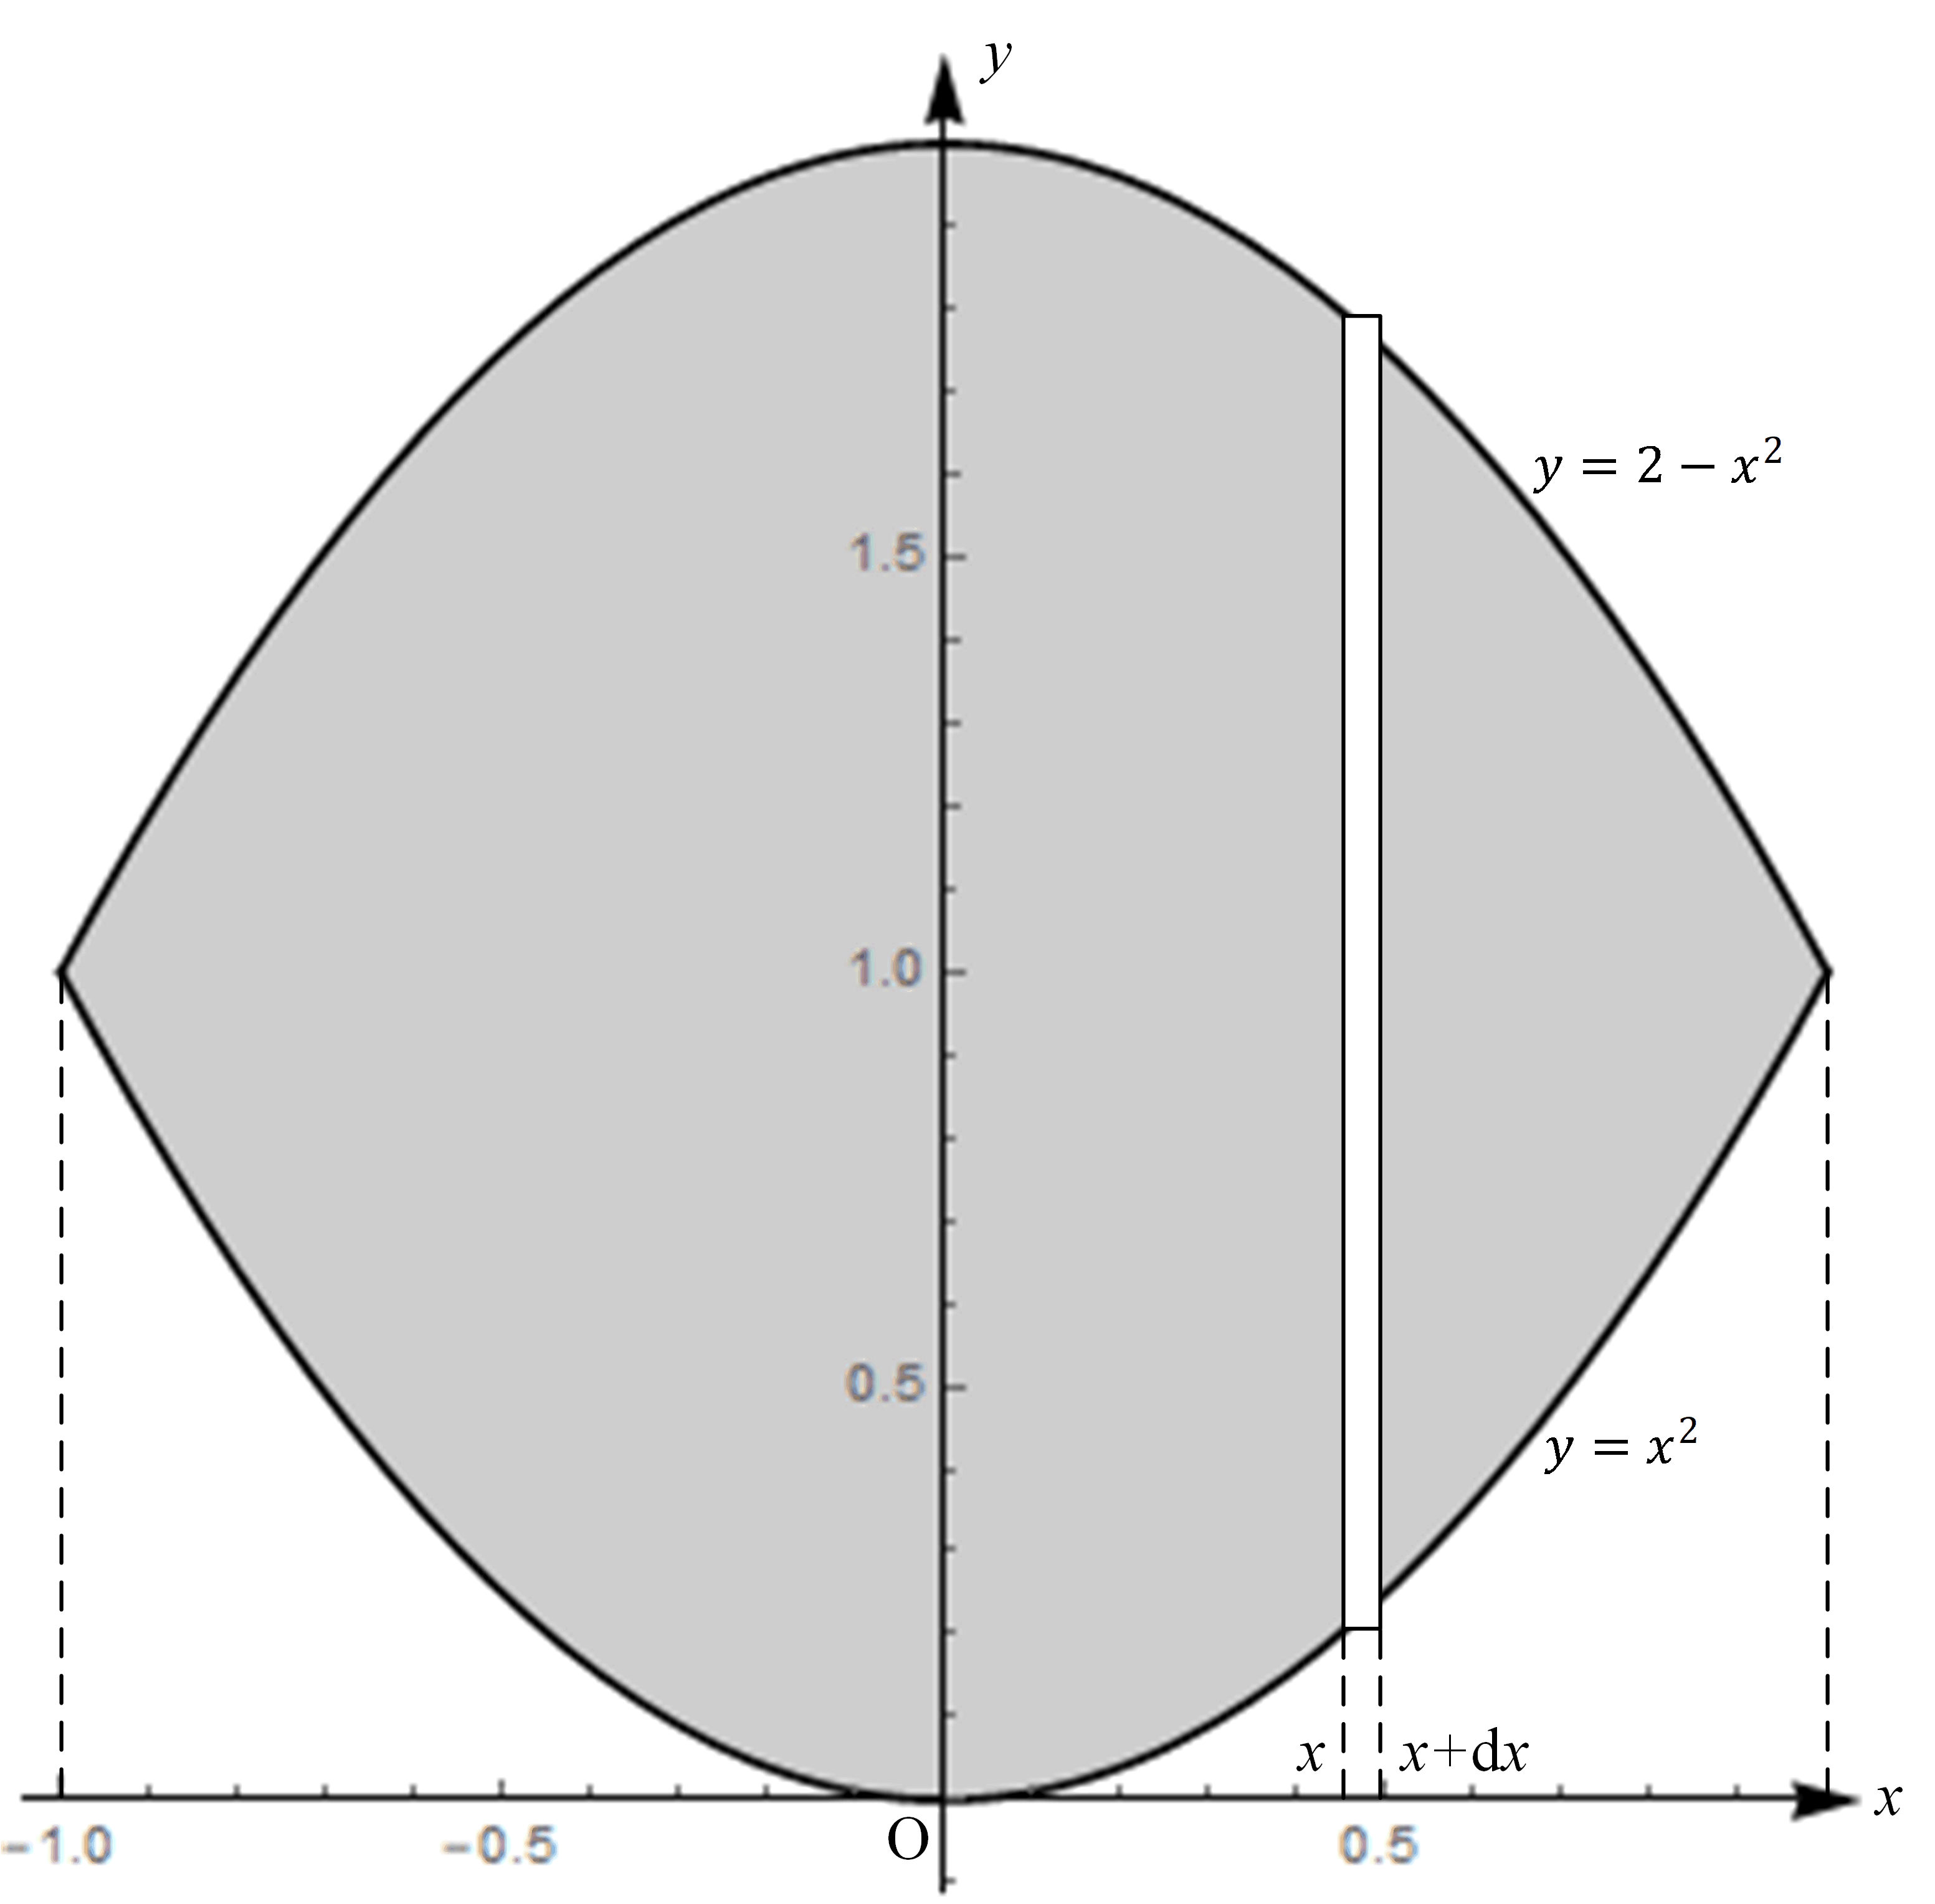
\includegraphics[height=0.3\textheight]{F:/life/2018AutumnTA/Exercises/11/Fig5-1-1.png}
\end{center}
\caption{习题7.5 1.(1)题图示}
\label{5-1-1}
\end{figure}
取图示面积元,图形面积
\[S=\int_{-1}^1(2-x^2-x^2)\mathrm dx=\int_{-1}^1(2-2x^2)\mathrm dx=2x-\frac23x^3\Big|_{-1}^1=4-\frac43=\frac83.\]
(2)各曲线围成的图形如图~\ref{5-1-2}所示,
\begin{figure}[H]
\begin{center}
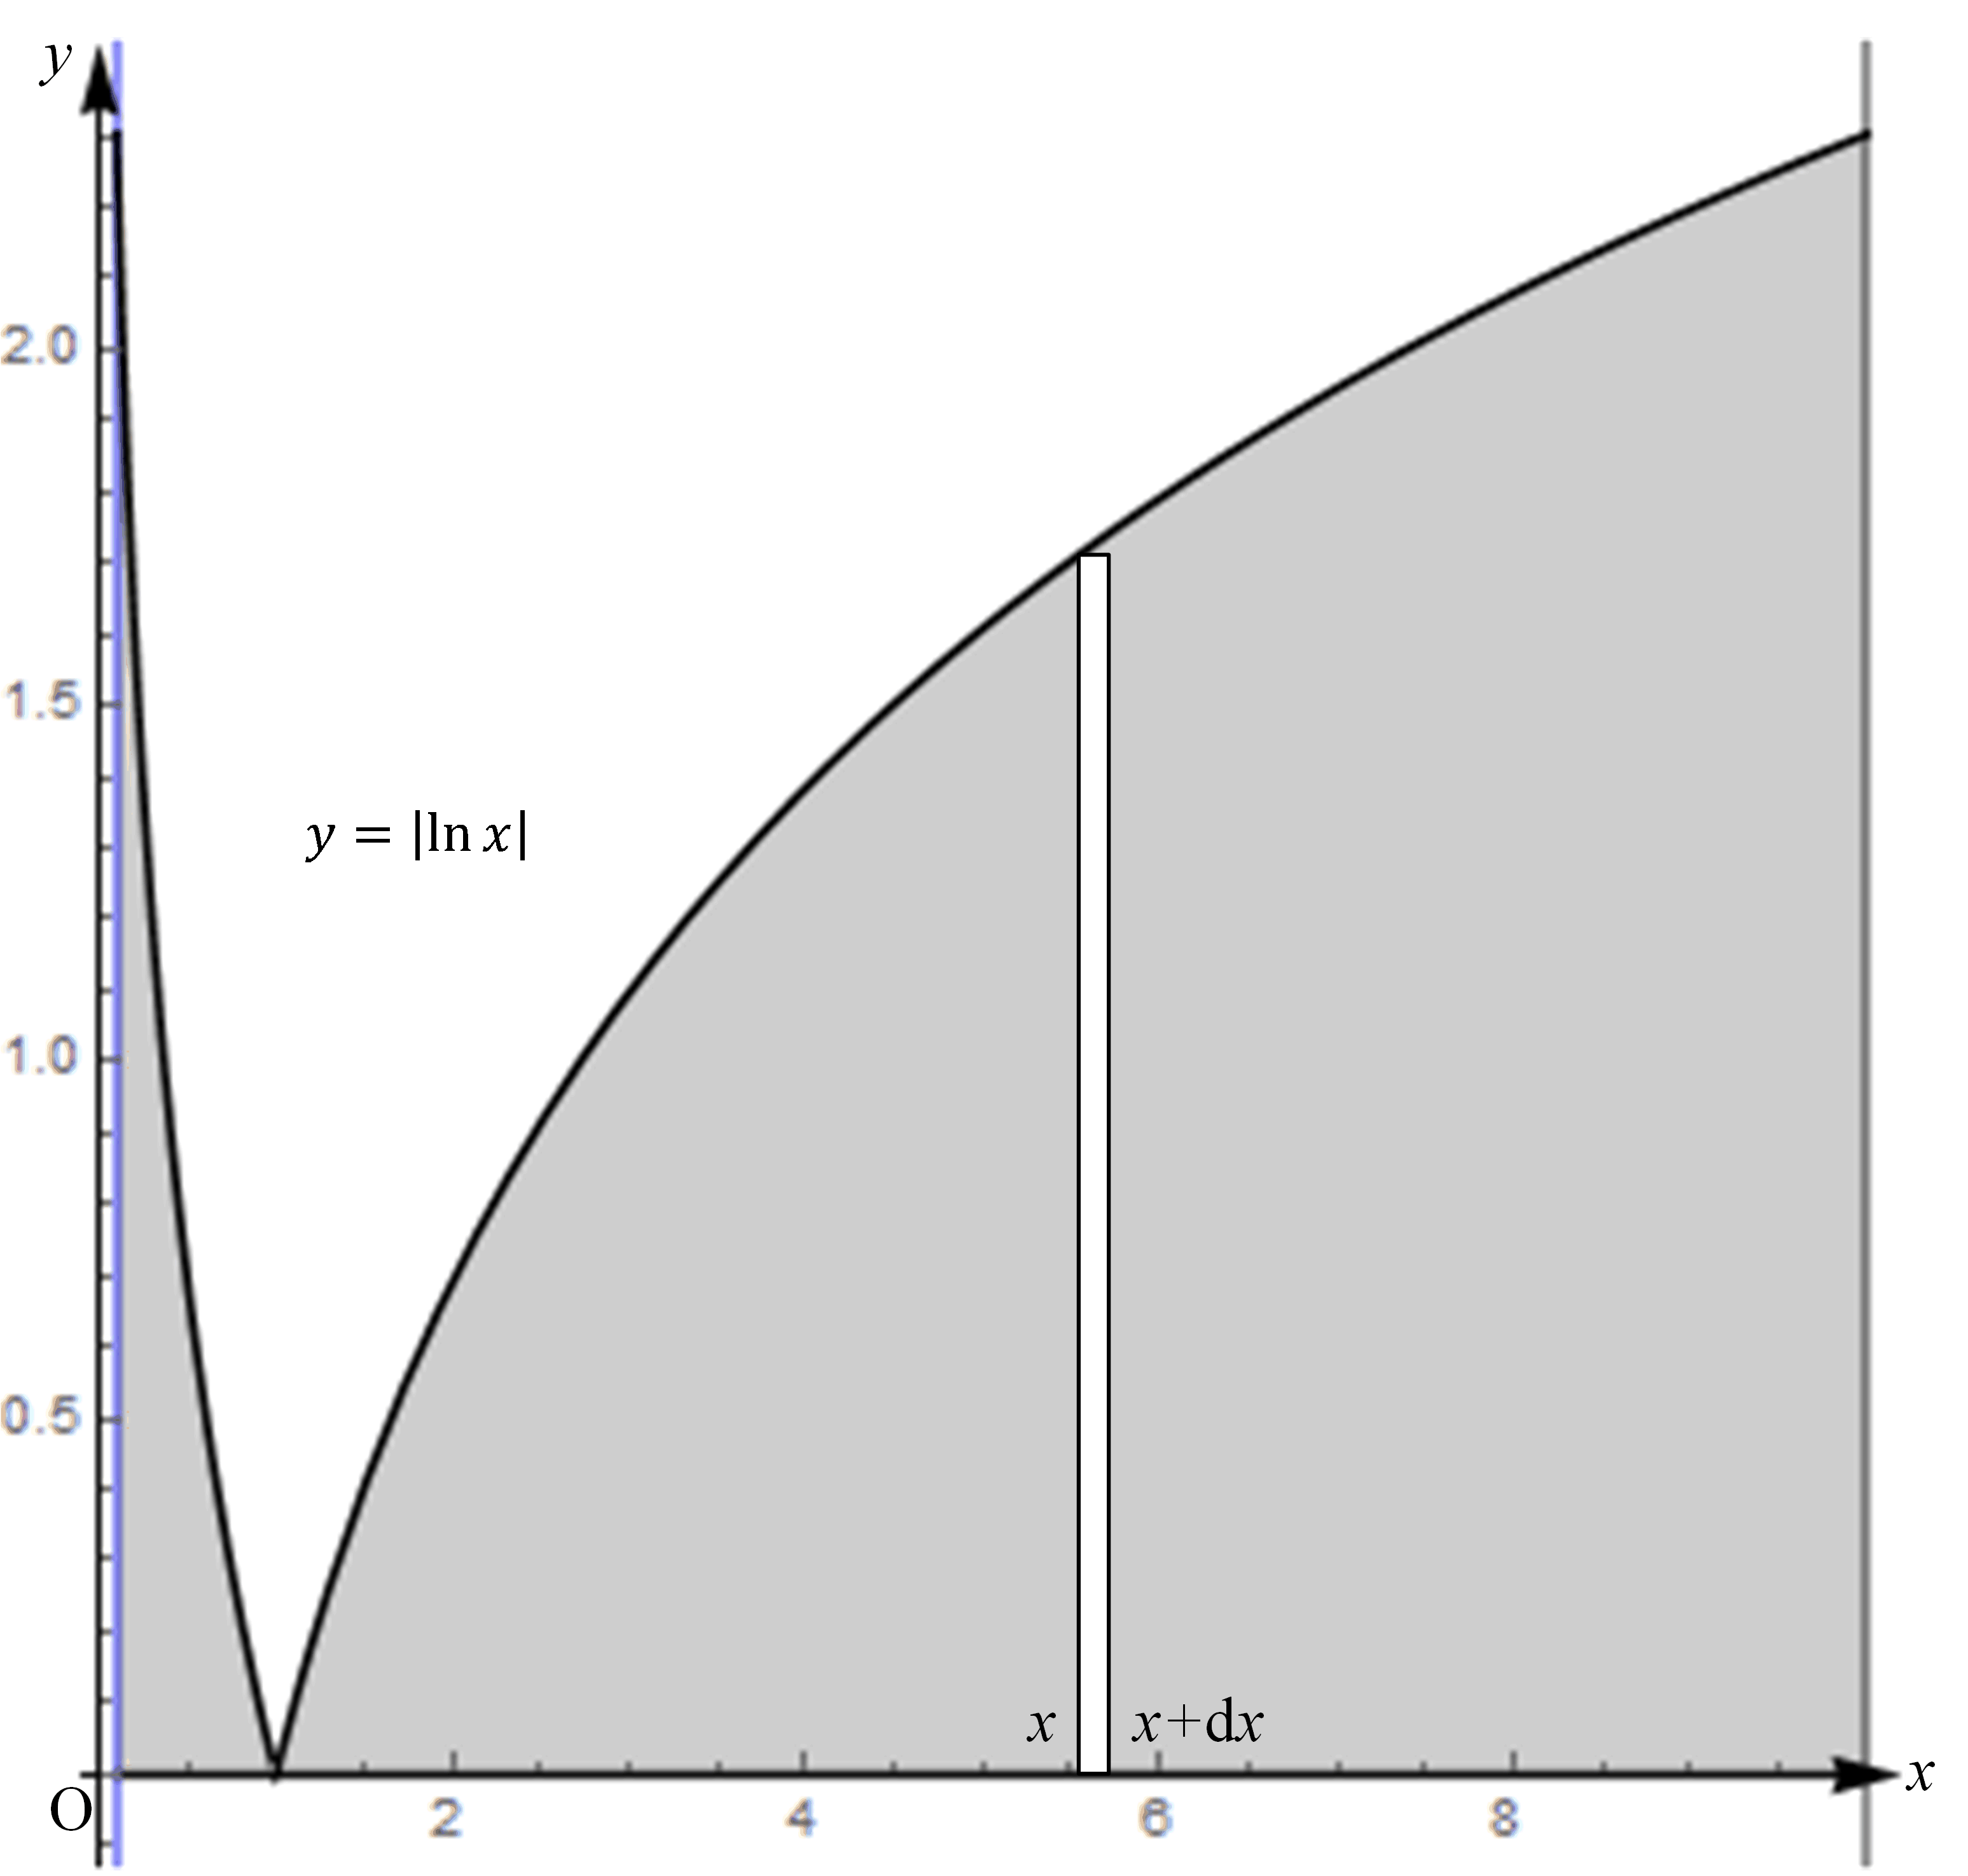
\includegraphics[height=0.3\textheight]{F:/life/2018AutumnTA/Exercises/11/Fig5-1-2.png}
\end{center}
\caption{习题7.5 1.(2)题图示}
\label{5-1-2}
\end{figure}
取图示面积元,图形面积
\[\begin{split}
S&=\int_{\frac1{10}}^{10}|\ln x|\mathrm dx=-\int_{\frac1{10}}^1\ln x\mathrm dx+\int_1^{10}\ln x\mathrm dx=-(x\ln x-x)\Big|_{\frac1{10}}^1+(x\ln x-x)\Big|_1^{10}\\
&=1+(\frac1{10}\ln\frac1{10}-\frac1{10})+10\ln10-10-(-1)=-\frac{81}{10}+\frac{99}{10}\ln10.
\end{split}\]
(3)该曲线围成的图形如图~\ref{5-1-3}所示,
\begin{figure}[H]
\begin{center}
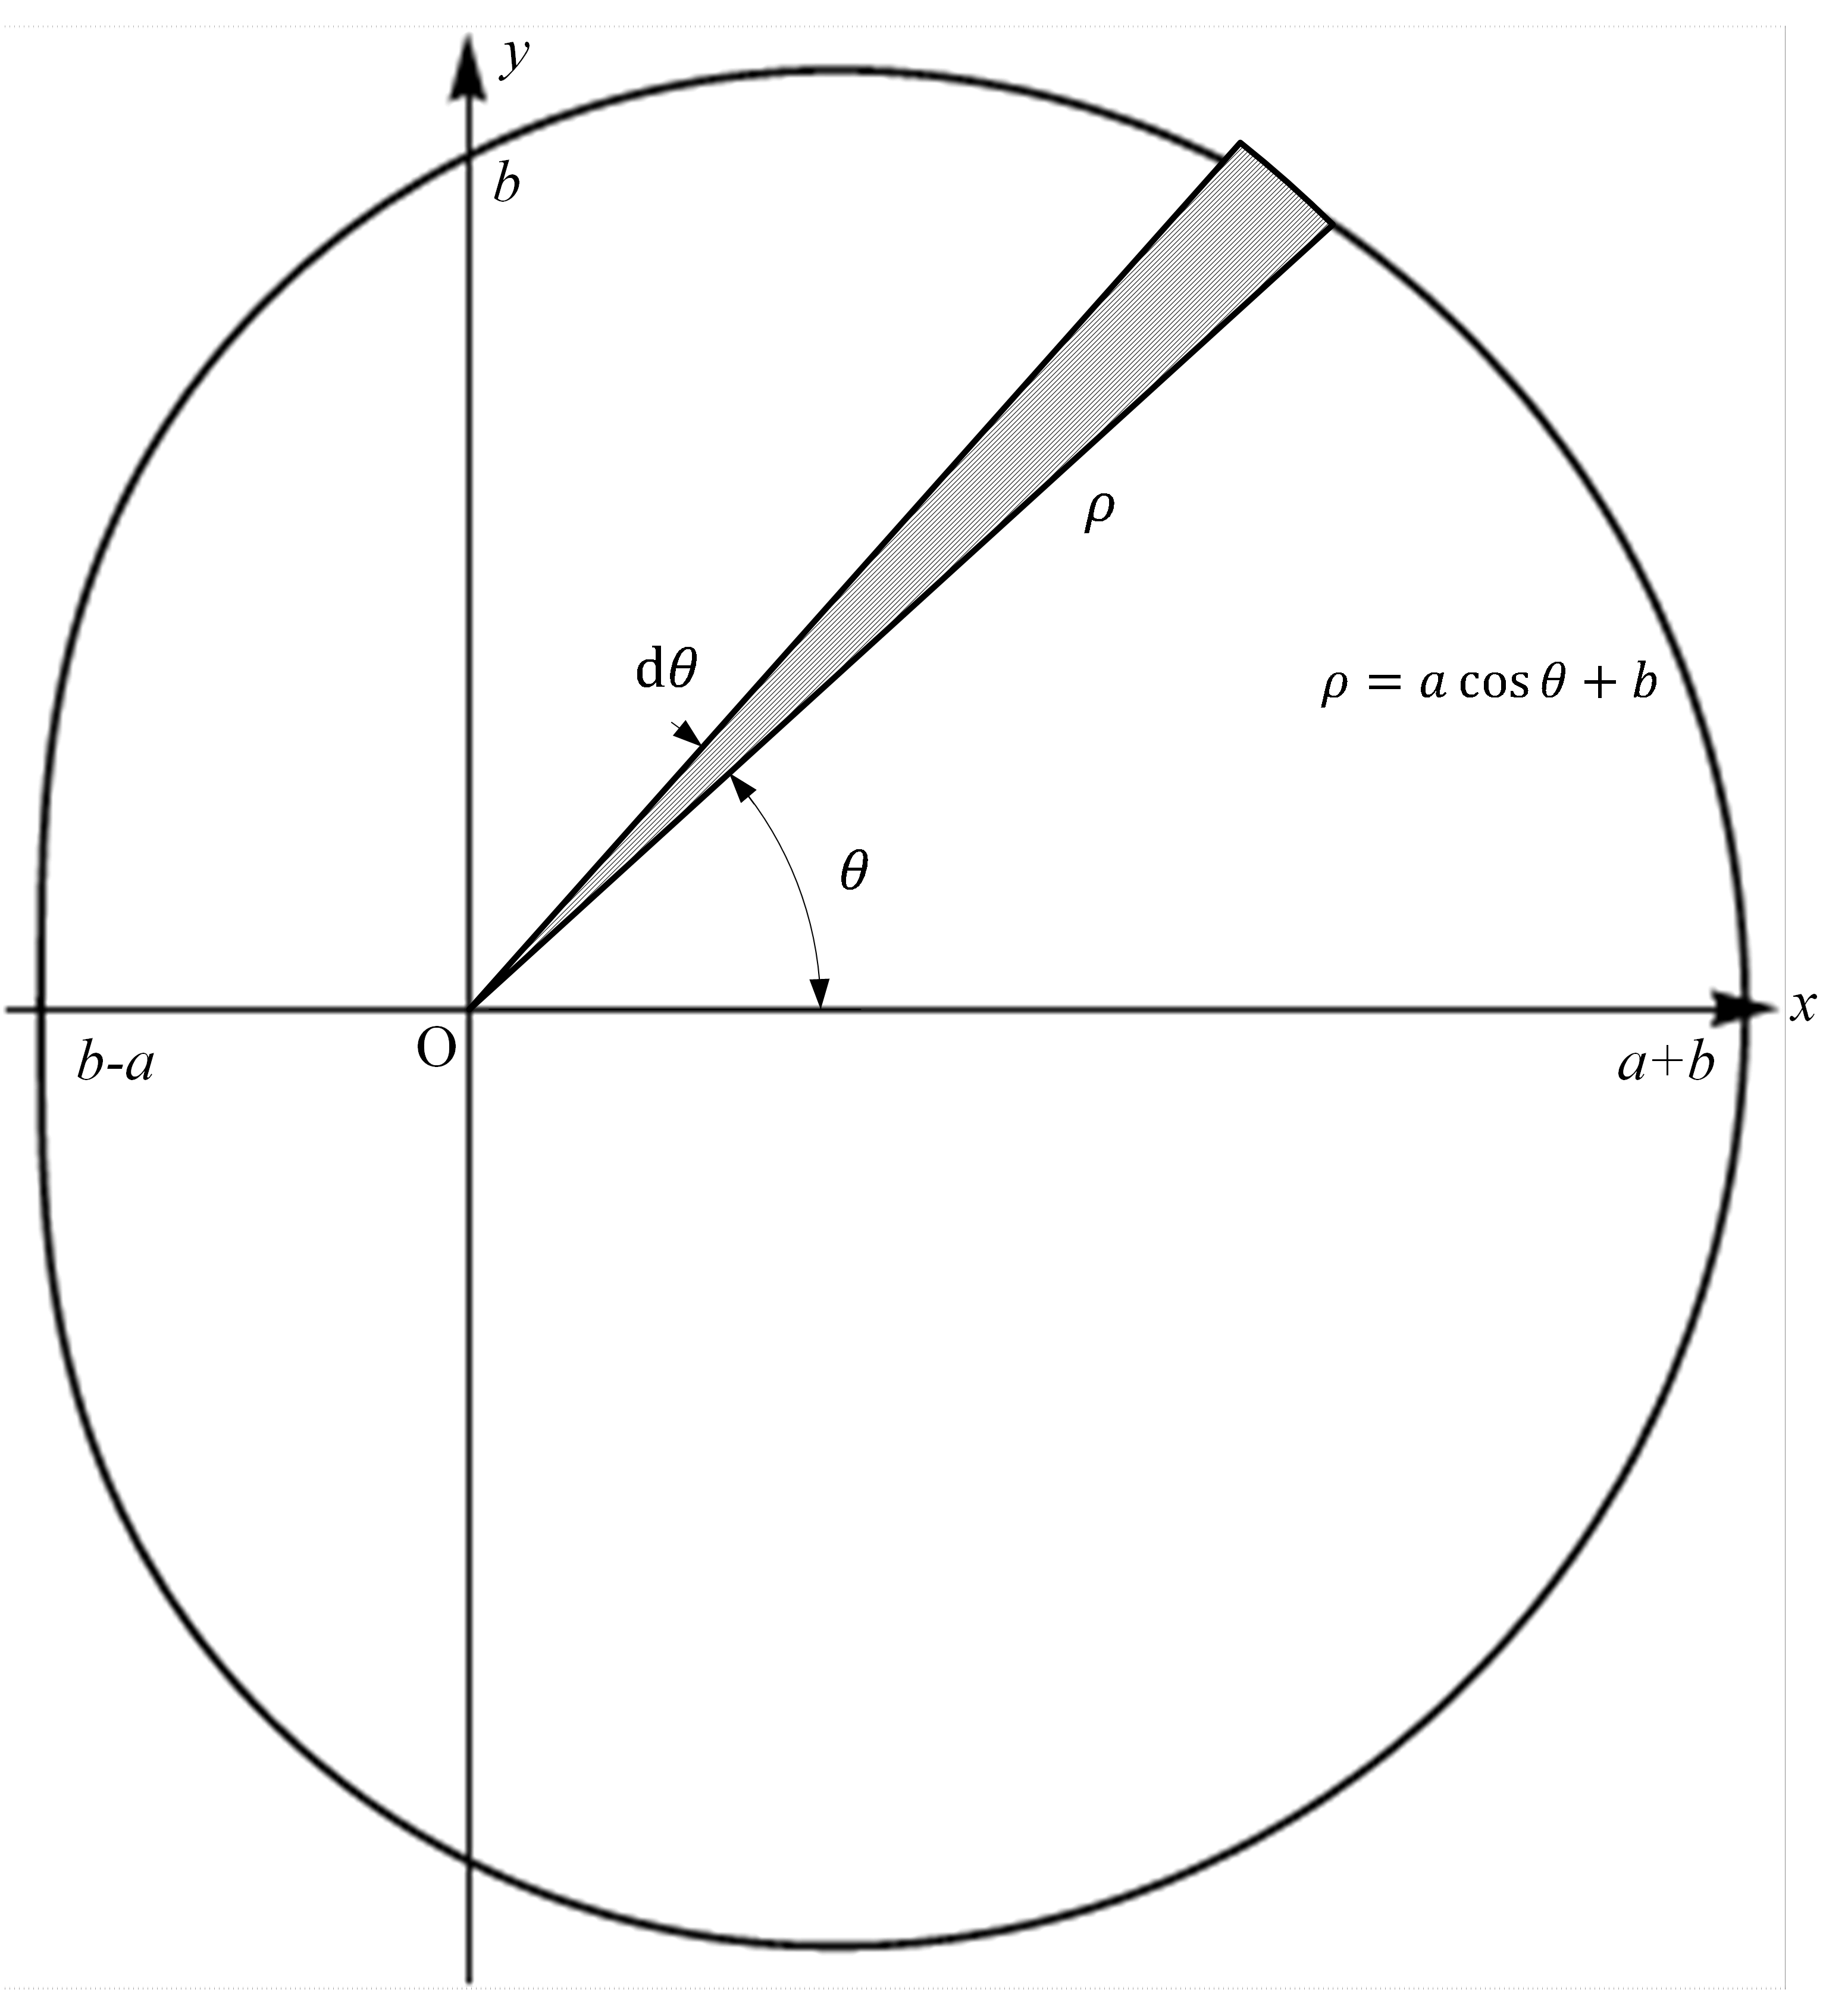
\includegraphics[height=0.35\textheight]{F:/life/2018AutumnTA/Exercises/11/Fig5-1-3.png}
\end{center}
\caption{习题7.5 1.(3)题图示}
\label{5-1-3}
\end{figure}
取图示面积元,图形面积
\[\begin{split}
S&=\int_0^{2\pi}\frac12\rho^2\mathrm d\theta=\int_0^{2\pi}\frac12(a\cos\theta+b)^2\mathrm d\theta=\frac12\int_0^{2\pi}(a^2\cos^2\theta+2ab\cos\theta+b^2)\mathrm d\theta\\
&=\frac12\int_0^{2\pi}[\frac{a^2}2(1+\cos2\theta)+2ab\cos\theta+b^2]\mathrm d\theta=\frac12[\frac12a^2(\theta+\frac12\sin2\theta)+2ab\sin\theta+b^2\theta]_0^{2\pi}\\
&=\frac12[\frac12a^2(2\pi+0)+b^22\pi]=\frac\pi2a^2+\pi b^2.
\end{split}\]
(4)该曲线围成的图形如图~\ref{5-1-4}所示,
\begin{figure}[H]
\begin{center}
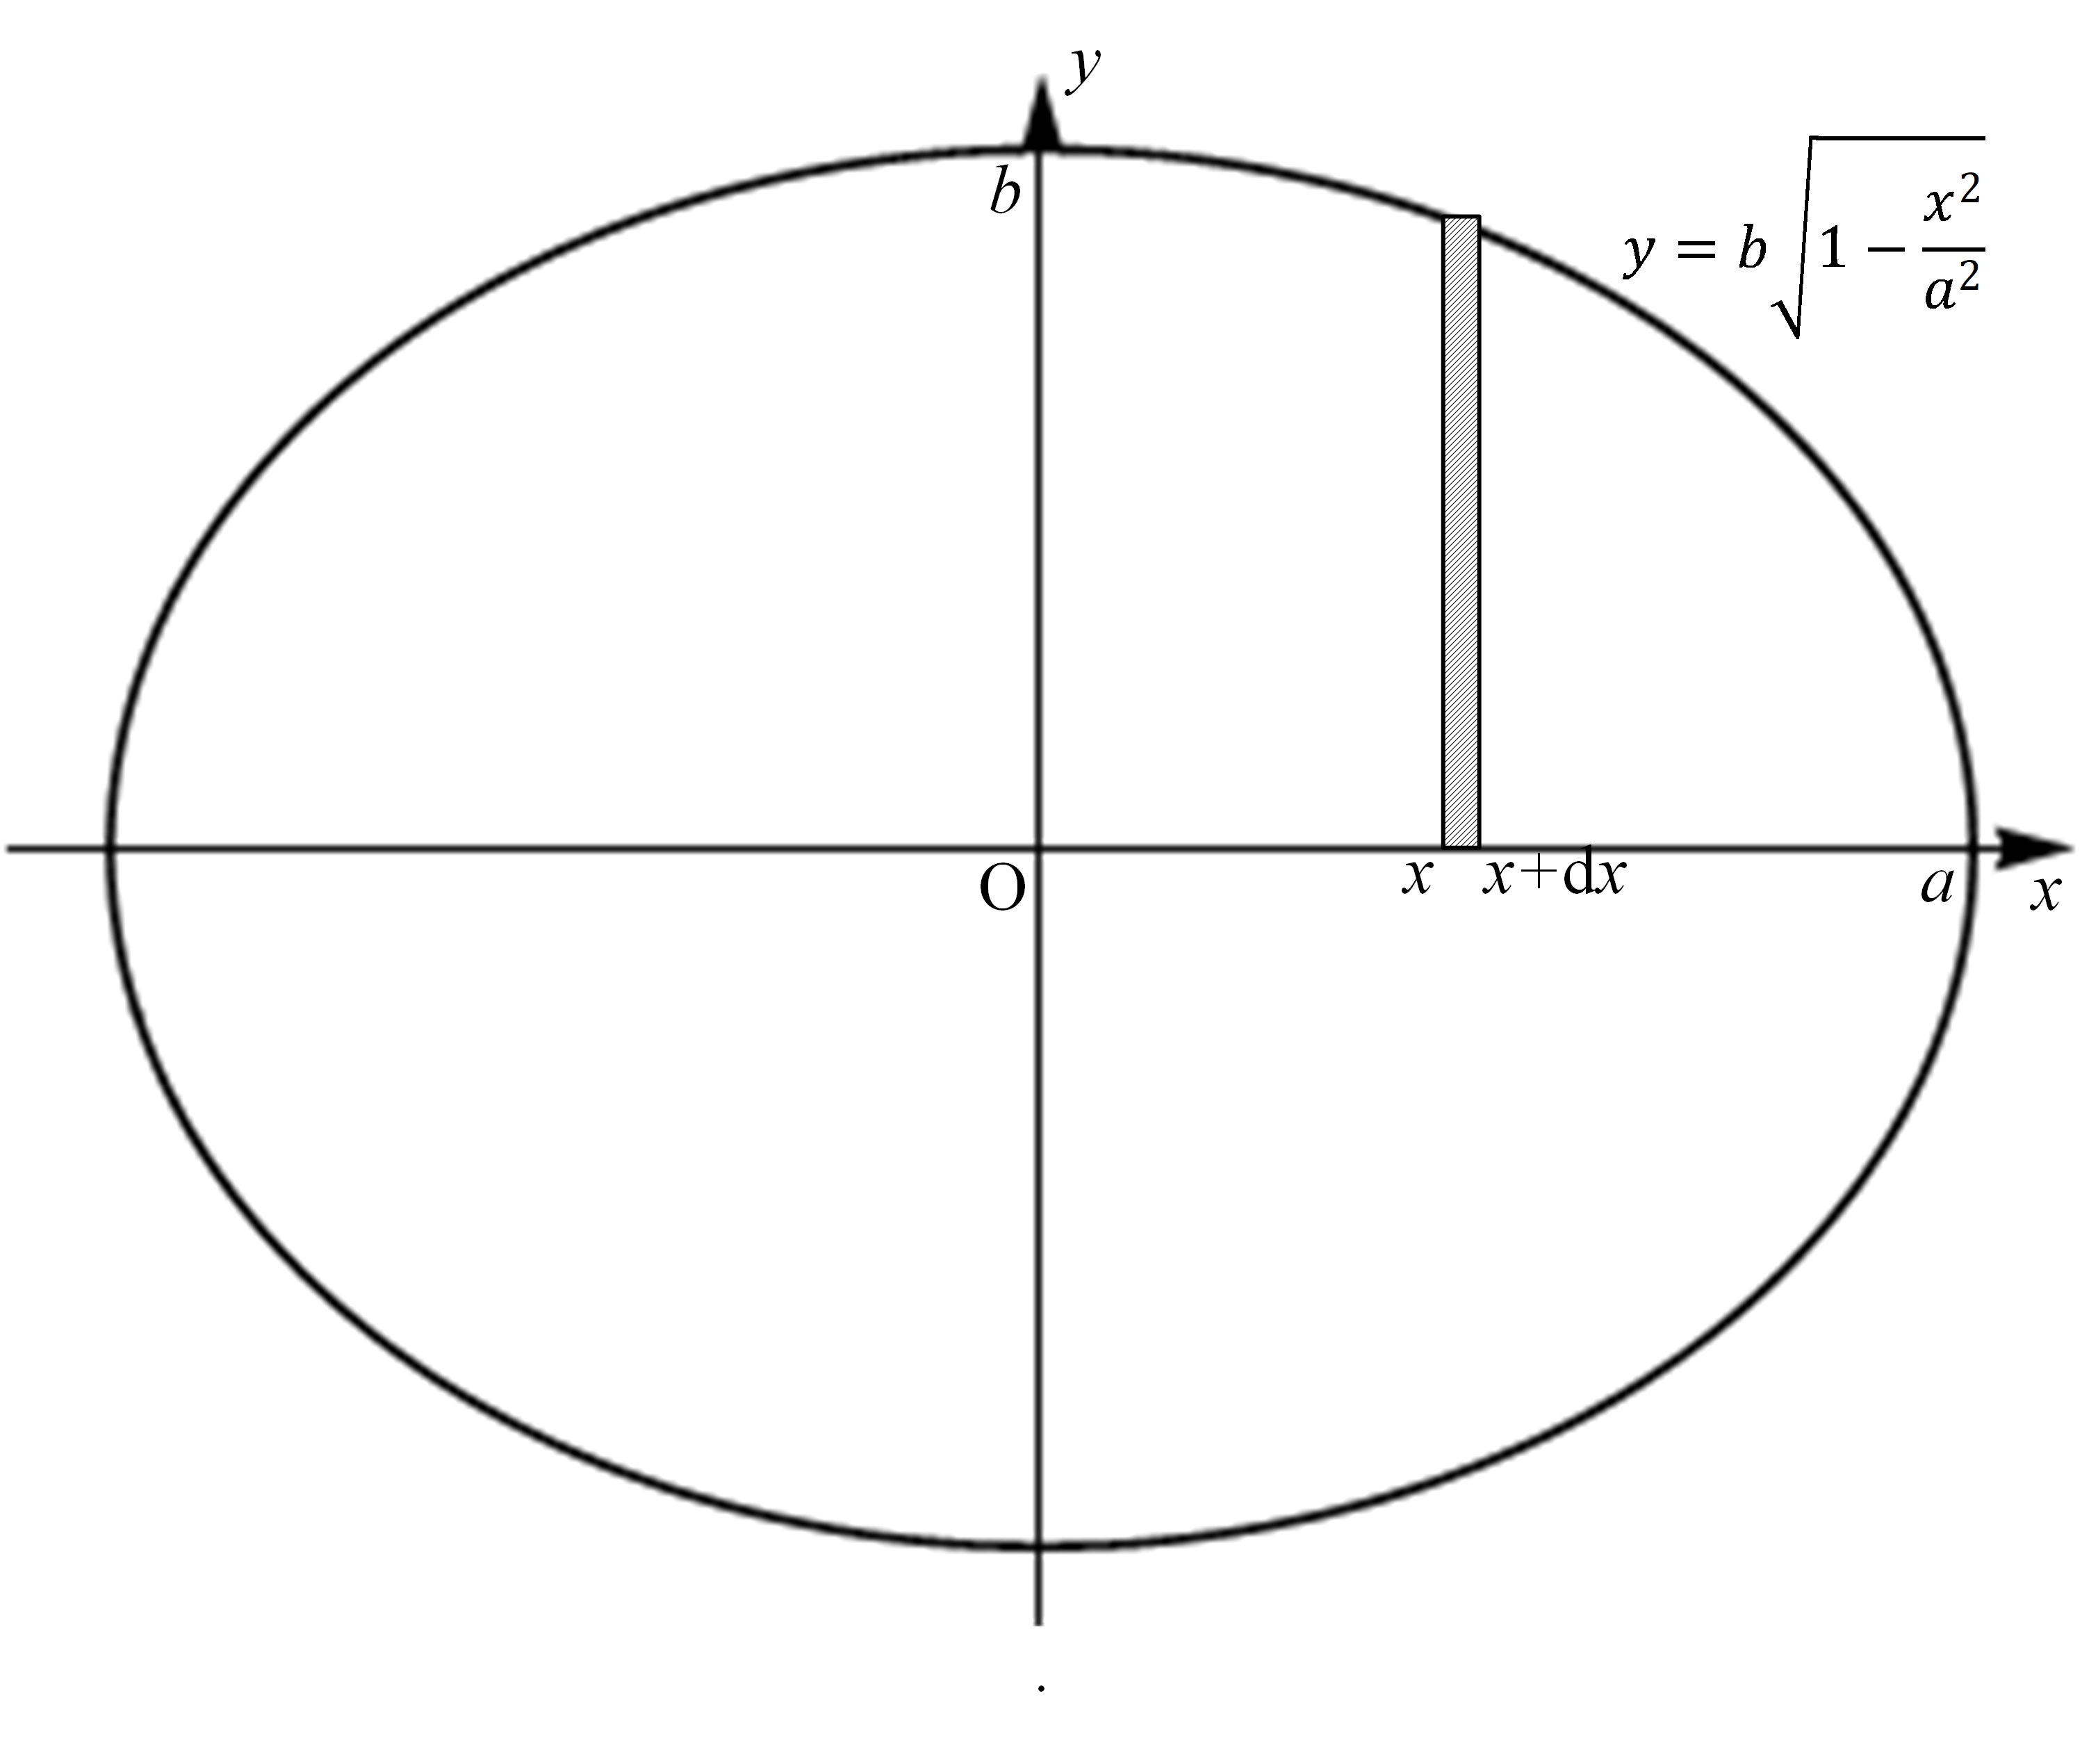
\includegraphics[height=0.25\textheight]{F:/life/2018AutumnTA/Exercises/11/Fig5-1-4.png}
\end{center}
\caption{习题7.5 1.(4)题图示}
\label{5-1-4}
\end{figure}
根据椭圆的对称性,其面积为第一象限部分面积的四倍,取图示面积元,图形面积
\[\begin{split}
S&=4\int_0^ab\sqrt{1-\frac{x^2}{a^2}}\mathrm dx=4\frac ba\int_0^a\sqrt{a^2-x^2}\mathrm dx=4\frac ba\int_0^{\frac\pi2}(a\cos t)(a\cos t)\mathrm dt\\
&=4\frac ba\int_0^{\frac\pi2}a^2\frac{1+\cos2t}2\mathrm dt=2ab\int_0^{\frac\pi2}(1+\cos2t)\mathrm dt=2ab(t+\frac12\sin2t)\Big|_0^\frac\pi2\\
&=\pi ab.
\end{split}\]
(5)由$\sqrt{\frac xa}+\sqrt{\frac yb}=1$知$0\leq x\leq a,0\leq y\leq b$,各曲线围成的图形如图~\ref{5-1-5}所示,
\begin{figure}[H]
\begin{center}
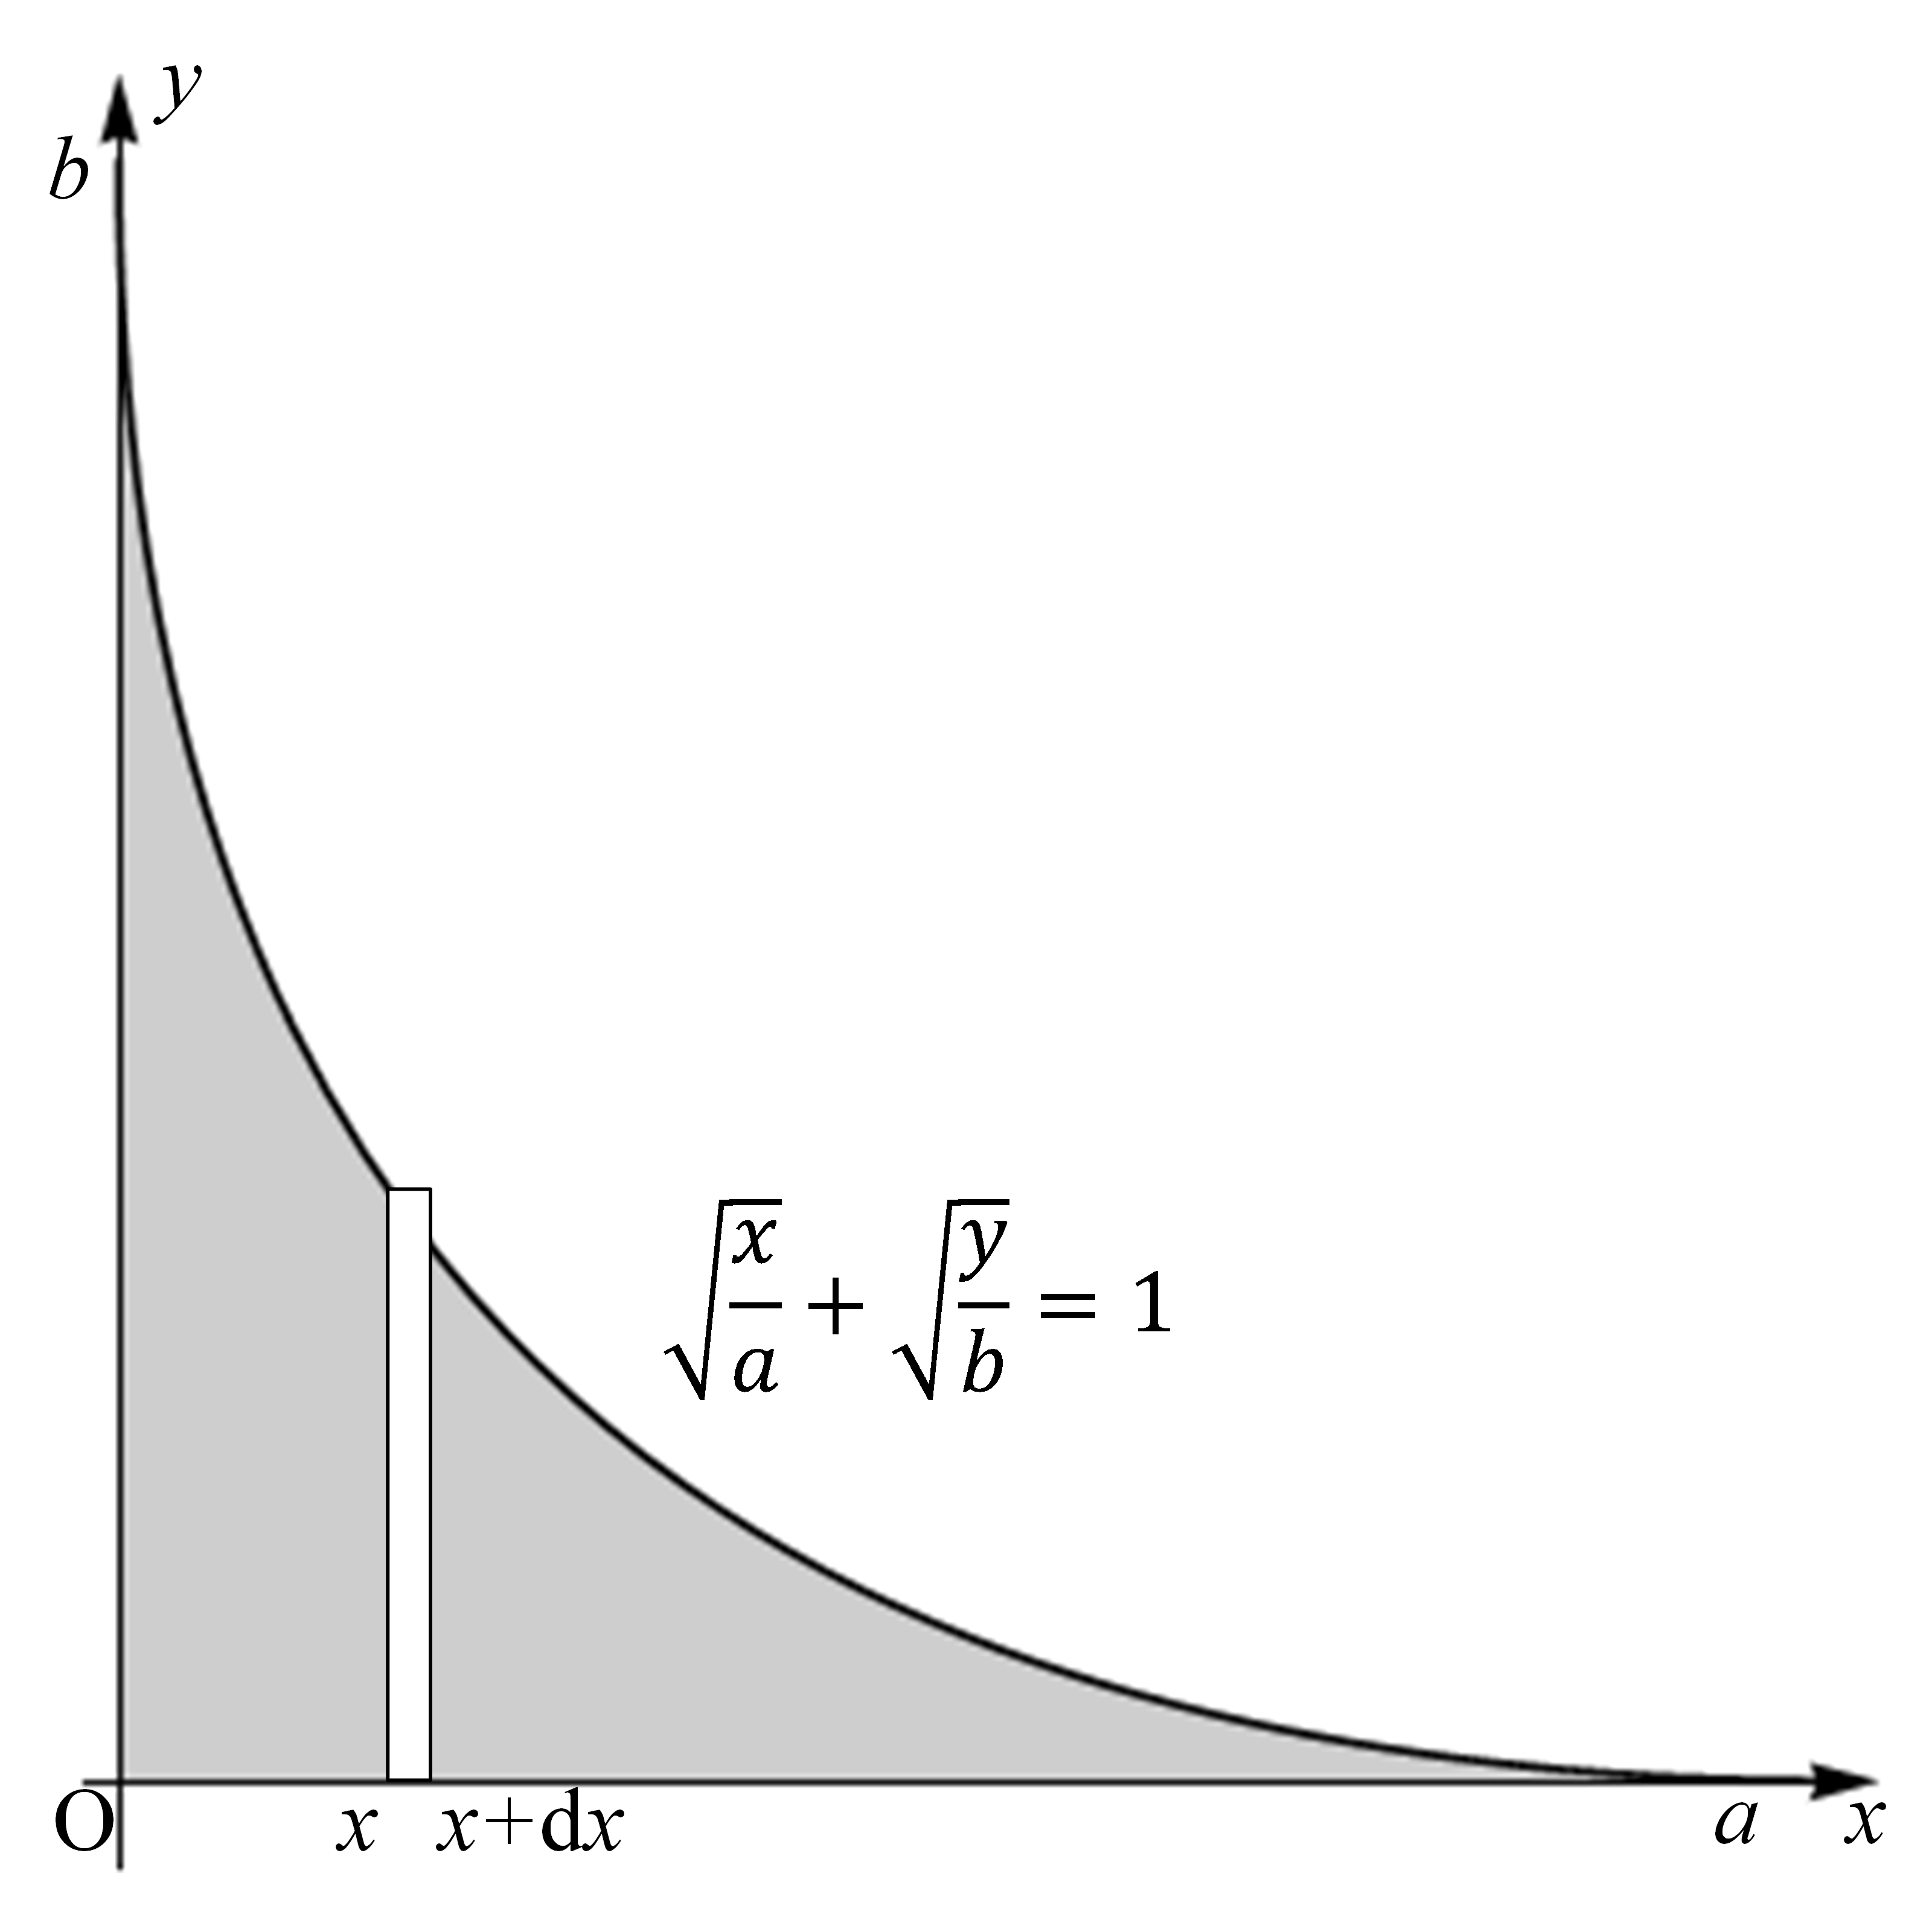
\includegraphics[height=0.3\textheight]{F:/life/2018AutumnTA/Exercises/11/Fig5-1-5.png}
\end{center}
\caption{习题7.5 1.(5)题图示}
\label{5-1-5}
\end{figure}
取图示面积元,图形面积
\[\begin{split}
S&=\int_0^ay\mathrm dx=\int_0^ab(1-\sqrt{\frac xa})^2\mathrm dx=b\int_0^a(1+\frac xa-2\sqrt{\frac xa})\mathrm dx=b[x+\frac 1{2a}x^2-\frac2{\sqrt a}\frac23(\sqrt x)^3]_0^a\\
&=b(a+\frac12a-\frac43a)=\frac16ab.
\end{split}\]
\item求下列曲线的弧长:
\newline
(1)$y=x\sqrt x,0\leq x\leq4$;
\newline
(2)$\sqrt x+\sqrt y=1$;
\newline
(3)圆的渐开线$\begin{cases}
x=a(\cos t+t\sin t),\\
y=a(\sin t-t\cos t),
\end{cases}t\in[0,2\pi]$;
\newline
(4)心脏线$\rho=a(1+\cos\theta),\theta\in[0,2\pi]$.

解:(1)曲线如图~\ref{5-2-1}所示,
\begin{figure}[H]
\begin{center}
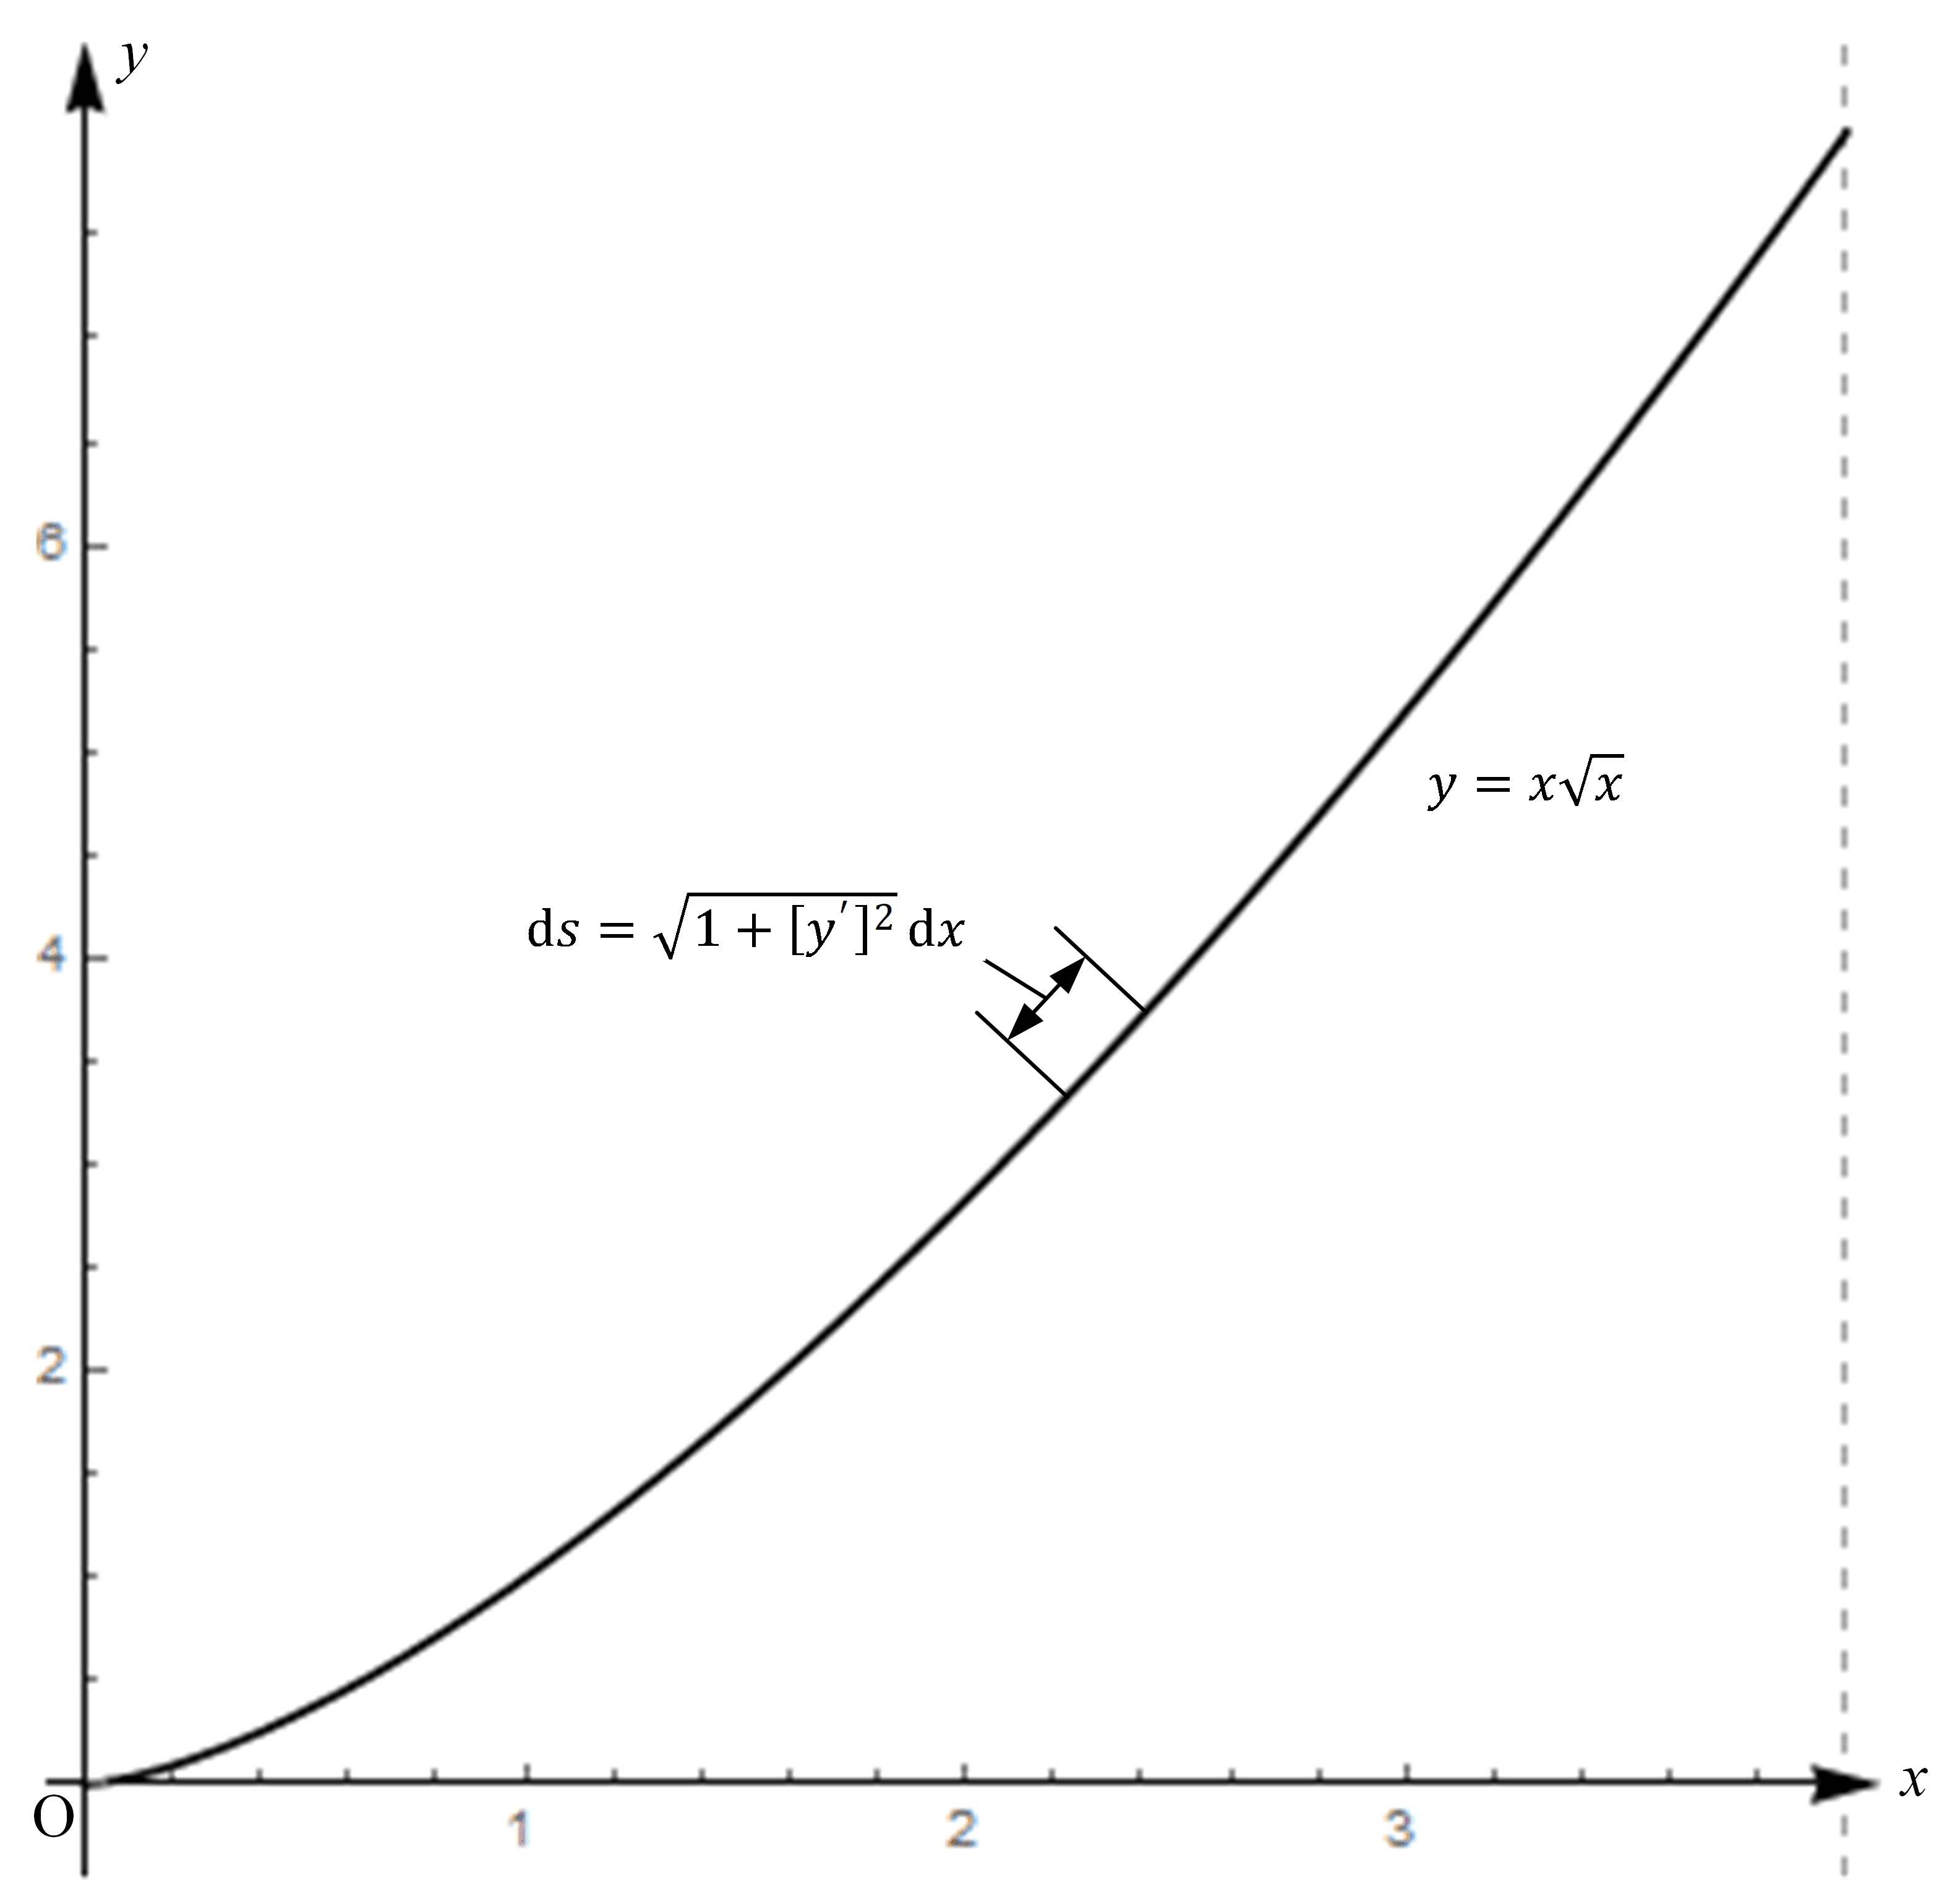
\includegraphics[height=0.4\textheight]{F:/life/2018AutumnTA/Exercises/11/Fig5-2-1.png}
\end{center}
\caption{习题7.5 2.(1)题图示}
\label{5-2-1}
\end{figure}
取图示弧段,曲线长度
\[\begin{split}
l&=\int_0^4\sqrt{1+(y')^2}\mathrm dx=\int_0^4\sqrt{1+(\frac32x^{\frac12})}\mathrm dx=\int_0^4\sqrt{1+\frac94x}\mathrm dx\\
&=\frac49\int_0^4\sqrt{1+\frac94x}\mathrm d(1+\frac94)=\frac49\frac23(1+\frac94x)^{\frac32}\Big|_0^4=\frac8{27}[(1+9)^\frac32-1]=\frac8{27}(10^{\frac32}-1).
\end{split}\]
(2)由$\sqrt x+\sqrt y=1$知$0\leq x\leq1,0\leq y\leq1$,曲线如图~\ref{5-2-2}所示,
\begin{figure}[H]
\begin{center}
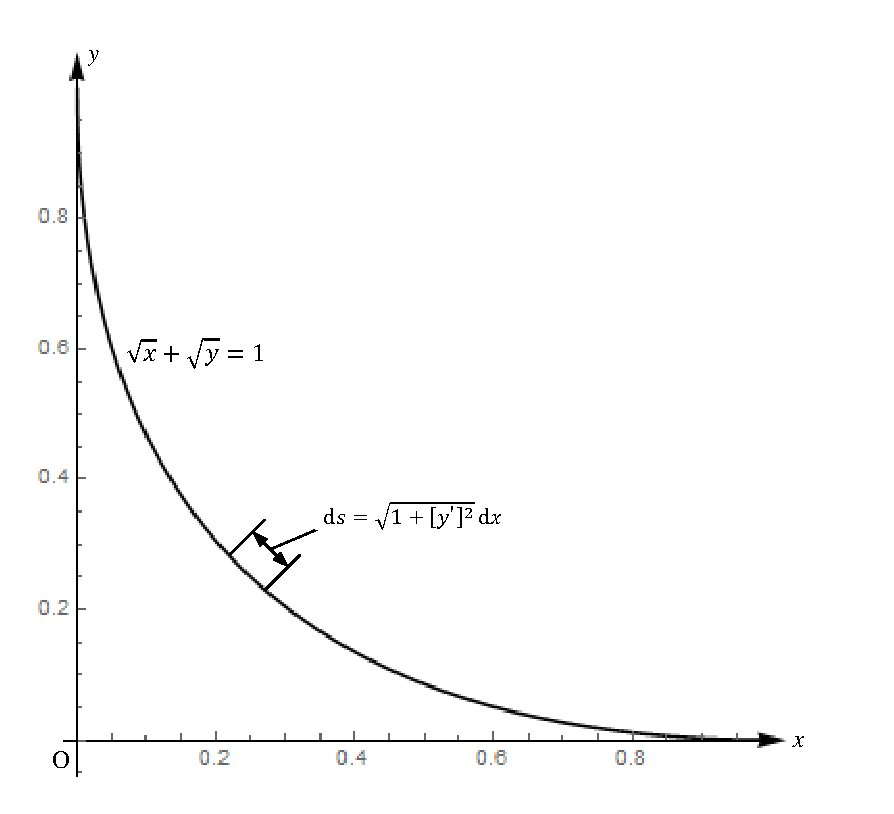
\includegraphics[height=0.4\textheight]{F:/life/2018AutumnTA/Exercises/11/Fig5-2-2.pdf}
\end{center}
\caption{习题7.5 2.(2)题图示}
\label{5-2-2}
\end{figure}
取图示弧段,曲线长度
\[\begin{split}
l&=\int_0^1\sqrt{1+(y')^2}\mathrm dx=\int_0^1\sqrt{1+[2(1-\sqrt x)\frac{-1}{2\sqrt x}]^2}\mathrm dx=\int_0^1\sqrt{1+(\frac{-1}{\sqrt x}+1)^2}\\
&=\int_0^1\sqrt{2+\frac1x-\frac2{\sqrt x}}\mathrm dx\xlongequal{t=\sqrt x}\int_0^1\sqrt{2-\frac2t+\frac1{t^2}}2t\mathrm dt=2\int_0^1\sqrt{2t^2-2t+1}\mathrm dt\\
&=\sqrt2\int_0^1\sqrt{4(t-\frac12)^2+1}\mathrm dt\xlongequal{2(t-\frac12)=\tan u}\sqrt2\int_{-\frac\pi4}^{\frac\pi4}(\sec u)\cdot\frac12\sec^2u\mathrm du=\frac{\sqrt2}2\int_{-\frac\pi4}^{\frac\pi4}\sec^3u\mathrm du\\
&=\frac{\sqrt2}2[\sec u\tan u\Big|_{-\frac\pi4}^{\frac\pi4}-\int_{-\frac\pi4}^{\frac\pi4}\tan u\tan \sec u\mathrm du]=2-\frac{\sqrt2}2\int_{-\frac\pi4}^{\frac\pi4}(\sec^2u-1)\sec u\mathrm du\\
&=2-\frac{\sqrt2}2\int_{-\frac\pi4}^{\frac\pi4}(\sec^3u-\sec u)\mathrm du=\frac12(2+\frac{\sqrt2}2\int_{-\frac\pi4}^{\frac\pi4}\sec u\mathrm du)=\frac12[2+\frac{\sqrt 2}2\ln(\sec u+\tan u)\Big|_{-\frac\pi4}^{\frac\pi4}]\\
&=\frac12\{2+\frac{\sqrt2}2[\ln(\sqrt 2+1)-\ln{\sqrt 2-1}]\}=1+\frac{\sqrt2}4\ln\frac{\sqrt2+1}{\sqrt2-1}=1+\frac{\sqrt2}2\ln(\sqrt2+1).
\end{split}\]
(3)曲线如图~\ref{5-2-3}所示,
\begin{figure}[H]
\begin{center}
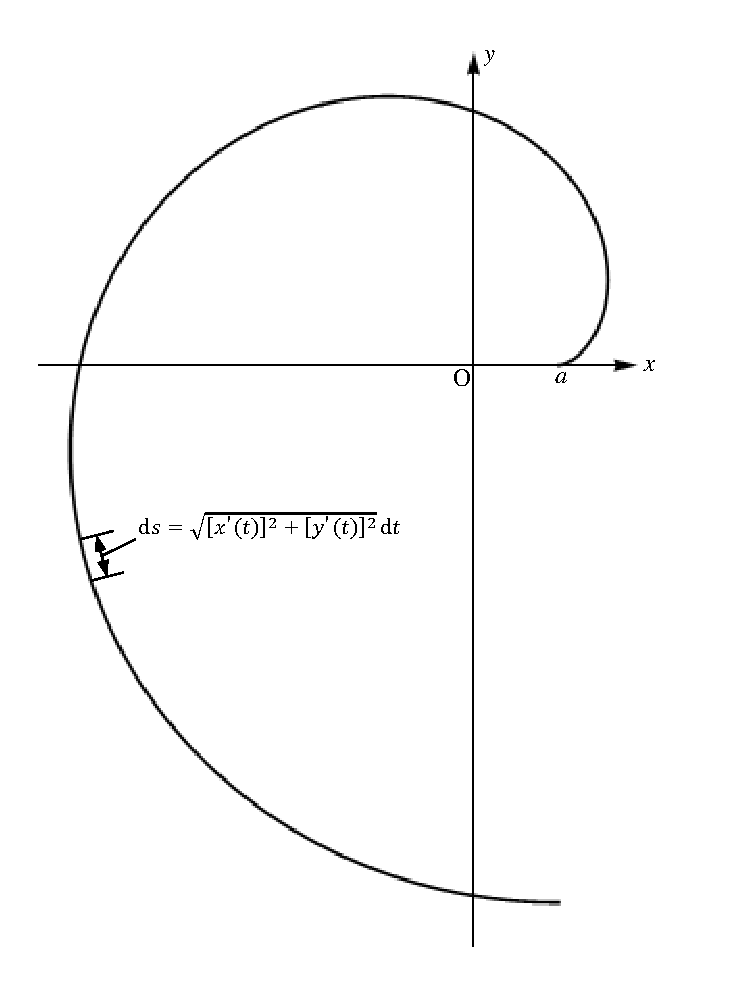
\includegraphics[height=0.5\textheight]{F:/life/2018AutumnTA/Exercises/11/Fig5-2-3.pdf}
\end{center}
\caption{习题7.5 2.(3)题图示}
\label{5-2-3}
\end{figure}
取图示弧段,曲线长度
\[l=\int_0^{2\pi}\sqrt{[x'(t)]^2+[y'(t)]^2}\mathrm dt=\int_0^{2\pi}\sqrt{a^2(t\cos t)^2+a^2(t\sin t)^2}\mathrm dt=a\int_0^{2\pi}t\mathrm dt=\frac a2t^2\Big|_0^{2\pi}
=2a\pi^2.\]
(4)曲线如图~\ref{5-2-4}所示,
\begin{figure}[H]
\begin{center}
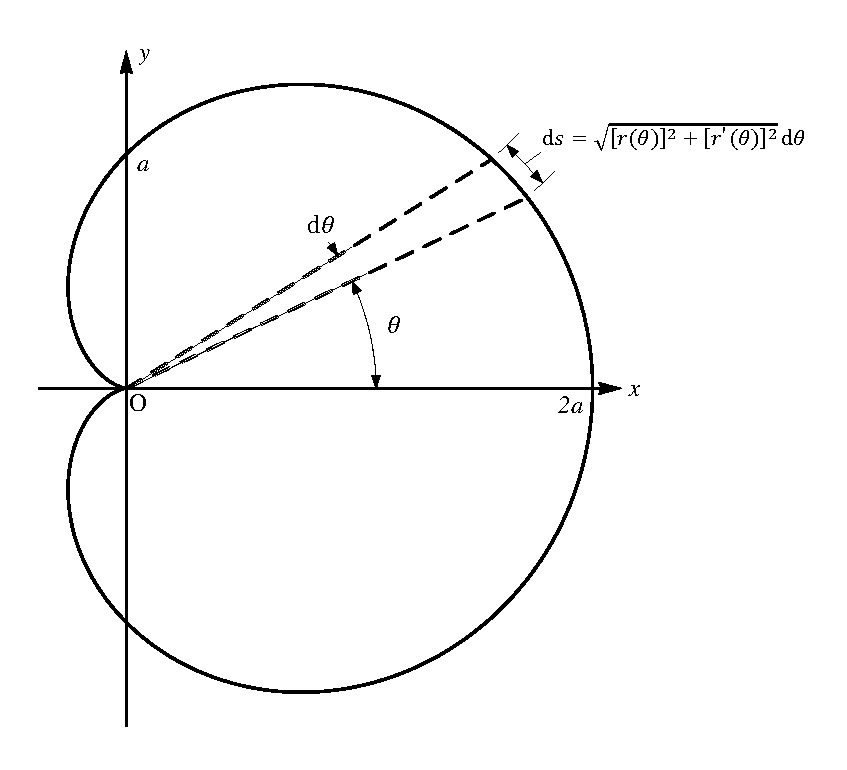
\includegraphics[height=0.4\textheight]{F:/life/2018AutumnTA/Exercises/11/Fig5-2-4.pdf}
\end{center}
\caption{习题7.5 2.(4)题图示}
\label{5-2-4}
\end{figure}
取图示弧段,曲线长度
\[\begin{split}
l&=\int_0^{2\pi}\sqrt{[r(\theta)]^2+[r'(\theta)]^2}\mathrm d\theta=\int_0^{2\pi}\sqrt{a^2(1+\cos\theta)^2+a^2(-\sin\theta)^2}\mathrm d\theta\\
&=a\int_0^{2\pi}\sqrt{(1+\cos\theta)^2+(-\sin\theta)^2}\mathrm d\theta=a\int_0^{2\pi}\sqrt{2+2\cos\theta}\mathrm d\theta\\
&=a\int_0^{2\pi}\sqrt{4\cos^2\frac\theta2}\mathrm d\theta=2a\int_0^{2\pi}|\cos\frac\theta2|\mathrm d\theta\\
&=2a(\int_{0}^{\pi}\cos\frac\theta2\mathrm d\theta-\int_{\pi}^{2\pi}\cos\frac\theta2\mathrm d\theta)\\
&=4a\int_{0}^{\pi}\cos\frac\theta2\mathrm d\theta=8a\sin\frac\theta2\Big|_0^\pi=8a.
\end{split}\]
\item求下列曲线的曲率及曲率半径:
\newline
(1)抛物线$y^2=2px,p>0$;
\newline
(2)旋轮线$\begin{cases}
x=a(t-\sin t),\\
y=a(1-\cos t),
\end{cases},a>0$;
\newline
(3)双纽线$\rho^2=2a^2\cos2\theta,a>0$.

解:(1)如图~\ref{5-3-1}所示,
\begin{figure}[H]
\begin{center}
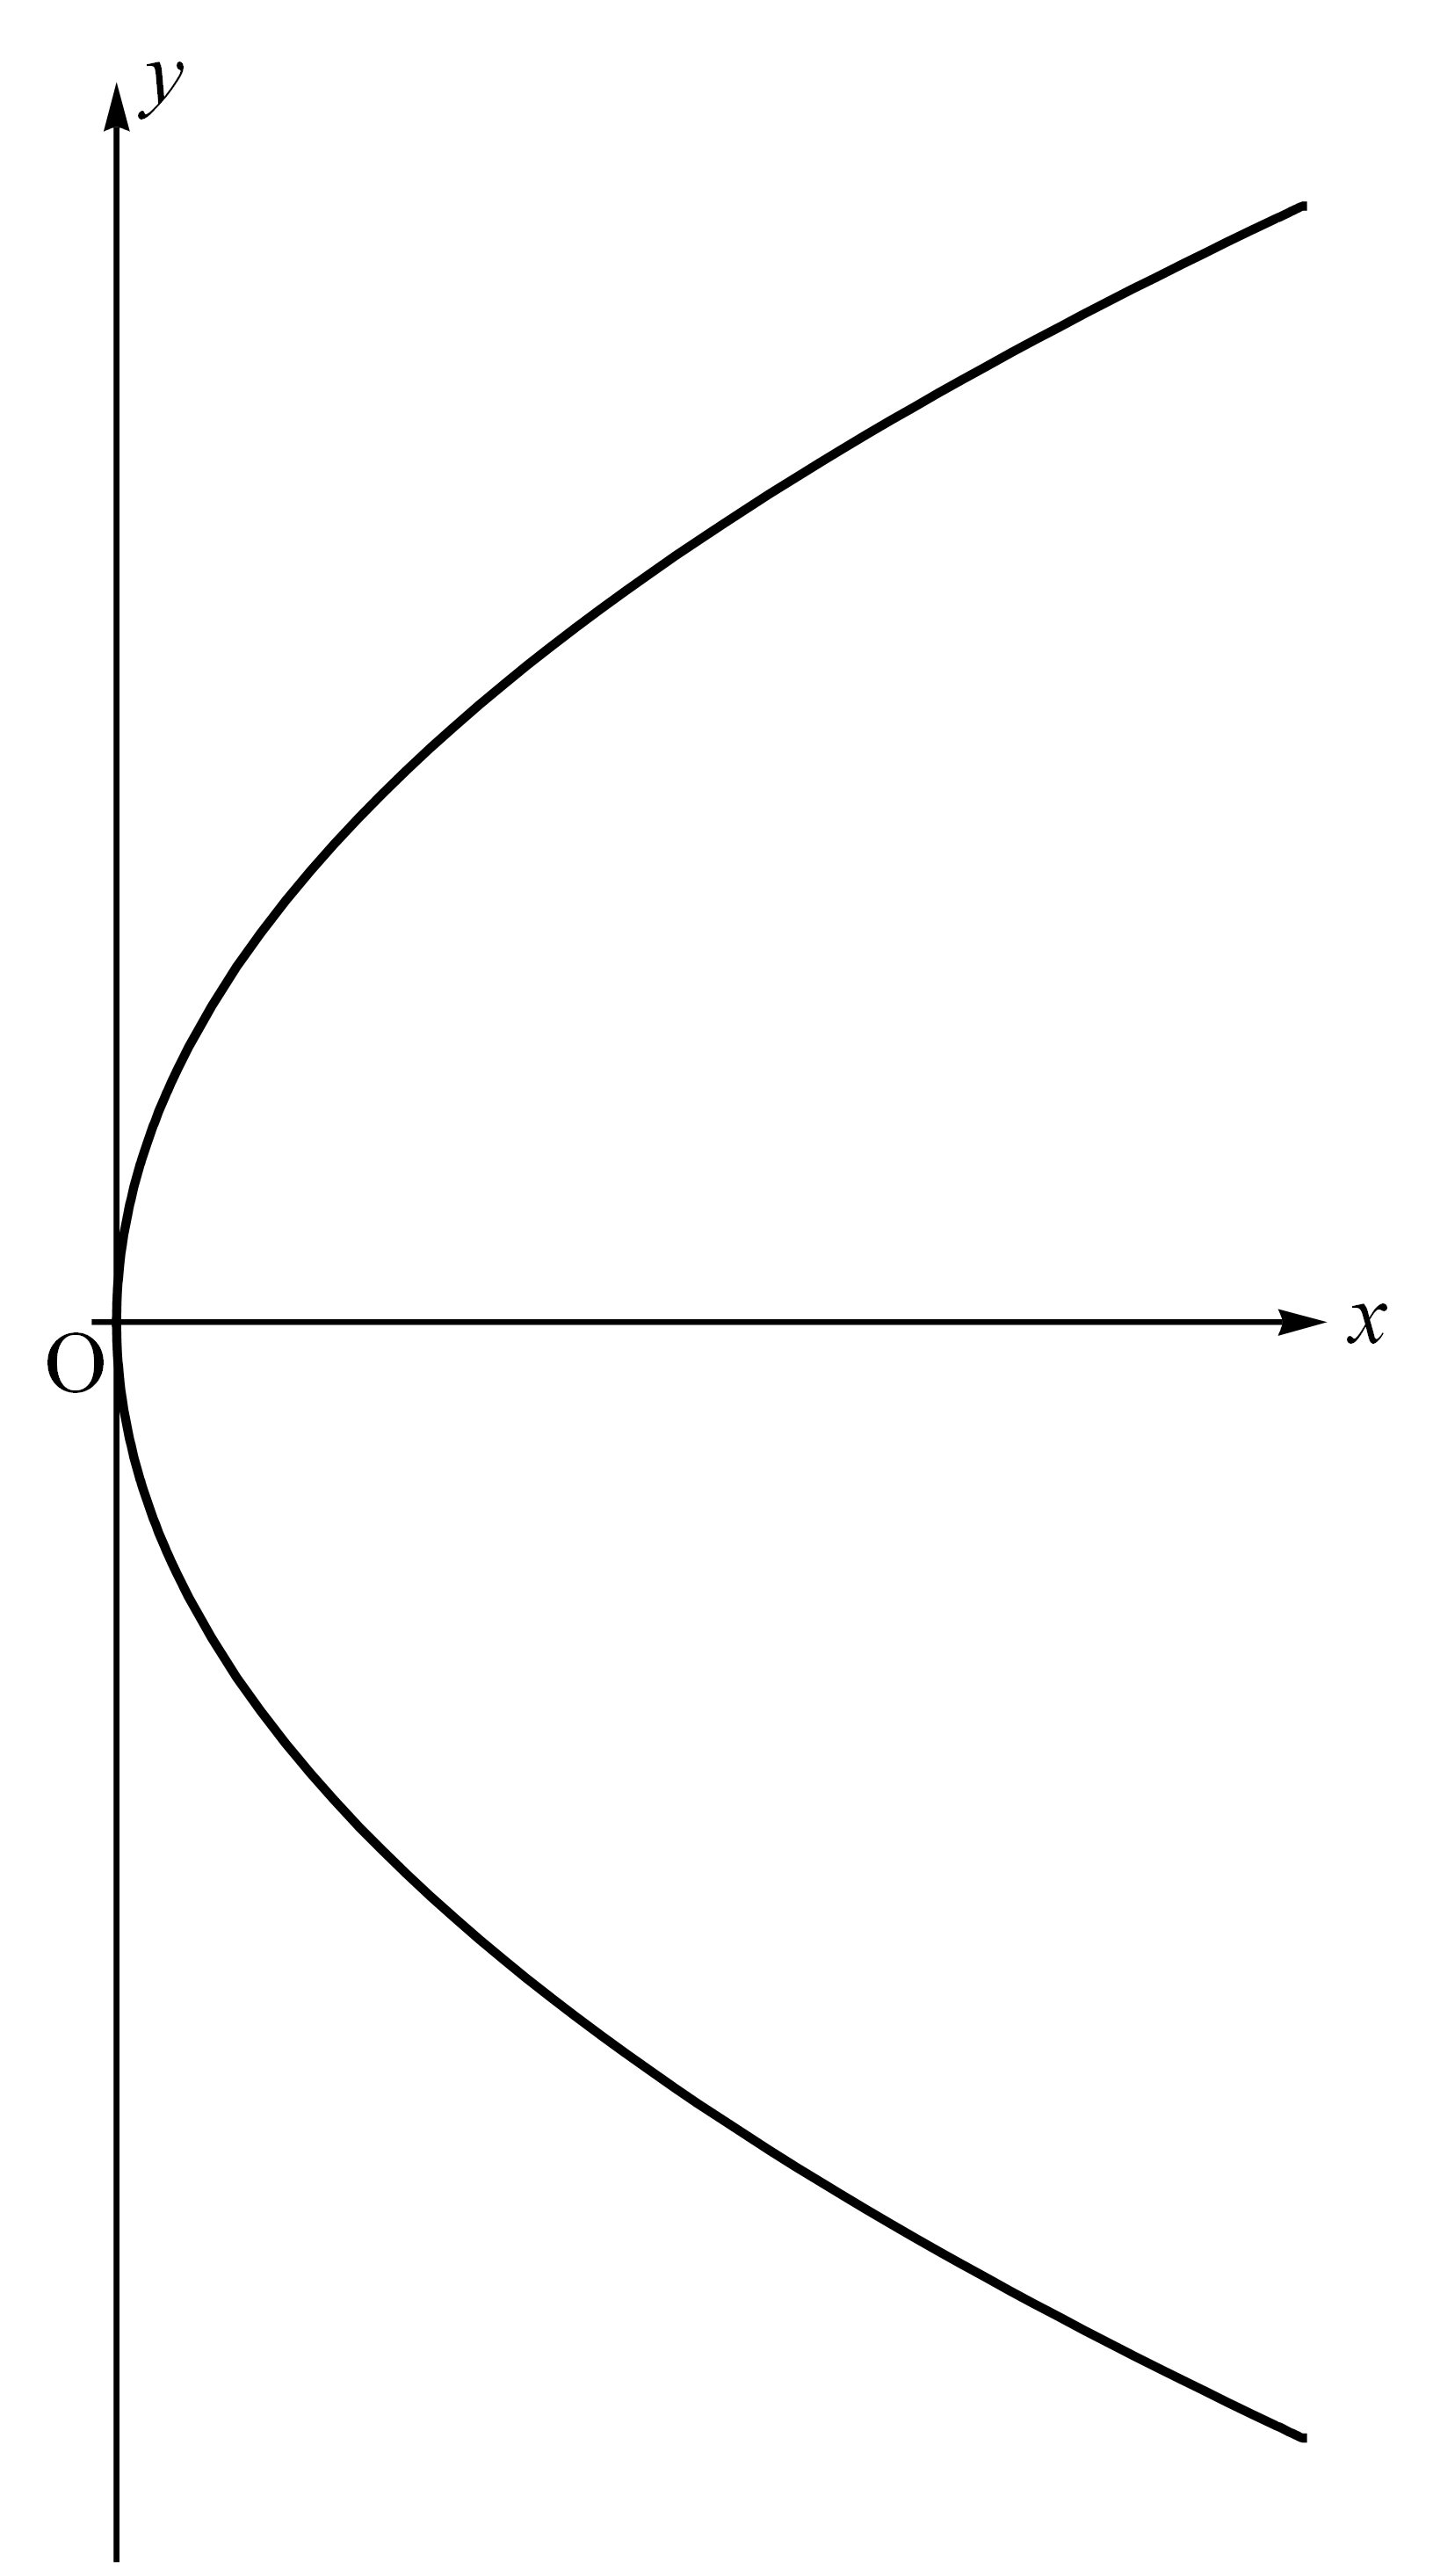
\includegraphics[height=0.4\textheight]{F:/life/2018AutumnTA/Exercises/11/Fig5-3-1.png}
\end{center}
\caption{习题7.5 3.(1)题图示}
\label{5-3-1}
\end{figure}
将$y^2=2px$两边对$x$求导得$2yy'=2p$,故$y'=\frac{p}y$

$\therefore y''=\frac{-py'}{y^2}=-\frac{p^2}{y^3}$

$\therefore$曲率$k=\frac{|y''|}{[1+(y')^2]^{\frac32}}=\frac{|-\frac{p^2}{y^3}|}{[1+(\frac{p}y)^2]^{\frac32}}=\frac{p^2}{(y^2+p^2)^{\frac32}}=\frac{p^2}{(2px+p^2)^{\frac32}}=\frac{\sqrt p}{(2x+p)^{\frac32}}$

曲率半径$R=\frac1k=\frac{(2x+p)^{\frac32}}{\sqrt p}$.

(2)如图~\ref{5-3-2}所示,
\begin{figure}[H]
\begin{center}
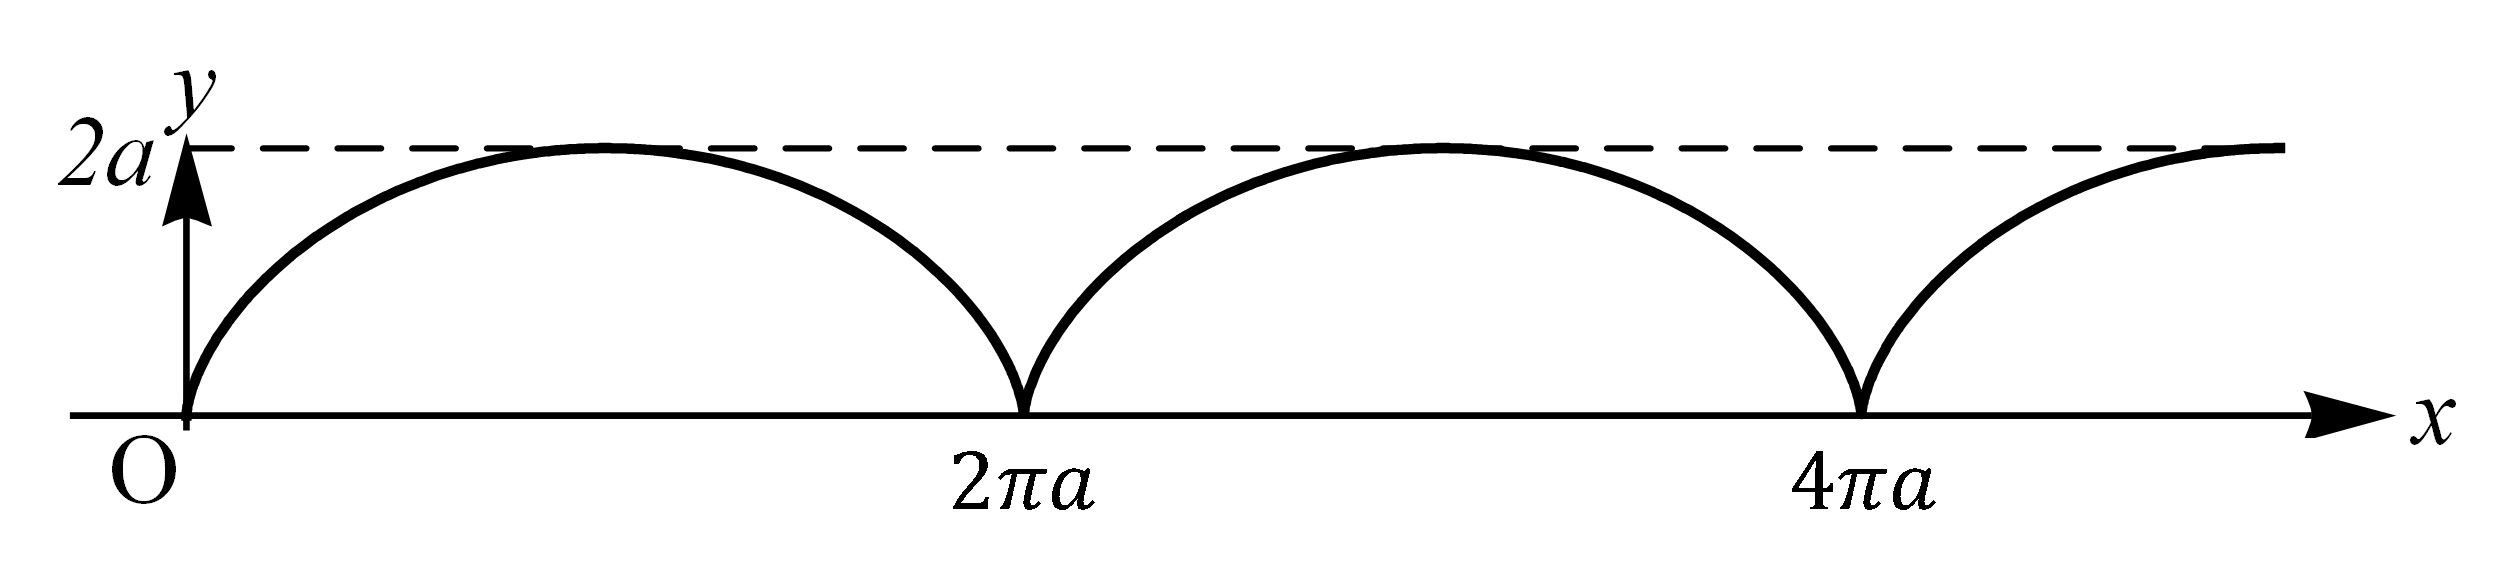
\includegraphics[height=0.1\textheight]{F:/life/2018AutumnTA/Exercises/11/Fig5-3-2.png}
\end{center}
\caption{习题7.5 3.(2)题图示}
\label{5-3-2}
\end{figure}
$x'(t)=a(1-\cos t),y'(t)=a\sin t$

$x''(t)=a\sin t,y''(t)=a\cos t$

$\therefore$曲率$k=\frac{|y''(t)x'(t)-y'(t)x''(t)|}{\{[x'(t)]^2+[y'(t)]^2\}^{\frac32}}=\frac{|a\cos t\cdot a(1-\cos t)-a\sin t\cdot a\sin t|}{\{[a(1-\cos t)]^2+[a\sin t]^2\}^{\frac32}}=\frac{|a^2\cos t-a^2|}{a^3(1-2\cos t+1)^{\frac32}}=\frac{|\cos t-1|}{a(2-2\cos t)^{\frac32}}\\
=\frac1{2\sqrt2a\sqrt{1-\cos t}}$

曲率半径$R=\frac1k=2\sqrt2a\sqrt{1-\cos t}$.

(3)由$\rho^2=2a^2\cos2\theta$得$\cos2\theta\geq0$,当$\theta$在$[0,2\pi)$内取值时,$0\leq2\theta\leq\frac\pi2\text{或}\frac32\pi\leq2\theta\leq\frac52\pi\text{或}\frac72\pi\leq2\theta<4\pi$,即$0\leq\theta\leq\frac\pi4\text{或}\frac34\pi\leq\theta\leq\frac54\pi\text{或}\frac74\pi\leq\theta<2\pi$,曲线形状如图~\ref{5-3-3}所示,
\begin{figure}[H]
\begin{center}
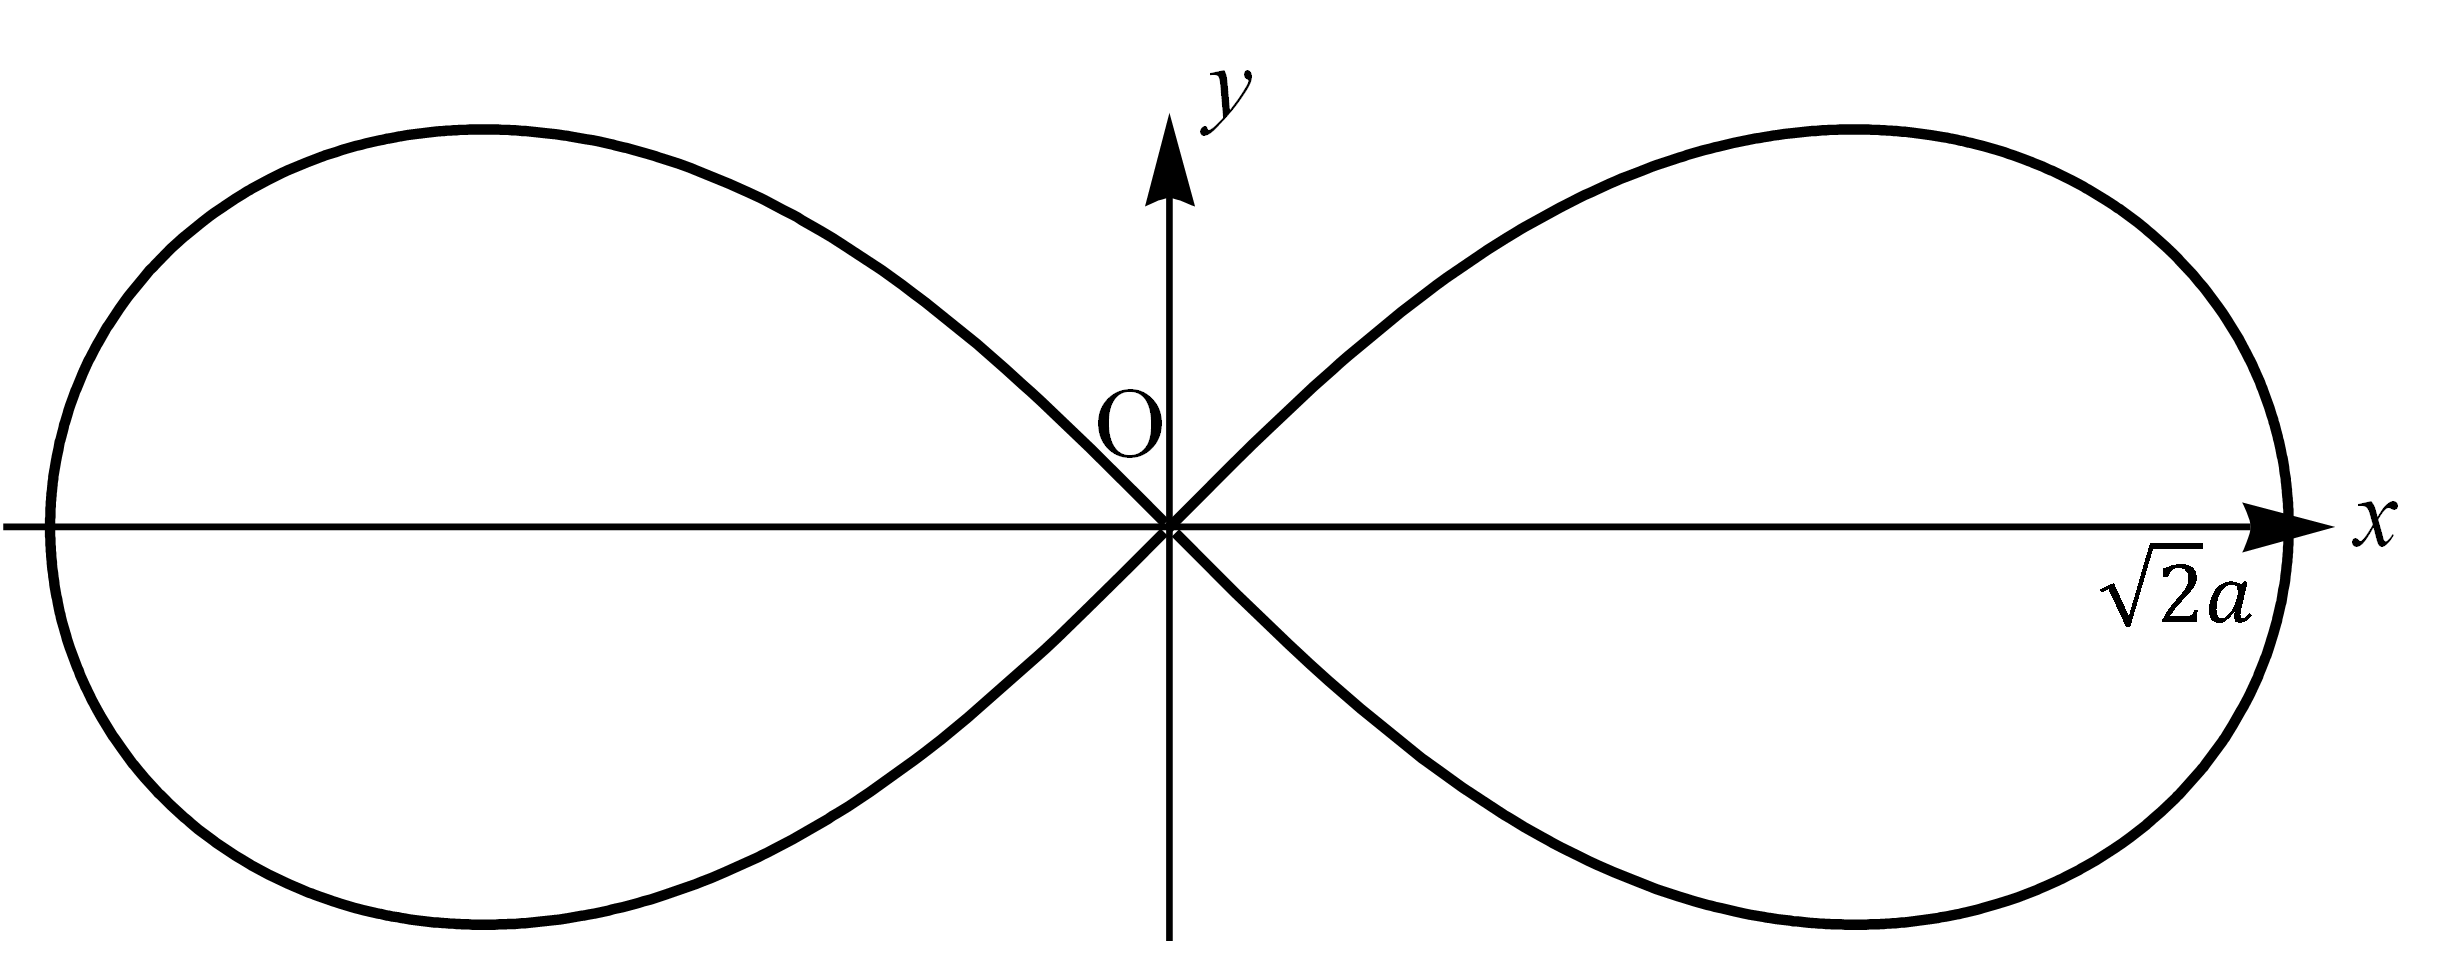
\includegraphics[height=0.2\textwidth]{F:/life/2018AutumnTA/Exercises/11/Fig5-3-3.png}
\end{center}
\caption{习题7.5 3.(3)题图示}
\label{5-3-3}
\end{figure}
将$\rho^2=2a^2\cos2\theta$两边对$\theta$求导得$2\rho\rho'=-4a^2\sin2\theta,\rho'=-\frac{2a^2\sin2\theta}\rho$

$\therefore\rho''=\frac{-4a^2\rho\cos2\theta+2a^2\rho'\sin2\theta}{\rho^2}=\frac{-4a^2\rho\cos2\theta-\frac{2a^2\sin2\theta}\rho2a^2\sin2\theta}{\rho^2}=-\frac{4a^2\rho^2\cos2\theta+4a^4\sin^22\theta}{\rho^3}\\
=-\frac{4a^22a^2\cos2\theta\cos2\theta+4a^4\sin^22\theta}{\rho^3}=-\frac{8a^4\cos^22\theta+4a^4\sin^22\theta}{\rho^3}=-\frac{4a^4\cos^22\theta+4a^4}{\rho^3}$

曲率$k=\frac{|\rho^2+2(\rho')^2-\rho\rho''|}{[\rho^2+(\rho')^2]^{\frac32}}=\frac{|\rho^2+2(-\frac{2a^2\sin2\theta}\rho)^2+\frac{4a^4\cos^22\theta+4a^4}{\rho^3}\rho|}{[\rho^2+(-\frac{2a^2\sin2\theta}\rho)^2]^{\frac32}}=\frac{|\rho^5+8a^4\rho\sin^22\theta+(4a^4\cos^22\theta+4a^4)\rho|}{(\rho^4+4a^4\sin^22\theta)^{\frac32}}\\
=\frac{|\rho^5+8a^4\rho+(-4a^4\cos^22\theta+4a^4)\rho|}{(\rho^4+4a^4-4a^4\cos^22\theta)^{\frac32}}=\frac{|\rho^5+8a^4\rho+(-\rho^4+4a^4)\rho|}{(4a^4)^{\frac32}}=\frac{12a^4\rho}{8a^6}=\frac{3\rho}{2a^2}=\frac{3\sqrt2a\sqrt{\cos2\theta}}{2a^2}=\frac3a\sqrt{\frac{\cos2\theta}2}$.

曲率半径$R=\frac1k=\frac a3\sqrt{\frac2{\cos2\theta}}$.

\item求曲线$y=\mathrm e^x$上弯曲程度最大的点.

解:$y'=\mathrm e^x,y''=\mathrm e^x$

曲率$k=\frac{|y''|}{[1+(y')^2]^{\frac32}}=\frac{\mathrm e^x}{(1+\mathrm e^{2x})^{\frac32}}$

$k'=\frac{\mathrm e^x(1+\mathrm e^{2x})^{\frac32}-\mathrm e^x\frac32(1+\mathrm e^{2x})^{\frac12}2\mathrm e^{2x}}{(1+\mathrm e^{2x})^3}=\frac{\mathrm e^x(1+\mathrm e^{2x})-3\mathrm e^x\mathrm e^{2x}}{(1+\mathrm e^{2x})^{\frac52}}=\frac{\mathrm e^x-2\mathrm e^{3x}}{(1+\mathrm e^{2x})^{\frac52}}=\frac{\mathrm e^x(1-2\mathrm e^{2x})}{(1+\mathrm e^{2x})^{\frac52}}$

当$x=\ln\frac{\sqrt2}2$时,$k'=0$,当$x<\ln\frac{\sqrt2}2$时,$k'>0$,当$x>\ln\frac{\sqrt2}2$时,$k'<0$

$\therefore k(x)$在区间$(-\infty,+\infty)$上处处可导且$x=\ln\frac{\sqrt2}2$是$k(x)$在$(-\infty,+\infty)$上的唯一驻点,且是极大值点,故是最大值点,即曲线$y=\mathrm e^x$上弯曲程度最大的点为$(\ln\frac{\sqrt2}2,\frac{\sqrt2}2)$.

\item求下列曲面所围空间图形的体积:
\newline
(1)椭球面$\frac{x^2}{a^2}+\frac{y^2}{b^2}+\frac{z^2}{c^2}=1$;
\newline
(2)$x^2+y^2+z^2=R^2$与$x^2+y^2=\frac{R^2}4$.

解:(1)椭球面的图形如图~\ref{5-5-1-1}所示,
\begin{figure}[H]
\begin{center}
    \subfloat[]{\label{5-5-1-1} {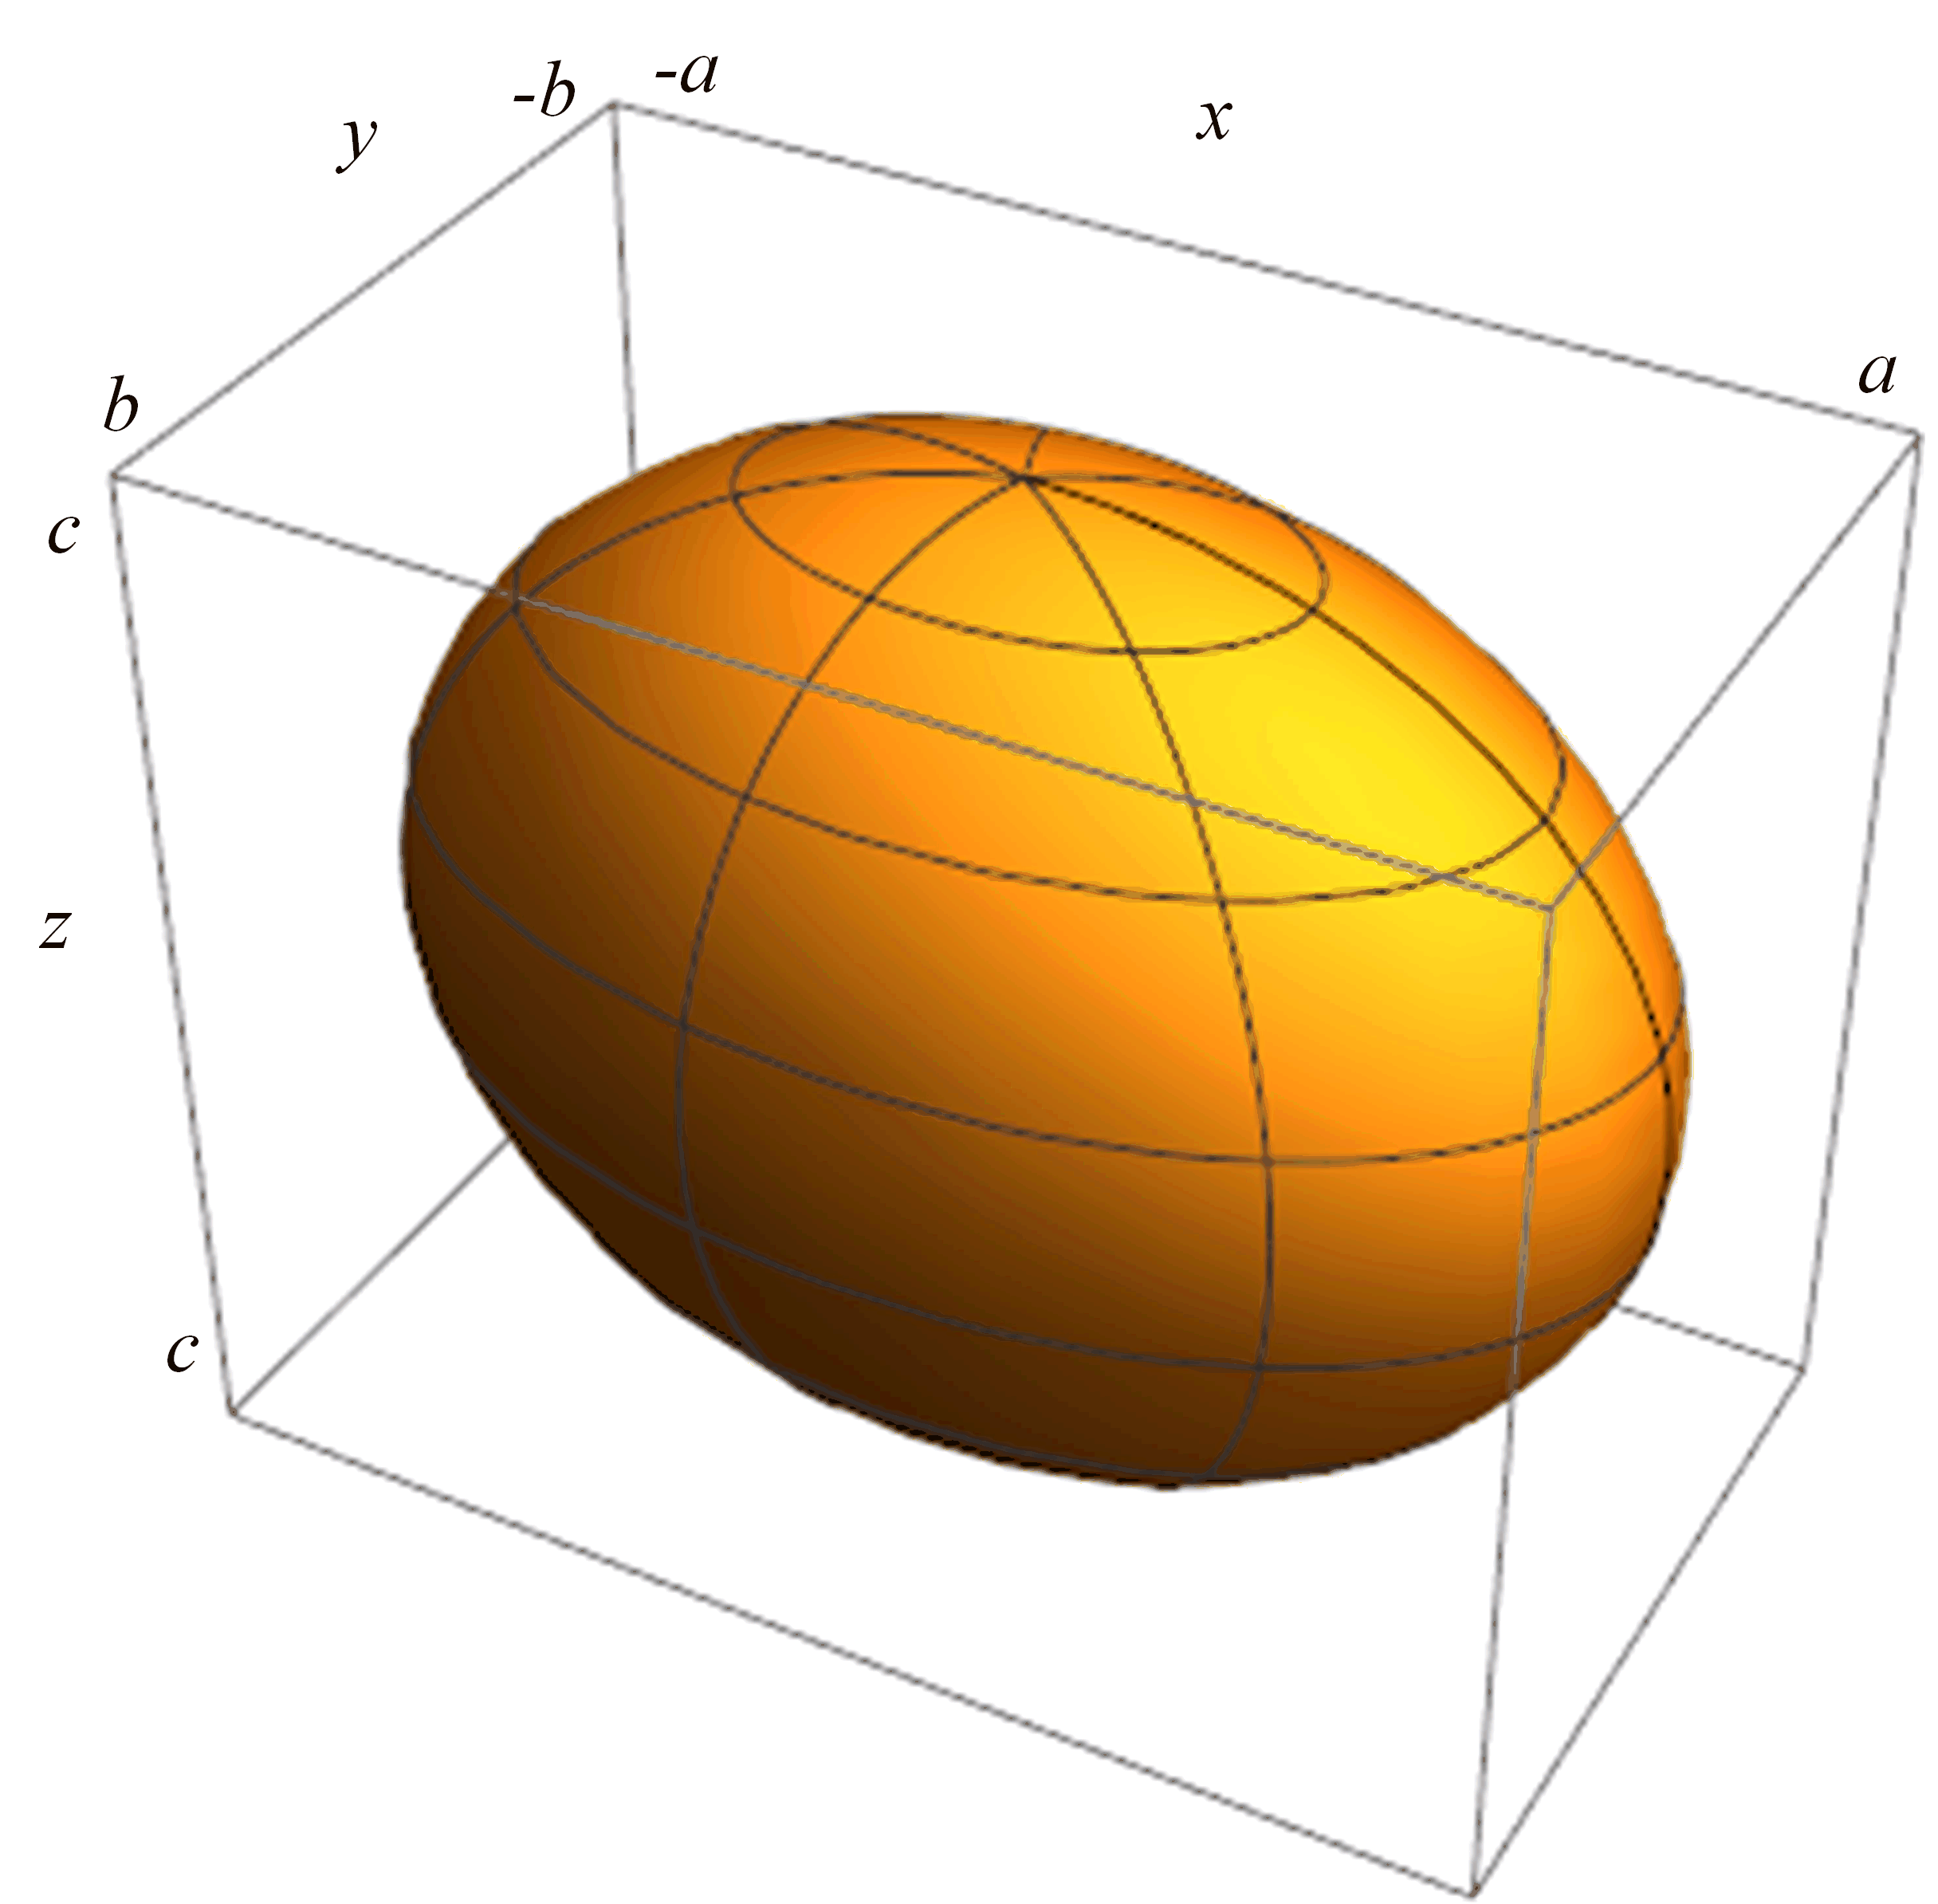
\includegraphics[height=0.3\textheight]{F:/life/2018AutumnTA/Exercises/11/Fig5-5-1-1.png} }}
    \subfloat[]{\label{5-5-1-2} {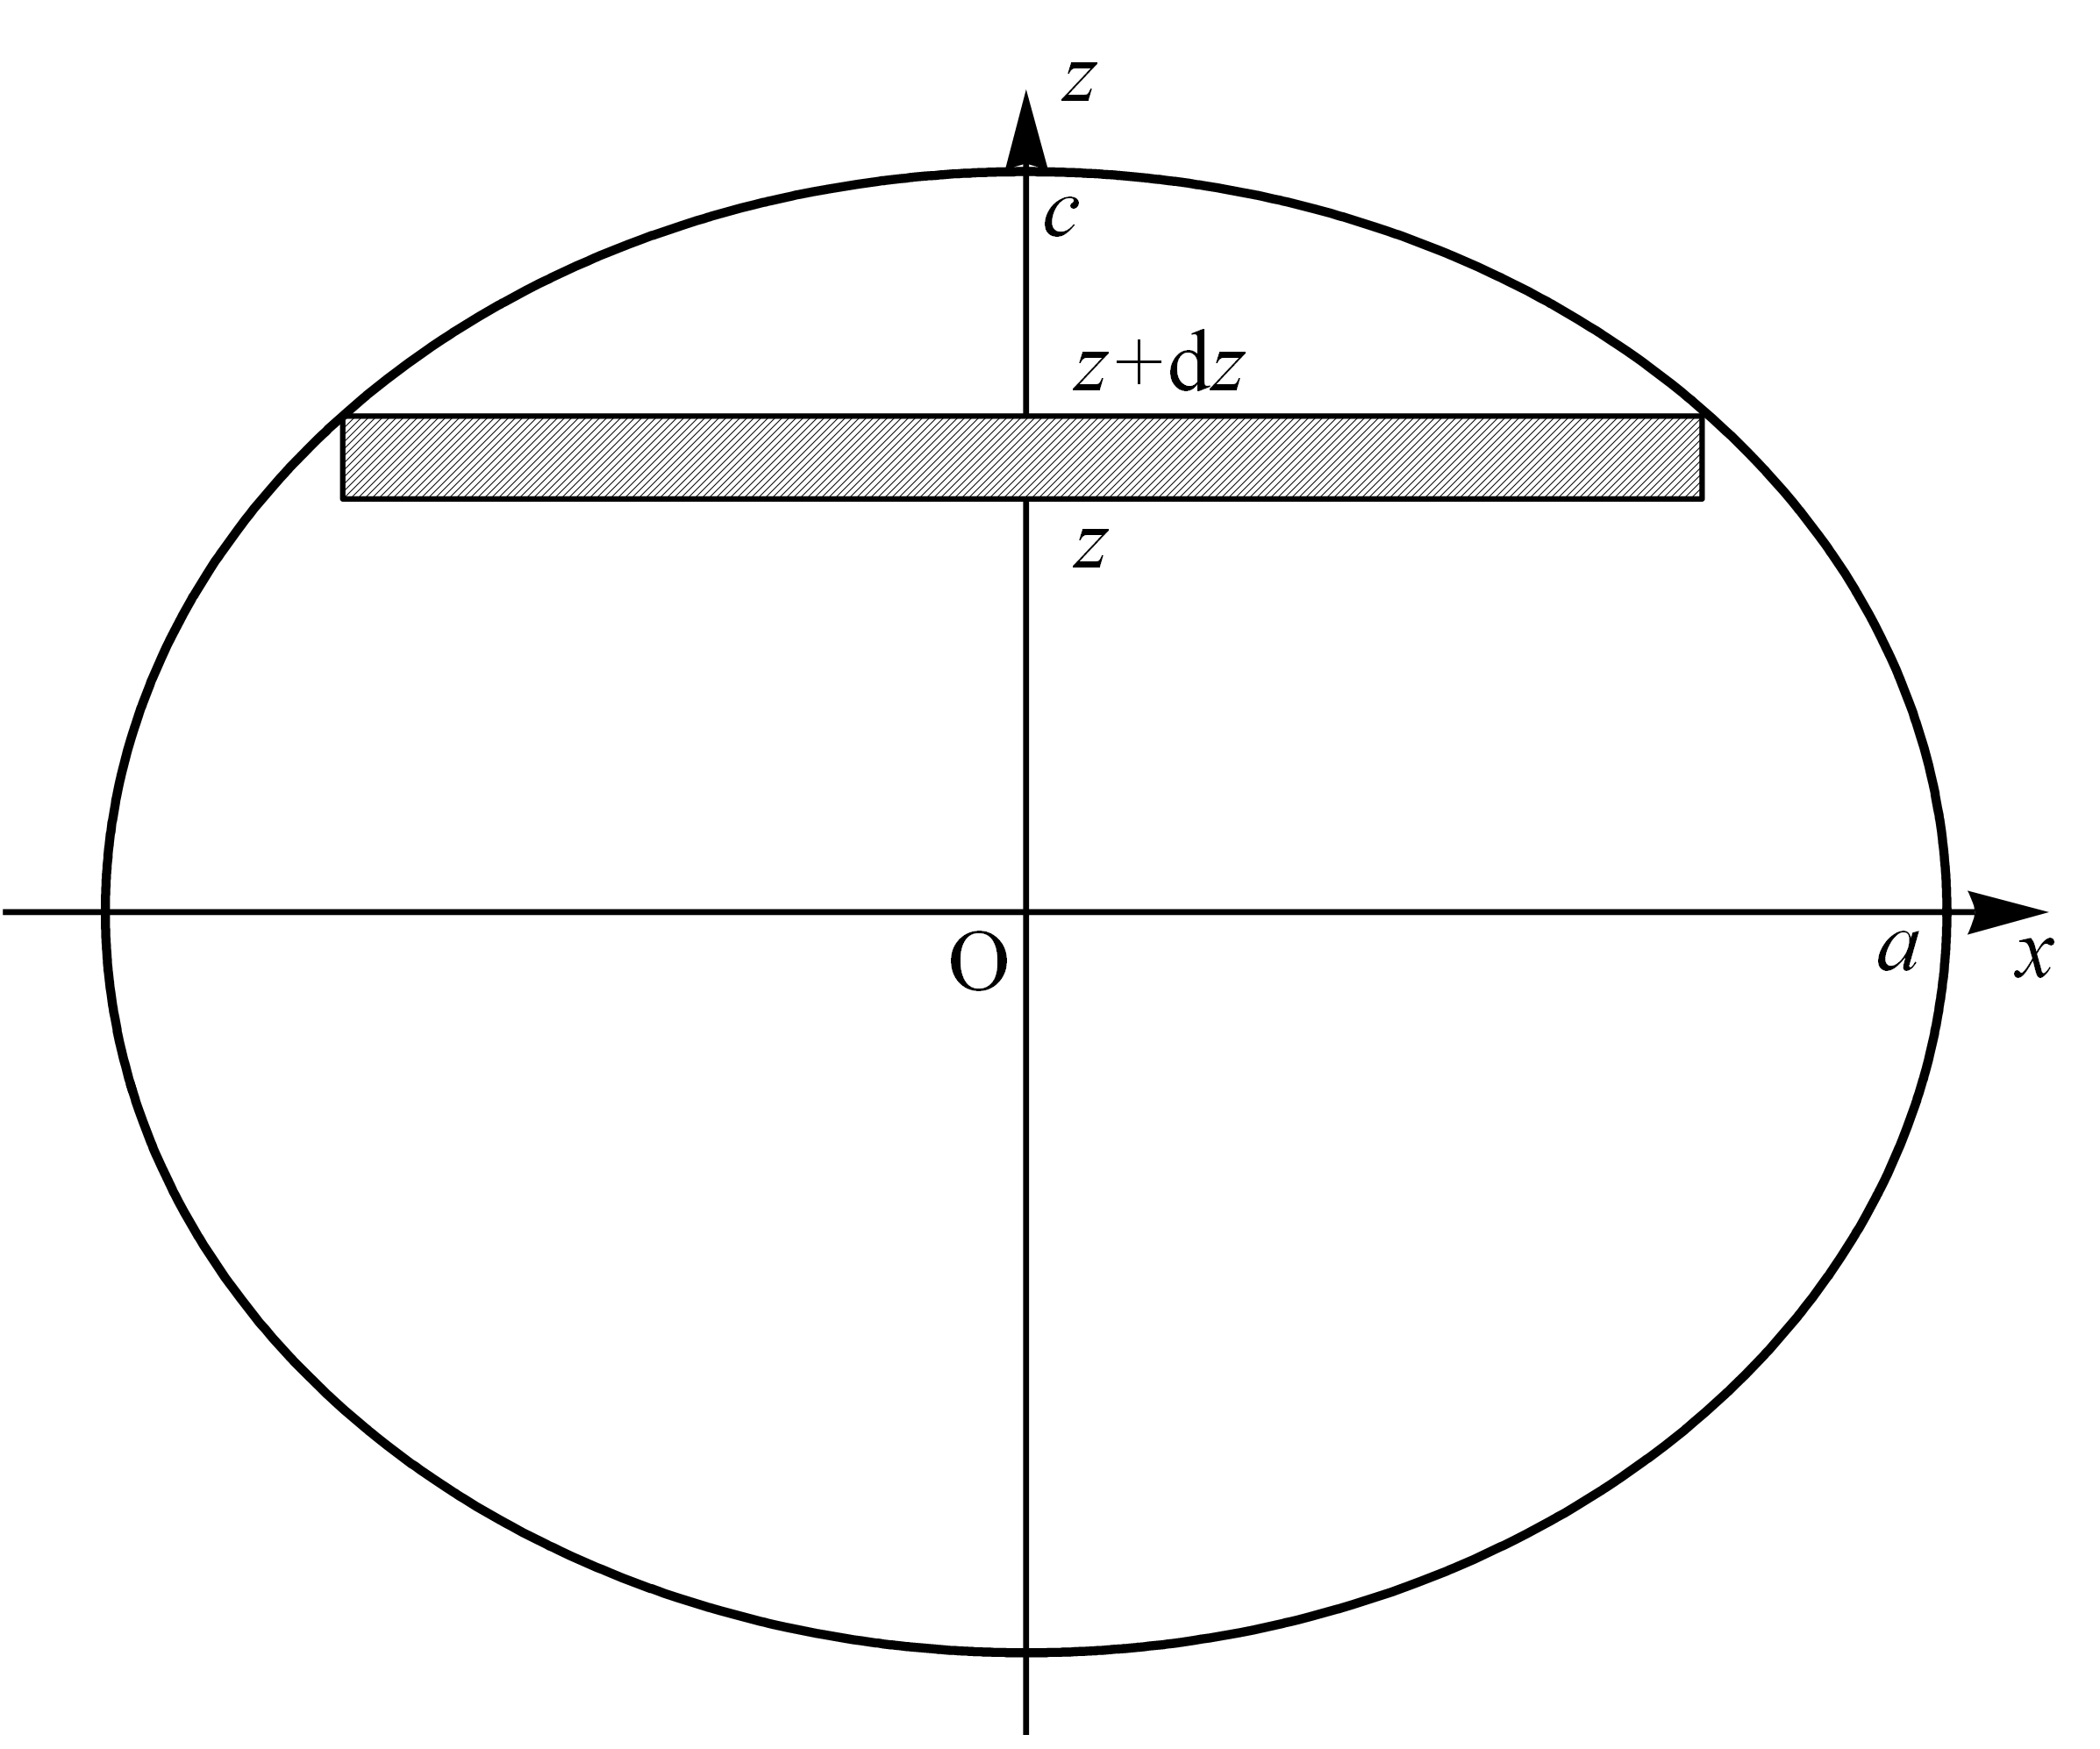
\includegraphics[height=0.3\textheight]{F:/life/2018AutumnTA/Exercises/11/Fig5-5-1-2.png} }}
\end{center}
\caption{习题7.5 5.(1)题图示}
\label{5-5-1}
\end{figure}
竖坐标为$z$时取图~\ref{5-5-1-2}所示的体积元,截面方程为$\frac{x^2}{a^2(1-\frac{z^2}{c^2})}+\frac{y^2}{b^2(1-\frac{z^2}{c^2})}=1$

截面面积$S=\pi a\sqrt{1-\frac{z^2}{c^2}}b\sqrt{1-\frac{z^2}{c^2}}=\pi ab(1-\frac{z^2}{c^2})$

该椭球的体积$V=\int_{-c}^c\pi ab(1-\frac{z^2}{c^2})\mathrm dz=\pi ab(z-\frac1{3c^2}z^3)\Big|_{-c}^c=\frac43\pi abc$.

(2)球面$x^2+y^2+z^2=R^2$和圆柱面$x^2+y^2=\frac{R^2}4$的图形如图~\ref{5-5-2-1}所示,二者所围空间如图~\ref{5-5-2-2}所示,
\begin{figure}[H]
\begin{center}
	\subfloat[]{\label{5-5-2-1}
{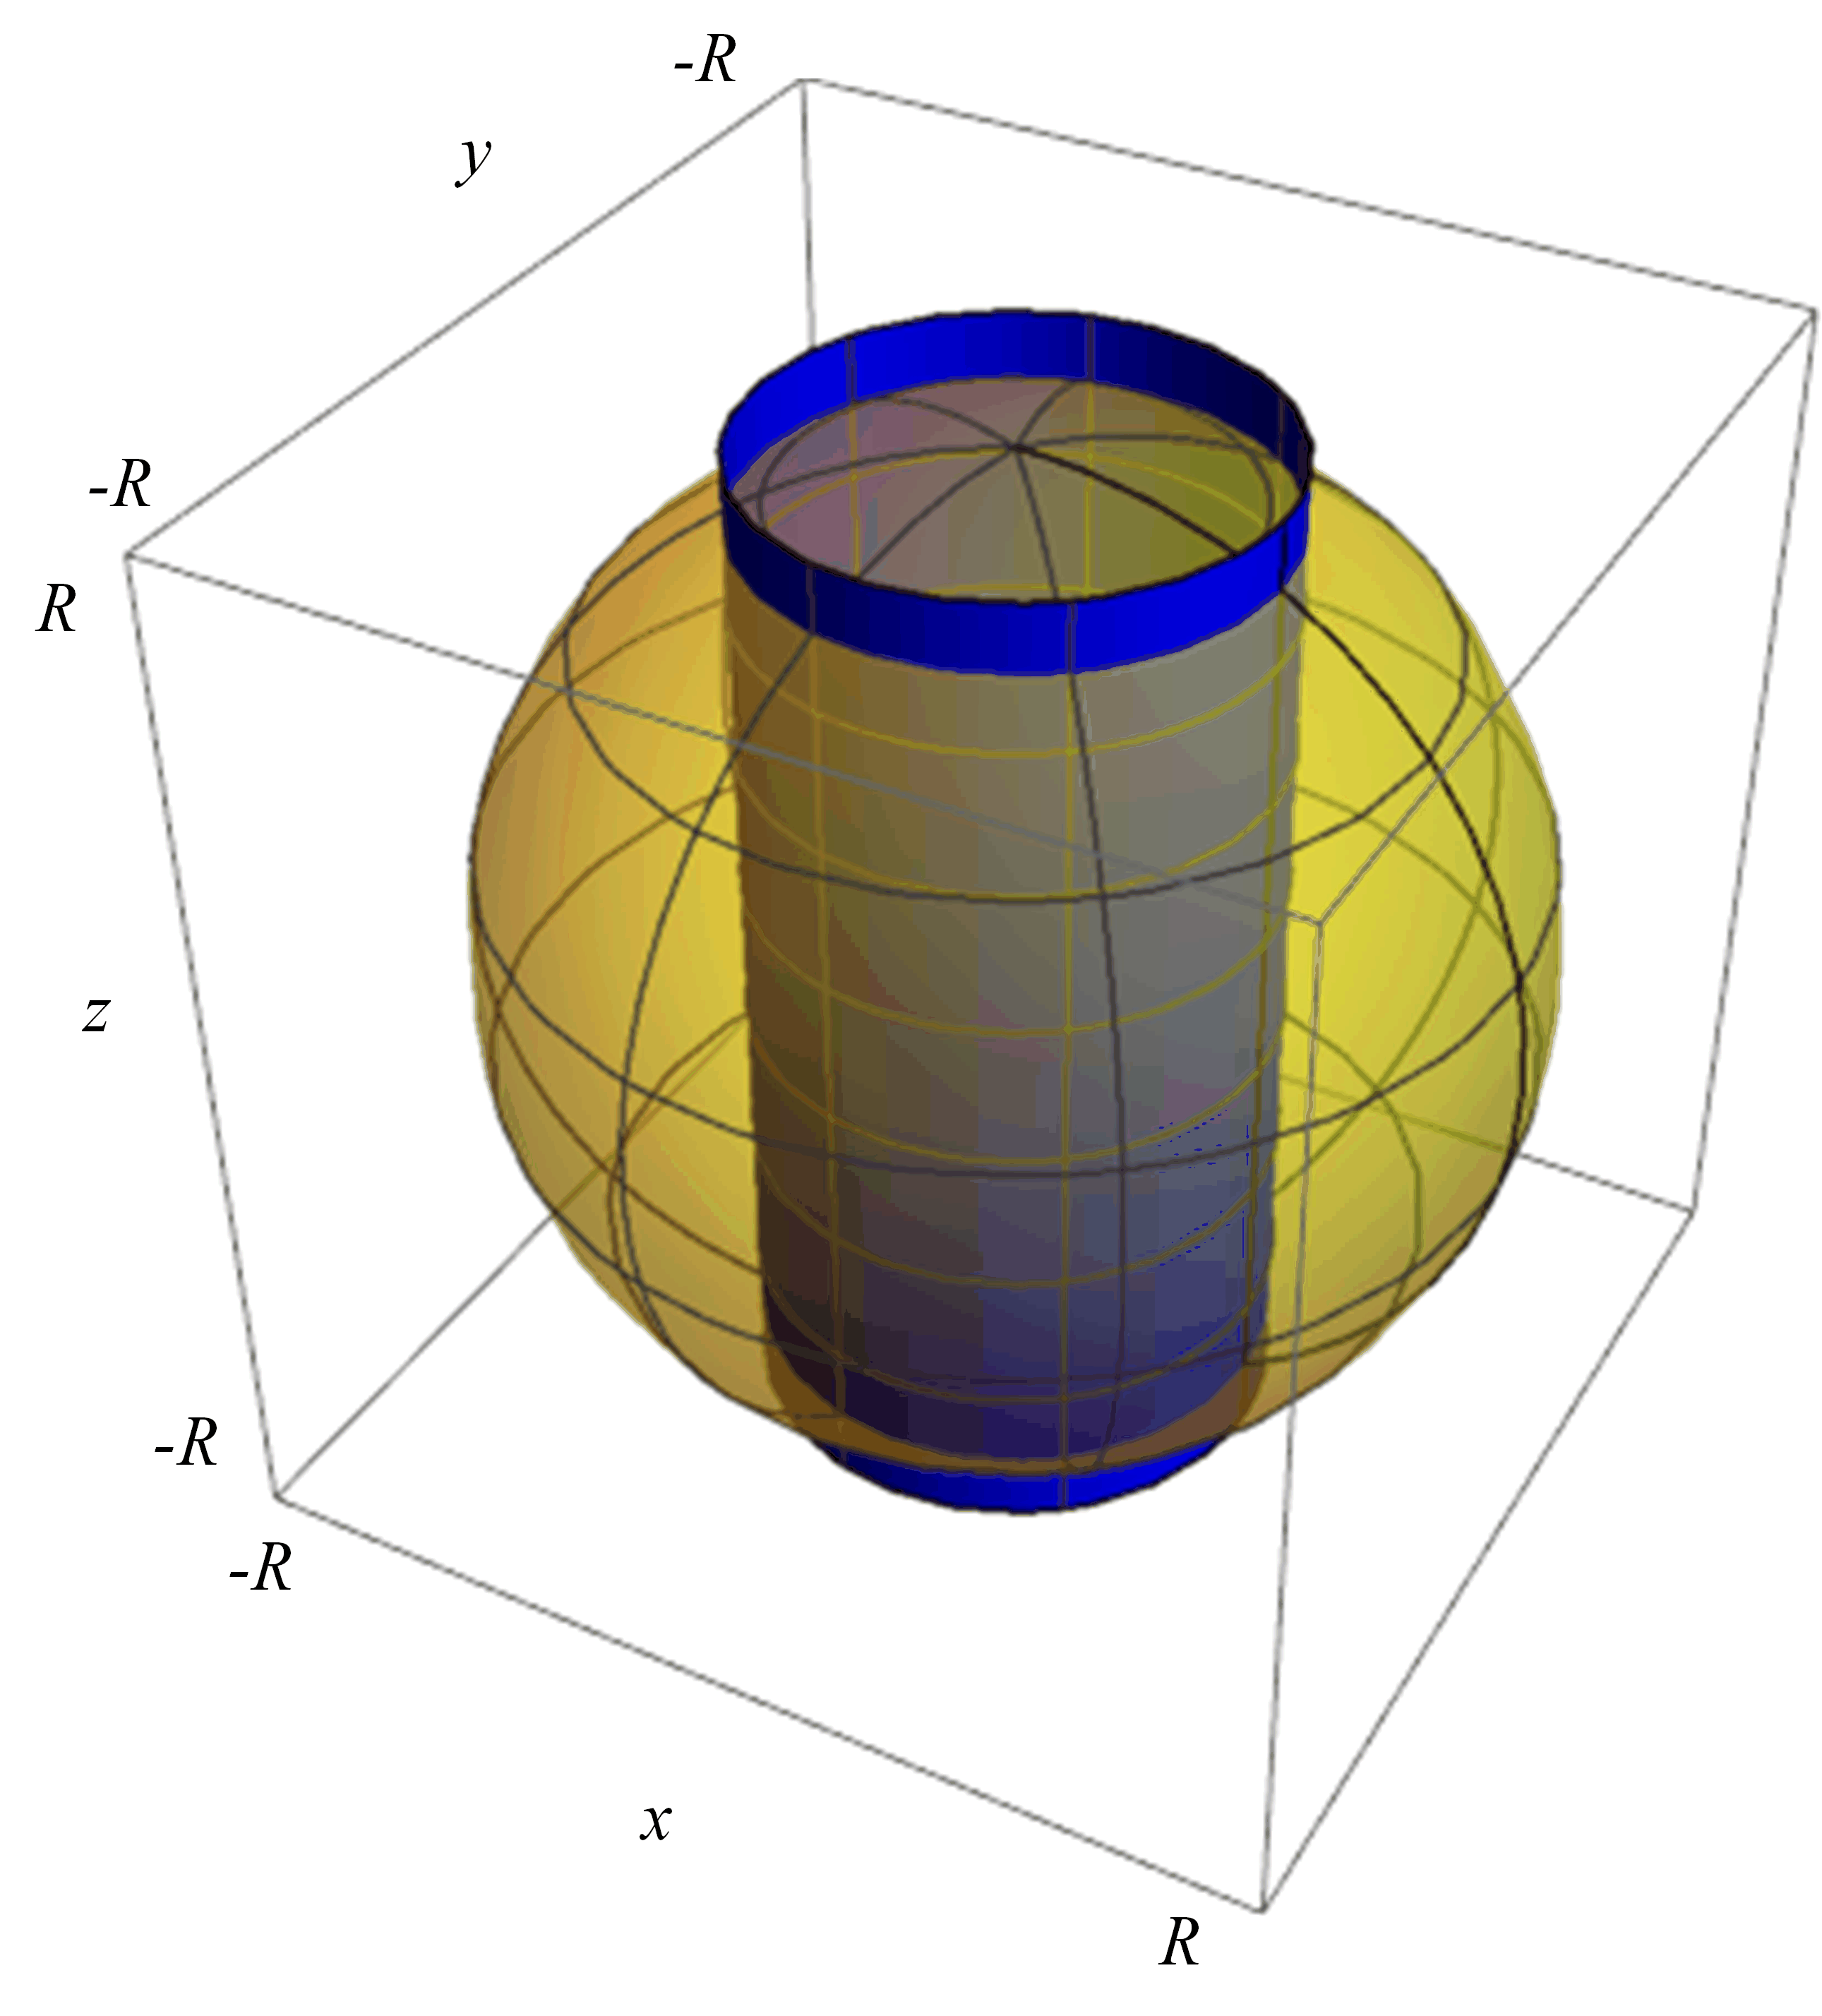
\includegraphics[height=0.4\textheight]{F:/life/2018AutumnTA/Exercises/11/Fig5-5-2-1.png} }}
    \subfloat[]{\label{5-5-2-2} {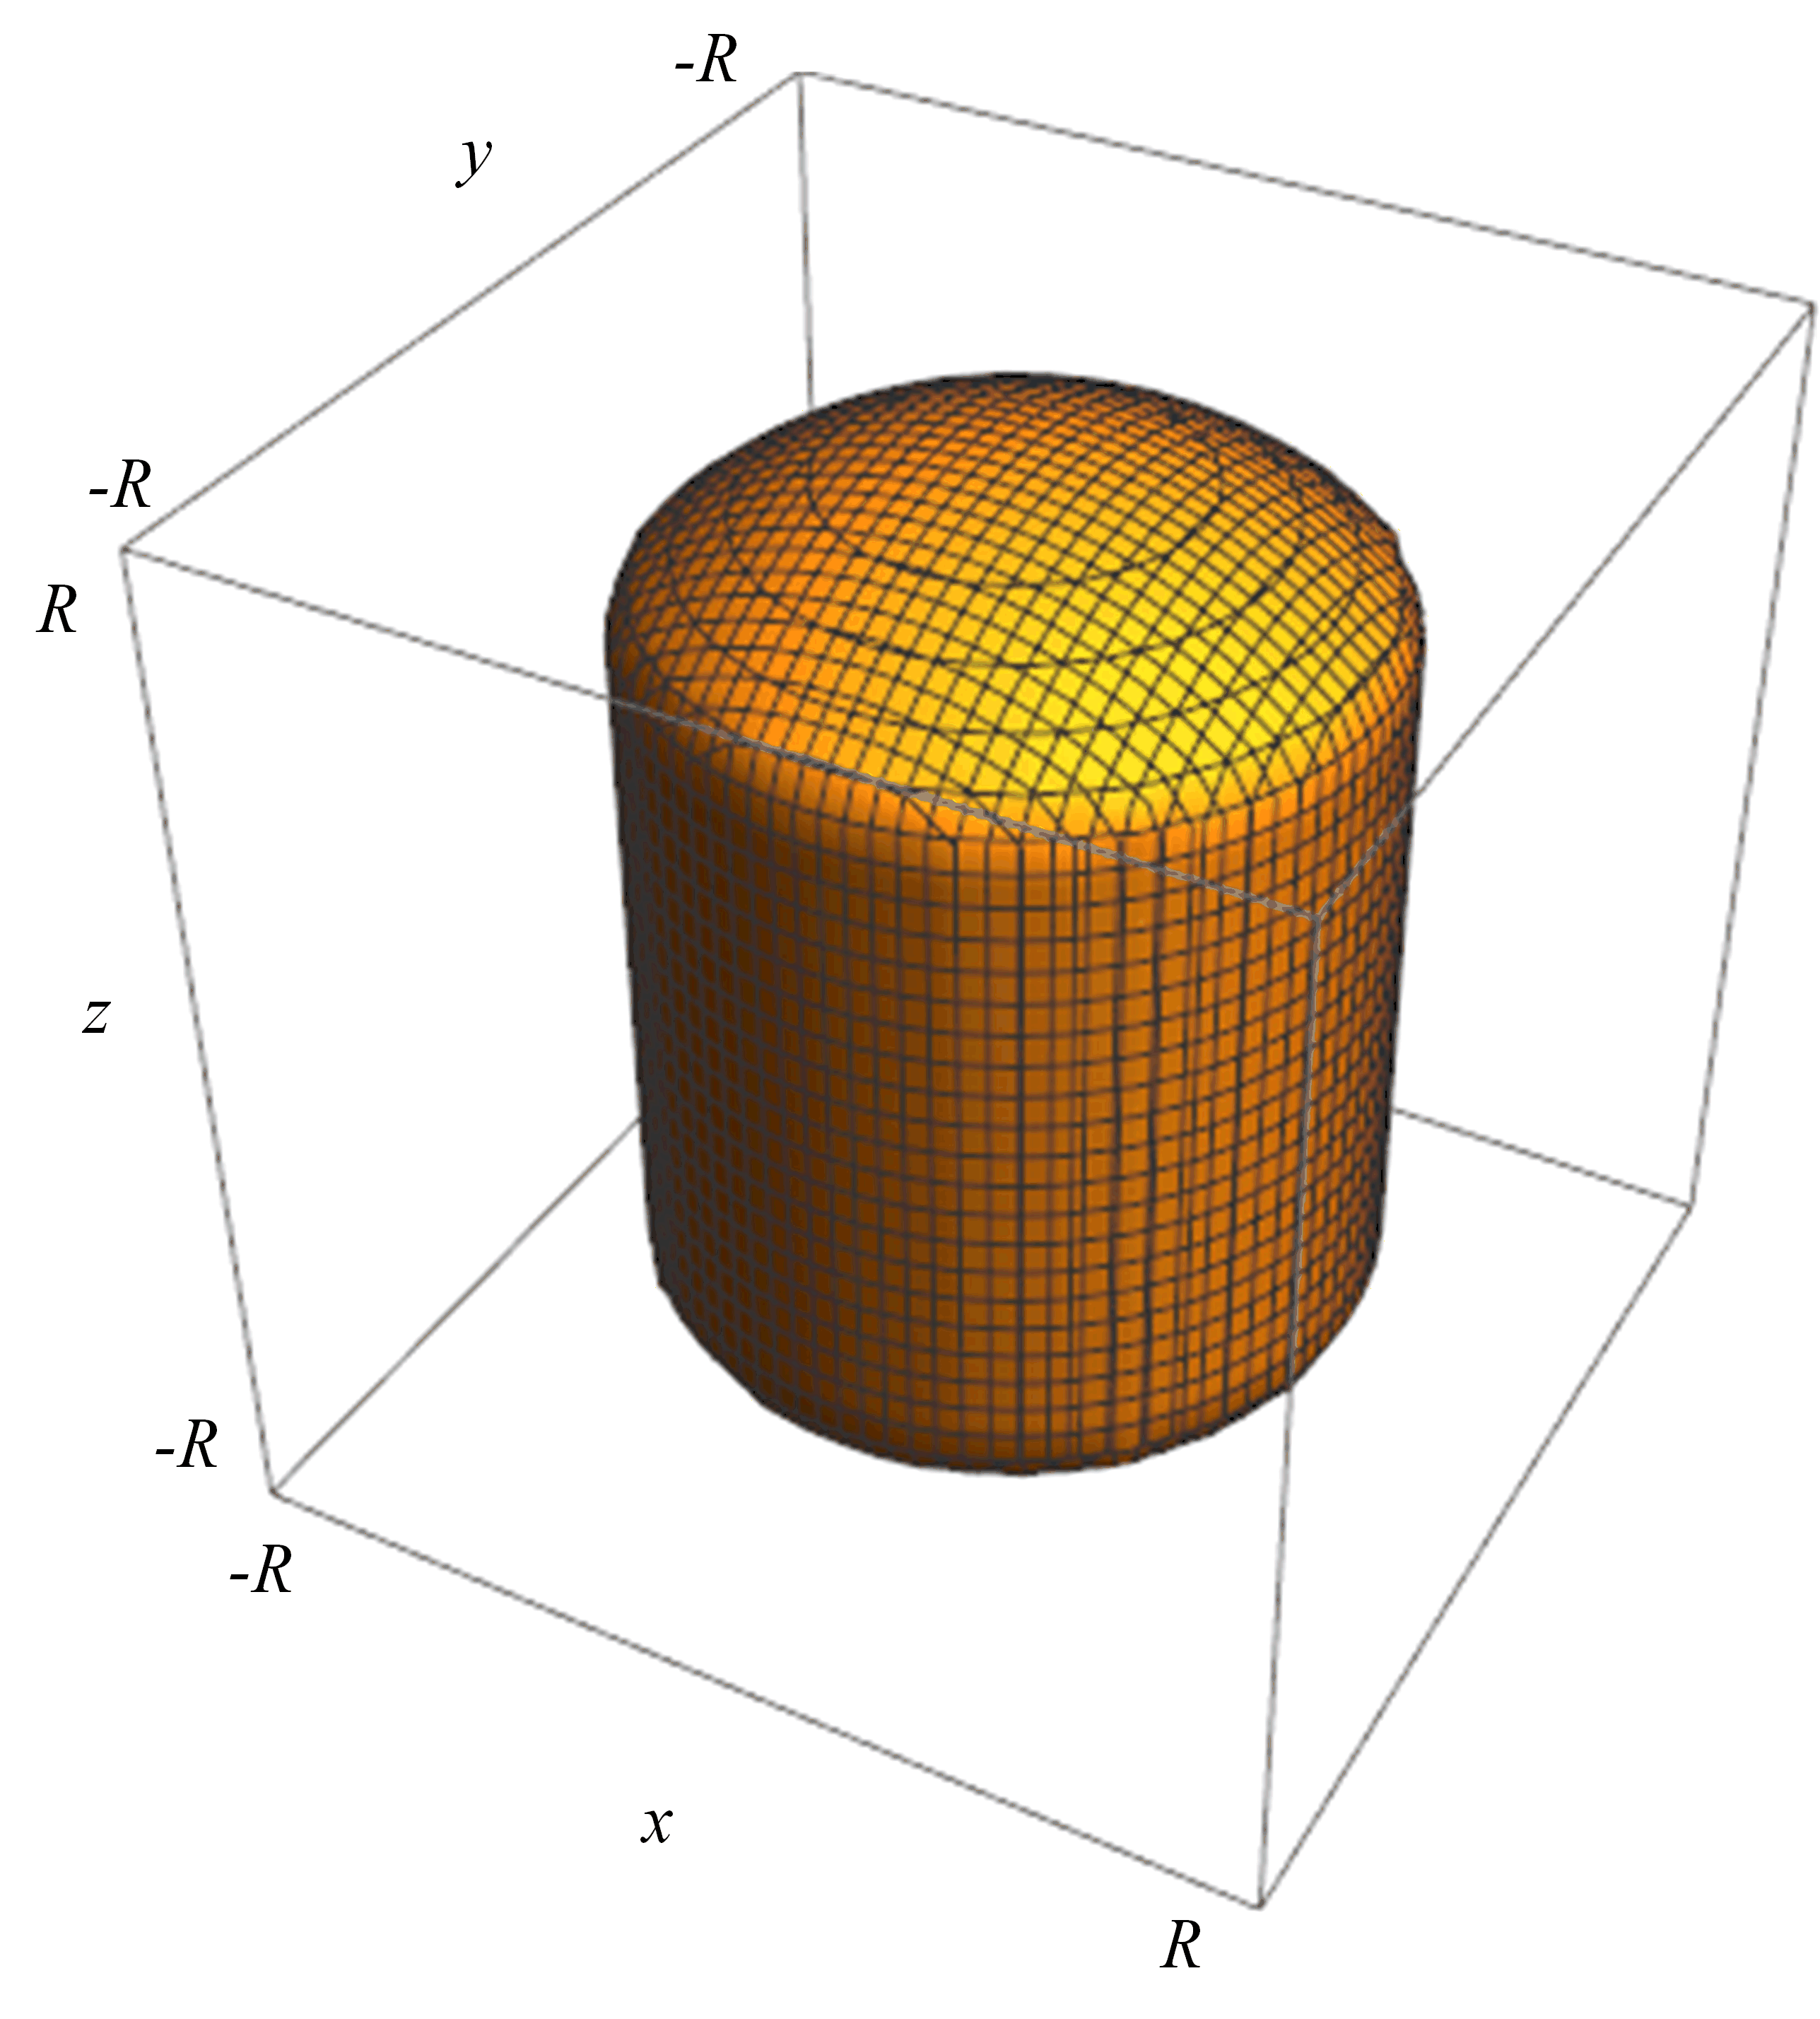
\includegraphics[height=0.4\textheight]{F:/life/2018AutumnTA/Exercises/11/Fig5-5-2-2.png} }}\\
    \subfloat[]{\label{5-5-2-3} {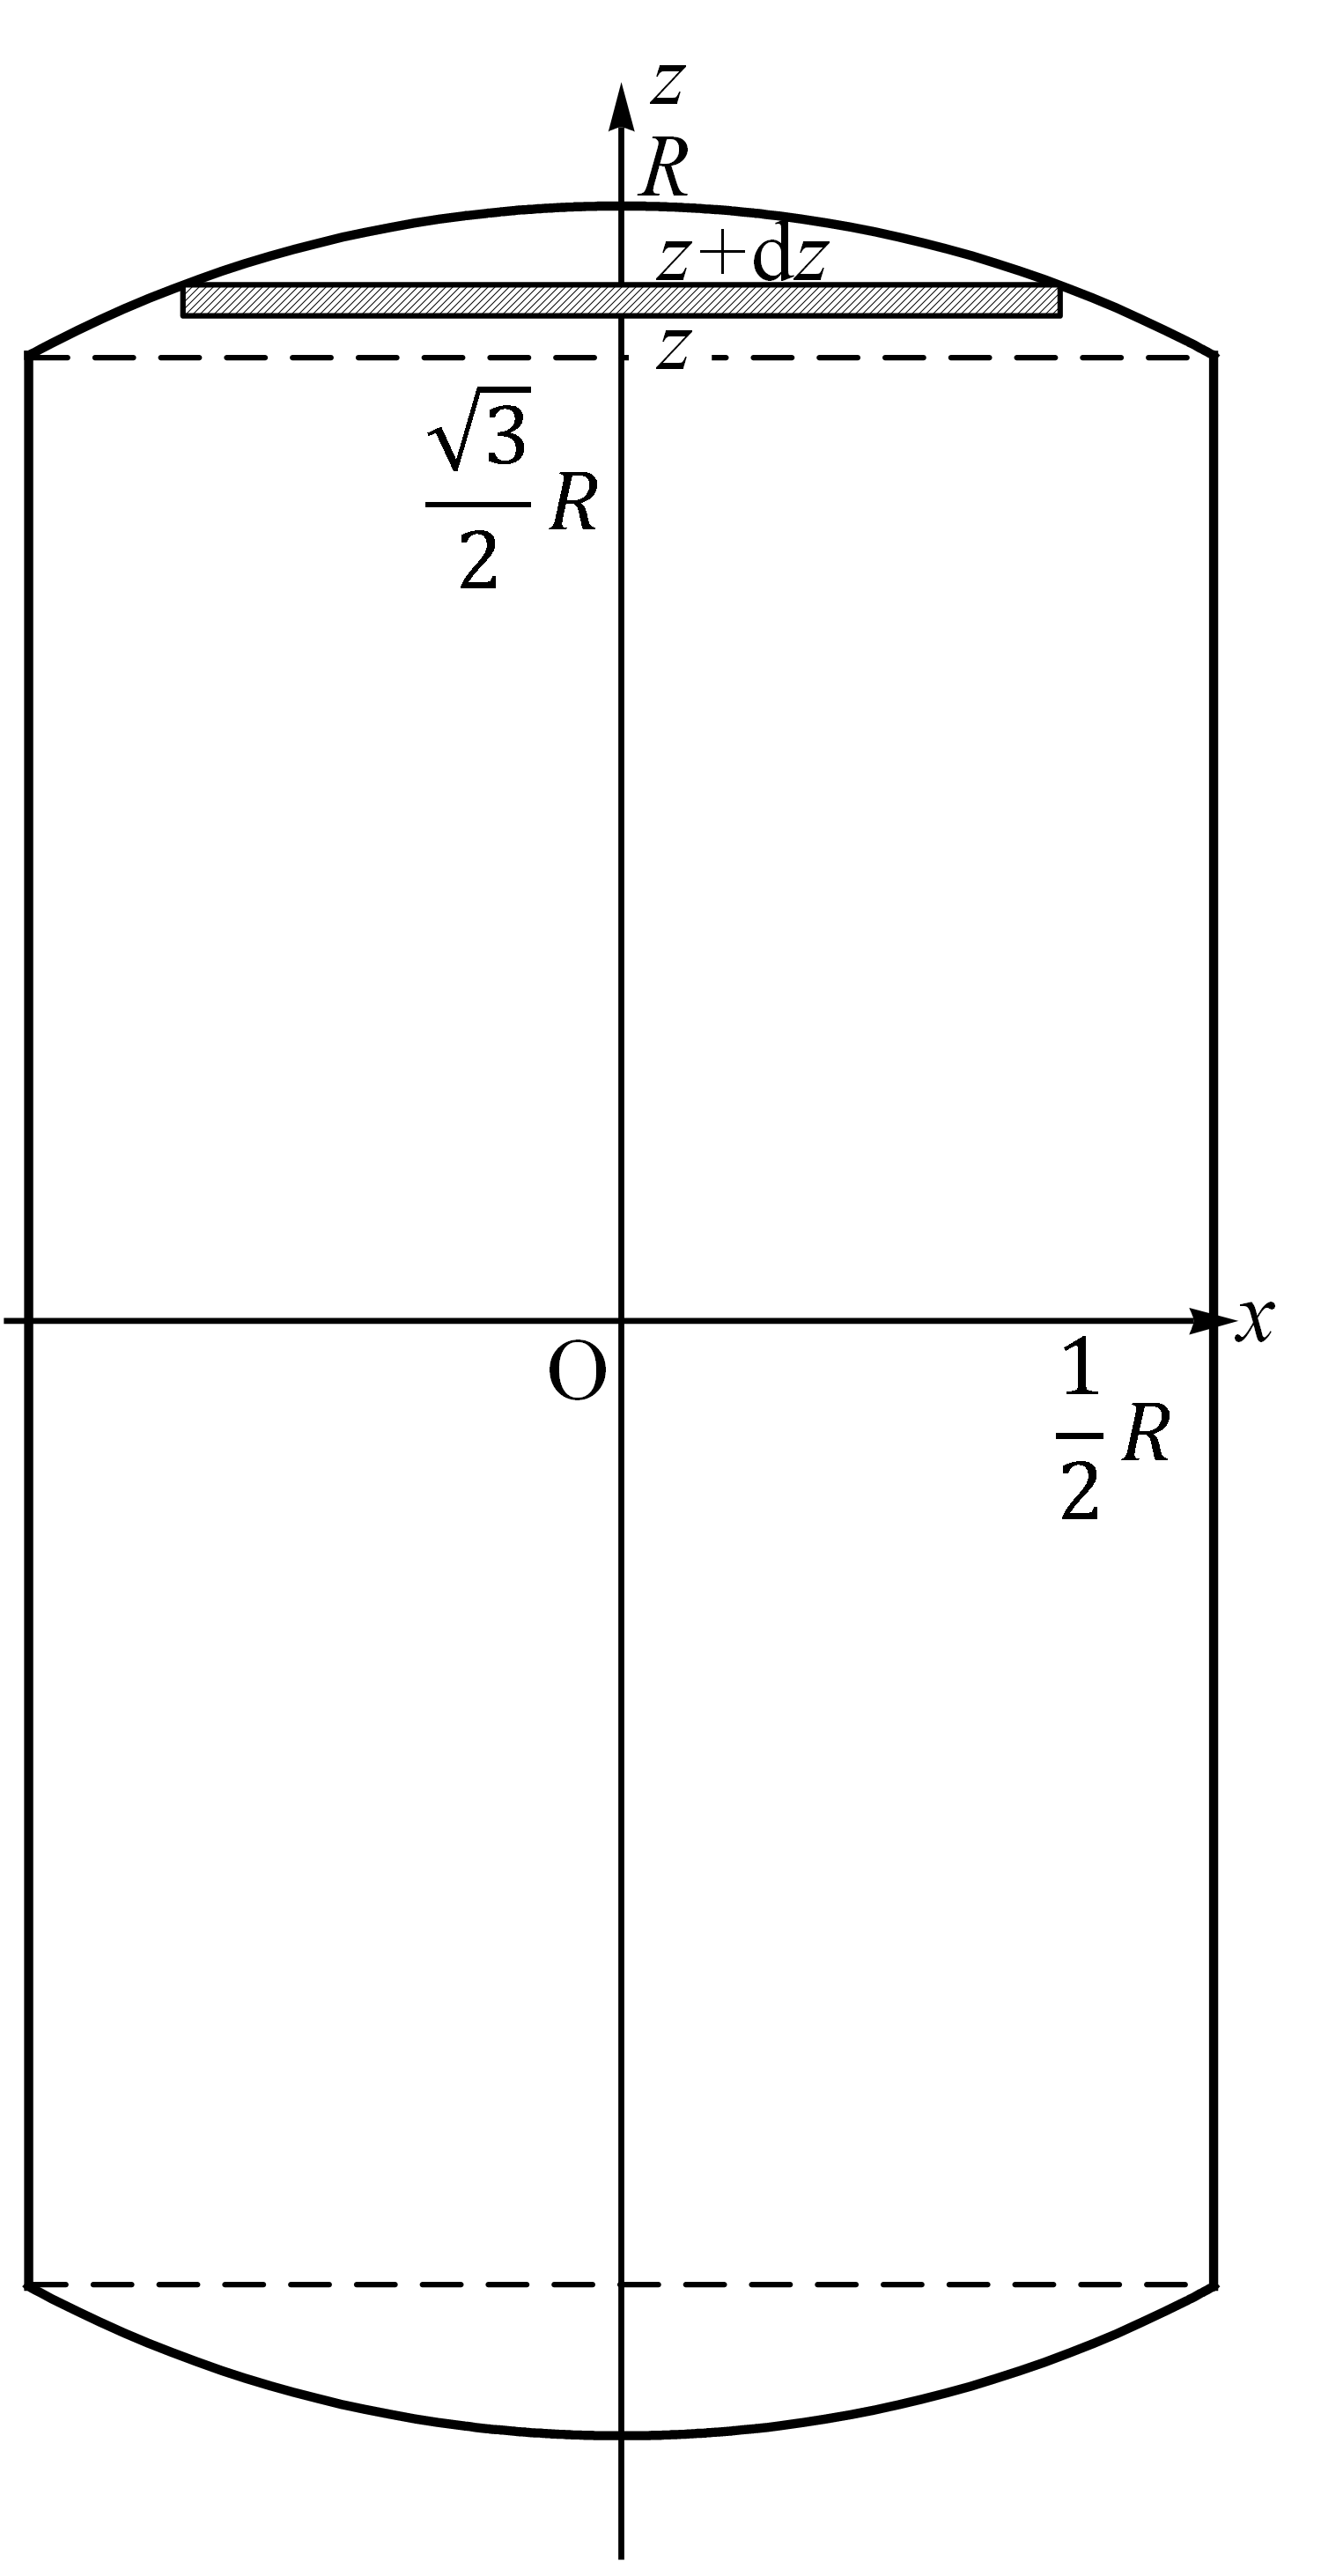
\includegraphics[height=0.4\textheight]{F:/life/2018AutumnTA/Exercises/11/Fig5-5-2-3.png} }}
\end{center}
\caption{习题7.5 5.(2)题图示}
\label{5-5-2}
\end{figure}
由$\begin{cases}
x^2+y^2+z^2=R^2\\
x^2+y^2=\frac{R^2}4
\end{cases}$得$z=\pm\frac{\sqrt3}2R$,故该空间图形可视为高为$\sqrt3R$,半径为$\frac12R$的圆柱和两个半径为$R$,高为$R-\frac{\sqrt3}2R$的球缺组成的组合体

圆柱的体积为$V_1=\pi(\frac12R)^2\cdot\sqrt3R=\frac{\sqrt3}4\pi R^3$

对于球缺,当竖坐标为$z$时取图~\ref{5-5-2-3}所示的体积元,球缺的体积为$V_2=2\int_{\frac{\sqrt3}2R}^R\pi(R^2-z^2)\mathrm dz=2\pi (R^2z-\frac13z^3)\Big|_{\frac{\sqrt3}2R}^R=\frac43\pi R^3-\frac{3\sqrt3}4\pi R^3$

该组合体的体积为$V=V_1+V_2=(\frac43-\frac{\sqrt3}2)\pi R^3$.
\item求下列旋转体的体积:
\newline
(1)$y=\sin x(0\leq x\leq\pi)$绕$x$轴旋转;
\newline
(2)$\begin{cases}
x=a\cos^3t,\\
y=a\sin^3t,
\end{cases}0\leq t\leq2\pi$绕$y$轴,$a>0$;
\newline
(3)$\rho=a(1+\cos\theta)$绕极轴,$a>0$.

解:(1)旋转体如图~\ref{5-6-1-1}所示,取如图~\ref{5-6-1-2}所示的体积元,
\begin{figure}[H]
\begin{center}
 \subfloat[]{\label{5-6-1-1}
{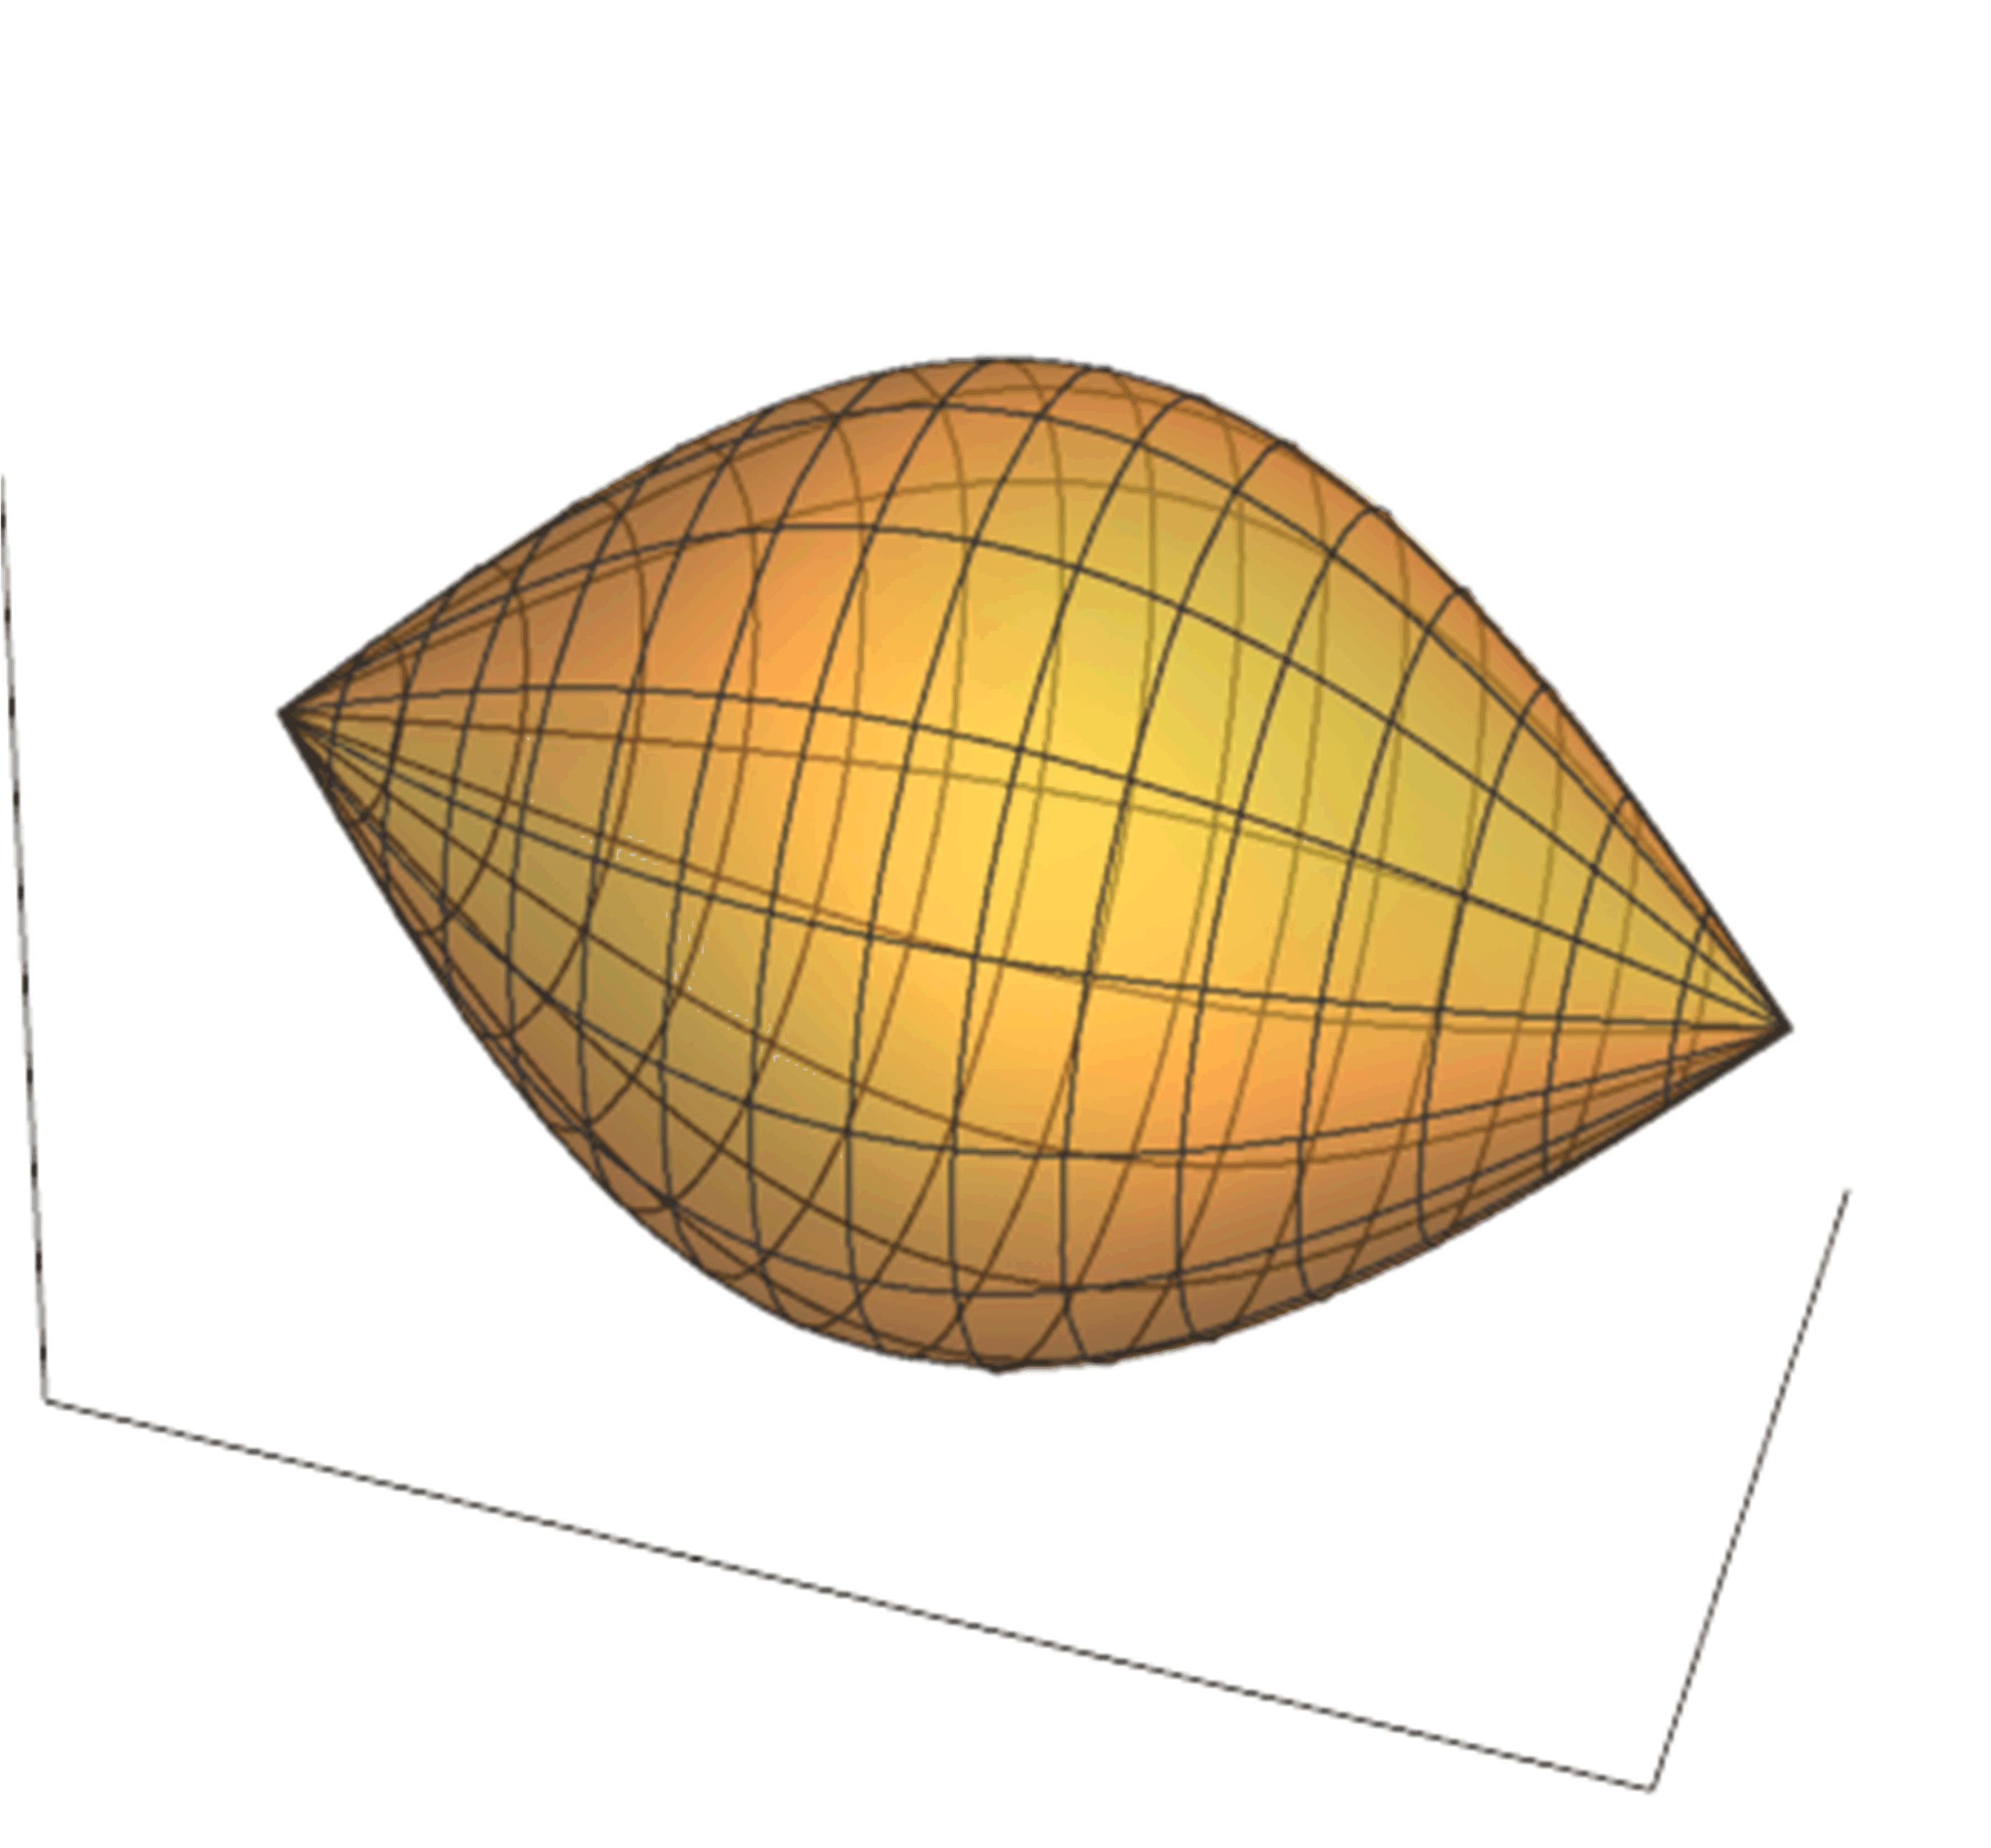
\includegraphics[height=0.3\textheight]{F:/life/2018AutumnTA/Exercises/11/Fig5-6-1-2.png} }}
	\subfloat[]{\label{5-6-1-2}
{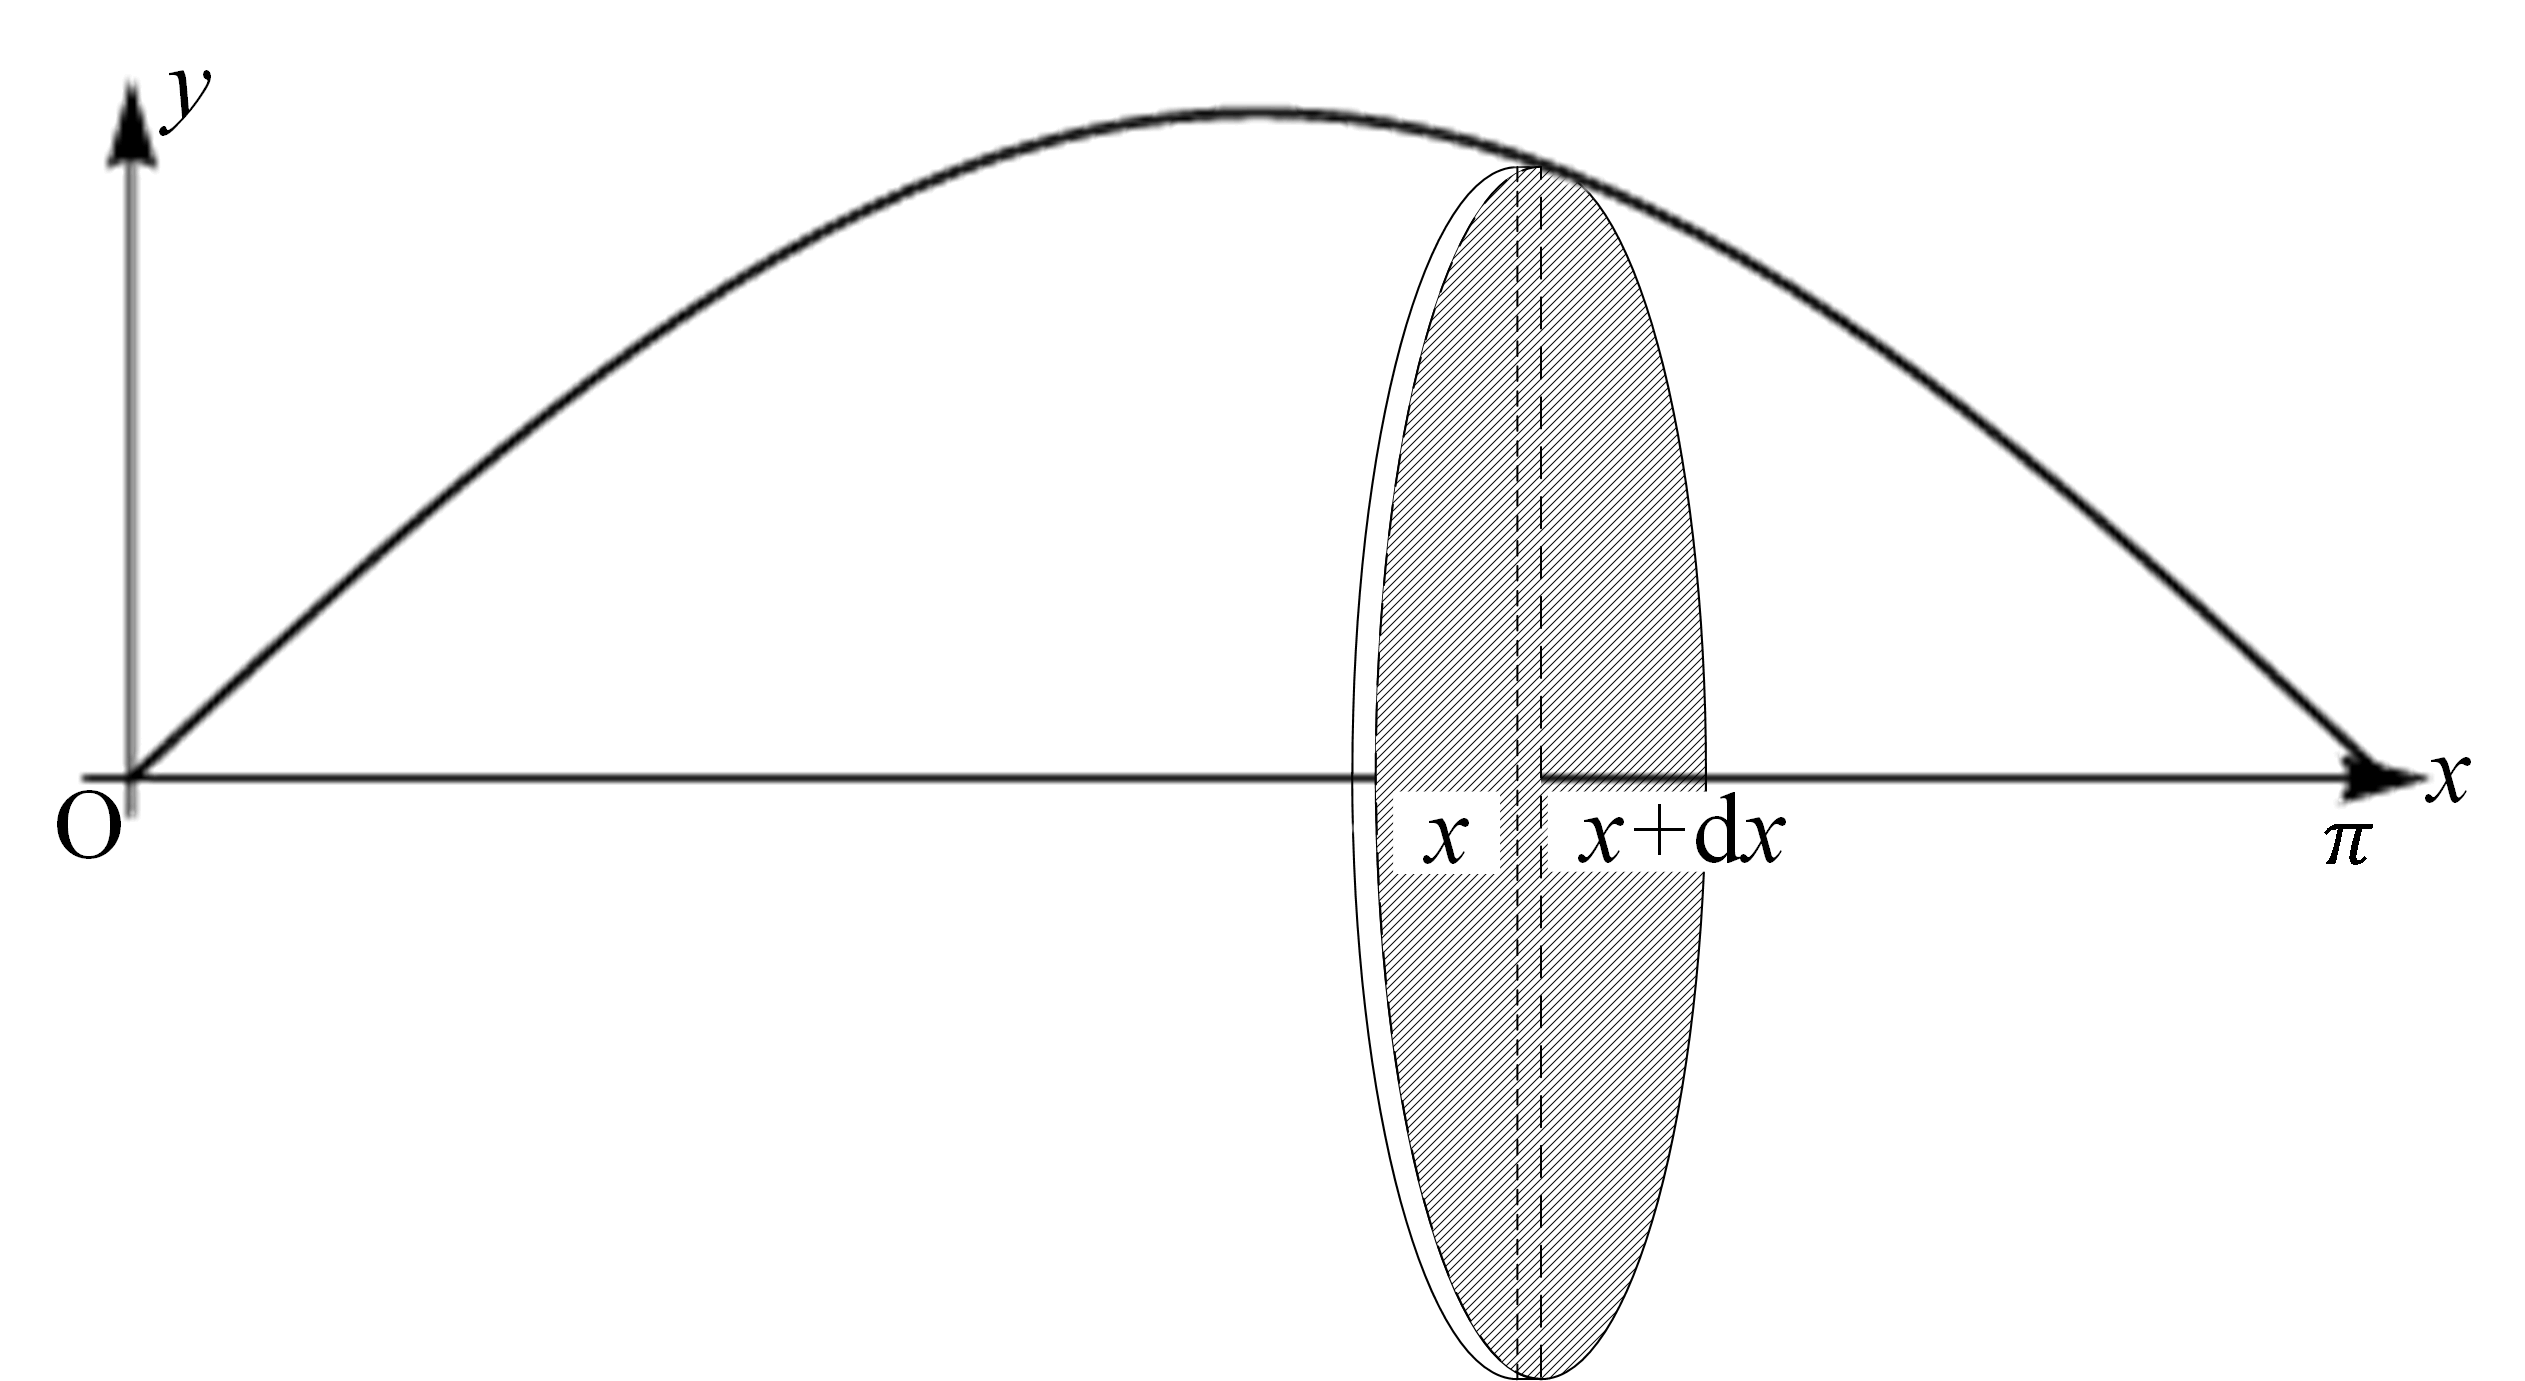
\includegraphics[height=0.2\textheight]{F:/life/2018AutumnTA/Exercises/11/Fig5-6-1-3.png} }}
%    \subfloat[]{\label{5-6-1-2} {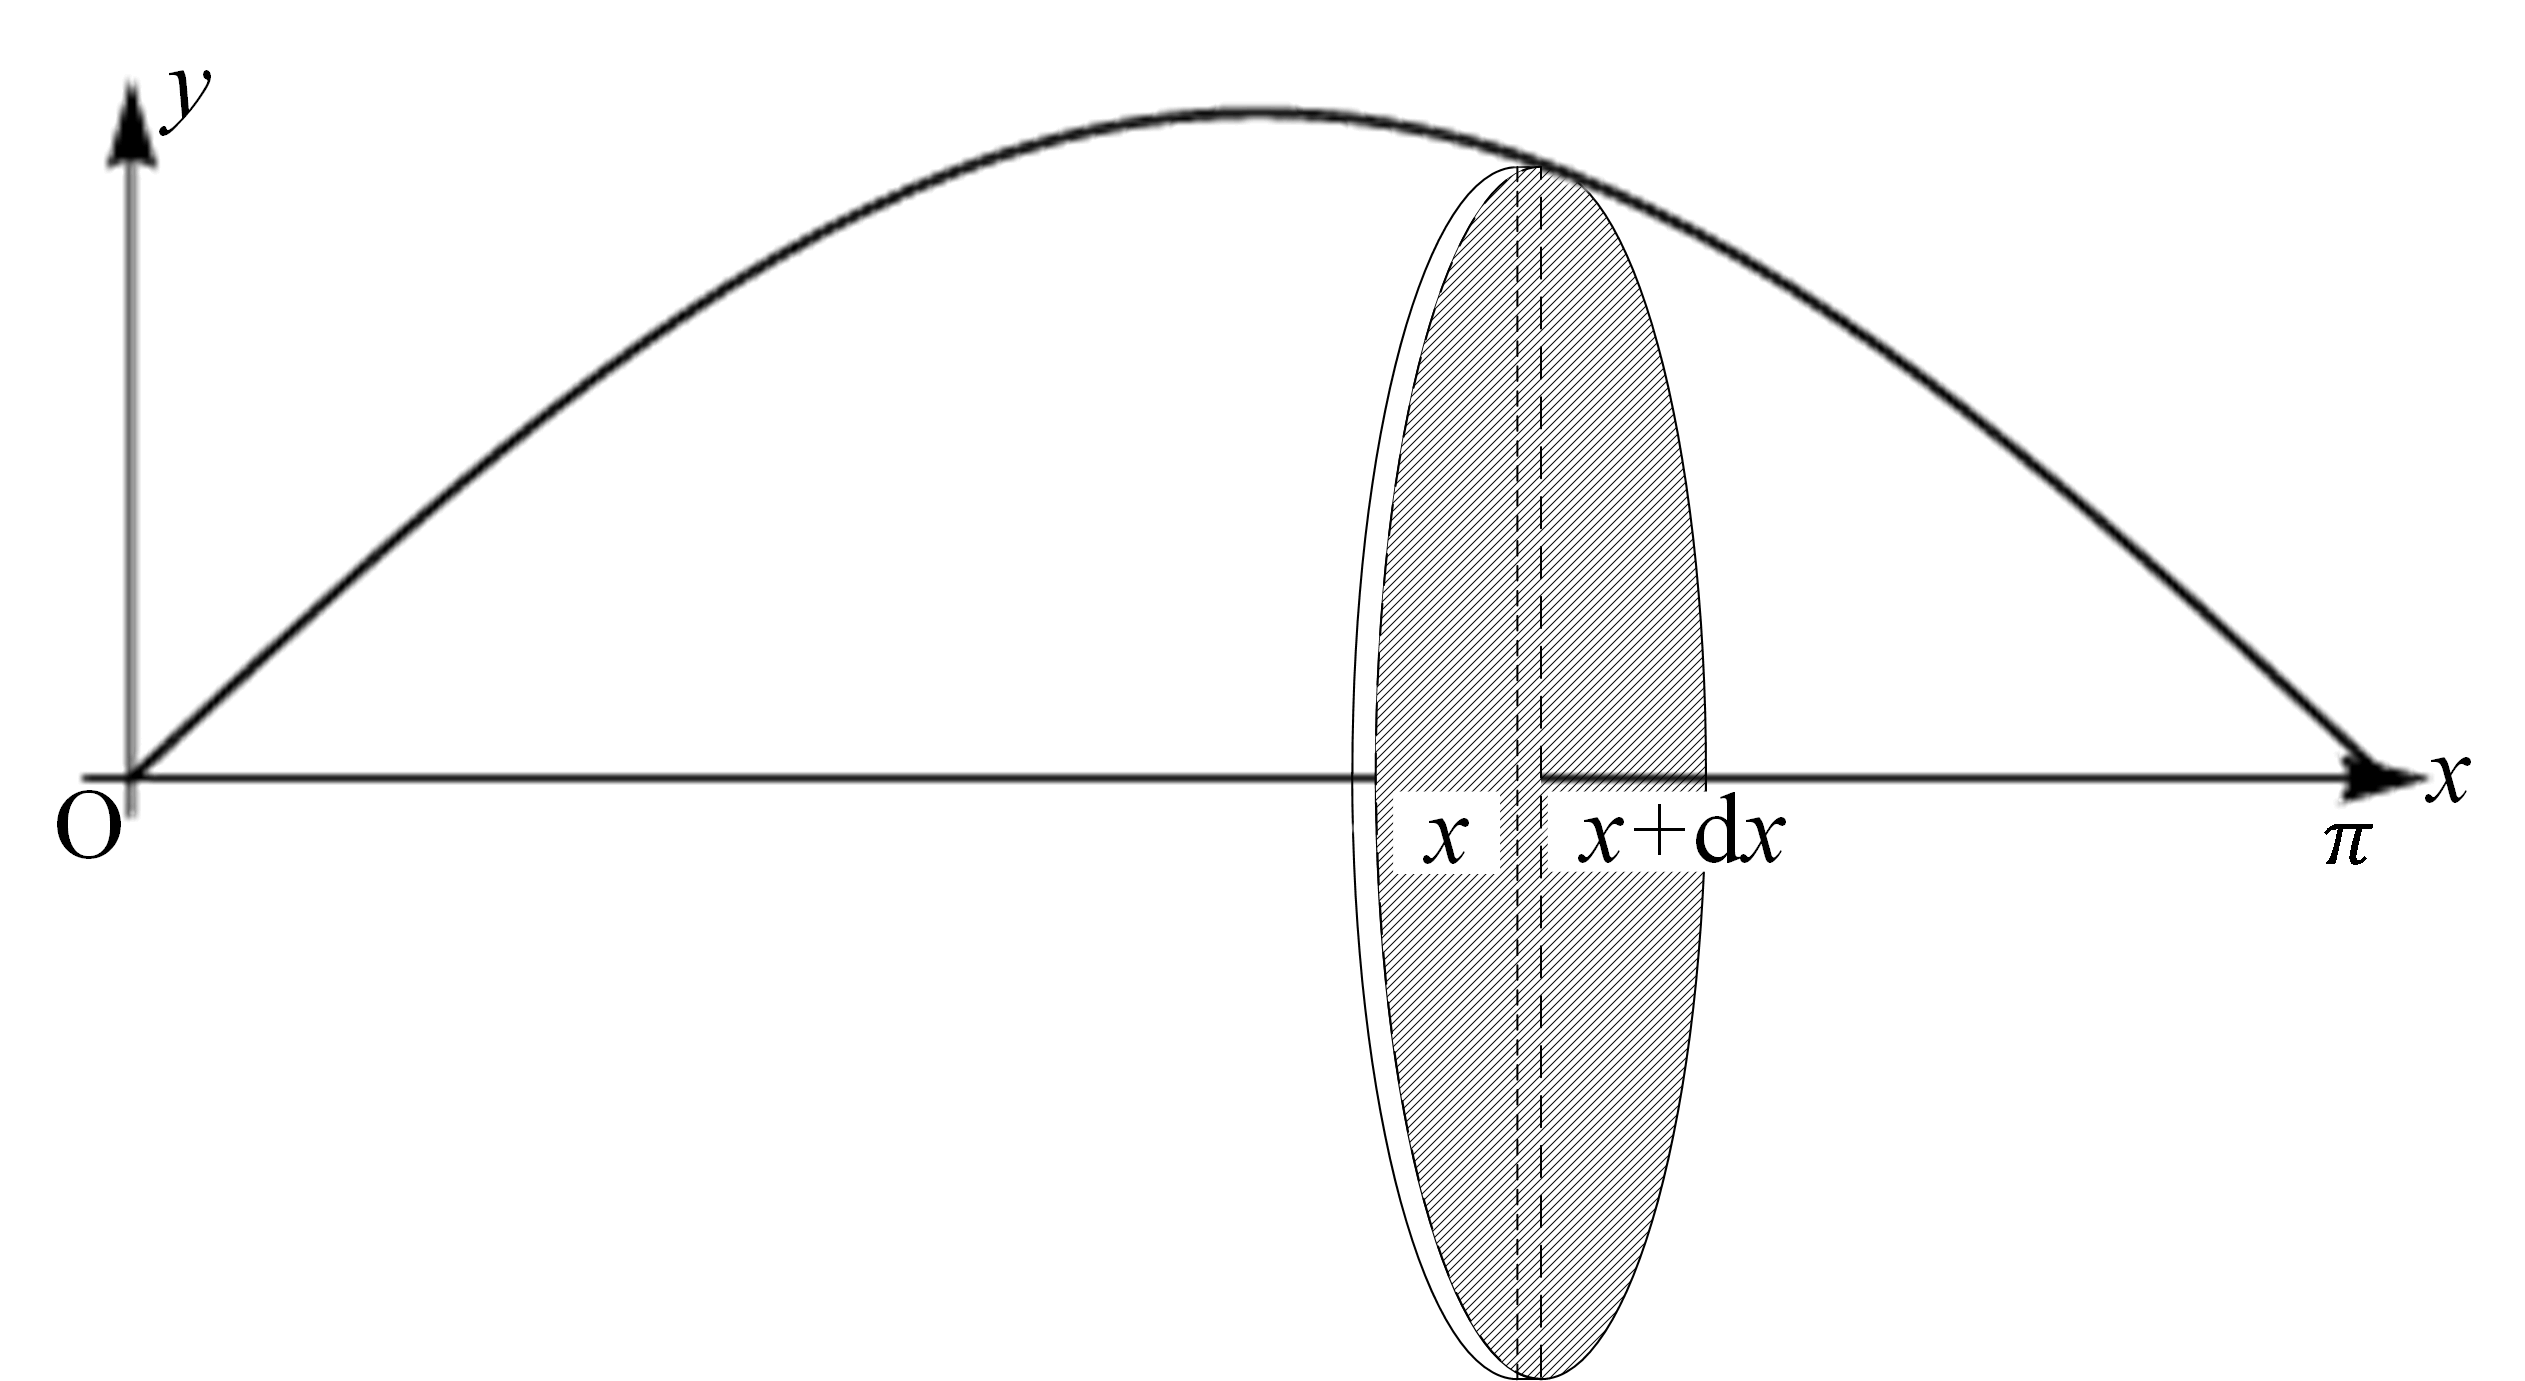
\includegraphics[height=0.2\textheight]{F:/life/2018AutumnTA/Exercises/11/Fig5-6-1-3.png} }}
\end{center}
\caption{习题7.5 6.(1)题图示}
\label{5-6-1}
\end{figure}
旋转体的体积为
\[V=\int_0^\pi\pi y^2\mathrm dx=\int_0^\pi\pi \sin^2x\mathrm dx=2\pi\int_0^{\frac\pi2}\sin^2x\mathrm dx=2\pi\frac12\frac\pi2=\frac{\pi^2}2.\]

(2)$\because x^{\frac23}+y^{\frac23}=a^{\frac23}$

$\therefore$曲线$y=y(x)$关于$x$轴和$y$轴均对称,图形如图~\ref{6-2-a}所示,绕$y$轴旋转得到的旋转体如图~\ref{6-2-b}所示. 
%\begin{figure}[H]
%\begin{center}
%\subfloat[]{\label{6-2-a} {\includegraphics[height=0.3\textheight]{Fig6-2.png} }}
%    \subfloat[]{\label{6-2-b} {\includegraphics[height=0.3\textheight]{Fig6-2-3D.png} }}
%%\begin{tabular}{cc}
%%\includegraphics[height=0.3\textheight]{Fig6-2.png}
%%&\includegraphics[height=0.3\textheight]{Fig6-2-3D.png}
%%\end{tabular}
%\end{center}
%\caption{6.(2)题图示}
%\end{figure}
求该旋转体的体积有以下两种方法:

方法1:对于如图~\ref{6-2-c}所示的切片体积积分,旋转体的体积可以表示为
\[\begin{split}
V&=\int_{-a}^a\pi x^2\mathrm dy=\int_{\frac32\pi}^{\frac12\pi}\pi a^2\cos^6t3a\sin^2t\cos t\mathrm dt=3\pi a^3\int_{\frac32\pi}^{\frac12\pi}(1-\sin^2t)^3\sin^2t\mathrm d\sin t\\
&=3\pi a^3\int_{\frac32\pi}^{\frac12\pi}(1-3\sin^2t+3\sin^4t-\sin^6t)\sin^2t\mathrm d\sin t\\
&=3\pi a^3\int_{\frac32\pi}^{\frac12\pi}(\sin^2t-3\sin^4t+3\sin^6t-\sin^8t)\mathrm d\sin t\\
&=3\pi a^3(\frac13\sin^3t-\frac35\sin^5t+\frac37\sin^7t-\frac19\sin^9t)\Big|_{\frac32\pi}^{\frac12\pi}\\
&=3\pi a^3(\frac13\cdot2-\frac35\cdot2+\frac37\cdot2-\frac19\cdot2)\\
&=\frac{32}{105}\pi a^3.
\end{split}\]

方法2:对于如图~\ref{6-2-d}所示的圆柱壳体积积分,旋转体的体积可以表示为
\[\begin{split}
V&=\int_0^{a}2\pi x\cdot2y\mathrm dx=-\int_{\frac12\pi}^02\pi a\cos^3t\cdot2a\sin^3t\cdot3a\cos^2t\sin t\mathrm dt\\
&=-12\pi a^3\int_{\frac12\pi}^0\sin^4t\cos^4t\mathrm d\sin t\\
&=12\pi a^3\int_0^{\frac12\pi}\sin^4t(1-\sin^2t)^2\mathrm d\sin t\\
&=12\pi a^3\int_0^{\frac12\pi}\sin^4t(1-2\sin^2t+\sin^4t)\mathrm d\sin t\\
&=12\pi a^3\int_0^{\frac12\pi}(\sin^4t-2\sin^6t+\sin^8t)\mathrm d\sin t\\
&=12\pi a^3(\frac15\sin^5t-\frac27\sin^7t+\frac19\sin^9t)\Big|_0^{\frac\pi2}\\
&=12\pi a^3(\frac15-\frac27+\frac19)\\
&=\frac{32}{105}\pi a^3.
\end{split}\]
\begin{figure}[H]
\begin{center}
\subfloat[]{\label{6-2-a}
{\includegraphics[height=0.3\textheight]{F:/life/2018AutumnTA/Exercises/11/Fig6-2.png} }}
    \subfloat[]{\label{6-2-b} {\includegraphics[height=0.3\textheight]{F:/life/2018AutumnTA/Exercises/11/Fig6-2-3D.png} }}\\
    
    \subfloat[]{\label{6-2-c} {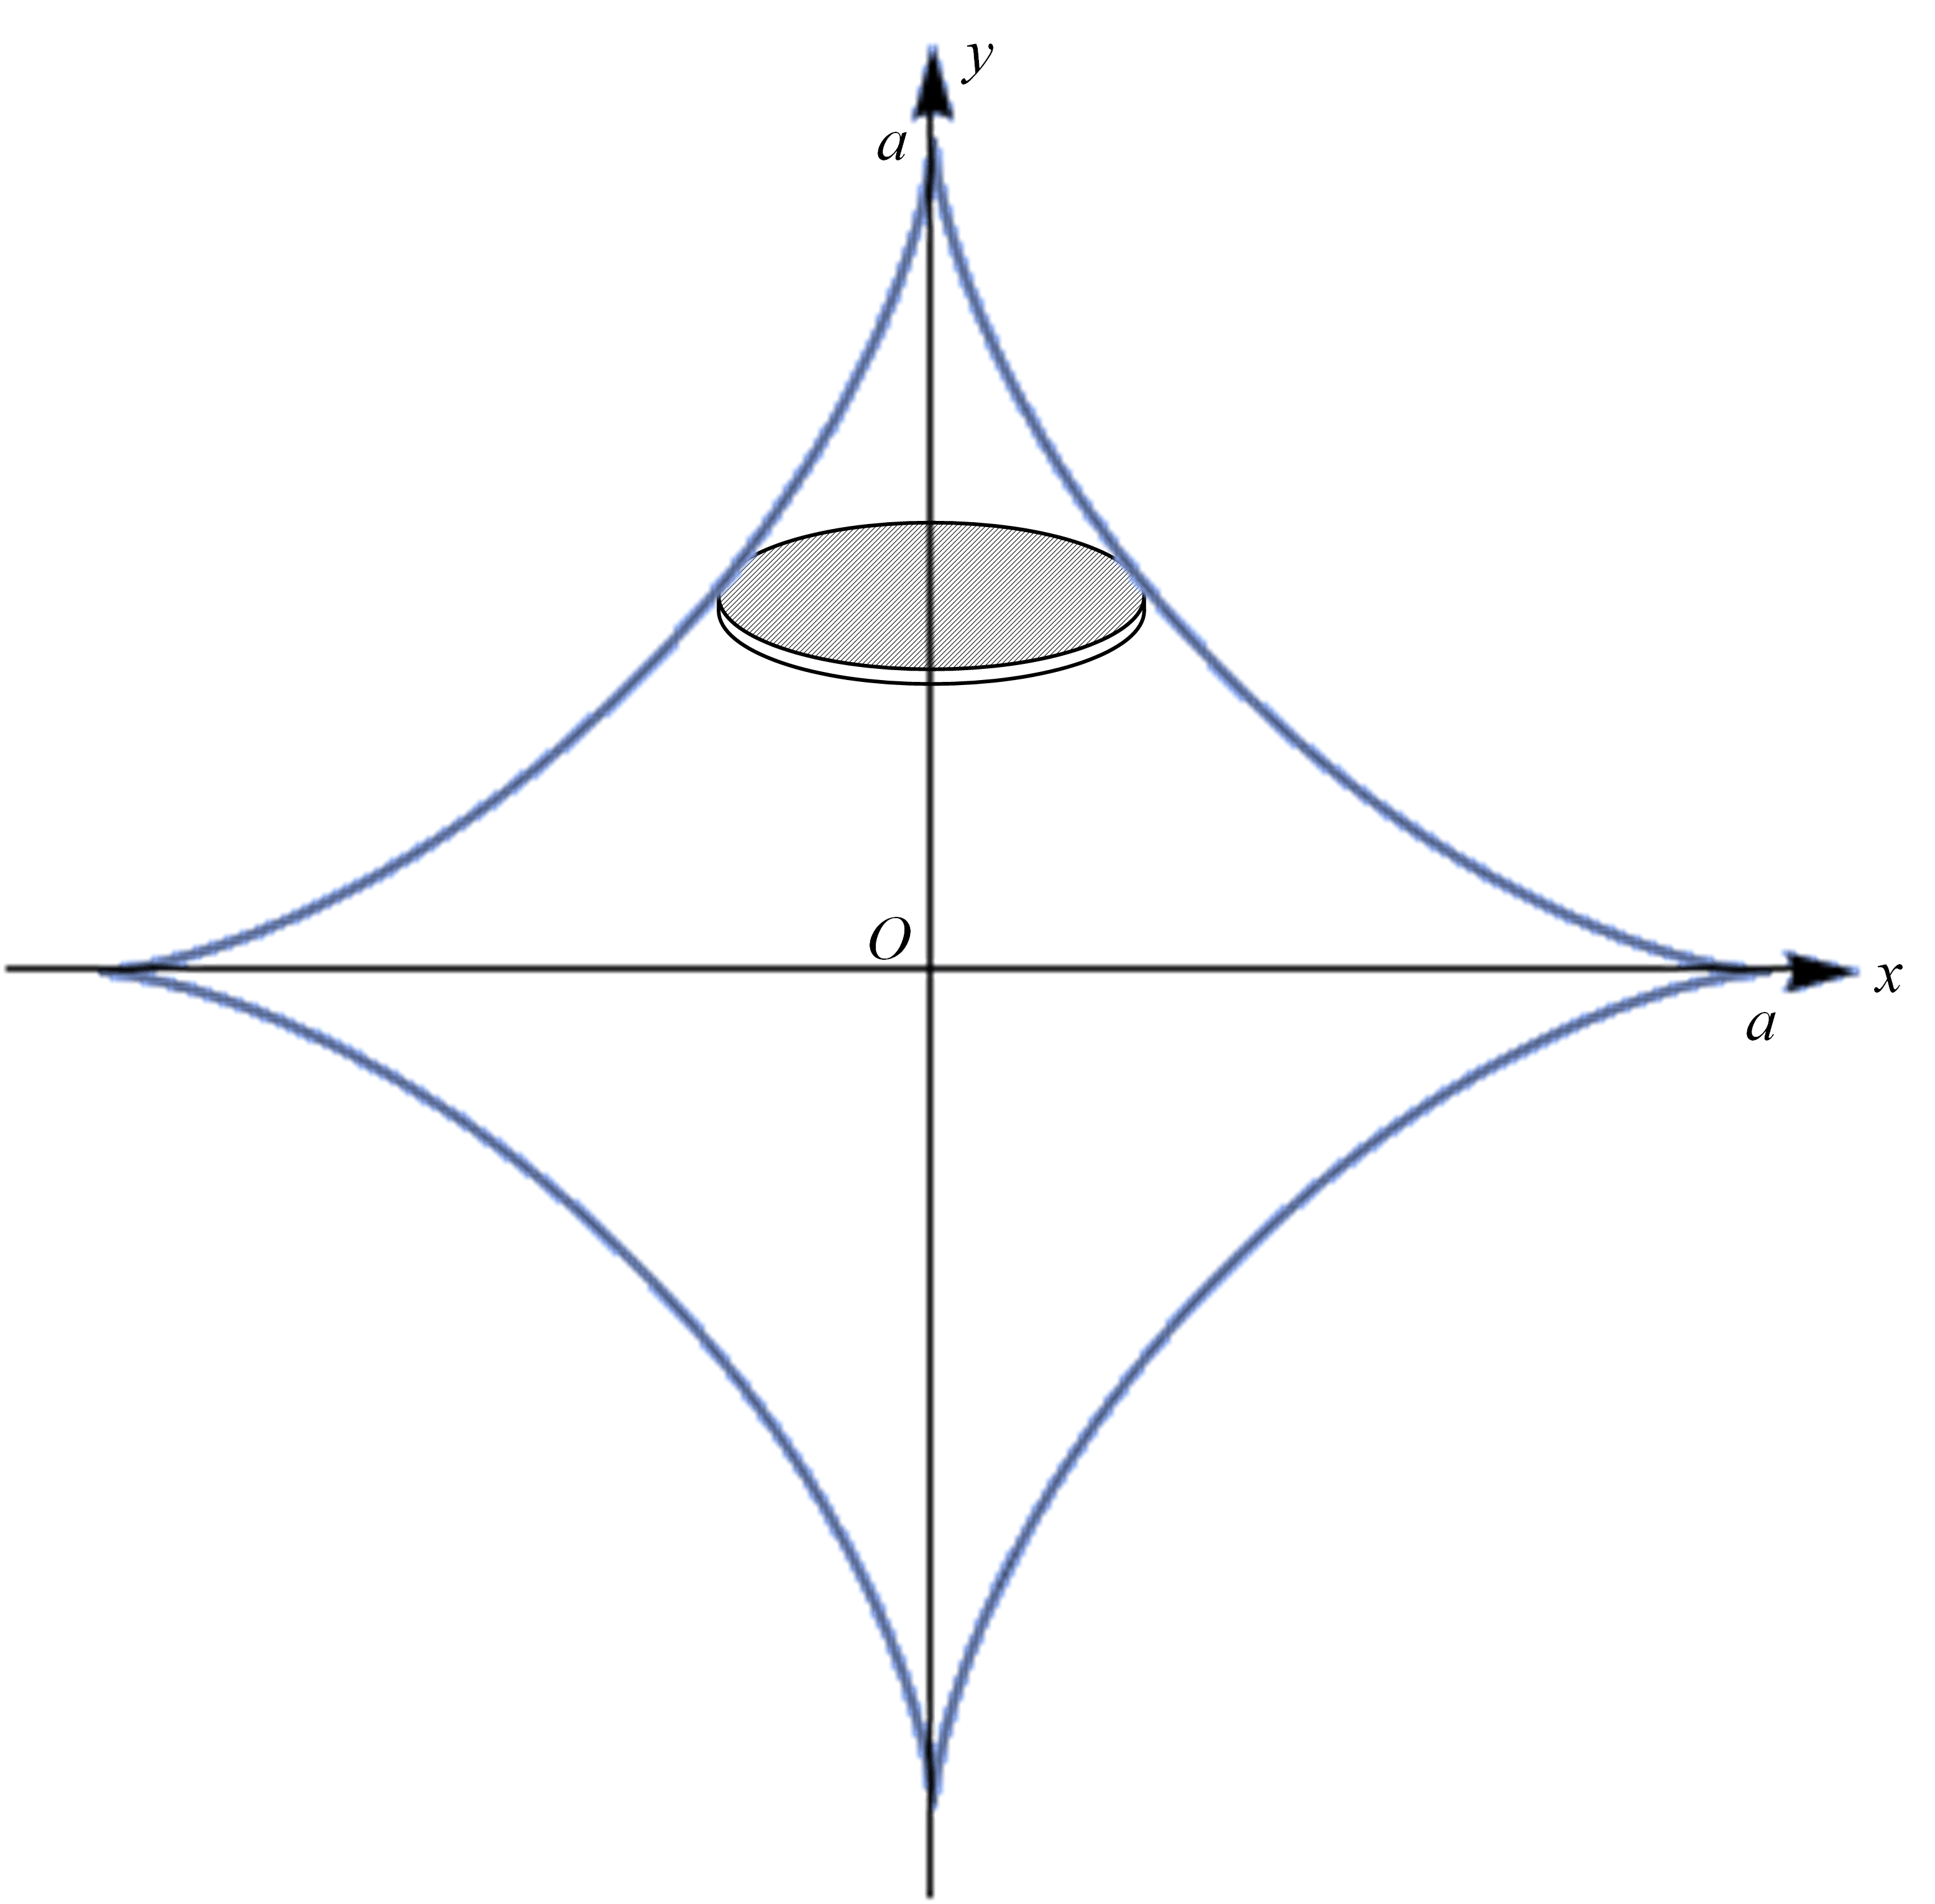
\includegraphics[height=0.3\textheight]{F:/life/2018AutumnTA/Exercises/11/Fig6-2-1.png} }}
    \subfloat[]{\label{6-2-d} {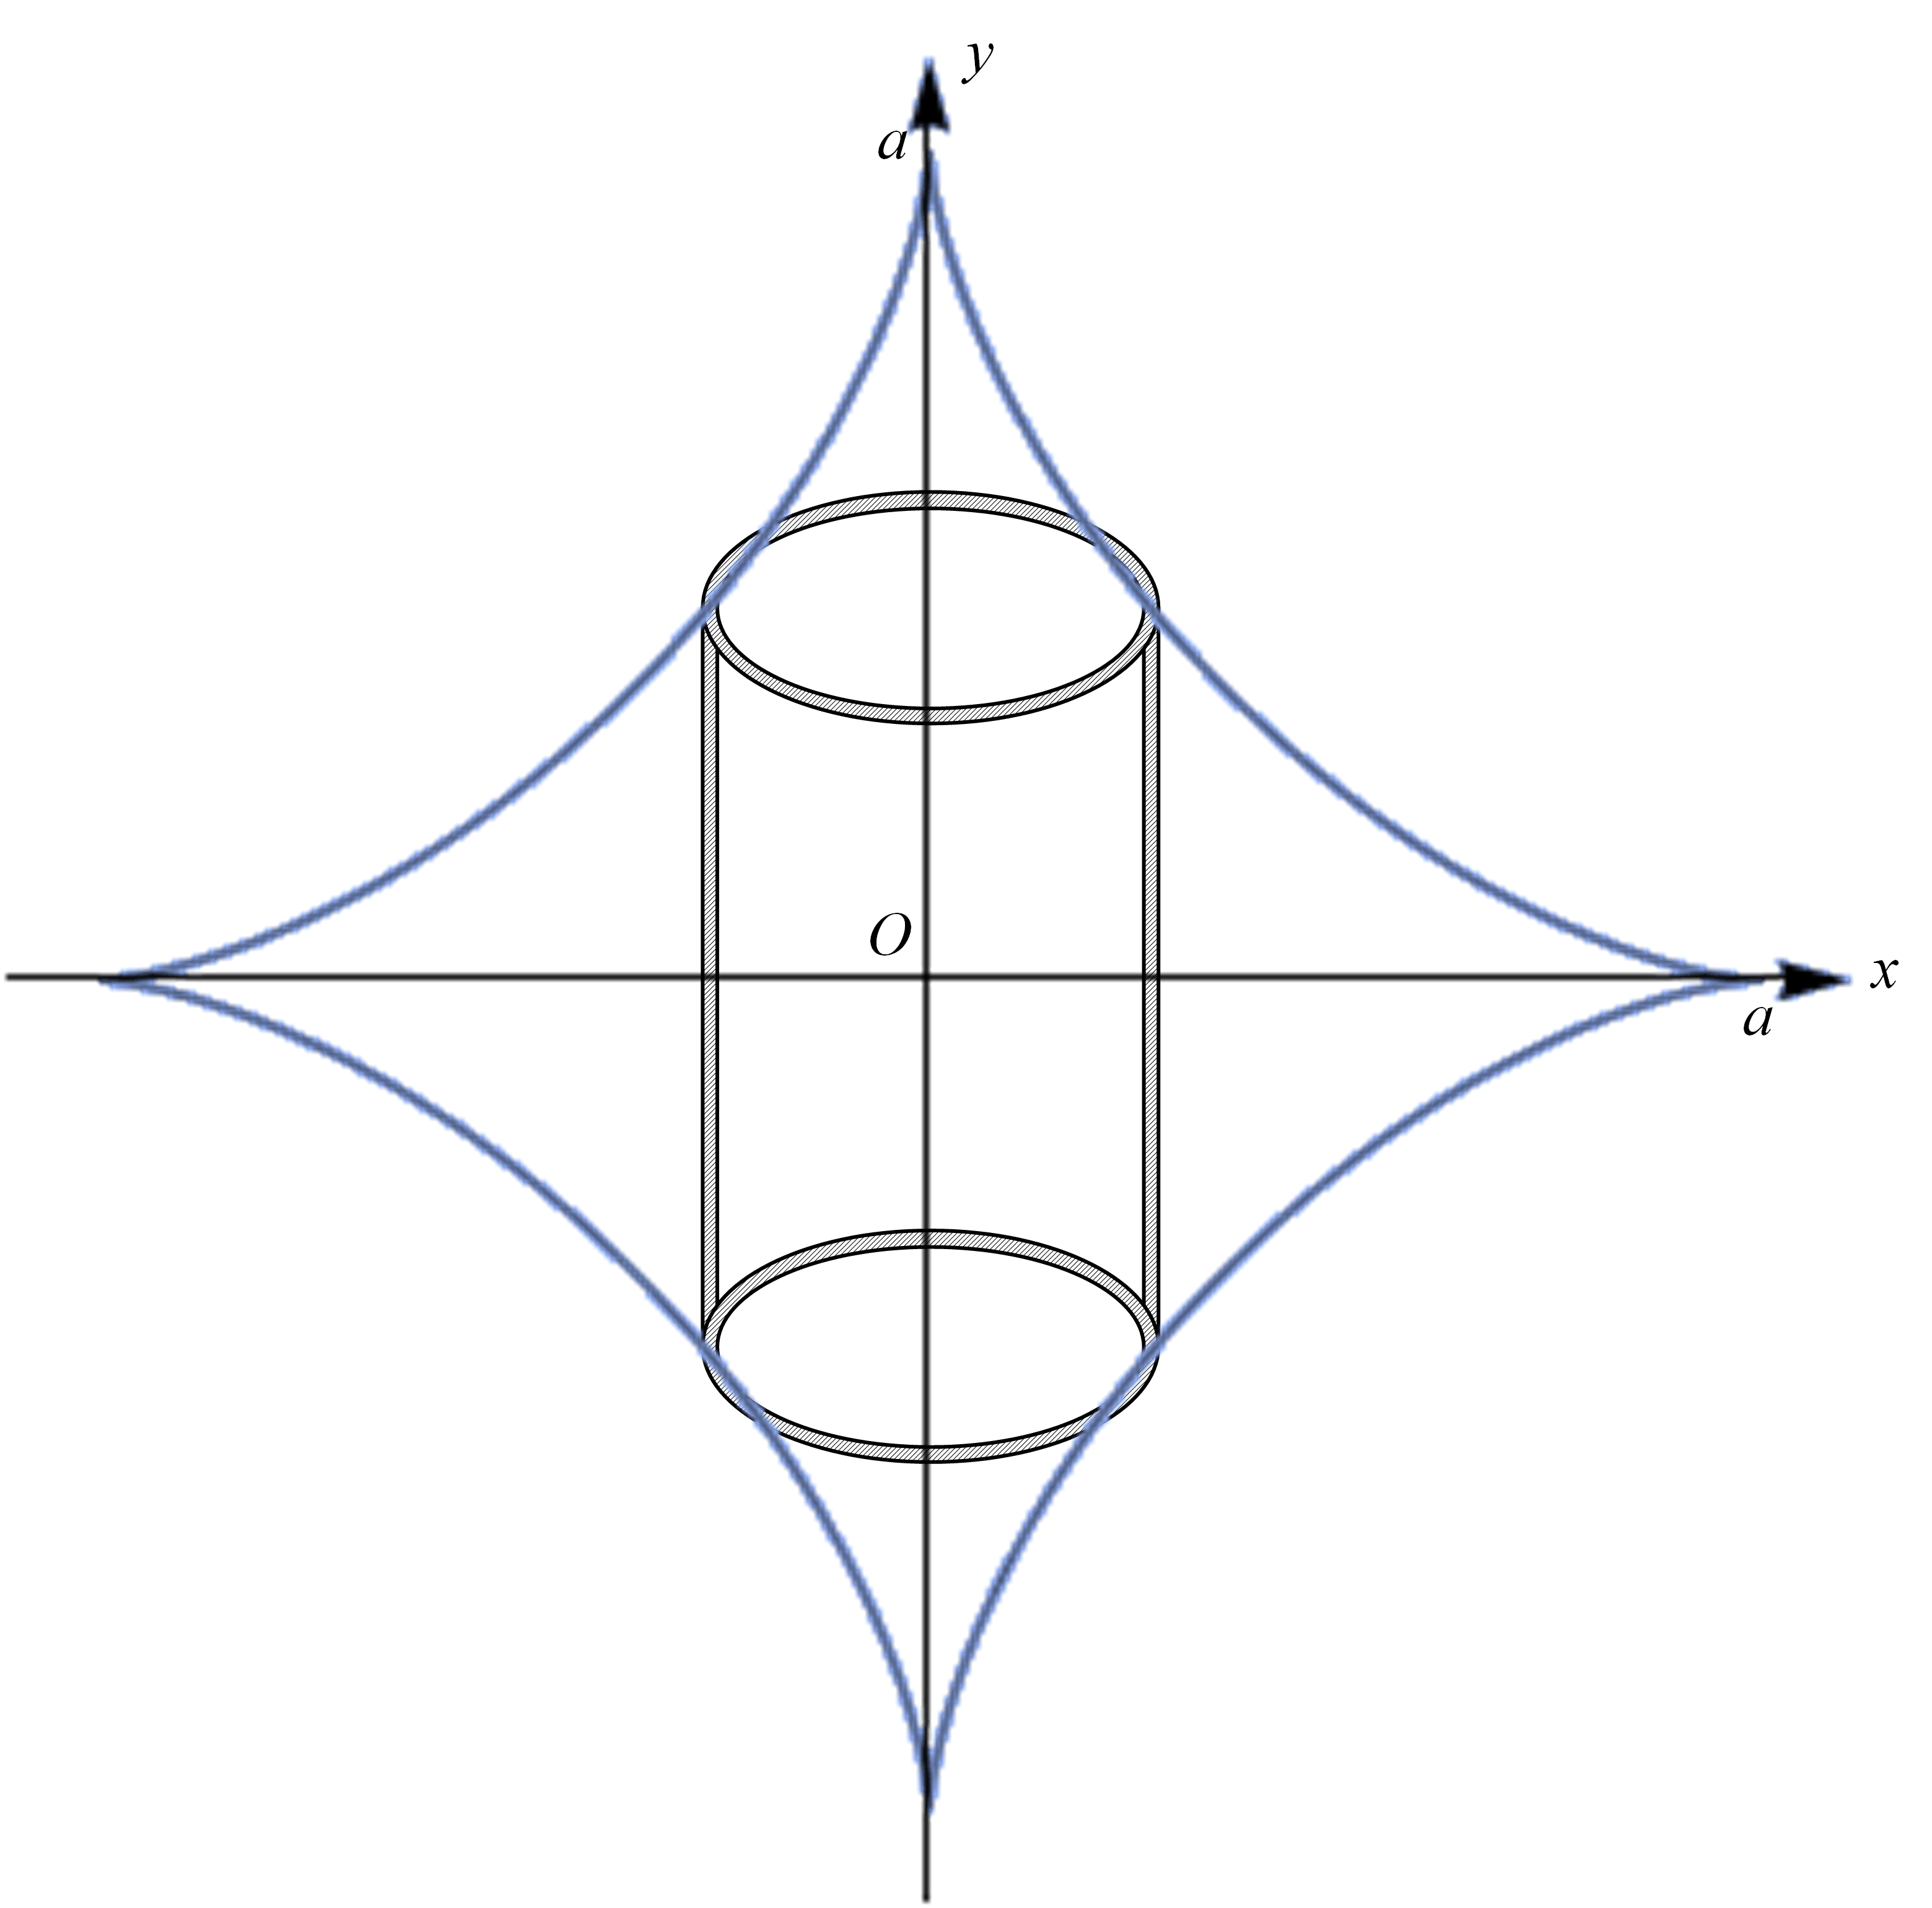
\includegraphics[height=0.3\textheight]{F:/life/2018AutumnTA/Exercises/11/Fig6-2-2.png} }}
%\begin{tabular}{cc}
%\includegraphics[height=0.3\textheight]{Fig6-2.png}
%&\includegraphics[height=0.3\textheight]{Fig6-2-3D.png}
%\end{tabular}
\end{center}
\caption{6.(2)题图示}
\end{figure}
(3)曲线形状如图~\ref{6-3-a}所示,绕$x$轴转动后得到的旋转体如图~\ref{6-3-b}所示. 设曲线最左侧的两点的横坐标为$x_0$,其中在$x$轴上方的点对应的极角为$\theta_0$,这两点将曲线分成黑色和红色的两部分,该旋转体可视为图~\ref{6-3-c}中的黑色轮廓绕$x$轴转动得到的旋转体剪去红色轮廓绕$x$轴转动得到的旋转体.

黑色轮廓绕$x$轴转动得到的旋转体的体积为
\[\begin{split}
V_1=\int_{x_0}^{2a}\pi y^2\mathrm dx=\int_{\theta_0}^0\pi[a(1+\cos\theta)\sin\theta]^2\mathrm d[a(1+\cos\theta)\cos\theta]
\end{split}\]
红色轮廓绕$x$轴转动得到的旋转体的体积为
\[\begin{split}
V_2=\int_{x_0}^{0}\pi y^2\mathrm dx=\int_{\theta_0}^\pi\pi[a(1+\cos\theta)\sin\theta]^2\mathrm d[a(1+\cos\theta)\cos\theta]
\end{split}\]
则原曲线绕$x$轴转动得到的旋转体的体积为
\[\begin{split}
V&=V_1-V_2\\
&=\int_{\theta_0}^0\pi[a(1+\cos\theta)\sin\theta]^2\mathrm d[a(1+\cos\theta)\cos\theta]-\int_{\theta_0}^\pi\pi[a(1+\cos\theta)\sin\theta]^2\mathrm d[a(1+\cos\theta)\cos\theta]\\
&=\int_{\theta_0}^0\pi[a(1+\cos\theta)\sin\theta]^2\mathrm d[a(1+\cos\theta)\cos\theta]+\int_\pi^{\theta_0}\pi[a(1+\cos\theta)\sin\theta]^2\mathrm d[a(1+\cos\theta)\cos\theta]\\
&=\int_\pi^0\pi[a(1+\cos\theta)\sin\theta]^2\mathrm d[a(1+\cos\theta)\cos\theta]\\
&=\pi a^2\int_\pi^0(1+\cos\theta)^2\sin^2\theta(-\sin\theta-2\cos\theta\sin\theta)\mathrm d\theta\\
&=\pi a^2\int_\pi^0(1+\cos\theta)^2(1-\cos^2\theta)(1+2\cos\theta)\mathrm d\cos\theta\\
&=\pi a^2\int_{-1}^1(1+u)^2(1-u^2)(1+2u)\mathrm du\\
&=\pi a^2\int_{-1}^1(1+4u+4u^2-2u^3-5u^4-2u^5)\mathrm du\\
&=\pi a^2(u+2u^2+\frac43u^3-\frac12u^4-u^5-\frac13u^6)\Big|_{-1}^1\\
&=\pi a^2(2+0+\frac43\cdot2-0-2-0)\\
&=\frac83\pi a^3
\end{split}\]
\begin{figure}[H]
\begin{center}
\subfloat[]{\label{6-3-a}
{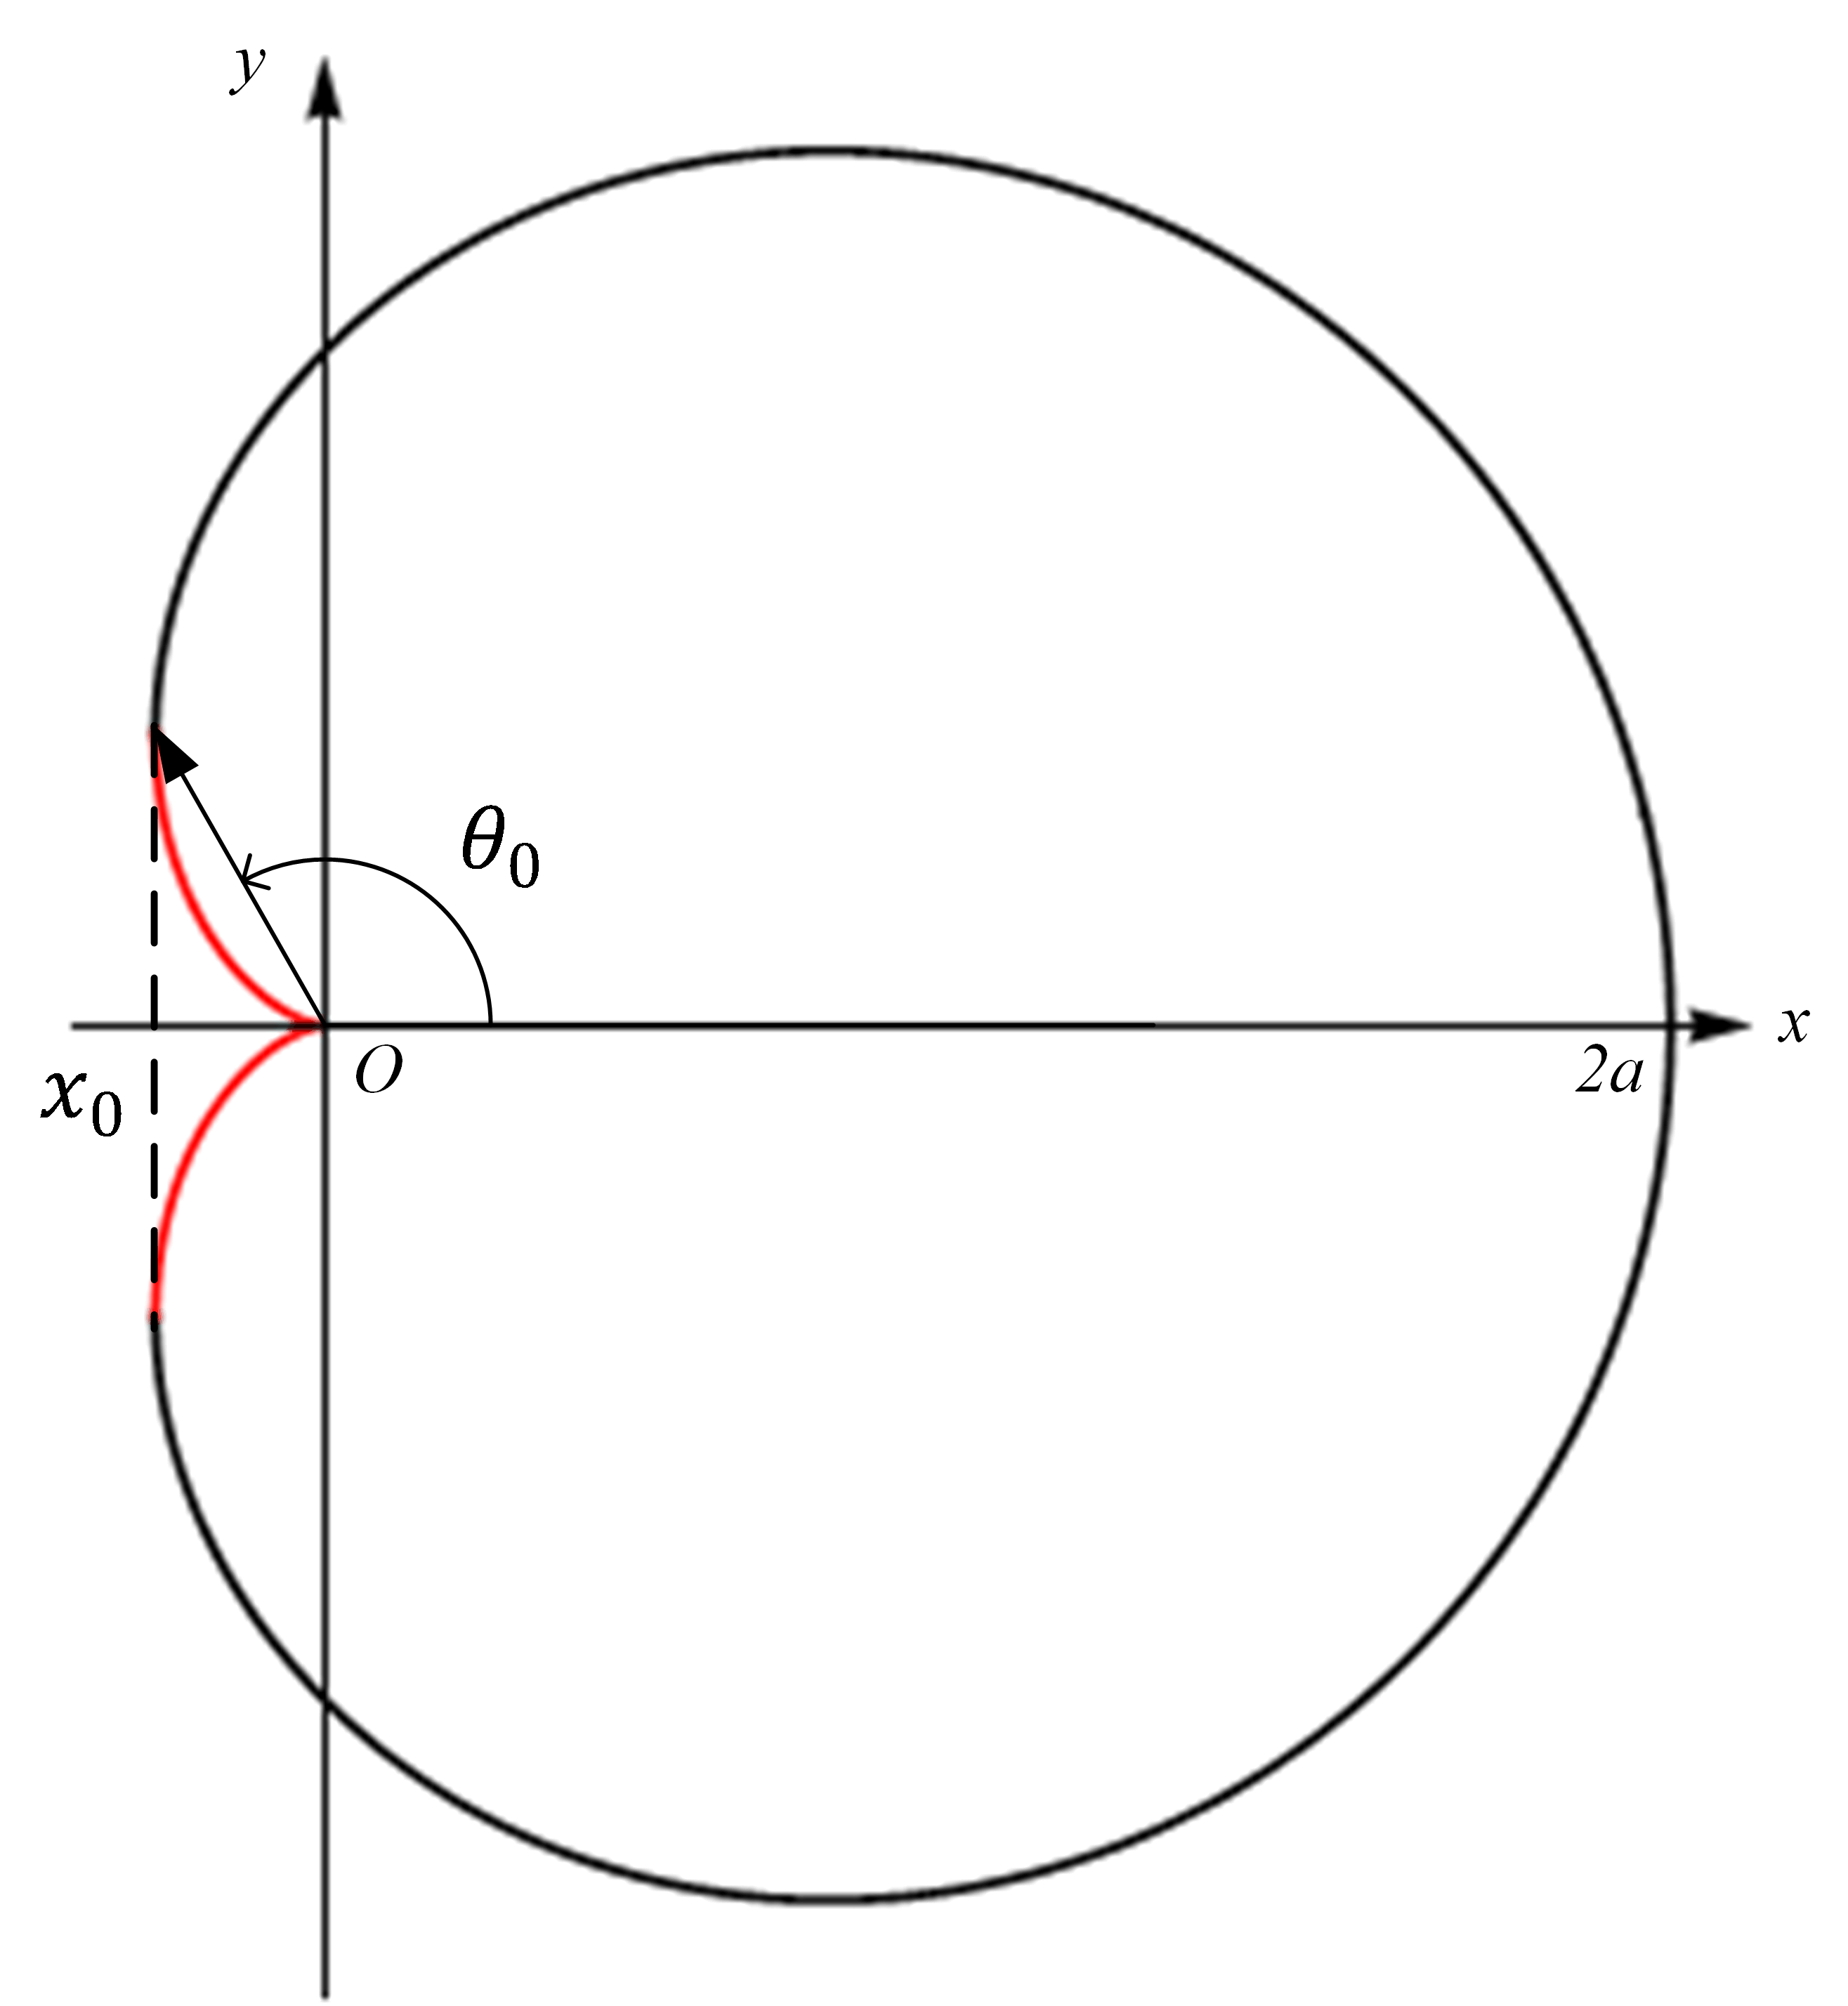
\includegraphics[height=0.3\textheight]{F:/life/2018AutumnTA/Exercises/11/Fig6-3.png} }}
    \subfloat[]{\label{6-3-b} {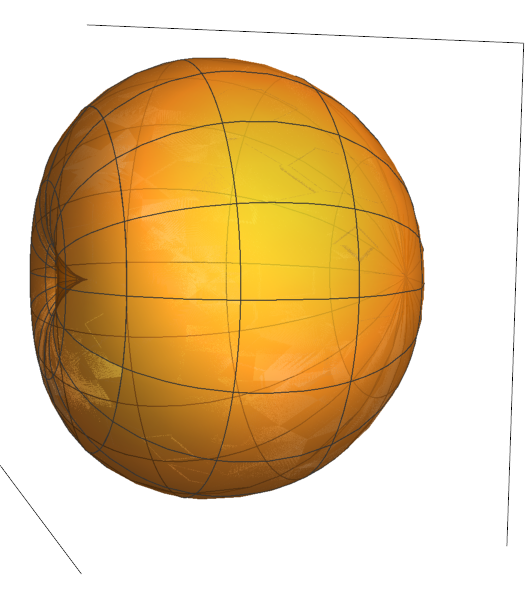
\includegraphics[height=0.3\textheight]{F:/life/2018AutumnTA/Exercises/11/Fig6-3-3D.png} }}\\
    \subfloat[]{\label{6-3-c} {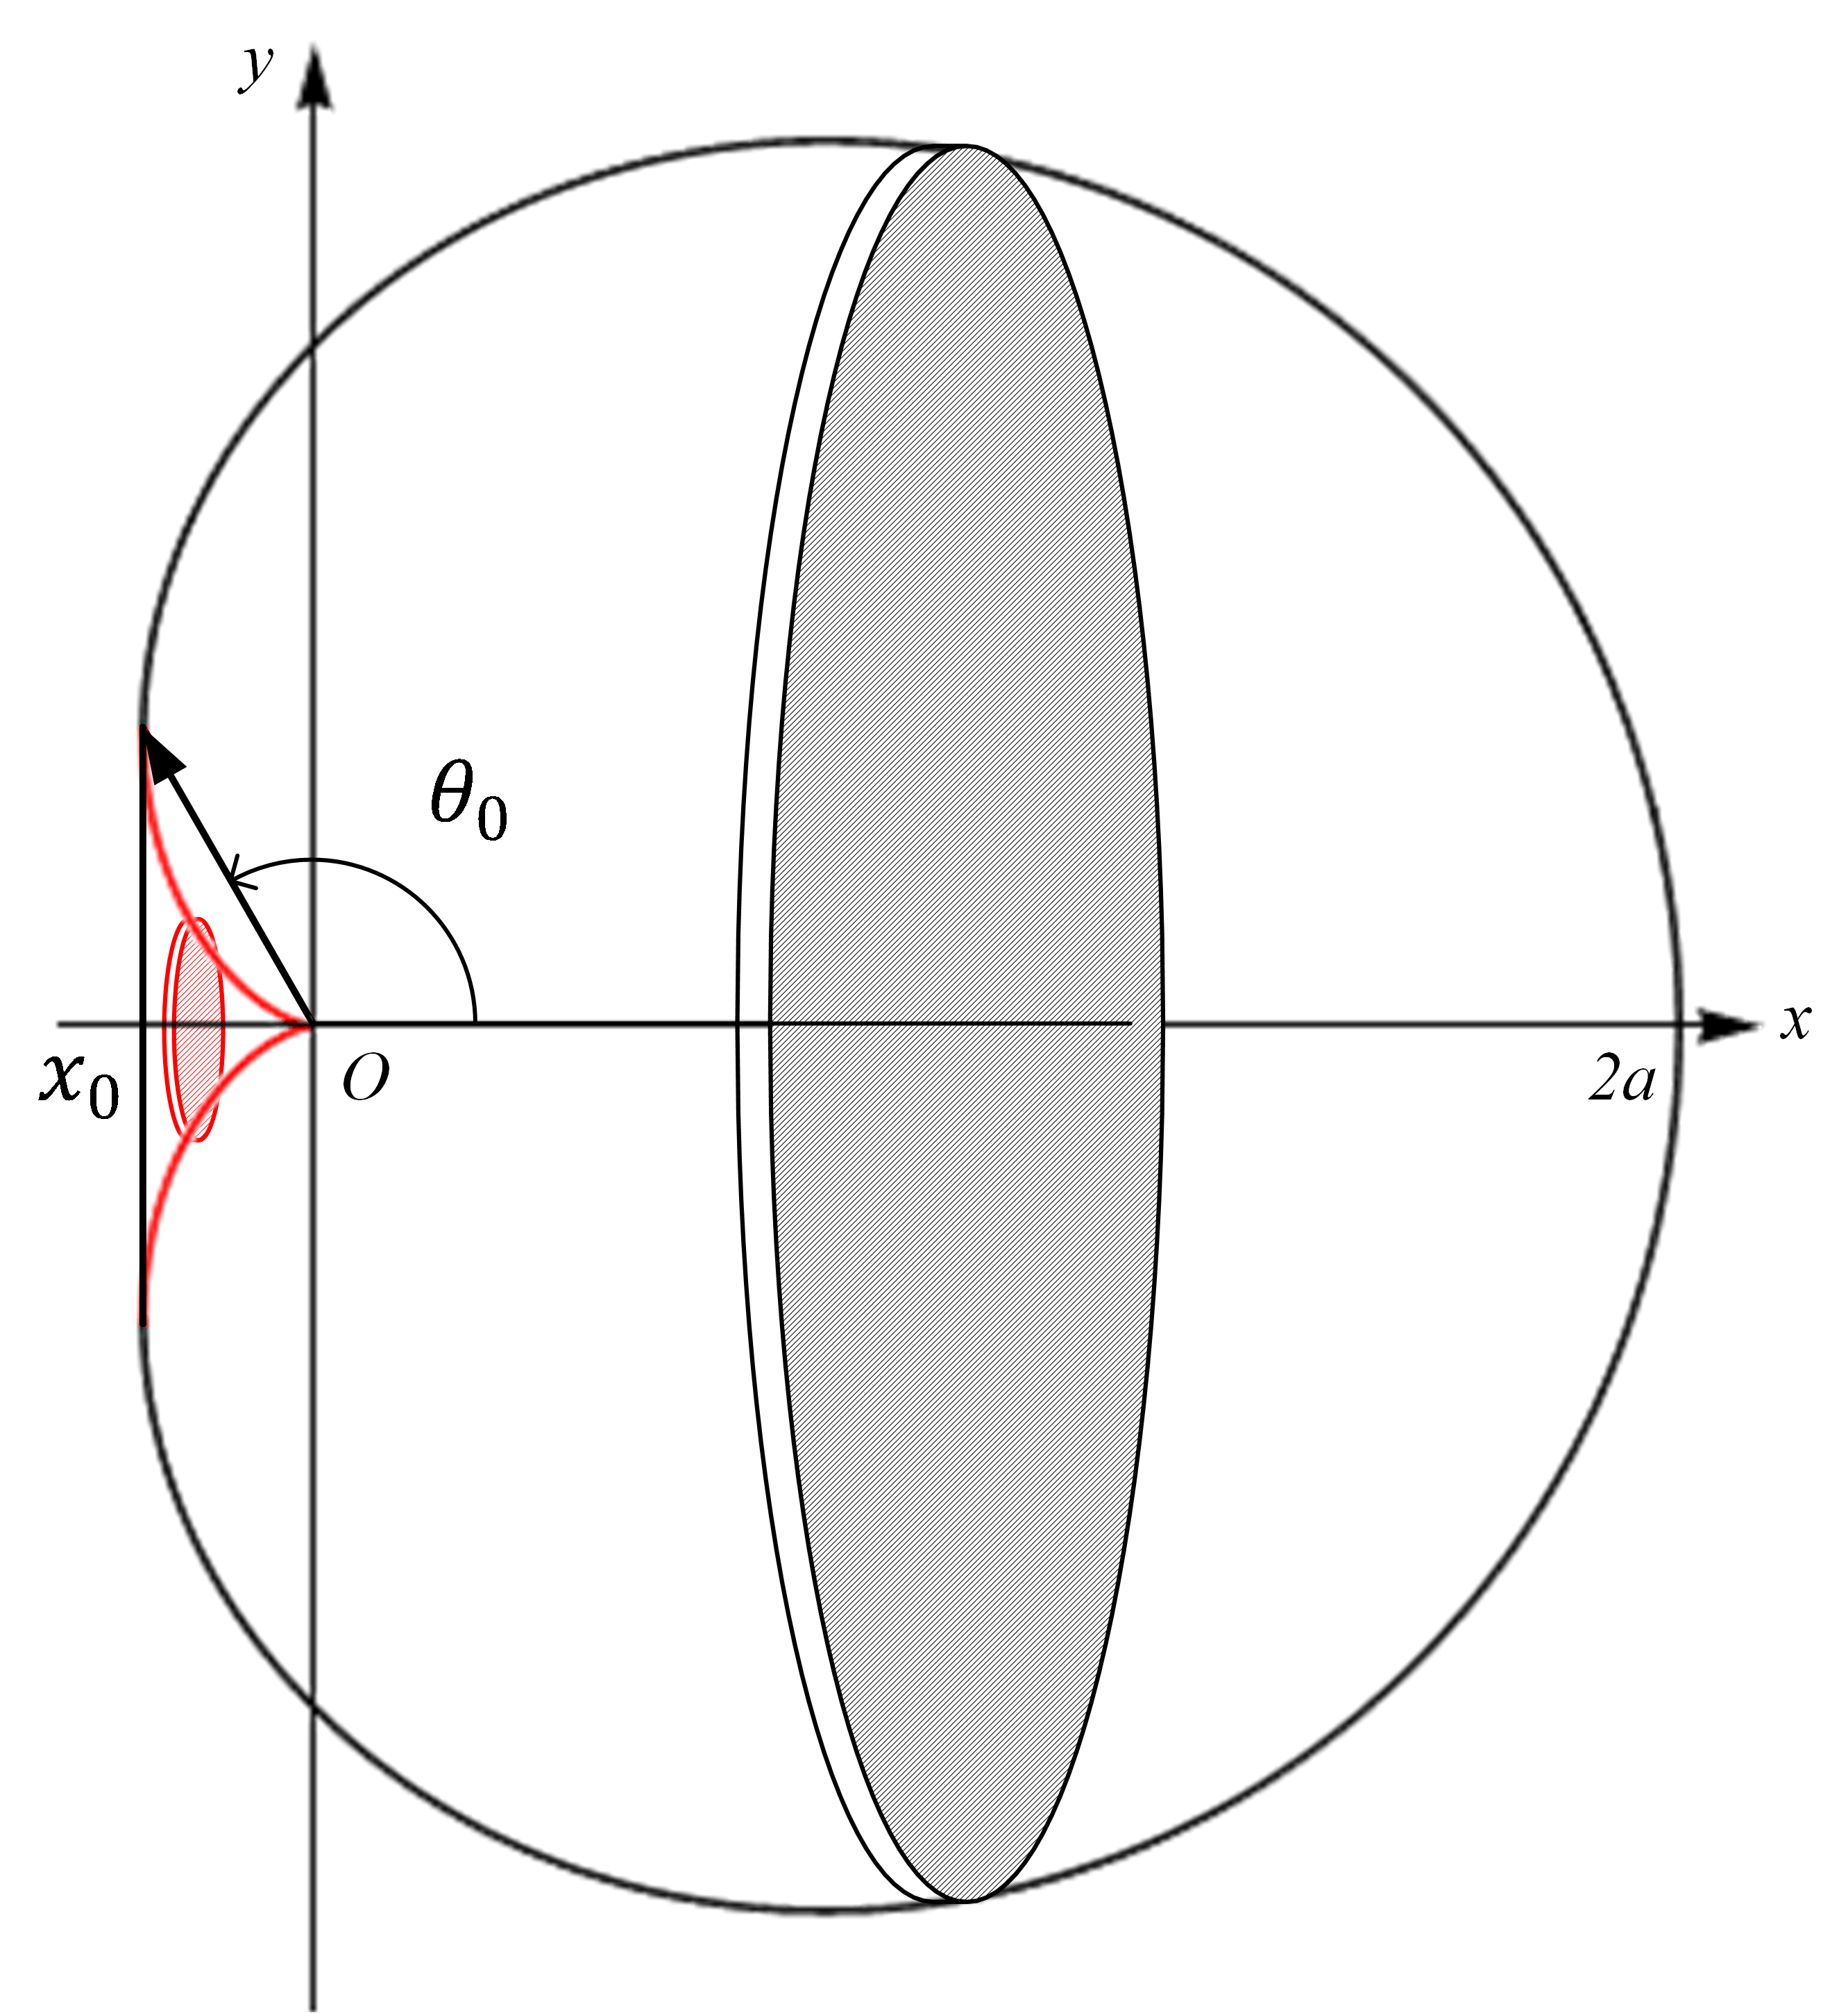
\includegraphics[height=0.3\textheight]{F:/life/2018AutumnTA/Exercises/11/Fig6-3-1.png} }}
\end{center}
\caption{6.(3)题图示}
\end{figure}
\item求下列旋转曲面的面积:
\newline
(1)$y^2=2px+a,0\leq x\leq a,a>1$绕$x$轴;
\newline
(2)$\begin{cases}
x=a(t-\sin t),\\
y=a(1-\cos t),
\end{cases}0\leq t\leq 2\pi$绕$x$轴.

解:(1)该旋转曲面的形状如图~\ref{5-7-1-2}所示,
\begin{figure}[H]
\begin{center}
\subfloat[]{\label{5-7-1-1}
{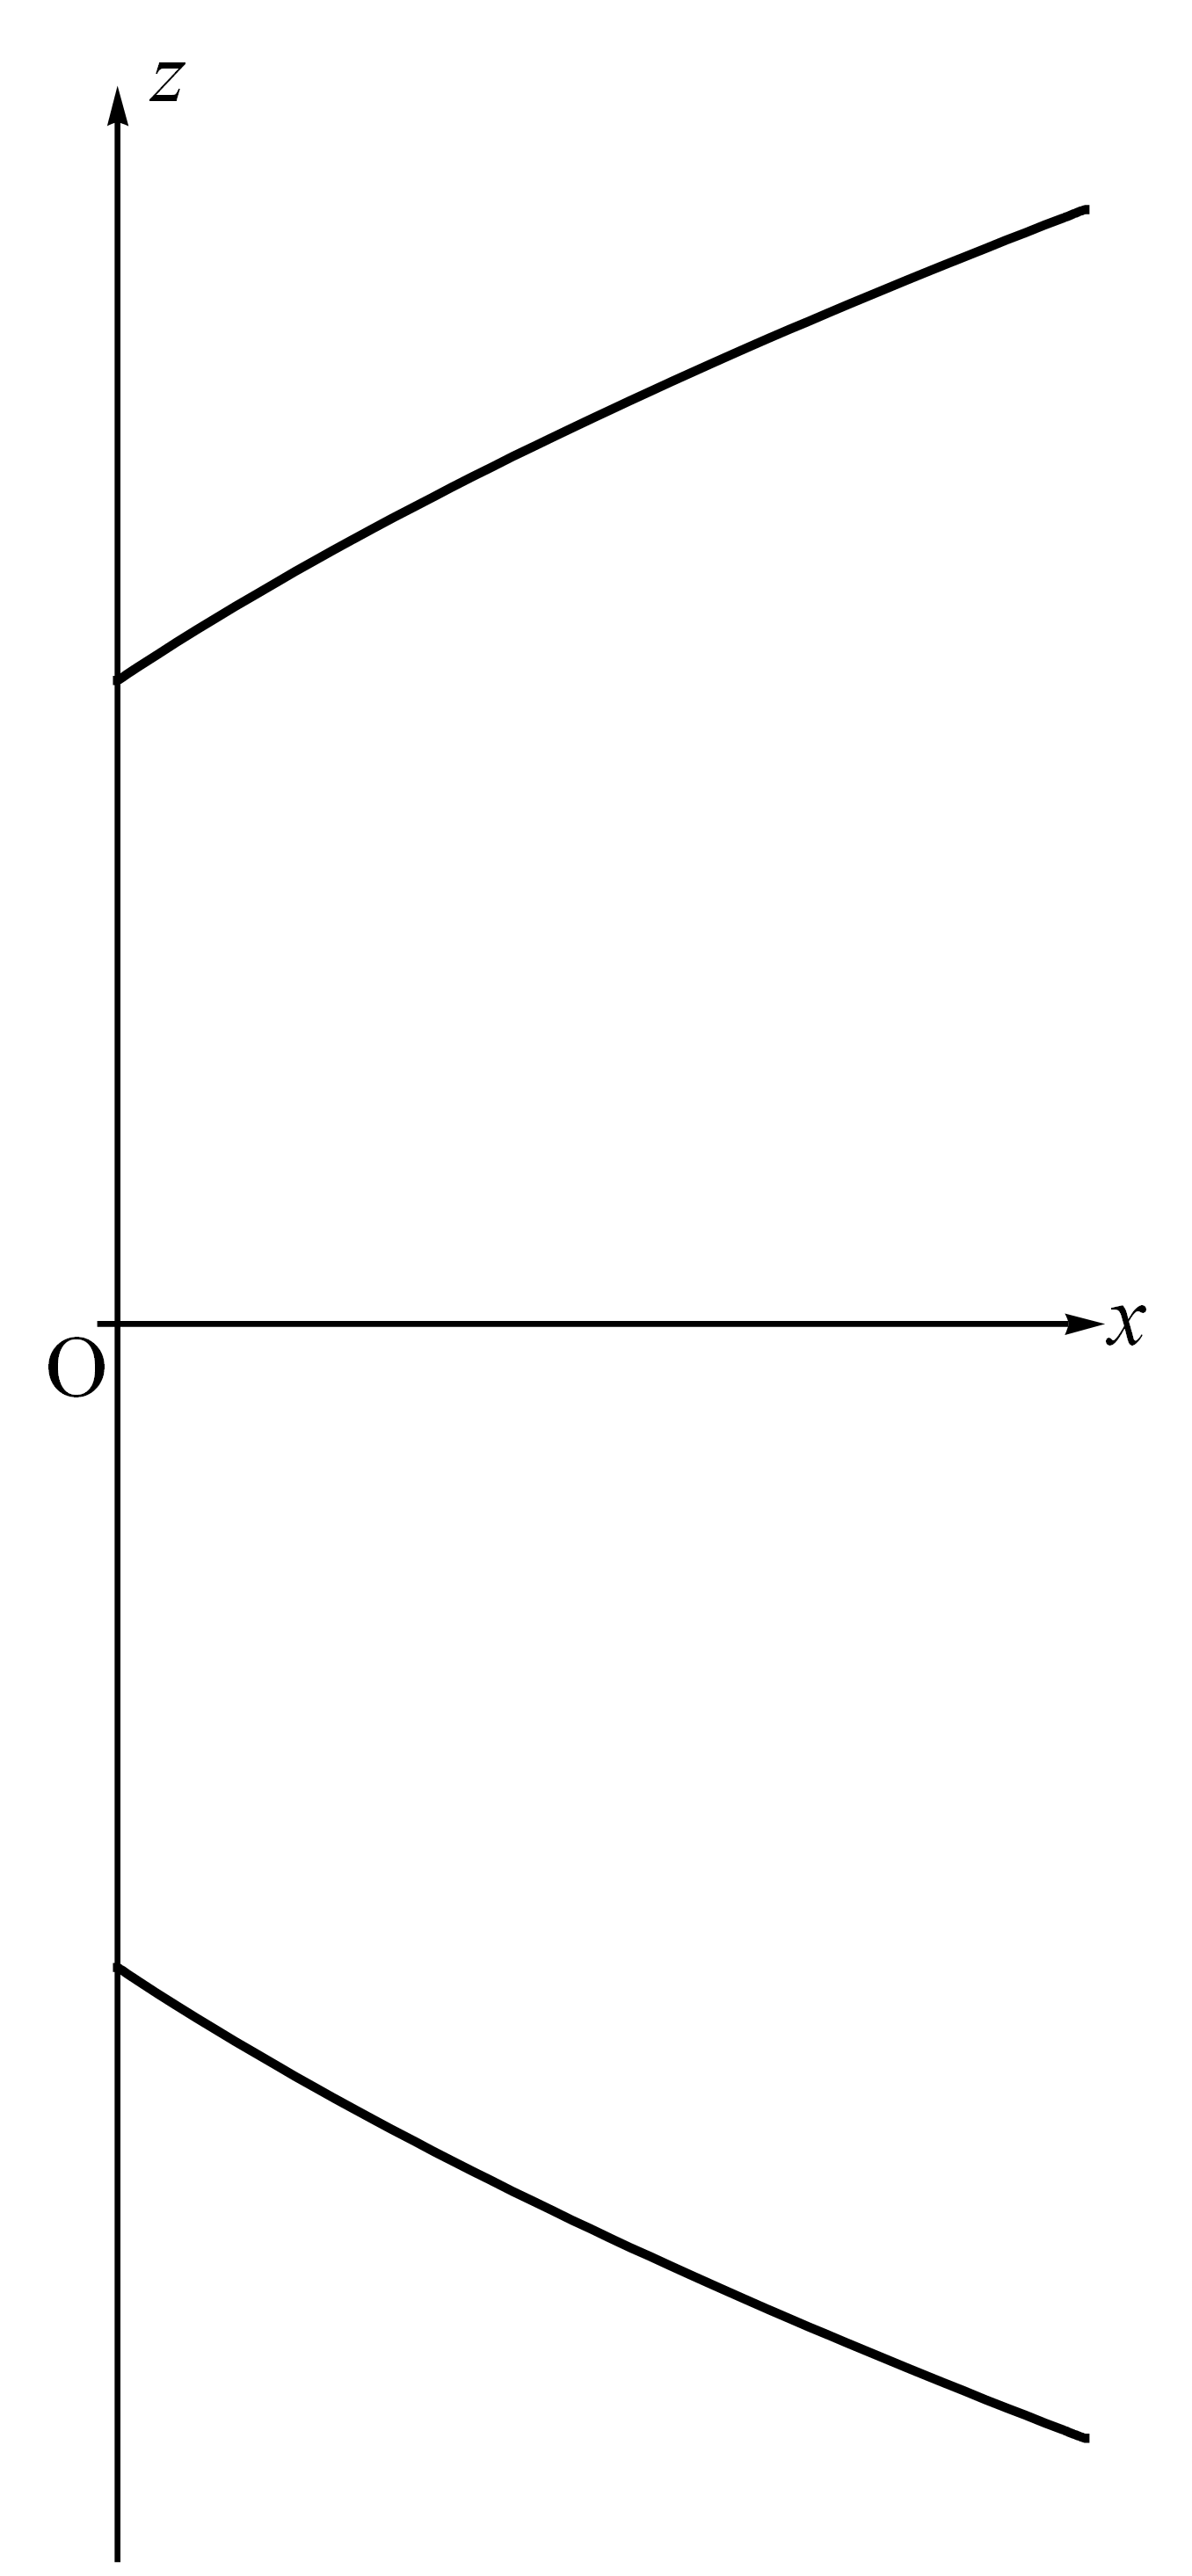
\includegraphics[height=0.3\textheight]{F:/life/2018AutumnTA/Exercises/11/Fig5-7-1-1.png} }}
    \subfloat[]{\label{5-7-1-2} {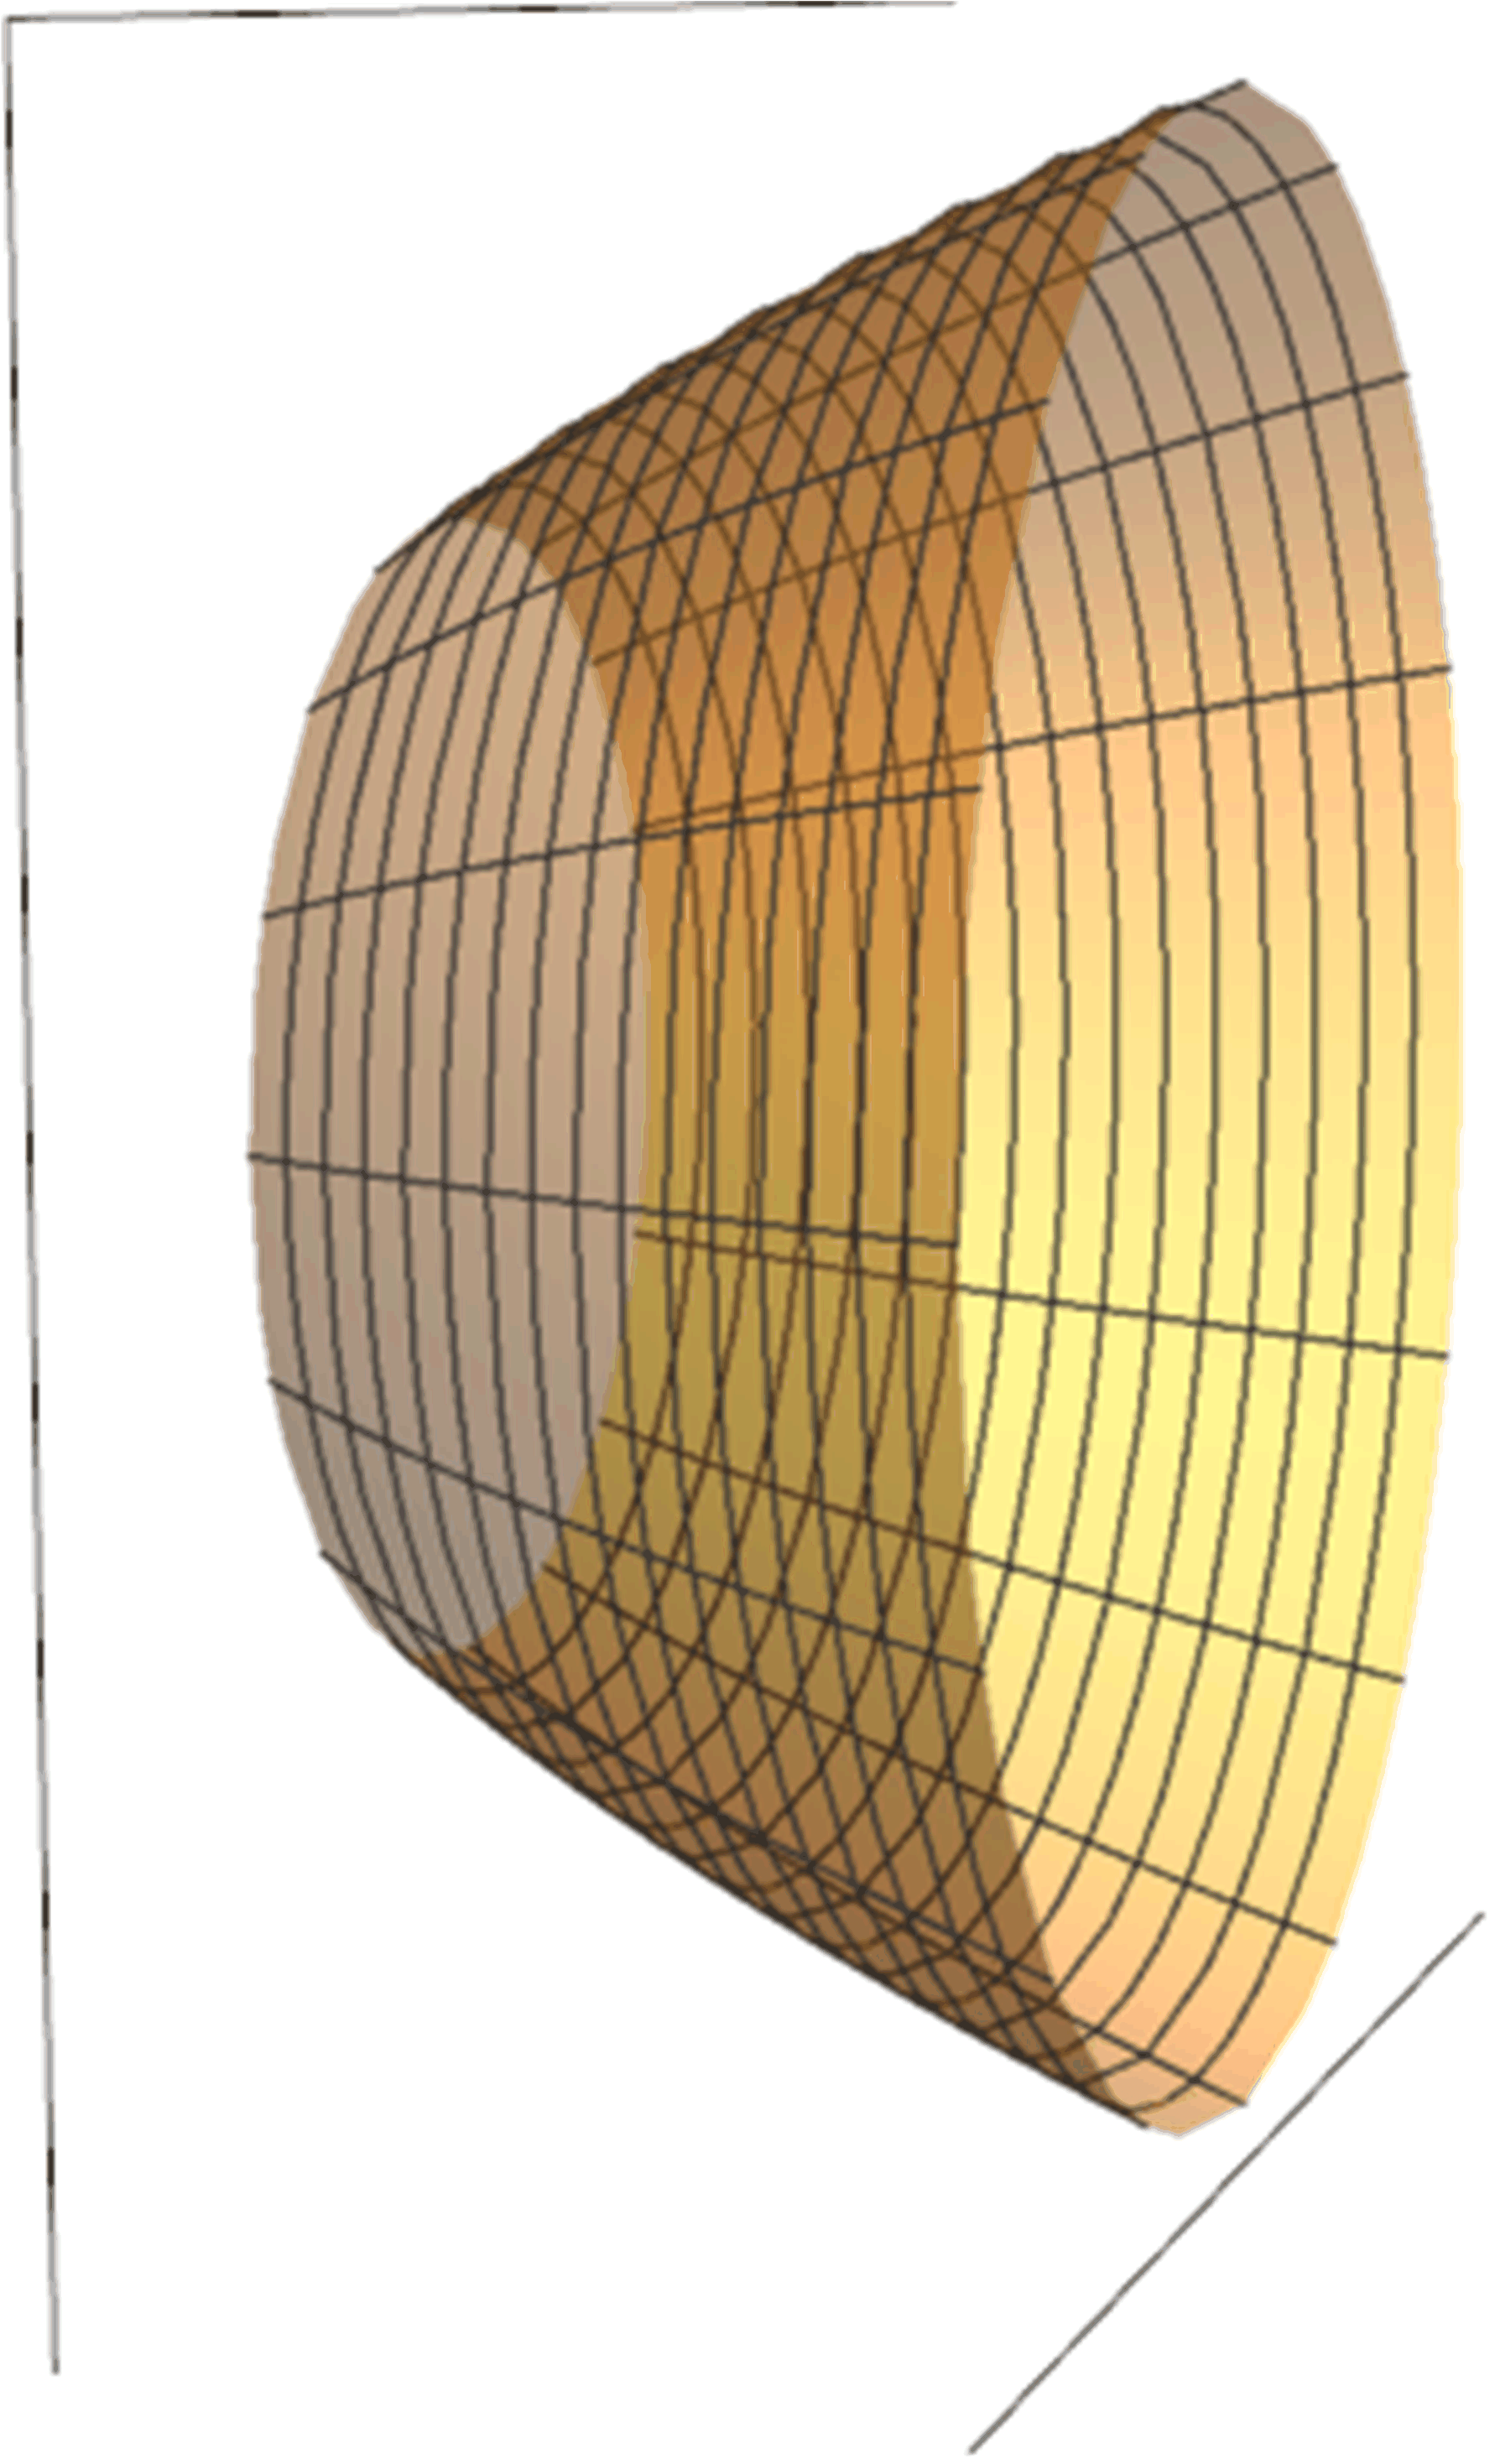
\includegraphics[height=0.3\textheight]{F:/life/2018AutumnTA/Exercises/11/Fig5-7-1-2.png} }}
    \subfloat[]{\label{5-7-1-3} {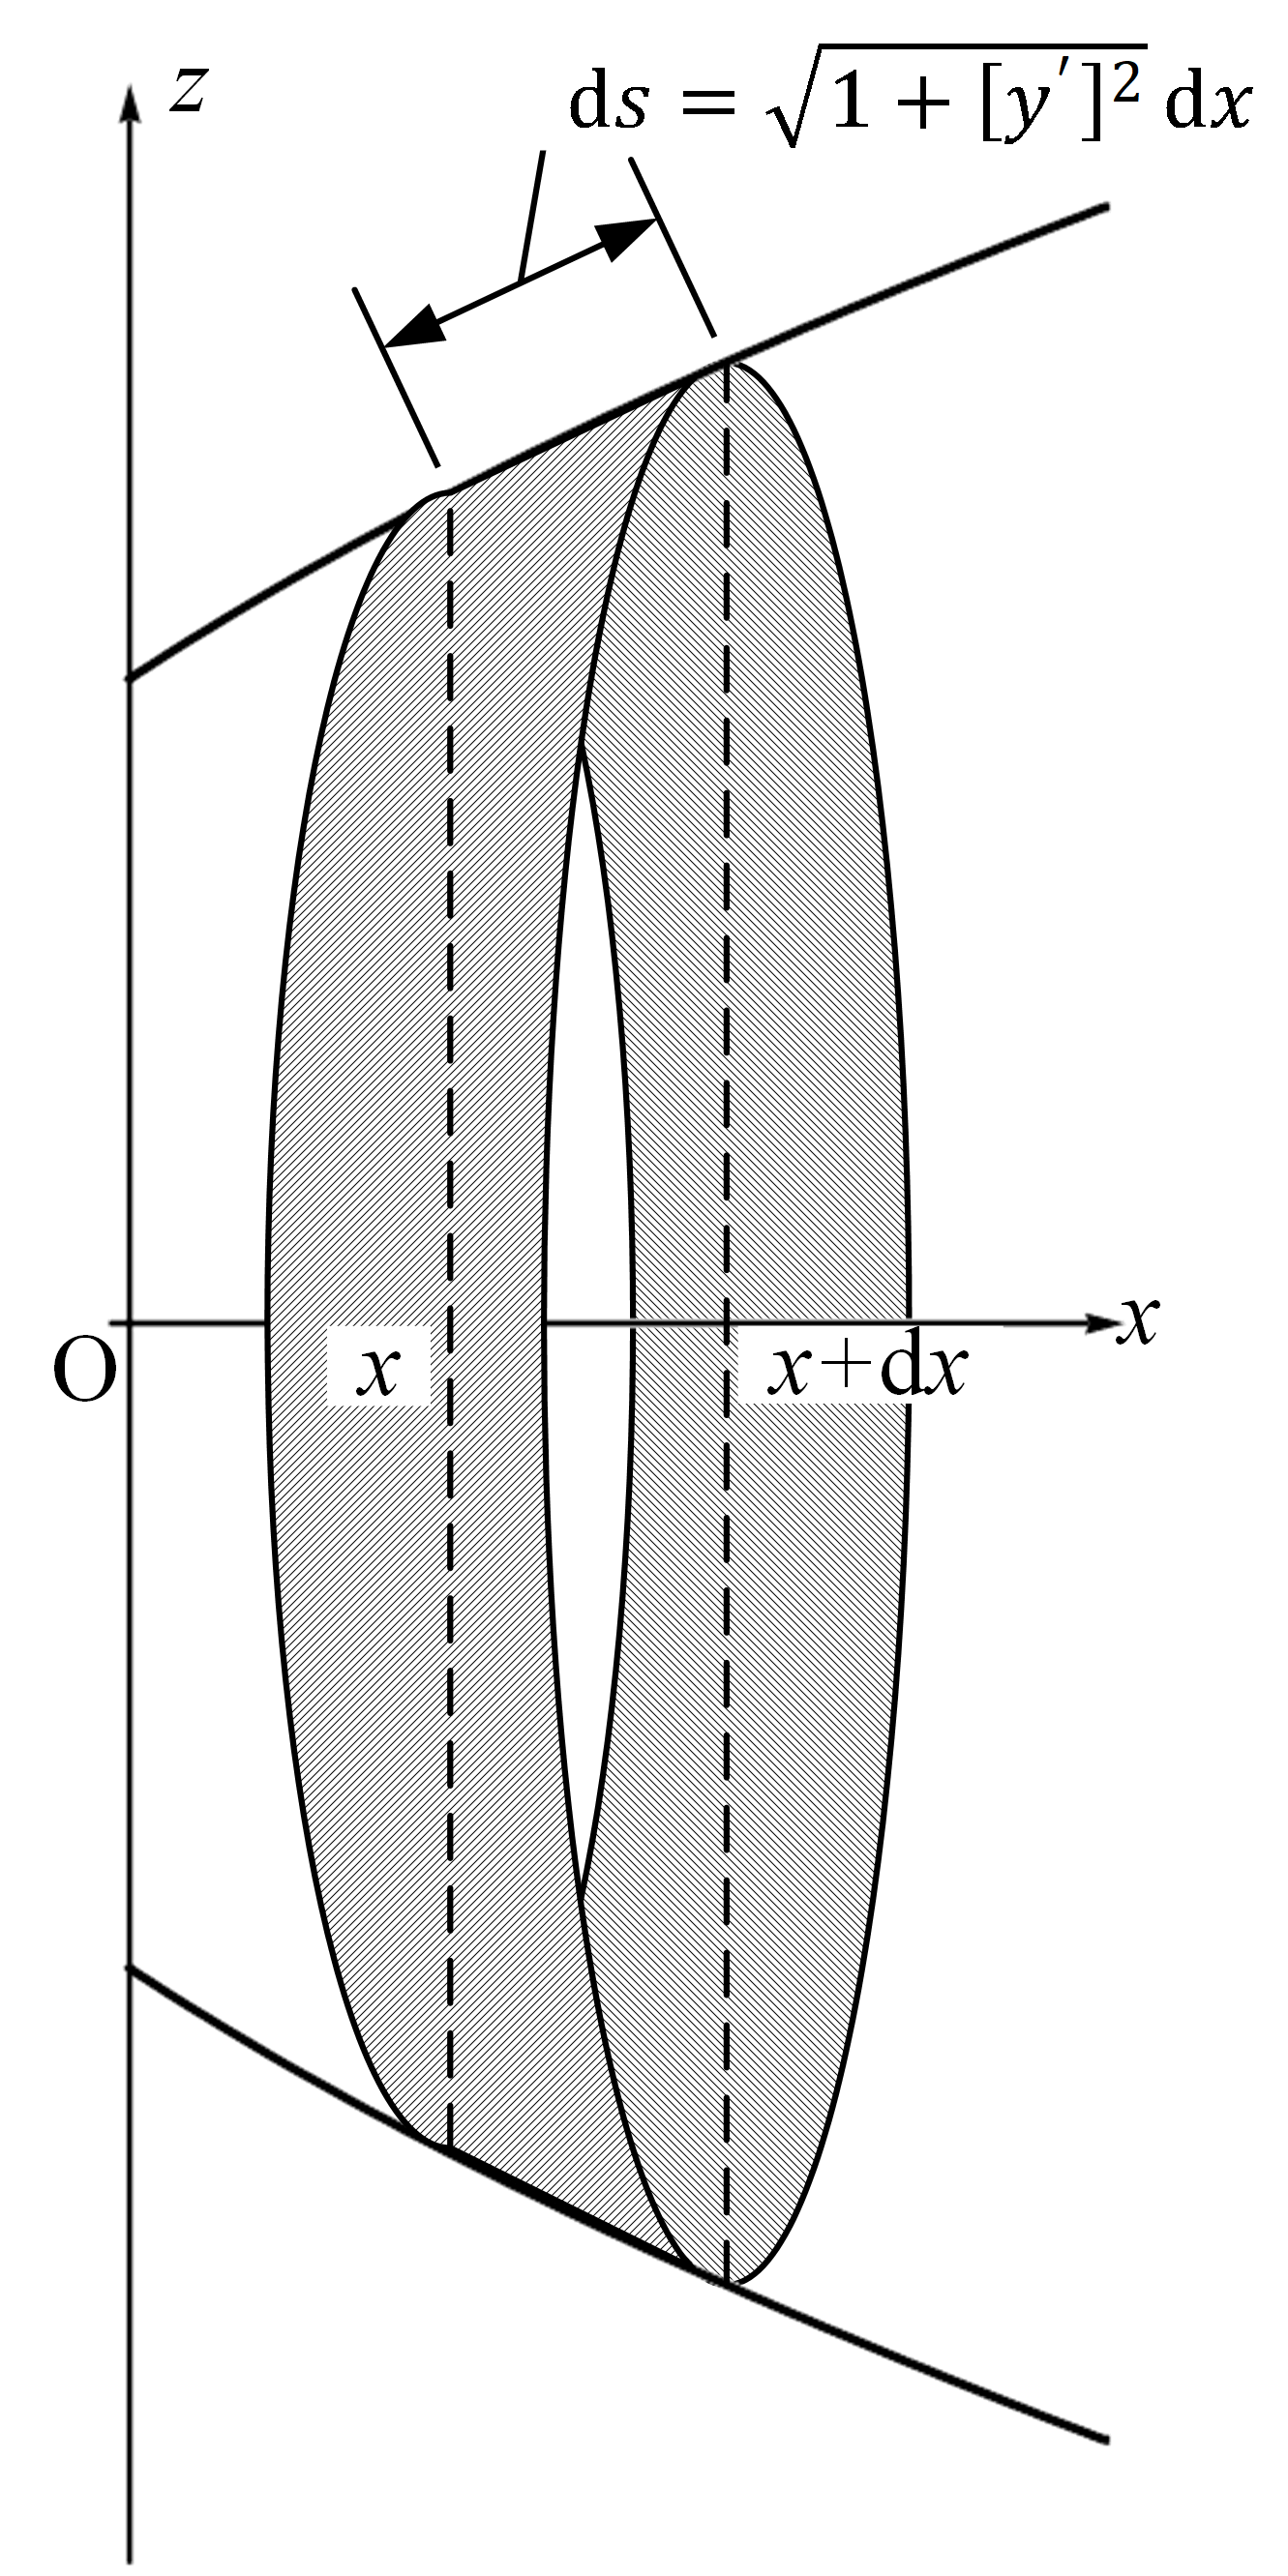
\includegraphics[height=0.3\textheight]{F:/life/2018AutumnTA/Exercises/11/Fig5-7-1-3.png} }}
\end{center}
\caption{7.(1)题图示}
\label{5-7-1}
\end{figure}
取如图~\ref{5-7-1-3}所示的曲面元,当$y>0$时,将$y^2=2px+a$两侧对$x$求导得$2yy'=2p,y'=\frac py$,则该旋转曲面的面积
\[\begin{split}
S&=\int_0^a2\pi y(x)\sqrt{1+[y'(x)]^2}\mathrm dx=\int_0^a2\pi y\sqrt{1+(\frac py)^2}\mathrm dx=2\pi\int_0^a\sqrt{y^2+p^2}\mathrm dx\\
&=2\int_0^a\sqrt{2px+a+p^2}\mathrm dx=\frac{2\pi}{2p}\frac23(2px+a+p^2)^{\frac32}\Big|_0^a\\
&=\frac{2\pi}{3p}(2pa+a+p^2)^{\frac32}-\frac{2\pi}{3p}(a+p^2)^{\frac32}.
\end{split}\]

(2)该旋转曲面的形状如图~\ref{5-7-2-2}所示,
\begin{figure}[H]
\begin{center}
\subfloat[]{\label{5-7-2-1}
{\includegraphics[height=0.15\textheight]{F:/life/2018AutumnTA/Exercises/11/Fig5-7-2-1.png} }}
    \subfloat[]{\label{5-7-2-2} {\includegraphics[height=0.25\textheight]{F:/life/2018AutumnTA/Exercises/11/Fig5-7-2-2.png} }}\\
    \subfloat[]{\label{5-7-2-3} {\includegraphics[height=0.25\textheight]{F:/life/2018AutumnTA/Exercises/11/Fig5-7-2-3.png} }}
\end{center}
\caption{7.(2)题图示}
\label{5-7-2}
\end{figure}
取曲面元如图~\ref{5-7-2-3}所示,当$0\leq t\leq 2\pi$时$x\geq0,y\geq0$,曲面面积
\[\begin{split}
S&=\int_0^{2\pi}2\pi y(t)\sqrt{[x'(t)]^2[(y'(t)]^2}\mathrm dt=\int_0^{2\pi}2\pi a(1-\cos t)\sqrt{a^2(1-\cos t)^2+a^2(\sin t)^2}\mathrm dt\\
&=2\pi a^2\int_0^{2\pi}(1-\cos t)\sqrt{2-2\cos t}\mathrm dt=2\sqrt2\pi a^2\int_0^{2\pi}2\sin^2\frac t2|\sqrt2\sin\frac t2|\mathrm dt\\
&=8\pi a^2\int_0^{2\pi}\sin^3\frac t2\mathrm dt=-16\pi a^2\int_0^{2\pi}(1-\cos^2\frac t2)\mathrm d\cos\frac t2=-16\pi a^2(\cos\frac t2-\frac13\cos^3\frac t2)\Big|_0^{2\pi}\\
&=-16\pi a^2[(-1-1)-\frac13(-1-1)]=\frac{64}3\pi a^2.
\end{split}\]
\end{enumerate}
\subsection{习题7.6解答}
\begin{enumerate}
\item半径等于$r$的球沉入水中,与水面相切. 球体的质量密度与水相同. 现将球从水中取出,外力需要做多少功?

解:建立如图~\ref{7-6-1}所示的坐标系,因球体的质量密度与水相同,故图中的微元在水下提升过程中受到的重力和浮力平衡,将球从水中取出,只在水上提升的过程中克服微元的重力做功,外力做的总功
\[\begin{split}
W=&\int_{-r}^r(r+x)\rho\mathrm g\pi(r^2-x^2)\mathrm dx=\rho\mathrm g\pi\int_{-r}^r(r^3-rx^2+r^2x-x^3)\mathrm dx\\
=&\rho\mathrm g\pi(r^3x-\frac r3x^3+\frac{r^2}2x^2-\frac14x^4)\Big|_{-r}^r=\rho\mathrm g\pi[r^3(2r)-\frac r3(2r^3)+0+0]\\
=&\frac43\rho\mathrm g\pi r^4=\frac43\pi r^4(\text{取}\rho\mathrm g=1).
\end{split}\]

\begin{figure}[H]
\begin{center}
\includegraphics[height=0.3\textheight]{F:/life/2018AutumnTA/Exercises/11/Fig7-6-1.png}
\end{center}
\caption{习题7.6 1.题图示}
\label{7-6-1}
\end{figure}
\item边长等于$1\mathrm m$的质量均匀正立方体,比重为$0.1\mathrm{t/m^3}$. 将其全部压入水中,需要做多少功.

解:方法1:如图~\ref{7-6-2-1}所示,设最初正方体浸入水中部分的深度为$h$,由$\rho_{\text{水}}\mathrm ghL^2=\rho_{\text{正方体}}\mathrm gL^3$得\\
\[h=\frac{\rho_{\text{正方体}}L}{\rho_{\text{水}}}=\frac1{10}L\]
\begin{figure}[H]
\begin{center}
\subfloat[]{\label{7-6-2-1}
{\includegraphics[height=0.3\textheight]{F:/life/2018AutumnTA/Exercises/11/Fig7-6-2-1.png} }}
    \subfloat[]{\label{7-6-2-2} {\includegraphics[height=0.3\textheight]{F:/life/2018AutumnTA/Exercises/11/Fig7-6-2-2.png} }}
\end{center}
\caption{习题7.6 2.题图示}
\label{7-6-2}
\end{figure}
可据此将该正方体分为水上部分$A$和水下部分$B$,水上部分$A$处的微元压入水中需做的功
\[\mathrm dW_A=-\rho_{\text{立方体}}\mathrm gL^2\mathrm dx\cdot(L-h)+\rho_{\text{水}}\mathrm gL^2\mathrm dx\cdot(L-h-x)=[-\rho_{\text{立方体}}(L-h)+\rho_{\text{水}}(L-h-x)]\mathrm gL^2\mathrm dx\]
水下部分$B$处的微元压入水中需做的功
\[\mathrm dW_B=-\rho_{\text{立方体}}\mathrm gL^2\mathrm dx\cdot(L-h)+\rho_{\text{水}}\mathrm gL^2\mathrm dx\cdot(L-h)=(-\rho_{\text{立方体}}+\rho_{\text{水}})\mathrm gL^2(L-h)\mathrm dx\]
则将该正方体全部压入水中需要做的功
\[\begin{split}
W&=W_A+W_B=\int_0^{W_A}\mathrm dW_A+\int_0^{W_B}\mathrm dW_B\\
&=\int_0^{L-h}[-\rho_{\text{立方体}}(L-h)+\rho_{\text{水}}(L-h-x)]\mathrm gL^2\mathrm dx+\int_{-h}^0(-\rho_{\text{立方体}}+\rho_{\text{水}})\mathrm gL^2(L-h)\mathrm dx\\
&=\mathrm gL^2[-\rho_{\text{立方体}}(L-h)x+\rho_{\text{水}}(L-h)x-\rho_{\text{水}}\frac12x^2]\Big|_0^{L-h}+(-\rho_{\text{立方体}}+\rho_{\text{水}})\mathrm gL^2(L-h)x\Big|_{-h}^0\\
&=\mathrm gL^2[-\rho_{\text{立方体}}(L-h)^2+\rho_{\text{水}}(L-h)^2-\rho_{\text{水}}\frac12(L-h)^2]+(-\rho_{\text{立方体}}+\rho_{\text{水}})\mathrm gL^2(L-h)h\\
&=\mathrm gL^2(L-h)^2[-\rho_{\text{立方体}}+\rho_{\text{水}}-\frac12\rho_{\text{水}}]+(-\rho_{\text{立方体}}+\rho_{\text{水}})\mathrm gL^2(L-h)h\\
&=\mathrm gL^2(L-h)^2\frac25\rho_{\text{水}}+\frac9{10}\rho_{\text{水}}\mathrm gL^2(L-h)h\\
&=\mathrm gL^2\rho_{\text{水}}[\frac25(L-h)^2+\frac9{10}(L-h)h]\\
&=\mathrm gL^4\rho_{\text{水}}[\frac25(\frac9{10})^2+\frac9{10}\frac9{10}\frac1{10}]\\
&=405\mathrm g(\mathrm J).
\end{split}\]

方法2:如图~\ref{7-6-2-2}所示的微元压入水中需做的功为
\[\mathrm dW=-\rho_{\text{立方体}}\mathrm g\L^2\mathrm dx\cdot L+\rho_{\text{水}}\mathrm gL^2\mathrm dx\cdot(L-x)=[-\rho_{\text{立方体}}L+\rho_{\text{水}}(L-x)]\mathrm g\L^2\mathrm dx\]
设最初正方体下底与水面相平,最初正方体仅在重力的作用下下沉,设稳定后浸入水中部分$D$的深度为$h$,由$\rho_{\text{水}}\mathrm ghL^2=\rho_{\text{正方体}}\mathrm gL^3$得\\
\[h=\frac{\rho_{\text{正方体}}L}{\rho_{\text{水}}}=\frac1{10}L\]
正方体下沉到浸没深度为$h$的过程中外力不做功,相当于将图中立方体的$C$部分转移到$D$部分的过程中外力不做功,外力只对剩余部分做功,故将该正方体全部压入水中需要做的外力功为
\[\begin{split}
W&=\int_0^W\mathrm dW=\int_0^{L-h}[-\rho_{\text{立方体}}L+\rho_{\text{水}}(L-x)]\mathrm g\L^2\mathrm dx\\
&=\mathrm gL^2[-\rho_{\text{立方体}}Lx+\rho_{\text{水}}(Lx-\frac12x^2)]\Big|_0^{L-h}\\
&=\mathrm gL^2[-\rho_{\text{立方体}}L(L-h)+\rho_{\text{水}}L(L-h)-\frac12\rho_{\text{水}}(L-h)^2]\\
&=\mathrm gL^2(L-h)[-\rho_{\text{立方体}}L+\rho_{\text{水}}L-\frac12\rho_{\text{水}}(L-h)]\\
&=\mathrm gL^2\frac9{10}L[-\frac1{10}\rho_{\text{水}}L+\rho_{\text{水}}L-\frac12\rho_{\text{水}}\frac9{10}L]\\
&=\mathrm g\rho_{\text{水}}L^4\frac9{10}\frac9{20}\\
&=405\mathrm g(\mathrm J).
\end{split}\]

\item水库的闸门是等腰梯形,上底$6\mathrm m$,下底$4\mathrm m$,高$10\mathrm m$. 当上底与水面相齐时,求闸门所受的压力.

解:建立如图~\ref{7-6-3}所示的坐标系,图中微元的长度为
\[L=6-2x\tan\theta=6-2x\frac{\frac{6-4}2}{10}=6-\frac15x\]
微元受到的静水压力
\[\mathrm dP=\rho\mathrm gxL\mathrm dx\]
整个闸门受到的静水压力
\[\begin{split}
P&=\int_0^P\mathrm dP=\int_0^{10}\rho\mathrm gxL\mathrm dx=\int_0^{10}\rho\mathrm gx(6-\frac15x)\mathrm dx=\rho\mathrm g(3x^2-\frac1{15}x^3)\Big|_0^{10}=\frac{700}3(\rho\mathrm g=1).
\end{split}\]
\begin{figure}[H]
\begin{center}
\includegraphics[height=0.3\textheight]{F:/life/2018AutumnTA/Exercises/11/Fig7-6-3.png}
\end{center}
\caption{习题7.6 3.题图示}
\label{7-6-3}
\end{figure}
\item圆形水池直径$20\mathrm m$,高$30\mathrm m$,水深$27\mathrm m$. 如果将水全部抽出,外力要做多少功?

解:建立如图~\ref{7-6-4}所示的坐标系,将图中微元抽出需克服重力做功
\[\mathrm dW=\rho\mathrm g\pi\cdot(\frac{20}2)^2\mathrm dx(30-x)=100\rho\mathrm g\pi(30-x)\mathrm dx\]
外力做的总功
\[W=\int_0^W\mathrm dW=\int_0^{27}100\rho\mathrm g\pi(30-x)\mathrm dx=100\rho\mathrm g\pi(30x-\frac12x^2)\Big|_0^{27}=44550\pi\rho\mathrm g(\mathrm J).\]
\begin{figure}[H]
\begin{center}
\includegraphics[height=0.3\textheight]{F:/life/2018AutumnTA/Exercises/11/Fig7-6-4.png}
\end{center}
\caption{习题7.6 4.题图示}
\label{7-6-4}
\end{figure}
\item有一个质量为$M$、半径等于$R$的均匀圆周. 在过圆心、且与圆所在平面垂直的直线上距离圆心等于$h$处有一个质量等于$m$的质点. 求圆周对于质点的引力.

解:如图~\ref{7-6-5}所示,取图中所示的质量元,其与关于圆心中心对称的质量元对质点的合力指向圆心,二者对质点在圆周所在平面内的分力$\mathrm dF_x$互相抵消,只需考虑每个质量元对质点指向圆心的分力
\[\mathrm dF_y=\frac{Gm\mathrm dM}{R^2+h^2}\cos\theta=\frac{Gm}{R^2+h^2}\frac h{\sqrt{R^2+h^2}}\mathrm dM\]
整个圆周对质点的引力
\[F=\int_0^F\mathrm dF=\int_0^M\frac{Gm}{R^2+h^2}\frac h{\sqrt{R^2+h^2}}\mathrm dM=\frac{GmMh}{(R^2+h^2)^{\frac32}}=\frac{Mmh}{(R^2+h^2)^{\frac32}}(G=1).\]
\begin{figure}[H]
\begin{center}
\includegraphics[height=0.3\textheight]{F:/life/2018AutumnTA/Exercises/11/Fig7-6-5.png}
\end{center}
\caption{习题7.6 5.题图示}
\label{7-6-5}
\end{figure}
\item设$2\mathrm{kg}$的力能使弹簧伸长$1\mathrm{cm}$. 求使弹簧伸长$1\mathrm m$需要做的功.

解:弹簧常数$k=\frac{m\mathrm g}{\Delta x}=\frac{2\mathrm g}{0.01}=200\mathrm g$

使弹簧伸长$1\mathrm m$需要做功$W=\int_0^1kx\mathrm dx=\frac12kx^2\Big|_0^1=\frac12\times200\mathrm g=100\mathrm g(\mathrm J).$
\end{enumerate}
\subsection{习题7.7解答}
\begin{enumerate}
\item计算下列反常积分:
\newline
\begin{tabular}{ll}
(1)$\int_2^{+\infty}\frac{\mathrm dx}{x^2-1}$;&(2)$\int_1^{+\infty}\frac{\arctan x}{x^3}\mathrm dx$;\\
(3)$\int_0^{+\infty}x\mathrm e^{-x^2}\mathrm dx$;&(4)$\int_{\mathrm e}^{+\infty}\frac{\mathrm dx}{x(\ln x)^2}$;\\
(5)$\int_1^{+\infty}\frac{\mathrm dx}{x\sqrt{x^2-1}}$;&(6)$\int_0^1\frac{\arcsin x}{\sqrt{1-x^2}}\mathrm dx$;\\
(7)$\int_0^1\ln x\mathrm dx$;&(8)$\int_1^{\mathrm e}\frac{\mathrm dx}{x\sqrt{1-(\ln x)^2}}$.
\end{tabular}

解:(1)$\int_2^{+\infty}\frac{\mathrm dx}{x^2-1}=\frac12\int_2^{+\infty}(\frac1{x-1}-\frac1{x+1})=\frac12\ln|\frac{x-1}{x+1}|\Big|_2^{+\infty}=-\frac12\ln\frac13=\frac12\ln3$.

(2)$\int_1^{+\infty}\frac{\arctan x}{x^3}\mathrm dx=\int_1^{+\infty}\arctan x\mathrm d(-\frac1{2x^2})=-\frac{\arctan x}{x^2}\Big|_1^{+\infty}+\int_1^{+\infty}\frac1{x^2}\mathrm d\arctan x\\
=\frac\pi4+\int_1^{+\infty}\frac1{x^2(1+x^2)}\mathrm dx=-\frac\pi4+\int_1^{+\infty}(\frac1{x^2}-\frac1{1+x^2})\mathrm dx=\frac\pi4+(-\frac1x-\arctan x)\Big|_1^{+\infty}\\
=\frac\pi4+[1-(\frac\pi2-\frac\pi4)]=1$.

(3)$\int_0^{+\infty}x\mathrm e^{-x^2}\mathrm dx=-\frac12\int_0^{+\infty}\mathrm e^{-x^2}\mathrm d(-x^2)=\mathrm e^{-x^2}\Big|_0^{+\infty}=-1$.

(4)$\int_{\mathrm e}^{+\infty}\frac{\mathrm dx}{x(\ln x)^2}=\int_{\mathrm e}^{+\infty}\frac1{(\ln x)^2}\mathrm d\ln x=-\frac1{\ln x}\Big|_{\mathrm e}^{+\infty}=1$.

(5)$\int_1^{+\infty}\frac{\mathrm dx}{x\sqrt{x^2-1}}\xlongequal{x=\sec t}\int_0^{\frac\pi2}\frac{\sec t\tan t\mathrm dt}{\sec t\tan t}=\frac\pi2$.

(6)$\int_0^1\frac{\arcsin x}{\sqrt{1-x^2}}\mathrm dx=\int_0^1\arcsin x\mathrm d\arcsin x=\frac12\arcsin^2x\Big|_0^1=\frac{\pi^2}8$.

(7)$\int_0^1\ln x\mathrm dx=x\ln x\Big|_0^1-\int_0^1x\mathrm d\ln x=-\int_0^1x\frac1x\mathrm dx=-1$.

(8)$\int_1^{\mathrm e}\frac{\mathrm dx}{x\sqrt{1-(\ln x)^2}}=\int_1^{\mathrm e}\frac{\mathrm d\ln x}{\sqrt{1-(\ln x)^2}}=\arcsin(\ln x)\Big|_1^{\mathrm e}=\frac\pi2$.
\item讨论下列广义积分的收敛性:
\newline
\begin{tabular}{ll}
(1)$\int_0^{+\infty}\frac{x^2}{x^4-x^2+1}\mathrm dx$;&(2)$\int_0^{+\infty}\frac{x^m}{1+x^n}\mathrm dx,m>0,n>0$;\\
(3)$\int_0^{+\infty}x^n\mathrm e^{-x}\mathrm dx,n>0$;&(4)$\int_1^{+\infty}\frac{\mathrm dx}{x^p+x^q},p>0,q>0$;\\
(5)$\int_0^1x^a\ln x\mathrm dx,a>0$;&(6)$\int_0^1\frac{\ln x}{1-x}\mathrm dx$;\\
\multicolumn{2}{l}{(7)$\int_0^{\frac\pi2}\frac{\mathrm dx}{\sin^px\cos^qx},p>0,q>0$;}\\
\multicolumn{2}{l}{(8)$\int_0^1x^{p-1}(1-x)^{q-1}\ln x\mathrm dx$.}
\end{tabular}

解:(1)$\because\lim\limits_{x\rightarrow+\infty}x^2\cdot\frac{x^2}{x^4-x^3+1}=1$

$\therefore\int_0^{+\infty}\frac{x^2}{x^4-x^2+1}\mathrm dx$收敛.

(2)$\because\lim\limits_{x\rightarrow+\infty}x^{n-m}\cdot\frac{x^m}{1+x^n}=\lim\limits_{x\rightarrow+\infty}\frac{x^n}{1+x^n}=1$

$\therefore$当$n-m>1$时,$\int_0^{+\infty}\frac{x^m}{1+x^n}\mathrm dx$收敛,当$n-m\leq1$时$\int_0^{+\infty}\frac{x^m}{1+x^n}\mathrm dx$发散.

(3)$\because\lim\limits_{x\rightarrow+\infty}x^2\cdot x^n\mathrm e^{-x}=\lim\limits_{x\rightarrow+\infty}\frac{x^{n+2}}{\mathrm e^x}=0$

$\therefore\int_0^{+\infty}x^n\mathrm e^{-x}\mathrm dx$收敛.

(4)不妨设$p\geq q$,$\lim\limits_{x\rightarrow+\infty}x^p\cdot\frac1{x^p+x^q}=\begin{cases}
1,&p>q\\
\frac12,&p=q
\end{cases}$

i)当$p>1$或$q>1$时,$\int_1^{+\infty}\frac{\mathrm dx}{x^p+x^q}$收敛;

ii)当$p\leq1$且$q\leq1$时,$\int_1^{+\infty}\frac{\mathrm dx}{x^p+x^q}$发散.

(5)$\because\lim\limits_{x\rightarrow0^+}x^{\frac12}\cdot|x^a\ln x|=-\lim\limits_{x\rightarrow0^+}x^{\frac12+a}\ln x=0$

$\therefore\int_0^1x^a\ln x\mathrm dx$收敛.

(6)$\int_0^1\frac{\ln x}{1-x}\mathrm dx=\int_0^{\frac12}\frac{\ln x}{1-x}\mathrm dx+\int_{\frac12}^1\frac{\ln x}{1-x}\mathrm dx=I_1+I_2$

$\because\lim\limits_{x\rightarrow0^+}x^{\frac12}\cdot|\frac{\ln x}{1-x}|=-\lim\limits_{x\rightarrow0^+}x^{\frac12}\cdot\frac{\ln x}{1-x}=0$,故$I_1$收敛;

$\because\lim\limits_{x\rightarrow1^-}(1-x)^{\frac12}\cdot|\frac{\ln x}{1-x}|=-\lim\limits_{x\rightarrow1^-}(1-x)^{\frac12}\cdot\frac{\ln[1-(1-x)]}{1-x}=-\lim\limits_{x\rightarrow1^-}(1-x)^{\frac12}\cdot(-1)=0$,故$I_2$收敛;

综上所述,$\int_0^1\frac{\ln x}{1-x}\mathrm dx$收敛.

(7)$\int_0^{\frac\pi2}\frac{\mathrm dx}{\sin^px\cos^qx}=\int_0^{\frac\pi4}\frac{\mathrm dx}{\sin^px\cos^qx}+\int_{\frac\pi4}^{\frac\pi2}\frac{\mathrm dx}{\sin^px\cos^qx}=I_1+I_2$

$\because\lim\limits_{x\rightarrow0^+}x^p\cdot\frac1{\sin^px\cos^qx}=\frac{x^p}{\sin^px}\frac1{\cos^qx}=1$

$\therefore$当$p<1$时$I_1$收敛,当$p\geq1$时$I_1$发散;

$\because\lim\limits_{x\rightarrow\frac\pi2^-}(\frac\pi2-x)^q\cdot\frac1{\sin^px\cos^qx}=\lim\limits_{x\rightarrow\frac\pi2^-}\frac1{\sin^px}\frac{(\frac\pi2-x)^q}{\sin^q(\frac\pi2-x)}=1$

$\therefore$当$q<1$时$I_2$收敛,当$q\geq1$时$I_2$发散;

综上所述,当$p<1$且$q<1$时$\int_0^{\frac\pi2}\frac{\mathrm dx}{\sin^px\cos^qx}$收敛,否则发散.

(8)$\int_0^1x^{p-1}(1-x)^{q-1}\ln x\mathrm dx=\int_0^{\frac12}x^{p-1}(1-x)^{q-1}\ln x\mathrm dx+\int_{\frac12}^1x^{p-1}(1-x)^{q-1}\ln x\mathrm dx=I_1+I_2$

i)$\lim\limits_{x\rightarrow0^+}x^a\cdot|x^{p-1}(1-x)^{q-1}\ln x|=-\lim\limits_{x\rightarrow0^+}(1-x)^{q-1}x^{a+p-1}\ln x=\begin{cases}
0,&a+p-1>0\\
+\infty,&a+p-1\leq0
\end{cases}$

\textcircled{1}当$1-p<1$,即$p>0$时,取$a=\frac{1-p+1}2=\frac{2-p}2<1$,则$a+p-1=\frac p2>0$,$I_1$收敛,

\textcircled{2}当$1-p\geq1$,即$p\leq0$时,取$a=\frac{1-p+1}2=\frac{2-p}2\geq1$,则$a+p-1=\frac p2\leq0$,$I_1$发散;

ii)$\lim\limits_{x\rightarrow1^-}(1-x)^b\cdot|x^{p-1}(1-x)^{q-1}\ln x|=-\lim\limits_{x\rightarrow1^-}x^{p-1}(1-x)^{b+q-1}\ln[1-(1-x)]\\
=-\lim\limits_{x\rightarrow1^-}x^{p-1}(1-x)^{b+q-1}[-(1-x)]=\lim\limits_{x\rightarrow1^-}x^{p-1}(1-x)^{b+q}=\begin{cases}
0,&b+q>0\\
1,&b+q=0\\
+\infty,&b+q<0
\end{cases}$

\textcircled{1}当$-q<1$,即$q>-1$时,取$b=\frac{-q+1}2=\frac{1-q}2<1$,则$b+q=\frac{q+1}2>0$,$I_2$收敛,

\textcircled{2}当$-q\geq1$,即$q\leq-1$时,取$b=\frac{-q+1}2=\frac{1-q}2\geq1$,则$b+q=\frac{q+1}2\leq0$,$I_2$发散;

综上所述,当$p>0$且$q>-1$时,$\int_0^1x^{p-1}(1-x)^{q-1}\ln x\mathrm dx$收敛,否则发散.

\item设$f(x),g(x)$在任意区间$[0,A]$上可积$(A>0)$,且$\int_0^{+\infty}f^2(x)\mathrm dx,\int_0^{+\infty}g^2(x)\mathrm dx$都收敛,试证:
\newline
(1)$\int_0^{+\infty}f(x)g(x)\mathrm dx$绝对收敛,即$\int_0^{+\infty}|f(x)g(x)|\mathrm dx$收敛;
\newline
(2)$\int_0^{+\infty}(f(x)+g(x))^2\mathrm dx$收敛.

证明:(1)$\because0\leq|f(x)g(x)|\leq\frac{f^2(x)+g^2(x)}2,x\in[0,A],A>0$

又$\because\int_0^{+\infty}f^2(x)\mathrm dx,\int_0^{+\infty}g^2(x)\mathrm dx$都收敛

$\therefore\int_0^{+\infty}\frac{f^2(x)+g^2(x)}2\mathrm dx$收敛

$\therefore\int_0^{+\infty}|f(x)g(x)|\mathrm dx$收敛

$\therefore\int_0^{+\infty}f(x)g(x)\mathrm dx$绝对收敛.

(2)$\because\int_0^{+\infty}f(x)g(x)\mathrm dx$绝对收敛

$\therefore\int_0^{+\infty}f(x)g(x)\mathrm dx$收敛

$\therefore\int_0^{+\infty}(f(x)+g(x))^2\mathrm dx=\int_0^{+\infty}(f^2(x)+2f(x)g(x)+g^2(x))\mathrm dx$收敛.
\end{enumerate}
\end{document} 
\documentclass[12pt,UTF8]{ctexart}
\usepackage{ctex,amsmath,amssymb,geometry,fancyhdr,bm,amsfonts
,mathtools,extarrows,graphicx,url,enumerate,color,float,multicol} 
% 加入中文支持
\newcommand\Set[2]{%
\left\{#1\ \middle\vert\ #2 \right\}}
\geometry{a4paper,scale=0.80}
\pagestyle{fancy}
\rhead{第7章补充题}
\lhead{基础习题课讲义}
\chead{微积分B(1)}
\begin{document}
\def\thesection{11C}
\section{第7章补充题}
\def\thesubsection{\thesection.\arabic{subsection}}
\subsection{第7章补充题解答}
\begin{enumerate}
\item设$f\in R[a,b],g\in R[a,b]$,求证:
\[
\Big(\int_a^bf(x)g(x)\mathrm dx\Big)^2\leq\int_a^bf^2(x)\mathrm dx\int_a^bg^2(x)\mathrm dx
\]
证明:令$F(x)=\Big(\int_a^xf(t)g(t)\mathrm dt\Big)^2-\int_a^xf^2(t)\mathrm dt\int_a^xg^2(t)\mathrm dt$

$F'(x)=2\int_a^xf(t)g(t)\mathrm dtf(x)g(x)-f^2(x)\int_a^xg^2(t)\mathrm dt-g^2(x)\int_a^xf^2(t)\mathrm dt\\
=\int_a^x[2f(t)g(t)f(x)g(x)-f^2(x)g^2(t)-g^2(x)f^2(t)]\mathrm dt\\
=-\int_a^x[f(x)g(t)-f(t)g(x)]^2\mathrm dt\leq0$

$\therefore F(x)\leq F(0)=0$,即$\Big(\int_a^bf(x)g(x)\mathrm dx\Big)^2\leq\int_a^bf^2(x)\mathrm dx\int_a^bg^2(x)\mathrm dx$.

\item设$f(x)$在区间$[0,1]$上连续且单调减少,又设$f(x)>0$,求证对于任意满足$0<\alpha<\beta<1$的$\alpha$和$\beta$,有
\[
\beta\int_0^\alpha f(x)\mathrm dx>\alpha\int_0^\beta f(x)\mathrm dx
\]
证明:方法1:令$F(x)=x\int_0^\alpha f(t)\mathrm dt-\alpha\int_0^xf(t)\mathrm dt$

$F'(x)=\int_0^\alpha f(t)\mathrm dt-\alpha f(x),F''(x)=-\alpha f'(x)$

$\because f(x)$在区间$[0,1]$上连续且单调减少

$\therefore F''(x)=-\alpha f'(x)>0$

$\therefore$当$x>\alpha$时$F'(x)=\int_0^\alpha f(t)\mathrm dt-\alpha f(x)>F(\alpha)=\int_0^\alpha f(t)\mathrm dt-\alpha f(\alpha)\\
=\int_0^\alpha[f(t)-f(\alpha)]\mathrm dt>0$

$\therefore$当$x>\alpha$时$F(x)>F(\alpha)=0$

$\therefore$对于任意满足$0<\alpha<\beta<1$的$\alpha$和$\beta$,有$\beta\int_0^\alpha f(x)\mathrm dx>\alpha\int_0^\beta f(x)\mathrm dx$.

方法2:$\beta\int_0^\alpha f(x)\mathrm dx-\alpha\int_0^\beta f(x)\mathrm dx=\beta\int_0^\alpha f(x)\mathrm dx-\alpha\int_0^\alpha f(x)\mathrm dx-\alpha\int_\alpha^\beta f(x)\mathrm dx\\
=(\beta-\alpha)\int_0^\alpha f(x)\mathrm dx-\alpha\int_\alpha^\beta f(x)\mathrm dx=(\beta-\alpha)\alpha f(\xi_1)-\alpha(\beta-\alpha)f(\xi_2)\\
=\alpha(\beta-\alpha)[f(\xi_1)-f(\xi_2)]>0,\xi_1\in(0,\alpha),\xi_2\in(\alpha,\beta)$

$\therefore$对于任意满足$0<\alpha<\beta<1$的$\alpha$和$\beta$,有$\beta\int_0^\alpha f(x)\mathrm dx>\alpha\int_0^\beta f(x)\mathrm dx$.

\item设$f(x),g(x)$在区间$[0,+\infty)$上连续,其中$f(x)>0(0\leq x<+\infty)$,$g(x)$在区间$[0,+\infty)$上单调增加,令
\[
\varphi(x)=\frac{\int_0^xf(t)g(t)\mathrm dt}{\int_0^xf(t)\mathrm dt}.
\]
求证$\varphi(x)$在区间$[0,+\infty)$上单调增加.

证明:$\because f(x)>0(0\leq x<+\infty)$,$g(x)$在区间$[0,+\infty)$上单调增加

$\therefore\varphi'(x)=\frac{f(x)g(x)\int_0^xf(t)\mathrm dt-f(x)\int_0^xf(t)g(t)\mathrm dt}{[\int_0^xf(t)\mathrm dt]^2}=f(x)\frac{\int_0^xf(t)[g(x)-g(t)]\mathrm dt}{[\int_0^xf(t)\mathrm dt]^2}>0,x\in[0,+\infty)$

【或者$\varphi'(x)=\frac{f(x)g(x)\int_0^xf(t)\mathrm dt-f(x)\int_0^xf(t)g(t)\mathrm dt}{[\int_0^xf(t)\mathrm dt]^2}=f(x)\frac{\int_0^xf(t)[g(x)-g(t)]\mathrm dt}{[\int_0^xf(t)\mathrm dt]^2}\\
=f(x)\frac{xf(\xi)[g(x)-g(\xi)]}{[\int_0^xf(t)\mathrm dt]^2}>0,\xi\in(0,x),x\in[0,+\infty)$】

$\therefore\varphi(x)$在区间$[0,+\infty)$上单调增加.
\item设$f'(x)$在区间$[a,b]$上连续,且$f(a)=f(b)=0$,求证:
\[
\Big|\int_a^bf(x)\mathrm dx\Big|\leq\frac{(b-a)^2}4\max\limits_{a\leq x\leq b}|f'(x)|
\]
证明:$\because f'(x)$在区间$[a,b]$上连续,且$f(a)=f(b)=0$

$\therefore f(x)=f'(\xi_1)(x-a),f(x)=f'(\xi_2)(x-b),\xi_1\in(a,x),\xi_2\in(x,b)$

$\therefore\big|\int_a^{\frac{a+b}2}f(x)\mathrm dx\big|=\big|\int_a^{\frac{a+b}2}f'(\xi_1)(x-a)\mathrm dx\big|\leq\int_a^{\frac{a+b}2}\big|f'(\xi_1)\big|(x-a)\mathrm dx\\
\leq\int_a^{\frac{a+b}2}\max\limits_{a\leq x\leq b}\big|f'(x)\big|(x-a)\mathrm dx=\max\limits_{a\leq x\leq b}\big|f'(x)\big|\int_a^{\frac{a+b}2}(x-a)\mathrm dx=\frac18(b-a)^2\max\limits_{a\leq x\leq b}\big|f'(x)\big|$

$\big|\int_{\frac{a+b}2}^bf(x)\mathrm dx\big|=\big|\int_{\frac{a+b}2}^bf'(\xi_2)(x-b)\mathrm dx\big|\leq\int_{\frac{a+b}2}^b\big|f'(x)\big|(b-x)\mathrm dx\\
\leq\int_{\frac{a+b}2}^b\max\limits_{a\leq x\leq b}\big|f'(x)\big|(b-x)\mathrm dx=\max\limits_{a\leq x\leq b}\big|f'(x)\big|\int_{\frac{a+b}2}^b(b-x)\mathrm dx=\frac18(b-a)^2\max\limits_{a\leq x\leq b}\big|f'(x)\big|$

$\therefore\big|\int_a^bf(x)\mathrm dx\big|=\big|\int_a^{\frac{a+b}2}f(x)\mathrm dx+\int_{\frac{a+b}2}^bf(x)\mathrm dx\big|\leq\big|\int_a^{\frac{a+b}2}f(x)\mathrm dx\big|+\big|\int_{\frac{a+b}2}^bf(x)\mathrm dx\big|\\
\leq\frac18(b-a)^2\max\limits_{a\leq x\leq b}\big|f'(x)\big|+\frac18(b-a)^2\max\limits_{a\leq x\leq b}\big|f'(x)\big|=\frac14(b-a)^2\max\limits_{a\leq x\leq b}\big|f'(x)\big|$.

\item设$f(x)$在区间$[a,b]$上连续且单调增加,证明:
\[
\int_a^bxf(x)\mathrm dx\geq\frac{a+b}2\int_a^bf(x)\mathrm dx
\]
证明:$\int_a^b(x-\frac{a+b}2)f(x)\mathrm dx=\int_a^{\frac{a+b}2}(x-\frac{a+b}2)f(x)\mathrm dx+\int_{\frac{a+b}2}^b(x-\frac{a+b}2)f(x)\mathrm dx$

$\because f(x)$在$[a,b]$上连续,$g(x)=x-\frac{a+b}2$在$[a,\frac{a+b}2]$上连续且非正,$g(x)=x-\frac{a+b}2$在$[\frac{a+b}2,b]$上连续且非负

$\therefore\int_a^b(x-\frac{a+b}2)f(x)\mathrm dx=f(\xi_1)\int_a^{\frac{a+b}2}(x-\frac{a+b}2)\mathrm dx+f(\xi_2)\int_{\frac{a+b}2}^b(x-\frac{a+b}2)\mathrm dx\\
=f(\xi_1)(\frac12x^2-\frac{a+b}2x)\Big|_a^{\frac{a+b}2}+f(\xi_2)(\frac12x^2-\frac{a+b}2x)\Big|_{\frac{a+b}2}^b\\
=\frac18(b-a)^2[f(\xi_2)-f(\xi_1)],\xi_2\in(\frac{a+b}2,b),\xi_1\in(a,\frac{a+b}2)$

$\because f(x)$在$[a,b]$上单调增加

$\therefore\int_a^b(x-\frac{a+b}2)f(x)\mathrm dx=\frac18(b-a)^2[f(\xi_2)-f(\xi_1)]>0$,即$\int_a^bxf(x)\mathrm dx\geq\frac{a+b}2\int_a^bf(x)\mathrm dx$.

\item设$f(x)$在区间$[0,1]$上连续,下凸且非负,$f(0)=0$,求证:
\[
\int_0^{\frac12}f(x)\mathrm dx\leq\frac14\int_0^1f(x)\mathrm dx.
\]
证明:$\because f(x)$下凸

$\therefore\forall x_1,x_2\in[0,1]$有$f(\frac{x_1+x_2}2)\leq\frac12[f(x_1)+f(x_2)]$

$\therefore\int_0^{\frac12}f(x)\mathrm dx=\frac12\int_0^1f(\frac u2)\mathrm du=\frac12\int_0^1f(\frac{u+0}2)\mathrm du\leq\frac12\int_0^1\frac12[f(u)+f(0)]\mathrm du=\frac14\int_0^1f(u)\mathrm du\\
=\frac14\int_0^1f(x)\mathrm dx$.

\item设$f(x)$在区间$[a,b]$上连续且$f(x)\geq0$,又令$M=\max\limits_{a\leq x\leq b}\{f(x)\}$,求证:
\[
\lim\limits_{n\rightarrow\infty}\Big(\int_a^bf^n(x)\mathrm dx\Big)^{\frac1n}=M.
\]
证明:记$f(x_0)=M=\max\limits_{a\leq x\leq b}\{f(x)\}$

$\because f(x)$在区间$[a,b]$上连续

$\therefore\forall\varepsilon>0$且$\varepsilon<M$存在$x_0$的邻域$I\subset[a,b],s.t.f(x)>M-\varepsilon>0,x\in I$

$\therefore M=(M^n)^{\frac1n}=\Big(\int_a^bM^n\mathrm dx\Big)^{\frac1n}\geq\Big(\int_a^bf^n(x)\mathrm dx\Big)^{\frac1n}\geq\Big(\int_If^n(x)\mathrm dx\Big)^{\frac1n}\\
>\Big(\int_I(M-\varepsilon)^n\mathrm dx\Big)^{\frac1n}=(M-\varepsilon)\Big(\int_I\mathrm dx\Big)^{\frac1n}=M-\varepsilon$

$\therefore-\varepsilon<\Big(\int_a^bf^n(x)\mathrm dx\Big)^{\frac1n}-M<0<\varepsilon$

$\therefore\lim\limits_{n\rightarrow\infty}\Big(\int_a^bf^n(x)\mathrm dx\Big)^{\frac1n}=M$.

\item设$f\in C[a,b]$,如果对于任意一个满足$g(a)=g(b)=0$的$g\in C[a,b]$,都有$\int_a^bf(x)g(x)\mathrm dx=0$. 求证:$f(x)\equiv0$.

证明:假设$\exists x_0\in[a,b],s.t.f(x_0)\neq0$. 不妨设$x_0\in(a,b),f(x_0)>0$. 这时存在包含$x_0$的区间$[x_1,x_2]\subset[a,b]$,使得$\forall x\in[x_1,x_2]$,有$f(x)>0$. 构造函数
\[
g(x)=\begin{cases}
(x-x_1)^2(x-x_2)^2,&x_1<x<x_2,\\
0,&\text{otherwise}.
\end{cases}
\]
则有$\int_a^bf(x)g(x)\mathrm dx=\int_{x_1}^{x_2}f(x)g(x)\mathrm dx=f(\xi)\int_{x_1}^{x_2}g(x)\mathrm dx>0$. 这与对于任意一个满足$g(a)=g(b)=0$的$g\in C[a,b]$,都有$\int_a^bf(x)g(x)\mathrm dx=0$矛盾.

故$f(x)\equiv0$.

\item设$f\in C(0,+\infty)$,并且对任意的$a>0$和$b>1$,积分值$\int_a^{ab}f(x)\mathrm dx$与$a$无关. 求证:存在常数$c$使得$f(x)=\frac cx$.

证明:令$F(a)=\int_a^{ab}f(x)\mathrm dx,a>0,b>10$

$\because$对任意的$a>0$和$b>1$,积分值$\int_a^{ab}f(x)\mathrm dx$与$a$无关

$\therefore\frac{\mathrm dF}{\mathrm da}=bf(ab)-f(a)\equiv0$

取$a=1$,则$bf(b)=f(1),f(b)=\frac{f(1)}b,b>1$

$\because f\in C(0,+\infty)$

$\therefore f(b)=\frac{f(1)}b$在$b=1$时也成立

即$f(x)=\frac cx,x\geq1,c=f(1)$

当$0<b<1$时,$\int_1^bf(x)\mathrm dx\xlongequal{u=\frac1x}-\int_{\frac1b}^1f(\frac1u)\frac1{u^2}\mathrm du=\int_1^{\frac1b}f(\frac1u)\frac1{u^2}\mathrm du=\int_1^{\frac1b}\frac c{\frac1u}\frac1{u^2}\mathrm du\\
=c\int_1^{\frac1b}\frac1u\mathrm du=-c\ln b$

两端对$b$求导,得到$f(b)=\frac cb,0<b<1$,即$\forall x\in(0,1),f(x)=\frac cx$

综上所述:$f(x)=\frac cx,x\in(0,+\infty)$.
\item设$f\in R[a,b]$,其中$b-a=1$,求证:
\\
(1)$\mathrm e^{\int_a^bf(x)\mathrm dx}\leq\int_a^b\mathrm e^{f(x)}\mathrm dx$;\\
(2)若$f(x)\geq c>0$,则$\int_0^1\ln f(x)\mathrm dx\leq\ln\int_0^1f(x)\mathrm dx$.

证明:(1)记$T:a=x_0<x_1<x_2<\cdots<x_n=b$为区间$[a,b]$的一个分割,则$\int_a^bf(x)\mathrm dx=\lim\limits_{\lambda\rightarrow0}f(\xi_i)\Delta x_i,\Delta x_i=x_i-x_{i-1},\xi\in(x_{i-1},x_i)$

$\because g(x)=\mathrm e^x$下凸

故
\[\begin{split}
\mathrm e^{\frac{\Delta x_1}{b-a}f(\xi_1)+\frac{\Delta x_2}{b-a}f(\xi_2)+\cdots+\frac{\Delta x_n}{b-a}f(\xi_n)}=&\mathrm e^{\Delta x_1f(\xi_1)+\Delta x_2f(\xi_2)+\cdots+\Delta x_nf(\xi_n)}\\
\leq&\Delta x_1\mathrm e^{f(\xi_1)}+\Delta x_2\mathrm e^{f(\xi_2)}+\cdots+\Delta x_n\mathrm e^{f(\xi_n)}\end{split}\]即$\mathrm e^{\sum_{i=1}^n\Delta x_if(\xi_i)}\leq\sum_{i=1}^n\mathrm e^{f(\xi_i)}\Delta x_i$,两边取极限得
\[
\mathrm e^{\int_a^bf(x)\mathrm dx}=\lim\limits_{\lambda\rightarrow0}\mathrm e^{\sum_{i=1}^n\Delta x_if(\xi_i)}\leq\lim\limits_{\lambda\rightarrow0}\sum_{i=1}^n\mathrm e^{f(\xi_i)}\Delta x_i=\int_a^b\mathrm e^{f(x)}\mathrm dx.
\]

(2)$\because h(x)=\ln x$上凸

$\therefore$对于区间$[0,1]$的分割$T^*:0=x_0<x_1<x_2<\cdots<x_n=1,\Delta x_i=x_i-x_{i-1},\eta_i\in(x_{i-1},x_i)$
\[\begin{split}
&\ln[\frac{\Delta x_1}{1-0}f(\eta_1)+\frac{\Delta x_2}{1-0}f(\eta_2)+\cdots+\frac{\Delta x_n}{1-0}f(\eta_n)]\\
=&\ln[\Delta x_1f(\eta_1)+\Delta x_2f(\eta_2)+\cdots+\Delta x_nf(\eta_n)]\\
\geq&\Delta x_1\ln f(\eta_1)+\Delta x_2\ln f(\eta_2)+\cdots+\Delta x_nf(\eta_n)
\end{split}\]
即$\ln[\sum_{i=1}^n\Delta x_if(\eta_i)]\geq\sum_{i=1}^n\Delta x_i\ln f(\eta_i)$,两边取极限得
\[
\ln\int_0^1f(x)\mathrm dx=\lim\limits_{\lambda\rightarrow0}\ln[\sum_{i=1}^n\Delta x_if(\eta_i)]\geq\lim\limits_{\lambda\rightarrow0}\sum_{i=1}^n\Delta x_i\ln f(\eta_i)=\int_0^1\ln f(x)\mathrm dx
\]

即$\int_0^1\ln f(x)\mathrm dx\leq\ln\int_0^1f(x)\mathrm dx$.

\item设$f\in C[0,\pi]$,求证:
\[
\lim\limits_{n\rightarrow\infty}\int_0^{\pi}f(x)|\sin nx|\mathrm dx=\frac2\pi\int_0^\pi f(x)\mathrm dx.
\]

{\bf【注意:原题给的条件为$f\in R[0,\pi]$,这里改成了$f\in C[0,\pi]$,以便应用推广的积分中值定理。】}

证明:$\int_0^\pi f(x)|\sin nx|\mathrm dx=\sum_{k=1}^n\int_{\frac{k-1}n\pi}^{\frac kn\pi}f(x)|\sin nx|\mathrm dx$

$\because f(x)\in C[0,\pi],g(x)=|\sin nx|$在$[\frac{k-1}n\pi,\frac kn\pi]$上连续且非负

$\therefore$根据推广的积分中值定理
\[\int_{\frac{k-1}n\pi}^{\frac kn\pi}f(x)|\sin nx|\mathrm dx=f(\xi_k)\int_{\frac{k-1}n\pi}^{\frac kn\pi}|\sin nx|\mathrm dx=\frac2nf(\xi_k),\xi_k\in(\frac kn\pi,\frac{k-1}n\pi)\]
$\therefore\int_0^\pi f(x)|\sin nx|\mathrm dx=\sum_{k=1}^n\frac2nf(\xi_k)=\frac2\pi\sum_{k=1}^nf(\xi_k)\frac\pi n$

$\therefore\lim\limits_{n\rightarrow\infty}\int_0^{\pi}f(x)|\sin nx|\mathrm dx=\lim\limits_{n\rightarrow\infty}\frac2\pi\sum_{k=1}^nf(\xi_k)\frac\pi n=\frac2\pi\int_0^\pi f(x)\mathrm dx$.
\item若$f$为连续函数,求证:
\[
\int_0^xf(u)(x-u)\mathrm du=\int_0^x\big(\int_0^uf(t)\mathrm dt\big)\mathrm du.
\]
证明:$\int_0^xf(u)(u-x)\mathrm du=\int_0^x(u-x)\mathrm d[\int_0^uf(t)\mathrm dt]=(u-x)\int_0^uf(t)\mathrm dt\Big|_0^x-\int_0^x\big(\int_0^uf(t)\mathrm dt\big)\mathrm du\\
=-\int_0^x\big(\int_0^uf(t)\mathrm dt\big)\mathrm du$

$\therefore\int_0^xf(u)(x-u)\mathrm du=\int_0^x\big(\int_0^uf(t)\mathrm dt\big)\mathrm du$.
\item设$f(x)$在区间$[0,+\infty)$上一致连续且非负,如果无穷积分$\int_0^{+\infty}f(x)\mathrm dx$收敛,\\求证:$\lim\limits_{x\rightarrow+\infty}f(x)=0$.

证明:假设$\lim\limits_{x\rightarrow+\infty}f(x)\neq0$,则$\exists\varepsilon_0=2a>0,\forall X>0$,当$x>X$时,\\$|f(x)-0|=f(x)>\varepsilon_0=2a$

可取一单调增加且趋于$+\infty$的点列$\{x_n\},s.t.f(x_n)\geq2a,x_{n+1}-x_n>1,x_1>1$

$\because f(x)$在区间$[0,+\infty)$上一致连续

$\therefore$对于$\varepsilon_1=a>0,\exists b>0$(不妨设$b<\frac12$),当$|x-x_n|<b$时,$|f(x)-f(x_n)|<\varepsilon_1=a$

此时$f(x)-f(x_n)>-a,f(x)>f(x_n)-a\geq a$

则$\int_0^{x_{n+1}}f(x)\mathrm dx\geq\sum_{k=1}^n\int_{x_k-b}^{x_k+b}f(x)\mathrm dx\geq\sum_{k=1}^n\int_{x_k-b}^{x_k+b}a\mathrm dx=n\cdot a\cdot2b\rightarrow+\infty,n\rightarrow\infty$

$\therefore\lim\limits_{A\rightarrow+\infty}\int_0^Af(x)\mathrm dx=+\infty,\int_0^{+\infty}f(x)\mathrm dx$发散,假设不成立

$\therefore\lim\limits_{x\rightarrow+\infty}f(x)=0$.
\item计算两椭圆$\frac{x^2}{a^2}+\frac{y^2}{b^2}\leq1$和$\frac{x^2}{b^2}+\frac{y^2}{a^2}\leq1(a>0,b>0)$公共部分的面积.

解:由$\begin{cases}
\frac{x^2}{a^2}+\frac{y^2}{b^2}=1\\
\frac{x^2}{b^2}+\frac{y^2}{a^2}=1
\end{cases}$得两椭圆在第一象限的交点为$P(\frac{ab}{\sqrt{a^2+b^2}},\frac{ab}{\sqrt{a^2+b^2}})$
\begin{figure}[H]
\begin{center}
\includegraphics[height=0.4\textheight]{F:/life/2018AutumnTA/Exercises/11CExtra/Fig14.png}
\end{center}
\caption{第7章补充题 14题图示}
\label{14}
\end{figure}
如图\ref{14}所示,图形在第一象限内可以分成A,B两部分.

A部分的面积$S_A=\int_0^{\frac{ab}{\sqrt{a^2+b^2}}}y\mathrm dx=\int_0^{\frac{ab}{\sqrt{a^2+b^2}}}b\sqrt{1-\frac{x^2}{a^2}}\mathrm dx\\
\xlongequal{x=a\sin t}\int_0^{\arcsin\frac b{\sqrt{a^2+b^2}}}b\cos t\cdot a\cos t\mathrm dt=ab\int_0^{\arcsin\frac b{\sqrt{a^2+b^2}}}\cos^2t\mathrm dt\\
=ab\int_0^{\arcsin\frac b{\sqrt{a^2+b^2}}}\frac12(1+\cos2t)\mathrm dt=\frac{ab}2(t+\frac12\sin2t)\Big|_0^{\arcsin\frac b{\sqrt{a^2+b^2}}}\\
=\frac{ab}2(t+\sin t\sqrt{1-\sin^2t})\Big|_0^{\arcsin\frac b{\sqrt{a^2+b^2}}}=\frac{ab}2(\arcsin\frac b{\sqrt{a^2+b^2}}+\frac b{\sqrt{a^2+b^2}}\sqrt{1-\frac{b^2}{a^2+b^2}})\\
=\frac{ab}2\arcsin\frac b{\sqrt{a^2+b^2}}+\frac{a^2b^2}{2(a^2+b^2)}$

方法1:B部分的面积$S_B=\int_{\frac{ab}{\sqrt{a^2+b^2}}}^by\mathrm dx=\int_{\frac{ab}{\sqrt{a^2+b^2}}}^ba\sqrt{1-\frac{x^2}{b^2}}\mathrm dx\\
\xlongequal{x=b\sin t}\int_{\arcsin\frac a{\sqrt{a^2+b^2}}}^{\frac\pi2}a\cos t\cdot b\cos t\mathrm dt=ab\int_{\arcsin\frac a{\sqrt{a^2+b^2}}}^{\frac\pi2}\cos^2t\mathrm dt\\
=ab\int_{\arcsin\frac a{\sqrt{a^2+b^2}}}^{\frac\pi2}\frac12(1+\cos2t)\mathrm dt=\frac{ab}2(t+\frac12\sin2t)\Big|_{\arcsin\frac a{\sqrt{a^2+b^2}}}^{\frac\pi2}\\
=\frac{ab}2(t+\sin t\sqrt{1-\sin^2t})\Big|_{\arcsin\frac a{\sqrt{a^2+b^2}}}^{\frac\pi2}=\frac{ab}2(\frac\pi2-\arcsin\frac a{\sqrt{a^2+b^2}}+0-\frac a{\sqrt{a^2+b^2}}\sqrt{1-\frac{a^2}{a^2+b^2}})\\
=\frac{ab}2\arcsin\frac b{\sqrt{a^2+b^2}}+0-\frac{a^2b^2}{2(a^2+b^2)}$

则两椭圆围成的公共部分的面积

$S=4(S_A+S_B)=4ab(\arcsin\frac b{\sqrt{a^2+b^2}}$.

方法2:则两椭圆围成的公共部分的面积

$S=4(2S_A-Square)=4[2(\frac{ab}2\arcsin\frac b{\sqrt{a^2+b^2}}+\frac{a^2b^2}{2(a^2+b^2)})-\frac{a^2b^2}{a^2+b^2}]=4ab\arcsin\frac b{\sqrt{a^2+b^2}}$

其中$Square=\frac{a^2b^2}{a^2+b^2}$为两椭圆交点$P$与坐标轴围成的正方形的面积.

\item求曲线$L:x^3+y^3-3axy=0(a>0)$
\\
(1)自闭部分围成的面积;
\\
(2)与其渐近线围成的面积.

解:(1)将$x=r\cos\theta,y=r\sin\theta$代入$x^3+y^3-3axy=0(a>0)$得$r^3\cos^3\theta+r^3\sin^3\theta-3ar^2\cos\theta\sin\theta=0$,即曲线的极坐标方程为
\[r(\theta)=\frac{3a\cos\theta\sin\theta}{\cos^3\theta+\sin^3\theta}\]
下面做出函数的图形:

(i)定义域、奇偶性、周期性. 令$\cos^3\theta+\sin^3\theta=0$得$\tan^3\theta=-1$即$\theta=-\frac\pi4$或$\theta=\frac34\pi$,故定义域为$(-\frac\pi4,\frac34\pi)\cup(\frac34\pi,\frac74\pi)$,

因$r(\theta+\pi)=\frac{3a\cos(\theta+\pi)\sin(\theta+\pi)}{\cos^3(\theta+\pi)+\sin^3(\theta+\pi)}=-r(\theta)$,所以$(r(\theta+\pi)\cos(\theta+\pi),r(\theta+\pi)\sin(\theta+\pi))=(r(\theta)\cos\theta,r(\theta)\sin\theta)$故只需做出$(-\frac\pi4,\frac34\pi)$内的图形即可,

因$r(\frac\pi4-\theta)=\frac{3a\cos(\frac\pi4-\theta)\sin(\frac\pi4-\theta)}{\cos^3(\frac\pi4-\theta)+\sin^3(\frac\pi4-\theta)}=\frac{3a\cos[\frac\pi2-(\frac\pi4-\theta)]\sin[\frac\pi2-(\frac\pi4-\theta)]}{\cos^3[\frac\pi2-(\frac\pi4-\theta)]+\sin^3[\frac\pi2-(\frac\pi4-\theta)]}=\frac{3a\cos(\frac\pi4+\theta)\sin(\frac\pi4+\theta)}{\cos^3(\frac\pi4+\theta)+\sin^3(\frac\pi4+\theta)}=r(\frac\pi4+\theta)$,故曲线关于$\theta=\frac\pi4$对称,

当$-\frac\pi4<\theta<0$时,$r(\theta)<0$,当$0<\theta<\frac\pi2$时,$r(\theta)>0$,当$\frac\pi2<\theta<\frac34\pi$时,$r(\theta)<0$,

$r(0)=r(\frac\pi2)=0$;

(ii)渐近线. $\because\lim\limits_{\theta\rightarrow-\frac\pi4^+}r(\theta)=-\infty,\lim\limits_{\theta\rightarrow\frac34\pi^-}r(\theta)=+\infty,\\
\lim\limits_{\theta\rightarrow-\frac\pi4^+}x=\lim\limits_{\theta\rightarrow-\frac\pi4^+}r(\theta)\cos\theta=\lim\limits_{\theta\rightarrow-\frac\pi4^+}\frac{3a\cos^2\theta\sin\theta}{\cos^3\theta+\sin^3\theta}=-\infty,\\
\lim\limits_{\theta\rightarrow\frac34\pi^-}x=\lim\limits_{\theta\rightarrow\frac34\pi^-}r(\theta)\cos\theta=\lim\limits_{\theta\rightarrow\frac34\pi^-}\frac{3a\cos^2\theta\sin\theta}{\cos^3\theta+\sin^3\theta}=+\infty$,

$\therefore\lim\limits_{x\rightarrow+\infty}\frac yx=\lim\limits_{\theta\rightarrow\frac34\pi^-}\tan\theta=-1,\lim\limits_{x\rightarrow-\infty}\frac yx=\lim\limits_{\theta\rightarrow-\frac\pi4^+}\tan\theta=-1$,即$\lim\limits_{x\rightarrow\infty}\frac yx=-1$,

$\therefore\lim\limits_{x\rightarrow+\infty}(x+y)=\lim\limits_{\theta\rightarrow\frac34\pi^-}[r(\theta)\cos\theta+r(\theta)\sin\theta]=\lim\limits_{\theta\rightarrow\frac34\pi^-}r(\theta(\cos\theta+\sin\theta)\\
=\lim\limits_{\theta\rightarrow\frac34\pi^-}\frac{3a\cos\theta\sin\theta}{\cos^3\theta+\sin^3\theta}(\cos\theta+\sin\theta)=\lim\limits_{\theta\rightarrow\frac34\pi^-}\frac{3a\cos\theta\sin\theta}{\cos^2\theta-\sin\theta\cos\theta+\sin^2\theta}=-a,\\
\lim\limits_{x\rightarrow-\infty}(x+y)=\lim\limits_{\theta\rightarrow-\frac\pi4^+}[r(\theta)\cos\theta+r(\theta)\sin\theta]=\lim\limits_{\theta\rightarrow-\frac\pi4^+}r(\theta)(\cos\theta+\sin\theta)\\
\lim\limits_{\theta\rightarrow-\frac\pi4^+}\frac{3a\cos\theta\sin\theta}{\cos^3\theta+\sin^3\theta}(\cos\theta+\sin\theta)=\lim\limits_{\theta\rightarrow-\frac\pi4^+}\frac{3a\cos\theta\sin\theta}{\cos^2\theta-\sin\theta\cos\theta+\sin^2\theta}=-a$,

$\therefore\lim\limits_{x\rightarrow\infty}(x+y)=-a$,

故曲线有斜渐近线$x+y+a=0$;

(iii)极值点与单调区间. $r'(\theta)=\frac{3a\cos2\theta(\cos^3\theta+\sin^3\theta)-3a\cos\theta\sin\theta(-3\cos^2\theta\sin\theta+3\sin^2\theta\cos\theta)}{(\cos^3\theta+\sin^3\theta)^2}\\
=\frac{3a(\cos^2\theta-\sin^2\theta)(\cos^3\theta+\sin^3\theta)-3a\cos\theta\sin\theta(-3\cos^2\theta\sin\theta+3\sin^2\theta\cos\theta)}{(\cos^3\theta+\sin^3\theta)^2}\\
=\frac{3a(\cos^2\theta-\sin^2\theta)(\cos^3\theta+\sin^3\theta)+9a\cos^2\theta\sin^2\theta(\cos\theta-\sin\theta)}{(\cos^3\theta+\sin^3\theta)^2}\\
=3a(\cos\theta-\sin\theta)\frac{(\cos\theta+\sin\theta)(\cos^3\theta+\sin^3\theta)+3\cos^2\theta\sin^2\theta}{(\cos^3\theta+\sin^3\theta)^2}\\
=3a(\cos\theta-\sin\theta)\frac{(\cos^2\theta+2\cos\theta\sin\theta+\sin^2\theta)(\cos^2\theta-\cos\theta\sin\theta+\sin^2\theta)+3\cos^2\theta\sin^2\theta}{(\cos^3\theta+\sin^3\theta)^2}\\
=3a(\cos\theta-\sin\theta)\frac{(1+2\cos\theta\sin\theta)(1-\cos\theta\sin\theta)+3\cos^2\theta\sin^2\theta}{(\cos^3\theta+\sin^3\theta)^2}\\
=3a(\cos\theta-\sin\theta)\frac{1-2\cos^2\theta\sin^2\theta+\cos\theta\sin\theta+3\cos^2\theta\sin^2\theta}{(\cos^3\theta+\sin^3\theta)^2}\\
=3a(\cos\theta-\sin\theta)\frac{1+\cos^2\theta\sin^2\theta+\cos\theta\sin\theta}{(\cos^3\theta+\sin^3\theta)^2}\\
=3a(\cos\theta-\sin\theta)\frac{1+\frac14\sin^22\theta+\frac12\sin2\theta}{(\cos^3\theta+\sin^3\theta)^2}\\
=3a(\cos\theta-\sin\theta)\frac{4+\sin^22\theta+2\sin2\theta}{4(\cos^3\theta+\sin^3\theta)^2}\\
=3a(\cos\theta-\sin\theta)\frac{(\sin2\theta+1)^2+3}{4(\cos^3\theta+\sin^3\theta)^2}$,

%$r''(\theta)=\frac{[3a(-\sin\theta-\cos\theta)(4+\sin^22\theta+2\sin2\theta)+3a(\cos\theta-\sin\theta)(4\sin2\theta\cos2\theta+4\cos2\theta)]4(\cos^3\theta+\sin^3\theta)^2}{16(\cos^3\theta+\sin^3\theta)^4}\\
%\quad\quad-\frac{3a(\cos\theta-\sin\theta)(4+\sin^22\theta+2\sin2\theta)[8(\cos^3\theta+\sin^3\theta)(-3\cos^2\theta\sin\theta+3\sin^2\theta\cos\theta)]}{16(\cos^3\theta+\sin^3\theta)^4}$
令$r'(\theta)=0$得$\theta=\frac\pi4$,当$-\frac\pi4<\theta<\frac\pi4$时$r'(\theta)>0$,当$\frac\pi4<\theta<\frac34\pi$时$r'(\theta)<0$,故$\theta=\frac\pi4$是$r(\theta)$的最大值点. 

据此可作出下表:
\begin{table}[H]
\centering
\begin{tabular}{c|c|c|c|c|c|c|c|c|c}
\hline
$\theta$ & $\frac\pi4$ & $(-\frac\pi4,0)$ & $0$ & $(0,\frac\pi4)$ & $\frac\pi4$ & $(\frac\pi4,\frac\pi2)$ & $\frac\pi2$ & $(\frac\pi2,\frac34\pi)$ & $\frac34\pi$\\
\hline
$r'(\theta)$ &  & $+$ &  & $+$ & $0$ & $-$ &  & $-$ & \\
\hline
$r(\theta)$ & $-\infty$ & $(-\infty,0)$ & $0$ & $(0,\frac{3\sqrt2}2a)$ & 最大值$\frac{3\sqrt2}2a$ & $(\frac{3\sqrt2}2a,0)$ & $0$ & $(0,-\infty)$ & $-\infty $\\
\hline
$x=r(\theta)\cos\theta$ & $-\infty$ & $(-\infty,0)$ & $0$ & $(0,\frac32a)$ & $\frac32a$ & $(\frac32a,0)$ & $0$ & $(0,+\infty)$ & $+\infty$\\
\hline
$y=r(\theta)\sin\theta$ & $-x-a$ & $(+\infty,0)$ & $0$ & $(0,\frac32a)$ & $\frac32a$ & $(\frac32a,0)$ & $0$ & $(0,-\infty)$ & $-x-a$\\
\hline
\end{tabular}
\end{table}
可据此画出如下曲线.
\begin{figure}[H]
\begin{center}
\includegraphics[height=0.4\textheight]{F:/life/2018AutumnTA/Exercises/11CExtra/Fig15.png}
\end{center}
\caption{第7章补充题 15题图示}
\label{15}
\end{figure}

由上图可知$r=r(\theta),0\leq\theta\leq\frac\pi2$是曲线的自闭部分. 

自闭部分的面积为$S_1=\frac12\int_0^{\frac\pi2}r^2(\theta)\mathrm d\theta=\frac12\int_0^{\frac\pi2}\frac{9a^2\sin^2\theta\cos^2\theta}{(\cos^3\theta+\sin^3\theta)^2}\mathrm d\theta\xlongequal[\mathrm dt=\sec^2\theta\mathrm d\theta]{t=\tan\theta}\frac{9a^2}2\int_0^{+\infty}\frac{t^2}{(1+t^3)^2}\mathrm dt\\
=\frac{3a^2}2\int_0^{+\infty}\frac{\mathrm d(1+t^3)}{(1+t^3)^2}=-\frac{3a^2}2\frac1{1+t^3}\Big|_0^{+\infty}=\frac32a^2$.

(2)利用对称性,曲线与渐近线围成的面积为图\ref{15}中A和C两部分面积之和的二倍,

渐近线的参数方程为$r_1(\theta)=-\frac a{\sin\theta+\cos\theta}$,

则C部分的面积$S_C=\frac12\int_{\frac\pi2}^{\frac34\pi}[r_1^2(\theta)-r^2(\theta)]\mathrm d\theta=\frac12\int_{\frac\pi2}^{\frac34\pi}[\frac{a^2}{(\sin\theta+\cos\theta)^2}-\frac{9a^2\sin^2\theta\cos^2\theta}{(\sin^3\theta+\cos^3\theta)^2}]\mathrm d\theta\\
\xlongequal[\mathrm dt=\frac12\sec^2\theta\mathrm d\theta]{t=\tan\theta}\frac12\int_{-\infty}^{-1}[\frac{a^2}{(t+1)^2}-\frac{9a^2t^2}{(t^3+1)^2}]\mathrm dt=\frac12[-\frac{a^2}{t+1}+\frac{3a^2}{t^3+1}]\Big|_{-\infty}^{-1}=\frac12\frac{a^2(2-t)(1+t)}{(1+t)(t^2-t+1)}\Big|_{-\infty}^{-1}=\frac12\frac{a^2(2-t)}{(t^2-t+1)}\Big|_{-\infty}^{-1}\\
=\frac{a^2}2$,

A部分的面积$S_A=\frac14a^2$,

曲线与渐近线围成的面积$S=2(S_A+S_C)=\frac32a^2$.

{\bf【注意:教材答案中$r''(\theta)<0$的结论有误,$r''(\theta)$在$(0,\frac\pi2)$内有正有负.】}
\item设$f(x)\in C[0,1]$,且$f(x)<1$,证明:方程$2x-\int_0^xf(t)\mathrm dt=1$在区间$(0,1)$上有且只有一个根.

证明:令$F(x)=2x-\int_0^xf(t)\mathrm dt-1$

$\because f(x)\in C[0,1]$

$\therefore f(x)\in R[0,1],\int_0^xf(t)\mathrm dt\in C[0,1],F(x)\in C[0,1]$

$\because f(x)<1$

$\therefore F(1)=1-\int_0^1f(t)\mathrm dt>0$

又$\because F(0)=-1<0$

$\therefore\exists\xi\in(0,1),s.t.F(\xi)=0$

$\because F'(x)=2-f(x)>1>0$

$\therefore F(x)$在$[0,1]$上单调增加

$\therefore\xi$唯一,即方程$2x-\int_0^xf(t)\mathrm dt=1$在区间$(0,1)$上有且只有一个根.
\item计算积分$\int_0^{\frac\pi2}\ln(\sin x)\mathrm dx$和$\int_0^\pi\ln(1+\cos x)\mathrm dx$.

解:(1)$I=\int_0^{\frac\pi2}\ln(\sin x)\mathrm dx\xlongequal{x=\frac\pi2-t}\int_{\frac\pi2}^0\ln[\sin(\frac\pi2-t)]\mathrm d(\frac\pi2-t)=\int_0^{\frac\pi2}\ln(\cos x)\mathrm dx$,

$I=\int_0^{\frac\pi2}\ln(\sin x)\mathrm dx\xlongequal{u=\pi-x}\int_\pi^{\frac\pi2}\ln[\sin(\pi-u)]\mathrm d(\pi-u)=\int_{\frac\pi2}^\pi\ln(\sin x)\mathrm dx\\
=\frac12[\int_0^{\frac\pi2}\ln(\sin x)\mathrm dx+\int_{\frac\pi2}^\pi\ln(\sin x)\mathrm dx]=\frac12\int_0^\pi\ln(\sin x)\mathrm dx$,

$2I=\int_0^{\frac\pi2}\ln(\sin x)\mathrm dx+\int_0^{\frac\pi2}\ln(\cos x)\mathrm dx=\int_0^{\frac\pi2}\ln(\sin x\cos x)\mathrm dx$,

$2I+\frac\pi2\ln2=\int_0^{\frac\pi2}\ln(\sin x)\mathrm dx+\int_0^{\frac\pi2}\ln(\cos x)\mathrm dx+\int_0^{\frac\pi2}\ln2\mathrm dx=\int_0^{\frac\pi2}\ln(\sin2x)\mathrm dx\\
=\frac12\int_0^\pi\ln(\sin x)\mathrm dx=I$,

$\therefore\int_0^{\frac\pi2}\ln(\sin x)\mathrm dx=I=-\frac\pi2\ln2$.

(2)$\int_0^\pi\ln(1+\cos x)\mathrm dx\xlongequal{x=2u}\int_0^{\frac\pi2}\ln(1+\cos2u)\mathrm d2u=2\int_0^{\frac\pi2}\ln(1+\cos2x)\mathrm dx\\
=2\int_0^{\frac\pi2}\ln(2\cos^2x)\mathrm dx=2\int_0^{\frac\pi2}\ln2\mathrm dx+2\int_0^{\frac\pi2}\cos x\mathrm dx=\pi\ln2+2I=\pi\ln2-\pi\ln2=0$.
\item设$f(x)$连续,$\varphi(x)=\int_0^1f(xt)\mathrm dt$,且$\lim\limits_{x\rightarrow0}\frac{f(x)}x=A$($A$为常数). 求$\varphi'(x)$且讨论$\varphi'(x)$在$x=0$的连续性.

解:$\varphi(x)=\int_0^1f(xt)\mathrm dt\xlongequal{xt=u}\int_0^xf(u)\mathrm d\frac ux=\frac1x\int_0^xf(u)\mathrm du(x\neq0)$

$\because f(x)$连续且$\lim\limits_{x\rightarrow0}\frac{f(x)}x=A$($A$为常数)

$\therefore f(0)=0$,当$x=0$时,$\varphi(0)=\int_0^1f(0)\mathrm dt=0$

$\therefore\varphi(x)=\begin{cases}
\frac1x\int_0^xf(u)\mathrm du,&x\neq0\\
0,&x=0
\end{cases}$

$\therefore\varphi'(x)=\begin{cases}
-\frac1{x^2}\int_0^xf(u)\mathrm du+\frac1xf(x),&x\neq0\\
\lim\limits_{x\rightarrow0}\frac{\varphi(x)-\varphi(0)}{x-0}=\lim\limits_{x\rightarrow0}\frac{\frac1x\int_0^xf(u)\mathrm du-0}{x-0}=\lim\limits_{x\rightarrow0}\frac{\int_0^xf(u)\mathrm du}{x^2}=\lim\limits_{x\rightarrow0}\frac{f(x)}{2x}=\frac A2,&x=0
\end{cases}$

$\because\lim\limits_{x\rightarrow0}-\frac1{x^2}\int_0^xf(u)\mathrm du=\lim\limits_{x\rightarrow0}-\frac{f(x)}{2x}=-\frac A2$

$\therefore\lim\limits_{x\rightarrow0}\varphi'(x)=\lim\limits_{x\rightarrow0}[-\frac1{x^2}\int_0^xf(u)\mathrm du+\frac1xf(x)]=-\frac A2+A=\frac A2=\varphi'(0)$

故$\varphi'(x)$在$x=0$连续.
\item设$f(x)\in C^2[a,b]$,试证:$\exists\xi\in[a,b]$,使得
\[
\int_a^bf(x)\mathrm dx=(b-a)f(\frac{a+b}2)+\frac1{24}(b-a)^3f''(\xi).
\]
证明:$\because f(x)\in C^2[a,b]$

$\therefore f(x)=f(\frac{a+b}2)+f'(\frac{a+b}2)(x-\frac{a+b}2)+\frac{f''(\eta)}{2!}(x-\frac{a+b}2)^2,\eta$介于$x$和$\frac{a+b}2$之间

$\because f''(\eta)$作为关于$x$的函数在区间$[a,b]$上连续,$g(x)=(x-\frac{a+b}2)^2$在$[a,b]$上可积且非负

$\therefore\exists\xi\in(a,b),s.t.\int_a^b\frac{f''(\eta)}{2!}(x-\frac{a+b}2)^2\mathrm dx=\frac{f''(\xi)}{2!}\int_a^b(x-\frac{a+b}2)^2\mathrm dx=\frac{f''(\xi)}{2!}\frac13(x-\frac{a+b}2)^3\Big|_a^b\\
=\frac1{24}(b-a)^3f''(\xi)$

$\because\int_a^bf'(\frac{a+b}2)(x-\frac{a+b}2)\mathrm dx=f'(\frac{a+b}2)\int_a^b(x-\frac{a+b}2)\mathrm dx=f'(\frac{a+b}2)\frac12(x-\frac{a+b}2)^2\Big|_a^b=0$

$\therefore\int_a^bf(x)\mathrm dx=\int_a^b[f(\frac{a+b}2)+f'(\frac{a+b}2)(x-\frac{a+b}2)+\frac{f''(\eta)}{2!}(x-\frac{a+b}2)^2]\mathrm dx\\
=(b-a)f(\frac{a+b}2)+\frac1{24}(b-a)^3f''(\xi)$.
\end{enumerate}
\end{document}
\def\thesection{12}
\documentclass[12pt,UTF8]{ctexart}
\usepackage{ctex,amsmath,amssymb,geometry,fancyhdr,bm,amsfonts,mathtools,extarrows,graphicx,url,enumerate,xcolor,float,multicol,wasysym}
\allowdisplaybreaks[4]
% 加入中文支持
\newcommand\Set[2]{\left\{#1\ \middle\vert\ #2 \right\}}
\newcommand\Lim[0]{\lim\limits_{n\rightarrow\infty}}
\newcommand\Ser[1]{\sum_{n=#1}^\infty}
\newcommand{\Int}[4]{\varint\nolimits_{#1}^{#2}#3\mathrm d#4}
\geometry{a4paper,scale=0.80}
\pagestyle{fancy}
\rhead{习题8.1\&8.2\&8.3}
\lhead{基础习题课讲义}
\chead{微积分B(1)}
\begin{document}
\setcounter{section}{11}
\section{数项级数}
\noindent
\subsection{知识结构}
\noindent第8章级数
	\begin{enumerate}
		\item[8.1]数项级数的概念与性质
			\begin{enumerate}
				\item[8.1.1]基本概念
				\item[8.1.2]级数的性质
				\item[8.1.3]几何级数与$p$级数
			\end{enumerate}
		\item[8.2]正项级数的收敛判别法
			\begin{enumerate}
				\item[8.2.1]比较判别法和比阶判别法
				\item[8.2.2]比值判别法与根值判别法
				\item[8.2.3]积分判别法
			\end{enumerate}
		\item[8.3]任意项级数
			\begin{enumerate}
				\item[8.3.1]交错级数
				\item[8.3.2]绝对收敛与条件收敛
				\item[8.3.3]绝对收敛级数的性质
			\end{enumerate}
	\end{enumerate}
\subsection{习题8.1解答}
\begin{enumerate}
\item求下列级数的和:
\newline
(1)$\sum_{n=1}^\infty\frac1{n(n+1)(n+2)}$;
\newline
(2)$\sum_{n=1}^\infty\frac1{(3n-2)(3n+1)}$;

解:(1)$\sum_{k=1}^n\frac1{k(k+1)(k+2)}=\sum_{k=1}^n\frac12[\frac1{k(k+1)}-\frac1{(k+1)(k+2)}]=\frac12[\frac1{1\times2}-\frac1{2\times3}+\frac1{2\times3}-\frac1{3\times4}+\frac1{3\times4}-\frac1{4\times5}+\cdots+\frac1{n(n+1)}-\frac1{(n+1)(n+2)}]=\frac12[\frac1{1\times2}-\frac1{(n+1)(n+2)}]\rightarrow\frac14(n\rightarrow\infty)$.

(2)$\sum_{k=1}^n\frac1{(3k-2)(3k+1)}=\sum_{k=1}^n\frac13(\frac1{3k-2}-\frac1{3k+1})=\frac13[1-\frac14+\frac14-\frac17+\frac17-\frac1{10}+\cdots+\frac1{3n-5}-\frac1{3n-2}+\frac1{3n-2}-\frac1{3n+1}]=\frac13[1-\frac1{3n+1}]\rightarrow\frac13(n\rightarrow\infty)$.

\item利用级数的基本性质研究下列级数的收敛性:
\newline
\begin{tabular}{ll}
(1)$\sum_{n=1}^\infty(\frac3{2^n}-\frac4{3^n})$;&(2)$\sum_{n=1}^\infty(\frac1{n^2}-\frac1n)$;\\
(3)$\sum_{n=1}^\infty(\frac1n-\frac1{n+3})$;&(4)$\sum_{n=1}^\infty\frac{n-100}n$.
\end{tabular}

解:(1)$\because\sum_{n=1}^\infty\frac1{2^n}$和$\sum_{n=1}^\infty\frac1{3^n}$均收敛

$\therefore\sum_{n=1}^\infty(\frac3{2^n}-\frac4{3^n})=2\sum_{n=1}^\infty\frac1{2^n}-3\sum_{n=1}^\infty\frac1{3^n}$收敛.

(2)假设$\sum_{n=1}^\infty(\frac1{n^2}-\frac1n)=\sum_{n=1}^\infty(a_n-b_n)$收敛,则$\sum_{n=1}^\infty b_n=\sum_{n=1}^\infty[a_n-(a_n-b_n)]=\sum_{n=1}^\infty a_n-\sum_{n=1}^\infty(a_n-b_n)$收敛,这与$\sum_{n=1}^\infty\frac1n$发散矛盾

故$\sum_{n=1}^\infty(\frac1{n^2}-\frac1n)$发散.

(3)$\sum_{k=1}^n(\frac1k-\frac1{k+3})=1-\frac14+\frac12-\frac15+\frac13-\frac16+\frac14-\frac17+\cdots+\frac1{n-4}-\frac1{n-1}+\frac1{n-3}-\frac1{n+1}+\frac1{n-2}-\frac1{n+2}+\frac1{n-3}-\frac1{n+3}=1+\frac12+\frac13-\frac1{n+1}-\frac1{n+2}-\frac1{n+3}\rightarrow1+\frac12+\frac13=\frac{11}6(n\rightarrow\infty)$

$\therefore\sum_{n=1}^\infty(\frac1n-\frac1{n+3})$收敛.

(4)$\because\lim\limits_{n\rightarrow\infty}\frac{n-100}n=1\neq0$

$\therefore\sum_{n=1}^\infty\frac{n-100}n$发散.
\end{enumerate}
\subsection{习题8.2解答}
\begin{enumerate}
\item用比阶判别法判断下列级数的收敛性:
\newline
\begin{tabular}{ll}
(1)$\sum_{n=1}^\infty\frac1{\sqrt[3]{n^4+4n-3}}$;&(2)$\sum_{n=1}^\infty\frac{\sqrt{n+2}-\sqrt{n-1}}{n^\alpha}$;\\
(3)$\sum_{n=1}^\infty(1-\cos\frac1n)$;&(4)$\sum_{n=2}^\infty n\ln(1-\frac1{n^p})$;\\
(5)$\sum_{n=1}^\infty\frac{n^2}{2^n}$;&(6)$\sum_{n=2}^\infty\frac1{(2n-1)^p}$.
\end{tabular}

解:(1)$\because\lim\limits_{n\rightarrow\infty}n^{\frac43}\cdot\frac1{\sqrt[3]{n^4+4n-3}}=1$

$\therefore\sum_{n=1}^\infty\frac1{\sqrt[3]{n^4+4n-3}}$收敛.

(2)$\frac{\sqrt{n+2}-\sqrt{n-1}}{n^\alpha}=\frac{(n+2)-(n-1)}{n^\alpha\cdot(\sqrt{n+2}+\sqrt{n-1})}=\frac3{n^\alpha\cdot(\sqrt{n+2}+\sqrt{n-1})}$

$\lim\limits_{n\rightarrow\infty}n^{\alpha+\frac12}\cdot\frac{\sqrt{n+2}-\sqrt{n-1}}{n^\alpha}=\lim\limits_{n\rightarrow\infty}n^{\alpha+\frac12}\cdot\frac3{n^\alpha\cdot(\sqrt{n+2}+\sqrt{n-1})}=\lim\limits_{n\rightarrow\infty}\frac3{(\sqrt{1+\frac2n}+\sqrt{1-\frac1n})}=\frac32$

$\therefore$当$\alpha+\frac12>1$即$\alpha>\frac12$时,级数收敛;当$\alpha+\frac12\leq1$即$\alpha\leq\frac12$时,级数发散.

(3)$\because\lim\limits_{n\rightarrow\infty}n^2\cdot(1-\cos\frac1n)=\lim\limits_{n\rightarrow\infty}n^2\cdot2\sin^2\frac1{2n}=\lim\limits_{n\rightarrow\infty}n^2\cdot2(\frac1{2n})^2=\frac12$

$\therefore$级数$\sum_{n=1}^\infty(1-\cos\frac1n)$收敛.

(4)由$\ln(1-\frac1{n^p}),n=2,3,\cdots$知$p<0$

$\because\lim\limits_{n\rightarrow\infty}n^{p-1}\cdot|n\ln(1-\frac1{n^p})|=-\lim\limits_{n\rightarrow\infty}n^p\cdot\ln(1-\frac1{n^p})=1$

$\therefore$当$p-1>1$即$p>2$时,级数收敛;当$p-1\leq1$即$p\leq2$时,级数发散.

(5)$\because\lim\limits_{n\rightarrow\infty}n^2\cdot\frac{n^2}{2^n}=0$

$\therefore$级数收敛.

(6)$\because\Lim n^p\cdot\frac1{(2n-1)^p}=\Lim\frac1{2^p}$

$\therefore$当$p>1$时级数收敛,当$p\leq1$时级数发散.
\item利用比值或根值判别法判断下列级数的收敛性:
\newline
\begin{tabular}{ll}
(1)$\sum_{n=1}^\infty\frac{n^p}{a^n}(a>0)$;&(2)$\sum_{n=1}^\infty\frac{a^n}{n!}(a>0)$;\\
(3)$\sum_{n=1}^\infty\frac{(2n-1)!!}{3^n\cdot n!}$;&(4)$\Ser{1}\frac{2^n+3^n}{n^p}(p>0)$;\\
(5)$\Ser{1}\frac{2n-1}{2^n+2^{-n}}$;&(6)$\Ser{1}\frac{a^n}{1+a^{2n}}(a>0)$;\\
(7)$\Ser{2}(\frac{1+\ln n}{1+\sqrt n})^n$;&(8)$\Ser{1}\frac1{3^n}(\frac{n+1}n)^{n^2}$.
\end{tabular}

解:(1)$\because\Lim\frac{u_{n+1}}{u_n}=\Lim\frac{(n+1)^p}{a^{n+1}}\frac{a^n}{n^p}=\Lim\frac1a(1+\frac1n)^p=\frac1a$

$\therefore$当$\frac1a<1$即$a>1$时,级数收敛;当$\frac1a>1$即$a<1$时级数发散;

当$a=1$时$\Ser{1}\frac{n^p}{a^n}=\Ser{1}n^p$,此时当$p>1$时级数收敛,当$p\leq1$时级数发散.

(2)$\Lim\frac{u_{n+1}}{u_n}=\Lim\frac{a^{n+1}}{(n+1)!}\frac{n!}{a^n}=\Lim\frac a{n+1}=0<1$,级数收敛.

(3)$\Lim\frac{u_{n+1}}{u_n}=\Lim\frac{(2n+1)!!}{3^{n+1}\cdot(n+1)!}\frac{3^n\cdot n!}{(2n-1)!!}=\Lim\frac{2n+1}{3(n+1)}=\frac23<1$,级数收敛.

(4)$\Lim\frac{u_{n+1}}{u_n}=\Lim\frac{2^{n+1}+3^{n+1}}{(n+1)^p}\frac{n^p}{2^n+3^n}=\Lim\frac{2(\frac23)^n+3}{(\frac23)^n+1}(\frac n{n+1})^p=3>1$,级数发散.

(5)$\Lim\frac{u_{n+1}}{u_n}=\Lim\frac{2n+3}{2^{n+1}+2^{-n-1}}\frac{2^n+2^{-n}}{2n-1}=\Lim\frac{2n+3}{2n-1}\frac{1+2^{-2n}}{2+2^{-2n-1}}=\frac12<1$,级数收敛.

(6)$\Lim\frac{u_{n+1}}{u_n}=\Lim\frac{a^{n+1}}{1+a^{2n+2}}\frac{1+a^{2n}}{a^n}=a\Lim\frac{a^{-2n}+1}{a^{-2n}+a^2}=\begin{cases}
a<1,&a<1\\
1,&a=1\\
\frac1a<1,&a>1
\end{cases}$

当$a=1$时$\Ser{1}\frac{a^n}{1+a^{2n}}=\Ser{1}\frac12$发散

故当$a\neq1$时级数收敛.

(7)$\Lim\sqrt[n]{(\frac{1+\ln n}{1+\sqrt n})^n}=\Lim\frac{1+\ln n}{1+\sqrt n}=\Lim\frac{\frac1{\sqrt n}+\frac{\ln n}{\sqrt n}}{\frac1{\sqrt n}+1}=0<1$,级数收敛.

(8)$\Lim\sqrt[n]{\frac1{3^n}(\frac{n+1}n)^{n^2}}=\Lim\frac13(1+\frac1n)^n=\frac{\mathrm e}3<1$,级数收敛.
\item设$p>0$,研究级数
\[
\frac1{1^p}-\frac1{2^p}+\frac1{3^p}-\frac1{4^p}+\cdots+\frac1{(2n-1)^p}-\frac1{(2n)^{2p}}+\cdots
\]
的收敛性.
%
%{\bf【注意:此题不能直接通过$\lim\limits_{n\rightarrow\infty}n^p[\frac1{(2n-1)^p}-\frac1{(2n)^{2p}}]=\frac1{2^p}$说明当$p>1$时级数收敛,当$p\leq1$时级数发散. 这相当于是在判断级数$\sum_{n=1}^\infty[\frac1{(2n-1)^p}-\frac1{(2n)^{2p}}]$的收敛性. 该级数相当于是将原级数加了括号,由加括号后的级数收敛得不到原来的级数收敛.
%
%比如$\sum_{n=1}^\infty(-1)^{n-1}=1-1+1-1+1-1+\cdots$发散,但加括号后$\sum_{n=1}^\infty(1-1)=(1-1)+(1-1)+(1-1)+\cdots=0$收敛.
%
%下面是这类题目常用的处理办法.】}

解:该级数的前$2n$项和$S_{2n}=\frac1{1^p}-\frac1{2^p}+\frac1{3^p}-\frac1{4^p}+\cdots+\frac1{(2n-1)^p}-\frac1{(2n)^{2p}}$,$S_{2n}$可视为正项级数$\sum_{n=1}^\infty[\frac1{(2n-1)^p}-\frac1{(2n)^{2p}}]$的前$n$项和

$\because\lim\limits_{n\rightarrow\infty}n^p[\frac1{(2n-1)^p}-\frac1{(2n)^{2p}}]=\lim\limits_{n\rightarrow\infty}[\frac{n^p}{(2n-1)^p}-\frac{n^p}{(2n)^{2p}}]=\frac1{2^p}$

$\therefore$i)当$p>1$时级数$\sum_{n=1}^\infty[\frac1{(2n-1)^p}-\frac1{(2n)^{2p}}]$收敛,即$\lim\limits_{n\rightarrow\infty}S_{2n}$存在

又$\because\lim\limits_{n\rightarrow\infty}\frac1{(2n+1)^p}=0$

$\therefore\lim\limits_{n\rightarrow\infty}S_{2n+1}=\lim\limits_{n\rightarrow\infty}[S_{2n}+\frac1{(2n+1)^p}]=\lim\limits_{n\rightarrow\infty}S_{2n}$

故$\lim\limits_{n\rightarrow\infty}S_n=\lim\limits_{n\rightarrow\infty}S_{2n}=\lim\limits_{n\rightarrow\infty}S_{2n+1}$存在,级数收敛;

ii)当$p\leq1$时级数$\sum_{n=1}^\infty[\frac1{(2n-1)^p}-\frac1{(2n)^{2p}}]$发散,即$\lim\limits_{n\rightarrow\infty}S_{2n}=+\infty$

又$\because\lim\limits_{n\rightarrow\infty}\frac1{(2n+1)^p}=0$

$\therefore\lim\limits_{n\rightarrow\infty}S_{2n+1}=\lim\limits_{n\rightarrow\infty}[S_{2n}+\frac1{(2n+1)^p}]=+\infty$

故$\lim\limits_{n\rightarrow\infty}S_n=+\infty$,级数发散;

综上所述,当$p>1$时级数收敛,当$p\leq1$时级数发散.
\item设$a_n>0,\Lim a_n>1$,求证$\Ser{1}\frac1{n^{a_n}}$收敛.

证明:$\because\Lim a_n=A>1$

$\therefore\exists N>0,s.t.a_n>\frac{1+A}2=q>1(n>N)$

$\therefore$当$n>N$时$0<\frac1{n^{a_n}}<\frac1{n^q}$

$\because\Ser{N}\frac1{n^q}$收敛,故$\Ser{N}\frac1{n^{a_n}}$收敛,故$\Ser{1}\frac1{n^{a_n}}$收敛.
\item判定下列级数是否收敛:
\newline
\begin{tabular}{ll}
(1)$\Ser{1}\frac{n!a^n}{n^n}(a>0)$;&(2)$\Ser{2}\frac{n^{\ln n}}{(\ln n)^n}$;\\
(3)$\Ser{2}\frac{\ln^qn}{n^p}(p>0,q>0)$;&(4)$\Ser{1}(\frac1{n^\alpha}-\sin\frac1{n^\alpha})(a>0)$.
\end{tabular}

解:(1)$\Lim\frac{u_{n+1}}{u_n}=\Lim\frac{(n+1)!a^{n+1}}{(n+1)^{n+1}}\frac{n^n}{n!a^n}=\Lim a\frac1{(1+\frac1n)^n}=\frac a{\mathrm e}$

$\therefore$当$a<\mathrm e$时级数收敛,当$a>\mathrm e$时级数发散;

当$a=\mathrm e$时,由函数$f(x)=(1+\frac1x)^x$在$x\geq1$时单调增加(见教材P160例5.1.3)且$\Lim(1+\frac1x)^x=\mathrm e$可知$(1+\frac1n)^n<\mathrm e$

$\therefore\frac{u_{n+1}}{u_n}=\mathrm e\frac1{(1+\frac1n)^n}>1$

$\therefore u_{n+1}>u_n>\cdots>u_2>u_1=\mathrm e,\Lim u_n=\Lim\frac{n!a^n}{n^n}\neq0$,级数发散.

(2)$\Lim\sqrt[n]{\frac{n^{\ln n}}{(\ln n)^n}}=\Lim\frac{n^{\frac{\ln n}n}}{\ln n}=\Lim\frac{\mathrm e^{\frac{\ln^2n}n}}{\ln n}=\Lim\frac{\mathrm e^{(\frac{\ln n}{\sqrt n})^2}}{\ln n}=0<1$,级数收敛.

(3)$\Lim n^{\frac{p+1}2}\cdot\frac{\ln^qn}{n^p}=\Lim n^{\frac{1-p}2}\ln^qn=\begin{cases}
0,&p>1\\
+\infty,&p\leq1
\end{cases}$

故当$p>1$时级数收敛,否则发散.

(4)$\Lim n^{3\alpha}\cdot(\frac1{n^\alpha}-\sin\frac1{n^\alpha})=\Lim n^\alpha\cdot[\frac1{n^\alpha}-\frac1{n^\alpha}+\frac1{3!}\frac1{(n^\alpha)^3}+o(\frac1{n^{3\alpha}})]=\Lim[\frac1{3!}+\frac{o(\frac1{n^{3\alpha}})}{\frac1{n^{3\alpha}}}]=\frac1{3!}$

$\therefore$当$3\alpha>1$即$\alpha>\frac13$时,级数收敛;当$3\alpha\leq1$即$\alpha\leq\frac13$时,级数发散.
\end{enumerate}
\subsection{习题8.3解答}
\begin{enumerate}
\item判断下列级数的收敛性,对收敛的级数指出绝对收敛,还是条件收敛:
\newline
\begin{tabular}{ll}
(1)$\sum_{n=1}^\infty\frac{(-1)^{n-1}}{\ln(n+1)}$;&(2)$\sum_{n=1}^\infty\frac{\sin n\omega}{2^n}$($\omega$为常数);\\
(3)$\sum_{n=1}^\infty\frac{(-1)^n\ln(n+1)}n$;&(4)$\sum_{n=1}^\infty\frac{(-1)^n}{n-\ln n}$;\\
\multicolumn{2}{l}{(5)$1-\ln2+\frac12-\ln\frac32+\cdots+\frac1n-\ln\frac{n+1}n+\cdots$;}\\
(6)$\sum_{n=2}^\infty\frac{(-1)^n}{\sqrt n+(-1)^n}$;&(7)$\sum_{n=2}^\infty\frac{(-1)^n}{\sqrt{n+(-1)^n}}$.
\end{tabular}

解:(1)$\because\ln(n)>\ln(n+1)$且$\Lim\frac1{\ln(n+1)}=0$,故$\Ser{1}\frac{(-1)^{n-1}}{\ln(n+1)}$是莱布尼茨型交错级数,故收敛

$\because\Lim n\cdot|\frac{(-1)^{n-1}}{\ln(n+1)}|=\Lim\frac n{\ln(n+1)}=+\infty$,故级数条件收敛.

(2)$\because|\frac{\sin n\omega}{2^n}|\leq\frac1{2^n}$且$\Ser{1}\frac1{2^n}$收敛

$\therefore\Ser{1}\frac{\sin n\omega}{2^n}$绝对收敛.

(3)令$f(x)=\frac{\ln(x+1)}x,\ f'(x)=\frac{\frac1{x+1}x-\ln(x+1)}{x^2}=\frac{x[1-\ln(x+1)]-\ln(x+1)}{x^2(x+1)}<0,x\geq3$

$\therefore u_n=\frac{\ln(n+1)}n>u_{n+1}=\frac{\ln(n+2)}{n+1}(n\geq3)$且$\Lim\frac{\ln(n+1)}n=\Lim\frac{\ln n(\frac{n+1}n)}n=\Lim\frac{\ln n+\ln(\frac{n+1}n)}n\\
=0$

故$\Ser{3}\frac{(-1)^n\ln(n+1)}n$是莱布尼茨型交错级数,故收敛,则$\Ser{1}\frac{(-1)^n\ln(n+1)}n$收敛

$\because\Lim n\cdot|\frac{(-1)^n\ln(n+1)}n|=\Lim\ln(n+1)=+\infty$,故级数条件收敛.

(4)令$f(x)=x-\ln x,\ f'(x)=1-\frac1x=\frac{x-1}x>0(x>1)$,则$f(x)$在$[1,+\infty)$上单调增加,且$f(x)\geq f(1)=1>0$

$\therefore u_n=\frac1{n-\ln n}>u_{n+1}=\frac1{n+1-\ln(n+1)}$且$\Lim\frac1{n-\ln n}=\Lim\frac{\frac1n}{1-\frac{\ln n}n}=0$,故$\sum_{n=1}^\infty\frac{(-1)^n}{n-\ln n}$是莱布尼茨型交错级数,故收敛

$\because\Lim n\cdot|\frac{(-1)^n}{n-\ln n}|=\Lim\frac1{1-\frac{\ln n}n}=1$,故级数条件收敛.

(5)方法1:原级数的前$2n$项和$S_{2n}=1-\ln2+\frac12-\ln\frac32+\cdots+\frac1n-\ln\frac{n+1}n$,$S_{2n}$相当于是正项级数$\sum_{n=1}^\infty(\frac1n-\ln\frac{n+1}n)$的前$n$项和

$\because\lim\limits_{n\rightarrow\infty}n^2(\frac1n-\ln\frac{n+1}n)=\lim\limits_{n\rightarrow\infty}n^2[\frac1n-(\frac1n-\frac1{2n^2}+o(\frac1{n^2}))]=\frac12$

$\therefore\sum_{n=1}^\infty(\frac1n-\ln\frac{n+1}n)$收敛,$\lim\limits_{n\rightarrow\infty}S_{2n}=S$存在

又$\because\lim\limits_{n\rightarrow\infty}S_{2n+1}=\lim\limits_{n\rightarrow\infty}(S_{2n}+\frac1{n+1})=S$

$\therefore\lim\limits_{n\rightarrow\infty}S_n=S$存在

故原级数收敛.

原级数每项加绝对值得到$\sum_{n=1}^\infty|u_n|=1+\ln2+\frac12+\ln\frac32+\cdots+\frac1n+\ln\frac{n+1}n+\cdots$,其前$2n$项和
\[\begin{split}
\bar{S}_{2n}&=1+\ln2+\frac12+\ln\frac32+\cdots+\frac1n+\ln\frac{n+1}n=\sum_{k=1}^n\frac1k+\sum_{k=1}^n\ln\frac{k+1}k\\
&=\sum_{k=1}^n\frac1k+\sum_{k=1}^n[\ln(k+1)-\ln k]\\
&=\sum_{k=1}^n\frac1k+\ln(k+1)\rightarrow+\infty(n\rightarrow\infty)
\end{split}\]

%$\because\bar{S}_{2n+1}=\bar{S}_{2n}+\frac1{n+1}\rightarrow+\infty(n\rightarrow\infty)$

$\therefore\bar{S}_n\rightarrow+\infty$

故原级数条件收敛.

方法2:$\because$函数$f(x)=\ln(1+x)-x$在$x>0$时单调减少($f'(x)=\frac{-x}{1+x}<0(x>0)$),函数$g(x)=\ln(1+x)-\frac x{1+x}$在$x>0$时单调增加($g'(x)=\frac x{(1+x)^2}>0(x>0)$)

$\therefore\frac1n>\ln\frac{n+1}n>\frac1{n+1}(n\geq1)$

又$\because\lim\limits_{n\rightarrow\infty}\frac1n=0=\lim\limits_{n\rightarrow\infty}\ln\frac{1+n}n$

$\therefore$原级数是莱布尼茨型交错级数,故收敛.

$\sum_{n=1}^\infty|u_n|=1+\ln2+\frac12+\ln\frac32+\cdots+\frac1n+\ln\frac{n+1}n+\cdots$,其前$2n$项和
\[\begin{split}
\bar{S}_{2n}&=1+\ln2+\frac12+\ln\frac32+\cdots+\frac1n+\ln\frac{n+1}n=\sum_{k=1}^n\frac1k+\sum_{k=1}^n\ln\frac{k+1}k\rightarrow+\infty(n\rightarrow\infty)
\end{split}\]

这里因为$\sum_{n=1}^\infty\frac1n$与$\sum_{n=1}^\infty\ln\frac{n+1}n$均发散,故$\lim\limits_{n\rightarrow\infty}\sum_{k=1}^n\frac1k=+\infty,\lim\limits_{n\rightarrow\infty}\sum_{k=1}^n\ln\frac{k+1}k=+\infty$

%$\because\bar{S}_{2n+1}=\bar{S}_{2n}+\frac1{n+1}\rightarrow+\infty(n\rightarrow\infty)$

$\therefore\bar{S}_n\rightarrow+\infty$

故原级数条件收敛.

方法3:$\because\int_1^n\frac1x\mathrm dx=\ln n$

$\therefore\ln\frac{1+n}n=\ln(1+n)-\ln n=\int_1^{1+n}\frac1x\mathrm dx-\int_1^n\frac1x\mathrm dx=\int_n^{n+1}\frac1x\mathrm dx$

$\because\frac1n=\frac1n(n+1-n)>\int_n^{n+1}\frac1x\mathrm dx>\frac1{n+1}(n+1-n)=\frac1{n+1}$

$\therefore\frac1n>\ln\frac{n+1}n>\frac1{n+1}(n\geq1)$

又$\because\lim\limits_{n\rightarrow\infty}\frac1n=0=\lim\limits_{n\rightarrow\infty}\ln\frac{1+n}n$

$\therefore$原级数是莱布尼茨型交错级数,故收敛.

$\because\sum_{n=1}^\infty\frac1n$发散

$\therefore$正项级数$1+\ln2+\frac12+\ln\frac32+\cdots+\frac1n+\ln\frac{n+1}n+\cdots$发散

故原级数条件收敛.

(6)方法1:原级数的前$2n$项和$S_{2n}=\sum_{k=2}^{2n+1}\frac{(-1)^k}{\sqrt k+(-1)^k}=\sum_{m=1}^n(\frac1{\sqrt{2m}+1}-\frac1{\sqrt{2m+1}-1})$,相当于是负项级数$\sum_{n=1}^\infty(\frac1{\sqrt{2n}+1}-\frac1{\sqrt{2n+1}-1})$的前$n$项和

$\because$
\[\begin{split}
&\frac1{\sqrt{2n}+1}-\frac1{\sqrt{2n+1}-1}=\frac{\sqrt{2n+1}-\sqrt{2n}-2}{(\sqrt{2n}+1)(\sqrt{2n+1}-1)}=\frac{\sqrt{2n}(\sqrt{\frac{2n+1}{2n}}-1)-2}{(\sqrt{2n}+1)(\sqrt{2n+1}-1)}\\
=&\frac{\sqrt{2n}(\sqrt{1+\frac1{2n}}-1)-2}{(\sqrt{2n}+1)(\sqrt{2n+1}-1)}=\frac{\sqrt{2n}[1+\frac12\frac1{2n}+\frac{\frac12(\frac12-1)}{2!}\frac1{(2n)^2}+o(\frac1{n^2})-1]-2}{(\sqrt{2n}+1)(\sqrt{2n+1}-1)}\\
=&\frac{-2+\frac12\frac1{\sqrt{2n}}+o(\frac1{n^{\frac12}})}{(\sqrt{2n}+1)(\sqrt{2n+1}-1)}
\end{split}\]

$\therefore\lim\limits_{n\rightarrow\infty}n\cdot[-(\frac1{\sqrt{2n}+1}-\frac1{\sqrt{2n+1}-1})]=\lim\limits_{n\rightarrow\infty}n\cdot\frac{2-\frac12\frac1{\sqrt{2n}}+o(\frac1{n^{\frac12}})}{(\sqrt{2n}+1)(\sqrt{2n+1}-1)}=1$

$\therefore$负项级数$\sum_{n=1}^\infty(\frac1{\sqrt{2n}+1}-\frac1{\sqrt{2n+1}-1})$发散

$\therefore\lim\limits_{n\rightarrow\infty}S_{2n}=-\infty$
%
%$\therefore\lim\limits_{n\rightarrow\infty}S_{2n+1}=\lim\limits_{n\rightarrow\infty}(S_{2n}+\frac1{\sqrt{2n}+1})=-\infty$
%
%$\therefore\lim\limits_{n\rightarrow\infty}S_n=-\infty$

$\therefore$原级数发散.

方法2:假设级数$\sum_{n=2}^\infty\frac{(-1)^n}{\sqrt n+(-1)^n}$收敛

$\because$级数$\sum_{n=2}^\infty\frac{(-1)^n}{\sqrt n}$收敛

$\therefore$级数$\sum_{n=2}^\infty[\frac{(-1)^n}{\sqrt n}-\frac{(-1)^n}{\sqrt n+(-1)^n}]$收敛

$\because$
\[\begin{aligned}
\sum_{n=2}^\infty[\frac{(-1)^n}{\sqrt n}-\frac{(-1)^n}{\sqrt n+(-1)^n}]&=\sum_{n=2}^\infty\frac{(-1)^n\sqrt n+1-(-1)^n\sqrt n}{n+(-1)^n\sqrt n}\\
&=\sum_{n=2}^\infty\frac{1}{n+(-1)^n\sqrt n}
\end{aligned}\]


且$\lim\limits_{n\rightarrow\infty}n\cdot\frac{1}{n+(-1)^n\sqrt n}=1\neq0$,与$\sum_{n=2}^\infty[\frac{(-1)^n}{\sqrt n}-\frac{(-1)^n}{\sqrt n+(-1)^n}]$收敛矛盾

$\therefore$原级数发散.

(7)原级数的前$2n$项和$S_{2n}=\sum_{k=2}^{2n+1}\frac{(-1)^k}{\sqrt{k+(-1)^k}}=\sum_{m=1}^n(\frac1{\sqrt{2m+1}}-\frac1{\sqrt{2m}})$,相当于是负项级数$\sum_{n=1}^\infty(\frac1{\sqrt{2n+1}}-\frac1{\sqrt{2n}})$的前$n$项和

$\because\frac1{\sqrt{2n+1}}-\frac1{\sqrt{2n}}=\frac{\sqrt{2n}-\sqrt{2n+1}}{\sqrt{2n}\sqrt{2n+1}(\sqrt{2n}+\sqrt{2n+1})}=\frac{2n-(2n+1)}{\sqrt{2n}\sqrt{2n+1}(\sqrt{2n}+\sqrt{2n+1})}=\frac{-1}{\sqrt{2n}\sqrt{2n+1}(\sqrt{2n}+\sqrt{2n+1})}$

又$\because\Lim n^{\frac32}\cdot[-(\frac1{\sqrt{2n+1}}-\frac1{\sqrt{2n}})]=\Lim n^{\frac32}\cdot\frac1{\sqrt{2n}\sqrt{2n+1}(\sqrt{2n}+\sqrt{2n+1})}=\Lim\frac1{\sqrt{2}\sqrt{2+\frac1n}(\sqrt{2}+\sqrt{2+\frac1n})}\\
=\frac1{4\sqrt2}$

$\therefore\sum_{n=1}^\infty(\frac1{\sqrt{2n+1}}-\frac1{\sqrt{2n}})$收敛,故$\Lim S_{2n}=S$存在

$\therefore\Lim S_{2n+1}=\Lim[S_{2n}+\frac1{\sqrt{2n+1}}]=S$

$\therefore\Lim S_n=S$存在,级数收敛

$\sum_{n=2}^\infty|\frac{(-1)^n}{\sqrt{n+(-1)^n}}|$的前$2n$项和$S_{2n}=\sum_{k=2}^{2n+1}\frac1{\sqrt{k+(-1)^k}}=\sum_{m=1}^n(\frac1{\sqrt{2m+1}}+\frac1{\sqrt{2m}})=\sum_{m=1}^n\frac1{\sqrt{2m+1}}+\sum_{m=1}^n\frac1{\sqrt{2m}}$

$\because\Lim n^{\frac12}\cdot\frac1{\sqrt{2n+1}}=\frac1{\sqrt2}$,故级数$\sum_{n=1}^\infty\frac1{\sqrt{2n+1}}$发散,$\Lim\sum_{m=1}^n\frac1{\sqrt{2m+1}}=+\infty$,同理\\
$\Lim\sum_{m=1}^n\frac1{\sqrt{2m}}=+\infty$

故$\Lim S_{2n}=+\infty$

$\therefore\Lim S_n$不存在,级数条件收敛.
\item(1)已知级数$\Ser{1}u_n$收敛,能否断定$\Ser{1}u_n^2$收敛?
\newline
(2)已知级数$\Ser{1}u_n$收敛,$\Lim\frac{v_n}{u_n}=1$,能否断定$\Ser{1}v_n$收敛?
\newline
(3)已知级数$\Ser{1}u_n$收敛,$\Lim\frac{v_n}{u_n}=0$,能否断定$\Ser{1}v_n$收敛?

解:(1)不能. 如$\Ser{1}u_n=\Ser{1}\frac{(-1)^{n-1}}{\sqrt n}$收敛,但$\Ser{1}u_n^2=\Ser{1}\frac1n$发散.

(2)不能. 如$\Ser{1}u_n=\Ser{1}\frac{(-1)^{n-1}}{\sqrt n},\Ser{1}v_n=\Ser{1}[\frac{(-1)^{n-1}}{\sqrt n}+\frac1n]$,满足$\Ser{1}u_n$收敛且$\Lim\frac{v_n}{u_n}=1$,但$\Ser{1}v_n$发散.

(3)不能. 如$\Ser{1}u_n=\Ser{1}\frac{(-1)^{n-1}}{\sqrt n},\Ser{1}v_n=\Ser{1}\frac1n$,满足$\Ser{1}u_n$收敛且$\Lim\frac{v_n}{u_n}=0$,但$\Ser{1}v_n$发散.
\item设$a_n=\int_{(n-1)\pi}^{n\pi}\frac{\sin x}{x^p}\mathrm dx$(其中$p>0$). 研究$\sum_{n=1}^\infty a_n$的收敛性.

解:\textcolor{red}{\bf错误做法}:(1)$a_1=\int_0^\pi\frac{\sin x}{x^p}\mathrm dx$是一个瑕积分,$x=0$为瑕点

$\because\lim\limits_{x\rightarrow0^+}x^{\frac{1+p}2}\frac{\sin x}{x^p}=\lim\limits_{x\rightarrow0^+}x^{\frac{1-p}2}\sin x\bm{\textcolor{red}{=\begin{cases}
0,&p<1\\
+\infty,&p>1
\end{cases}}}$

{\bf【注意:这里当$p<1$时,$x^{\frac{1-p}2}\rightarrow0(x\rightarrow0^+),\sin x\rightarrow0(x\rightarrow0^+)$,$x^{\frac{1-p}2}\sin x\rightarrow0$. 但当$p>1$时,虽然$x^{\frac{1-p}2}\rightarrow+\infty(x\rightarrow0^+)$,但是$\sin x\rightarrow0(x\rightarrow0^+)$,故$x^{\frac{1-p}2}\sin x$不一定趋于$+\infty$.\\
比如当$p=\frac32>1$时
\[x^{\frac{1-p}2}\sin x=x^{-\frac14}[x-\frac{x^3}{3!}+o(x^3)]=x^{\frac34}-\frac{x^{\frac{11}4}}{3!}+o(x^{\frac{11}4})\rightarrow0(\not\rightarrow+\infty)(x\rightarrow0^+)\]
所以这里是错误的.】}

$\therefore$当$p<1$时,$a_1=\int_0^\pi\frac{\sin x}{x^p}\mathrm dx$收敛,\textcolor{red}{\bf当$p>1$时,$a_1=\int_0^\pi\frac{\sin x}{x^p}\mathrm dx$发散}

当$p=1$时,$\lim\limits_{x\rightarrow0^+}x^{\frac12}\frac{\sin x}x=\lim\limits_{x\rightarrow0^+}x^{\frac12}\frac{x-\frac{x^3}{3!}+o(x^3)}x=\lim\limits_{x\rightarrow0^+}x^{\frac12}[1-\frac{x^2}{3!}+o(x^2)]=0$,$a_1=\int_0^\pi\frac{\sin x}{x^p}\mathrm dx$收敛

\textcolor{red}{\bf故$p\leq1$}.

(2)$\because|a_{n+1}|=|\int_{n\pi}^{(n+1)\pi}\frac{\sin x}{x^p}\mathrm dx|=\int_{n\pi}^{(n+1)\pi}\frac{|\sin x|}{x^p}\mathrm dx\xlongequal{t=x-\pi}\int_{(n-1)\pi}^{n\pi}\frac{|\sin(t+\pi)|}{(t+\pi)^p}\mathrm dt\\
<\int_{(n-1)\pi}^{n\pi}\frac{|\sin t|}{t^p}\mathrm dt=|a_n|$

且$\lim\limits_{n\rightarrow\infty}|a_n|=\lim\limits_{n\rightarrow\infty}\int_{(n-1)\pi}^{n\pi}\frac{|\sin x|}{x^{p}}\mathrm dx=\lim\limits_{n\rightarrow\infty}\frac{|\sin\xi_n|}{\xi_n^p}[n\pi-(n-1)\pi]=\lim\limits_{n\rightarrow\infty}\frac{|\sin\xi_n|}{\xi_n^p}\pi=0,\xi_n\in((n-1)\pi,n\pi)$

又$\because a_{n+1}$与$a_n$异号

$\therefore\sum_{n=1}^\infty a_n$是莱布尼茨型交错级数,故收敛.

(3)$\because|a_n|=\int_{(n-1)\pi}^{n\pi}\frac{|\sin x|}{x^p}\mathrm dx>\int_{(n-1)\pi}^{n\pi}\frac{|\sin x|}{(n\pi)^p}\mathrm dx=\frac1{(n\pi)^p}\int_{(n-1)\pi}^{n\pi}|\sin x|\mathrm dx=\frac1{(n\pi)^p}|\int_{(n-1)\pi}^{n\pi}\sin x\mathrm dx|\\
=\frac1{(n\pi)^p}|-\cos x\Big|_{(n-1)\pi}^{n\pi}|=\frac2{\pi^p}\frac1{n^p}$

$\because\lim\limits_{n\rightarrow\infty}n^p\cdot\frac2{\pi^p}\frac1{n^p}=\frac2{\pi^p}$且$p\leq1$

$\therefore\sum_{n=1}^\infty\frac2{\pi^p}\frac1{n^p}$发散

$\therefore\sum_{n=1}^\infty|a_n|$发散

\textcolor{red}{\bf$\therefore\sum_{n=1}^\infty a_n$条件收敛}.

\textcolor{blue}{\bf正确做法:}(1)$a_1=\int_0^\pi\frac{\sin x}{x^p}\mathrm dx$是一个瑕积分,$x=0$为瑕点

\textcolor{blue}{$\bm{\because\lim\limits_{x\rightarrow0^+}x^{p-1}\frac{\sin x}{x^p}=\lim\limits_{x\rightarrow0^+}x^{-1}[x-\frac{x^3}{3!}+o(x^3)]=\lim\limits_{x\rightarrow0^+}[1-\frac{x^2}{3!}+x^2\frac{o(x^2)}{x^2}]=1}$}

【{\bf或者:}\textcolor{red}{$\bm{\because\lim\limits_{x\rightarrow0^+}x^{p-1}\frac{\sin x}{x^p}=1}$}】

$\therefore$当$p-1\geq1$,即$p\geq2$时,$a_1=\int_0^\pi\frac{\sin x}{x^p}\mathrm dx$发散,当$p-1<1$,即$p<2$时,$a_1=\int_0^\pi\frac{\sin x}{x^p}\mathrm dx$收敛

\textcolor{blue}{\bf故$\bm{p<2}$}.

(2)$\because|a_{n+1}|=|\int_{n\pi}^{(n+1)\pi}\frac{\sin x}{x^p}\mathrm dx|=\int_{n\pi}^{(n+1)\pi}\frac{|\sin x|}{x^p}\mathrm dx\xlongequal{t=x-\pi}\int_{(n-1)\pi}^{n\pi}\frac{|\sin(t+\pi)|}{(t+\pi)^p}\mathrm dt\\
<\int_{(n-1)\pi}^{n\pi}\frac{|\sin t|}{t^p}\mathrm dt=|a_n|$

且$\lim\limits_{n\rightarrow\infty}|a_n|=\lim\limits_{n\rightarrow\infty}\int_{(n-1)\pi}^{n\pi}\frac{|\sin x|}{x^{p}}\mathrm dx=\lim\limits_{n\rightarrow\infty}\frac{|\sin\xi_n|}{\xi_n^p}[n\pi-(n-1)\pi]=\lim\limits_{n\rightarrow\infty}\frac{|\sin\xi_n|}{\xi_n^p}\pi=0,\xi_n\in((n-1)\pi,n\pi)$

又$\because a_{n+1}$与$a_n$异号

$\therefore\sum_{n=1}^\infty a_n$是莱布尼茨型交错级数,故收敛.

(3)

i)当$0<p\leq1$时,$|a_n|=\int_{(n-1)\pi}^{n\pi}\frac{|\sin x|}{x^p}\mathrm dx>\int_{(n-1)\pi}^{n\pi}\frac{|\sin x|}{(n\pi)^p}\mathrm dx=\frac1{(n\pi)^p}\int_{(n-1)\pi}^{n\pi}|\sin x|\mathrm dx\\
=\frac1{(n\pi)^p}|\int_{(n-1)\pi}^{n\pi}\sin x\mathrm dx|=\frac1{(n\pi)^p}|-\cos x\Big|_{(n-1)\pi}^{n\pi}|=\frac2{\pi^p}\frac1{n^p}$

$\because\lim\limits_{n\rightarrow\infty}n^p\cdot\frac2{\pi^p}\frac1{n^p}=\frac2{\pi^p}$

$\therefore$当$0<p\leq1$时$\sum_{n=1}^\infty\frac2{\pi^p}\frac1{n^p}$发散

$\therefore\sum_{n=1}^\infty|a_n|$发散,$\sum_{n=1}^\infty a_n$条件收敛

ii)当$1<p<2$时,$|a_n|=\int_{(n-1)\pi}^{n\pi}\frac{|\sin x|}{x^p}\mathrm dx<\int_{(n-1)\pi}^{n\pi}\frac{|\sin x|}{[(n-1)\pi]^p}\mathrm dx=\frac1{[(n-1)\pi]^p}\int_{(n-1)\pi}^{n\pi}|\sin x|\mathrm dx\\
=\frac1{[(n-1)\pi]^p}|\int_{(n-1)\pi}^{n\pi}\sin x\mathrm dx|=\frac1{[(n-1)\pi]^p}|-\cos x\Big|_{(n-1)\pi}^{n\pi}|=\frac2{\pi^p}\frac1{(n-1)^p}$

$\because\lim\limits_{n\rightarrow\infty}n^p\cdot\frac2{\pi^p}\frac1{(n-1)^p}=\frac2{\pi^p}$

$\therefore$当$p>1$时$\sum_{n=1}^\infty\frac2{\pi^p}\frac1{(n-1)^p}$收敛

$\therefore\sum_{n=1}^\infty|a_n|$收敛,$\sum_{n=1}^\infty a_n$绝对收敛

\textcolor{blue}{\bf综上所述,当$\bf{0<p\leq1}$时$\bf{\sum_{n=1}^{+\infty}a_n}$条件收敛;当$\bf{1<p<2}$时$\bf{\sum_{n=1}^{+\infty}a_n}$绝对收敛}.

{\bf另一种解法:}(1)$a_1=\int_0^\pi\frac{\sin x}{x^p}\mathrm dx$是一个瑕积分$\frac{\sin x}{x^p}\geq0$,$x=0$为瑕点

$\because\lim\limits_{x\rightarrow0^+}x^{p-1}\frac{\sin x}{x^p}=1$

$\therefore$当$p-1\geq1$,即$p\geq2$时,$a_1=\int_0^\pi\frac{\sin x}{x^p}\mathrm dx$发散,当$p-1<1$,即$p<2$时,$a_1=\int_0^\pi\frac{\sin x}{x^p}\mathrm dx$收敛,故$p<2$

(2)$\Ser1a_n=\Int\pi{+\infty}{\frac{\sin x}{x^p}}x$是一个无穷积分

$\because0\leq|\frac{\sin x}{x^p}|\leq\frac1{x^p}$且当$p>1$时$\Int1{+\infty}{\frac1{x^p}}x$收敛

$\therefore$当$p>1$时$\Int\pi\infty{\frac{\sin x}{x^p}}x$绝对收敛

当$0<p\leq1$时
\[\Int\pi{+\infty}{\frac{\sin x}{x^p}}x=-\frac{\cos x}{x^p}\big|_\pi^{+\infty}-p\Int\pi{+\infty}{\frac{\cos x}{x^{p+1}}}x=-\frac1{\pi^p}-p\Int\pi{+\infty}{\frac{\cos x}{x^{p+1}}}x\]且$\Int\pi{+\infty}{\frac{\cos x}{x^{p+1}}}x$绝对收敛(与$\Int\pi{+\infty}{\frac{\sin x}{x^{p+1}}}x,p+1>1$绝对收敛的证法相同)

$\therefore\Int\pi{+\infty}{\frac{\sin x}{x^p}}x$收敛

$\because$
\[\Int\pi{+\infty}{\frac{\sin^2x}{x^p}}x=\frac12\Int\pi{+\infty}{\frac{1-\cos2x}{x^p}}x\]
且$\Int\pi{+\infty}{\frac1{x^p}}x$发散,$\Int\pi{+\infty}{\frac{\cos2x}{x^p}}x$收敛(与$\Int\pi{+\infty}{\frac{\sin x}{x^p}}x$收敛的证法相同)

$\therefore\Int\pi{+\infty}{|\frac{\sin^2x}{x^p}|}x$发散

$\therefore$当$0<p\leq1$时$\Int\pi{+\infty}{\frac{\sin^2x}{x^p}}x$条件收敛

综上所述,当$0<p\leq1$时$\sum_{n=1}^{+\infty}a_n$条件收敛;当$1<p<2$时$\sum_{n=1}^{+\infty}a_n$绝对收敛.
\end{enumerate}
\subsection{附录:级数加括号判断收敛性的方法}
因为加括号后收敛的级数不一定收敛,所以由加括号后的级数收敛,不能直接得出原级数收敛的结论.
\newline
\indent对于一个交错级数而言,如果正负项加括号后得到的新级数收敛,说明级数的偶数项部分和数列$\{S_{2n}\}$收敛,此时若$\lim\limits_{n\rightarrow\infty}u_n=0$,则级数的奇数项部分和$S_{2n+1}$也收敛,且$\lim\limits_{n\rightarrow\infty}S_{2n+1}=\lim\limits_{n\rightarrow\infty}S_{2n}=\lim\limits_{n\rightarrow\infty}S_n$,故级数收敛. 
\newline
\indent若$\lim\limits_{n\rightarrow\infty}S_{2n}=\infty$,因为$S_{2n}$是$S_n$的一个子列,则$S_n$发散,可直接得出级数发散的结论.
\newline
\indent对于正项级数(或者每一项加了绝对值的级数)而言,如果$\lim\limits_{n\rightarrow\infty}S_{2n}=+\infty$,则必有$\lim\limits_{n\rightarrow\infty}S_n=+\infty$,级数发散.
\begin{enumerate}
\item设$p>0$,研究级数
\[
\frac1{1^p}-\frac1{2^p}+\frac1{3^p}-\frac1{4^p}+\cdots+\frac1{(2n-1)^p}-\frac1{(2n)^{2p}}+\cdots
\]
的收敛性.

{\bf【注意:此题不能直接通过$\lim\limits_{n\rightarrow\infty}n^p[\frac1{(2n-1)^p}-\frac1{(2n)^{2p}}]=\frac1{2^p}$说明当$p>1$时级数收敛,当$p\leq1$时级数发散. 这相当于是在判断级数$\sum_{n=1}^\infty[\frac1{(2n-1)^p}-\frac1{(2n)^{2p}}]$的收敛性. 该级数相当于是将原级数加了括号,由加括号后的级数收敛得不到原来的级数收敛.

比如$\sum_{n=1}^\infty(-1)^{n-1}=1-1+1-1+1-1+\cdots$发散,但加括号后$\sum_{n=1}^\infty(1-1)=(1-1)+(1-1)+(1-1)+\cdots=0$收敛.

下面是这类题目常用的处理办法.】}

解:该级数的前$2n$项和$S_{2n}=\frac1{1^p}-\frac1{2^p}+\frac1{3^p}-\frac1{4^p}+\cdots+\frac1{(2n-1)^p}-\frac1{(2n)^{2p}}$,$S_{2n}$可视为正项级数$\sum_{n=1}^\infty[\frac1{(2n-1)^p}-\frac1{(2n)^{2p}}]$的前$n$项和

$\because\lim\limits_{n\rightarrow\infty}n^p[\frac1{(2n-1)^p}-\frac1{(2n)^{2p}}]=\lim\limits_{n\rightarrow\infty}[\frac{n^p}{(2n-1)^p}-\frac{n^p}{(2n)^{2p}}]=\frac1{2^p}$

$\therefore$i)当$p>1$时级数$\sum_{n=1}^\infty[\frac1{(2n-1)^p}-\frac1{(2n)^{2p}}]$收敛,即$\lim\limits_{n\rightarrow\infty}S_{2n}$存在

又$\because\lim\limits_{n\rightarrow\infty}\frac1{(2n+1)^p}=0$

$\therefore\lim\limits_{n\rightarrow\infty}S_{2n+1}=\lim\limits_{n\rightarrow\infty}[S_{2n}+\frac1{(2n+1)^p}]=\lim\limits_{n\rightarrow\infty}S_{2n}$

故$\lim\limits_{n\rightarrow\infty}S_n=\lim\limits_{n\rightarrow\infty}S_{2n}=\lim\limits_{n\rightarrow\infty}S_{2n+1}$存在,级数收敛;

ii)当$p\leq1$时级数$\sum_{n=1}^\infty[\frac1{(2n-1)^p}-\frac1{(2n)^{2p}}]$发散,即$\lim\limits_{n\rightarrow\infty}S_{2n}=+\infty$
%
%又$\because\lim\limits_{n\rightarrow\infty}\frac1{(2n+1)^p}=0$
%
%$\therefore\lim\limits_{n\rightarrow\infty}S_{2n+1}=\lim\limits_{n\rightarrow\infty}[S_{2n}+\frac1{(2n+1)^p}]=+\infty$
%
%故$\lim\limits_{n\rightarrow\infty}S_n=+\infty$,级数发散;

故$\lim\limits_{n\rightarrow\infty}S_n$不存在,级数发散;

综上所述,当$p>1$时级数收敛,当$0<p\leq1$时级数发散.
\item判断下列级数的收敛性,对收敛的级数指出绝对收敛,还是条件收敛:
\newline
\begin{tabular}{ll}
(6)$\sum_{n=2}^\infty\frac{(-1)^n}{\sqrt n+(-1)^n}$;
\end{tabular}

解:(6)原级数的前$2n$项和$S_{2n}=\sum_{k=2}^{2n+1}\frac{(-1)^k}{\sqrt k+(-1)^k}=\sum_{m=1}^n(\frac1{\sqrt{2m}+1}-\frac1{\sqrt{2m+1}-1})$,相当于是级数$\sum_{n=1}^\infty(\frac1{\sqrt{2n}+1}-\frac1{\sqrt{2n+1}-1})$的前$n$项和

$\because\frac1{\sqrt{2n}+1}-\frac1{\sqrt{2n+1}-1}=\frac{\sqrt{2n+1}-\sqrt{2n}-2}{(\sqrt{2n}+1)(\sqrt{2n+1}-1)}=\frac{1-2(\sqrt{2n+1}+\sqrt{2n})}{(\sqrt{2n}+1)(\sqrt{2n+1}-1)(\sqrt{2n+1}+\sqrt{2n})}<0$

$\therefore$该级数是负项级数

$\because\frac1{\sqrt{2n}+1}-\frac1{\sqrt{2n+1}-1}=\frac{\sqrt{2n+1}-\sqrt{2n}-2}{(\sqrt{2n}+1)(\sqrt{2n+1}-1)}=\frac{\sqrt{2n}(\sqrt{\frac{2n+1}{2n}}-1)-2}{(\sqrt{2n}+1)(\sqrt{2n+1}-1)}=\frac{\sqrt{2n}(\sqrt{1+\frac1{2n}}-1)-2}{(\sqrt{2n}+1)(\sqrt{2n+1}-1)}\\
=\frac{\sqrt{2n}[1+\frac12\frac1{2n}+\frac{\frac12(\frac12-1)}{2!}\frac1{(2n)^2}+o(\frac1{n^2})-1]-2}{(\sqrt{2n}+1)(\sqrt{2n+1}-1)}=\frac{-2+\frac12\frac1{\sqrt{2n}}+o(\frac1{\sqrt n})}{(\sqrt{2n}+1)(\sqrt{2n+1}-1)}$

%\[\begin{split}
%\because&\frac1{\sqrt{2n}+1}-\frac1{\sqrt{2n+1}-1}=\frac{\sqrt{2n+1}-\sqrt{2n}-2}{(\sqrt{2n}+1)(\sqrt{2n+1}-1)}=\frac{\sqrt{2n}(\sqrt{\frac{2n+1}{2n}}-1)-2}{(\sqrt{2n}+1)(\sqrt{2n+1}-1)}\\
%=&\frac{\sqrt{2n}(\sqrt{1+\frac1{2n}}-1)-2}{(\sqrt{2n}+1)(\sqrt{2n+1}-1)}=\frac{\sqrt{2n}[1+\frac12\frac1{2n}+\frac{\frac12(\frac12-1)}{2!}\frac1{(2n)^2}+o(\frac1{n^2})-1]-2}{(\sqrt{2n}+1)(\sqrt{2n+1}-1)}\\
%=&\frac{-2+\frac12\frac1{\sqrt{2n}}+o(\frac1{n^{\frac12}})}{(\sqrt{2n}+1)(\sqrt{2n+1}-1)}
%\end{split}\]

$\therefore\lim\limits_{n\rightarrow\infty}n\cdot[-(\frac1{\sqrt{2n}+1}-\frac1{\sqrt{2n+1}-1})]=\lim\limits_{n\rightarrow\infty}n\cdot\frac{2-\frac12\frac1{\sqrt{2n}}+o(\frac1{\sqrt n})}{(\sqrt{2n}+1)(\sqrt{2n+1}-1)}=1$

$\therefore$负项级数$\sum_{n=1}^\infty(\frac1{\sqrt{2n}+1}-\frac1{\sqrt{2n+1}-1})$发散

$\therefore\lim\limits_{n\rightarrow\infty}S_{2n}=-\infty$

$\therefore\lim\limits_{n\rightarrow\infty}S_n$不存在,原级数发散.
\end{enumerate}
\end{document} 
\def\thesection{13}
\documentclass[12pt,UTF8]{ctexart}
\usepackage{ctex,amsmath,amssymb,geometry,fancyhdr,bm,amsfonts,mathtools,extarrows,graphicx,url,enumerate,color,float,multicol,subfig} 
\allowdisplaybreaks[4]
% 加入中文支持
\newcommand\Set[2]{\left\{#1\ \middle\vert\ #2 \right\}}
\newcommand\Lim[0]{\lim\limits_{n\rightarrow\infty}}
\newcommand\Ser[1]{\sum_{n=#1}^\infty}
\newcommand{\SER}[2]{\sum_{#1=#2}^\infty}
\geometry{a4paper,scale=0.80}
\pagestyle{fancy}
\rhead{习题8.4\&8.5\&8.6}
\lhead{基础习题课讲义}
\chead{微积分B(1)}
\begin{document}
\setcounter{section}{12}
\section{函数级数}
\noindent
\subsection{知识结构}
\noindent第8章级数
	\begin{enumerate}
		\item[8.4]函数级数
			\begin{enumerate}
				\item[8.4.1]函数级数及其收敛域
				\item[8.4.2]函数级数的一致收敛性
				\item[8.4.3]一致收敛级数的分析性质
			\end{enumerate}
		\item[8.5]幂级数
			\begin{enumerate}
				\item[8.5.1]幂级数的收敛半径与收敛域
				\item[8.5.2]幂级数的分析性质
				\item[8.5.3]函数的幂级数展开
				\item[8.5.4]幂级数求和
			\end{enumerate}
		\item[8.6]傅里叶级数
			\begin{enumerate}
				\item[8.6.1]周期函数的傅里叶级数
				\item[8.6.2]正弦级数与余弦级数
				\item[8.6.3]傅里叶级数的复数形式
				\item[8.6.4]傅里叶级数的平均收敛
			\end{enumerate}
	\end{enumerate}
\subsection{习题8.4解答}
\begin{enumerate}
\item求下列函数项级数的收敛域,并指出使级数绝对收敛、条件收敛的$x$的范围:
\newline
\begin{tabular}{ll}
(1)$\Ser{1}n\mathrm e^{-nx}$;&(2)$\Ser{1}(\frac{\lg x}2)^n$;\\
(3)$\Ser{1}x^n\ln(1+\frac1{2^n})$;&(4)$\Ser{1}\frac1{n+x^n}$;\\
(5)$\Ser{6}\frac{(-1)^n}{(n^2-4n-5)^x}$;&(6)$\Ser{1}\frac{x^n}{1+x^{2n}}$;\\
(7)$\Ser{1}\frac{(-1)^n}{n+x^2}$;&(8)$\Ser{1}\frac{n5^{2n}}{6^n}x^n(1-x)^n$.
\end{tabular}

解:(1)$\because\Lim\frac{u_{n+1}}{u_n}=\Lim\frac{(n+1)\mathrm e^{-(n+1)x}}{n\mathrm e^{-nx}}=\frac1{\mathrm e^x}$

$\therefore$当$\frac1{\mathrm e^x}<1$即$x>0$时,该正项级数绝对收敛;当$\frac1{\mathrm e^x}>1$即$x<0$时,级数发散;当$x=0$时,级数为$\Ser{1}n$发散,故级数的收敛域为$(0,+\infty)$.

(2)$\because\Lim\sqrt[n]{|(\frac{\lg x}2)^n|}=|\frac{\lg x}2|$

$\therefore$当$|\frac{\lg x}2|<1$即$\frac1{100}<x<100$时,级数绝对收敛;

当$|\frac{\lg x}2|>1$即$0<x<\frac1{100}$或$x>100$时,$\Lim(\frac{\lg x}2)^n=+\infty$级数发散;

当$|\frac{\lg x}2|=1$即$x=\frac1{100}$或$x=100$时,$\Lim(\frac{\lg x}2)^n=\Lim(\frac{\pm2}2)^n\neq0$级数发散.

故级数的收敛域为$(\frac1{100},100)$.

(3)$\because\Lim\frac{|u_{n+1}|}{|u_n|}=\Lim\frac{|x|^{n+1}\ln(1+\frac1{2^{n+1}})}{|x|^n\ln(1+\frac1{2^n})}=|x|\Lim\frac{\frac1{2^{n+1}}}{\frac1{2^n}}=\frac{|x|}2$

$\therefore$当$|x|<2$时级数绝对收敛

当$|x|>2$时$\Lim x^n\ln(1+\frac1{2^n})=\Lim x^n\frac1{2^n}=\Lim(\frac x2)^n=\infty$,级数发散;

当$|x|=2$时$\Lim x^n\ln(1+\frac1{2^n})=\Lim(\pm2)^n\frac1{2^n}\neq0$,级数发散.

故级数的收敛域为$(-2,2)$.

(4)当$|x|>1$时$\Lim n^2\cdot|\frac1{n+x^n}|=\Lim\frac{\frac{n^2}{|x|^n}}{\frac n{|x|^n}+(-1)^n}=0$,级数绝对收敛;

当$|x|<1$时$\Lim n\cdot\frac1{n+x^n}=1$,级数发散;

当$x=1$时级数$\Ser{1}\frac1{n+x^n}=\Ser{1}\frac1{n+1}$发散;

当$x=-1$时$\frac1{n+x^n}=\frac1{n+(-1)^n}\geq\frac1{n+1}$,级数发散.

故级数的收敛域为$(-\infty,-1)\cup(1,+\infty)$.

(5)$\because\Lim n^{2x}\cdot|\frac{(-1)^n}{(n^2-4n-5)^x}|=\Lim(\frac{n^2}{n^2-4n-5})^x=1$

$\therefore$当$2x>1$即$x>\frac12$时,级数绝对收敛;

当$0<2x\leq1$即$0<x\leq\frac12$时,由$\frac1{(n^2-4n-5)^x}$单调减少且$\Lim\frac1{(n^2-4n-5)^x}=0$知,级数条件收敛;

当$x=0$时,$\Ser{6}\frac{(-1)^n}{(n^2-4n-5)^x}=\Ser{6}(-1)^n$发散;

当$x<0$时,$\Lim\frac{(-1)^n}{(n^2-4n-5)^x}=\infty$,级数发散.

故级数的收敛域为$(0,+\infty)$.

(6)$\because\Lim\frac{|u_{n+1}|}{|u_n|}=\Lim\frac{|x|^{n+1}}{1+x^{2n+2}}\frac{1+x^{2n}}{|x|^n}=\Lim|x|\frac{1+x^{2n}}{1+x^{2n+2}}=\Lim|x|\frac{\frac1{x^{2n}}+1}{\frac1{x^{2n}}+x^2}=\begin{cases}
|x|<1,&|x|<1\\
1,&|x|=1\\
\frac1{|x|}<1,&|x|>1
\end{cases}$

$\therefore$当$|x|\neq1$时级数绝对收敛

当$|x|=1$时$\Lim\frac{x^n}{1+x^{2n}}=\Lim\frac{(\pm1)^n}{1+1}\neq0$,级数发散.

故级数的收敛域为$(-\infty,-1)\cup(-1,1)\cup(1,+\infty)$.

(7)由$|u_n|=\frac1{n+x^2}>\frac1{n+1+x^2}=|u_{n+1}|$且$\Lim\frac1{n+x^2}=0$知级数为莱布尼茨型交错级数,故收敛,

又由$\Lim n\cdot|\frac{(-1)^n}{n+x^2}|=\Lim\frac n{n+x^2}=1$可知级数条件收敛.

级数的收敛域为$(-\infty,+\infty)$.

(8)$\Lim\frac{|u_{n+1}|}{|u_n|}=\Lim\frac{(n+1)|\frac{25}6x(1-x)|^{n+1}}{n|\frac{25}6x(1-x)|^n}=\frac{25}6|x(1-x)|$

当$\frac{25}6|x(1-x)|<1$即$-\frac15x<\frac25$或$\frac35<x<\frac65$时级数绝对收敛;

当$\frac{25}6|x(1-x)|>1$即$x<-\frac15$或$\frac25<x<\frac35$或$x>\frac65$时,$\Lim\frac{n5^{2n}}{6^n}x^n(1-x)^n=\infty$,级数发散;

当$\frac{25}6|x(1-x)|=1$即$x<-\frac15$或$x=\frac25$或$x=\frac35$或$x=\frac65$时,$\Lim\frac{n5^{2n}}{6^n}x^n(1-x)^n=\Lim n(\pm1)^n\neq0$,级数发散.

收敛域为$(-\frac15,\frac25)\cup(\frac35,\frac65)$.

\item用魏尔斯特拉斯判别法证明下列函数项级数在收敛域内一致收敛:
\newline
\begin{tabular}{ll}
(1)$\Ser{1}\frac{nx}{1+n^5x^2}$;&(2)$\Ser{1}\frac{\cos nx+\sin n^2x}{n^{1.001}}$;\\
(3)$\Ser{1}\ln(1+\frac{2|x|}{x^2+n^3})$;&(4)$\Ser{1}x^2\mathrm e^{-nx}$.
\end{tabular}

证明:(1)$\Lim n^2\cdot|\frac{nx}{1+n^5x^2}|=\Lim\frac{n^3|x|}{1+n^5x^2}=0$,故级数在收敛域内绝对收敛,收敛域为$(-\infty,+\infty)$

$\because|\frac{nx}{1+n^5x^2}|=\frac n{\frac1{|x|}+n^5|x|}\leq\frac n{2\sqrt{n^5}}=\frac1{2n^{\frac32}}$

又$\because$正项级数$\Ser{1}\frac1{2n^{\frac32}}$收敛,故原级数一致收敛.

(2)$\Lim n^{1.0005}\cdot|\frac{\cos nx+\sin n^2x}{n^{1.001}}|=\Lim\frac{|\cos nx+\sin n^2x|}{n^{0.0005}}=0$,故级数在收敛域内绝对收敛,收敛域为$(-\infty,+\infty)$

$\because|\frac{\cos nx+\sin n^2x}{n^{1.001}}|\leq\frac1{n^{1.001}}$,且正项级数$\Ser{1}\frac1{n^{1.001}}$收敛,故原级数一致收敛.

(3)$\Lim n^2\cdot|\ln(1+\frac{2|x|}{x^2+n^3})|=\Lim n^2\cdot\frac{2|x|}{x^2+n^3}=0$,故级数在其收敛域内绝对收敛,收敛域为$(-\infty,+\infty)$

$\because0<\ln(1+\frac{2|x|}{x^2+n^3})<\frac{2|x|}{x^2+n^3}=\frac2{|x|+\frac{n^3}{|x|}}\leq\frac2{2\sqrt{n^3}}=\frac1{n^{\frac32}}$,且正项级数$\Ser{1}\frac1{n^{\frac32}}$收敛,故原级数一致收敛.

(4)当$x=0$时级数收敛,当$x\neq0$时$\Lim\frac{u_{n+1}}{u_n}=\Lim\frac{x^2\mathrm e^{-(n+1)x}}{x^2\mathrm e^{-nx}}=\mathrm e^{-x}$,故当$\mathrm e^{-x}<1$即$x>0$时级数绝对收敛,当$\mathrm e^{-x}>1$即$x<0$时,级数发散. 故级数的收敛域为$(0,+\infty)$

$\because u_n'(x)=(2x-nx^2)\mathrm e^{-nx}$,当$x=0$或$x=\frac2n$时$u_n'(x)=0$,故$x=\frac2n$是函数$u_n(x)$在区间$(0,+\infty)$上的唯一驻点,且是极大值点,故是最大值点

故$0<u_n(x)=x^2\mathrm e^{-nx}\leq u_n(\frac2n)=\frac4{\mathrm en^2}$

$\because$正项级数$\Ser{1}\frac4{\mathrm en^2}$收敛,故原级数在收敛域内一致收敛.

\item(1)已知级数$\Ser{1}u_n(x)$在某区间一致收敛,能否断定$\Ser{1}u_n(x)$在此区间内绝对收敛?试研究级数$\Ser{1}(-1)^n\frac1{x^2+n}$在$(-\infty,+\infty)$上的一致收敛性与绝对收敛性.
\newline
(2)设级数$\Ser{1}u_n(x)$在某区间绝对收敛,能否断定该级数在该区间内一致收敛?

解:(1)不能. 

$\because|u_n(x)|=\frac1{n+x^2}>\frac1{n+1+x^2}=|u_{n+1}|$且$\Lim\frac1{n+x^2}=0$故级数$\Ser{1}(-1)^n\frac1{x^2+n}$为莱布尼茨型交错级数,故收敛

$\because\forall\varepsilon>0,\text{取}N=\max\{[\frac1\varepsilon-1]+1,1\}>0,s.t.|S(x)-S_n(x)|\leq|u_{n+1}|=\frac1{n+1+x^2}<\frac1{n+1}<\varepsilon(\forall n>N,\forall x\in\mathbb R)$

$\therefore$级数$\Ser(-1)^n\frac1{x^2+n}$在$(-\infty,+\infty)$内一致收敛

$\because\Lim n\cdot|\frac{(-1)^n}{n+x^2}|=1$,故级数条件收敛.

(2)不能.

考虑级数$\Ser{1}n\mathrm e^{-nx}$. 因为$\Lim n^2\cdot n\mathrm e^{-nx}=\Lim n^3\mathrm e^{-nx}=0(x>0)$,故正项级数$\Ser{1}n\mathrm e^{-nx}$在$(0,+\infty)$上绝对收敛. 

但$|S(x)-S_n(x)|=\sum_{k=n+1}^\infty k\mathrm e^{-kx}>(n+1)\mathrm e^{-(n+1)x},\ n=1,2,\cdots$

对于$\varepsilon_0=\frac12,\forall N\in\mathbb Z^+$,若取$x_n=\frac1{n+1},n>N$,则有$|S(x_n)-S_n(x_n)|\geq\frac{n+1}{\mathrm e}>\varepsilon_0$,级数在$(0,+\infty)$上不一致收敛.

\item直接证明例8.4.7及例8.4.8的结论.

证明:(1)例8.4.7:级数$\Ser{0}x(1-x)^n$的部分和$S_n(x)=\frac{x[1-(1-x)^n]}{1-(1-x)}=1-(1-x)^n$,和函数$S(x)=\begin{cases}
0,&x=0\\
1,&0<x\leq1
\end{cases}$

对于$\varepsilon_0=\frac14>0,\forall N\in\mathbb Z^+$,取$x_n=1-\frac1{2^{\frac1n}},n>N$,则
\[|S_n(x_n)-S(x_n)|=|[1-(\frac1{2^{\frac1n}})^n]-0|=\frac12>\varepsilon_0,\]
故级数$\Ser{0}x(1-x)^n$不一致收敛.

(2)例8.4.8:$f_n(x)=nx(1-x^2)^n,f(x)=\Lim f_n(x)=\Lim nx\mathrm e^{n\ln(1-x^2)}=\Lim \frac{nx}{\mathrm e^{n\ln\frac1{1-x^2}}}\\
=0,x\in[0,1]$

对于$\varepsilon_0=\frac14,\forall N\in\mathbb Z^+$,取$x_n=\frac1{\sqrt n},n>N$,则
\[|f_n(x)-f(x)|=\sqrt n(1-\frac1n)^n\geq\sqrt2(1-\frac12)^2=\frac{\sqrt2}4>\varepsilon_0,n\geq2,\]
故函数列$f_n(x)$不一致收敛.
\end{enumerate}
\subsection{习题8.5解答}
\begin{enumerate}
\item求下列幂级数的收敛半径和收敛域:
\newline
\begin{tabular}{ll}
(1)$\Ser{1}\frac{2^{n+1}}{n^2}x^n$;&(2)$\Ser{1}\frac{x^{2n+1}}{9^n}$;\\
(3)$\Ser{1}n!(x-1)^n$;&(4)$\Ser{1}\frac{\ln(n+1)}{n+1}x^n$;\\
(5)$\Ser{1}(\frac1{2^n}+(-2)^n)x^n$;&(6)$\Ser{1}(\frac{n+1}n)^{n^2}x^n$;\\
(7)$\Ser{1}x^{n^2}$;&(8)$\Ser{1}(1+\frac12+\cdots+\frac1n)x^n$.
\end{tabular}

解:(1)$\Lim\frac{|u_{n+1}|}{|u_n|}=\Lim\frac{2^{n+2}|x|^{n+1}}{(n+1)^2}\frac{n^2}{2^{n+1}|x|^n}=2|x|$

当$2|x|<1$即$-\frac12<x<\frac12$时,级数绝对收敛;

当$2|x|=1$即$x=\pm\frac12$时,$\Ser{1}|\frac{2^{n+1}}{n^2}x^n|=\Ser{1}\frac2{n^2}$,级数绝对收敛;

当$2|x|>1$即$x<-\frac12$或$x>\frac12$时,$\Lim\frac{2^{n+1}}{n^2}x^n=\Lim\frac{2(2x)^n}{n^2}=\infty$,级数发散.

故收敛半径为$R=\frac12$,收敛域为$[-\frac12,\frac12]$.

(2)$\Lim\frac{|u_{n+1}|}{|u_n|}=\Lim\frac{|x|^{2n+3}}{9^{n+1}}\frac{9^n}{|x|^{2n+1}}=\frac{x^2}9$

当$\frac{x^2}9<1$即$-3<x<3$时,级数绝对收敛;

当$\frac{x^2}9=1$即$x=\pm3$时,$\Lim\frac{x^{2n+1}}{9^n}=\Lim\frac{(\pm3)^{2n+1}}{9^n}=\pm3\neq0$,级数发散;

当$\frac{x^2}9>1$即$x>3$或$x<-3$时,$\Lim\frac{x^{2n+1}}{9^n}=\Lim(\frac{x^2}9)^nx=\infty$,级数发散.

故收敛半径为$R=3$,收敛域为$(-3,3)$.

(3)$\Lim\frac{|u_{n+1}|}{|u_n|}=\Lim\frac{(n+1)!|x-1|^{n+1}}{n!|x-1|^n}=\Lim(n+1)|x-1|=+\infty$

当$x-1=0$即$x=1$时,级数绝对收敛;

当$x-1\neq0$即$x\neq1$时,$\Lim n!(x-1)^n=\infty$,级数发散.

故收敛半径为$R=0$,收敛域为$\{1\}$.

(4)$\Lim\frac{|u_{n+1}|}{|u_n|}=\Lim\frac{\ln(n+2)|x|^{n+1}}{n+2}\frac{n+1}{\ln(n+1)|x|^n}=\Lim|x|\frac{n+1}{n+2}\frac{\ln(n+2)}{\ln(n+1)}=\Lim|x|\frac{n+1}{n+2}\frac{\frac1{n+2}}{\frac1{n+1}}=|x|$

当$|x|<1$即$-1<x<1$时,级数绝对收敛;

当$x=1$时,$\Ser{1}\frac{\ln(n+1)}{n+1}x^n=\Ser{1}\frac{\ln(n+1)}{n+1}$,$\Lim n\cdot\frac{\ln(n+1)}{n+1}=+\infty$,级数发散;

当$x=-1$时,$\Ser{1}\frac{\ln(n+1)}{n+1}x^n=\Ser{1}\frac{\ln(n+1)}{n+1}(-1)^n$,由$f(x)=\frac{\ln(x+1)}{x+1},f'(x)=\frac{1-\ln(x+1)}{(x+1)^2}<0(x\geq2)$知$|u_n|>|u_{n+1}|$,又因为$\Lim\frac{\ln(n+1)}{n+1}=0$,故$\Ser{1}\frac{\ln(n+1)}{n+1}(-1)^n$为莱布尼茨型交错级数,级数条件收敛;

当$|x|>1$即$x>1$或$x<-1$时,$\Lim\frac{\ln(n+1)}{n+1}x^n=\infty$,级数发散.

故收敛半径为$R=1$,收敛域为$[-1,1)$.

(5)$\Lim\frac{|u_{n+1}|}{|u_n|}=\Lim\frac{|\frac1{2^{n+1}}+(-2)^{n+1}||x|^{n+1}}{|\frac1{2^n}+(-2)^n||x|^n}=\Lim|x|\frac{|\frac1{2^{2n+1}}+2(-1)^{n+1}|}{|\frac1{2^{2n}}+(-1)^n|}=2|x|$

当$2|x|<1$即$-\frac12<x<\frac12$时,级数绝对收敛;

当$2|x|=1$即$x=\pm\frac12$时,$\Lim[\frac1{2^n}+(-2)^n]x^n=\Lim[\frac1{2^n}+(-2)^n](\pm\frac12)^n=\Lim[\frac1{2^{2n}}+(-1)^n])(\pm1)^n\neq0$级数发散;

当$2|x|>1$即$x>\frac12$或$x<-\frac12$时,$\Lim[\frac1{2^n}+(-2)^n]x^n=\Lim[(\frac x{2})^n+(-2x)^n]\neq0$,级数发散.

故收敛半径为$R=\frac12$,收敛域为$(-\frac12,\frac12)$.

(6)$\Lim\sqrt[n]{|(\frac{n+1}n)^{n^2}||x|^n}=\Lim(1+\frac1n)^n|x|=\mathrm e|x|$

当$\mathrm e|x|<1$即$-\frac1{\mathrm e}<x<\frac1{\mathrm e}$时,级数绝对收敛;

当$\mathrm e|x|=1$即$x=\pm\frac1{\mathrm e}$时,$\Lim(\frac{n+1}n)^{n^2}x^n=\Lim(\frac{n+1}n)^{n^2}(\pm\frac1{\mathrm e})^n=\Lim[\pm\frac1{\mathrm e}(\frac{n+1}n)^n]^n\\
=\Lim(\pm1)^n\mathrm e^{n[\ln\frac1{\mathrm e}+n\ln(1+\frac{1}n)]}=\Lim(\pm1)^n\mathrm e^{n[-1+n(\frac1n-\frac1{2n^2}+o(\frac1{n^2}))]}=\Lim(\pm1)^n\mathrm e^{[-\frac12+\frac{o(\frac1{n})}{\frac1n}]}\\
=\Lim(\pm1)^n\mathrm e^{-\frac12}\neq0$,级数发散.

故该幂级数的收敛半径为$R=\frac1{\mathrm e}$,收敛域为$(-\frac1{\mathrm  e},\frac1{\mathrm e})$.

(7)$\Lim\sqrt[n]{|x^{n^2}|}=\Lim|x|^n=\begin{cases}
0,&|x|<1\\
1,&|x|=1\\
\infty,&|x|>1
\end{cases}$

当$|x|<1$时,级数绝对收敛;当$|x>1|$时级数发散;当$|x|=1$时,$\Lim(\pm1)^{n^2}\neq0$,级数发散.

收敛半径为$R=1$,收敛域为$(-1,1)$.

(8)$\Lim\frac{|u_{n+1}|}{|u_n|}=\Lim\frac{(1+\frac12+\cdots+\frac1n+\frac1{n+1})|x|^{n+1}}{(1+\frac12+\cdots+\frac1n)|x|^n}=\Lim|x|(1+\frac{\frac1{n+1}}{1+\frac12+\cdots+\frac1n})=\Lim|x|[1+\frac1{(n+1)(1+\frac12+\cdots+\frac1n)}]\\
=|x|$

当$|x|<1$时,级数绝对收敛;

当$|x|=1$时,$\Lim(1+\frac12+\frac13+\cdots+\frac1n)x^n=\Lim(1+\frac12+\frac13+\cdots+\frac1n)(\pm1)^n=\infty$,级数发散.

故该幂级数的收敛半径为$R=1$,收敛域为$(-1,1)$.

\item求下列幂级数的收敛区间及和函数:
\newline
\begin{tabular}{ll}
(1)$\Ser{0}\frac{x^n}{2^n}$;&(2)$\Ser{1}(2n+1)x^n$;\\
(3)$\Ser{1}\frac{2n-1}{2^n}x^{2n-2}$;&(4)$\Ser{1}\frac{n(n+1)}2x^{n-1}$.
\end{tabular}

解:(1)$\Ser{0}\frac{x^n}{2^n}$是以$\frac x2$为公比的几何级数,故收敛域为$(-2,2)$,和函数为$S(x)=\frac1{1-\frac x2}=\frac2{2-x}$.

(2)$\Lim\frac{|u_{n+1}|}{|u_n|}=\Lim\frac{(2n+3)|x|^{n+1}}{(2n+1)|x^n|}=|x|$,当$|x|<1$时级数绝对收敛,当$|x|=1$时,$\Lim(2n+1)(\pm1)^n\neq0$,级数发散,故该幂级数的收敛域为$(-1,1)$
\[\begin{split}
&\Ser{1}(2n+1)x^n=\Ser{1}(n+n+1)x^n=x\Ser{1}nx^{n-1}+\Ser{1}(n+1)x^n\\
=&x\Ser{1}(x^n)'+\Ser{1}(x^{n+1})'=x(\Ser{1}x^n)'+(\Ser{1}x^{n+1})'\\
=&x(\frac1{1-x}-1)'+(\frac1{1-x}-1-x)'=\frac x{(1-x)^2}+\frac1{(1-x)^2}-1\\
=&\frac{3x-x^2}{(1-x)^2}.
\end{split}\]

(3)$\Lim\frac{|u_{n+1}|}{|u_n|}=\Lim\frac{(2n+1)|x|^{2n}}{2^{n+1}}\frac{2^n}{(2n-1)|x|^{2n-2}}=\frac{x^2}2$,当$\frac{x^2}2<1$时级数绝对收敛,当$\frac{x^2}2=1$时,级数$\Ser{1}\frac{2n-1}{2^n}x^{2n-2}=\Ser{1}\frac{2n-1}2(\frac{x^2}2)^{n-1}=\Ser{1}\frac{2n-1}2$发散,故该幂级数的收敛域为$(-\sqrt2,\sqrt2)$
\[\begin{split}
&\Ser{1}\frac{2n-1}{2^n}x^{2n-2}=\Ser{1}(\frac{x^{2n-1}}{2^n})'=(\Ser{1}\frac{x^{2n-1}}{2^n})'=(\frac1x\Ser{1}\frac{x^{2n}}{2^n})'=[\frac1x\Ser{1}(\frac{x^2}2)^n]'\\
=&[\frac1x(\frac1{1-\frac{x^2}2}-1)]'=\frac{2+x^2}{(2-x^2)^2}.
\end{split}\]

(4)$\Lim\frac{|u_{n+1}|}{|u_n|}=\Lim\frac{(n+1)(n+2)|x|^{n+1}}2\frac2{n(n+1)|x|^n}=|x|$,当$|x|<1$时,级数绝对收敛,当$|x=1|$时,级数$\Ser{1}\frac{n(n+1)}2x^{n-1}=\Ser{1}\frac{n(n+1)}2(-1)^{n-1}$发散,故该幂级数的收敛域为$(-1,1)$
\[\begin{split}
&\Ser{1}\frac{n(n+1)}2x^{n-1}=\Ser{1}(\frac12x^{n+1})''=\frac12(\Ser{1}x^n)''=\frac12(\frac1{1-x}-1)''=\frac12[\frac1{(1-x)^2}]'=\frac1{(1-x)^3}.
\end{split}\]

\item利用直接展开法求下列函数在指定点处的泰勒级数:
\newline
(1)$f(x)=a^x(a>0),x_0=0$;
\newline
(2)$g(x)=\frac12(\mathrm e^x-\mathrm e^{-x}),x_0=0$;
\newline
(3)$\varphi(x)=\cos x,x_0=\frac\pi2$;
\newline
(4)$\psi(x)=\sin x,x_0=a$.

解:(1)$f'(x)=a^x\ln a,f''(x)=a^x(\ln a)^2,\cdots,f^{(n)}(x)=a^x(\ln a)^n,\cdots$

$f(x)=\Ser{0}\frac{f^{(n)}(0)}{n!}x^n=\Ser{0}\frac{(\ln a)^n}{n!}x^n,x\in(-\infty,+\infty)$.

(2)$g'(x)=\frac12(\mathrm e^x+\mathrm e{-x}),g''(x)=\frac12(\mathrm e^x-\mathrm e^{-x})=g(x),g'''(x)=g'(x),\cdots,\\
=g^{(2m)}(x)=g(x)=\frac12(\mathrm e^x-\mathrm e^{-x}),g^{(2m+1)}(x)=g'(x)=\frac12(\mathrm e^x+\mathrm e^{-x}),\cdots$
\[\begin{split}
g(x)&=\Ser{0}\frac{g^{(n)}(0)}{n!}x^n=\sum_{m=0}^\infty[\frac{g^{(2m)}(0)}{(2m)!}x^{2m}+\frac{g^{(2m+1)}(0)}{(2m+1)!}x^{2m+1}]\\
&=\sum_{m=0}^\infty[\frac{g^{(2m)}(0)}{(2m)!}x^{2m}+\frac{g^{(2m+1)}(0)}{(2m+1)!}x^{2m+1}]=\sum_{m=0}^\infty[\frac0{(2m)!}x^{2m}+\frac1{(2m+1)!}x^{2m+1}]\\
&=\sum_{m=0}^\infty\frac1{(2m+1)!}x^{2m+1},x\in(-\infty,+\infty).
\end{split}\]

(3)方法1:$\varphi'(x)=-\sin x,\varphi''(x)=-\cos x,\varphi'''(x)=\sin x,\varphi^{(4)}(x)=\cos x,\cdots,\\
\varphi^{(4k)}(x)=\cos x,\varphi^{(4k+1)}(x)=-\sin x,\varphi^{(4k+2)}(x)=-\cos x,\varphi^{(4k+3)}(x)=\sin x,\cdots$
\[\begin{split}
&\varphi(x)=\Ser{0}\frac{\varphi^{(n)}(\frac\pi2)}{n!}(x-\frac\pi2)^n\\
=&\SER{k}{0}[\frac{\varphi^{(4k)}(\frac\pi2)}{(4k)!}(x-\frac\pi2)^{4k}+\frac{\varphi^{(4k+1)}(\frac\pi2)}{(4k+1)!}(x-\frac\pi2)^{4k+1}+\frac{\varphi^{(4k+2)}(\frac\pi2)}{(4k+2)!}(x-\frac\pi2)^{4k+2}\\
&+\frac{\varphi^{(4k+3)}(\frac\pi2)}{(4k+3)!}(x-\frac\pi2)^{4k+3}]\\
=&\SER{k}{0}[\frac{\cos\frac\pi2}{(4k)!}(x-\frac\pi2)^{4k}+\frac{-\sin\frac\pi2}{(4k+1)!}(x-\frac\pi2)^{4k+1}+\frac{-\cos\frac\pi2}{(4k+2)!}(x-\frac\pi2)^{4k+2}+\frac{\sin\frac\pi2}{(4k+3)!}(x-\frac\pi2)^{4k+3}]\\
=&\SER{k}{0}[\frac{-1}{(4k+1)!}(x-\frac\pi2)^{4k+1}+\frac{1}{(4k+3)!}(x-\frac\pi2)^{4k+3}]\\
=&\SER{m}{0}\frac{(-1)^{m+1}}{(2m+1)!}(x-\frac\pi2)^{2m+1},x\in(-\infty,+\infty).
\end{split}\]
方法2:$\varphi^{(n)}(x)=\cos(x+\frac{n\pi}2),\\
\varphi^{(n)}(\frac\pi2)=\cos[\frac{(n+1)\pi}2]=\begin{cases}
0,&x=4k\\
-1,&x=4k+1\\
0,&x=4k+2\\
1,&x=4k+3
\end{cases},k=0,1,\cdots\\
=\begin{cases}
0,&x=2m\\
(-1)^{m-1},&x=2m+1
\end{cases},m=0,1,\cdots$
\[\begin{split}
&\varphi(x)=\Ser{0}\frac{\varphi^{(n)}(\frac\pi2)}{n!}(x-\frac\pi2)^n\\
=&\SER{m}{0}[\frac{\varphi^{(2m)}(\frac\pi2)}{(2m)!}(x-\frac\pi2)^{2m}+\frac{\varphi^{(2m+1)}(\frac\pi2)}{(2m+1)!}(x-\frac\pi2)^{2m+1}]\\
=&\SER{m}{0}\frac{(-1)^{m-1}}{(2m+1)!}(x-\frac\pi2)^{2m+1},x\in(-\infty,+\infty).
\end{split}\]
(4)$\psi^{(n)}=\sin(x+\frac{n\pi}2)$
\[\begin{split}
\psi(x)=\Ser{0}\frac{\psi^{(n)}(a)}{n!}(x-a)^n=\Ser{0}\frac{\sin(x+\frac{n\pi}2)}{n!}(x-a)^n,x\in(-\infty,+\infty).
\end{split}\]

\item利用间接展开法求下列函数在指定点的泰勒级数,并指出收敛区间:
\newline
(1)$f_1(x)=\frac1{1-x^2},x_0=0$;\\
(2)$f_2(x)=\ln x,x_0=1$;\\
(3)$f_3(x)=\frac12(\mathrm e^x+\mathrm e^{-x}),x_0=0$;\\
(4)$f_4(x)=\frac1{2x^2+x-3},x_0=3$;\\
(5)$f_5(x)=(x-2)\mathrm e^{-x},x_0=1$;\\
(6)$f_6(x)=\frac1{(1+x)^2},x_0=0$;\\
(7)$f_7(x)=x(1-x^2)^{-\frac12},x_0=0$;\\
(8)$f_8(x)=\ln(x+\sqrt{1+x^2}),x_0=0$.

解:(1)$f_1(x)=\Ser{0}(x^2)^n=\Ser{0}x^{2n}$,收敛半径为$R=1$,当$|x|=1$,时级数$\Ser{0}x^{2n}=\Ser{0}1$发散,故收敛域为$(-1,1)$.

(2)$f_2(x)=\ln[(1+(x-1)]=\Ser{1}\frac{(-1)^n}n(x-1)^n$,收敛半径为$R=1$,当$x=0$时级数$\Ser{1}\frac{(-1)^n}n(x-1)^n=\Ser{1}\frac{(-1)^n}n(-1)^n=\Ser{1}\frac1n$,级数发散;当$x=2$时,级数$\Ser{1}\frac{(-1)^n}n(x-1)^n=\Ser{1}\frac{(-1)^n}n$收敛. 故收敛域为$(0,2]$.

(3)$f_3(x)=\frac12[\Ser{0}\frac{x^n}{n!}+\Ser{0}\frac{(-x)^n}{n!}]=\frac12\Ser{0}\frac{1+(-1)^n}{n!}x^n=\Ser{0}\frac1{(2k)!}x^{2k}$,收敛半径为$R=+\infty$,收敛域为$(-\infty,+\infty)$.

(4)\[\begin{split}
f_4(x)&=\frac1{(2x+3)(x-1)}=\frac15\frac1{x-1}-\frac25\frac1{2x+3}=\frac15\frac1{(x-3)+2}-\frac25\frac1{2(x-3)+9}\\
&=\frac1{5\cdot2}\frac1{1+\frac{x-3}2}-\frac2{5\cdot9}\frac1{1+\frac29(x-3)}=\frac1{5\cdot2}\Ser{0}(-\frac{x-3}2)^n-\frac2{5\cdot9}\Ser{0}[-\frac29(x-3)]^n\\
&=\frac15\Ser{0}(-1)^n(\frac1{2^{n+1}}-\frac2{9^{n+1}})(x-3)^n
\end{split}\]
收敛区间为$(3-2,3+2)\cap(3-\frac92,3+\frac92)$,即$(1,5)$. 

当$x=1$时,级数$\frac15\Ser{0}(-1)^n(\frac1{2^{n+1}}-\frac2{9^{n+1}})(x-3)^n=\frac15\Ser{0}(-1)^n(\frac1{2^{n+1}}-\frac2{9^{n+1}})(-2)^n\\
=\frac15\Ser{0}[\frac1{2}-(\frac29)^{n+1}]$发散;

当$x=5$时,级数$\frac15\Ser{0}(-1)^n(\frac1{2^{n+1}}-\frac2{9^{n+1}})(x-3)^n=\frac15\Ser{0}[\frac1{2}-(\frac29)^{n+1}](-1)^n$发散. 

故收敛域为$(2,5)$.

(5)\[\begin{split}
f_5(x)&=[(x-1)-1]\mathrm e^{-(x-1)-1}=\frac1{\mathrm e}[(x-1)-1]\mathrm e^{-(x-1)}\\
&=\frac1{\mathrm e}[(x-1)-1]\Ser{0}\frac{(-1)^n(x-1)^n}{n!}\\
&=\frac1{\mathrm e}[(x-1)\Ser{0}\frac{(-1)^n(x-1)^n}{n!}-\Ser{0}\frac{(-1)^n(x-1)^n}{n!}]\\
&=\frac1{\mathrm e}[\Ser{0}\frac{(-1)^n(x-1)^{n+1}}{n!}-\Ser{0}\frac{(-1)^n(x-1)^n}{n!}]\\
&=\frac1{\mathrm e}[\Ser{1}\frac{(-1)^{n-1}(x-1)^n}{(n-1)!}-\Ser{1}\frac{(-1)^n(x-1)^n}{n!}-1]\\
&=-\frac1{\mathrm e}+\frac1{\mathrm e}\Ser{1}[\frac1{(n-1)!}+\frac1{n!}](-1)^{n-1}(x-1)^n,
\end{split}\]
收敛域为$(-\infty,+\infty)$.

(6)$f_6(x)=-(\frac1{x+1})'=-[\Ser{0}(-x)^n]'=\Ser{1}n(-x)^{n-1}=\Ser{1}(-1)^{n-1}nx^{n-1}$,收敛半径为$R=1$,当$x=\pm1$时,级数$\Ser{1}n(-x)^{n-1}=\Ser{1}n(\mp1)^{n-1}$发散,故收敛域为$(-1,1)$.

(7)\[\begin{split}
f_7(x)&=x(1-x^2)^{-\frac12}\\
&=x[1+\Ser{1}\frac{(-\frac12)(-\frac12-1)(-\frac12-2)\cdots(-\frac12-n+1)}{n!}(-x^2)^n]\\
&=x[1+\Ser{1}(-1)^n\frac{\frac12\cdot\frac32\cdot\frac52\cdot\cdots\cdot\frac{2n-1}2}{n!}(-x^2)^n]\\
&=x[1+\Ser{1}(-1)^{2n}\frac{(2n-1)!!}{2^nn!}x^{2n}]\\
&=x+\Ser{1}\frac{(2n-1)!!}{2^nn!}x^{2n+1},
\end{split}\]
收敛半径为$R=1$,当$|x|=1$时,级数$x+\Ser{1}\frac{(2n-1)!!}{2^nn!}x^{2n+1}=(\pm1)[1+\Ser{1}\frac{(2n-1)!!}{(2n)!!}]$

$\because\frac{(2n-1)!!}{(2n)!!}=\frac{(2n-1)\cdot(2n-3)\cdot\cdots\cdot3\cdot1}{(2n)\cdot(2n-2)\cdot\cdots\cdot4\cdot2}=\frac1{2n}\frac{2n-1}{2n-2}\cdots\frac54\frac32>\frac1{2n}$,级数$\Ser{1}\frac1{2n}$发散,故级数$x+\Ser{1}\frac{(2n-1)!!}{2^nn!}x^{2n+1}=(\pm1)[1+\Ser{1}\frac{(2n-1)!!}{(2n)!!}]$发散.

故收敛域为$(-1,1)$.

(8)\[\begin{split}
f_8(x)&=\int_0^x\frac1{\sqrt{1+x^2}}\mathrm dx\\
&=\int_0^x[1+\Ser{1}\frac{(-\frac12)\cdot(-\frac12-1)\cdot(-\frac12-2)\cdot\cdots\cdot(-\frac12-n+1)}{n!}x^{2n}]\mathrm dx\\
&=x+\Ser{1}\frac{(-\frac12)\cdot(-\frac32)\cdot(-\frac52)\cdot\cdots\cdot(-\frac{2n-1}2)}{n!}\int_0^xx^{2n}\mathrm dx\\
&=x+\Ser{1}\frac{(-1)^n(2n-1)!!}{2^nn!}\frac1{2n+1}x^{2n+1}\\
&=x+\Ser{1}\frac{(-1)^n(2n-1)!!}{(2n+1)2^nn!}x^{2n+1},
\end{split}\]
幂级数的收敛半径为$R=1$

当$|x|=1$时,级数$x+\Ser{1}\frac{(-1)^n(2n-1)!!}{(2n+1)2^nn!}x^{2n+1}=(\pm1)[1+\Ser{1}\frac{(-1)^n(2n-1)!!}{(2n+1)(2n)!!}]$

记$u_{n}=\frac{(2n-1)!!}{(2n+1)(2n)!!}$,则$u_{n+1}=\frac{(2n+1)!!}{(2n+3)(2n+2)!!}=\frac{2n+1}{2n+3}\frac{2n+1}{2n+2}\frac{(2n-1)!!}{(2n+1)(2n)!!}=\frac{2n+1}{2n+3}\frac{2n+1}{2n+2}u_{n}<u_n$且$\Lim u_n=\Lim\frac1{2n+1}\cdot\frac{2n-1}{2n}\cdot\frac{2n-3}{2n-2}\cdot\cdots\cdot\frac12=0$,故$\Ser{1}\frac{(-1)^n(2n-1)!!}{(2n+1)(2n)!!}$为莱布尼茨型交错级数,则$x+\Ser{1}\frac{(-1)^n(2n-1)!!}{(2n+1)2^nn!}x^{2n+1}=(\pm1)[1+\Ser{1}\frac{(-1)^n(2n-1)!!}{(2n+1)(2n)!!}]$收敛.

故收敛域为$[-1,1]$.

\item求下列函数的麦克劳林级数中指定的项:
\newline
(1)$f(x)=\mathrm e^x\sin x,0$至$4$项;\\
(2)$g(x)=\tan x,0$至$3$项.

解:(1)$f(x)=\mathrm e^x\sin x=(1+x+\frac12x^2+\frac1{3!}x^3+\frac1{4!}x^4+\frac1{5!}x^5+\cdots)(x-\frac1{3!}x^3+\frac1{5!}x^5+\cdots)\\
=x+x^2+(\frac12-\frac16)x^3+(\frac16-\frac16)x^4=x+x^2+\frac13x^3.$

(2)$g'(x)=\sec^2x,g''(x)=2\sec x\sec x\tan x=2\sec^2x\tan x=2(\tan^2x+1)\tan x=2\tan^3x+2\tan x,g'''(x)=6\tan^2x\sec^2x+2\sec^2x$

$g(0)=0,g'(0)=1,g''(0)=0,g'''(0)=2$

$\therefore g(x)=g(0)+g'(0)x+\frac{g''(0)}{2!}x^2+\frac{g'''(0)}{3!}x^3=x+\frac13x^3$.

\item求下列数的近似值,精确到指定的误差范围:
\newline
(1)$\mathrm e$,误差不超过$10^{-4}$;\\
(2)$\sqrt[3]{500}$,误差不超过$10^{-3}$.

解:(1)$\mathrm e=\mathrm e^1=1+1+\frac12+\frac1{3!}+\frac1{4!}+\frac1{5!}+\cdots+\frac1{n!}+\frac1{(n+1)!}+\frac1{(n+2)!}+\frac1{(n+3)!}+\cdots$

取前$n+1$项,误差$E=\frac1{(n+1)!}+\frac1{(n+2)!}+\frac1{(n+3)!}+\cdots=\frac1{(n+1)!}[1+\frac1{n+2}+\frac1{(n+2)(n+3)}+\cdots]\\
<\frac1{(n+1)!}[1+\frac1{n+2}+\frac1{(n+2)^2}+\cdots]=\frac1{(n+1)!}\frac1{1-\frac1{n+2}}=\frac1{(n+1)!}\frac{n+2}{n+1}$

当$n=7$时,$\frac1{(n+1)!}\frac{n+2}{n+1}=2.8\times10^{-5}<10^{-4}$

则$e\approx1+1+\frac12+\frac1{3!}+\frac1{4!}+\frac1{5!}+\frac1{6!}+\frac1{7!}\approx2.7183$.

(2)\[\begin{split}
\sqrt[3]{500}=&\sqrt[3]{8^3-12}=8\sqrt[3]{1-\frac{12}{8^3}}\\
=&8[1+\frac13(-\frac{12}{8^3})+\frac{\frac13(\frac13-1)}{2!}(-\frac{12}{8^3})^2+\frac{\frac13(\frac13-1)(\frac13-2)}{3!}(-\frac{12}{8^3})^3+\cdots\\
&+\frac{\frac13(\frac13-1)\cdots(\frac13-n+1)}{n!}(-\frac{12}{8^3})^n+\frac{\frac13(\frac13-1)\cdots(\frac13-n+1)(\frac13-n)}{(n+1)!}(-\frac{12}{8^3})^{n+1}+\cdots]\\
=&8[1-\frac13(\frac{12}{8^3})-\frac{2}{3\cdot2!}(\frac{12}{8^3})^2-\frac{2\cdot5}{3^2\cdot3!}(\frac{12}{8^3})^3-\cdots\\
&-\frac{2\cdot5\cdot\cdots\cdot(3n-4)}{3^nn!}(\frac{12}{8^3})^n-\frac{2\cdot5\cdot\cdots\cdot(3n-4)(3n-1)}{3^{n+1}(n+1)!}(\frac{12}{8^3})^{n+1}-\cdots]\\
\end{split}\]
取前$n+1$项,误差
\[\begin{split}
E=&8|-\frac{2\cdot5\cdot\cdots\cdot(3n-4)(3n-1)}{3^{n+1}(n+1)!}(\frac{12}{8^3})^{n+1}-\frac{2\cdot5\cdot\cdots\cdot(3n-4)(3n-1)(3n+2)}{3^{n+2}(n+2)!}(\frac{12}{8^3})^{n+2}-\cdots|\\
=&8[\frac{2\cdot5\cdot\cdots\cdot(3n-4)(3n-1)}{3^{n+1}(n+1)!}(\frac{12}{8^3})^{n+1}+\frac{2\cdot5\cdot\cdots\cdot(3n-4)(3n-1)(3n+2)}{3^{n+2}(n+2)!}(\frac{12}{8^3})^{n+2}+\cdots]\\
=&8[(\frac13\cdot\frac2{3\cdot2}\cdot\frac5{3\cdot3}\cdot\cdots\cdot\frac{3n-4}{3n}\cdot\frac{3n-1}{3n+3})(\frac{12}{8^3})^{n+1}\\
&+(\frac13\cdot\frac2{3\cdot2}\cdot\frac5{3\cdot3}\cdot\cdots\cdot\frac{3n-4}{3n}\cdot\frac{3n-1}{3n+3}\cdot\frac{3n+2}{3n+7})(\frac{12}{8^3})^{n+2}+\cdots]\\
&<8[(\frac{12}{8^3})^{n+1}+(\frac{12}{8^3})^{n+2}+\cdots]\\
&=8(\frac{12}{8^3})^{n+1}[1+\frac{12}{8^3}+(\frac{12}{8^3})^2+\cdots]\\
&=8(\frac{12}{8^3})^{n+1}\frac1{1-\frac{12}{8^3}}=(\frac{12}{8^3})^n\frac{96}{8^3-12}
\end{split}\]

当$n=2$时$E<(\frac{12}{8^3})^n\frac{96}{8^3-12}\approx0.0001<10^{-3}$

则$\sqrt[3]{500}\approx8[1+\frac13(-\frac{12}{8^3})+\frac{\frac13(\frac13-1)}{2!}(-\frac{12}{8^3})^2]\approx7.937$.
%$\because a^x=\Ser{0}\frac{(\ln a)^n}{n!}x^n,x\in(-\infty,+\infty)$
%
%$\sqrt[3]{500}=500^{\frac13}=1+\frac{\ln500}3+\frac1{2!}(\frac{\ln500}3)^2+\frac1{3!}(\frac{\ln500}3)^3+\cdots+\frac1{n!}(\frac{\ln500}{3})^n+\frac1{(n+1)!}(\frac{\ln500}{3})^{n+1}+\frac1{(n+2)!}(\frac{\ln500}{3})^{n+2}+\frac1{(n+3)!}(\frac{\ln500}{3})^{n+3}+\cdots$
%
%取前$n$项,误差$E=\frac1{(n+1)!}(\frac{\ln500}{3})^{n+1}+\frac1{(n+2)!}(\frac{\ln500}{3})^{n+2}+\frac1{(n+3)!}(\frac{\ln500}{3})^{n+3}+\cdots$

\item求下列积分的级数表达式,取前三项求其近似值并估计误差:
\newline
(1)$\int_0^{\frac12}\frac1{\sqrt{1+x^4}}\mathrm dx$;\\
(2)$\int_0^{\frac14}\mathrm e^{-\frac{x^2}2}\mathrm dx$.

解:(1)\[\begin{split}
&\int_0^{\frac12}\frac1{\sqrt{1+x^4}}\mathrm dx=\int_0^{\frac12}[1+\Ser{1}\frac{(-\frac12)\cdot(-\frac12-1)\cdot(-\frac12-2)\cdot\cdots\cdot(-\frac12-n+1)}{n!}x^{4n}]\mathrm dx\\
=&\int_0^{\frac12}[1+\Ser{1}(-1)^n\frac{(2n-1)!!}{2^nn!}x^{4n}]\mathrm dx\\
\approx&\int_0^{\frac12}[1-\frac12x^4+\frac38x^8]\mathrm dx=(x-\frac1{10}x^5+\frac3{72}x^9)\Big|_0^{\frac12}=(\frac12-\frac1{10}\frac1{32}+\frac1{24}\frac1{512})\\
\approx&0.496953
\end{split}\]
%-\frac{15}{48}x^{12}
%-\frac{15}{48\times13}x^{13}
%-\frac5{16\times13}\frac1{8192}
误差$E\leq\int_0^{\frac12}[\frac{(2\cdot3-1)!!}{2^33!}x^{4\cdot3}]\mathrm dx=\int_0^{\frac12}\frac38x^8\mathrm dx=\frac{15}{48\times13}x^{13}\Big|_0^{\frac12}=\frac5{16\times13}\frac1{8192}\approx2.93438\times10^{-6}$.

(2)\[\begin{split}
&\int_0^{\frac14}\mathrm e^{-\frac{x^2}2}\mathrm dx=\int_0^{\frac14}\Ser{0}\frac{(-\frac{x^2}2)^n}{n!}\mathrm dx=\int_0^{\frac14}\Ser{0}(-1)^n\frac1{2^nn!}x^{2n}\mathrm dx\\
\approx&\int_0^{\frac14}[1-\frac12x^2+\frac1{8}x^4]\mathrm dx\approx(x-\frac16x^3+\frac1{40}x^5)\Big|_0^{\frac14}=(\frac14-\frac1{6\times64}+\frac1{40\times1024})\\
\approx&0.2474
\end{split}\]
误差$E\leq\int_0^{\frac14}\frac1{2^33!}x^{6}\mathrm dx=\frac1{48\times7}x^7\Big|_0^{\frac14}\approx1.81652\times10^{-7}$.
\item设$R>0$,证明:若$\Ser{0}a_nx^n$与$\Ser{0}b_nx^n$在$(-R,R)$有相同的和函数,则$a_n=b_n(n=0,1,2,\cdots)$.

证明:$\because\Ser{0}a_nx^n$与$\Ser{0}b_nx^n$在$(-R,R)$有相同的和函数

$\therefore\forall x\in(-R,R),\Ser{0}a_nx^n,\Ser{0}b_nx^n$均收敛,且$\Ser{0}a_nx^n=\Ser{0}b_nx^n$

$\therefore\Ser{0}a_nx^n-\Ser{0}b_nx^n=\Ser{0}(a_n-b_n)x^n=0,\forall x\in(-R,R)$

$\therefore a_n=b_n,n=0,1,2,\cdots$.

\item设$f(x)=\Ser{0}a_nx^n,x\in(-R,R),R>0$,证明:
\newline
(1)若$f(x)$为偶函数,则$a_{2k+1}=0(k=0,1,2,\cdots)$;\\
(2)若$f(x)$为奇函数,则$a_{2k}=0(k=0,1,2,\cdots)$.

证明:(1)$\because f(x)=\Ser{0}a_nx^n,x\in(-R,R),R>0$是偶函数

$\therefore f(x)=f(-x),\forall x\in(-R,R)$

$\therefore\forall x\in(-R,R),\Ser{0}a_nx^n,\Ser{0}a_n(-x)^n$均收敛,且$\Ser{0}a_nx^n=\Ser{0}a_n(-x)^n$

$\therefore\forall x\in(-R,R),\Ser{0}a_nx^n-\Ser{0}a_n(-x)^n=0=\Ser{0}[a_n-(-1)^na_n]x^n=\sum_{k=0}^\infty2a_{2k+1}x^{2k+1}$

$\therefore a_{2k+1}=0,k=0,1,2,\cdots$.

(2)$\because f(x)=\Ser{0}a_nx^n,x\in(-R,R),R>0$是奇函数

$\therefore f(x)=-f(-x),\forall x\in(-R,R)$

$\therefore\forall x\in(-R,R),\Ser{0}a_nx^n,\Ser{0}a_n(-x)^n$均收敛,且$\Ser{0}a_nx^n=-\Ser{0}a_n(-x)^n$

$\therefore\forall x\in(-R,R),\Ser{0}a_nx^n+\Ser{0}a_n(-x)^n=0=\Ser{0}[a_n+(-1)^na_n]x^n=\sum_{k=0}^\infty2a_{2k}x^{2k}$

$\therefore a_{2k}=0,k=0,1,2,\cdots$.

\item设幂级数$\Ser{0}a_nx^n$在点$x=3$处条件收敛,试求幂级数$\Ser{1}na_n(x-1)^{n+1}$的收敛半径.

解:$\because\Ser{0}a_nx^n$在点$x=3$处条件收敛

$\therefore\Ser{0}a_nx^n$的收敛半径$R=3$

$\because\Ser{1}na_n(x-1)^{n+1}=(x-1)^2\Ser{1}na_n(x-1)^{n-1}=(x-1)^2\Ser{1}[a_n(x-1)^n]'=(x-1)^2[\Ser{1}a_n(x-1)^n]'=(x-1)^2[\Ser{0}a_n(x-1)^n-a_0]'$

$\therefore$幂级数$\Ser{1}na_n(x-1)^{n+1}$的收敛半径$R=3$.
\end{enumerate}
\subsection{习题8.6解答}
\begin{enumerate}
\item将下列函数在所给长度为$2l$的区间上,展成以$2l$为周期的傅里叶级数:
\newline
(1)$f(x)=\frac\pi4-\frac x2,x\in(-\pi,\pi)$;\\
(2)$f(x)=x^2,x\in(0,2\pi)$;\\
(3)$f(x)=|x|,x\in(-l,l)$;\\
(4)$f(x)=\begin{cases}
-\pi,&-\pi\leq x<0,\\
3x^2+1,&0\leq x<\pi.
\end{cases}$

解:(1)$l=\pi,a_0=\frac1\pi\int_{-\pi}^\pi(\frac\pi4-\frac x2)\mathrm dx=\frac1\pi(\frac\pi4x-\frac14x^2)\Big|_{-\pi}^\pi=\frac\pi2$

$a_n=\frac1\pi\int_{-\pi}^\pi(\frac\pi4-\frac x2)\cos(nx)\mathrm dx=\frac1\pi\int_{-\pi}^\pi\frac\pi4\cos(nx)\mathrm dx=0$

$b_n=\frac1\pi\int_{-\pi}^\pi(\frac\pi4-\frac x2)\sin(nx)\mathrm dx=-\frac1{2\pi}\int_{-\pi}^\pi x\sin(nx)\mathrm dx=-\frac1\pi\int_0^\pi x\sin(nx)\mathrm dx=\frac1{n\pi}\int_0^\pi x\mathrm d\cos(nx)\\
=\frac1{n\pi}(x\cos nx\Big|_0^\pi-\int_0^\pi\cos nx\mathrm dx)=\frac1{n\pi}(\pi\cos n\pi-0)=\frac{(-1)^n}n$

$f(x)\sim\frac{a_0}2+\Ser{1}(a_n\cos nx+b_n\sin nx)=\frac\pi4+\Ser{1}\frac{(-1)^n}n\sin nx$.

(2)$l=\pi,a_0=\frac1\pi\int_0^{2\pi}x^2\mathrm dx=\frac1\pi\frac13x^3\Big|_0^{2\pi}=\frac{8\pi^2}3$

$a_n=\frac1\pi\int_0^{2\pi}x^2\cos nx\mathrm dx=\frac1{n\pi}\int_0^{2\pi}x^2\mathrm d\sin nx=\frac1{n\pi}(x^2\sin nx\Big|_0^{2\pi}-\int_0^{2\pi}2x\sin nx\mathrm dx)\\
=-\frac2{n\pi}\int_0^{2\pi}x\sin nx\mathrm dx=\frac2{n^2\pi}\int_0^{2\pi}x\mathrm d\cos nx=\frac2{n^2\pi}(x\cos nx\Big|_0^{2\pi}-\int_0^{2\pi}\cos nx\mathrm dx)=\frac4{n^2}$

$b_n=\frac1\pi\int_0^{2\pi}x^2\sin nx\mathrm dx=-\frac1{n\pi}\int_0^{2\pi}x^2\mathrm d\cos nx=-\frac1{n\pi}(x^2\cos nx\Big|_0^{2\pi}-\int_0^{2\pi}2x\cos nx\mathrm dx)\\
=-\frac1{n\pi}(4\pi^2-\frac2n\int_0^{2\pi}x\mathrm d\sin nx)=-\frac{4\pi}n+\frac2{n^2\pi}(x\sin nx\Big|_0^{2\pi}-\int_0^{2\pi}\sin nx\mathrm dx)=-\frac{4\pi}n-\frac2{n^2\pi}\int_0^{2\pi}\sin nx\mathrm dx\\
=-\frac{4\pi}n$

$f(x)\sim\frac{a_0}2+\Ser{1}(a_n\cos nx+b_n\sin nx)=\frac{4\pi^2}3+\Ser{1}(\frac4{n^2}\cos nx-\frac{4\pi}n\sin nx)$.

(3)$a_0=\frac1l\int_{-l}^lf(x)\mathrm dx=\frac1l\int_{-l}^l|x|\mathrm dx=\frac2l\int_0^lx\mathrm dx=\frac1lx^2\Big|_0^l=l$

$a_n=\frac1l\int_{-l}^lf(x)\cos\frac{n\pi}lx\mathrm dx=\frac1l\int_{-l}^l|x|\cos\frac{n\pi}lx\mathrm dx=\frac2l\int_0^lx\cos\frac{n\pi}lx\mathrm dx=\frac2{n\pi}\int_0^lx\mathrm d\sin\frac{n\pi}lx\\
=\frac2{n\pi}(x\sin\frac{n\pi}lx\Big|_0^l-\int_0^l\sin\frac{n\pi}lx\mathrm dx)=-\frac2{n\pi}\int_0^l\sin\frac{n\pi}lx\mathrm dx=\frac{2l}{n^2\pi^2}\cos\frac{n\pi}lx\Big|_0^l=\frac{2l}{n^2\pi^2}[(-1)^n-1]$

$b_n=\frac1l\int_{-l}^lf(x)\sin\frac{n\pi}lx\mathrm dx=\frac1l\int_{-l}^l|x|\sin\frac{n\pi}lx\mathrm dx=0$

$f(x)\sim\frac{a_0}2+\Ser{1}(a_n\cos\frac{n\pi}lx+b_n\sin\frac{n\pi}lx)=\frac l2+\Ser{1}[(-1)^n-1]\frac{2l}{n^2\pi^2}\cos\frac{n\pi}lx\\
=\frac l2+\Ser{1}(-2)\frac{2l}{(2n-1)^2\pi^2}\cos\frac{(2n-1)\pi}lx=\frac l2+\Ser{1}\frac{-4l}{(2n-1)^2\pi^2}\cos\frac{(2n-1)\pi}lx$.

(4)$l=\pi,a_0=\frac1\pi\int_{-\pi}^\pi f(x)\mathrm dx=\frac1\pi[\int_{-\pi}^0(-\pi)\mathrm dx+\int_0^\pi(3x^2+1)\mathrm dx]=\frac1\pi[-\pi^2+(x^3+x)\Big|_0^\pi]\\
=\pi^2-\pi+1$

$a_n=\frac1\pi\int_{-\pi}^\pi f(x)\cos nx\mathrm dx=\frac1\pi[\int_{-\pi}^0(-\pi)\cos nx\mathrm dx+\int_0^\pi(3x^2+1)\cos nx\mathrm dx]\\
=-\int_{-\pi}^0\cos nx\mathrm dx+\frac1\pi\int_0^\pi(3x^2+1)\cos nx\mathrm dx=-\frac1n\sin nx\Big|_{-\pi}^0+\frac1{n\pi}\int_0^\pi(3x^2+1)\mathrm d\sin nx\\
=\frac1{n\pi}(3x^2+1)\sin nx\Big|_0^\pi-\frac1{n\pi}\int_0^\pi6x\sin nx\mathrm dx=\frac6{n^2\pi}\int_0^\pi x\mathrm d\cos nx\\
=\frac6{n^2\pi}(x\cos nx\Big|_0^\pi-\int_0^\pi\cos nx\mathrm dx)=\frac6{n^2\pi}[\pi(-1)^n-\int_0^\pi\cos nx\mathrm dx]=\frac6{n^2\pi}[\pi(-1)^n-\frac1n\sin nx\Big|_0^\pi]\\
=\frac{6\pi(-1)^n}{n^2\pi}$

$b_n=\frac1\pi\int_{-\pi}^\pi f(x)\sin nx\mathrm dx=\frac1\pi[\int_{-\pi}^0(-\pi)\sin nx\mathrm dx+\int_0^\pi(3x^2+1)\sin nx\mathrm dx]\\
=-\int_{-\pi}^0\sin nx\mathrm dx+\frac1\pi\int_0^\pi(3x^2+1)\sin nx\mathrm dx=\frac1n\cos nx\Big|_{-\pi}^0-\frac1{n\pi}\int_0^\pi(3x^2+1)\mathrm d\cos nx\\
=\frac{1-(-1)^n}n-\frac1{n\pi}[(3x^2+1)\cos nx\Big|_0^\pi-\int_0^\pi6x\cos nx\mathrm dx]\\
=\frac{1-(-1)^n}n-\frac1{n\pi}[(3\pi^2+1)(-1)^n-1-\frac6n\int_0^\pi x\mathrm d\sin nx]\\
=\frac{1-(-1)^n}n-\frac{(3\pi^2+1)(-1)^n-1}{n\pi}+\frac6{n^2\pi}(x\sin nx\Big|_0^\pi-\int_0^\pi\sin nx\mathrm dx)\\
=\frac{1-(-1)^n}n-\frac{(3\pi^2+1)(-1)^n-1}{n\pi}+\frac6{n^3\pi}\cos nx\Big|_0^\pi\\
=\frac{1-(-1)^n}n-\frac{(3\pi^2+1)(-1)^n-1}{n\pi}+\frac{6[(-1)^n-1]}{n^3\pi}\\
=\frac{3\pi(-1)^{n-1}}n+(\frac1n+\frac1{n\pi}-\frac6{n^3\pi})[1-(-1)^n]$

$f(x)\sim\frac{a_0}2+\Ser{1}(a_n\cos nx+b_n\sin nx)\\
=\frac{\pi^2-\pi+1}2+\Ser{1}\Big(\frac{6\pi(-1)^n}{n^2\pi}\cos nx+\{\frac{3\pi(-1)^{n-1}}n+(\frac1n+\frac1{n\pi}-\frac6{n^3\pi})[1-(-1)^n]\}\sin nx\Big)$

\item将下列函数在所给长度为$l$的区间上,展成以$2l$为周期的余弦级数:
\newline
(1)$f(x)=\mathrm e^x,x\in(0,\pi)$;\\
(2)$f(x)=\begin{cases}
1,&0\leq x\leq h,\\
0,&h<x<\pi;
\end{cases}$\\
(3)$f(x)=\begin{cases}
x,&0\leq x\leq\pi,\\
0,&\pi<x<2\pi.
\end{cases}$

解:(1)$l=\pi,a_0=\frac2\pi\int_0^\pi\mathrm e^x\mathrm dx=\frac2\pi\mathrm e^x\Big|_0^\pi=\frac2\pi(\mathrm e^\pi-1)$

$a_n=\frac2\pi\int_0^\pi\mathrm e^x\cos nx\mathrm dx=\frac2\pi\int_0^\pi\cos nx\mathrm d\mathrm e^x=\frac2\pi(\mathrm e^x\cos nx\Big|_0^\pi+n\int_0^\pi\mathrm e^x\sin nx\mathrm dx)\\
=\frac2\pi[\mathrm e^\pi(-1)^n-1]+\frac{2n}\pi\int_0^\pi\sin nx\mathrm d\mathrm e^x=\frac2\pi[\mathrm e^\pi(-1)^n-1]+\frac{2n}\pi(\mathrm e^x\sin nx\Big|_0^\pi-n\int_0^\pi\mathrm e^x\cos nx\mathrm dx)\\
=\frac2\pi[\mathrm e^\pi(-1)^n-1]-\frac{2n^2}\pi\int_0^\pi\mathrm e^x\cos nx\mathrm dx=\frac2\pi\frac{\frac2\pi[\mathrm e^\pi(-1)^n-1]}{\frac2\pi+\frac{2n^2}\pi}=\frac{2[\mathrm e^\pi(-1)^n-1]}{\pi(1+n^2)}$

$f(x)\sim\frac{a_0}2+\Ser{1}a_n\cos nx=\frac1\pi(\mathrm e^\pi-1)+\Ser{1}\frac{2[\mathrm e^\pi(-1)^n-1]}{\pi(1+n^2)}\cos nx$.

(2)$l=\pi,a_0=\frac2\pi\int_0^\pi f(x)\mathrm dx=\frac2\pi(\int_0^h\mathrm dx+\int_h^\pi0\mathrm dx)=\frac{2h}\pi$.

$a_n=\frac2\pi\int_0^\pi f(x)\cos nx\mathrm dx=\frac2\pi\int_0^h\cos nx\mathrm dx=\frac2{n\pi}\sin nx\Big|_0^h=\frac2{n\pi}\sin nh$

$f(x)\sim\frac{a_0}2+\Ser{1}a_n\cos nx=\frac h\pi+\Ser{1}\frac2{n\pi}\sin nh\cos nx$.

(3)$l=2\pi,a_0=\frac2{2\pi}\int_0^{2\pi}f(x)\mathrm dx=\frac1\pi(\int_0^\pi x\mathrm dx+\int_\pi^{2\pi}0\mathrm dx)=\frac1\pi\frac12x^2\Big|_0^\pi=\frac\pi2$

$a_n=\frac2{2\pi}\int_0^{2\pi}f(x)\cos\frac{n\pi}{2\pi}x\mathrm dx=\frac1\pi\int_0^\pi x\cos\frac n2x\mathrm dx=\frac2{n\pi}\int_0^\pi x\mathrm d\sin\frac n2x=\frac2{n\pi}(x\sin\frac n2x\Big|_0^\pi-\int_0^\pi\sin\frac n2x\mathrm dx)=\frac2n\sin\frac n2\pi-\frac2{n\pi}\int_0^\pi\sin\frac n2x\mathrm dx=\frac2n\sin\frac n2\pi-\frac4{n^2\pi}\cos\frac n2x\Big|_0^\pi\\
=\frac2n\sin\frac n2\pi-\frac4{n^2\pi}(\cos\frac n2\pi-1)$

$f(x)\sim\frac{a_0}2+\Ser{1}a_n\cos\frac n2x=\frac\pi4+\Ser{0}[\frac2n\sin\frac n2\pi-\frac4{n^2\pi}(\cos\frac n2\pi-1)]\cos\frac n2x$.

\item将下列函数在所给长度为$l$的区间上,展成以$2l$为周期的正弦级数:
\newline
(1)$f(x)=\frac{\pi-x}2,x\in(0,\pi)$;\\
(2)$f(x)=x(\pi-x),x\in(0,\pi)$.

解:(1)$l=\pi$

$b_n=\frac2\pi\int_0^\pi f(x)\sin nx\mathrm dx=\frac2\pi\int_0^\pi\frac{\pi-x}2\sin nx\mathrm dx=\frac1{n\pi}\int_0^\pi(x-\pi)\mathrm d\cos nx\\
=\frac1{n\pi}[(x-\pi)\cos nx\Big|_0^\pi-\int_0^\pi\cos nx\mathrm dx]=\frac1{n\pi}[\pi-\frac1n\sin nx\Big|_0^\pi]=\frac1n$

$f(x)\sim\Ser{1}b_n\sin nx=\Ser{1}\frac1n\sin nx$.

(2)$l=\pi$

$b_n=\frac2\pi\int_0^\pi f(x)\sin nx\mathrm dx=\frac2\pi\int_0^\pi x(\pi-x)\sin nx\mathrm dx=\frac2\pi\int_0^\pi(\pi x-x^2)\sin nx\mathrm dx\\
=\frac2{n\pi}\int_0^\pi(x^2-\pi x)\mathrm d\cos nx=\frac2{n\pi}[(x^2-\pi x)\cos nx\Big|_0^\pi-\int_0^\pi(2x-\pi)\cos nx\mathrm dx]\\
=-\frac2{n\pi}\int_0^\pi(2x-\pi)\cos nx\mathrm dx=-\frac2{n^2\pi}\int_0^\pi(2x-\pi)\mathrm d\sin nx\\
=-\frac2{n^2\pi}[(2x-\pi)\sin nx\Big|_0^\pi-\int_0^\pi2\sin nx\mathrm dx]=\frac4{n^2\pi}\int_0^\pi\sin nx\mathrm dx=-\frac4{n^3\pi}\cos n\pi\Big|_0^\pi\\
=\frac{4[1-(-1)^n]}{n^3\pi}$

$f(x)\sim\Ser{1}b_n\sin nx=\Ser{1}\frac{4[1-(-1)^n]}{n^3\pi}\sin nx=\Ser{1}\frac8{(2n-1)^3\pi}\sin(2n-1)x$.

\item把函数$f(x)=-x+1$按下列要求展开,并比较各和函数的图形.
\newline
(1)在$(0,2\pi)$展成以$2\pi$为周期的傅里叶级数;\\
(2)在$(0,\pi)$展成以$2\pi$为周期的正弦级数;\\
(3)在$(0,\pi)$展成以$\pi$为周期的傅里叶级数;\\
(4)在$(-1,1)$展成以$2$为周期的傅里叶级数.

解:(1)$a_0=\frac1\pi\int_0^{2\pi}f(x)\mathrm dx=\frac1\pi\int_0^{2\pi}(-x+1)\mathrm dx=\frac1\pi(-\frac12x^2+x)\Big|_0^{2\pi}=\frac1\pi(-\frac124\pi^2+2\pi)\\
=-2\pi+2$

$a_n=\frac1\pi\int_0^{2\pi}f(x)\cos nx\mathrm dx=\frac1\pi\int_0^{2\pi}(-x+1)\cos nx\mathrm dx=\frac1{n\pi}\int_0^{2\pi}(-x+1)\mathrm d\sin nx\\
=\frac1{n\pi}[(-x+1)\sin nx\Big|_0^{2\pi}+\int_0^{2\pi}\sin nx\mathrm dx]=\frac1{n\pi}\int_0^{2\pi}\sin nx\mathrm dx=-\frac1{n^2\pi}\cos nx\Big|_0^{2\pi}=0$

$b_n=\frac1\pi\int_0^{2\pi}f(x)\sin nx\mathrm dx=\frac1\pi\int_0^{2\pi}(-x+1)\sin nx\mathrm dx=-\frac1\pi\int_0^{2\pi}x\sin nx\mathrm dx=\frac1{n\pi}\int_0^{2\pi}x\mathrm d\cos nx\\
=\frac1{n\pi}(x\cos nx\Big|_0^{2\pi}-\int_0^{2\pi}\cos nx\mathrm dx)=\frac1{n\pi}(2\pi-\frac1n\sin nx\Big|_0^{2\pi})=\frac2n$

$f(x)\sim\frac{a_0}2+\Ser{1}(a_n\cos nx+b_n\sin nx)=1-\pi+\Ser{1}\frac2n\sin nx$.

和函数如图~\ref{4-1}所示.
\begin{figure}[H]
\begin{center}
\includegraphics[height=0.3\textheight]{F:/life/2018AutumnTA/Exercises/13/Fig4-1.png}
\end{center}
\caption{习题8.6 4.(1)图示}
\label{4-1}
\end{figure}
(2)$b_n=\frac2\pi\int_0^\pi f(x)\sin nx\mathrm dx=\frac2\pi\int_0^\pi(-x+1)\sin nx\mathrm dx=\frac2{n\pi}\int_0^\pi(x-1)\mathrm d\cos nx\\
=\frac2{n\pi}[(x-1)\cos nx\Big|_0^\pi-\int_0^\pi\cos nx\mathrm dx]=\frac2{n\pi}[(\pi-1)(-1)^n+1-\frac1n\sin nx\Big|_0^\pi]\\
=\frac2{n\pi}[(\pi-1)(-1)^n+1]$

$f(x)\sim\Ser{1}b_n\sin nx=\Ser{1}\frac2{n\pi}[(\pi-1)(-1)^n+1]\sin nx$.

和函数如图~\ref{4-2}所示.
\begin{figure}[H]
\begin{center}
\includegraphics[height=0.3\textheight]{F:/life/2018AutumnTA/Exercises/13/Fig4-2.png}
\end{center}
\caption{习题8.6 4.(2)图示}
\label{4-2}
\end{figure}
(3)$l=\frac\pi2,a_0=\frac2\pi\int_0^\pi f(x)\mathrm dx=\frac2\pi\int_0^\pi(-x+1)\mathrm dx=\frac2\pi(-\frac12x^2+x)\Big|_0^\pi=-\pi+2$

$a_n=\frac2\pi\int_0^\pi f(x)\cos\frac{n\pi}{\frac\pi2}x\mathrm dx=\frac2\pi\int_0^\pi(-x+1)\cos2nx\mathrm dx=\frac2{2n\pi}\int_0^\pi(-x+1)\mathrm d\sin2nx\\
=\frac2{2n\pi}[(-x+1)\sin2nx\Big|_0^\pi+\int_0^\pi\sin2nx\mathrm dx]=\frac1{n\pi}\int_0^\pi\sin2nx\mathrm dx=-\frac1{2n^2\pi}\cos2nx\Big|_0^\pi=0$

$b_n=\frac2\pi\int_0^\pi f(x)\sin2nx\mathrm dx=\frac2\pi\int_0^\pi(-x+1)\sin2nx\mathrm dx=\frac2{2n\pi}\int_0^\pi(x-1)\mathrm d\cos2nx\\
=\frac1{n\pi}[(x-1)\cos2nx\Big|_0^\pi-\int_0^\pi\cos2nx\mathrm dx]=\frac1n$

$f(x)=\frac{a_0}2+\Ser{1}(a_n\cos2nx+b_n\sin2nx)=1-\frac\pi2+\Ser{1}\frac1n\sin2nx$.

和函数如图~\ref{4-3}所示.
\begin{figure}[H]
\begin{center}
\includegraphics[height=0.3\textheight]{F:/life/2018AutumnTA/Exercises/13/Fig4-3.png}
\end{center}
\caption{习题8.6 4.(3)图示}
\label{4-3}
\end{figure}
(4)$l=1,a_0=\frac11\int_{-1}^1f(x)\mathrm dx=\int_{-1}^1(-x+1)\mathrm dx=2$

$a_n=\frac11\int_{-1}^1f(x)\cos\frac{n\pi}1x\mathrm dx=\int_{-1}^1(-x+1)\cos n\pi x\mathrm dx=\int_{-1}^1\cos n\pi x\mathrm dx=\frac1{n\pi}\sin n\pi x\Big|_{-1}^1\\
=\frac1{n\pi}(\sin n\pi+\sin n\pi)=0$

$b_n=\frac11\int_{-1}^1f(x)\sin\frac{n\pi}1x\mathrm dx=\int_{-1}^1(-x+1)\sin n\pi x\mathrm dx=-\int_{-1}^1x\sin n\pi x\mathrm dx=\frac1{n\pi}\int_{-1}^1x\mathrm d\cos n\pi x\\
=\frac1{n\pi}(x\cos n\pi x\Big|_{-1}^1-\int_{-1}^1\cos n\pi x\mathrm dx)=\frac1{n\pi}(\cos n\pi+\cos n\pi-\frac1{n\pi}\sin n\pi x\Big|_{-1}^1)=\frac{2(-1)^n}{n\pi}$

$f(x)=\frac{a_0}2+\Ser{1}(a_n\cos n\pi x+b_n\sin n\pi x)=1+\Ser{1}\frac{2(-1)^n}{n\pi}\sin n\pi x$.

和函数如图~\ref{4-4}所示.
\begin{figure}[H]
\begin{center}
\includegraphics[height=0.3\textheight]{F:/life/2018AutumnTA/Exercises/13/Fig4-4.png}
\end{center}
\caption{习题8.6 4.(4)图示}
\label{4-4}
\end{figure}
\end{enumerate}
\end{document} 
\documentclass[12pt,UTF8]{ctexart}
\usepackage{ctex,amsmath,amssymb,geometry,fancyhdr,bm,amsfonts
,mathtools,extarrows,graphicx,url,enumerate,color,float,multicol,,subfig} 
\allowdisplaybreaks[4]
% 加入中文支持
\newcommand\Set[2]{\left\{#1\ \middle\vert\ #2 \right\}}
\newcommand\Lim[0]{\lim\limits_{n\rightarrow\infty}}
\newcommand\LIM[2]{\lim\limits_{#1\rightarrow#2}}
\newcommand\Ser[1]{\sum_{n=#1}^\infty}
\newcommand{\SER}[2]{\sum_{#1=#2}^\infty}
\newcommand{\varSer}[3]{\sum_{#1=#2}^{#3}}
\newcommand{\me}[0]{\mathrm e}
\geometry{a4paper,scale=0.80}
\pagestyle{fancy}
\rhead{第8章补充题}
\lhead{基础习题课讲义}
\chead{微积分B(1)}
\begin{document}
\def\thesection{13C}
\section{第8章补充题}
\def\thesubsection{\thesection.\arabic{subsection}}
\subsection{第8章补充题解答}
\begin{enumerate}
\item讨论下列级数的收敛性.

\begin{tabular}{ll}
(1)$\Ser{1}\frac{n!}{n^n}a^n(a>0)$;& (2)$\Ser{2}\frac2{2^{\ln n}}$;\\
(3)$\Ser{2}\frac1{(\ln n)^{\ln n}}$;& (4)$\Ser{1}\frac{\sin^2(\pi\sqrt{n^2+n})}n$;\\
\multicolumn{2}{l}{(5)$\Ser{2}\ln(1+\frac{(-1)^n}{n^p})(p>0)$;}\\
\multicolumn{2}{l}{(6)$\Ser{1}(-1)^n(\mathrm e^{\frac1{\sqrt n}}-1-\frac1{\sqrt n})$;}\\
\multicolumn{2}{l}{(7)$\Ser{2}\sin(n\pi+\frac1{\ln n})$.}
\end{tabular}

解:(1)$\Lim\frac{u_{n+1}}{u_n}=\Lim\frac{(n+1)!a^{n+1}}{(n+1)^{n+1}}\frac{n^n}{n!a^n}=\Lim a\frac1{(1+\frac1n)^n}=\frac a{\mathrm e}$

$\therefore$当$a<\mathrm e$时级数收敛,当$a>\mathrm e$时级数发散;

当$a=\mathrm e$时,由函数$f(x)=(1+\frac1x)^x$在$x\geq1$时单调增加(见教材P160例5.1.3)且$\Lim(1+\frac1x)^x=\mathrm e$可知$(1+\frac1n)^n<\mathrm e$

$\therefore\frac{u_{n+1}}{u_n}=\mathrm e\frac1{(1+\frac1n)^n}>1$

$\therefore u_{n+1}>u_n>\cdots>u_2>u_1=\mathrm e,\Lim u_n=\Lim\frac{n!a^n}{n^n}\neq0$,级数发散.

(2)$\Ser{2}\frac2{2^{\ln n}}=\Ser{2}\frac2{\me^{\ln2\ln n}}=\Ser{2}\frac2{n^{\ln2}}$

$\because0<\ln2<1$

$\therefore$级数发散.

(3)$\Ser{2}\frac1{(\ln n)^{\ln n}}=\Ser{2}\frac1{\me^{\ln(\ln n)\ln n}}=\Ser{2}\frac1{n^{\ln(\ln n)}}$

$\because\Lim n^2\cdot\frac1{n^{\ln(\ln n)}}=\Lim\frac1{n^{\ln(\ln n)-2}}=0$,

$\therefore$该级数收敛.

(4)$\because\sin(\pi\sqrt{n^2+n})=\sin[(\pi\sqrt{n^2+n}-\pi n)+\pi n]=(-1)^n\sin(\pi\sqrt{n^2+n}-\pi n)\\
=(-1)^n\sin\frac{n\pi}{\sqrt{n^2+n}+n}=(-1)^n\sin\frac{\pi}{\sqrt{1+\frac1n}+1}$

$\therefore\sin^2(\pi\sqrt{n^2+n})=\sin^2\frac{\pi}{\sqrt{1+\frac1n}+1}$

$\because2<\sqrt{1+\frac1n}+1\leq1+\sqrt2$

$\therefore1>\sin^2\frac{\pi}{\sqrt{1+\frac1n}+1}\geq\sin^2\frac{\pi}{1+\sqrt2}$

$\therefore\frac{\sin^2(\pi\sqrt{n^2+n})}n=\frac{\sin^2\frac{\pi}{\sqrt{1+\frac1n}+1}}n\geq\frac{\sin^2\frac{\pi}{1+\sqrt2}}n$

$\because\Ser1\frac{\sin^2\frac{\pi}{1+\sqrt2}}n$发散

$\therefore\frac{\sin^2(\pi\sqrt{n^2+n})}n$发散.

(5)$\because\Lim n^p|\ln(1+\frac{(-1)^n}{n^p})|=\Lim|n^p\frac{(-1)^n}{n^p}|=1$

$\therefore$当$p>1$时,该级数绝对收敛

$\ln(1+\frac{(-1)^n}{n^p})=\frac{(-1)^n}{n^p}-\frac1{2n^{2p}}+o(\frac1{n^{2p}})$

当$\frac12<p\leq1$时,级数$\Ser2\frac{(-1)^n}{n^p}$条件收敛

$\because\Lim n^{2p}|-\frac1{2n^{2p}}+o(\frac1{n^{2p}})|=\frac12$

$\therefore$级数$\Ser2[-\frac1{2n^{2p}}+o(\frac1{n^{2p}})]$绝对收敛

$\because|\frac{(-1)^n}{n^p}-\frac1{2n^{2p}}+o(\frac1{n^{2p}})|\geq\frac1{n^p}-|\frac1{n^{2p}}+o(\frac1{n^{2p}})|$

$\because\Ser2[\frac1{n^p}-|\frac1{n^{2p}}+o(\frac1{n^{2p}})|]=+\infty$

$\therefore\Ser2|\ln(1+\frac{(-1)^n}{n^p})|=\Ser2|\frac{(-1)^n}{n^p}-\frac1{2n^{2p}}+o(\frac1{n^{2p}})|$发散

$\therefore$级数$\Ser2\ln(1+\frac{(-1)^n}{n^p})$条件收敛

当$0<p\leq\frac12$时,级数$\Ser2\frac{(-1)^n}{n^p}$条件收敛

$\because\Lim n^{2p}|-\frac1{2n^{2p}}+o(\frac1{n^{2p}})|=\frac12$

$\therefore$级数$\Ser2[-\frac1{2n^{2p}}+o(\frac1{n^{2p}})]$发散

$\therefore$级数$\Ser2\ln(1+\frac{(-1)^n}{n^p})=\Ser2[\frac{(-1)^n}{n^p}-\frac1{2n^{2p}}+o(\frac1{n^{2p}})]$发散

综上所述,当$p>1$时原级数绝对收敛,当$\frac12<p\leq1$时原级数条件收敛,当$0<p\leq\frac12$时原级数发散.
%当$0<p\leq1$时,
%
%$s_{2n+1}=\varSer k2{2n+1}\ln(1+\frac{(-1)^n}{n^p})=\varSer k1n\ln(1+\frac1{(2k)^p})+\varSer k1n\ln(1-\frac1{(2k+1)^p})$
%
%$\because$级数$\varSer k1\infty\ln(1+\frac1{(2k)^p})$和$\varSer k1\infty\ln(1-\frac1{(2k+1)^p})$均收敛
%
%$\therefore\{s_{2n+1}\}$收敛
%
%$\because\Lim\ln(1+\frac{(-1)^{2n+2}}{(2n+2)^p})=0$
%
%$\therefore\{s_{2n+2}\}$也收敛,且$\Lim s_{2n+2}=\Lim s_{2n+1}$
%
%$\therefore$级数$\Ser{2}\ln(1+\frac{(-1)^n}{n^p})$收敛


%由
%\[\begin{aligned}
%&|\ln[1+\frac1{(2n)^p}]|-|\ln[1-\frac1{(2n+1)^p}]|\\
%=&\ln[1+\frac1{(2n)^p}]+\ln[1-\frac1{(2n+1)^p}]\\
%=&\ln[1+\frac1{(2n)^p}-\frac1{(2n+1)^p}-\frac1{(2n)^p(2n+1)^p}]\\
%=&\ln[1+\frac{(2n+1)^p-(2n)^p}{(2n)^p(2n+1)^p}-\frac1{(2n)^p(2n+1)^p}],n\geq2
%\end{aligned}\]
%$\because$
%\[(2n+1)^p-(2n)^p=p\xi^{p-1}(2n+1-2n)=\frac p{\xi^{1-p}}<\frac p{(2n)^{1-p}}\leq\frac p{2^{1-p}}\leq p<1,\ 2n<\xi<2n+1\]
%
%$\therefore$
%\[
%|\ln[1+\frac1{(2n)^p}]|-|\ln[1-\frac1{(2n+1)^p}]|=\ln[1+\frac{(2n+1)^p-(2n)^p}{(2n)^p(2n+1)^p}-\frac1{(2n)^p(2n+1)^p}]<0
%\]
%即
%\[
%|\ln[1+\frac1{(2n)^p}]<|\ln[1-\frac1{(2n+1)^p}]|
%\]
%$\because$
%\[\begin{aligned}
%&|\ln[1-\frac1{(2n+1)^p}]|-|\ln[1+\frac1{(2n+2)^p}]|\\
%=&-\ln[1-\frac1{(2n+1)^p}]-\ln[1+\frac1{(2n+2)^p}]\\
%=&-\ln[1-\frac1{(2n+1)^p}+\frac1{(2n+2)^p}-\frac1{(2n+1)^p(2n+2)^p}]\\
%=&-\ln[1-\frac{(2n+2)^p-(2n+1)^p}{(2n+1)^p(2n+2)^p}-\frac1{(2n+1)^p(2n+2)^p}]>0
%\end{aligned}\]
%$\therefore$
%\[|\ln[1-\frac1{(2n+1)^p}]|>|\ln[1+\frac1{(2n+2)^p}]|\]

(6)令$f(x)=\me^x-1-x$, 则当$0<x\leq1$时$f'(x)=\me^x-1>0$

$\therefore|u_{n+1}|=f(\frac1{\sqrt{n+1}})<f(\frac1{\sqrt n})=|u_n|$

又$\because\Lim(\mathrm e^{\frac1{\sqrt n}}-1-\frac1{\sqrt n})=1-1-0=0$

$\therefore\Ser{1}(-1)^n(\mathrm e^{\frac1{\sqrt n}}-1-\frac1{\sqrt n})$是莱布尼茨交错级数

$\therefore\Ser{1}(-1)^n(\mathrm e^{\frac1{\sqrt n}}-1-\frac1{\sqrt n})$收敛

$\because\Lim n\cdot|u_n|=\Lim n\cdot|\me^{\frac1{\sqrt n}}-1-\frac1{\sqrt n}|=\Lim n\cdot|1+\frac1{\sqrt n}+\frac1{2n}+o(\frac1n)-1-\frac1{\sqrt n}|\\
=\Lim n\cdot|1+\frac1{\sqrt n}+\frac1{2n}+o(\frac1n)-1-\frac1{\sqrt n}|=\frac12$

$\therefore\Ser1|u_n|$发散

$\therefore$级数$\Ser{1}(-1)^n(\mathrm e^{\frac1{\sqrt n}}-1-\frac1{\sqrt n})$条件收敛.

(7)$\sin(n\pi+\frac1{\ln n})=\sin n\pi\sin\frac1{\ln n}+\cos n\pi\sin\frac1{\ln}=(-1)^n\sin\frac1{\ln n}$

$\because\frac1{\ln 2}=1.4427<\frac\pi2$

$\therefore$当$n>2$时$\sin\frac1{\ln n}>\sin\frac1{\ln(n+1)}$

又$\because\Lim\sin\frac1{\ln n}=0$

$\therefore$级数$\Ser{2}\sin(n\pi+\frac1{\ln n})$是莱布尼茨交错级数,故收敛

$\because\Lim n\cdot|\sin(n\pi+\frac1{\ln n})|=\Lim n\cdot|\sin\frac1{\ln n}|=\Lim n\cdot\frac1{\ln n}=+\infty$

$\therefore\Ser{2}|u_n|$发散

$\therefore$级数$\Ser{2}\sin(n\pi+\frac1{\ln n})$条件收敛.
\item设$a_n\geq0$且$\Ser{1}a_n$发散,讨论下列级数的收敛性:

\begin{tabular}{lll}
(1)$\Ser{1}\frac{a_n}{1+a_n}$;& (2)$\Ser{1}\frac{a_n}{1+n^2a_n}$;& (3)$\Ser{1}\frac{a_n}{1+a_n^2}$.
\end{tabular}

解:(1)假设$\Ser{1}\frac{a_n}{1+a_n}$收敛,则$\Lim\frac{a_n}{1+a_n}=\Lim\frac1{\frac1{a_n}+1}=0$

$\therefore\Lim a_n=0$

$\therefore\Lim\frac1{a_n}\cdot\frac{a_n}{1+a_n}=1$

$\because$级数$\Ser{1}a_n$发散

$\therefore$级数$\Ser{1}\frac{a_n}{1+a_n}$发散,与假设矛盾

$\therefore$级数$\Ser{1}\frac{a_n}{1+a_n}$发散.

(2)$\because\Lim n^2\cdot\frac{a_n}{1+n^2a_n}=\Lim\frac{a_n}{\frac1{n^2}+a_n}=1$

$\therefore$级数$\Ser{1}\frac{a_n}{1+n^2a_n}$收敛.

(3)当$a_n=n$时,$\Ser{1}\frac{a_n}{1+a_n^2}=\Ser{1}\frac n{1+n^2}$,由$\Lim n\cdot\frac n{1+n^2}=1$知该级数发散

当$a_n=n^2$时,$\Ser{1}\frac{a_n}{1+a_n^2}=\Ser{1}\frac{n^2}{1+n^4}$,由$\Lim n^2\cdot\frac{n^2}{1+n^4}=1$知该级数收敛

$\therefore$该级数可能收敛也可能发散.
\item设$a>0,b_n=\frac{a^{\frac{n(n+1)}2}}{[(1+a)(1+a^2)\cdots(1+a^n)]}$,讨论级数$\Ser{1}b_n$的收敛性.

解:$b_n=\frac{a^{1+2+\cdots+n}}{(1+a)(1+a^2)\cdots(1+a^n)}=\frac a{1+a}\cdot\frac{a^2}{1+a^2}\cdot\cdots\cdot\frac{a^n}{1+a^n}$

当$a=1$时$b_n=\frac1{2^n}$, 级数$\Ser{1}b_n$收敛

$\because f(x)=\frac x{1+x}=1-\frac1{1+x}$单调增加

$\therefore$当$0<a<1$时$b_n=\frac a{1+a}\cdot\frac{a^2}{1+a^2}\cdot\cdots\cdot\frac{a^n}{1+a^n}<\frac a{1+a}\cdot\frac a{1+a}\cdot\cdots\cdot\frac a{1+a}=(\frac a{1+a})^n$

$\because$级数$\Ser1(\frac a{1+a})^n$收敛

【或者:$b_n=\frac{a^{1+2+\cdots+n}}{(1+a)(1+a^2)\cdots(1+a^n)}<a^{1+2+\cdots+n}=a^1\cdot a^2\cdot\cdots\cdot a^n<a^n$, 级数$\Ser1a^n$收敛】

$\therefore$级数$\Ser{1}b_n$收敛

当$a>1$时$b_n=\frac a{1+a}\cdot\frac{a^2}{1+a^2}\cdot\cdots\cdot\frac{a^n}{1+a^n}=\frac1{(1+\frac1a)(1+\frac1{a^2})\cdots(1+\frac1{a^n})}=\frac1{\me^{\ln[(1+\frac1a)(1+\frac1{a^2})\cdots(1+\frac1{a^n})]}}\\
=\frac1{\me^{\ln(1+\frac1a)+\ln(1+\frac1{a^2})+\cdots+\ln(1+\frac1{a^n})}}>\frac1{\me^{\frac1a+\frac1{a^2}+\cdots+\frac1{a^n}}}=\frac1{\me^{\frac{\frac1a(1-\frac1{a^n})}{1-\frac1a}}}>\frac1{\me^{\frac1{a-1}}}$

$\therefore\Lim b_n\neq0$, 故级数$\Ser{1}b_n$发散

综上所述,当$0<a\leq1$时,级数$\Ser{1}b_n$收敛;当$a>1$时,级数$\Ser{1}b_n$发散.

\item设$a_n>0$且$\Lim\frac{\ln\frac1{a_n}}{\ln n}=l>1$,求证$\Ser{1}a_n$收敛.

证明:$\because\Lim\frac{\ln\frac1{a_n}}{\ln n}=\Lim\frac{\ln a_n}{\ln\frac1n}=l>1$

$\therefore$根据数列极限的保号性知$\exists\varepsilon>0$使得$|\frac{\ln a_n}{\ln\frac1n}-l|<\varepsilon$即$\frac{\ln a_n}{\ln\frac1n}>l-\varepsilon$, $\varepsilon$应满足$l-\varepsilon>1$

$\therefore$当$n\geq2$时$\ln a_n<(l-\varepsilon)\ln\frac1n=\ln\frac1{n^{l-\varepsilon}}$

$\therefore a_n<\frac1{n^{l-\varepsilon}}(n\geq2)$

$\because$当$l-\varepsilon>1$时$\Ser2\frac1{n^{l-\varepsilon}}$收敛

$\therefore$$\Ser{1}a_n$收敛.
\item已知$\Lim(n^{2n\sin\frac1n}\cdot a_n)=1$,试讨论$\Ser{1}a_n$的收敛性.

解:$\because\Lim(n^{2n\sin\frac1n}\cdot a_n)=\Lim(n^{2n\sin\frac1n-1.5}n^{1.5}\cdot a_n)=\Lim[\me^{(2n\sin\frac1n-1.5)\ln n}n^{1.5}\cdot a_n]\\
=\Lim\{\me^{[2n(\frac1n+o(\frac1{n^2}))-1.5]\ln n}n^{1.5}\cdot a_n\}=\Lim\{\me^{(2+o(\frac1{n})-1.5)\ln n}n^{1.5}\cdot a_n\}\\
=\Lim\{\me^{(0.5+o(\frac1{n}))\ln n}n^{1.5}\cdot a_n\}=1$

$\because\Lim\me^{(0.5+o(\frac1{n}))\ln n}=+\infty$

$\therefore\Lim n^{1.5}\cdot a_n=\Lim\frac1{\me^{(0.5+o(\frac1{n}))\ln n}}=0$

$\therefore$级数$\Ser1{a_n}$收敛.

\item设$p>0,\Lim[n^p(\mathrm e^{\frac1n}-1)a_n]=1$,试讨论$\Ser{1}a_n$的收敛性.

解:$\because\Lim n^p(\mathrm e^{\frac1n}-1)a_n=\Lim n^{p-1}\frac{\mathrm e^{\frac1n}-1}{\frac1n}a_n=\Lim n^{p-1}a_n=1$

$\therefore$当$p-1>1$即$p>2$时,级数收敛;

当$0<p-1\leq1$即$1<p\leq2$时,级数发散;

当$p=1$时$p-1=0,\ \Lim a_n=1$,级数发散;

当$0<p<1$时$p-1<0,\ \Lim a_n=+\infty$,级数发散.

\item设$a_n>0,\Ser{1}a_n$发散,令$S_k=a_1+a_2+\cdots+a_k$,试证$\Ser{1}\frac{a_n}{S_n}$也发散.

证明:$\because a_n>0,\Ser{1}a_n$发散

$\therefore\Lim S_n=+\infty$

$\therefore\varSer k{n+1}{n+p}\frac{a_k}{S_k}\geq\frac{a_{n+1}+a_{n+2}+\cdots+a_{n+p}}{S_{n+p}}=\frac{S_{n+p}-S_{n+1}}{S_{n+p}}=1-\frac{S_{n+1}}{S_{n+p}}\rightarrow1,p\rightarrow\infty$

$\therefore\exists P>0,s.t.$当$p>P$时$\varSer k{n+1}{n+p}\frac{a_k}{S_k}\geq\frac{a_{n+1}+a_{n+2}+\cdots+a_{n+p}}{S_{n+p}}>1-\frac12=\frac12$

$\therefore$对于$\varepsilon_0=\frac12, \forall N>0$,如取$n=N+1,p=P+1$,则
\[|\varSer k{n+1}{n+p}\frac{a_k}{S_k}|\geq\frac{a_{n+1}+a_{n+2}+\cdots+a_{n+p}}{S_{n+p}}>\frac12=\varepsilon_0\]

$\therefore$级数$\Ser{1}\frac{a_n}{S_n}$发散.

\item设$\varphi(x)$在$(-\infty,+\infty)$上连续,周期为$1$,且$\int_0^1\varphi(x)\mathrm dx=0,f(x)$在$[0,1]$上连续可导,令$a_n=\int_0^1f(x)\varphi(nx)\mathrm dx$,求证级数$\Ser{1}a_n^2$收敛.

证明:令$G(x)=\int_0^x\varphi(nx)\mathrm dx$, 则$G(1)=0$

$\therefore$
\[
a_n=\int_0^1f(x)\varphi(nx)\mathrm dx=f(x)G(x)\big|_0^1-\int_0^1G(x)f'(x)\mathrm dx=-\int_0^1G(x)f'(x)\mathrm dx
\]
$\because f(x)$在$[0,1]$上连续可导,$\varphi(x)$在$(-\infty,+\infty)$上连续

$\therefore\exists M_1=\max|f'(x)|,\exists M_2=\max|\varphi(x)|$

$\therefore$
\[
|a_n|\leq\int_0^1|G(x)||f(x)|\mathrm dx\leq M_1\int_0^1|G(x)|\mathrm dx
\]

$\because\int_0^1\varphi(x)\mathrm dx=0$

$\therefore$
\[
|G(x)|=|\int_0^x\varphi(nt)\mathrm dt|=\frac1n|\int_0^{nx}\varphi(u)\mathrm du|=\frac1n|\int_{[nx]}^{nx}\varphi(u)\mathrm du|\leq\frac1nM_2
\]
$\therefore a_n\leq\frac1nM_1M_2,\ a_n^2\leq\frac1{n^2}(M_1M_2)^2$

$\therefore$级数$\Ser{1}a_n^2$收敛.
\item确定下列函数级数的收敛域:

\begin{tabular}{ll}
(1)$\Ser{1}\frac{x^{n^2}}{2^n}$;& (2)$\Ser{1}\frac n{x^n}$;\\
(3)$\Ser{1}n!(\frac xn)^n$;& (4)$\Ser{1}(1-\cos\frac xn)$;\\
(5)$\Ser{1}\sin\frac1{n^{\frac{x+1}x}}$;& (6)$\Ser{1}\frac{x^n}{1+x^{2n}}$.
\end{tabular}

解:(1)$\Lim\sqrt[n]{|\frac{x^{n^2}}{2^n}|}=\Lim\frac{|x|^n}2=\begin{cases}
0,&|x|<1\\
\frac12,&x=1\\
\frac12,&x=-1\\
\infty,&|x|>1
\end{cases}$

$\therefore$收敛域为$[-1,1]$.

(2)$\Lim\sqrt[n]{|\frac n{x^n}|}=\Lim\frac{\sqrt[n]n}{|x|}=\frac1{|x|}$

$\therefore$当$|x|>1$时级数绝对收敛;当$|x|<1$时级数发散;当$|x|=1$时,$\Lim\frac n{x^2}\neq0$, 故发散

$\therefore$级数的收敛域为$(-\infty,-1)\cup(1,+\infty)$.

(3)$\Lim\frac{|u_{n+1}|}{|u_n|}=\Lim\frac{(n+1)!(|\frac x{n+1}|)^{n+1}}{n!(|\frac xn|)^n}=\Lim(\frac n{n+1})^n|x|=\Lim\frac 1{(1+\frac1n)^n}|x|=\frac{|x|}\me$

$\therefore$当$|x|<\me$时级数绝对收敛;当$|x|>\me$时级数发散

当$|x|=\me$时,$\frac{|u_{n+1}|}{|u_n|}=\frac\me{(1+\frac1n)^n}$

由函数$f(x)=(1+\frac1x)^x$在$x\geq1$时单调增加(见教材P160例5.1.3)且$\Lim(1+\frac1x)^x=\mathrm e$

$\therefore\frac{|u_{n+1}|}{|u_n|}>1$, $|u_{n+1}|>|u_n|>\cdots>|u_1|$

$\therefore\Lim{|u_n|}\neq0$, 级数发散

综上所述,该级数的收敛域为$(-\me,\me)$.

(4)$1-\cos\frac xn=2\sin^2\frac x{2n}$

$\because\Lim n^2\cdot(1-\cos\frac xn)=\Lim n^2\cdot2\sin^2\frac x{2n}=\Lim2(\frac{\sin\frac x{2n}}{\frac1n})^2=2(\frac x2)^2=\frac{x^2}2$

$\therefore$该级数的收敛域为$(-\infty,+\infty)$.

(5)$\Lim n^{\frac{1+1+\frac1x}2}\cdot\sin\frac1{n^{\frac{x+1}x}}=\Lim n^{1+\frac1{2x}}\cdot\frac1{n^{\frac{x+1}x}}=\Lim n^{-\frac1{2x}}=\begin{cases}
0,&x>0\\
+\infty,&x<0
\end{cases}$

$\because$当$x>0$时,级数$\Ser1\frac1{n^{\frac{1+1+\frac1x}2}}$收敛;当$x<0$时,级数$\Ser1\frac1{n^{\frac{1+1+\frac1x}2}}$发散

$\therefore$原级数的收敛域为$(0,+\infty)$.

(6)$\because\Lim\sqrt[n]{|\frac{x^n}{1+x^{2n}}|}=\Lim\frac{|x|}{\sqrt[n]{1+x^{2n}}}=\begin{cases}
|x|,&|x|<1\\
1,&|x|=1\\
0,&|x|>1
\end{cases}$

$\therefore$当$x\neq1$时,该级数收敛

当$x=1$时$\Ser{1}\frac{x^n}{1+x^{2n}}=\Ser1\frac12$,该级数发散

$\therefore$该级数的收敛域为$(-\infty,1)\cup(1+\infty)$.
\item讨论下列函数级数在指定区间上的一致收敛性:
\\
(1)$\Ser{1}n\mathrm e^{-nx},(0,+\infty)$与$[\delta,+\infty),\delta>0$为常数;\\
(2)$\Ser{1}\frac{x^2}{(1+x^2)^n},(0,+\infty)$与$[\delta,+\infty),\delta>0$;\\
(3)$\Ser{1}(-1)^n\frac1{x+n},[0,+\infty)$.

解:(1)在区间$(0,+\infty)$上:

$\forall N>0$, 取$n_0=N+1,p_0\geq1,0<x_0<\frac{\ln[p_0(n_0+1)]}{n_0+p_0}$, 则
\[
|\sum_{k=n_0+1}^{n_0+p_0}k\me^{-kx_0}|\geq|\sum_{k=n_0+1}^{n_0+p_0}(n_0+1)\me^{-(n_0+p_0)x_0}|=p_0(n_0+1)\me^{-(n_0+p_0)x_0}=1
\]
故级数$\Ser{1}n\mathrm e^{-nx}$在区间$(0,+\infty)$上不一致收敛.

在区间$[\delta,+\infty),\delta>0$上:

$\because\Lim n^2\cdot n\me^{-nx}=0$

$\therefore$级数$\Ser{1}n\mathrm e^{-nx}$收敛

$\because n\me^{-nx}<n\me^{-n\delta}$

又$\because\Lim n^2\cdot n\me^{-n\delta}=0$, 故级数$\Ser{1}n\mathrm e^{-n\delta}$在区间$[\delta,+\infty)$上收敛

$\therefore$级数$\Ser{1}n\mathrm e^{-nx}$在区间$[\delta,+\infty)$上一致收敛.

(2)该级数的部分和序列$S_n(x)=\varSer k1n\frac{x^2}{(1+x^2)^k}=\frac{x^2}{1+x^2}\frac{1-\frac1{(1+x^2)^n}}{1-\frac1{1+x^2}}=1-\frac1{(1+x^2)^n}$

和函数$S(x)=\Ser{1}\frac{x^2}{(1+x^2)^n}=\frac{x^2}{1+x^2}\frac1{1-\frac1{1+x^2}}=1$

当$x\in(0,+\infty)$时:

$\forall N>0$, 取$n_0=N+1,0<x_{n_0}<\sqrt{2^{\frac1{n_0}}-1}$, 则
\[
|S_{n_0}(x)-S(x)|=\frac1{(1+x_{n_0}^2)^{n_0}}>\frac12
\]

故该级数不一致收敛.

当$x\in[\delta,+\infty)$时:

$\forall\varepsilon>0$, 取$N=\max\{[\frac{\ln\frac1{\varepsilon}}{\ln(1+\delta^2)}]+1,1\}$, 当$n>N$时$n>\frac{\ln\frac1{\varepsilon}}{\ln(1+\delta^2)}$, 故
\[
|S_{n_0}(x)-S(x)|=\frac1{(1+x_n^2)^n}<\frac1{(1+\delta^2)^n}<\frac1{(1+\delta^2)^{\frac{\ln\frac1{\varepsilon}}{\ln(1+\delta^2)}}}<\frac1{\me^{\ln(1+\delta^2)\frac{\ln\frac1{\varepsilon}}{\ln(1+\delta^2)}}}<\varepsilon
\]
$\therefore$该级数一致收敛.

(3)$\forall x\in[0,+\infty)$, 级数$\Ser{1}(-1)^n\frac1{x+n}$是莱布尼茨交错级数,故收敛

$\because\forall\varepsilon>0$, 取$N=\max\{[\frac1\varepsilon-x-1]+1,1\}$, 则当$n>N$时,$\forall x\in[0,+\infty),\ \forall p\in\mathbb Z^+$,
\[|\varSer k{n+1}{n+p}(-1)^n\frac1{x+n}|\leq\frac1{x+n+1}<\varepsilon\]

$\therefore$该级数一致收敛.
\item设函数$f(x)$在$(-\infty,+\infty)$上有任意阶导数,记$f_n(x)=f^{(n)}(x)(n=1,2,\cdots)$,设函数序列$\{f_n(x)\}$在任意有限区间上一致收敛于某个函数$\varphi(x)$,求证:存在常数$c$,使$\varphi(x)=c\mathrm e^x$.

证明:$\because f(x)$在$(-\infty,+\infty)$上有任意阶导数

$\therefore f^{(n)}(x)$在任意区间$[a,b]$上连续可微

$\because\{f^{(n)}\}$在$[a,b]$内一致收敛于$\varphi(x)$

$\therefore$其导函数序列$\{f^{(n)}(x)\}$在$[a,b]$内也一致收敛于$\varphi(x)$

$\therefore$函数$\varphi(x)$在$[a,b]$上可导,且
\[
\varphi'(x)=[\Lim f^{(n)}(x)]'=\Lim f^{(n+1)(x)}=\varphi(x)
\]
即
\[\frac{\mathrm d\varphi(x)}{\mathrm dx}=\varphi(x)\]

$\therefore$
\[\frac{\mathrm d\varphi(x)}{\varphi(x)}=\mathrm dx\]

$\therefore\ln\varphi(x)=x+C$, 即$\varphi(x)=\me^C\me^x=c\me^x$, 其中$c=\me^C$.

\item已知$\{a_n\}$是一单增有界的正数列,试证级数$\Ser{1}(1-\frac{a_n}{a_{n+1}})$收敛.

证明:$\because\{a_n\}$是一单增有界的正数列

$\therefore\Lim a_n$存在,不妨设为$A$

$\because\varSer k1n(1-\frac{a_k}{a_{k+1}})=\varSer k1n\frac{a_{k+1}-a_k}{a_{k+1}}\leq\varSer k1n\frac{a_{k+1}-a_k}{a_2}=\frac1{a_2}(a_{n+1}-a_1)\rightarrow\frac1{a_2}(A-a_1),n\rightarrow\infty$

$\therefore\varSer k1n(1-\frac{a_k}{a_{k+1}})$有界

又$\because1-\frac{a_n}{a_{n+1}}>0$

$\therefore$根据单调有界收敛定理,级数$\Ser{1}(1-\frac{a_n}{a_{n+1}})$收敛.
\item设$a_n$是方程$\tan\sqrt x=x$的正根$(n=1,2,\cdots)$. 研究$\Ser{1}\frac1{a_n}$是否收敛.

解:令$y=\sqrt x$, 则$\tan\sqrt x=x\Leftrightarrow\tan y=y^2$

$\because a_n$是方程$\tan\sqrt x=x$的正根$(n=1,2,\cdots)$

$\therefore$由$\tan y$和$y^2$的图像可知:
\[\pi<\sqrt{a_1}<\frac32\pi,\ 2\pi<\sqrt{a_2}<\frac52\pi,\cdots,n\pi<\sqrt{a_n}<n\pi+\frac\pi2,\cdots\]
$\therefore a_n>(n\pi)^2,n=1,2,\cdots$

$\therefore\frac1{a_n}<\frac1{n^2\pi^2},n=1,2,\cdots$

$\because$级数$\Ser1\frac1{n^2}$收敛

$\therefore$级数$\Ser{1}\frac1{a_n}$收敛.

\item判定级数$\Ser{1}(\ln n+\ln\sin\frac1n)$的收敛性.

解:$\because\sin\frac1n<\frac1n(n\geq1)$

$\therefore\ln n+\ln\sin\frac1n=\ln\sin\frac1n-\ln\frac1n<0$

$\because\ln n+\ln\sin\frac1n=\ln\sin\frac1n-\ln\frac1n=\ln\frac{\sin\frac1n}{\frac1n}=\ln\frac{\frac1n-\frac1{3!n^3}+o(\frac1{n^3})}{\frac1n}=\ln[1-\frac1{6n^2}+o(\frac1{n^2})]$

$\therefore\Lim n^2[-(\ln n+\ln\sin\frac1n)]=-\Lim n^2\ln[1-\frac1{6n^2}+o(\frac1{n^2})]=-\Lim n^2[-\frac1{6n^2}+o(\frac1{n^2})]=\frac16$

$\therefore$正项级数$\Ser{1}-(\ln n+\ln\sin\frac1n)$收敛,故级数$\Ser{1}(\ln n+\ln\sin\frac1n)$收敛.

\item设正项数列$\{a_n\}$单调减少且$\Ser{1}(-1)^na_n$发散,试问级数$\Ser{1}(\frac1{1+a_n})^n$是否收敛,并说明理由.

解:$\because\{a_n\}$是正项数列且单调减少

$\therefore\{a_n\}$的极限$\Lim a_n=A$存在且$A\geq0$

$\because\Ser{1}(-1)^na_n$发散

$\therefore A\neq0$, 即$A>0$

$\because\Lim\sqrt[n]{(\frac1{1+a_n})^n}=\Lim\frac1{1+a_n}=\frac1{1+A}<1$

$\therefore$级数$\Ser{1}(\frac1{1+a_n})^n$收敛.

\item试证函数级数$\Ser{1}\frac{nx}{1+n^5x^2}$在其收敛域内一致收敛.

证明:$\because|\frac{nx}{1+n^5x^2}|=\frac n{\frac1{|x|}+n^5|x|}\leq\frac n{2\sqrt{n^5}}=\frac1{2n^{\frac32}},\ x\neq0$

又$\because$级数$\Ser1\frac1{2n^{\frac32}}$收敛

$\therefore$级数$\Ser{1}\frac{nx}{1+n^5x^2}$在其收敛域内一致收敛.

\item设$u_n>0,v_n>0,\frac{u_{n+1}}{u_n}\leq\frac{v_{n+1}}{v_n}(n=1,2,\cdots)$. 证明由$\Ser{1}v_n$收敛可以推出$\Ser{1}u_n$收敛.

解:$\because\frac{u_{n+1}}{u_n}\leq\frac{v_{n+1}}{v_n}$

$\therefore\frac{u_{n+1}}{v_{n+1}}\leq\frac{u_n}{v_n}\leq\frac{u_{n-1}}{v_{n-1}}\leq\cdots\leq\frac{u_1}{v_1}$

$\therefore u_n\leq\frac{u_1}{v_1}v_n$

$\because\Ser{1}v_n$收敛

$\therefore\Ser{1}u_n$收敛.

\item设$\Lim a_n>1$. 求证$\Ser{1}\frac1{n^{a_n}}$收敛.


证明:$\because\Lim a_n=A>1$

$\therefore\exists N>0,s.t.a_n>\frac{1+A}2=q>1(n>N)$

$\therefore$当$n>N$时$0<\frac1{n^{a_n}}<\frac1{n^q}$

$\because\Ser{N}\frac1{n^q}$收敛,故$\Ser{N}\frac1{n^{a_n}}$收敛,故$\Ser{1}\frac1{n^{a_n}}$收敛.

\item研究下列级数的收敛性:

\begin{tabular}{ll}
(1)$\Ser{1}\int_0^{n^{-p}}\ln(1+x^2)\mathrm dx(p>0)$;& (2)$\Ser{1}\int_0^{\frac1n}(\mathrm e^{\sqrt x}-1)\mathrm dx$;\\
(3)$\Ser{1}\int_0^{\frac1{\sqrt n}}(\mathrm e^{\sqrt x}-1)\mathrm dx$;& (4)$\Ser{1}\int_n^{n+1}\mathrm e^{\frac1x}\mathrm dx$.
\end{tabular}

解:(1)$\int_0^{n^{-p}}\ln(1+x^2)\mathrm dx=x\ln(1+x^2)\big|_0^{n^{-p}}-\int_0^{n^{-p}}x\frac{2x}{1+x^2}\mathrm dx\\
=n^{-p}\ln(1+n^{-2p})-2\int_0^{n^{-p}}(1-\frac1{1+x^2})\mathrm dx=n^{-p}\ln(1+n^{-2p})-2n^{-p}+2\arctan(n^{-p})\\
=n^{-p}[n^{-2p}+o(n^{-2p})]-2n^{-p}+2[n^{-p}-\frac16n^{-3p}+o(n^{-3p})]=\frac23n^{-3p}+o(n^{-3p})$

$\therefore\Lim n^{3p}\int_0^{n^{-p}}\ln(1+x^2)\mathrm dx=\Lim n^{3p}[\frac23n^{-3p}+o(n^{-3p})]=\frac23$

$\therefore$当$3p>1$即$p>\frac13$时级数收敛,当$0<3p\leq1$即$p\leq\frac13$时级数发散.

(2)$\because\int_0^{\frac1n}(\mathrm e^{\sqrt x}-1)\mathrm dx\leq\int_0^{\frac1n}(\mathrm e^{\frac1{\sqrt n}}-1)\mathrm dx=\frac1n(\mathrm e^{\frac1{\sqrt n}}-1)$

$\therefore\Lim n^{\frac32}\cdot\frac1n(\mathrm e^{\frac1{\sqrt n}}-1)=\Lim\sqrt n(\frac1{\sqrt n})=1$

$\therefore$级数$\Ser1\frac1n(\mathrm e^{\frac1{\sqrt n}}-1)$收敛

$\therefore$级数$\Ser{1}\int_0^{\frac1n}(\mathrm e^{\sqrt x}-1)\mathrm dx$收敛.

(3)$\me^{\sqrt x}-1=1+\sqrt x+\frac12(\sqrt x)^2+\frac16(\sqrt x)^3+\cdots-1=\sqrt x+\frac12(\sqrt x)^2+\frac16(\sqrt x)^3+\cdots$

$\therefore\int_0^{\frac1{\sqrt n}}(\me^{\sqrt x}-1)\mathrm dx=(\frac1{1+\frac12}x^{\frac12+1}+\frac12\frac1{1+1}x^{1+1}+\frac16\frac1{1+\frac32}x^{\frac32+1}+\cdots)\big|_0^{\frac1{\sqrt n}}=\frac23\frac1{n^{\frac34}}+\frac14\frac1n+\frac1{15}\frac1{n^{\frac54}}+\cdots$

$\therefore\Lim n\frac34\cdot\int_0^{\frac1{\sqrt n}}(\me^{\sqrt x}-1)\mathrm dx=\Lim n\frac34\cdot(\frac23\frac1{n^{\frac34}}+\frac14\frac1n+\frac1{15}\frac1{n^{\frac54}}+\cdots)=\frac23$

$\therefore$级数$\Ser{1}\int_0^{\frac1{\sqrt n}}(\mathrm e^{\sqrt x}-1)\mathrm dx$发散.

(4)$\Ser{1}\int_n^{n+1}\mathrm e^{\frac1x}\mathrm dx=\int_0^{+\infty}\me^{\frac1x}\mathrm dx$

$\because\Lim\sqrt x\cdot\me^{\frac1x}=+\infty$

$\therefore$无穷积分$\int_0^{+\infty}\me^{\frac1x}\mathrm dx$发散

$\therefore$级数$\Ser{1}\int_n^{n+1}\mathrm e^{\frac1x}\mathrm dx$发散.

\item求函数级数$\Ser{1}x^{1+\frac12+\cdots+\frac1n}$的收敛域.

解:【该题可用级数收敛的广义比值判定准则直接得到结果,即:对于正项级数$\Ser1a_n$, 若$\Lim(\frac{a_{n+1}}{a_n})^n=q$, 则当$0\leq q<\frac1\me$时,级数$\Ser1a_n$收敛;当$q>\frac1\me$时,级数$\Ser1a_n$发散.
下面的证明过程相当于是广义比值判定准则的证明过程。】

$\because\Lim(\frac{a_{n+1}}{a_n})^n=\Lim(\frac{x^{1+\frac12+\cdots+\frac1n+\frac1{n+1}}}{x^{1+\frac12+\cdots+\frac1n}})^n=\Lim x^{\frac n{n+1}}=x$

(1)当$0\leq x<\frac1\me$时$\Lim[(\frac{a_{n+1}}{a_n})^n-(\frac n{n+1})^n]=x-\frac1\me<0$

根据数列极限的保号性知$\exists N>0$, 当$n>N$时$(\frac{a_{n+1}}{a_n})^n-(\frac n{n+1})^n<0$即$(\frac{a_{n+1}}{a_n})^n<(\frac n{n+1})^n$

$\because(\frac n{n+1})^n<1$

$\therefore\exists p>1,\ s.t.(\frac{a_{n+1}}{a_n})^n\leq[(\frac n{n+1})^n]^p<(\frac n{n+1})^n$

$\therefore\frac{a_{n+1}}{\frac1{(n+1)^p}}\leq\frac{a_n}{\frac1{n^p}}\leq\cdots\leq\frac{a_1}{\frac1{1^p}}$

$\therefore a_{n}\leq a_1\frac1{n^p}$

$\therefore\Ser1a_n$收敛;

(2)当$x\geq\frac1\me$时$\Lim[(\frac{a_{n+1}}{a_n})^n-(\frac n{n+1})^n]=x-\frac1\me\geq0$

根据数列极限的保号性知$\exists N>0$, 当$n>N$时$(\frac{a_{n+1}}{a_n})^n-(\frac n{n+1})^n\geq0$即$(\frac{a_{n+1}}{a_n})^n\geq(\frac n{n+1})^n$, 即$(\frac{a_{n+1}}{a_n})^n\geq(\frac n{n+1})^n$

$\therefore\frac{a_{n+1}}{\frac1{n+1}}\geq\frac{a_n}{\frac1n}\geq\cdots\geq\frac{a_1}{\frac11}$

$\therefore a_n\geq a_1\frac1n$

$\therefore\Ser1a_n$发散;

综上所述,级数$\Ser1{a_n}$的收敛域为$[0,\frac1\me)$.

\item设$p>0$. 求证当且仅当$p>1$时,曲线$y=x^p\cos\frac\pi x(0<x\leq1)$具有有限的长度.

证明:曲线长度可表示为
\[
\int_0^1\sqrt{1+[y'(x)]^2}\mathrm dx=\int_0^1\sqrt{1+[px^{p-1}\cos\frac\pi x+\pi x^{p-2}\sin\frac\pi x]^2}\mathrm dx,
\]
(1)当$p>2$时该积分的被积函数有界,为一定积分,故原曲线有有限的长度;

(2)当$1<p\leq2$时该积分为以$0$为瑕点的反常积分,$\frac12\leq\frac1p<1,\ p+\frac1p>2$,
\[\begin{aligned}
&\LIM x0x^{\frac1p}\cdot\sqrt{1+[px^{p-1}\cos\frac\pi x+\pi x^{p-2}\sin\frac\pi x]^2}\\
=&\LIM x0\sqrt{x^{\frac2p}+[px^{p+\frac1p-1}\cos\frac\pi x+\pi x^{p+\frac1p-2}\sin\frac\pi x]^2}\\
=&0,
\end{aligned}\]
故该反常积分收敛,原曲线有有限的长度;

(3)当$0<p\leq1$时
\[\begin{aligned}
\int_0^1\sqrt{1+[y'(x)]^2}\mathrm dx&\geq\int_0^1|y'(x)|\mathrm dx=\int_0^1|[x^p\cos\frac\pi x]'|\mathrm dx=\Ser1\int_{\frac1{n+1}}^{\frac1n}|[x^p\cos\frac\pi x]'|\mathrm dx\\
&\geq\Ser1|\int_{\frac1{n+1}}^{\frac1n}[x^p\cos\frac\pi x]'\mathrm dx|=\Ser1|x^p\cos\frac\pi x\big|_{\frac1{n+1}}^{\frac1n}|\\
&=\Ser1|\frac1{n^p}(-1)^n-\frac1{(n+1)^p}(-1)^{n+1}|\\
&=\Ser1[\frac1{n^p}+\frac1{(n+1)^p}]\\
&=+\infty,
\end{aligned}\]
故该反常积分发散,原曲线为无限长.

综上所述,当且仅当$p>1$时,曲线$y=x^p\cos\frac\pi x(0<x\leq1)$具有有限的长度.
\end{enumerate}
\end{document}
\end{document}